% Options for packages loaded elsewhere
\PassOptionsToPackage{unicode}{hyperref}
\PassOptionsToPackage{hyphens}{url}
%
\documentclass[
  11pt]{book}
\usepackage{amsmath,amssymb}
\usepackage{iftex}
\ifPDFTeX
  \usepackage[T1]{fontenc}
  \usepackage[utf8]{inputenc}
  \usepackage{textcomp} % provide euro and other symbols
\else % if luatex or xetex
  \usepackage{unicode-math} % this also loads fontspec
  \defaultfontfeatures{Scale=MatchLowercase}
  \defaultfontfeatures[\rmfamily]{Ligatures=TeX,Scale=1}
\fi
\usepackage{lmodern}
\ifPDFTeX\else
  % xetex/luatex font selection
  \setmainfont[]{Times New Roman}
\fi
% Use upquote if available, for straight quotes in verbatim environments
\IfFileExists{upquote.sty}{\usepackage{upquote}}{}
\IfFileExists{microtype.sty}{% use microtype if available
  \usepackage[]{microtype}
  \UseMicrotypeSet[protrusion]{basicmath} % disable protrusion for tt fonts
}{}
\makeatletter
\@ifundefined{KOMAClassName}{% if non-KOMA class
  \IfFileExists{parskip.sty}{%
    \usepackage{parskip}
  }{% else
    \setlength{\parindent}{0pt}
    \setlength{\parskip}{6pt plus 2pt minus 1pt}}
}{% if KOMA class
  \KOMAoptions{parskip=half}}
\makeatother
\usepackage{xcolor}
\usepackage[paperheight=10in,paperwidth=7in,margin=1in,inner=1in,outer=0.65in,top=0.8in,bottom=0.8in]{geometry}
\usepackage{color}
\usepackage{fancyvrb}
\newcommand{\VerbBar}{|}
\newcommand{\VERB}{\Verb[commandchars=\\\{\}]}
\DefineVerbatimEnvironment{Highlighting}{Verbatim}{commandchars=\\\{\}}
% Add ',fontsize=\small' for more characters per line
\usepackage{framed}
\definecolor{shadecolor}{RGB}{248,248,248}
\newenvironment{Shaded}{\begin{snugshade}}{\end{snugshade}}
\newcommand{\AlertTok}[1]{\textcolor[rgb]{0.94,0.16,0.16}{#1}}
\newcommand{\AnnotationTok}[1]{\textcolor[rgb]{0.56,0.35,0.01}{\textbf{\textit{#1}}}}
\newcommand{\AttributeTok}[1]{\textcolor[rgb]{0.13,0.29,0.53}{#1}}
\newcommand{\BaseNTok}[1]{\textcolor[rgb]{0.00,0.00,0.81}{#1}}
\newcommand{\BuiltInTok}[1]{#1}
\newcommand{\CharTok}[1]{\textcolor[rgb]{0.31,0.60,0.02}{#1}}
\newcommand{\CommentTok}[1]{\textcolor[rgb]{0.56,0.35,0.01}{\textit{#1}}}
\newcommand{\CommentVarTok}[1]{\textcolor[rgb]{0.56,0.35,0.01}{\textbf{\textit{#1}}}}
\newcommand{\ConstantTok}[1]{\textcolor[rgb]{0.56,0.35,0.01}{#1}}
\newcommand{\ControlFlowTok}[1]{\textcolor[rgb]{0.13,0.29,0.53}{\textbf{#1}}}
\newcommand{\DataTypeTok}[1]{\textcolor[rgb]{0.13,0.29,0.53}{#1}}
\newcommand{\DecValTok}[1]{\textcolor[rgb]{0.00,0.00,0.81}{#1}}
\newcommand{\DocumentationTok}[1]{\textcolor[rgb]{0.56,0.35,0.01}{\textbf{\textit{#1}}}}
\newcommand{\ErrorTok}[1]{\textcolor[rgb]{0.64,0.00,0.00}{\textbf{#1}}}
\newcommand{\ExtensionTok}[1]{#1}
\newcommand{\FloatTok}[1]{\textcolor[rgb]{0.00,0.00,0.81}{#1}}
\newcommand{\FunctionTok}[1]{\textcolor[rgb]{0.13,0.29,0.53}{\textbf{#1}}}
\newcommand{\ImportTok}[1]{#1}
\newcommand{\InformationTok}[1]{\textcolor[rgb]{0.56,0.35,0.01}{\textbf{\textit{#1}}}}
\newcommand{\KeywordTok}[1]{\textcolor[rgb]{0.13,0.29,0.53}{\textbf{#1}}}
\newcommand{\NormalTok}[1]{#1}
\newcommand{\OperatorTok}[1]{\textcolor[rgb]{0.81,0.36,0.00}{\textbf{#1}}}
\newcommand{\OtherTok}[1]{\textcolor[rgb]{0.56,0.35,0.01}{#1}}
\newcommand{\PreprocessorTok}[1]{\textcolor[rgb]{0.56,0.35,0.01}{\textit{#1}}}
\newcommand{\RegionMarkerTok}[1]{#1}
\newcommand{\SpecialCharTok}[1]{\textcolor[rgb]{0.81,0.36,0.00}{\textbf{#1}}}
\newcommand{\SpecialStringTok}[1]{\textcolor[rgb]{0.31,0.60,0.02}{#1}}
\newcommand{\StringTok}[1]{\textcolor[rgb]{0.31,0.60,0.02}{#1}}
\newcommand{\VariableTok}[1]{\textcolor[rgb]{0.00,0.00,0.00}{#1}}
\newcommand{\VerbatimStringTok}[1]{\textcolor[rgb]{0.31,0.60,0.02}{#1}}
\newcommand{\WarningTok}[1]{\textcolor[rgb]{0.56,0.35,0.01}{\textbf{\textit{#1}}}}
\usepackage{longtable,booktabs,array}
\usepackage{calc} % for calculating minipage widths
% Correct order of tables after \paragraph or \subparagraph
\usepackage{etoolbox}
\makeatletter
\patchcmd\longtable{\par}{\if@noskipsec\mbox{}\fi\par}{}{}
\makeatother
% Allow footnotes in longtable head/foot
\IfFileExists{footnotehyper.sty}{\usepackage{footnotehyper}}{\usepackage{footnote}}
\makesavenoteenv{longtable}
\usepackage{graphicx}
\makeatletter
\def\maxwidth{\ifdim\Gin@nat@width>\linewidth\linewidth\else\Gin@nat@width\fi}
\def\maxheight{\ifdim\Gin@nat@height>\textheight\textheight\else\Gin@nat@height\fi}
\makeatother
% Scale images if necessary, so that they will not overflow the page
% margins by default, and it is still possible to overwrite the defaults
% using explicit options in \includegraphics[width, height, ...]{}
\setkeys{Gin}{width=\maxwidth,height=\maxheight,keepaspectratio}
% Set default figure placement to htbp
\makeatletter
\def\fps@figure{htbp}
\makeatother
\setlength{\emergencystretch}{3em} % prevent overfull lines
\providecommand{\tightlist}{%
  \setlength{\itemsep}{0pt}\setlength{\parskip}{0pt}}
\setcounter{secnumdepth}{5}
\usepackage{booktabs}
\usepackage{longtable}
\usepackage{amsthm}
\usepackage{xcolor}

\usepackage{makeidx}
\makeindex
\usepackage[nottoc]{tocbibind}

\makeatletter
\def\thm@space@setup{%
  \thm@preskip=8pt plus 2pt minus 4pt
  \thm@postskip=\thm@preskip
}
\makeatother

\definecolor{myShadeColor}{gray}{0.93}

\makeatletter
\newenvironment{kframe}{%
\medskip{}
\setlength{\fboxsep}{.8em}
 \def\at@end@of@kframe{}%
 \ifinner\ifhmode%
  \def\at@end@of@kframe{\end{minipage}}%
  \begin{minipage}{\columnwidth}%
 \fi\fi%
 \def\FrameCommand##1{\hskip\@totalleftmargin \hskip-\fboxsep
 \colorbox{myShadeColor}{##1}\hskip-\fboxsep
     % There is no \\@totalrightmargin, so:
     \hskip-\linewidth \hskip-\@totalleftmargin \hskip\columnwidth}%
 \MakeFramed {\advance\hsize-\width
   \@totalleftmargin\z@ \linewidth\hsize
   \@setminipage}}%
 {\par\unskip\endMakeFramed%
 \at@end@of@kframe}
\makeatother

\makeatletter
\@ifundefined{Shaded}{
}{\renewenvironment{Shaded}{\begin{kframe}}{\end{kframe}}}
\makeatother

\newenvironment{rmdblock}[1]
  {
  \begin{itemize}
  \renewcommand{\labelitemi}{
    \raisebox{-.7\height}[0pt][0pt]{
      {\setkeys{Gin}{width=3em,keepaspectratio}\includegraphics{images/#1}}
    }
  }
  \setlength{\fboxsep}{1em}
  \begin{kframe}
  \item
  }
  {
  \end{kframe}
  \end{itemize}
  }
\newenvironment{rmdimportant}
  {\begin{rmdblock}{important}}
  {\end{rmdblock}}
\newenvironment{rmdsummary}
  {\begin{rmdblock}{summary}}
  {\end{rmdblock}}

%\sloppy % helps with poorly wrapped URLs, but can look ugly in places
%\AtBeginDocument{\raggedright}

%\usepackage{fontspec} % Requires xelatex
%\setmainfont{Arial}

\let\llncsparagraph\paragraph
\let\paragraph\subsection
\let\llncssubparagraph\subparagraph
\let\subparagraph\paragraph

\usepackage{titlesec}
%\titleformat{\chapter}% reformat chapter headings
%   [hang]% like section, with number on same line
%   {\Huge\bfseries\sffamily}% formatting applied to whole
%   {Chapter \thechapter:}% Chapter number
%   {0.5em}% space between # and title
%   {}% formatting applied just to title

\titleformat{\part}% reformat chapter headings
   [display]% like section, with number on same line
   {\center\huge\bfseries\sffamily}% formatting applied to whole
   {Part \thepart}% Chapter number
   {1.0em}% space between # and title
   {\Huge}% formatting applied just to title

\titleformat{\chapter}% reformat chapter headings
   [display]% like section, with number on same line
   {\huge\bfseries\sffamily}% formatting applied to whole
   {Chapter \thechapter}% Chapter number
   {1.0em}% space between # and title
   {\Huge}% formatting applied just to title

\titleformat{\section}% reformat chapter headings
   [hang]% like section, with number on same line
   {\Large\bfseries\sffamily}% formatting applied to whole
   {\thesection}% Chapter number
   {1.0em}% space between # and title
   {}% formatting applied just to title

\titleformat{\subsection}% reformat chapter headings
   [hang]% like section, with number on same line
   {\large\bfseries\sffamily}% formatting applied to whole
   {\thesubsection}% Chapter number
   {1.0em}% space between # and title
   {}% formatting applied just to title

\titleformat{\subsubsection}
{\normalfont\normalsize\bfseries}{}{0em}{}

\let\paragraph\llncsparagraph
\let\subparagraph\llncssubparagraph

\DefineVerbatimEnvironment{Highlighting}{Verbatim}{commandchars=\\\{\},fontsize=\small}

% This is how to remove allcaps from chapter header without fancyhdr. Couldn't figure out how to do it for the section header:
%\renewcommand{\chaptermark}[1]{\markboth{\chaptername\ \thechapter.\ #1}{}}

\usepackage{fancyhdr}
\renewcommand{\chaptermark}[1]{\markboth{#1}{}}
\renewcommand{\sectionmark}[1]{\markright{#1}}
\pagestyle{fancy}
\fancyhf{}
\fancyhead[LE,RO]{\thepage}
\fancyhead[LO]{\itshape\nouppercase{\rightmark}}
\fancyhead[RE]{\itshape\nouppercase{\leftmark}}
\renewcommand{\headrulewidth}{0pt}

\setlength{\headheight}{13.6pt} % Avoids warning: Package Fancyhdr Warning: \headheight is too small (12.0pt)

% Change font of title/author/date on title page
\usepackage{titling}
\pretitle{\begin{center}\Huge\sffamily}
\posttitle{\end{center}}
% \preauthor{\begin{center}\large\sffamily}
% \postauthor{\par\end{center}}
% \predate{\begin{center}\sffamily}
% \postdate{\par\end{center}}

\frontmatter
\usepackage{booktabs}
\usepackage{longtable}
\usepackage{array}
\usepackage{multirow}
\usepackage{wrapfig}
\usepackage{float}
\usepackage{colortbl}
\usepackage{pdflscape}
\usepackage{tabu}
\usepackage{threeparttable}
\usepackage{threeparttablex}
\usepackage[normalem]{ulem}
\usepackage{makecell}
\usepackage{xcolor}
\ifLuaTeX
  \usepackage{selnolig}  % disable illegal ligatures
\fi
\usepackage[]{natbib}
\bibliographystyle{apalike}
\usepackage{bookmark}
\IfFileExists{xurl.sty}{\usepackage{xurl}}{} % add URL line breaks if available
\urlstyle{same}
\hypersetup{
  pdftitle={--翻訳作業中-- OHDSI指南書},
  pdfauthor={Observational Health Data Sciences and Informatics (OHDSI)},
  hidelinks,
  pdfcreator={LaTeX via pandoc}}

\title{--翻訳作業中-- OHDSI指南書}
\author{Observational Health Data Sciences and Informatics (OHDSI)}
\date{2025-03-03}

\usepackage{amsthm}
\newtheorem{theorem}{定理}[chapter]
\newtheorem{lemma}{補題}[chapter]
\newtheorem{corollary}{系}[chapter]
\newtheorem{proposition}{命題}[chapter]
\newtheorem{conjecture}{予想}[chapter]
\theoremstyle{definition}
\newtheorem{definition}{定義}[chapter]
\theoremstyle{definition}
\newtheorem{example}{例}[chapter]
\theoremstyle{definition}
\newtheorem{exercise}{演習}[chapter]
\theoremstyle{definition}
\newtheorem{hypothesis}{Hypothesis}[chapter]
\theoremstyle{remark}
\newtheorem*{remark}{備考}
\newtheorem*{solution}{解答}
\begin{document}
\maketitle

{
\setcounter{tocdepth}{1}
\tableofcontents
}
\chapter*{序章}\label{ux5e8fux7ae0}
\addcontentsline{toc}{chapter}{序章}

これは、OHDSI コラボレーションについての本です。この本は、OHDSIコミュニティにより作成され、OHDSIに関するすべての知識の中心的なリポジトリとして役立つことを目指しています。この本はオープンソース開発ツールを通じてコミュニティにより維持される生きた文書であり、絶えず進化しています。オンライン版は無料で \url{http://book.ohdsi.org} から利用でき、常に最新バージョンを表示します。物理的なコピー(訳者注:英語版)は\href{https://www.amazon.com/OHDSI-Observational-Health-Sciences-Informatics/dp/1088855199}{Amazon} で原価価格で入手可能です。

\section*{この本の目標}\label{ux3053ux306eux672cux306eux76eeux6a19}
\addcontentsline{toc}{section}{この本の目標}

この本は、OHDSIの中心的な知識リポジトリとなることを目的としており、OHDSIコミュニティ、OHDSI データ標準、およびOHDSIツールについて説明します。本書は、OHDSIの初心者とベテランの両方を対象としており、必要な理論とそれに続く手順を提供する実用的な内容を目指しています。本書を読んだ後には、OHDSIが何であり、どのようにしてその旅に参加できるかを理解できます。共通データモデルおよび標準ボキャブラリとは何か、また、それらが観察医療データベースを標準化のためにどのように使用されるかを学びます。これらのデータの主なユースケースである特性の評価、集団レベルの推定、および患者レベルの予測について学びます。これらの3つすべての活動をサポートするOHDSIのオープンソースツールとその使用方法についても読みます。データ品質、臨床的妥当性、ソフトウェアの適切性、および方法の適切性に関する章は、創生されたエビデンスの質をどのように確立するかを説明します。最後に、分散された研究ネットワークでこれらの研究を実行するためのOHDSIツールの使用方法を学びます。

\section*{本書の構成}\label{ux672cux66f8ux306eux69cbux6210}
\addcontentsline{toc}{section}{本書の構成}

この本は5つの主要な部に分かれています:

\begin{enumerate}
\def\labelenumi{\Roman{enumi}.}
\tightlist
\item
  OHDSIコミュニティ
\item
  統一されたデータ表現
\item
  データ分析
\item
  エビデンスの質
\item
  OHDSI研究
\end{enumerate}

各部には複数の章があり、各章は次の順序に従います:導入、理論、実践、要約、演習。

\section*{貢献者}\label{ux8ca2ux732eux8005}
\addcontentsline{toc}{section}{貢献者}

各章には1名または複数の章の著者がリストされています。これらは章の執筆を主導した人々です。しかし、本書に貢献した他の多くの人々もおり、ここで感謝の意を表したいと思います:

\begin{tabular}{l|l|l}
\hline
Hamed Abedtash & Mustafa Ascha & Mark Beno\\
\hline
Clair Blacketer & David Blatt & Brian Christian\\
\hline
Gino Cloft & Frank DeFalco & Sara Dempster\\
\hline
Jon Duke & Sergio Eslava & Clark Evans\\
\hline
Thomas Falconer & George Hripcsak & Vojtech Huser\\
\hline
Mark Khayter & Greg Klebanov & Kristin Kostka\\
\hline
Bob Lanese & Wanda Lattimore & Chun Li\\
\hline
David Madigan & Sindhoosha Malay & Harry Menegay\\
\hline
Akihiko Nishimura & Ellen Palmer & Nirav Patil\\
\hline
Jose Posada & Nicole Pratt & Dani Prieto-Alhambra\\
\hline
Christian Reich & Jenna Reps & Peter Rijnbeek\\
\hline
Patrick Ryan & Craig Sachson & Izzy Saridakis\\
\hline
Paola Saroufim & Martijn Schuemie & Sarah Seager\\
\hline
Anthony Sena & Sunah Song & Matt Spotnitz\\
\hline
Marc Suchard & Joel Swerdel & Devin Tian\\
\hline
Don Torok & Kees van Bochove & Mui Van Zandt\\
\hline
Erica Voss & Kristin Waite & Mike Warfe\\
\hline
Jamie Weaver & James Wiggins & Andrew Williams\\
\hline
Seng Chan You &  & \\
\hline
\end{tabular}

\section*{ソフトウェアのバージョン}\label{ux30bdux30d5ux30c8ux30a6ux30a7ux30a2ux306eux30d0ux30fcux30b8ux30e7ux30f3}
\addcontentsline{toc}{section}{ソフトウェアのバージョン}

この本の大部分はOHDSIのオープンソースソフトウェアについてであり、このソフトウェアは時間とともに進化します。開発者はユーザーに一貫して安定した体験を提供するよう最善を尽くしていますが、時間の経過とともにソフトウェアの改善により、本書の一部の指示が時代遅れになるのは避けられません。コミュニティはそれらの変更を反映するためにオンラインの本書を更新し、時間の経過とともにハードコピーの新しい版(エディション)をリリースします。参考までに、本書のこのバージョンで使用されているソフトウェアのバージョンは以下の通りです:

\begin{itemize}
\tightlist
\item
  ACHILLES: バージョン 1.6.6
\item
  ATLAS: バージョン 2.7.3
\item
  EUNOMIA: バージョン 1.0.0
\item
  方法ライブラリパッケージ: 表 \ref{tab:packageVersions}を参照
\end{itemize}

\begin{table}

\caption{\label{tab:packageVersions}本書で使用されているMethods Libraryのパッケージのバージョン}
\centering
\begin{tabular}[t]{ll}
\toprule
パッケージ & バージョン\\
\midrule
CaseControl & 1.6.0\\
CaseCrossover & 1.1.0\\
CohortMethod & 3.1.0\\
Cyclops & 2.0.2\\
DatabaseConnector & 2.4.1\\
\addlinespace
EmpiricalCalibration & 2.0.0\\
EvidenceSynthesis & 0.0.4\\
FeatureExtraction & 2.2.4\\
MethodEvaluation & 1.1.0\\
ParallelLogger & 1.1.0\\
\addlinespace
PatientLevelPrediction & 3.0.6\\
SelfControlledCaseSeries & 1.4.0\\
SelfControlledCohort & 1.5.0\\
SqlRender & 1.6.2\\
\bottomrule
\end{tabular}
\end{table}

\section*{ライセンス}\label{ux30e9ux30a4ux30bbux30f3ux30b9}
\addcontentsline{toc}{section}{ライセンス}

この本は \href{http://creativecommons.org/publicdomain/zero/1.0/}{Creative Commons Zero v1.0 Universal license} に基づいてライセンスされています。


\includegraphics{images/Preface/cc0.png}

\section*{本書が作成された方法}\label{ux672cux66f8ux304cux4f5cux6210ux3055ux308cux305fux65b9ux6cd5}
\addcontentsline{toc}{section}{本書が作成された方法}

この本は \href{https://rmarkdown.rstudio.com}{RMarkdown} を使用して \href{https://bookdown.org}{bookdown} パッケージで書かれています。オンラインバージョンはソースリポジトリ \url{https://github.com/OHDSI/TheBookOfOhdsiInJapanese/} から自動的に再構築され、継続的統合システム \href{http://travis-ci.org/}{``travis''} によって管理されます。定期的に本の状態のスナップショットが取得され、「版(エディション)」としてマークされます。これらの版はAmazonから物理コピーとして入手できます(訳者注:物理コピーは英語版のみ入手可能)。

\mainmatter

\part{OHDSI コミュニティ}\label{part-ohdsi-ux30b3ux30dfux30e5ux30cbux30c6ux30a3}

\chapter{--翻訳作業中-- OHDSI コミュニティ}\label{OhdsiCommunity}

\emph{章リード:パトリック・ライアン \& ジョージ・フリプサック}

\begin{quote}
集まることは始まりであり、共にいることは進歩であり、共に働くことが成功である。 \emph{ヘンリー・フォード}
\end{quote}

\section{データからエビデンスへの旅}\label{ux30c7ux30fcux30bfux304bux3089ux30a8ux30d3ux30c7ux30f3ux30b9ux3078ux306eux65c5}

世界中のあらゆる医療現場、大学の医療センターや診療所、規制当局や医療製品メーカー、保険会社や政策センター、そしてすべての患者と医療提供者との対話の中心には共通の課題があります。過去から学んだことをどのようにして将来のより良い意思決定に生かすのかということです。

10年以上もの間、多くの人々が「各患者と医療提供者が協力して医療を選択するための最善のエビデンスを生成し、適用すること、患者ケアの自然な結果として発見のプロセスを推進すること、そして医療における革新、品質、安全性、価値を確保すること」を目的とした\textbf{学習型医療システム}のビジョンを主張してきました \citep{olsen2007learning} 。この大志の主な要素は、日常的な臨床ケアの過程で収集された患者レベルのデータを分析し、\textbf{リアルワールドのエビデンス}を導き出し、それを医療システム全体に広めて実臨床に役立てるという、非常に魅力的な見通しに基づいています。2007年には、米国医学研究所のエビデンスに基づく医療に関する会議が「2020年までに、臨床判断の90\%は正確かつタイムリーで最新の情報に裏付けられ、最良のエビデンスを反映したものとなる」という目標を掲げた報告書を発行しました \citep{olsen2007learning}。多くの分野で目覚ましい進歩が遂げられている一方で、私たちはこうした素晴らしい目標にはまだ遠く及ばないのが現状です。

なぜでしょうか? 一部には、患者レベルのデータから信頼性のある証拠への旅が困難だからです。データから証拠への単一の定義された道は存在せず、進むための地図もありません。実際に、「データ」という単一の概念や「証拠」という単一の概念も存在しません。その理由の一つとして、患者レベルのデータから信頼性の高いエビデンスを導き出すまでの道のりが困難であることが挙げられます。データからエビデンスに至るまでの明確な道筋は一つではなく、その道筋をたどるのに役立つ地図も一つではありません。実際、「データ」という概念は一つではなく、「エビデンス」という概念も一つではありません。

\begin{figure}

{\centering 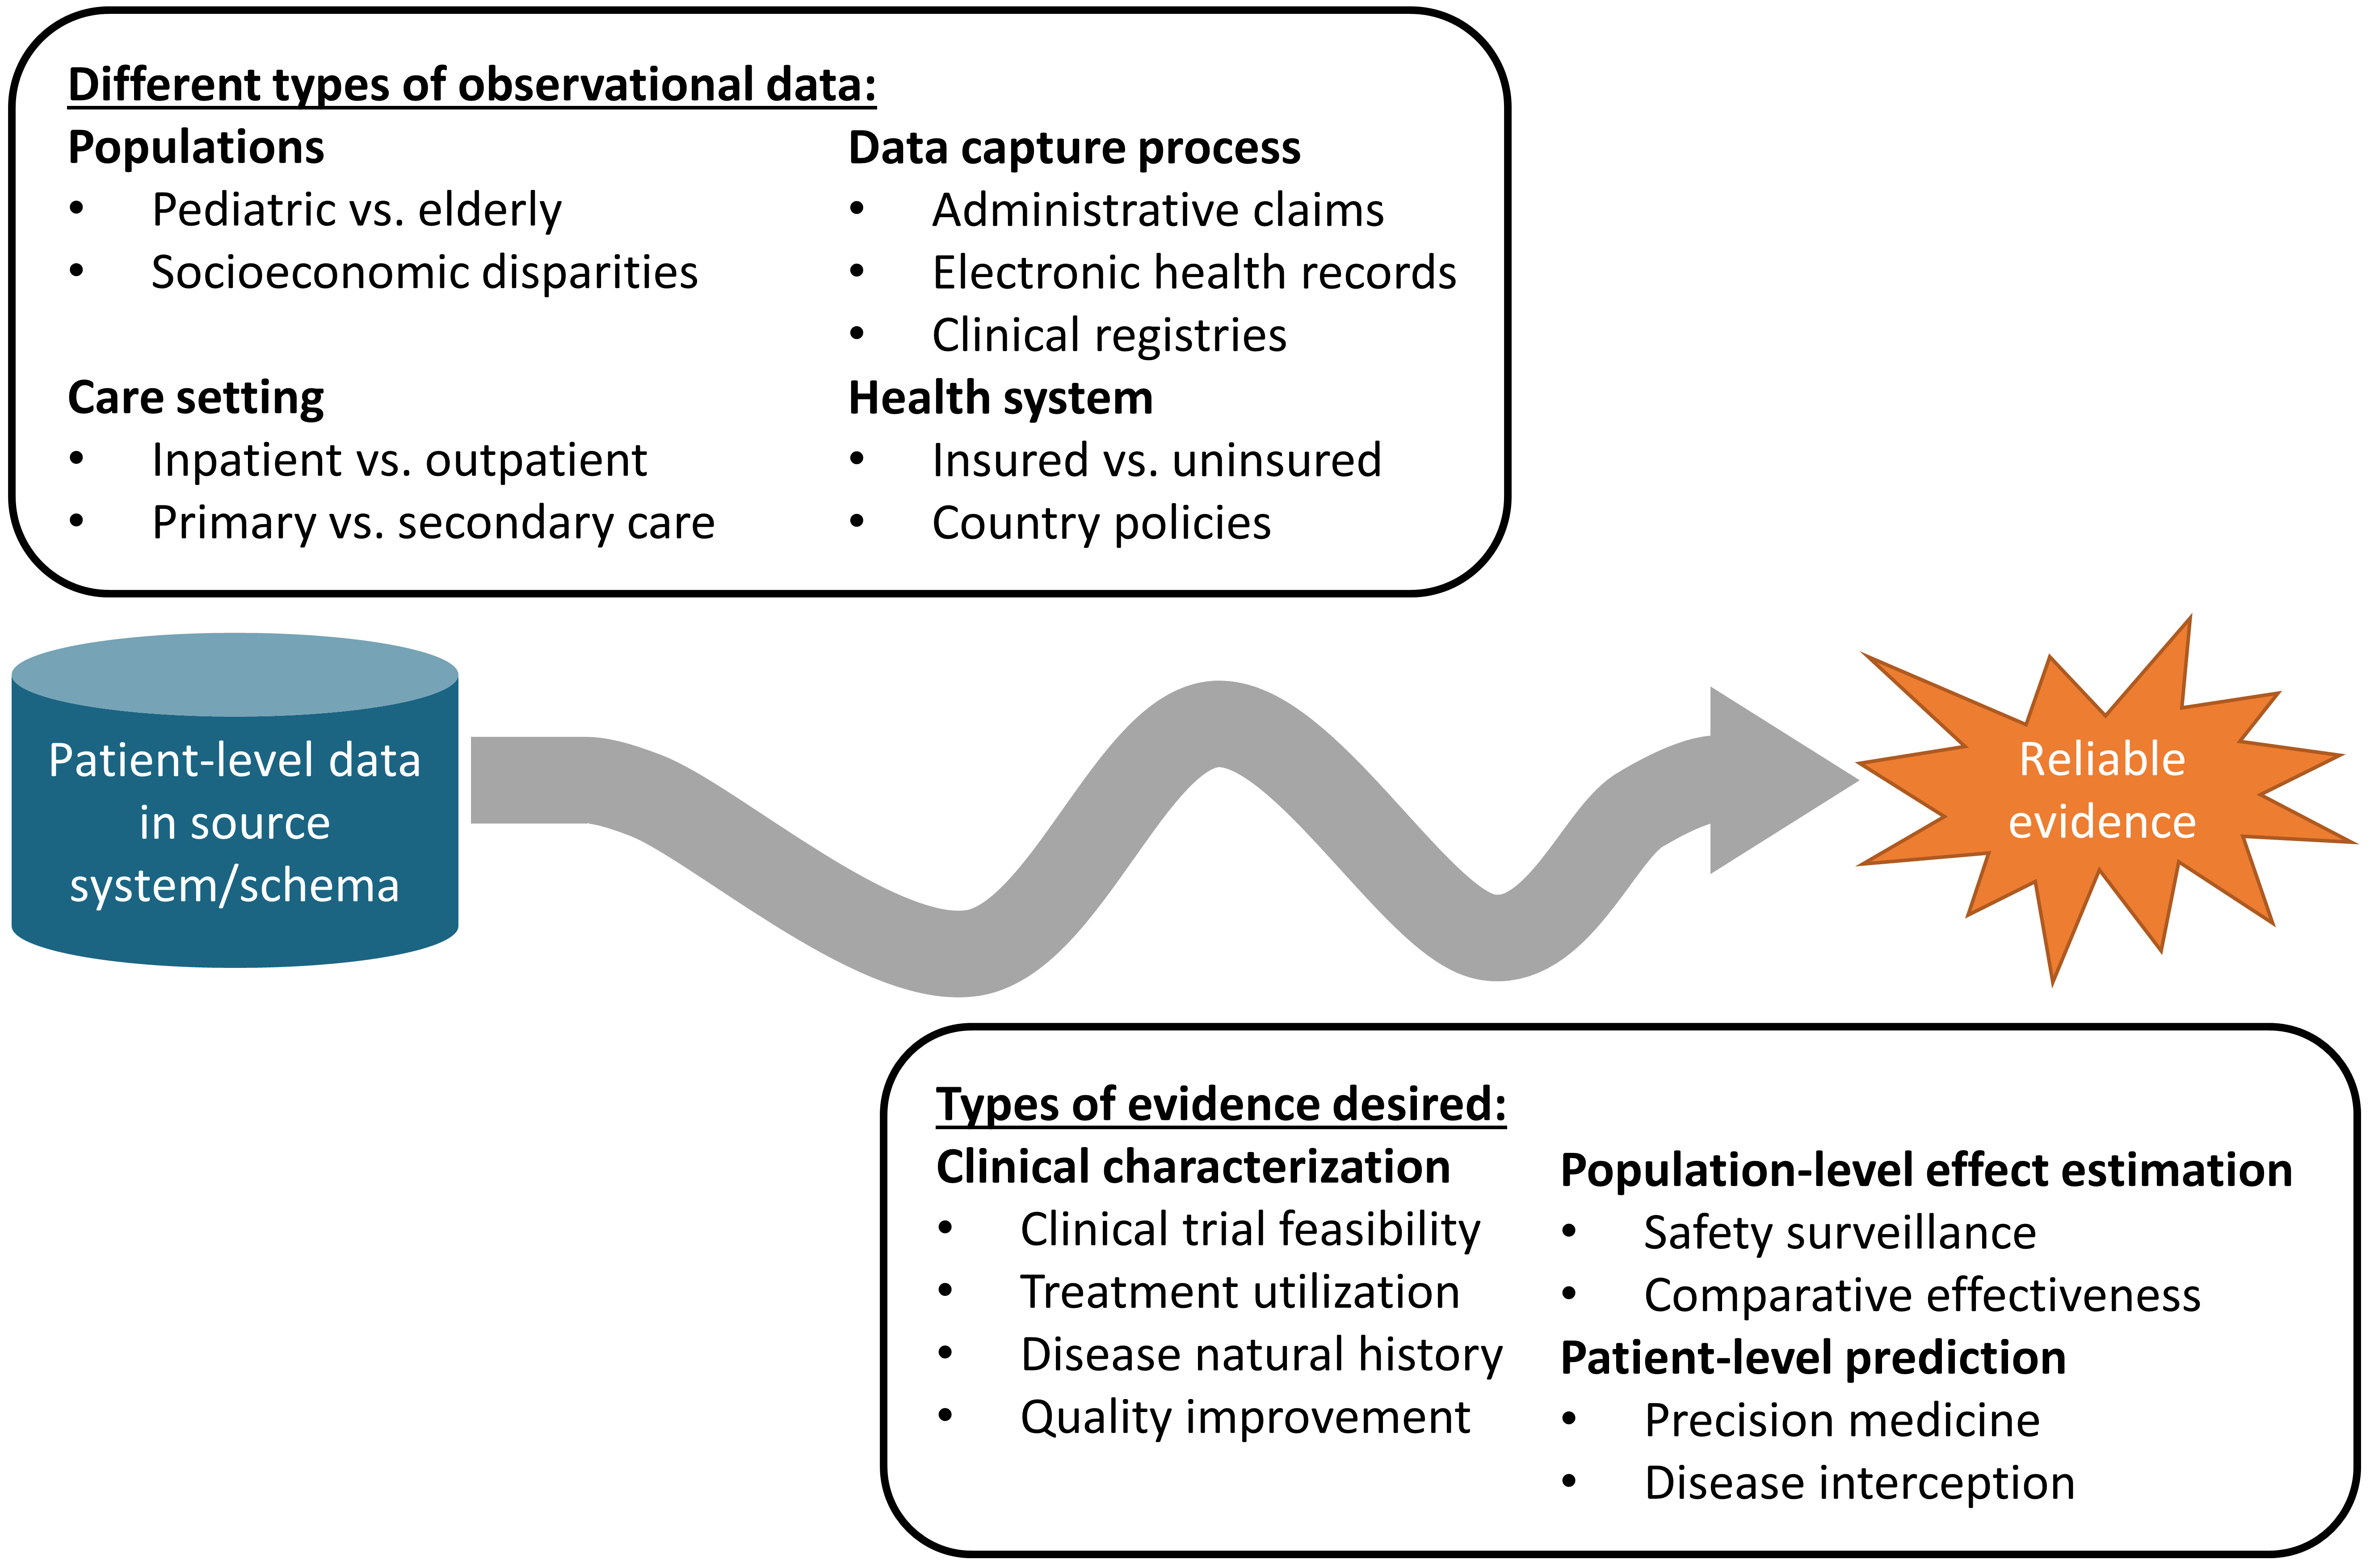
\includegraphics[width=1\linewidth]{images/OhdsiCommunity/datajourney} 

}

\caption{データからエビデンスへの旅}\label{fig:datajourney}
\end{figure}

ソースシステムには、さまざまな患者レベルのデータを収集するさまざまなタイプの観察データベースがあります。これらのデータベースは、医療システム自体と同様に多様であり、異なる人口、医療環境、データ収集プロセスを反映しています。意思決定に役立つエビデンスにもさまざまな種類があり、臨床的特性、集団レベルの推定、患者レベルの予測などの分析のユースケースによって分類することができます。 出発点(ソースデータ)と目的の目的地(エビデンス)とは別に、この課題はそのプロセスに必要とされる臨床、科学、技術的な能力の幅広さによってさらに複雑化しています。医療情報学を徹底的に理解する必要があります。これには、患者と医療従事者との診療現場でのやり取りから、管理システムや臨床システムを経て最終的な保存場所に至るまでのソースデータの完全な由来、データ収集や管理プロセスに関連する医療政策や行動インセンティブの一部として生じる可能性のある偏りの理解が含まれます。臨床上の疑問を、適切な回答を得るのに適した観察研究のデザインに変換するための疫学の原則と統計的手法を習得する必要があります。何年にもわたる縦断的追跡調査で得られた何億件もの臨床の観察結果を含む、何百万人もの患者データセットに対して、計算効率の高いデータサイエンスアルゴリズムを実装し実行する技術的能力が必要です。 また、観察データネットワークで得られた結果と他の情報源からのエビデンスを統合し、この新しい知識が医療政策や実臨床にどのような影響を与えるべきかを判断する臨床的知識も必要です。したがって、データからエビデンスを導くために必要なスキルとリソースを備えている人物は非常にまれです。むしろ、このプロセスには、すべての利害関係者が信頼し意思決定プロセスに活用できるエビデンスを生成するために、最良のデータが最適な方法で分析されるよう、複数の個人や組織が協力することが必要となる場合がほとんどです。

\section{観察医療アウトカムパートナーシップ}\label{ux89b3ux5bdfux533bux7642ux30a2ux30a6ux30c8ux30abux30e0ux30d1ux30fcux30c8ux30caux30fcux30b7ux30c3ux30d7}

観察研究におけるコラボレーションの顕著な例として、Observational Medical Outcomes Partnership(OMOP)が挙げられます。OMOPは官民パートナーシップで、米国食品医薬品局(FDA)が主導し、米国立衛生研究所(NIH)財団が運営し、製薬会社からなるコンソーシアムが資金を提供しました。製薬会社は学術研究者や医療データパートナーと協力し、観察医療データを使用した積極的な医薬品安全性監視の科学を推進する研究プログラムを確立しました。 \citep{stang2010omop} OMOPは、多様なステークホルダーによるガバナンス体制を確立し、真の医薬品安全性の関連性を特定し、偽陽性所見と区別するという課題に対して、さまざまな医療請求データやEHRデータベースに適用した場合の、代替となる疫学デザインや統計的手法のパフォーマンスを実証的に検証するための一連の方法論的実験を設計しました。

チームは集中型環境と分散型研究ネットワークの両方で、異なる観察データベースにまたがって研究を行うことの技術的な難しさを認識し、観察データの構造、内容、意味を標準化し、統計分析コードを一度作成すればすべてのデータサイトで再利用できるようにする仕組みとして、OMOP共通データモデル(CDM)を設計しました \citep{overhage2012cdm} 。OMOPの実験により、異なる医療現場から得られた異なるデータタイプを、異なるソース用語で表現し、施設間の連携と計算効率の高い分析を促進する方法で取り込むことができる共通データモデルと標準化されたボキャブラリを確立できることが実証されました。

OMOPは設立当初からオープンサイエンスのアプローチを採用し、研究デザイン、データ標準、分析コード、実証結果など、すべての成果物をパブリックドメインに置くことで透明性を高め、OMOPが実施している研究に対する信頼を構築するとともに、他者の研究目的の推進に再利用可能なコミュニティリソースを提供してきました。OMOPの当初の焦点は医薬品の安全性でしたが、OMOP CDMは、医療介入や医療制度政策の有効性の比較など、より広範な分析事例をサポートするために継続的に進化してきました。

OMOPは、大規模な実証実験の完了\citep{ryan2012omop, ryan2013omop} 、方法論の革新\citep{schuemie_2014}、安全性に関する意思決定のための観察データの適切な利用に役立つ知識の創出\citep{madigan_2013, madigan2013design}に成功しましたが、OMOPの遺産は、オープンサイエンスの原則を早期に採用し、OHDSIコミュニティの形成を促したという点で、より記憶されるかもしれません。

OMOPプロジェクトが完了し、FDAのアクティブサーベイランス活動に情報を提供するための方法論的研究という使命を果たしたとき、チームはOMOPの旅路が終わり、新たな旅路が始まったことを認識しました。OMOPの方法論的研究は、観察データから生成されるエビデンスの質を明らかに改善できる科学的ベストプラクティスに関する具体的な洞察を提供しましたが、それらのベストプラクティスの採用は遅々として進みませんでした。いくつかの障壁が特定されました。1)分析の革新よりも優先して取り組むべきであると考えられていた観察データの品質に関する根本的な懸念、2)方法論上の問題と解決策に対する概念的理解の不足、3)各自のローカル環境で独自に解決策を実行できないこと、4)これらのアプローチが各自の関心のある臨床問題に適用できるかどうかについての不確実性、などです。すべての障壁に共通する要素は、自分一人だけでは変化をもたらすために必要なすべてを持っているわけではないという感覚であり、しかし、何らかの協力的な支援があれば、すべての問題を克服できるというものでした。しかし、いくつかの分野での コラボレーションが必要でした。

\begin{itemize}
\tightlist
\item
  オープンコミュニティのデータ標準、標準化されたボキャブラリ、ETL(抽出-変換-ロード)規約の確立に向けたコラボレーション。これにより、基礎となるデータ品質に対する信頼性が高まり、構造、内容、意味論の一貫性が促進され、標準化された分析が可能になります。
\item
  医薬品の安全性にとどまらず、臨床特性、集団レベルの推定、患者レベルの予測など、より広範なベストプラクティスを確立するための方法論的研究におけるコラボレーション。方法論的研究により実証された科学的ベストプラクティスを体系化し、研究コミュニティが容易に採用できる公開ツールとして利用可能にするためのオープンソース分析開発におけるコラボレーション。
\item
  コミュニティ全体で関心のある重要な健康問題に対処する臨床応用に関するコラボレーション。データからエビデンスへの道のりを共にたどる。
\end{itemize}

このような洞察から、OHDSIは誕生しました。

\#\#オープンサイエンスの協働組織としてのOHDSI

Observational Health Data Sciences and Informatics(OHDSI、発音は「オデッセイ」)は、コミュニティが協力してより良い医療判断とケアを促進するエビデンスを生成することで、健康の改善を目指すオープンサイエンスのコミュニティです\citep{Hripcsak2015}。OHDSIは、観察医療データの適切な利用に関する科学的ベストプラクティスを確立するための方法論的研究を実施し、これらのプラクティスを一貫性があり、透明性が高く、再現可能なソリューションに体系化するオープンソースの分析ソフトウェアを開発し、臨床上の疑問に適用してエビデンスを生成し、医療政策と患者ケアの指針となることを目指しています。

\subsection{我々の使命}\label{ux6211ux3005ux306eux4f7fux547d}

\begin{quote}
健康に関する意思決定とケアを向上させるエビデンスを協力して生成することにより、コミュニティをエンパワーメントし、健康を改善する。 \index{mission}
\end{quote}

\subsection{我々のビジョン}\label{ux6211ux3005ux306eux30d3ux30b8ux30e7ux30f3}

\begin{quote}
観察研究によって健康と疾病に関する包括的な理解が得られる世界。 \index{vision}
\end{quote}

\subsection{我々の目標}\label{ux6211ux3005ux306eux76eeux6a19}

\begin{itemize}
\item
  \textbf{革新性}: 観察研究は、革新的な恩恵を得ることができる分野です。我々の仕事において、新しい方法論的アプローチを積極的に探求し、奨励します。
\item
  \textbf{再現性}: 正確で再現可能な、適切に調整されたエビデンスが健康の改善に不可欠です。
\item
  \textbf{コミュニティ}: 患者、医療従事者、研究者、そして私たちの活動に賛同する方など、誰もがOHDSIに積極的に参加いただけます。 \index{community}
\item
  \textbf{コラボレーション}: 私たちは協力して、コミュニティの参加者の現実的なニーズを優先し、対処するために協力して取り組んでいます。
\item
  \textbf{オープン性}: 私たちは私たちが生み出す方法、ツール、生成されたエビデンスなど、コミュニティの成果をすべて公開し、一般にアクセスできるよう努めています。
\item
  \textbf{有益性}: コミュニティ内の個人や組織の権利を常に保護するよう努めています。 \index{objectives}
\end{itemize}

\section{OHDSIの進展}\label{ohdsiux306eux9032ux5c55}

OHDSIは2014年の発足以来、学術界、医療製品業界、規制当局、政府、保険者、技術提供者、医療システム、臨床医、患者など、さまざまなステークホルダーから2,500人以上のコラボレーターをオンラインフォーラムに迎え入れてきました。また、コンピュータサイエンス、疫学、統計学、生物医学情報学、医療政策、臨床科学など、さまざまな分野を代表する参加者もいます。OHDSIのコラボレーターのリストは、OHDSIのウェブサイトで閲覧できます。\footnote{\url{https://www.ohdsi.org/who-we-are/collaborators/}} OHDSIの協力者マップ(図\ref{fig:collaboratormap})は、国際的なコミュニティの広さと多様性を示しています。

\begin{figure}

{\centering 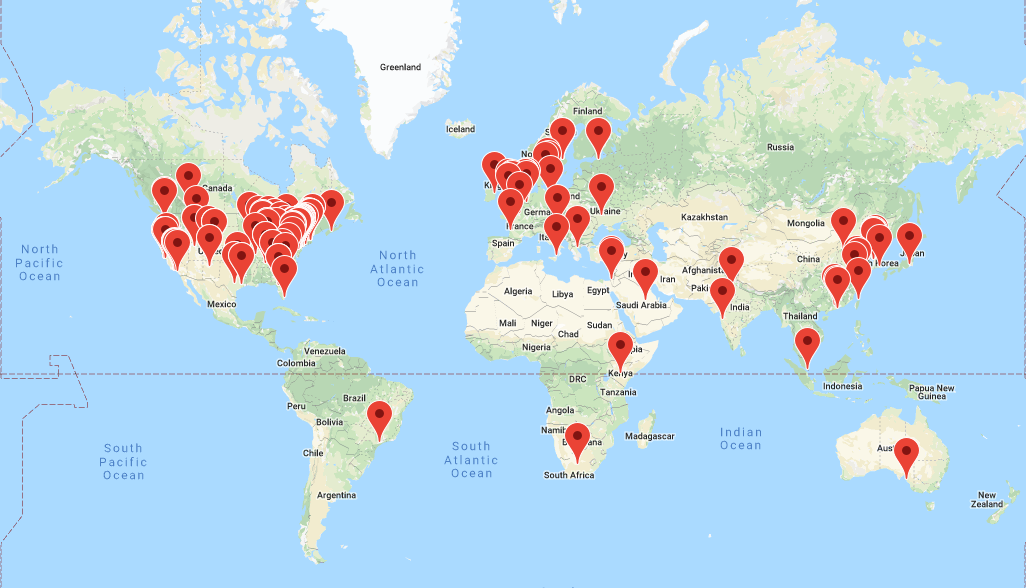
\includegraphics[width=1\linewidth]{images/OhdsiCommunity/mapOfCollaborators} 

}

\caption{2019年8月現在のOHDSI協力者の地図}\label{fig:collaboratormap}
\end{figure}

2019年8月現在、OHDSIは20か国以上から100以上の異なる医療データベースのデータネットワークを構築し、OMOP CDMというOHDSIが維持するオープンコミュニティデータ標準を用いた分散型ネットワークアプローチを適用することで10億件以上の患者記録を収集しています。分散型ネットワークとは、患者レベルのデータを組織間で共有する必要がないことを意味します。代わりに、研究に関する問いはコミュニティ内の個人によって研究プロトコルの形で提起され、エビデンスを生成する分析コードが添付されます。生成されたデータは要約統計として共有され、研究に参加するパートナー間でのみ共有されます。OHDSIの分散型ネットワークを通じて、各データパートナーは患者レベルのデータの使用について完全な自主性を維持し、それぞれの機関のデータガバナンス方針を遵守し続けます。

OHDSIの開発者コミュニティは、OMOP CDMを基盤として、以下の3つのユースケースをサポートする堅牢なオープンソース分析ツールのライブラリを作成しました。:1) 疾病の自然史、治療実態、品質向上のための臨床的特性評価;2) 医療製品の安全性監視と効果比較のための因果推論法を適用した集団レベルの効果推定;3) 精密医療や疾病予防のための機械学習アルゴリズムを適用する患者レベルの予測。OHDSIの開発者らは、OMOP CDMの採用、データの品質評価、OHDSIネットワーク研究の促進を支援するアプリケーションも開発しています。これらのツールには、RとPythonで作成されたバックエンドの統計パッケージや、HTMLとJavascriptで開発されたフロントエンドのウェブアプリケーションが含まれます。すべてのOHDSIツールはオープンソースであり、GitHubを通じて一般公開されています。\footnote{\url{https://github.com/OHDSI}}

OHDSIのオープンサイエンスコミュニティアプローチとオープンソースツールにより、観察研究は飛躍的に進歩しました。OHDSIネットワーク分析の初期の成果の一つとして、糖尿病、うつ病、高血圧という3つの慢性疾患の治療経路に関する調査が挙げられます。これはNational Academy of Scienceに掲載され、2億5000万人以上の患者のデータを対象とした11のデータソースから得られた結果を分析し、これまでに観察されたことのない治療選択に関する地理的な違いや患者の異質性を明らかにしました{[}Hripcsak7329{]} 。OHDSIは交絡因子調整のための新しい統計的手法\citep{tian_2018}や因果推論のための観察的エビデンスの妥当性評価\citep{schuemie_2018}など、複数の分野でこれらのアプローチを適用しています。てんかんの安全性監視に関する問題\citep{duke_2017}から第二選択の糖尿病治療薬の効果比較\citep{vashisht_2018}や、うつ病治療の安全性比較に関する大規模な集団レベルの効果推定研究\citep{schuemie_2018b}に至るまで、さまざまな分野で適用されています。OHDSIコミュニティは、観察医療データに機械学習アルゴリズムを適用する方法の枠組みも確立しており\citep{reps2018}、さまざまな治療領域で適用されています。\citep{johnston_2019, cepeda_2018, reps_2019}

\section{OHDSIにおける協力}\label{ohdsiux306bux304aux3051ux308bux5354ux529b}

OHDSIはエビデンスを生成するためのコラボレーションを促進することを目的としたコミュニティです。OHDSIのコラボレーターになることにはどういう意味があるのでしょうか?もしあなたがOHDSIのミッションに賛同し、データからエビデンスを生む出すまでの過程のどこかに貢献したいと思うなら、OHDSIは最適なコミュニティです。コラボレーターには、患者レベルのデータにアクセスでき、そのデータがエビデンス生成に活用されることに興味を持つ人も含まれます。コラボレーターには、科学的ベストプラクティスを確立し、代替アプローチを評価したいという方法論者も含まれます。コラボレーターには、プログラミングスキルを活かしてコミュニティ全体が利用できるツール開発に関心を持つソフトウェア開発者も含みます。コラボレーターには、重要な公衆衛生上の疑問を持ち、それに対するエビデンスを広範な医療コミュニティに提供したいと考える臨床研究者も含まれます。コラボレーターには、この共通の公衆衛生のための目的を信じ、コミュニティが自立し、そのミッションを継続できるリソースを提供したいと思う個人や組織が含まれます。また、世界中でコミュニティ活動やトレーニングセッションを主催することも含まれます。OHDSIは専門分野やステークホルダーの所属に関わらず、共通の目的に向かった個人が協力し、それぞれが貢献することで、医療の進歩に寄与できる場となることを目指しています。この取り組みに参加したい方は第 \ref{WhereToBegin} (「始める場所」)を参照し、参加方法をご確認ください。

\section{まとめ}\label{ux307eux3068ux3081}

\begin{rmdsummary}
\begin{itemize}
\item
  OHDSIのミッションは、健康に関する意思決定とケアを向上させるエビデンスを協力して生成することにより、コミュニティをエンパワーメントし、健康を改善することです。
\item
  私たちのビジョンは、観察研究が健康と疾患に関する包括的な理解をもたらす世界であり、これを革新、再現性、コミュニティ、コラボレーション、オープン性、有益性の目標を通じて達成します。
\item
  OHDSIの協力者は、オープンコミュニティのデータ標準、方法論的研究、オープンソース分析の開発、臨床応用に重点的に取り組み、データからエビデンスへの旅を改善することに取り組んでいます。
\end{itemize}
\end{rmdsummary}

\chapter{--翻訳作業中-- どこから始めようか}\label{WhereToBegin}

\emph{著者:ハメッド・アベディタシュ \& クリスティン・コストカ}

\begin{quote}
「千里の道も一歩から」 - 老子
\end{quote}

OHDSIコミュニティは、学術界、産業界、政府機関といった多くの利害関係者で構成されています。私たちの仕事は患者、医療提供者、研究者、医療システム、産業界、政府機関など、さまざまな個人や組織に利益をもたらします。この利益は、医療データ分析の質を向上させるだけでなく、これらの利害関係者にとっての医療データの有用性を向上させることによって実現されます。私たちは、観察研究が革新的な思考から大いに恩恵を受ける分野だと考えており、積極的に新しい方法論的アプローチを模索し、奨励しています。

\section{旅に参加しよう}\label{ux65c5ux306bux53c2ux52a0ux3057ux3088ux3046}

OHDSIには、患者、医療専門家、研究者、あるいは私たちの活動に賛同する人など、誰もが積極的に参加できます。OHDSIは包括的なメンバーシップモデルを維持しています。OHDSIのコラボレーターになるために会費は必要ありません。コラボレーションは手を挙げるだけの簡単なもので、毎年のOHDSI会員数に含まれます。参加は完全に任意です。コラボレーターは、毎週のコミュニティコールに参加するだけの人から、ネットワーク研究やOHDSIワーキンググループを率いる人まで、さまざまなレベルの貢献が可能です。データ保持者でなくても、活発なコミュニティメンバーとして参加できます。OHDSIコミュニティは、データ保持者、研究者、医療提供者、患者や消費者に同様にサービスを提供することを目的としています。コラボレーターのプロファイルの記録はOHDSIウェブサイトで維持され、定期的に更新されます。メンバーシップはOHDSIコミュニティコール、ワーキンググループや地域支部によって促進されます。

\subsection{OHDSIフォーラム}\label{ohdsiux30d5ux30a9ux30fcux30e9ux30e0}

OHDSIフォーラム\footnote{\url{https://forums.ohdsi.org}} は、OHDSIコミュニティのコラボレーターが投稿メッセージの形で会話ができるオンラインのディスカッションサイトです。フォーラムはツリー状のディレクトリ構造で構成されています。最上部は「カテゴリ」です。フォーラムは、関連するディスカッションのカテゴリで分けることができます。カテゴリの下にはサブフォーラムがあり、これらのサブフォーラムにはさらにサブフォーラムがあります。トピック(一般にはスレッドと呼ばれる)はサブフォーラムの最下層にあり、ここでフォーラムメンバーはディスカッションや投稿を始められます。

OHDSIフォーラムには、次のようなコンテンツのカテゴリがあります:

\begin{itemize}
\tightlist
\item
  \textbf{一般:} OHDSIコミュニティに関する一般的なディスカッションと参加方法
\item
  \textbf{実装者:} 共通データモデルとOHDSI分析フレームワークをローカル環境に実装する方法についてのディスカッション
\item
  \textbf{開発者:} OHDSIアプリケーションや他のOMOP CDMを活用するツールのオープンソース開発についてのディスカッション
\item
  \textbf{研究者:} CDMベースの研究に関するディスカッション(エビデンス生成、共同研究、統計手法やOHDSI研究ネットワークに関連するその他のトピックを含む)
\item
  \textbf{CDMビルダー:} 要件、ボキャブラリ、技術的側面を含む進行中のCDM開発に関するディスカッション
\item
  \textbf{語彙ユーザー:} ボキャブラリコンテンツに関するディスカッション
\item
  \textbf{地域支部(例:韓国、中国、ヨーロッパ):} OMOP実装やOHDSIコミュニティ活動に関連する、母国語での地域のディスカッション
\end{itemize}

自分のトピックを投稿するには、アカウントにサインアップする必要があります。フォーラムのアカウントを取得し、一般的なトピックの「Welcome to OHDSI! - Please introduce yourself(OHDSIへようこそ!-自己紹介をお願いします」というスレッドで自己紹介することをお勧めします。返信では1) 自己紹介と自分の仕事について簡単に教えてください、2) コミュニティでどのように貢献したいか教えてください(例:ソフトウェア開発、研究実施、研究論文の執筆など)。これでOHDSIの旅が始まります!ここから、ディスカッションに参加することをお勧めします。質問したり、新しいアイデアを議論したり、コラボレーションしたりするための手段として、OHDSIコミュニティはフォーラムを使用することを推奨しています。 \index{forum}

\begin{rmdimportant}
トピックを選択して「ウォッチ」することができます。つまり、ウォッチしているトピックに新しい投稿が追加されるたびにメールが届き、その投稿にメールで直接返信できるようになります。一般的なスレッドをウォッチして、今後の会議の議題や、コラボレーションの機会に関する詳細を受け取ったり、毎週のOHDSIダイジェストを直接受信トレイに配信しましょう!
\end{rmdimportant}

\subsection{OHDSIイベント}\label{ohdsiux30a4ux30d9ux30f3ux30c8}

OHDSIは、コラボレーター同士が学び合い、将来の協力を促進する機会を提供するため、定期的に対面イベントを開催しています。これらのイベントはOHDSIウェブサイトで通知され、参加を希望する人は誰でも無料で参加できます。

OHDSIシンポジウムは、米国、ヨーロッパ、アジアで毎年開催される学術会議で、コラボレーターが全体会議、ポスター発表、ソフトウェアのデモを通じて最新の研究を発表できます。OHDSIシンポジウムはネットワーキングのための素晴らしい場であり、コミュニティ全体での最新の進歩について学ぶ機会です。OHDSIシンポジウムは通常、OHDSIチュートリアルが併設されており、コースの講師である OHDSI 共同研究者が教えるもので、コミュニティの新規参加者に、データ標準や分析のベストプラクティスに関するトピックについて実践的な取り組みを行う機会を提供します。これらのチュートリアルは通常ビデオ録画され、イベント後にOHDSIウェブサイトで公開され、イベントに参加できなかった人も利用できます。

OHDSIコラボレーターの対面イベントは、通常は共通の関心事の問題に焦点を当てた小規模なフォーラムです。過去のイベントには、フェノタイプ・ハッカソン、データ品質ハッカソン、オープンソースソフトウェアのドキュメンテーション・ハッカソンなどがあります。OHDSIは、複数のStudy-a-thonイベントを主催してきました。この複数日にわたるセッションの目的は、適切な観察分析を設計・実装し、OHDSIネットワーク全体で研究を実行し、一般への普及のためにエビデンスを統合することにより、特定の研究問題に関してチームとして協力することです。これらのすべてのイベントにおいて、共通の問題を解決したいという共通の願いがあるだけでなく、共同で問題解決を行うプロセスを学び、継続的な改善を促す歓迎的な環境を提供することにも共通の関心があります。

OHDSIコミュニティのパワーをもっと学びましょう。過去のシンポジウム、対面会議を検索し、OHDSIチュートリアルを視聴ください。OHDSIウェブサイトの\href{https://www.ohdsi.org/past-events/}{過去のイベント}セクションから視聴できます。過去のイベントは定期的に更新され、コミュニティイベントはアーカイブされています。

\subsection{OHDSIコミュニティコール}\label{ohdsiux30b3ux30dfux30e5ux30cbux30c6ux30a3ux30b3ux30fcux30eb}

OHDSI コミュニティ コールは、OHDSI コミュニティ内で進行中の活動にスポットライトを当てる機会です。毎週火曜日の午前11時から12時(東部標準時)に開催される電話会議は、OHDSIコミュニティが集まり、最近の開発を共有し、個々のコラボレーター、ワーキンググループ、コミュニティ全体の成果を認識する時間です。毎週の会議は記録され、プレゼンテーションはOHDSIウェブサイトのリソースにアーカイブされます。

OHDSIコラボレーターは、毎週のこの電話会議への参加を歓迎され、コミュニティディスカッションのトピックを提案することが奨励されています。OHDSIコミュニティコールは、研究成果を共有し、進行中の作業に対するフィードバックを求め、開発中のオープンソースソフトウェアツールをデモンストレーションし、データモデリングと分析のためのコミュニティベストプラクティスを議論し、助成金/出版物/会議ワークショップのための将来のコラボレーションの機会をブレインストーミングするフォーラムとなります。OHDSIコラボレーター会議のトピックを持っているコラボレーターは、OHDSIフォーラムに意見を投稿ください。

OHDSI コミュニティの新規参加者として、OHDSIネットワーク全体で何が起こっているかを把握するために、このコールシリーズをカレンダーに追加することをお勧めします。OHDSIコールに参加する場合は、OHDSIフォーラムでアナウンスを確認してください。\href{https://forums.ohdsi.org/}{OHDSIフォーラム}コミュニティコールのトピックは週ごとに異なります。OHDSIフォーラムのOHDSIウィークリーダイジェストで、毎週のプレゼンテーションのトピックの詳細情報を確認することもできます。新規参加者は、初回のコールで自己紹介し、自分自身、経歴、OHDSIに参加した理由についてコミュニティに話すよう求められます。\index{コミュニティ!コミュニティコール}

\subsection{OHDSIワークグループ}\label{ohdsiux30efux30fcux30afux30b0ux30ebux30fcux30d7}

OHDSI には、ワークグループチームが主導するさまざまな進行中のプロジェクトがあります。各ワークグループにはそれぞれリーダーシップ チームがあり、プロジェクトの目的、目標、コミュニティに提供される成果物を決定します。ワークグループには、プロジェクトの目的と目標に貢献することに関心のあるすべての人が参加できます。ワークグループは、長期にわたる戦略的な目的の場合もあれば、コミュニティの特定のニーズを満たすための短期プロジェクトである場合もあります。ワークグループの会議の頻度は、プロジェクトリーダーシップによって決定され、グループごとに異なります。アクティブなワークグループのリストは、OHDSI Wiki OHDSIWiki{]}(\href{https://www.ohdsi.org/web/wiki/doku.php?id=projects:overview}{https://www.ohdsi.org/web/wiki/doku.php?id=projects:overview)}で管理されています)\{.uri\}。 \index{作業グループ}

表 \ref{tab:OHDSIworkgroups} は、アクティブなOHDSI作業グループのクイックリファレンスです。是非コールに参加して、より多くを学ぶことをお勧めします。

表 \label{tab:OHDSIworkgroups} 注目すべきOHDSI作業グループ

\begin{longtable}[]{@{}
  >{\raggedright\arraybackslash}p{(\columnwidth - 4\tabcolsep) * \real{0.3333}}
  >{\raggedright\arraybackslash}p{(\columnwidth - 4\tabcolsep) * \real{0.3333}}
  >{\raggedright\arraybackslash}p{(\columnwidth - 4\tabcolsep) * \real{0.3333}}@{}}
\toprule\noalign{}
\begin{minipage}[b]{\linewidth}\raggedright
ワークグループ名
\end{minipage} & \begin{minipage}[b]{\linewidth}\raggedright
目的
\end{minipage} & \begin{minipage}[b]{\linewidth}\raggedright
対象参加者
\end{minipage} \\
\midrule\noalign{}
\endhead
\bottomrule\noalign{}
\endlastfoot
Atlas \& WebAPI & AtlasとWebAPIは、OMOP共通データモデルを基盤として構築し、標準化された分析機能を提供するOHDSIオープンソースソフトウェアアーキテクチャの一部です。 & オープンソースのAtlas/WebAPIプラットフォームを改善し、貢献することを目指すJava \& JavaScriptソフトウェア開発者 \\
CDM \& Vocabulary & 臨床患者データに適用される体系的で、標準化された大規模な分析を目的として、OMOP共通データモデルの開発を継続します。他のワーキング グループによって開発された標準化された分析をサポートするため、国際的なコーディングシステムと患者ケアの臨床的側面のカバレッジを拡大することで、標準化されたボキャブラリの品質を向上させます。 & OMOP共通データモデルと標準化ボキャブラリの改善に関心があり、すべてのニーズとユースケースに対応できる人 \\
Genomics & OMOP CDMを拡張して、患者のゲノムデータを組み込みます。グループは、さまざまなシーケンスプロセスからの遺伝子変異に関する情報を保存できる CDM 互換スキーマを定義します。 & すべての人が参加可能 \\
Population-Level Estimation & 正確で信頼性が高く、再現性のある集団レベルの効果推定につながる観察研究のための科学的手法を開発し、コミュニティによるこれらの手法の使用を促進します。 & すべての人が参加可能 \\
Natural Language Processing & OHDSI傘下の観察研究で、電子健康記録(EHR)のテキスト情報の使用を促進します。この目的を促進するため、グループはOHDSIコミュニティによる研究に臨床テキストを利用するために実装できる方法とソフトウェアを開発します。 & すべての人が参加可能 \\
患者レベルの予測 & 複数の対象とするアウトカムに用いることができ、対象とするあらゆる患者サブグループからの観察医療データに適用します。正確で十分に調整された患者中心の予測モデルを開発するため、標準化されたプロセスを確立します。 & すべての人が参加可能 \\
Gold Standard Phenotype Library & OHDSIコミュニティのメンバーが、コミュニティで検証されたコホート定義を研究やその他の活動のために見つけ、評価し、利用できるようにします。 & フェノタイプのキュレーションと検証に関心のあるすべての人が参加可能 \\
FHIR Workgroup & OHDSI FHIR統合のロードマップを確立し、OHDSIベースの観察研究のためにEHRコミュニティのFHIR実装とデータを活用し、FHIRベースのツールとAPIを通じてOHDSIデータと研究結果を普及するための推奨事項を、より広範なコミュニティに提供します。 & 相互運用性に関心のあるすべての人が参加可能 \\
GIS & OMOP CDMを拡張し、患者の環境曝露の履歴をその臨床フェノタイプと関連付けるためにOHDSIツールを活用します。 & 健康関連の地理属性に興味のあるすべての人が参加可能 \\
Clinical Trials & OHDSIプラットフォームとエコシステムがあらゆる面で試験を支援できる臨床試験のユースケースを理解し、サポートする OHDSI ツールの更新の推進を支援します。 & 臨床試験に興味のあるすべての人が参加可能 \\
THEMIS & THEMIS の目的は、OMOP CDM 規則を超える標準規則を開発し、各 OMOP サイトで設計された ETL プロトコルが最高品質で、再現可能かつ効率的であることを保証することです。 & ETL標準化に関心のあるすべての人が参加可能 \\
Metadata \& Annotations & 私たちの目標は、人間と機械が作成したメタデータと注釈を 共通データモデル に保存するための標準プロセスを定義し、研究者が観察データセットに関する有用なデータ成果物を利用して作成できるようにすることです。 & すべての人が参加可能 \\
Patient Generated Health Data (PGHD) & & \\
この ワーキンググループの目標は、スマートフォン/アプリ/ウェアラブル デバイスから生成される PGHD の ETL 規則、臨床データとの統合プロセス、分析プロセスを開発することです。 & すべての人が参加可能 & \\
Women of OHDSI & OHDSI & コミュニティ内の女性が集まり、科学、技術、工学、数学 (STEM) 分野で働く女性として直面する課題を話し合うためのフォーラムを提供します。女性が意見を共有し、懸念を表明し、OHDSI コミュニティが STEM 分野の女性をどのようにサポートできるかについてアイデアを提案します。最終的には女性がコミュニティ内やそれぞれの分野でリーダーになれるよう、刺激となるような議論を促進することを目指しています。 \\
Steering Committee & OHDSIのすべての活動とイベントが、成長を続けるコミュニティのニーズに合致していることを確認することで、OHDSI の使命、ビジョン、価値観を維持します。さらに、このグループは、OHDSI の将来の方向性についてガイダンスを提供することで、コロンビアに拠点を置く OHDSI 調整センターの諮問グループとして機能します。 & コミュニティ内のリーダー \\
\end{longtable}

\subsection{OHDSI地域支部}\label{ohdsiux5730ux57dfux652fux90e8}

OHDSI 地域支部は、地理的な地域に所在し、地域特有の問題に対処するため、ローカル ネットワークイベントや会議を開催したいと考えている OHDSI コラボレーターのグループです。現在、OHDSI地域支部は、ヨーロッパ\footnote{\url{https://www.ohdsi-europe.org/}}、韓国\footnote{\url{https://forums.ohdsi.org/c/For-collaborators-wishing-to-communicate-in-Korean}}、中国\footnote{\url{https://ohdsichina.org/}}にあります。ご自身の地域で OHDSI 地域支部を設立したい場合は、OHDSI Webサイトで説明されているOHDSI地域支部のプロセスに従って設立できます。

\subsection{OHDSIリサーチネットワーク}\label{ohdsiux30eaux30b5ux30fcux30c1ux30cdux30c3ux30c8ux30efux30fcux30af}

OHDSI のコラボレーターの多くは、データをOMOP共通データモデルに変換することに関心を持っています。OHDSI研究ネットワークは、抽出、変換、ロード(ETL)プロセスを経てOMOPに準拠した観測データベースの多様なグローバルコミュニティを表しています。OHDSIコミュニティでの取り組みにデータの変換が含まれる場合は、OMOP CDMとボキャブラリに関するチュートリアル、変換を支援する無料で利用可能なツール、特定のドメインやデータ変換の種類を対象とするワークグループなど、取り組みを支援する多数のコミュニティリソースがあります。OHDSIのコラボレーターは、OHDSIフォーラムを利用して、CDM変換中に発生する課題について話し合い、トラブルシューティングすることを推奨されます。

\section{どこにフィットするか}\label{ux3069ux3053ux306bux30d5ux30a3ux30c3ux30c8ux3059ux308bux304b}

ここまで読んで、あなたは「私は OHDSI コミュニティのどこに属しているのだろう?」と疑問に思っているかもしれません。

\textbf{私は臨床研究者で、研究を始めたいと思っています。} 特定の質問に答えるためにOHDSIリサーチネットワークを使用したい臨床研究者であるなら、たとえば論文を発表したいと考えているなら、あなたは正しい場所にいます。OHDSIフォーラムの\href{https://forums.ohdsi.org/c/researchers}{OHDSIリサーチャーズトピック}にアイデアを投稿することから始めましょう。これにより、同様の関心を持つ研究者とつながることができます。OHDSIは論文の出版を好んでおり、リサーチクエスチョンを分析や迅速に分析や論文にしていくための多くのリソースを提供しています。詳細は第\ref{Characterization}、\ref{PopulationLevelEstimation}、\ref{PatientLevelPrediction}章をご覧ください。

\textbf{私はOHDSIコミュニティが発信する情報を読んで利用したいと思っています。} 患者、臨床医、医療の専門家のいずれであっても、OHDSI は健康アウトカムをよりよく理解するのに役立つ高品質のエビデンスを提供したいと考えています。コードを書くのは久しぶりかもしれません。プログラムを書いたことがないかもしれません。あなたにはこのコミュニティに居場所があります。私たちはあなたを\emph{エビデンスの消費者}と呼びます。あなたはOHDSIの研究を行動に移す人です。あなたは OHDSI がどのようなエビデンスを生成したか、または生成中であるかを知るためにふるいにかけており、おそらく自分に関連する質問を提案したいとも思っているでしょう。私たちはあなたがディスカッションに参加することを歓迎します。\href{http://forums.ohdsi.org}{OHDSIフォーラム}で質問を始めましょう。コミュニティコールに参加し、最新の研究について聞いてください。OHDSIシンポジウムや対面ミーティングに参加してコミュニティと直接交流しましょう。あなたの質問はOHDSIコミュニティの重要な部分です。声を上げて、あなたが探しているエビデンスについて、私たちがさらに知る手助けをしてください!

\textbf{私は医療のリーダーとして働いています。データ所有者、またはその代表者であるかもしれません。組織にとってのOMOP CDMとOHDSI分析ツールの有用性を評価しています。} 組織の管理者/リーダーとして、あなたはOHDSIについて聞いたことがあり、OMOP CDMがあなたのユースケースにどのように役立つかを知りたいと思っているかもしれません。\href{https://www.ohdsi.org/past-events/}{OHDSI過去のイベント}資料に目を通し、研究内容を確認ください。コミュニティコールに参加して、ただ聞くだけでも構いません。Chapter \ref{DataAnalyticsUseCases}第7章(データ分析のユースケース)を読むと、OMOP CDMやOHDSI分析ツールで実現できる研究の種類を理解するのに役立つかもしれません。OHDSIコミュニティは、あなたの旅をサポートします。興味のある具体的な分野がある場合は遠慮せずに発言し、事例を尋ねてください。世界中の200以上の組織がOHDSIで協力しており、コミュニティの価値を示すための多くの成功事例があります。

\textbf{私はデータベース管理者で、私の機関のデータをETLまたはOMOP CDMに変換したいと考えています。} データを「OMOP」することは、斬新で価値のある取り組みです。ETLプロセスを始めたばかりの場合、\href{https://www.ohdsi-europe.org/images/symposium-2019/tutorials/OHDSI_Vocabulary_CDM_Tutorial.pdf}{OHDSIコミュニティのETLチュートリアルスライド}を参照するか、今後開催されるOHDSIシンポジウムに登録したりしてください。THEMIS作業グループのコールに参加し、OHDSIフォーラムで質問することも考えてみてください。OMOP CDMの実装を成功に導く支援となる知識がコミュニティには豊富にあります。遠慮しないでください!

\textbf{私はバイオ統計学者かつ、またはメソッドの開発者で、OHDSIツールスタックへの貢献に興味があります。}Rに精通しており、Gitにコミットする方法を知っています。何よりも、OHDSIメソッドライブラリに専門知識を持ち込み、これらの方法論をさらに発展させたいと思っています。まずは、集団レベルの推定または患者レベルの予測のワークグループコールに参加し、現在のコミュニティの優先事項について詳しく聞くことをお勧めします。OHDSIツールを使用する際、該当するGitHubリポジトリ(例:SQL Renderパッケージの問題であれば、OHDSI/SqlRenderのGitHubリポジトリに提出します)に問題を報告することもできます。皆さんの貢献をお待ちしています!

\textbf{私はソフトウェア開発者で、OHDSIツールスタックを補完するツールの構築に関心があります。} コミュニティへようこそ!OHDSIのミッションの一環として、私たちのツールはApacheライセンスの下でオープンソースとして管理されています。OHDSIツールスタックを補完するソリューションの開発を歓迎しています。ワーキンググループに参加し、アイデアを提案ください。OHDSIはオープンサイエンスとオープンコラボレーションに多大な投資をしていることに留意ください。独自のアルゴリズムとソフトウェアソリューションは歓迎しますが、私たちのソフトウェア開発の主な焦点ではありません。

\textbf{私はコンサルタントで、OHDSIコミュニティに助言したいと考えています。} コミュニティへようこそ!あなたの専門知識は貴重であり、高く評価されています。必要に応じて、OHDSIフォーラムでサービスを宣伝することができます。OHDSIチュートリアルに参加ください。また、年間を通じてシンポジウムの議事録や OHDSI の対面ミーティングで専門知識を提供して貢献することを検討ください。

\textbf{私は学生で、OHDSIについてもっと学びたいと思っています。} あなたは正しい場所にいます!OHDSIコミュニティコールに参加し、自己紹介することを考えてみてください。OHDSIチュートリアルを詳しく調べたり、OHDSIシンポジウムや対面ミーティングに参加してOHDSIコミュニティが提供する方法とツールについてさらに学ぶことをお勧めします。特定の研究に関心がある場合は、OHDSIフォーラムの研究者トピックに投稿してお知らせください。多くの組織がOHDSIが後援する研究の機会(例:ポスドク、研究フェローシップ)を提供しています。OHDSIフォーラムでは、これらの機会などに関する最新情報を提供しています。

\section{まとめ}\label{ux307eux3068ux3081-1}

\begin{rmdsummary}
\begin{itemize}
\tightlist
\item
  OHDSIコミュニティに参加するのは、挨拶するのと同じくらい簡単です。\textbf{OHDSIフォーラム}に投稿し、コミュニティコールに参加ください。
\item
  研究やETLに関する質問をOHDSIフォーラムに投稿ください。
\end{itemize}
\end{rmdsummary}

\chapter{--翻訳作業中-- オープンサイエンス}\label{OpenScience}

\index{オープンサイエンス}

\emph{章リーダー: キース・バン・ボコーブ}

OHDSIコミュニティの発足当初から、オープンソースソフトウェア利用、すべての会議の議事録や資料の公開、生成された医療的エビデンスの透明性あるオープンアクセスによる公開など、オープンサイエンスの価値観に基づいて国際的な共同研究体制を確立することが目標とされてきました。しかし、オープンサイエンスとは具体的にはどのようなものでしょうか? また、プライバシーへの配慮が非常に重要であり、通常は正当な理由から公開されていない医療データに関してOHDSIはどのようにオープンサイエンスやオープンデータ戦略を構築できるのでしょうか。? 分析の再現性がなぜそれほど重要なのでしょうか。OHDSIコミュニティはこれをどのようにしてこれを実現しようとしているのでしょうか。 本章ではこれらの疑問について触れていきます。

\section{オープンサイエンス}\label{ux30aaux30fcux30d7ux30f3ux30b5ux30a4ux30a8ux30f3ux30b9}

「オープンサイエンス」という用語は1990年代から使われていましたが実際に注目を集めるようになったのは2010年代で、OHDSIが誕生したのと同じ時期です。Wikipedia \citep{wiki:Open_science} ではこれを「科学的研究(出版物、データ、物理的サンプル、ソフトウェアを含む)とその普及を、アマチュアか専門家を問わず、探求心のあるあらゆるレベルの人々が利用できるようにする運動」と定義しており、通常は共同ネットワークを通じて開発されると述べています。OHDSIコミュニティは明確には「オープンサイエンス」集団またはネットワークとして位置づけられたことはありませんが、この用語はOHDSIの基本的な概念や原則を説明する際にこの用語が頻繁に使われています。例えば、2015年にはジョン・デュークがOHDSIを「医療エビデンス生成へのオープンサイエンスアプローチ」と表現し、2019年にはEHDENコンソーシアムの紹介ウェビナーでOHDSIネットワークアプローチを「21世紀のリアルワールドオープンサイエンス」として称賛しました。実際、この章で詳しく見ていくように、オープンサイエンスの実践の多くは今日のOHDSIコミュニティに見出すことができます。OHDSIコミュニティは、医療におけるエビデンス生成の透明性と信頼性を向上させるという共通の願いから生まれた草の根的なオープンサイエンスの集合体である、という見方もできるでしょう。

オープンサイエンスまたは「サイエンス2.0」のアプローチ\citep{wiki:Science_2.0}は、現在の科学的手法における多くの認識された問題に対処することを意味します。情報技術はデータの生成と分析方法の爆発的な増加をもたらし、個々の研究者にとっては、専門分野で発表されるすべての文献を把握するのは非常に困難になっています。これは、本業として診療をしながらも最新の医学的エビデンスに遅れずについていく必要のある医師にとっては、なおさらのことです。さらに、多くの試験が統計設計の不備、出版バイアス、p-hacking、その他の同様の統計的問題に直面し、再現は困難であるという懸念が高まっています。こうした懸念を修正する従来の方法である論文の査読では、こうした問題を特定し、対処できないことがよくあります。2018年の『Nature』誌の特集号「再現不可能な研究における課題」に関する2018年のNature特集版{[}\^{}3{]}には、この問題の例がいくつか紹介されています。ある分野の論文に系統的な査読を適用しようとした著者グループは、さまざまな理由により、彼らが指摘したエラーを修正してもらうのが非常に難しいことを発見しました。特に、最初から欠陥のあるデザインの試験は修正が難しかったのです。ロナルド・フィッシャーの言葉によると、「試験が終了してから統計学者に相談することは、単に死後解剖を依頼するようなものだ。おそらく、その試験がなぜ失敗したのかを教えてくれるだろう」\citep{wikiquote:Ronald_Fisher} 著者らは、ランダム化デザインの不備による統計的有意性についての誤った結論、メタ分析における誤算、不適切なベースライン比較など、一般的な統計上の問題に直面しました。\citep{allison_2016} 同じ論文集の別の論文では、物理学の経験を例に挙げ、完全な再現性を実現するには、基礎データへのアクセスを提供するだけでなく、データ処理と分析のスクリプトを公開し、適切に文書化することが重要であると主張しています。\citep{Chen2018}

OHDSIコミュニティはこれらの課題に対して独自の方法で取り組んでおり、大規模な医療エビデンスの生成の重要性を強調しています。\citet{schuemie_2018bによると}、現在のパラダイムは「信頼性が不明な独自の研究デザインを用いて、1つずつ推定値を生成し、1つずつ推定値を公表(または不公表)することに重点を置いている」一方で、OHDSIコミュニティは「一貫性のある標準化された方法を用いた高スループットの観察研究を提唱し、評価、較正、偏りのない普及を可能にすることで、より信頼性が高く完全なエビデンスベースを生成する」としています。これは、OMOP 共通データモデルにデータをマッピングする医療データソースのネットワーク、誰もが利用・検証可能なオープンソース分析コード、howoften.org で公開されている疾患発生状況などの大規模なベースラインデータの組み合わせによって実現されます。以下では、具体的な例を挙げ、オープンスタンダード、オープンソース、オープンデータ、オープンディスカッションの4つの原則を指針として、OHDSIのオープンサイエンスのアプローチについてさらに詳しく説明します。本章の締めくくりとして、オープンサイエンスの観点からOHDSIのFAIR原則と展望について簡単に言及します。

\section{オープンサイエンスの実践: the Study-a-Thon}\label{ux30aaux30fcux30d7ux30f3ux30b5ux30a4ux30a8ux30f3ux30b9ux306eux5b9fux8df5-the-study-a-thon}

\index{study-a-thon}

コミュニティにおける最近の動きとして、「study-a-thon」の出現が挙げられます。これは、OMOPデータモデルとOHDSIツールを使用して、臨床的に重要な研究課題の答えを導くことを目的とした、多分野にわたる科学者グループの短期集中型の対面式集会です。その好例が、2018年のオックスフォード研究マラソンです。この研究マラソンについては、EHDENのウェビナーで説明されており、そのプロセスが詳しく紹介されているほか、公開されている結果も強調されています。研究マラソンに先立ち、参加者は医学的に関連性の高い研究課題を提案し、研究マラソンで研究する1つもしくは複数の研究課題が選定されます。OMOP形式の患者レベルデータにアクセスでき、これらのデータソースでクエリを実行できる参加者にデータが提供されます。実際のstudy-a-thonの時間の多くは、統計的アプローチ(\ref{WhereToBegin}章参照)、データソースの適合性、インタラクティブに作成される結果、およびこれらの結果から必然的に生じる追加の質問について議論することに費やされます。オックスフォード大学でのstudy-a-thonの場合は、さまざまな人工膝関節置換術の術後の有害作用の研究に焦点が当てられ、study-a-thonの期間中にOHDSIフォーラムとツールを使用してインタラクティブに結果が発表されました(Chapter \ref{OhdsiAnalyticsTools}参照)。ATLASなどのOHDSIツールは、コホート定義の迅速な作成、交換、議論、テストを可能にし、問題定義と方法の選択に関するコンセンサスを達成する初期プロセスを大幅にスピードアップさせます。関連するデータソースがOMOP共通データモデルを使用し、OHDSIのオープンソース患者レベル予測パッケージが利用可能になった\ref{PatientLevelPrediction}おかげで、90日間の術後死亡率の予測モデルを1日で作成し、翌日には複数の大規模データソースでそのモデルを外部検証することが可能になりました。また、このマラソン研究は、従来の学術論文(「人工膝関節全置換術後の有害事象に対する患者レベル予測モデルの開発と検証」)の執筆にもつながりました。この論文は、査読に数ヶ月を要しました。しかし、数億件の患者記録を網羅する複数の医療データベースの分析スクリプトと結果が、わずか1週間でゼロから構想、作成、公開されたという事実は、OHDSIが医学にもたらす根本的な改善を示しています。これにより、エビデンスが利用可能になるまでの期間が数ヶ月から数日に短縮されます。

\section{オープンスタンダード}\label{ux30aaux30fcux30d7ux30f3ux30b9ux30bfux30f3ux30c0ux30fcux30c9}

\index{オープンサイエンス!open standards}

OHDSIコミュニティで維持されている非常に重要なコミュニティリソースは、OMOP共通データモデル(第 \ref{CommonDataModel}章参照)と関連する標準化ボキャブラリ(第 \ref{StandardizedVocabularies}章参照)です。このモデル自体は観察医療データを収集することを目的としており、もともとは薬物、処置、デバイスなどの曝露と、状態や測定値などの結果との関連性を分析することを目的としていました。様々な分析用とに合わせて拡張されてきました(詳しくは第\ref{DataAnalyticsUseCases}章参照)。しかし、世界中のさまざまなコーディングシステム、医療パラダイム、さまざまなタイプの医療ソースからヘルスケアデータを調和させるには、ソースコードとその最も近い標準化された対応コードとの間の膨大な「マッピング」が必要になります。OMOP標準化ボキャブラリは第 \ref{DataAnalyticsUseCases}章でさらに詳しく説明されており、世界中で使用されている数百の医療コーディングシステムからのマッピングを含み、OHDSIのAthenaツールを通じて閲覧可能です。これらのボキャブラリとマッピングを無料で利用可能なコミュニティリソースとして提供することにより、OMOPとOHDSIコミュニティは医療データ分析に多大な貢献を果たしています。また、世界中の約12億件の医療記録を代表する、この目的のための最も包括的なモデルとされています。{[}\^{}6{]} \citep{garza_2016}

\section{オープンソース}\label{ux30aaux30fcux30d7ux30f3ux30bdux30fcux30b9}

\index{オープンサイエンス!オープンソース}

OHDSIコミュニティが提供するもう一つの重要なリソースはオープンソースのプログラムです。これらはいくつかのカテゴリーに分類することができ、例えばOMOPへのデータマッピング用のヘルパーツール(第\ref{ExtractTransformLoad}章参照)、広く使用されている統計手法の強力なスイートを含むOHDSI Methods Library、公開された観察研究のオープンソースコード、ATLAS、Athena、その他OHDSIエコシステムを支えるインフラ関連のソフトウェア(第\ref{OhdsiAnalyticsTools}章参照)などがあります。オープンサイエンスの観点から、最も重要なリソースの一つは、OHDSI ネットワーク研究(第\ref{NetworkResearch}章参照)の実行コードです。これらのプログラムは、GitHubを介して調査、レビュー、貢献ができる完全なオープンソースのOHDSIスタックを活用しています。例えば、ネットワーク研究は多くの場合Methods Libraryに基づいて構築されており、分析のユースケース全体で統計手法の一貫した再利用を保証します。オープンソースソフトウェアの利用とコラボレーションが生成されたエビデンスの品質と信頼性をいかに支えているかに関する詳細な概要については、第\ref{SoftwareValidity}章を参照ください。

\section{オープンデータ}\label{ux30aaux30fcux30d7ux30f3ux30c7ux30fcux30bf}

\index{オープンサイエンス!オープンデータ}

医療データのプライバシーセンシティブな性質を持つため、完全にオープンで包括的な患者レベルのデータセットは通常は入手できません。しかし、OMOPにマッピングされたデータセットを活用して、前述の\url{http://howoften.org}や\url{http://data.ohdsi.org}で公開されている、その他の公開結果セットのような、重要な集計データや結果セットを公開することは可能です。また、OHDSIコミュニティは、テストや開発目的でSynPUFなどのシミュレートデータセットを提供しており、OHDSI リサーチネットワーク(第\ref{NetworkResearch}章参照)を活用して、データをOMOPにマッピングした利用可能なデータソースのネットワーク上で研究を実行することもできます。ソースデータとOMOP CDMの間のマッピングを透明化するため、データソースがOHDSI ETLまたは「マッピング」ツールを再利用し、マッピングコードをオープンソースとして公開することが奨励されています。

\section{オープンディスコース}\label{ux30aaux30fcux30d7ux30f3ux30c7ux30a3ux30b9ux30b3ux30fcux30b9}

\index{オープンサイエンス!オープンディスコース}

オープンスタンダード、オープンソース、オープンデータは素晴らしい資産ですが、それだけでは医療行為に影響を与えることはできません。オープンサイエンスの実践とOHDSIのインパクトの鍵となるのは、医療上のエビデンスの生成と科学の医療行為への応用です。OHDSIコミュニティは、米国、欧州、アジアで毎年開催されるOHDSIシンポジウムを複数開催しているほか、中国や韓国などでも実践コミュニティを展開しています。これらのシンポジウムでは、統計的手法、データ、ソフトウェアツール、標準化された用語、OHDSIオープンソースコミュニティのその他のあらゆる側面における進歩について議論されています。OHDSIフォーラム\textsuperscript{\href{https://ohdsi.github.io/TheBookOfOhdsi/OpenScience.html\#fn12}{12}}やWiki\textsuperscript{\href{https://ohdsi.github.io/TheBookOfOhdsi/OpenScience.html\#fn13}{13}}は、世界中の何千人もの研究者が観察研究を実施する上で役立っています。コミュニティコール\textsuperscript{\href{https://ohdsi.github.io/TheBookOfOhdsi/OpenScience.html\#fn14}{14}}やGitHubのコード、問題、プルリクエスト\textsuperscript{\href{https://ohdsi.github.io/TheBookOfOhdsi/OpenScience.html\#fn15}{15}}は、コードやCDMなどのオープンコミュニティの資産を常に進化させており、OHDSIネットワーク研究では、世界中の何億件もの患者記録を用いて、グローバルな観察研究がオープンかつ透明性の高い方法で実施されています。コミュニティ全体でオープンな姿勢とオープンな議論が奨励されており、この本もまさに、OHDSI wiki、コミュニティの呼びかけ、GitHub リポジトリによって促進されたオープンなプロセスを通じて執筆されています。\textsuperscript{\href{https://ohdsi.github.io/TheBookOfOhdsi/OpenScience.html\#fn16}{16}} ただし、OHDSI のコラボレーターなしには、プロセスやツールは空虚な殻にすぎないことを強調しておく必要があります。実際、OHDSIコミュニティの真価は、第\href{https://ohdsi.github.io/TheBookOfOhdsi/OhdsiCommunity.html\#OhdsiCommunity}{1章}で議論したように、コラボレーションとオープンサイエンスを通じて健康を改善するというビジョンを共有するメンバーにある、という主張も成り立ちます。

\section{OHDSIとFAIRガイディングプリンシプルズ}\label{ohdsiux3068fairux30acux30a4ux30c7ux30a3ux30f3ux30b0ux30d7ux30eaux30f3ux30b7ux30d7ux30ebux30ba}

\index{FAIR}

\subsection{序論}\label{ux5e8fux8ad6}

この章の最後の段落では、Wilkinson et al.~(\href{https://ohdsi.github.io/TheBookOfOhdsi/OpenScience.html\#ref-wilkinson2016}{2016年}) で発表されたFAIR原則でOHDSIコミュニティとツールの現状を概観します。

\subsection{検索可能性}\label{ux691cux7d22ux53efux80fdux6027}

OMOPにマッピングされ、分析に用いられる医療データベースは、科学的観点から、将来の参照と再現のために保存されるべきです。OMOPデータベースの永続的な識別子の使用は、まだ広く普及しているとは言えません。その理由の一つとして、これらのデータベースはファイアウォールの内側や内部ネットワークに置かれていることが多く、必ずしもインターネットに接続されているわけではないことが挙げられます。しかし、データベースの概要を記述子レコードとして公開し、引用目的などで参照できるようにすることは十分に可能です。この方法は、例えばEMIFカタログ\textsuperscript{\href{https://ohdsi.github.io/TheBookOfOhdsi/OpenScience.html\#fn17}{17}}で採用されており、データ収集の目的、ソース、ボキャブラリや用語、アクセス制御の仕組み、ライセンス、同意など、データベースの包括的な記録を提供しています(Oliveira、Trifan、Silva \href{https://ohdsi.github.io/TheBookOfOhdsi/OpenScience.html\#ref-Oliveira2019}{2019年})。このアプローチは、IMI EHDENプロジェクトでさらに発展しています。

\subsection{アクセシビリティ}\label{ux30a2ux30afux30bbux30b7ux30d3ux30eaux30c6ux30a3}

OMOPマッピングされたデータのオープンプロトコルを介したアクセスは、通常、OMOP CDMと組み合わせたSQLインターフェースを通じて実現され、OMOPデータへのアクセス方法として標準化され、十分に文書化された方法を提供します。しかし、前述の通り、セキュリティ上の理由から、OMOPソースはインターネット上で直接利用できないことがよくあります。研究者たちがアクセスできる安全な世界規模の医療データネットワークの構築は、IMI EHDENのようなプロジェクトの活発な研究テーマであり、運営目標でもあります。しかし、LEGENDや\href{http://howoften.org/}{http://howoften.org}などのOHDSIイニシアティブを通じて示されているように、複数のOMOPデータベースにおける分析結果は、公開することができます。

\subsection{相互運用性}\label{ux76f8ux4e92ux904bux7528ux6027}

相互運用性は、OMOPデータモデルとOHDSIツールの強みであるといえるでしょう。エビデンスの生成に活用できる世界中の医療データソースの強固なネットワークを構築するには、医療データソース間の相互運用性を実現することが鍵となります。これはOMOPモデルと標準化されたボキャブラリによって達成されます。しかし、コホート定義と統計的手法を共有することで、OHDSIコミュニティはコードマッピングを超え、医療データの分析方法に関する相互運用可能な理解を構築するためのプラットフォームも提供しています。OMOPデータの記録元となるのは病院などの医療システムであることが多いため、HL7 FHIR、HL7 CIMI、openEHRなどの医療業務における相互運用性標準規格との整合により、OHDSIアプローチの相互運用性はさらに強化される可能性があります。CDISCや生物医学オントロジーなどの臨床相互運用性標準規格との整合についても同様です。特に腫瘍学などの分野では、これは重要なトピックであり、OHDSIコミュニティの腫瘍学ワーキンググループや臨床試験ワーキンググループは、これらの問題が活発に議論されるフォーラムの好例です。他のデータ、特にオントロジー用語への参照という観点では、ATLASとOHDSI Athenaは重要なツールです。これらのツールは、他の利用可能な医療用コードシステムとの関連でOMOP標準ボキャブラリの調査を可能にします。

\subsection{再利用性}\label{ux518dux5229ux7528ux6027}

再利用に関するFAIR原則は、データライセンス、データの由来(データの発生経緯の明確化)、関連するコミュニティ標準へのリンクなど、重要な問題に焦点を当てています。 データライセンスは、特に管轄区域をまたぐ場合、複雑なトピックであり、本書で詳しく取り上げるには範囲を超えています。しかし、もし自分のデータ(例えば分析結果)を他者に自由に利用してもらいたいのであれば、データライセンスを通じてこれらの許可を明示的に提供することが望ましい、と述べておくことは重要です。これは、インターネット上で見つかるほとんどのデータではまだ一般的な慣行ではなく、OHDSIコミュニティも残念ながら例外ではありません。OMOPデータベースのデータ由来に関しては、メタデータを自動的に利用できるようにするといった改善の余地があります。例えば、CDMバージョン、標準化されたボキャブラリのリリース、カスタムコードリストなどです。OHDSI ETLツールは現在、この情報を自動的に生成していませんが、データ品質作業グループやメタデータ作業グループなどの作業グループが積極的に取り組んでいます。もう一つの重要な側面は、基礎となるデータベース自体の由来です。病院や一般開業医の情報システムが置き換えられたり変更されたりしたかどうか、また、既知のデータ欠落やその他のデータの問題がいつ発生したかを知ることは重要です。OMOP CDMにこのメタデータを体系的に添付する方法を検討することは、メタデータ作業部会の管轄となっています。

\begin{rmdsummary}
\begin{itemize}
\item
  OHDSIコミュニティは、医療におけるエビデンス生成の相互運用性と再現性を積極的に追求するオープンサイエンスのコミュニティと見なすことができます。
\item
  また、単一の研究と単一の推定値による医療研究から、大規模な体系的なエビデンス生成へのパラダイムシフトを提唱しています。この大規模な体系的なエビデンス生成では、ベースライン発生率などが明らかになり、エビデンスは実際の医療情報源から介入や治療の効果を統計的に推定することに焦点を当てています。
\end{itemize}
\end{rmdsummary}

\chapter*{第4章 --翻訳作業中-- 共通データモデル}\label{ux7b2c4ux7ae0-ux7ffbux8a33ux4f5cux696dux4e2d-ux5171ux901aux30c7ux30fcux30bfux30e2ux30c7ux30eb}
\addcontentsline{toc}{chapter}{第4章 --翻訳作業中-- 共通データモデル}

\chapter{共通データモデル}\label{CommonDataModel}

\emph{章の著者: Clair Blacketer}

観察データは、患者が医療を受ける際に起こる出来事を示すものです。このデータは世界中でますます多くの患者について収集され、保存されるため、しばしばビッグヘルスデータと呼ばれます。これらのデータ収集の目的は三つあります:(i) 直接的に研究を支援するため(しばしば調査データや登録データの形で)、または (ii) 医療の提供をサポートするため(通常EHR - 電子健康記録と呼ばれる)、または (iii) 医療の費用を管理するため(通常、保険請求データと呼ばれる)。この三つの目的はすべて臨床研究に日常的に使用されており、後者の二つは二次利用データとして使用され、またすべての目的が独自のフォーマットやエンコーディングを持っています。 \index{Common Data Model} \index{CDM |see {Common Data Model}} \index{リレーショナルデータモデル|see {Common Data Model}}

なぜ観察医療データに共通データモデルが必要なのでしょうか?

それぞれの観察データベースは、主なニーズに応じてすべての臨床イベントを均等にキャプチャするわけではありません。したがって、研究結果は多くの異なるデータソースから引き出され、潜在的なキャプチャバイアスの影響を理解するために比較および対比されなければなりません。さらに、統計的検出力を持って結論を引き出すためには、大量の観察された患者が必要です。このため、複数のデータソースを同時に評価し分析する必要があります。これを行うためには、データを共通のデータ標準に統合する必要があります。また、患者データには高いレベルの保護が必要です。従来の方法で解析目的でデータを抽出するには、厳格なデータ使用契約と複雑なアクセス制御が必要です。共通データ標準は、この抽出ステップを省略し、標準化された解析をネイティブ環境で実行できるようにすることで、この必要性を軽減できます。データが解析に提供されるのではなく、解析がデータに提供されるのです。

この標準を提供するのが共通データモデル(CDM)です。標準化された内容(第\ref{StandardizedVocabularies}章参照)と組み合わせたCDMは、研究方法が体系的に適用され、意味のある比較可能な再現性のある結果を生成することを保証します。この章では、データモデル自体の概要、デザイン、規約、および一部のテーブルについての考察を概説します。

CDMのすべてのテーブルの概要は、図\ref{fig:cdmDiagram}に示されています。 \index{Common Data Model!データモデル図}

\begin{figure}
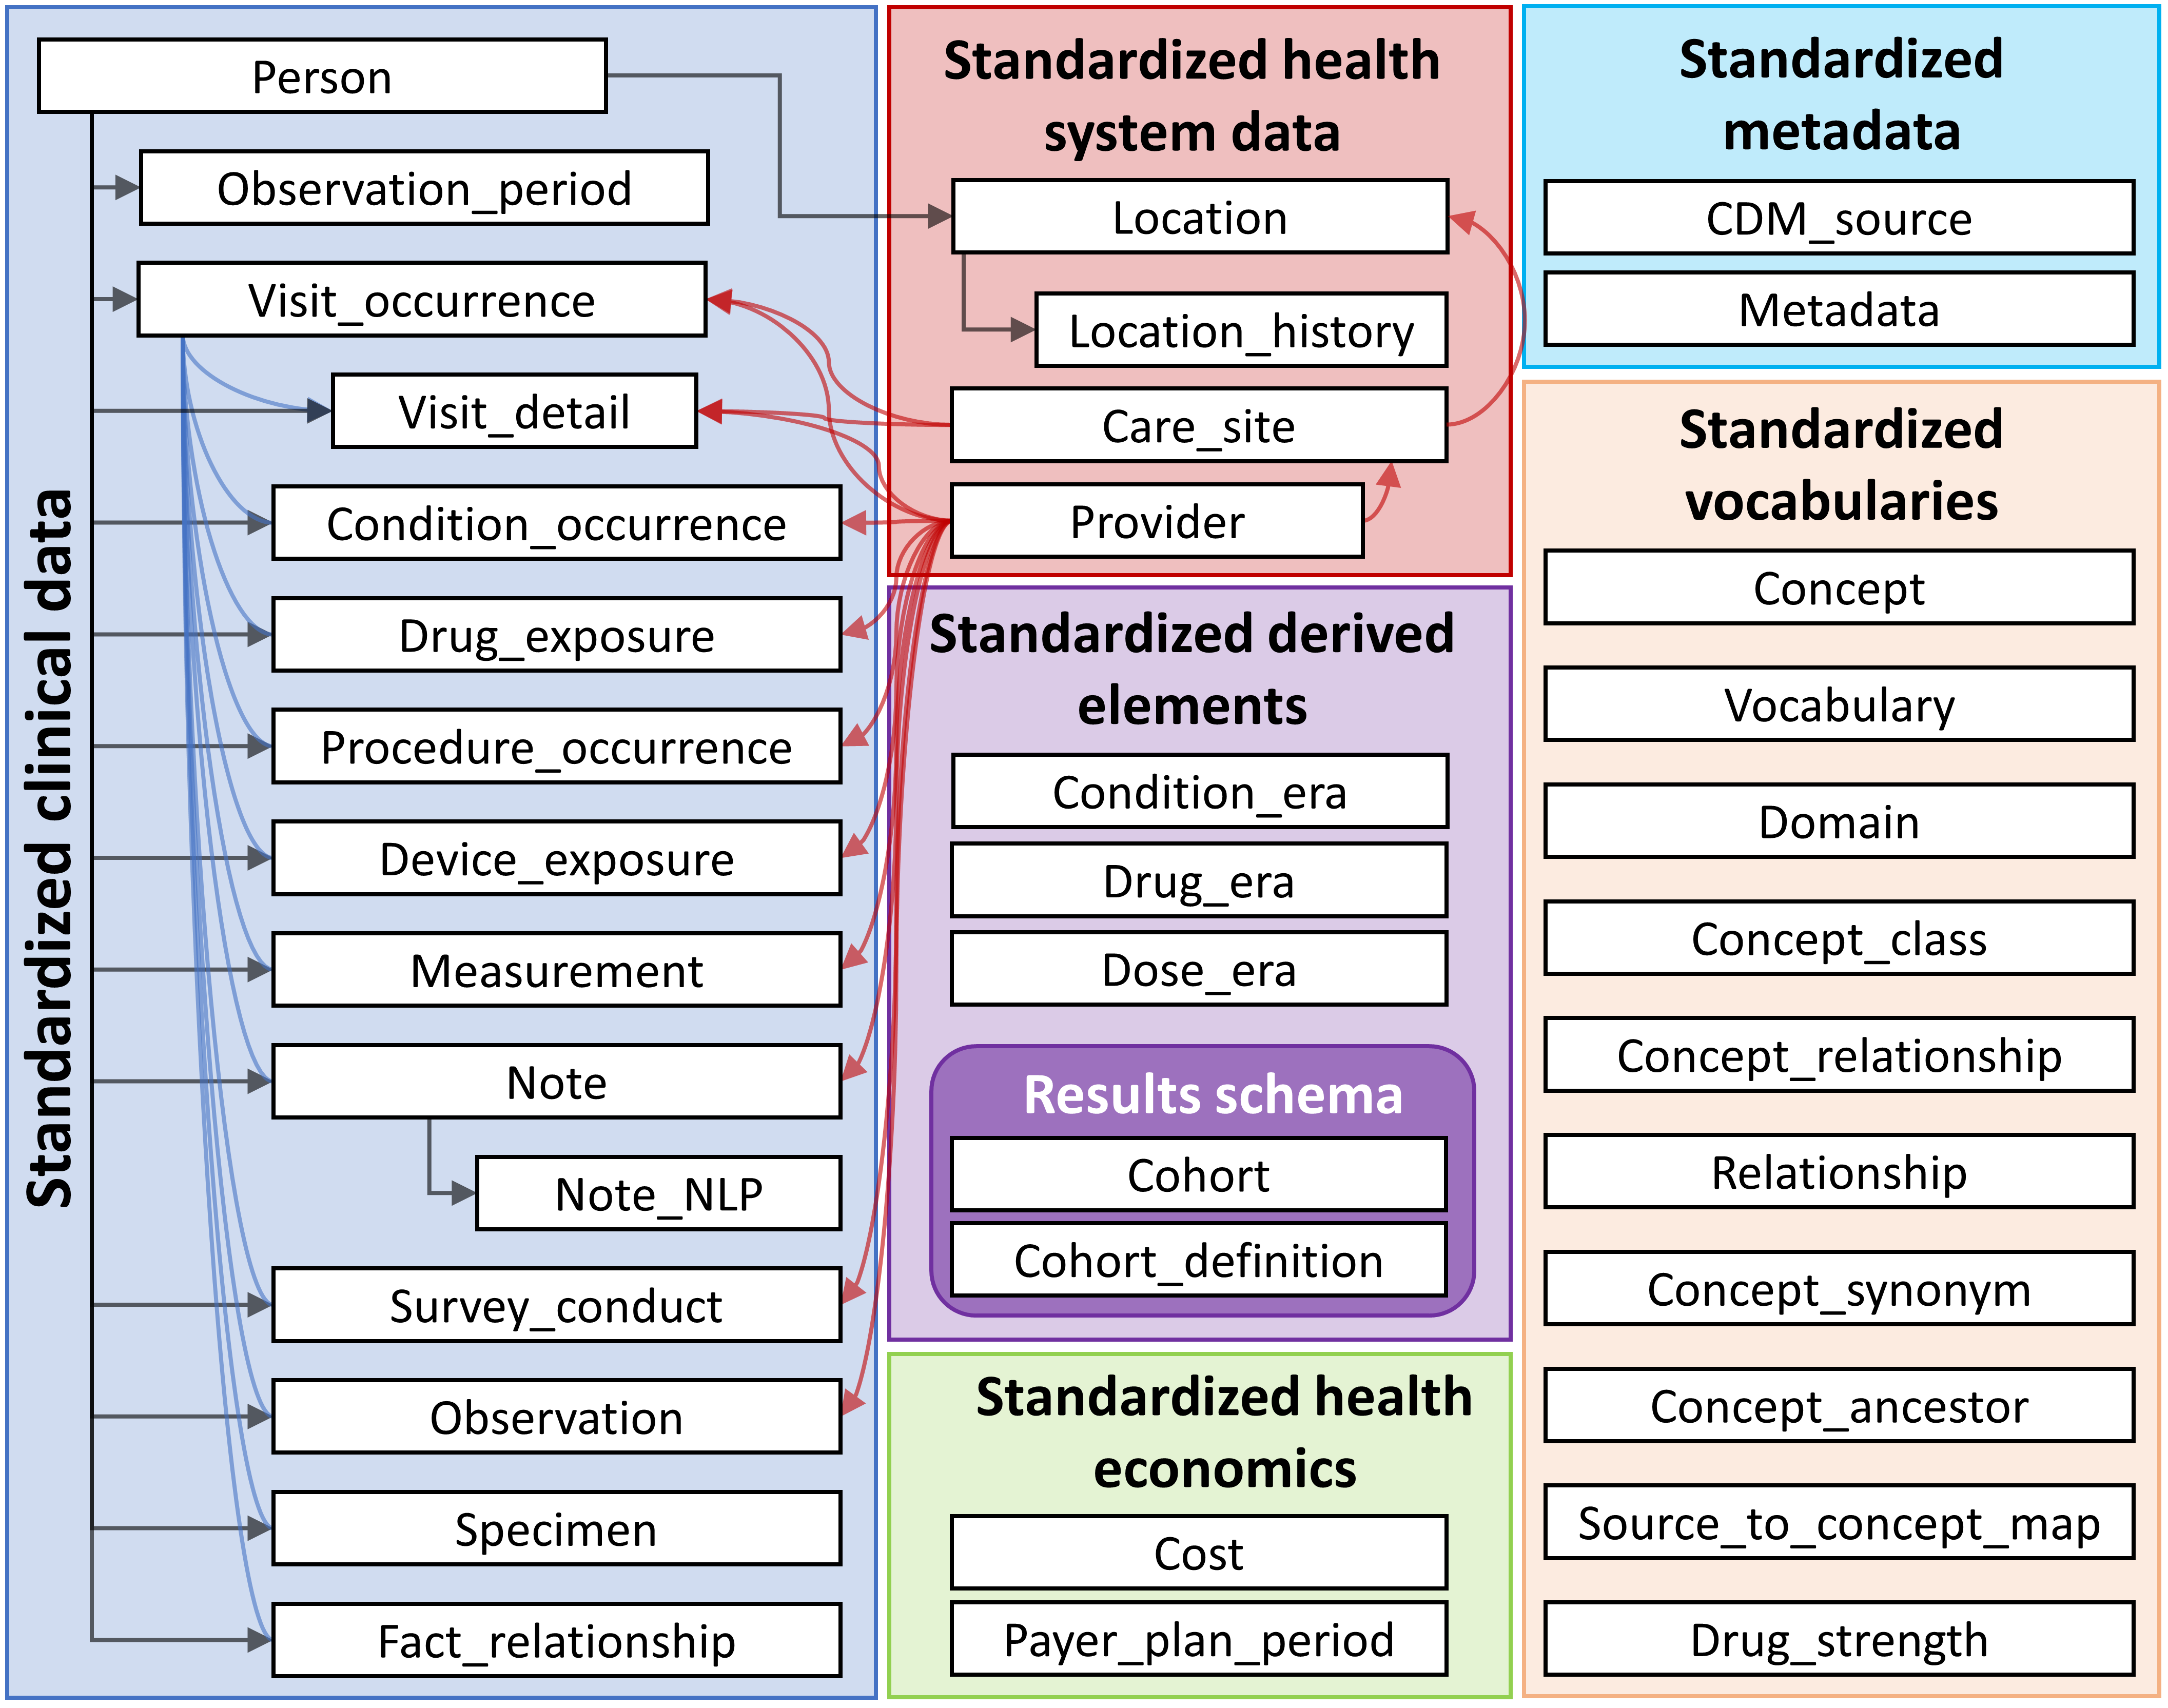
\includegraphics[width=1\linewidth]{images/CommonDataModel/cdmDiagram} \caption{CDMバージョン6.0のすべてのテーブルの概要。テーブル間のすべての関係が示されているわけではありません。}\label{fig:cdmDiagram}
\end{figure}

\section{設計原則}\label{ux8a2dux8a08ux539fux5247}

CDMは、以下の目的のために最適化されています。 \index{Common Data Model!設計原則}

\begin{itemize}
\tightlist
\item
  特定の医療介入(薬物曝露、処置、医療政策の変更など)およびアウトカム(コンディション、処置、他の薬物曝露など)を持つ患者集団を特定する。
\item
  人口統計情報、疾患の自然経過、医療提供、利用および費用、併存疾患、治療および治療の順序などさまざまなパラメータに関するこれらの患者集団の特性を評価する。
\item
  個々の患者でこれらのアウトカムが発生する可能性を予測する - 第\ref{PatientLevelPrediction}章参照。
\item
  これらの介入が集団に及ぼす影響を推定する - 第\ref{PopulationLevelEstimation}章参照。
\end{itemize}

この目標を達成するために、CDMの開発は以下のデザイン要素に従います:

\begin{itemize}
\tightlist
\item
  \textbf{目的適合性}: CDMは、医療提供者または支払者の運用ニーズを満たす目的ではなく、分析のために最適な形でデータを提供することを目指しています。 \index{Common Data Model!目的適合性}
\item
  \textbf{データ保護}: 名前や正確な誕生日など、患者の身元や保護を危うくする可能性のあるすべてのデータは限定されています。乳児の研究のために正確な誕生日が必要な場合など、研究が明示的により詳細な情報を要求する場合には例外が可能です。 \index{Common Data Model!データ保護}
\item
  \textbf{ドメインの設計}: ドメインは、各記録について人物の識別情報と日付が最低限でキャプチャされる人中心のリレーショナルデータモデルでモデル化されています。ここで、リレーショナルデータモデルとは、データが主キーおよび外部キーでリンクされたテーブルのコレクションとして表現されるものです。
\item
  \textbf{ドメインの根拠}: ドメインは、分析のユースケースがある場合(たとえばコンディション)で、そのドメインが他のものには適用されない特定の属性を持つ場合に、エンティティ-リレーションシップモデルで特定され、個別に定義されます。他のすべてのデータは、エンティティ-属性-値構造の観察テーブルに保持できます。 \index{Common Data Model!ドメイン}
\item
  \textbf{標準化されたボキャブラリ}: これらの記録の内容を標準化するために、CDMは、すべての必要かつ適切な対応する標準的な医療コンセプトを含む標準化された語彙に依存しています。
\item
  \textbf{既存のボキャブラリの再利用}: 可能な場合、これらのコンセプトは、国立医学図書館、退役軍人省、疾病予防管理センターなどの国立または業界の標準化やボキャブラリ定義組織やイニシアティブから利用されます。
\item
  \textbf{ソースコードの保持}: すべてのコードが標準化されたボキャブラリにマッピングされても、モデルは元のソースコードも保持しており、情報が失われないようにしています。 \index{Common Data Model!ソースコード} \index{Common Data Model!データ損失防止}
\item
  \textbf{技術の中立性}: CDMは特定の技術を要求しません。Oracle、SQL ServerなどのリレーショナルデータベースやSASの分析データセットなど、任意のリレーショナルデータベースで実現できます。 \index{Common Data Model!技術の中立性}
\item
  \textbf{スケーラビリティ}: CDMは、数億人の人と数十億の臨床観察を含むデータベースなど、サイズに応じてデータソースを処理および計算分析するよう最適化されています。 \index{Common Data Model!スケーラビリティ}
\item
  \textbf{後方互換性}: 以前のCDMからのすべての変更はgithubリポジトリ\href{https://github.com/OHDSI/CommonDataModel}{(https://github.com/OHDSI/CommonDataModel)}に明確に示されています。古いバージョンのCDMは現在のバージョンから簡単に作成でき、以前に存在していた情報が失われることはありません。 \index{Common Data Model!後方互換性}
\end{itemize}

\section{データモデルの規約}\label{ux30c7ux30fcux30bfux30e2ux30c7ux30ebux306eux898fux7d04}

CDMでは、暗黙的および明示的な規約がいくつか採用されています。CDMを使用して実行されるメソッドの開発者は、これらの規約を理解する必要があります。\index{共通データモデル!規約}

\subsection{モデルの一般的な規約}\label{model-Conv}

CDMは「人中心」のモデルと見なされており、すべての臨床イベントのテーブルがPERSONテーブルにリンクされています。日付または開始日と組み合わせることで、個々の人に対するすべての医療関連イベントの縦断的なビューが可能になります。この規則の例外は、さまざまなドメインのイベントに直接リンクされている標準化された医療システムデータのテーブルです。

\subsection{スキーマの一般的な規約}\label{ux30b9ux30adux30fcux30deux306eux4e00ux822cux7684ux306aux898fux7d04}

システムによってはデータベースユーザーとも呼ばれるスキーマは、読み取り専用テーブルと読み書き可能なテーブルを分けるために使用されます。臨床イベントとボキャブラリテーブルは「CDM」スキーマにあり、最終ユーザーまたは分析ツールに対して読み取り専用と見なされます。ウェブベースのツールまたはエンドユーザーによって操作する必要があるテーブルは「結果」スキーマに格納されます。「結果」スキーマ内の2つのテーブルはCOHORTおよびCOHORT\_DEFINITIONです。これらのテーブルは、ユーザーが定義する可能性のある関心のあるグループを説明するためのもので、Chapter \ref{Cohorts}に書かれています。これらのテーブルは書き込みが可能であり、実行時にCOHORTテーブルにコホートを格納できます。すべてのユーザーに対して読み書き可能なスキーマは1つだけであるため、CDMの実装方法では複数のユーザーアクセスの管理と制御が必要です。

\subsection{データテーブルの一般的な規約}\label{ux30c7ux30fcux30bfux30c6ux30fcux30d6ux30ebux306eux4e00ux822cux7684ux306aux898fux7d04}

CDMはプラットフォームに依存しません。データ型はANSI SQLデータ型(VARCHAR、INTEGER、FLOAT、DATE、DATETIME、CLOB)を用いて一般的に定義されます。VARCHARには最小必要文字列長のみが指定され、具体的なCDMのインスタンス内で拡張できます。CDMは日付および日時の形式を規定しません。CDMに対する標準クエリは、ローカルインスタンスおよび日付/日時の設定によって異なる場合があります。

\emph{注意}: データモデル自体はプラットフォームに依存しませんが、それに対応するために構築された多くのツールは特定の仕様が必要です。詳細については、Chapter \ref{OhdsiAnalyticsTools}をご覧ください。

\subsection{ドメインの一般的な規約}\label{domains}

異なる性質のイベントはドメインに整理されています。これらのイベントはドメイン固有のテーブルおよびフィールドに格納され、標準化されたボキャブラリで定義されたドメイン固有の標準コンセプトによって表現されます(セクション \ref{conceptDomains} 参照)。 各標準コンセプトには一意のドメイン割り当てがあり、そのコンセプトが記録されるテーブルを定義します。正しいドメイン割り当てはコミュニティ内で議論の余地がありますが、この厳格なドメインテーブルフィールド対応規則により、コードやコンセプトの明確な位置が常に確保されます。例えば、症状、徴候、および診断コンセプトはコンディション・ドメインに属し、CONDITION\_OCCURRENCEテーブルのCONDITION\_CONCEPT\_IDに記録されます。手順薬と呼ばれるものは通常、ソースデータの処置テーブルに処置コードとして記録されます。CDMでは、これらのレコードはDRUG\_EXPOSUREテーブルにあります。なぜなら、マッピングされた標準コンセプトが薬剤ドメインに割り当てられているからです。ドメイン数は合計30であり、テーブル\ref{tab:domains}に示されています。

表: \label{tab:domains} 各ドメインに属する標準コンセプトの数。

\begin{longtable}[]{@{}llll@{}}
\toprule\noalign{}
コンセプト数 & ドメインID & コンセプト数 & ドメインID \\
\midrule\noalign{}
\endhead
\bottomrule\noalign{}
\endlastfoot
1731378 & Drug & 183 & Route \\
477597 & Device & 180 & Currency \\
257000 & Procedure & 158 & Payer \\
163807 & Condition & 123 & Visit \\
145898 & Observation & 51 & Cost \\
89645 & Measurement & 50 & Race \\
33759 & Spec Anatomic Site & 13 & Plan Stop Reason \\
17302 & Meas Value & 11 & Plan \\
1799 & Specimen & 6 & Episode \\
1215 & Provider Specialty & 6 & Sponsor \\
1046 & Unit & 5 & Meas Value Operator \\
944 & Metadata & 3 & Spec Disease Status \\
538 & Revenue Code & 2 & Gender \\
336 & Type Concept & 2 & Ethnicity \\
194 & Relationship & 1 & Observation Type \\
\end{longtable}

\subsection{コンテンツのコンセプトによる表現}\label{ux30b3ux30f3ux30c6ux30f3ux30c4ux306eux30b3ux30f3ux30bbux30d7ux30c8ux306bux3088ux308bux8868ux73fe}

CDMデータテーブル内の各レコードのコンテンツは完全に正規化され、コンセプトを通じて表現されます。コンセプトはイベントテーブルにCONCEPT\_ID値として格納され、これはCONCEPTテーブルの外部キーです。CONCEPTテーブルは一般的な参照テーブルとして機能します。すべてのCDMインスタンスは、コンセプトの参考文献として同じCONCEPTテーブルを使用します。これにより、CDMとともにOHDSI研究ネットワークの基盤となる相互運用性の主要メカニズムが提供されます。標準コンセプトが存在しない場合や特定できない場合、CONCEPT\_IDの値は0として設定されます。これは、存在しないコンセプト、不明またはマッピング不可能な値を表します。

CONCEPTテーブルのレコードには、各コンセプトに関する詳細な情報(名前、ドメイン、クラスなど)が含まれています。コンセプト、コンセプトリレーションシップ、コンセプトの祖先など、コンセプトに関連するその他の情報は、標準化されたボキャブラリのテーブルに含まれています(Chapter \ref{StandardizedVocabularies}参照)。

\subsection{フィールドの一般的な命名規約}\label{ux30d5ux30a3ux30fcux30ebux30c9ux306eux4e00ux822cux7684ux306aux547dux540dux898fux7d04}

すべてのテーブルにわたる変数名は1つの規約に従います。

表: \label{tab:fieldConventions} フィールド名の規約。

\begin{longtable}[]{@{}
  >{\raggedright\arraybackslash}p{(\columnwidth - 2\tabcolsep) * \real{0.5000}}
  >{\raggedright\arraybackslash}p{(\columnwidth - 2\tabcolsep) * \real{0.5000}}@{}}
\toprule\noalign{}
\begin{minipage}[b]{\linewidth}\raggedright
記法
\end{minipage} & \begin{minipage}[b]{\linewidth}\raggedright
説明
\end{minipage} \\
\midrule\noalign{}
\endhead
\bottomrule\noalign{}
\endlastfoot
{[}Event{]}\_ID & 各レコードの固有識別子で、イベントテーブル間の関係を確立する外部キーとして機能します。例えば、PERSON\_IDは各個人を一意に識別します。VISIT\_OCCURRENCE\_IDは受診期間を一意に識別します。 \\
{[}Event{]}\_CONCEPT\_ID & CONCEPT参照テーブルの標準コンセプトレコードへの外部キーです。これはイベントの主要な表現として機能し、すべての標準化された分析の主要な基礎として機能します。たとえば、CONDITION\_CONCEPT\_ID = \href{http://athena.ohdsi.org/search-terms/terms/31967}{31967}には「吐き気」のSNOMEDコンセプトの参照値が含まれます。 \\
{[}Event{]}\_SOURCE\_CONCEPT\_ID & CONCEPT参照テーブルのレコードへの外部キーです。このコンセプトは、以下のソース値と等価であり、標準コンセプトである場合、それは{[}Event{]}\_CONCEPT\_IDと同一です。例えば、CONDITION\_SOURCE\_CONCEPT\_ID = \href{http://athena.ohdsi.org/search-terms/terms/45431665}{45431665}は、Read用語「吐き気」のコンセプトを示し、同様にCONDITION\_CONCEPT\_IDは標準のSNOMED-CTコンセプト\href{http://athena.ohdsi.org/search-terms/terms/31967}{31967}です。標準分析アプリケーションの場合、ソースコンセプトの使用は推奨されません。なぜなら、標準コンセプトだけがイベントの意味的内容を明確に表現し、ソースコンセプトは相互運用可能ではないためです。 \\
{[}Event{]}\_TYPE\_CONCEPT\_ID & ソース情報の出所を示す標準化されたボキャブラリ内のコンセプト参照テーブルにレコードがある外部キーです。このフィールド名にもかかわらず、これはイベントの種類やコンセプトの種類ではなく、このレコードを作成したキャプチャメカニズムを宣言します。例として、DRUG\_TYPE\_CONCEPT\_IDは、薬の記録が薬局の分配イベント(「薬局分配」)から導出されたのか、処方アプリケーション(「処方手書き」)から導出されたのかを区別します。 \\
{[}Event{]}\_SOURCE\_VALUE & ソースデータにイベントがどのように表現されているかを反映する逐語的なコードまたはフリーテキスト文字列です。これらのソース値はデータソース間で調和されていないため、標準分析アプリケーションでの使用は推奨されていません。たとえば、CONDITION\_SOURCE\_VALUEには「78702」の記録が含まれ、これはドットなしの表記で書かれたICD-9コード787.02に対応する可能性があります。 \\
\end{longtable}

\subsection{コンセプトとソース値の違い}\label{concepts-Sources}

多くのテーブルには、等価な情報が複数の場所に含まれています:ソース値、ソースコンセプト、および標準コンセプトとして。

\begin{itemize}
\tightlist
\item
  \textbf{ソース値}は、ソースデータ内のイベントレコードの元の表現です。これらは、ICD9CM、NDC、Readなどの広く使用されているコード体系のコードであり、多くの場合、パブリックドメインです。CPT4、GPI、MedDRがASCIIコード体系のコードです。これらは短い自由テキストフレーズともなり、それらは標準化されていないか管理されていないかのいずれかです。ソース値はデータテーブル内の{[}Event{]}\_SOURCE\_VALUEフィールドに格納されます。
\item
  \textbf{コンセプト}は、CDM特有のエンティティであり、臨床事実の意味を正規化します。ほとんどのコンセプトは、既存のパブリックまたは独自のコード体系に基づいていますが、その他のものは(CONCEPT\_CODEが「OMOP」で始まる)新たに作成されました。コンセプトにはすべてのドメインにまたがる一意のIDがあります。
\item
  \textbf{ソースコンセプト}は、ソースで使用されたコードを表すコンセプトです。ソースコンセプトは、既存のパブリックまたは独自のコード体系に対してのみ使用され、OMOP生成のコンセプトには使用されません。ソースコンセプトはデータテーブル内の{[}Event{]}\_SOURCE\_CONCEPT\_IDフィールドに格納されます。
\item
  \textbf{標準コンセプト}は、すべてのデータベースで臨床エンティティの意味を一意に定義するために使用されるコンセプトです。標準コンセプトは通常、既存のパブリックまたは独自の語彙ソースから引き出されます。標準コンセプトと同等の意味を持つ非標準コンセプトには、標準化されたボキャブラリで標準コンセプトへのマッピングがあります。標準コンセプトは、データ・テーブルの{[}EVENT\_SOURCE\_CONCEPT\_IDフィールドに格納されます。
\end{itemize}

ソース値は、便宜と品質保証(QA)目的でのみ提供されます。これらには、特定のデータソースの文脈のみで意味がある情報が含まれている可能性があります。ソース値およびソースコンセプトの使用はオプションですが、ソースデータがコード体系を使用している場合には\textbf{強く推奨}されます。一方、標準コンセプト用は\textbf{必須}です。この標準コンセプトの必須使用はすべてのCDMインスタンスが同じ言語を話すことを可能にします。例えば、Figure \ref{fig:pulmTubICD9} で示されているように、コンディション「肺結核」(TB)のICD9CMコードは011です。

\begin{figure}

{\centering 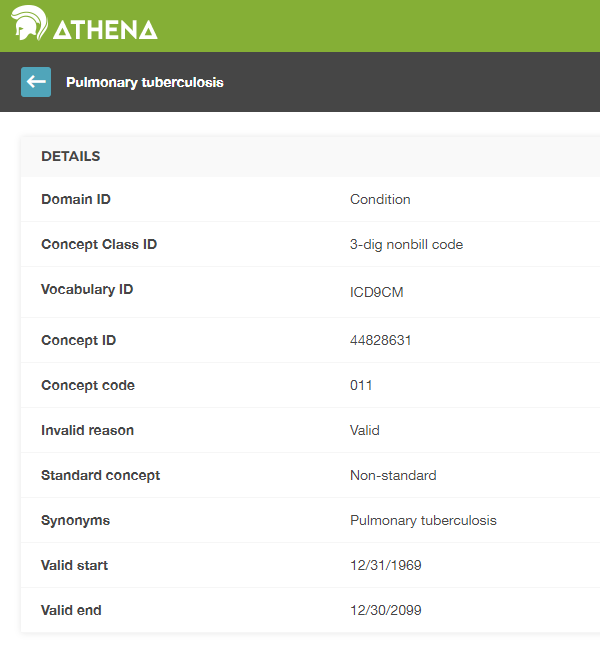
\includegraphics[width=0.75\linewidth]{images/CommonDataModel/pulmTubICD9} 

}

\caption{肺結核のICD9CMコード}\label{fig:pulmTubICD9}
\end{figure}

文脈なしにコード011を見ると、UB04語彙から「病院入院(メディケアパートAを含む)」、またはDRG語彙から「合併症、併存疾患がない神経系腫瘍」と解釈できる可能性があります。ここでコンセプトID(ソースおよび標準の両方)が役立ちます。011のICD9CMコードを表すCONCEPT\_ID値は\href{http://athena.ohdsi.org/search-terms/terms/44828631}{44828631}です。これにより、ICD9CMがUB04およびDRGから区別されます。ICD9CM TBソースコンセプトは、Figure \ref{fig:pulmTubMap} で示されるように、「非標準から標準へのマップ(OMOP)」の関係を通じて、SNOMEDボキャブラリの標準コンセプト \href{http://athena.ohdsi.org/search-terms/terms/253954}{253954}にマッピングされる。このマッピング関係は、Read、ICD10、CIEL、MeSHコードなどについても同様であるため、標準SNOMEDコンセプトを参考文献とする研究には、対応するすべてのソースコードが含まれることになる。

\begin{figure}
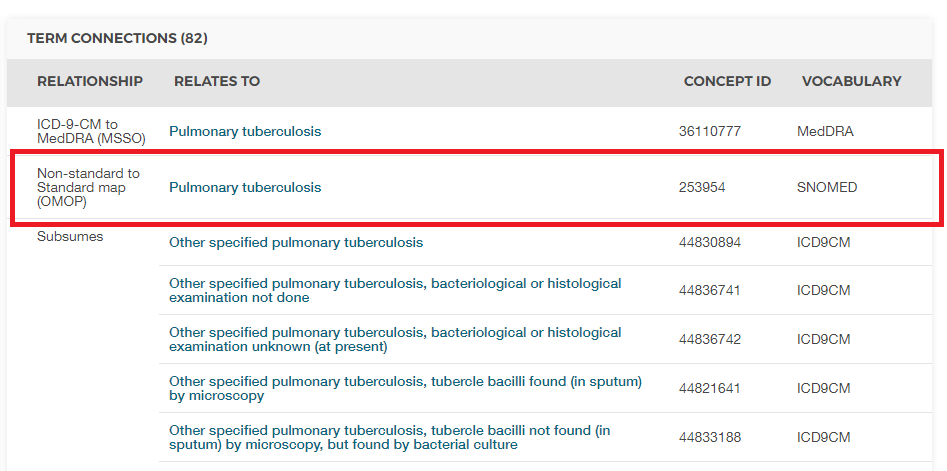
\includegraphics[width=1\linewidth]{images/CommonDataModel/pulmTubMap} \caption{肺結核のSNOMEDコード}\label{fig:pulmTubMap}
\end{figure}

標準コンセプトとソースコンセプトとの関係の例を表 \ref{tab:conditionOccurrence}に示す。

\section{CDM標準化テーブル}\label{cdmux6a19ux6e96ux5316ux30c6ux30fcux30d6ux30eb}

\index{共通データモデル!標準化テーブル}

CDMには16の臨床イベントテーブル、10のボキャブラリテーブル、2つのメタデータテーブル、4つのヘルスシステムデータテーブル、2つの医療経済データテーブル、3つの標準化された派生要素、および2つの結果スキーマテーブルが含まれています。 これらのテーブルはCDM Wikiで完全に仕様化されています \footnote{\url{https://github.com/OHDSI/CommonDataModel/wiki}}。

このテーブルが実際にどのように使用されるかを示すために、この章の残りの部分ではある1人のデータが一貫した例として使用されます。

\subsection{実行例: 子宮内膜症}\label{ux5b9fux884cux4f8b-ux5b50ux5baeux5185ux819cux75c7}

子宮内膜症は、通常女性の子宮内膜にある細胞が体の他の場所に生じる痛みを伴う状態です。重症になると、不妊症、腸や膀胱の問題を引き起こすことがあります。次のセクションでは、1人の患者のこの病気に関する体験と、それが共通データモデルでどのように表現されるかを詳述します。

\begin{center}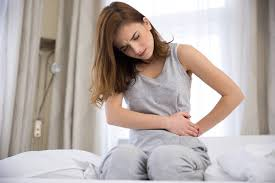
\includegraphics[width=0.5\linewidth]{images/CommonDataModel/Lauren} \end{center}

\begin{quote}
この痛みを伴う旅のすべての段階で、どれほど痛みを感じているかを皆に納得させなければなりませんでした。
\end{quote}

Laurenは何年も子宮内膜症の症状を経験していました。しかし、彼女が診断されるまでには卵巣内に嚢胞が破裂するまでかかりました。Laurenについての詳細は\url{https://endometriosis-uk.org/laurens-story} で読むことができます。

\subsection{PERSONテーブル}\label{person}

\subsubsection*{Laurenについてわかっていること}\label{laurenux306bux3064ux3044ux3066ux308fux304bux3063ux3066ux3044ux308bux3053ux3068}
\addcontentsline{toc}{subsubsection}{Laurenについてわかっていること}

\begin{itemize}
\tightlist
\item
  彼女は36歳の女性です
\item
  彼女の誕生日は1982年3月12日です
\item
  彼女は白人です
\item
  彼女はイギリス人です
\end{itemize}

これを踏まえると、彼女のPERSONテーブルは次のようになります:

\begin{longtable}[]{@{}
  >{\raggedright\arraybackslash}p{(\columnwidth - 4\tabcolsep) * \real{0.3014}}
  >{\raggedright\arraybackslash}p{(\columnwidth - 4\tabcolsep) * \real{0.1644}}
  >{\raggedright\arraybackslash}p{(\columnwidth - 4\tabcolsep) * \real{0.5342}}@{}}
\caption{\label{tab:person} PERSONテーブル。}\tabularnewline
\toprule\noalign{}
\begin{minipage}[b]{\linewidth}\raggedright
列名
\end{minipage} & \begin{minipage}[b]{\linewidth}\raggedright
値
\end{minipage} & \begin{minipage}[b]{\linewidth}\raggedright
説明
\end{minipage} \\
\midrule\noalign{}
\endfirsthead
\toprule\noalign{}
\begin{minipage}[b]{\linewidth}\raggedright
列名
\end{minipage} & \begin{minipage}[b]{\linewidth}\raggedright
値
\end{minipage} & \begin{minipage}[b]{\linewidth}\raggedright
説明
\end{minipage} \\
\midrule\noalign{}
\endhead
\bottomrule\noalign{}
\endlastfoot
PERSON\_ID & 1 & PERSON\_IDはソースから直接であれ、ビルドプロセスの一部として生成されたものであれ、整数である必要があります。 \\
GENDER\_CONCEPT\_ID & 8532 & 女性性別を参照するコンセプトIDは\href{http://athena.ohdsi.org/search-terms/terms/8532}{8532}です。 \\
YEAR\_OF\_BIRTH & 1982 & \\
MONTH\_OF\_BIRTH & 3 & \\
DAY\_OF\_BIRTH & 12 & \\
BIRTH\_DATETIME & 1982-03-12 00:00:00 & 時間が不明の場合は真夜中が使用されます。 \\
DEATH\_DATETIME & & \\
RACE\_CONCEPT\_ID & 8527 & 白人を参照するコンセプトIDは\href{http://athena.ohdsi.org/search-terms/terms/8527}{8527}です。イングリッシュエスニシティは\href{http://athena.ohdsi.org/search-terms/terms/4093769}{4093769}です。どちらも正しいですが、後者は前者に統合されます。エスニシティはRacesに一部として保存され、ETHNICITY\_CONCEPT\_IDでは保存されていません。 \\
ETHNICITY\_CONCEPT\_ ID & 38003564 & これはヒスパニックから他の人々を区別するためのUS特有の表記です。英国の場合は、エスニシティはRACE\_CONCEPT\_IDに保存されています。この場合、これは使用されません。\href{http://athena.ohdsi.org/search-terms/terms/38003564}{38003564}は「ヒスパニックではない」を表します。 \\
LOCATION\_ID & & 彼女の住所は不明です。 \\
PROVIDER\_ID & & 彼女のプライマリケア提供者は不明です。 \\
CARE\_SITE & & 彼女の主な医療施設は不明です。 \\
PERSON\_SOURCE\_ VALUE & 1 & 通常、これはソースデータでの彼女の識別子ですが、多くの場合、それはPERSON\_IDと同じです。 \\
GENDER\_SOURCE\_ VALUE & F & 実際の性別値がソースにどのように表示されるかがここに保存されます。 \\
GENDER\_SOURCE\_ CONCEPT\_ID & 0 & ソースで性別値がOHDSIが採用するコード体系でコード化されている場合、そのConceptがここに配置されます。たとえば、ソースで性別が「sex-F」と表示され、PCORNet語彙であるとされている場合、コンセプト\href{http://athena.ohdsi.org/search-terms/terms/44814665}{44814665}がこのフィールドに入ります。 \\
RACE\_SOURCE\_ VALUE & white & ソースに表示されるままの人種値がここに保存されます。 \\
RACE\_SOURCE\_ CONCEPT\_ID & 0 & 同様にGENDER\_SOURCE\_CONCEPT\_IDの原則が適用されます。 \\
ETHNICITY\_SOURCE\_ VALUE & english & ソースに表示されるままのエスニティ値がここに保存されます。 \\
ETHNICITY\_SOURCE\_ CONCEPT\_ID & 0 & 同様にGENDER\_SOURCE\_CONCEPT\_IDの原則が適用されます。 \\
\end{longtable}

\subsection{OBSERVATION\_PERIODテーブル}\label{observationPeriod}

OBSERVATION\_PERIODテーブルは、少なくとも患者の人口統計、コンディション、処置、薬剤がソースシステムで記録されている時間の範囲を定義するように設計されています。期待される感度と特異度を伴う。保険データにおいては、これは通常患者の登録期間を表します。電子健康記録(EHR)では、ほとんどの医療システムが訪問される医療機関や提供者を決定しないため、これは困難です。最善の解決策として、システムに最初に記録されたエントリを観察期間の開始日として考え、最新の記録を観察期間の終了日として考えることがよくあります。

\subsubsection*{Laurenの観察期間はどのように定義されているのですか?}\label{laurenux306eux89b3ux5bdfux671fux9593ux306fux3069ux306eux3088ux3046ux306bux5b9aux7fa9ux3055ux308cux3066ux3044ux308bux306eux3067ux3059ux304b}
\addcontentsline{toc}{subsubsection}{Laurenの観察期間はどのように定義されているのですか?}

Laurenの情報がTable \ref{tab:encounters}に示されているようにEHRシステムに記録されているとしましょう。彼女の観察期間の元となる彼女の受診は:

\begin{longtable}[]{@{}llll@{}}
\caption{\label{tab:encounters} Laurenのヘルスケアエンカウンター。}\tabularnewline
\toprule\noalign{}
エンカウンターID & 開始日 & 終了日 & タイプ \\
\midrule\noalign{}
\endfirsthead
\toprule\noalign{}
エンカウンターID & 開始日 & 終了日 & タイプ \\
\midrule\noalign{}
\endhead
\bottomrule\noalign{}
\endlastfoot
70 & 2010-01-06 & 2010-01-06 & 外来患者 \\
80 & 2011-01-06 & 2011-01-06 & 外来患者 \\
90 & 2012-01-06 & 2012-01-06 & 外来患者 \\
100 & 2013-01-07 & 2013-01-07 & 外来患者 \\
101 & 2013-01-14 & 2013-01-14 & 歩行可能 \\
102 & 2013-01-17 & 2013-01-24 & 入院患者 \\
\end{longtable}

エンカウンターレコードに基づいて彼女のOBSERVATION\_PERIODテーブルは次のようになるかもしれません:

\begin{longtable}[]{@{}
  >{\raggedright\arraybackslash}p{(\columnwidth - 4\tabcolsep) * \real{0.3151}}
  >{\raggedright\arraybackslash}p{(\columnwidth - 4\tabcolsep) * \real{0.1507}}
  >{\raggedright\arraybackslash}p{(\columnwidth - 4\tabcolsep) * \real{0.5342}}@{}}
\caption{\label{tab:observationPeriod} OBSERVATION\_PERIODテーブル。}\tabularnewline
\toprule\noalign{}
\begin{minipage}[b]{\linewidth}\raggedright
列名
\end{minipage} & \begin{minipage}[b]{\linewidth}\raggedright
値
\end{minipage} & \begin{minipage}[b]{\linewidth}\raggedright
説明
\end{minipage} \\
\midrule\noalign{}
\endfirsthead
\toprule\noalign{}
\begin{minipage}[b]{\linewidth}\raggedright
列名
\end{minipage} & \begin{minipage}[b]{\linewidth}\raggedright
値
\end{minipage} & \begin{minipage}[b]{\linewidth}\raggedright
説明
\end{minipage} \\
\midrule\noalign{}
\endhead
\bottomrule\noalign{}
\endlastfoot
OBSERVATION\_ PERIOD\_ID & 1 & これは通常、自動生成された値で、テーブル内の各レコードに一意の識別子を生成します。 \\
PERSON\_ID & 1 & これはPERSONテーブルでLauraのレコードへの外部キーであり、PERSONをOBSERVATION\_PERIODテーブルにリンクします。 \\
OBSERVATION\_PERIOD\_ START\_DATE & 2010-01-06 & これは彼女の記録された最初のエンカウンターの開始日です。 \\
OBSERVATION\_PERIOD\_ END\_DATE & 2013-01-24 & これは彼女の記録された最後のエンカウンターの終了日です。 \\
PERIOD\_TYPE\_ CONCEPT\_ID & 44814725 & 「Obs Period Type」コンセプトクラスのベストオプションは\href{http://athena.ohdsi.org/search-terms/terms/44814724}{44814724}で、「ヘルスケアエンカウンターをカバーする期間」を表します。 \\
\end{longtable}

\subsection{VISIT\_OCCURRENCE}\label{visitOccurrence}

VISIT\_OCCURRENCEテーブルは、患者の医療システムとの出会いに関する情報を保持します。OHDSIの専門用語では、これらを受診期間と呼び、個別のイベントと見なします。受診機関には12の主要カテゴリがあり、ヘルスケアが提供されるさまざまな状況を描写する広範な階層があります。最も一般的に記録される受診期間は、入院、外来、救急室および非医療機関の受診です。

\subsubsection*{Laurenのエンカウンターが受診期間としてどのように表現されるか?}\label{laurenux306eux30a8ux30f3ux30abux30a6ux30f3ux30bfux30fcux304cux53d7ux8a3aux671fux9593ux3068ux3057ux3066ux3069ux306eux3088ux3046ux306bux8868ux73feux3055ux308cux308bux304b}
\addcontentsline{toc}{subsubsection}{Laurenのエンカウンターが受診期間としてどのように表現されるか?}

例として、訪問のエンカウンターをVISIT\_OCCURRENCEテーブルで表現しましょう。

\begin{longtable}[]{@{}
  >{\raggedright\arraybackslash}p{(\columnwidth - 4\tabcolsep) * \real{0.3014}}
  >{\raggedright\arraybackslash}p{(\columnwidth - 4\tabcolsep) * \real{0.1644}}
  >{\raggedright\arraybackslash}p{(\columnwidth - 4\tabcolsep) * \real{0.5342}}@{}}
\caption{\label{tab:visitOccurrence} VISIT\_OCCURRENCEテーブル。}\tabularnewline
\toprule\noalign{}
\begin{minipage}[b]{\linewidth}\raggedright
列名
\end{minipage} & \begin{minipage}[b]{\linewidth}\raggedright
値
\end{minipage} & \begin{minipage}[b]{\linewidth}\raggedright
説明
\end{minipage} \\
\midrule\noalign{}
\endfirsthead
\toprule\noalign{}
\begin{minipage}[b]{\linewidth}\raggedright
列名
\end{minipage} & \begin{minipage}[b]{\linewidth}\raggedright
値
\end{minipage} & \begin{minipage}[b]{\linewidth}\raggedright
説明
\end{minipage} \\
\midrule\noalign{}
\endhead
\bottomrule\noalign{}
\endlastfoot
VISIT\_OCCURRENCE\_ ID & 514 & これは通常、自動生成された値で、各レコードに一意の識別子を生成します。 \\
PERSON\_ID & 1 & これはPERSONテーブルでLauraのレコードにリンクする外部キーです。 \\
VISIT\_CONCEPT\_ID & 9201 & 入院患者訪問を参照するキーは\href{http://athena.ohdsi.org/search-terms/terms/9201}{9201}です。 \\
VISIT\_START\_DATE & 2013-01-17 & 訪問の開始日です。 \\
VISIT\_START\_ DATETIME & 2013-01-17 00:00:00 & 訪問の日付と時間です。時間が不明なため、真夜中が使用されます。 \\
VISIT\_END\_DATE & 2013-01-24 & 訪問の終了日です。これは1日の訪問である場合、終了日は開始日に一致します。 \\
VISIT\_END\_DATETIME & 2013-01-24 00:00:00 & 訪問の終了日と時間です。時間が不明なため、真夜中が使用されます。 \\
VISIT\_TYPE\_ CONCEPT\_ID & 32034 & 訪問レコードの出所を示します。保険請求、病院請求、EHR記録など。これらのエンカウンターがEHRレコードに似ている例として、\href{http://athena.ohdsi.org/search-terms/terms/32035}{32035}(「EHRエンカウンターレコードから派生した訪問」)のコンセプトIDが使用されています。 \\
PROVIDER\_ID & NULL & エンカウンターレコードに提供者が関連付けられている場合、その提供者のIDがこのフィールドに入ります。これが提供者テーブルのPROVIDER\_IDフィールドの内容である必要があります。 \\
CARE\_SITE\_ID & NULL & エンカウンターレコードに関連するケアサイトがある場合、そのケアサイトのIDがこのフィールドに入ります。これがCARE\_SITEテーブルのCARE\_SITE\_IDであるべきです。 \\
VISIT\_SOURCE\_ VALUE & 入院 & 訪問値はソースでどのように表示されるかに基づいてここに入ります。Laurenのデータにはそれがありません。 \\
VISIT\_SOURCE\_ CONCEPT\_ID & NULL & 訪問値は、ソースがOHDSIによって認識されている辞書ボキャブラリを使用してコーディングされている場合、ソースコードを表すコンセプトID値がここに入ります。Laurenのデータにはそれがありません。 \\
ADMITTED\_FROM\_ CONCEPT\_ID & NULL & 既知の場合、どこから患者が入院したかを表すコンセプトが含まれます。このコンセプトは「訪問」ドメインを持つべきです。例えば、患者が自宅から病院に入院した場合には、コンセプトID \href{http://athena.ohdsi.org/search-terms/terms/8536}{8536}「自宅」が含まれます。 \\
ADMITTED\_FROM\_ SOURCE\_CONCEPT\_ID & NULL & どこから患者が入院したかを表すソース値が含まれます。上記の例では「home」です。 \\
DISCHARGE\_TO\_ CONCEPT\_ID & NULL & 既知の場合、どこに患者が退院したかを表すコンセプトが含まれます。このコンセプトは「訪問」ドメインを持つべきです。例えば、患者が介助生活施設に引き渡された場合、コンセプトID \href{http://athena.ohdsi.org/search-terms/terms/8615}{8615}「介助生活施設」が含まれます。 \\
DISCHARGE\_TO\_ SOURCE\_VALUE & NULL & どこに患者が退院したかを表すソース値が含まれます。上記の例では「Assisted living facility」です。 \\
PRECEDING\_VIS & & \\
\end{longtable}

IT\_ OCCURRENCE\_ID\textbar NULL\textbar 現在の訪問の直前の訪問を示します。ADMITTED\_FROM\_CONCEPT\_IDとは対照的に、これは実際の訪問記録をリンクし、訪問コンセプトではなくされます。また、注意すべきは後続の訪問がないことです。\textbar{}

\begin{itemize}
\tightlist
\item
  患者は1回の訪問中に複数のヘルスケア提供者と交流する可能性があり、これは特に入院の場合においてよく見られます。これらの交流はVISIT\_DETAILテーブルに記録されることができます。この章で詳しく取り上げられていませんが、VISIT\_DETAILテーブルについては詳細を\href{https://github.com/OHDSI/CommonDataModel/wiki/VISIT_DETAIL}{CDM wiki}で読むことができます。
\end{itemize}

\subsection{CONDITION\_OCCURRENCE}\label{conditionOccurrence}

CONDITION\_OCCURRENCEテーブルのレコードは、提供者によって観察されたか、患者によって報告された診断、徴候または症状を表します。

\subsubsection*{Laurenの状態は何ですか?}\label{laurenux306eux72b6ux614bux306fux4f55ux3067ux3059ux304b}
\addcontentsline{toc}{subsubsection}{Laurenの状態は何ですか?}

再度彼女のアカウントを参照すると:

\begin{quote}
約3年前、痛みを伴うことが頻繁で、規定の痛みを感じるようになりました。私の腸のすぐそばに鋭い刺すような痛みを感じ、尾骨や下骨盤の周りが触られると痛く、膨満感がありました。なので、私は月に1-2日職場を休むことがありました。鎮痛剤は時々痛みを和らげましたが、通常多くの効果はありませんでした。
\end{quote}

月経痛、別名月経困難症のSNOMEDコードは266599000です。次の表では、CONDITION\_OCCURRENCEテーブルでそれがどのように表されるかを示します。

\begin{longtable}[]{@{}
  >{\raggedright\arraybackslash}p{(\columnwidth - 4\tabcolsep) * \real{0.3014}}
  >{\raggedright\arraybackslash}p{(\columnwidth - 4\tabcolsep) * \real{0.1644}}
  >{\raggedright\arraybackslash}p{(\columnwidth - 4\tabcolsep) * \real{0.5342}}@{}}
\caption{\label{tab:conditionOccurrence} CONDITION\_OCCURRENCEテーブル。}\tabularnewline
\toprule\noalign{}
\begin{minipage}[b]{\linewidth}\raggedright
列名
\end{minipage} & \begin{minipage}[b]{\linewidth}\raggedright
値
\end{minipage} & \begin{minipage}[b]{\linewidth}\raggedright
説明
\end{minipage} \\
\midrule\noalign{}
\endfirsthead
\toprule\noalign{}
\begin{minipage}[b]{\linewidth}\raggedright
列名
\end{minipage} & \begin{minipage}[b]{\linewidth}\raggedright
値
\end{minipage} & \begin{minipage}[b]{\linewidth}\raggedright
説明
\end{minipage} \\
\midrule\noalign{}
\endhead
\bottomrule\noalign{}
\endlastfoot
CONDITION\_ OCCURRENCE\_ID & 964 & これは通常、自動生成された値で、各レコードに一意の識別子を生成します。 \\
PERSON\_ID & 1 & これはPERSONテーブルでLauraのレコードにリンクする外部キーです。 \\
CONDITION\_ CONCEPT\_ID & 194696 & SNOMEDコード266599000を表すキーは\href{http://athena.ohdsi.org/search-terms/terms/194696}{194696}です。 \\
CONDITION\_START\_ DATE & 2010-01-06 & 状態が記録された日付です。 \\
CONDITION\_START\_ DATETIME & 2010-01-06 00:00:00 & 状態が記録された日付と時間です。真夜中が使用され、時間が不明です。 \\
CONDITION\_END\_ DATE & NULL & 状態が終了したと見なされる日付ですが、これはほとんど記録されていません。 \\
CONDITION\_END\_ DATETIME & NULL & 既知の場合、状態が終了したと見なされる日付と時間です。 \\
CONDITION\_TYPE\_ CONCEPT\_ID & 32020 & この列はレコードの出所を示すことを意図しています。たとえば、保険請求、病院請求記録、EHR記録など。 \\
\end{longtable}

在資料の例には「EHRエンカウンタ診断」としてコンセプトID \href{http://athena.ohdsi.org/search-terms/terms/32020}{32020}
が使用されています。\textbar{}
\textbar CONDITION\_STATUS\_ CONCEPT\_ID\textbar NULL\textbar 既知の場合、これは周りの環境を意味します。たとえば、状態が「入院診断」などであれば、コンセプトIDが \href{http://athena.ohdsi.org/search-terms/terms/4203942}{4203942} が使用されました。\textbar{}
\textbar STOP\_REASON\textbar NULL\textbar 既知の場合、ソースデータ

\section{追加情報}\label{ux8ffdux52a0ux60c5ux5831}

この章では、CDMに存在するテーブルの一部の例を示し、データがどのように表示されるかを説明します。 詳細については、ウィキサイト\footnote{\url{https://github.com/OHDSI/CommonDataModel/wiki}}をご覧ください。

\section{まとめ}\label{ux307eux3068ux3081-2}

\begin{rmdsummary}
\begin{itemize}
\item
  CDMは広範囲の観察研究活動をサポートするように設計されています。
\item
  CDMは人中心のモデルです。
\item
  CDMはデータの構造を標準化するだけでなく、標準化されたボキャブラリを通じてコンテンツの表現も標準化します。
\item
  ソースコードは完全な追跡可能性のためにCDM内で維持されます。
\end{itemize}
\end{rmdsummary}

\section{練習問題}\label{ux7df4ux7fd2ux554fux984c}

\subsubsection*{前提条件}\label{ux524dux63d0ux6761ux4ef6}
\addcontentsline{toc}{subsubsection}{前提条件}

これらの最初の練習問題のために、以前に議論されたCDMテーブルを確認する必要があり、ATHENA\footnote{\url{http://athena.ohdsi.org/}}またはATLAS\footnote{\url{http://atlas-demo.ohdsi.org}}を通じて語彙内のコンセプトを調べる必要があります。

\begin{exercise}
\protect\hypertarget{exr:exerciseJohnPerson}{}\label{exr:exerciseJohnPerson}ジョンは1974年8月4日生まれのアフリカ系アメリカ人男性です。この情報をエンコードするPERSONテーブルのエントリを定義してください。
\end{exercise}

\begin{exercise}
\protect\hypertarget{exr:exerciseJohnOp}{}\label{exr:exerciseJohnOp}ジョンは2015年1月1日に現在の保険に加入しました。彼の保険データは2019年7月1日に抽出されました。この情報をエンコードするOBSERVATION\_PERIODテーブルのエントリを定義してください。
\end{exercise}

\begin{exercise}
\protect\hypertarget{exr:exerciseJohnDrug}{}\label{exr:exerciseJohnDrug}ジョンは2019年5月1日にイブプロフェン200 MG経口錠剤(NDCコード:76168009520)の30日分の供給を処方されました。この情報をエンコードするDRUG\_EXPOSUREテーブルのエントリを定義してください。
\end{exercise}

\subsubsection*{前提条件}\label{ux524dux63d0ux6761ux4ef6-1}
\addcontentsline{toc}{subsubsection}{前提条件}

最後の3つの課題には、セクション@ref(installR)で説明されているようにR、R-Studio、およびJavaがインストールされていることが前提となります。また、\href{https://ohdsi.github.io/SqlRender/}{SqlRender}、\href{https://ohdsi.github.io/DatabaseConnector/}{DatabaseConnector}、および\href{https://ohdsi.github.io/Eunomia/}{Eunomia}パッケージも必要で、以下のコマンドでインストールできます:

\begin{Shaded}
\begin{Highlighting}[]
\FunctionTok{install.packages}\NormalTok{(}\FunctionTok{c}\NormalTok{(}\StringTok{"SqlRender"}\NormalTok{, }\StringTok{"DatabaseConnector"}\NormalTok{, }\StringTok{"remotes"}\NormalTok{))}
\NormalTok{remotes}\SpecialCharTok{::}\FunctionTok{install\_github}\NormalTok{(}\StringTok{"ohdsi/Eunomia"}\NormalTok{, }\AttributeTok{ref =} \StringTok{"v1.0.0"}\NormalTok{)}
\end{Highlighting}
\end{Shaded}

Eunomiaパッケージは、ローカルのRセッション内で実行されるCDM内のシミュレートされたデータセットを提供します。接続の詳細は以下を使用して取得できます:

\begin{Shaded}
\begin{Highlighting}[]
\NormalTok{connectionDetails }\OtherTok{\textless{}{-}}\NormalTok{ Eunomia}\SpecialCharTok{::}\FunctionTok{getEunomiaConnectionDetails}\NormalTok{()}
\end{Highlighting}
\end{Shaded}

CDMデータベーススキーマは「main」です。これはCONDITION\_OCCURRENCEテーブルの一行を取得するためのSQLクエリの例です:

\begin{Shaded}
\begin{Highlighting}[]
\FunctionTok{library}\NormalTok{(DatabaseConnector)}
\NormalTok{connection }\OtherTok{\textless{}{-}} \FunctionTok{connect}\NormalTok{(connectionDetails)}
\NormalTok{sql }\OtherTok{\textless{}{-}} \StringTok{"SELECT *}
\StringTok{FROM @cdm.condition\_occurrence}
\StringTok{LIMIT 1;"}
\NormalTok{result }\OtherTok{\textless{}{-}} \FunctionTok{renderTranslateQuerySql}\NormalTok{(connection, sql, }\AttributeTok{cdm =} \StringTok{"main"}\NormalTok{)}
\end{Highlighting}
\end{Shaded}

\begin{exercise}
\protect\hypertarget{exr:exerciseGiBleedRecords}{}\label{exr:exerciseGiBleedRecords}SQLとRを使用して、「消化管出血」(コンセプトID\href{http://athena.ohdsi.org/search-terms/terms/192671}{192671})のすべてのレコードを取得してください。
\end{exercise}

\begin{exercise}
\protect\hypertarget{exr:exercisePersonSource}{}\label{exr:exercisePersonSource}SQLとRを使用して、ソースコードを使用して「消化管出血」のすべてのレコードを取得してください。このデータベースはICD-10を使用しており、関連するICD-10コードは「K92.2」です。
\end{exercise}

\begin{exercise}
\protect\hypertarget{exr:exercisePerson61Records}{}\label{exr:exercisePerson61Records}SQLとRを使用して、PERSON\_ID 61の人物の観察期間を取得してください。
\end{exercise}

提案される答えは付録@ref(Cdmanswers)にあります。

\chapter{第5章 --翻訳作業中-- 標準化ボキャブラリ}\label{StandardizedVocabularies}

\index{standardized vocabularies}

\emph{章の著者: Christian Reich \& Anna Ostropolets}

OMOPで標準化されたボキャブラリ、しばしば単に「ボキャブラリ」と呼ばれるものは、OHDSI研究ネットワークの基礎部分であり、共通データモデル(CDM)の不可欠な部分です。これにより、データの内容を定義して方法論、定義、結果の標準化を可能にし、本当の遠隔(ファイアウォールの背後)ネットワーク研究と分析への道を開きます。通常、観察医療データの内容を見つけて解釈することは、研究者が数多くの異なる方法で臨床イベントを説明するのに対処しなければならない状態に置かれます。OHDSIは標準化された形式だけでなく、厳密な標準コンテンツへの統合も必要とします。

この章では、まず標準化されたボキャブラリの主要な原則、その構成要素、およびそれを理解し利用するために必要な関連する規則、慣例、および典型的な状況について説明します。また、継続的な改善のためにコミュニティの支援が必要な箇所も指摘します。

\section{なぜボキャブラリが必要で、なぜ標準化が必要か}\label{ux306aux305cux30dcux30adux30e3ux30d6ux30e9ux30eaux304cux5fc5ux8981ux3067ux306aux305cux6a19ux6e96ux5316ux304cux5fc5ux8981ux304b}

医学ボキャブラリの歴史は、中世のロンドンでペストやその他の疾患の流行を管理するために作成された死亡報告書(「Bill of Mortality」)に遡ります(図\ref{fig:bill}参照)。\index{Bill of Mortality}

\begin{figure}

{\centering 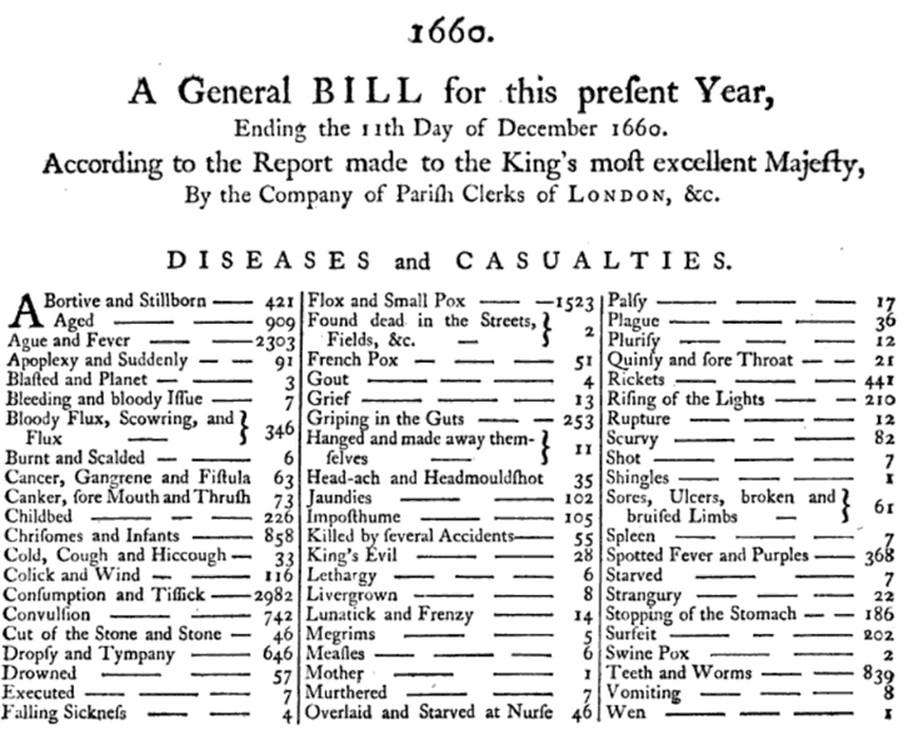
\includegraphics[width=1\linewidth]{images/StandardizedVocabularies/bill} 

}

\caption{1660年のロンドン死亡報告書には、その時代に知られていた62の疾患の分類システムを使用して住民の死因が示されています。}\label{fig:bill}
\end{figure}

それ以来、分類は大幅に拡大し、医療の他の側面、例えば処置やサービス、薬剤、医療デバイスなどにも広がりました。主な原則は変わっていません:それらは患者データを収集、分類、分析するためにいくつかの医療コミュニティが合意した制御されたボキャブラリ、専門用語、階層またはオントロジーです。これらの多くのボキャブラリは、公的および政府機関によって長期的に管理されます。例えば、世界保健機関(WHO)は最近第11版(ICD11)が追加された「国際疾病分類(ICD)」を作成しています。各国の政府は、ICD10CM(米国)、ICD10GM(ドイツ)などの国別バージョンを作成します。政府はまた、薬品のマーケティングと販売を管理し、認証された薬剤の国家リポジトリを維持します。ボキャブラリはまた、電子健康記録(EHR)システムや医療保険の請求報告のために、商業製品または内部使用としてプライベートセクターでも使用されます。

その結果、各国、地域、医療システムおよび施設は、その使用場所でのみ関連するであろう独自の分類を持っています。この多様なボキャブラリシステムは、それらが使用されるシステムの相互運用性を防ぎます。標準化は患者データの交換を可能にし、グローバルレベルでの健康データ分析を解き放ち、性能の特性評価および品質評価を含む体系的かつ標準化された研究を可能にする鍵です。この問題に対処するために、多国籍組織が誕生し、広範な基準を作成し始めました。例えば、前述のWHOや、「標準医療用語(SNOMED)」や「論理的観察識別子名とコード(LOINC)」です。米国では、健康IT基準委員会(HITAC)は、全国的な異なる組織間での健康情報交換の共通プラットフォームとしてSNOMED、LOINC、および薬品ボキャブラリRxNormの使用を国家健康IT調整官(ONC)に推奨しています。

OHDSIは、観察研究のためのグローバルスタンダードであるOMOP CDMを開発しました。CDMの一部として、OMOPで標準化されたボキャブラリは次の2つの主要な目的のために利用可能です:

\begin{itemize}
\tightlist
\item
  コミュニティで使用されるすべてのボキャブラリの共通リポジトリ
\item
  研究での使用のための標準化とマッピング
\end{itemize}

標準化されたボキャブラリは無料でコミュニティに提供されており、OMOP CDMインスタンスには必須の参考文献テーブルとして\textbf{使用しなければなりません}。

\subsection{標準化されたボキャブラリの構築}\label{ux6a19ux6e96ux5316ux3055ux308cux305fux30dcux30adux30e3ux30d6ux30e9ux30eaux306eux69cbux7bc9}

標準化されたボキャブラリのすべてのボキャブラリは、共通の形式に統合されています。これにより、研究者が元のボキャブラリの複数の異なる形式とライフサイクルの慣例を理解して扱う必要がなくなります。すべてのボキャブラリは定期的に更新され、Pallasシステムを使用して統合されます\footnote{\url{https://github.com/OHDSI/Vocabulary-v5.0}}。これは、全体のOMOP CDMワークグループの一部であるOHDSIボキャブラリチームによって構築および運営されています。誤りを見つけた場合は、OHDSIフォーラム\footnote{\url{https://forums.ohdsi.org}}またはCDM GitHubページ\footnote{\url{https://github.com/OHDSI/CommonDataModel/issues}}に投稿して、私たちのリソースを改善するのにご協力ください。 \index{Pallas system}

\subsection{標準化されたボキャブラリへのアクセス}\label{accessVocabularies}

標準化されたボキャブラリを取得するためには、自分でPallasを実行する必要はありません。代わりに、ATHENA\footnote{\url{http://athena.ohdsi.org}}から最新バージョンをダウンロードし、ローカルデータベースにロードできます。ATHENAでは、ボキャブラリのファセット検索も可能です。 \index{ATHENA} \index{standardized vocabularies!download} \index{standardized vocabularies!search}

OMOP CDMのボキャブラリをすべて選んで、標準化されたボキャブラリテーブルのすべてを含むzipファイルをダウンロードします。標準コンセプトを持つボキャブラリ(セクション\ref{standardConcepts}参照)と非常に一般的な使用法は事前に選択されています。提供元データで使用されているボキャブラリを追加します。著作権のあるボキャブラリには選択ボタンがありません。「ライセンス必要」ボタンをクリックしてそのようなボキャブラリをリストに組み込みます。ボキャブラリチームが連絡し、ライセンスの証明を示すか、適切な人々と連絡を取り合うためのサポートを提供します。

\subsection{ボキャブラリの元: 採用するか構築するか}\label{ux30dcux30adux30e3ux30d6ux30e9ux30eaux306eux5143-ux63a1ux7528ux3059ux308bux304bux69cbux7bc9ux3059ux308bux304b}

OHDSIは一般的に、既存のボキャブラリを採用することを優先します。なぜなら、(i)多くのボキャブラリがコミュニティ内で観察データに使用されているため、(ii)ボキャブラリの構築とメンテナンスは複雑で、成熟するためには多くの利害関係者の長期にわたる協力が必要だからです。この理由から、特定の組織がボキャブラリを提供しており、それらは生成、廃止、統合および分割のライフサイクルに従います(セクション\ref{conceptLifeCycle}参照)。現在、OHDSIは条件タイプコンセプト(例:コンディションタイプコンセプト)などの内部管理ボキャブラリのみを作成しています。唯一の例外は、アメリカ以外でのみ使用される薬剤をカバーするRxNorm Extensionボキャブラリです(セクション\ref{rxNormExtension}参照)。

\section{コンセプト}\label{ux30b3ux30f3ux30bbux30d7ux30c8}

OMOP CDMのすべての臨床イベントはコンセプトとして表現され、それぞれのイベントのセマンティックな意味を表します。これらはデータレコードの基本的な構成要素であり、ほとんどすべてのテーブルが完全に正規化されています(一部の例外を除く)。コンセプトはCONCEPTテーブルに格納されます(図\ref{fig:concept}を参照)。\index{concept}

\begin{figure}

{\centering 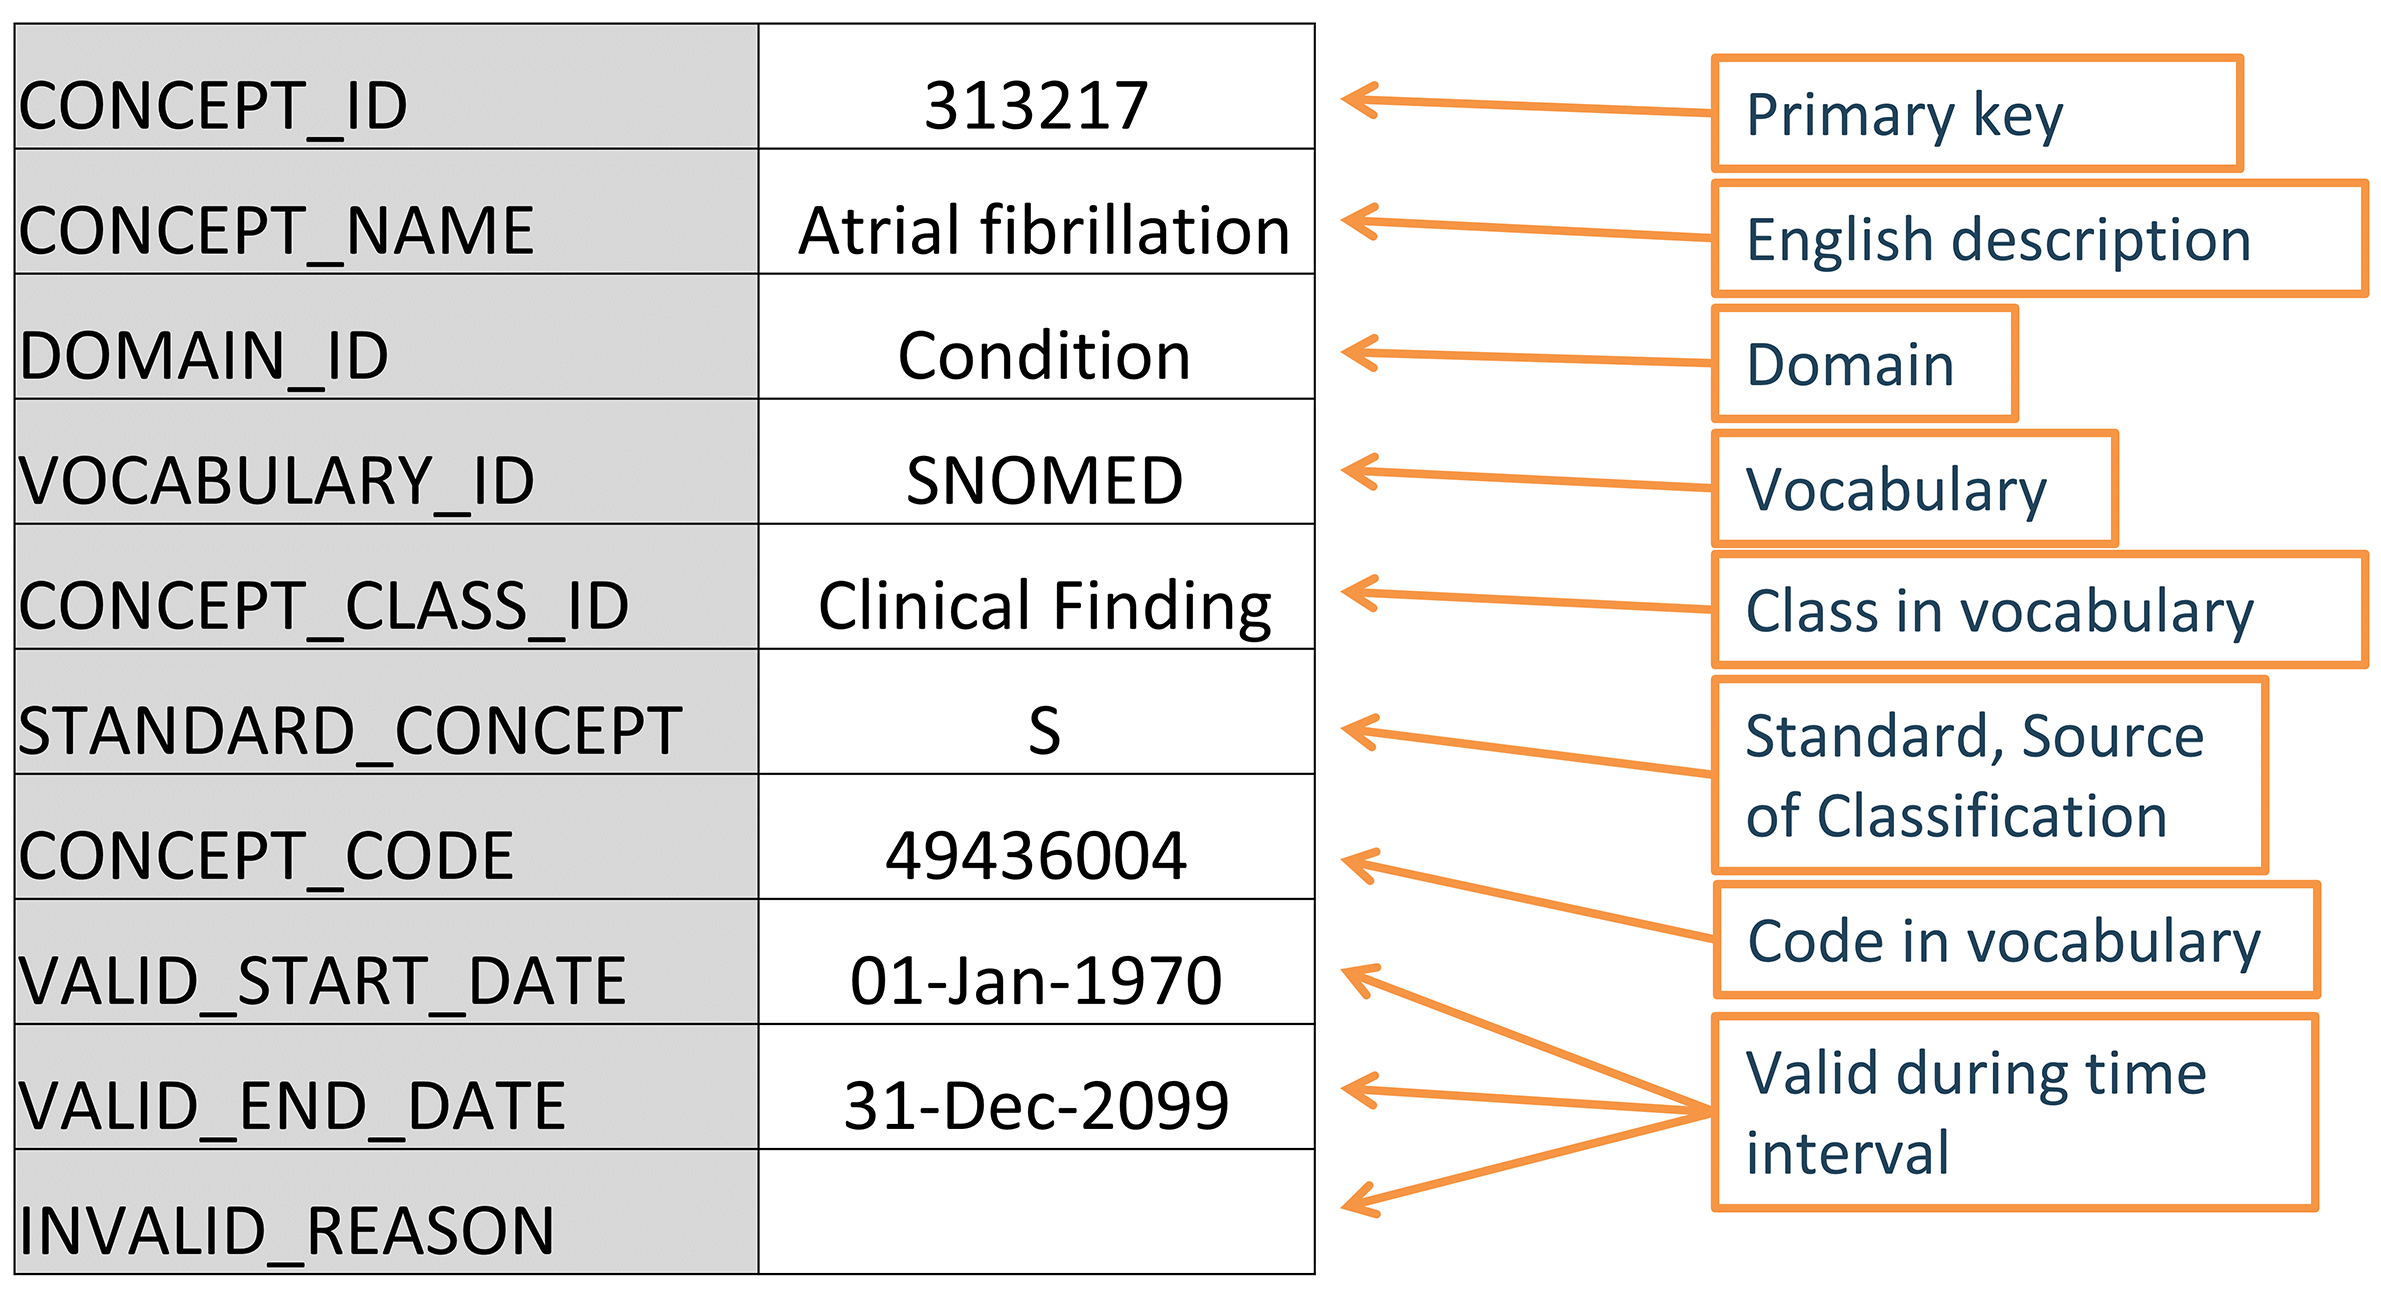
\includegraphics[width=0.9\linewidth]{images/StandardizedVocabularies/concept} 

}

\caption{OMOP CDMにおける標準化されたボキャブラリコンセプトの標準的な表現。提供されている例は心房細動のSNOMEDコードに対するCONCEPTテーブルのレコードです。}\label{fig:concept}
\end{figure}

このシステムは\textbf{包括的}であることを意味し、患者の医療体験に関連するすべてのイベント(例:疾患、手続き、薬剤の曝露など)や医療システムの一部の管理情報(例:受診期間、ケア施設など)をカバーするのに十分なコンセプトが存在します。

\subsection{コンセプトID}\label{ux30b3ux30f3ux30bbux30d7ux30c8id}

各コンセプトにはプライマリキーとして使用されるコンセプトIDが割り当てられます。この無意味な整数IDは、CDMのイベントテーブルにデータを記録する際に使用され、元のボキャブラリコードではありません。 \index{concept!identifier}

\subsection{コンセプト名}\label{ux30b3ux30f3ux30bbux30d7ux30c8ux540d}

各コンセプトには1つの名前があります。名前は常に英語で、ボキャブラリのソースからインポートされます。ソースボキャブラリに複数の名前がある場合、最も表現力のあるものが選択され、残りはCONCEPT\_SYNONYMテーブルに同じCONCEPT\_IDキーで保存されます。非英語の名前もCONCEPT\_SYNONYMに記録され、LANGUAGE\_CONCEPT\_IDフィールドに適切な言語コンセプトIDが格納されます。名前は255文字までとされており、非常に長い名前は切り捨てられ、フルレングスバージョンが別のシノニムとして記録され、最大1000文字まで保存できます。

\subsection{ドメイン}\label{conceptDomains}

各コンセプトにはDOMAIN\_IDフィールドにドメインが割り当てられています。これは数値のCONCEPT\_IDとは対照的に、ドメインに対する短い大文字小文字区別のない一意の英数字IDです。例として、「Condition」、「Drug」、「Procedure」、「Visit」、「Device」、「Specimen」などのドメイン識別子があります。曖昧または事前コード化された(組み合わせ)コンセプトは複合ドメインに属することがありますが、標準コンセプト(セクション\ref{standardConcepts}参照)は常に単一のドメインに割り当てられます。ドメインはまた、臨床イベントまたはイベント属性がCDMテーブルおよびフィールドのどこに記録されるかを指示します。
ドメインの割り当ては、\href{https://github.com/ohDSI/vocabulary-v5.0}{Pallas}に示されているヒューリスティックを使用してボキャブラリの取り込み中に行われるOMOP固有の機能です。ソースボキャブラリは、さまざまな程度で混合ドメインのコードを組み合わせる傾向があります(図\ref{fig:domains}参照)。\index{domain!concept}

\begin{figure}

{\centering 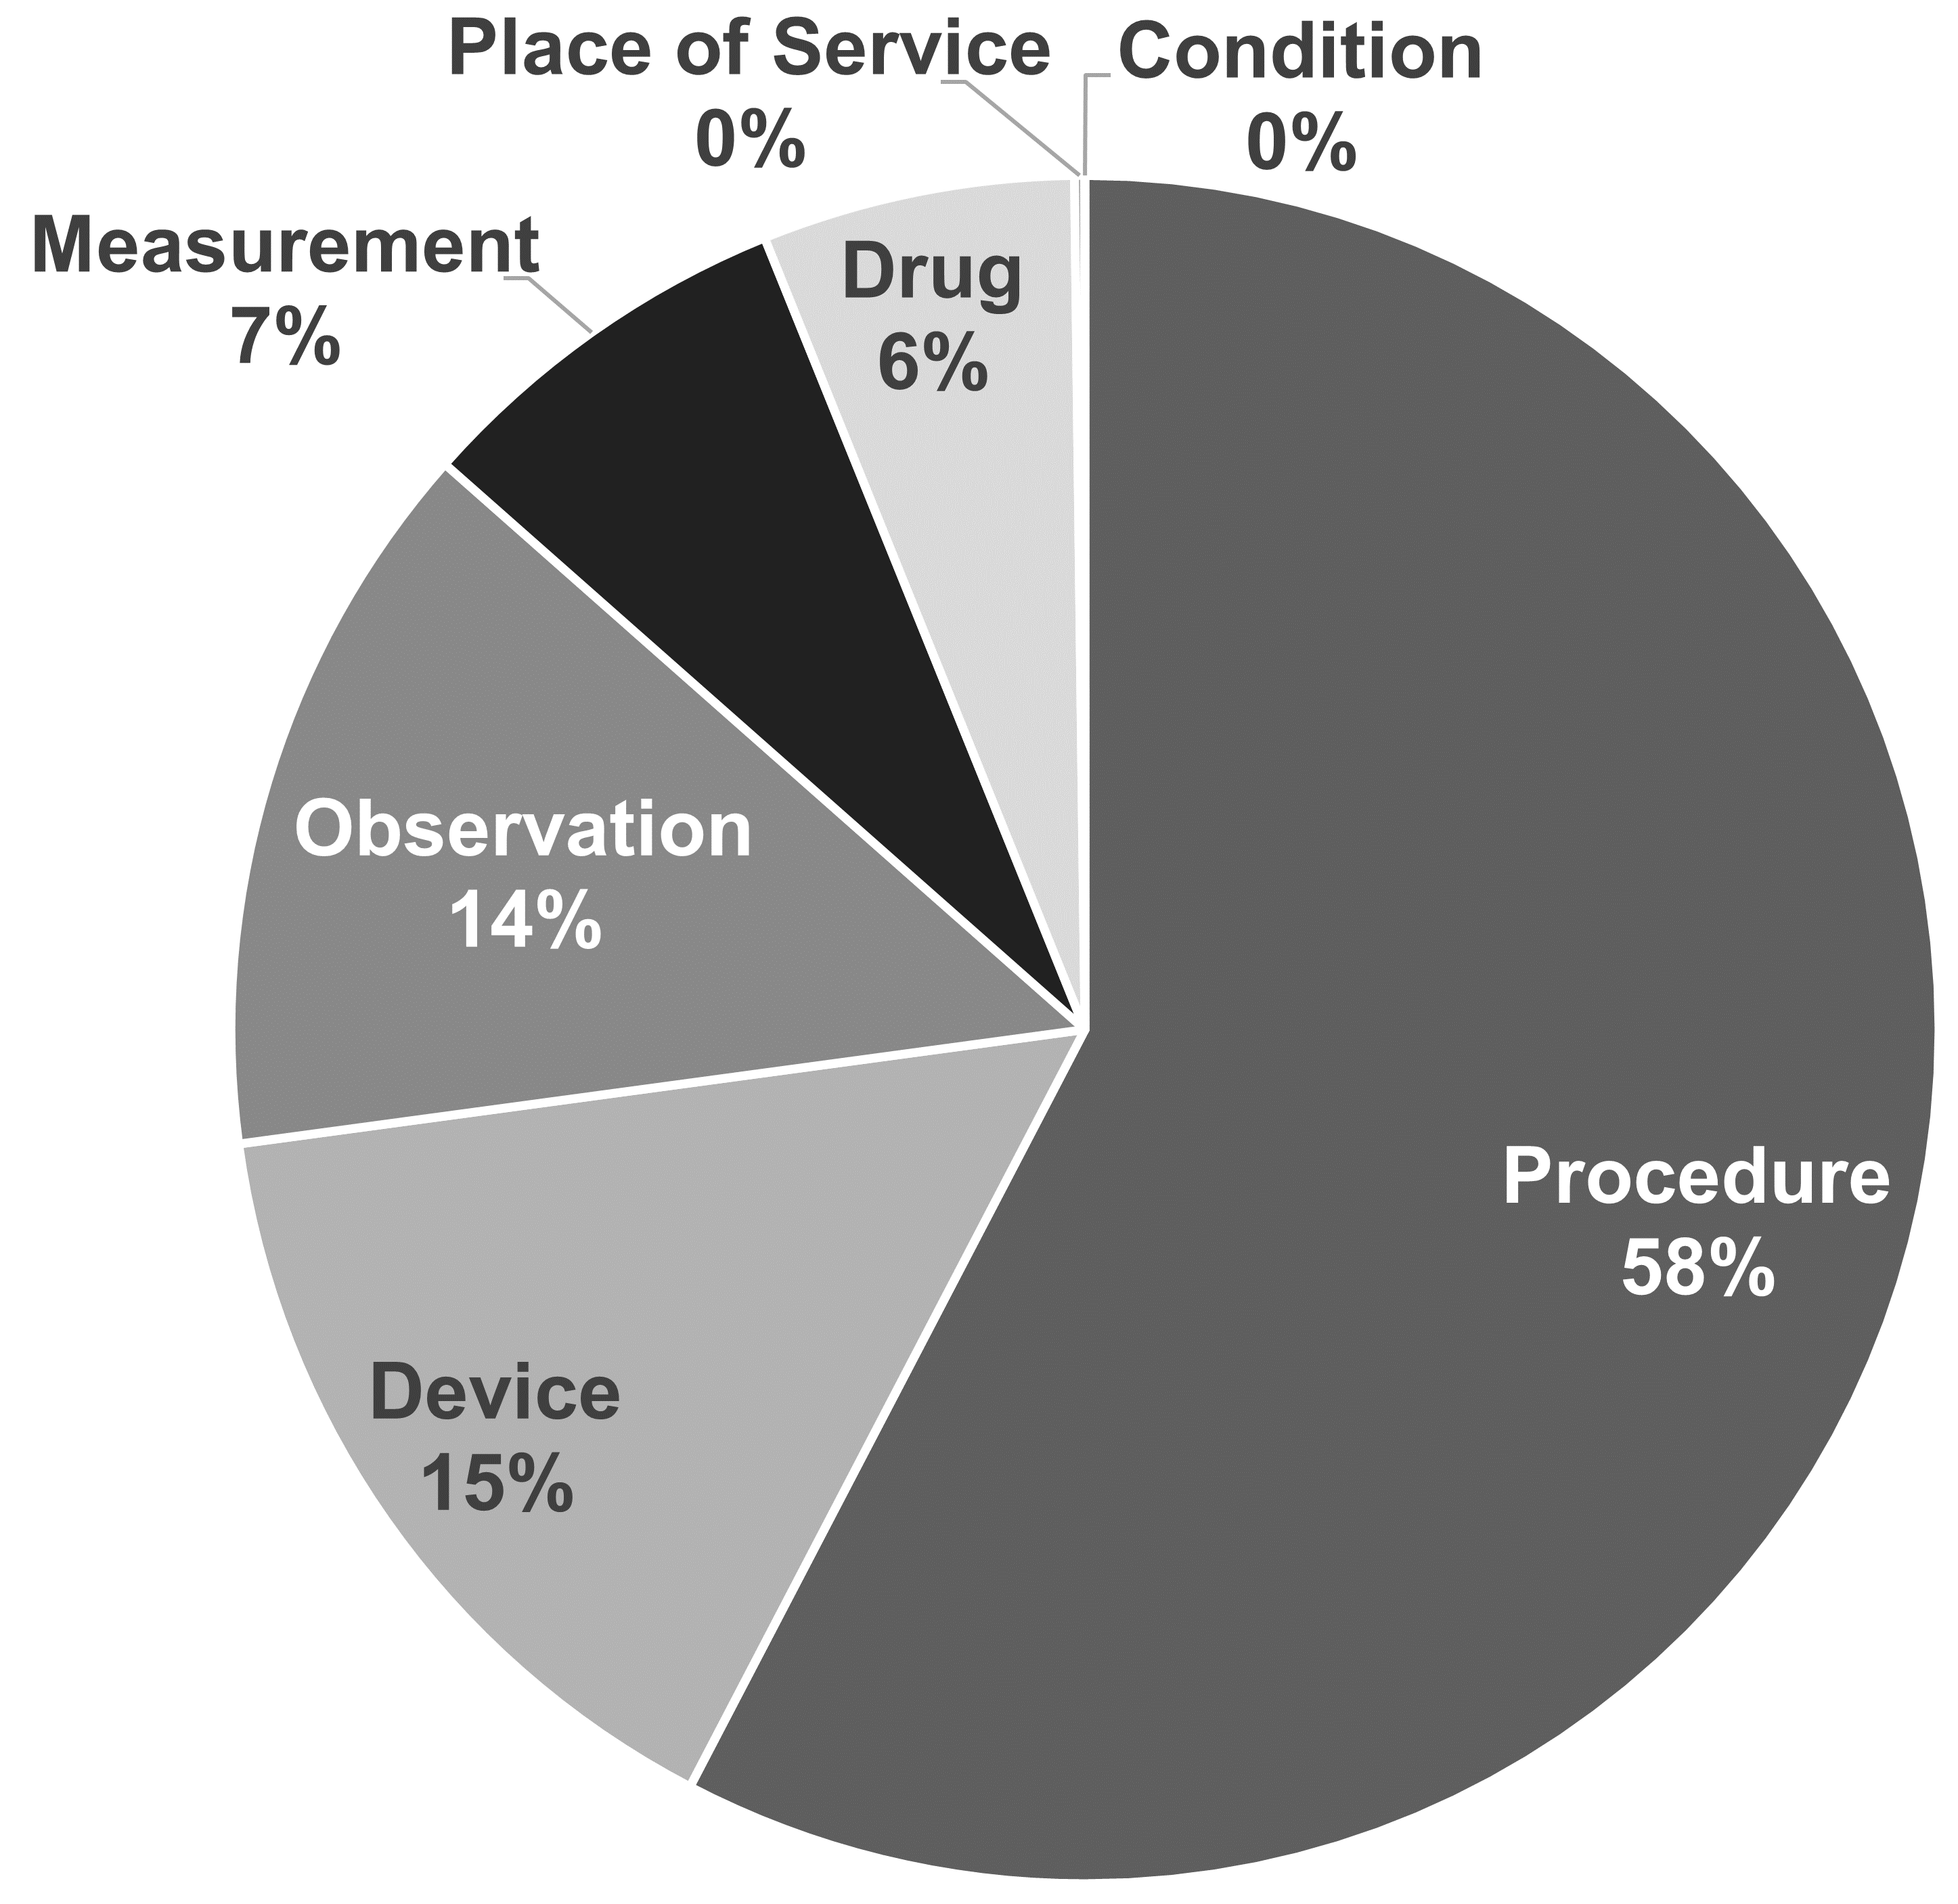
\includegraphics[width=0.7\linewidth]{images/StandardizedVocabularies/domains} 

}

\caption{手続きボキャブラリCPT4およびHCPCSにおけるドメインの割り当て。直感的には、これらのボキャブラリは単一のドメインのコードとコンセプトを含むべきですが、実際には混在しています。}\label{fig:domains}
\end{figure}

ドメインのヒューリスティックは、ドメインの定義に従います。これらの定義はCDMのテーブルおよびフィールド定義から派生しています(Chapter \ref{CommonDataModel}参照)。ヒューリスティックは完全ではなく、グレーゾーンも存在します(セクション\ref{specialSituations}「特別な状況」参照)。ドメインが誤って割り当てられているコンセプトを見つけた場合、\href{https://forums.ohdsi.org}{フォーラム}または\href{https://github.com/OHDSI/CommonDataModel/issues}{CDM問題}の投稿を通じて報告し、プロセスの改善に貢献してください。

\subsection{ボキャブラリ}\label{ux30dcux30adux30e3ux30d6ux30e9ux30ea}

各ボキャブラリには短い大文字小文字区別のない一意の英数字IDが付けられており、通常はボキャブラリの省略名を使用し、ダッシュを省略します。たとえば、ICD-9-CMは「ICD9CM」のボキャブラリIDを持ちます。現在、OHDSIがサポートしているボキャブラリは111あり、そのうち78は外部ソースから採用されており、残りはOMOP内部のボキャブラリです。これらのボキャブラリは通常、四半期ごとに更新されます。ボキャブラリのソースとバージョンはVOCABULARY参照ファイルで定義されています。 \index{vocabulary}

\subsection{コンセプトクラス}\label{ux30b3ux30f3ux30bbux30d7ux30c8ux30afux30e9ux30b9}

一部のボキャブラリはコードまたはコンセプトを分類しており、それを大文字小文字区別のない一意の英数字IDで示します。たとえば、SNOMEDには「意味タグ」と呼ばれる33のコンセプトクラスがあり、臨床所見、社会的状況、身体構造などがあります。これらはコンセプトの垂直的な区分です。また、MedDRAやRxNormのように、階層的な階層の横方向のレベルを分類するコンセプトクラスを持つものもあります。コンセプトクラスを持たないボキャブラリ(例えばHCPCS)の場合、ボキャブラリIDがConcept Class IDとして使用されます。 \index{concept!class}

表: \label{tab:sublassification} コンセプトクラスにおける水平および垂直のサブ分類原則を持つボキャブラリと持たないボキャブラリ。

\begin{longtable}[]{@{}
  >{\raggedright\arraybackslash}p{(\columnwidth - 2\tabcolsep) * \real{0.2045}}
  >{\raggedright\arraybackslash}p{(\columnwidth - 2\tabcolsep) * \real{0.7955}}@{}}
\toprule\noalign{}
\begin{minipage}[b]{\linewidth}\raggedright
コンセプトクラスの区分原則
\end{minipage} & \begin{minipage}[b]{\linewidth}\raggedright
ボキャブラリ
\end{minipage} \\
\midrule\noalign{}
\endhead
\bottomrule\noalign{}
\endlastfoot
水平 & すべての薬物ボキャブラリ、ATC、CDT、Episode、HCPCS、HemOnc、ICDs、MedDRA、OSM、国勢調査 \\
垂直 & CIEL、HES専門、ICDO3、MeSH、NAACCR、NDFRT、OPCS4、PCORNET、Plan、PPI、Provider、SNOMED、SPL、UCUM \\
混在 & CPT4、ISBT、LOINC \\
なし & APC、すべてのタイプコンセプト、民族性、OXMIS、種族、収益コード、スポンサー、供給者、UB04、訪問 \\
\end{longtable}

水平コンセプトクラスにより、特定の階層レベルを決定することができます。たとえば、薬物ボキャブラリRxNormにおけるコンセプトクラス「Ingredient」は階層の最上位レベルを定義します。垂直モデルでは、コンセプトクラスのメンバーは最上位から最下位までの任意の階層レベルであることができます。

\subsection{標準コンセプト}\label{standardConcepts}

各臨床イベントを表す1つのコンセプトが標準として指定されます。たとえば、コンディションドメインにおいて、「心房細動」を定義するMESHコードD001281、CIELコード148203、SNOMEDコード49436004、ICD9CMコード427.31、およびReadコードG573000のすべてがSNOMEDコンセプトは標準であり、この条件をデータ内で表します。他のものは非標準またはソースコンセプトとして指定され、標準のものにマッピングされています。標準コンセプトはSTANDARD\_CONCEPTフィールドに「S」で示されます。そして、これらの標準コンセプトのみが''\_CONCEPT\_ID''で終わるCDMフィールドにデータを記録するために使用されます。 \index{standard concept}

\subsection{非標準コンセプト}\label{ux975eux6a19ux6e96ux30b3ux30f3ux30bbux30d7ux30c8}

非標準コンセプトは臨床イベントを表現するためには使用されませんが、標準化されたボキャブラリの一部であり、ソースデータに頻繁に見られます。そのため、それらは「ソースコンセプト」とも呼ばれます。ソースコンセプトを標準コンセプトに変換するプロセスは「マッピング」と呼ばれます(セクション@ref(コンセプトMapping)参照)。非標準コンセプトにはSTANDARD\_CONCEPTフィールドに値がありません(NULL)。

\subsection{分類コンセプト}\label{ux5206ux985eux30b3ux30f3ux30bbux30d7ux30c8}

これらのコンセプトは標準ではなく、したがってデータを表現するためには使用されませんが、標準コンセプトと階層的に関連しており、そのため階層クエリを実行するために使用できます。たとえば、MedDRAコード10037908のすべての子孫をクエリする場合(MedDRAライセンスを取得していないユーザーには表示されません。アクセス制限についてはセクション\ref{accessVocabularies}参照)では、標準のSNOMEDコンセプト「心房細動」を取得します(CONCEPT\_ANCESTORテーブルを使用した階層クエリについてはセクション\ref{conceptAncestor}を参照) - 図\ref{fig:hierarchy}を参照。 \index{classification concept}

\begin{figure}

{\centering 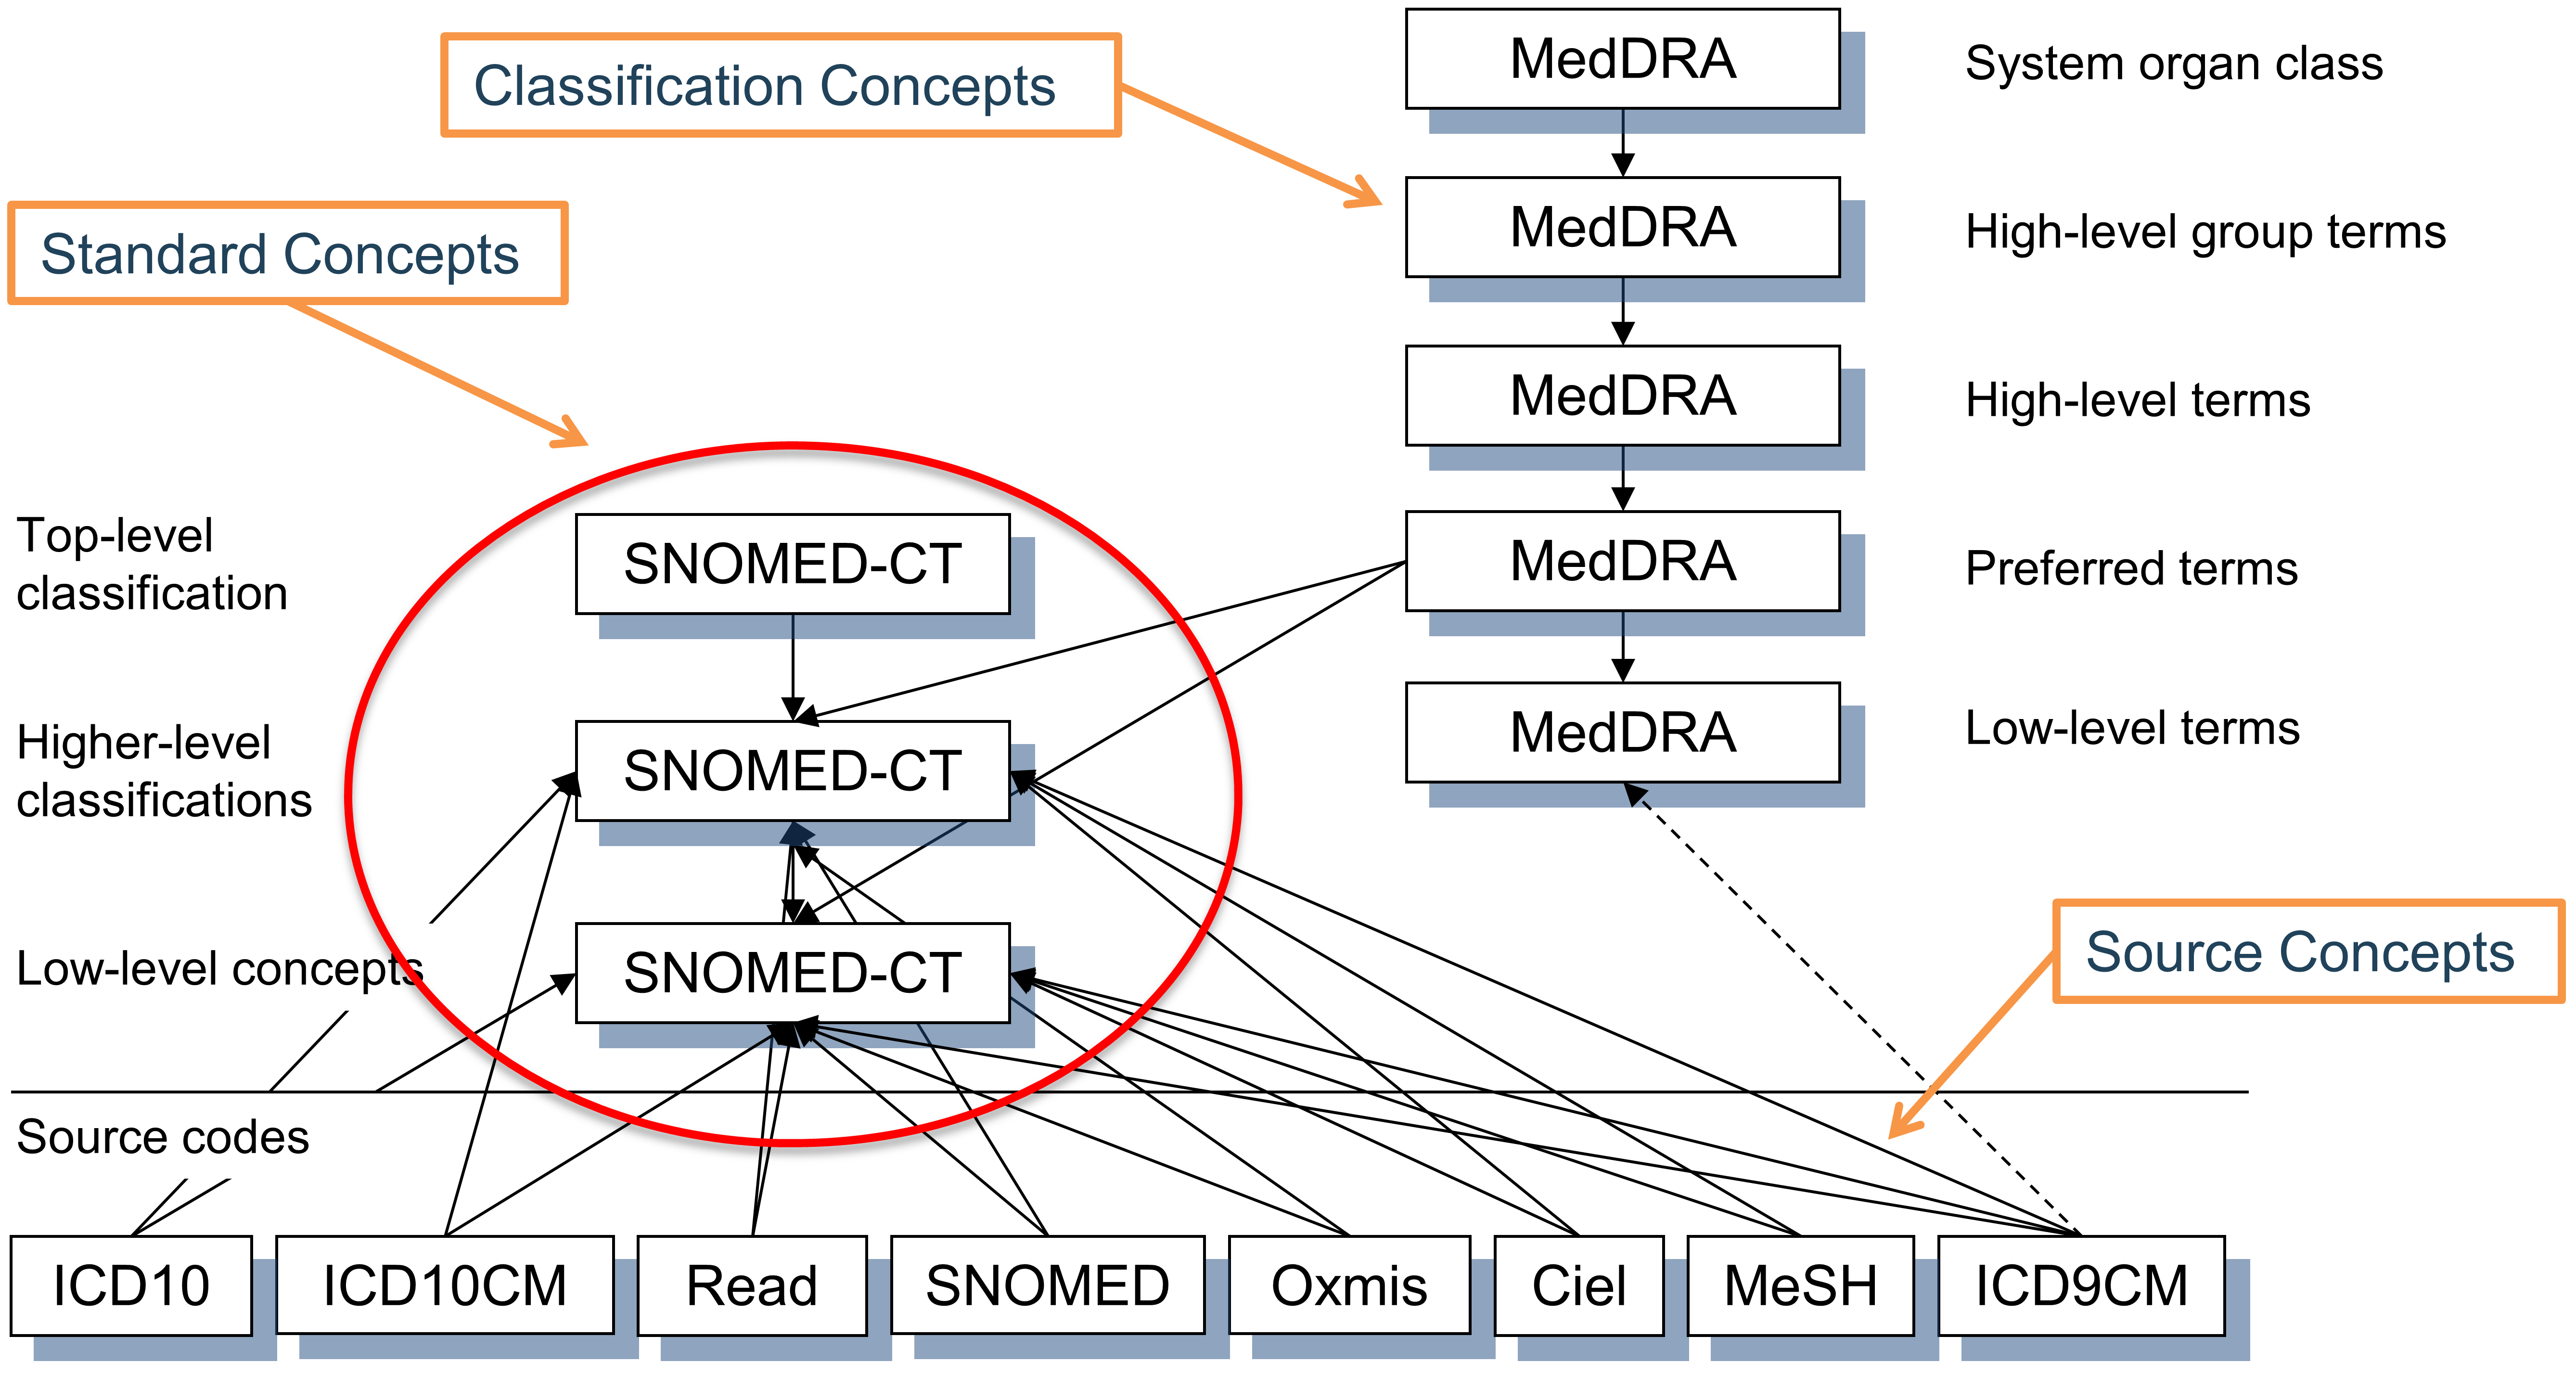
\includegraphics[width=1\linewidth]{images/StandardizedVocabularies/hierarchy} 

}

\caption{条件ドメインにおける標準、非標準ソースおよび分類コンセプトとその階層関係。SNOMEDはほとんどの標準条件コンセプトに使用されており(いくつかの腫瘍関連コンセプトはICDO3から派生)、MedDRAコンセプトは階層分類コンセプトに使用されており、他のすべてのボキャブラリは非標準またはソースコンセプトを含み、階層には参加しません。}\label{fig:hierarchy}
\end{figure}

標準、非標準、分類のコンセプトの選択は、通常各ドメインごとにボキャブラリレベルで行われます。これはコンセプトの品質、内蔵の階層、およびボキャブラリの宣言された目的に基づいています。また、すべてのボキャブラリのコンセプトが標準コンセプトとして使用されているわけではありません。各ドメインごとに別々に指定されており、各コンセプトはアクティブである必要があります(セクション@ref(コンセプトライフサイクル)参照)し、複数のボキャブラリから同じ意味を競うコンセプトがある場合、優先順位が設定されることがあります。つまり、「標準ボキャブラリ」などというものはありません。例については表\ref{tab:vocabList}を参照してください。

表: \label{tab:vocabList} 標準/非標準/分類コンセプトの割り当てに利用するボキャブラリのリスト。

\begin{longtable}[]{@{}
  >{\raggedright\arraybackslash}p{(\columnwidth - 6\tabcolsep) * \real{0.1636}}
  >{\raggedright\arraybackslash}p{(\columnwidth - 6\tabcolsep) * \real{0.2909}}
  >{\raggedright\arraybackslash}p{(\columnwidth - 6\tabcolsep) * \real{0.2909}}
  >{\raggedright\arraybackslash}p{(\columnwidth - 6\tabcolsep) * \real{0.2545}}@{}}
\toprule\noalign{}
\begin{minipage}[b]{\linewidth}\raggedright
ドメイン
\end{minipage} & \begin{minipage}[b]{\linewidth}\raggedright
標準コンセプトのためのボキャブラリ
\end{minipage} & \begin{minipage}[b]{\linewidth}\raggedright
ソースコンセプトのためのボキャブラリ
\end{minipage} & \begin{minipage}[b]{\linewidth}\raggedright
分類コンセプトのためのボキャブラリ
\end{minipage} \\
\midrule\noalign{}
\endhead
\bottomrule\noalign{}
\endlastfoot
条件 & SNOMED, ICDO3 & SNOMED Veterinary & MedDRA \\
手続き & SNOMED, CPT4, HCPCS, ICD10PCS, ICD9Proc, OPCS4 & SNOMED Veterinary, HemOnc, NAACCR & 現時点ではなし \\
測定 & SNOMED, LOINC & SNOMED Veterinary, NAACCR, CPT4, HCPCS, OPCS4, PPI & 現時点ではなし \\
薬剤 & RxNorm, RxNorm Extension, CVX & HCPCS, CPT4, HemOnc, NAACCR & ATC \\
装置 & SNOMED & 他のボキャブラリ、現在は標準化されていない & 現時点ではなし \\
観察 & SNOMED & 他のボキャブラリ & 現時点ではなし \\
訪問 & CMS Place of Service, ABMT, NUCC & SNOMED, HCPCS, CPT4, UB04 & 現時点ではなし \\
\end{longtable}

\subsection{コンセプトコード}\label{ux30b3ux30f3ux30bbux30d7ux30c8ux30b3ux30fcux30c9}

コンセプトコードはソースボキャブラリで使用される識別子です。たとえば、ICD9CMまたはNDCコードはこのフィールドに保存され、OMOPテーブルはCONCEPTテーブルへの外部キーとしてコンセプトIDを使用します。その理由は、名前空間がボキャブラリを超えて重複するためです。つまり、同じコードが異なるボキャブラリで完全に異なる意味を持つことができます(表\ref{tab:code1001}参照)。\index{concept!code}

表: \label{tab:code1001} 同じコンセプトコード1001を持つが、異なるボキャブラリ、ドメイン、コンセプトクラスのコンセプト。

\begin{longtable}[]{@{}
  >{\raggedright\arraybackslash}p{(\columnwidth - 10\tabcolsep) * \real{0.1639}}
  >{\raggedright\arraybackslash}p{(\columnwidth - 10\tabcolsep) * \real{0.0820}}
  >{\raggedright\arraybackslash}p{(\columnwidth - 10\tabcolsep) * \real{0.2131}}
  >{\raggedright\arraybackslash}p{(\columnwidth - 10\tabcolsep) * \real{0.1803}}
  >{\raggedright\arraybackslash}p{(\columnwidth - 10\tabcolsep) * \real{0.1803}}
  >{\raggedright\arraybackslash}p{(\columnwidth - 10\tabcolsep) * \real{0.1803}}@{}}
\toprule\noalign{}
\begin{minipage}[b]{\linewidth}\raggedright
コンセプトID
\end{minipage} & \begin{minipage}[b]{\linewidth}\raggedright
コンセプトコード
\end{minipage} & \begin{minipage}[b]{\linewidth}\raggedright
コンセプト名
\end{minipage} & \begin{minipage}[b]{\linewidth}\raggedright
ドメインID
\end{minipage} & \begin{minipage}[b]{\linewidth}\raggedright
ボキャブラリID
\end{minipage} & \begin{minipage}[b]{\linewidth}\raggedright
コンセプトクラス
\end{minipage} \\
\midrule\noalign{}
\endhead
\bottomrule\noalign{}
\endlastfoot
35803438 & 1001 & 顆粒球コロニー刺激因子 & 薬剤 & HemOnc & コンポーネントクラス \\
35942070 & 1001 & AJCC TNM Clin T & 測定 & NAACCR & NAACCR変数 \\
1036059 & 1001 & アンチピリン & 薬剤 & RxNorm & 成分 \\
38003544 & 1001 & レジデンシャル治療 - 精神科 & 収益コード & 収益コード & 収益コード \\
43228317 & 1001 & アセプロメタジンマレイン酸塩 & 薬剤 & BDPM & 成分 \\
45417187 & 1001 & ブロムフェニラミンマレイン酸塩、10 mg/ml注射用溶液 & 薬剤 & Multum & Multum \\
45912144 & 1001 & 血清 & 標本 & CIEL & 標本 \\
\end{longtable}

\subsection{ライフサイクル}\label{conceptLifeCycle}

ボキャブラリはめったに固定されたコード集合を持つ永久的なコーパスではありません。代わりに、コードとコンセプトは追加されたり廃止されたりします。OMOP CDMは縦断的な患者データをサポートするモデルであるため、過去に使用されたが現在はアクティブでないコンセプトや、新しいコンセプトをサポートし、それらを文脈に配置する必要があります。CONCEPTテーブルには、可能なライフサイクルの状態を説明する3つのフィールドがあります:VALID\_START\_DATE、VALID\_END\_DATE、およびINVALID\_REASON。これらのフィールドの値はコンセプトのライフサイクルの状態によって異なります:
- \textbf{アクティブまたは新しいコンセプト}
- 説明: 使用中のコンセプト。
- VALID\_START\_DATE: コンセプトの生成日、またはそれが不明な場合はボキャブラリへの取り込み日、またはそれが不明な場合は1970-1-1。
- VALID\_END\_DATE: 現在アクティブなコンセプトとして「不定期な将来で無効になる可能性があるが、現在はアクティブ」と示すための慣習として2099-12-31と設定されています。
- INVALID\_REASON: NULL
- \textbf{後継者のない廃止されたコンセプト}
- 説明: 標準コンセプトとして使用できない非アクティブなコンセプト(セクション\ref{standardConcepts}参照)。
- VALID\_START\_DATE: コンセプトの生成日、またはそれが不明な場合はボキャブラリへの取り込み日、またはそれが不明な場合は1970-1-1。
- VALID\_END\_DATE: 過去の日付で無効化を示す、またはそれが不明な場合はボキャブラリ更新の日。
- INVALID\_REASON: ``D''
- \textbf{後継者のあるアップグレードされたコンセプト}
- 説明: 非アクティブなコンセプトですが、定義された後継者があります。これらは通常、重複排除を経たコンセプトです。
- VALID\_START\_DATE: コンセプトの生成日、またはそれが不明な場合はボキャブラリ取り込み日、または1970-1-1。
- VALID\_END\_DATE: 過去の日付でアップグレードを示す、またはボキャブラリ更新の日。
- INVALID\_REASON: ``U''
- \textbf{新しいコンセプトのために再利用されたコード}
- 説明: ボキャブラリがこの廃止されたコンセプトのコードを新しいコンセプトのために再利用しました。
- VALID\_START\_DATE: コンセプトの生成日、またはそれが不明な場合は語

\section{関係}\label{ux95a2ux4fc2}

任意の2つのコンセプトは、そのドメインやボキャブラリーが同じであるかどうかに関係なく、定義された関係を持つことができます。関係の性質は、CONCEPT\_RELATIONSHIPテーブルのRELATIONSHIP\_IDフィールドにある、大文字小文字を区別する一意の英数字IDで示されます。関係は対称的であり、各関係には同等の関係が存在し、フィールドCONCEPT\_ID\_1とCONCEPT\_ID\_2の内容が入れ替わり、RELATIONSHIP\_IDはその逆に変更されます。たとえば、「Maps to」関係には反対の関係「Mapped from」があります。\index{concept!relationship}

CONCEPT\_RELATIONSHIPテーブルのレコードには、ライフサイクルフィールドRELATIONSHIP\_START\_DATE、RELATIONSHIP\_END\_DATE、およびINVALID\_REASONも含まれています。ただし、ATHENAを通じて利用可能なのはINVALID\_REASONがNULLのアクティブなレコードのみです。非アクティブな関係は内部処理のためにPallasシステムに保存されます。RELATIONSHIPテーブルは、全ての関係IDおよびその逆関係のリストを参照するためのものです。

\subsection{マッピング関係}\label{conceptMapping}

これらの関係は、非標準のコンセプトから標準コンセプトへの変換を提供し、2つの関係IDペアによってサポートされています(表\ref{tab:mappingRelationships}を参照)。\index{concept!mapping}

\begin{longtable}[]{@{}
  >{\raggedright\arraybackslash}p{(\columnwidth - 2\tabcolsep) * \real{0.2090}}
  >{\raggedright\arraybackslash}p{(\columnwidth - 2\tabcolsep) * \real{0.7910}}@{}}
\caption{\label{tab:mappingRelationships} マッピング関係の種類。}\tabularnewline
\toprule\noalign{}
\begin{minipage}[b]{\linewidth}\raggedright
関係IDペア
\end{minipage} & \begin{minipage}[b]{\linewidth}\raggedright
目的
\end{minipage} \\
\midrule\noalign{}
\endfirsthead
\toprule\noalign{}
\begin{minipage}[b]{\linewidth}\raggedright
関係IDペア
\end{minipage} & \begin{minipage}[b]{\linewidth}\raggedright
目的
\end{minipage} \\
\midrule\noalign{}
\endhead
\bottomrule\noalign{}
\endlastfoot
``Maps to''および''Mapped from'' & 標準コンセプトへのマッピング。標準コンセプトはそれ自身にマッピングされ、非標準コンセプトは標準コンセプトにマッピングされます。ほとんどの非標準コンセプトとすべての標準コンセプトは、この関係を持ち、前者は*\_SOURCE\_CONCEPT\_IDに、後者は*\_CONCEPT\_IDフィールドに保存されます。分類コンセプトはマッピングされません。 \\
``Maps to value''および''Value mapped from'' & MEASUREMENTおよびOBSERVATIONテーブルのVALUE\_AS\_CONCEPT\_IDフィールドに配置する値を表すコンセプトへのマッピング。 \\
\end{longtable}

これらのマッピング関係の目的は、同等のコンセプト間のクロスウォークを可能にし、臨床イベントがOMOP CDMでどのように表現されるかを統一することです。これは標準化されたボキャブラリの主要な成果です。

「同等のコンセプト」とは、同じ意味を持ち、さらに重要なことに、階層的に下位に含まれるコンセプトが同じ意味領域をカバーすることを意味します。同等のコンセプトが利用できず、コンセプトが標準でない場合、それはより広いコンセプト(いわゆる「上り坂マッピング」)にマッピングされます。たとえば、ICD10CM W61.51「ガチョウに噛まれる」は、標準の状態コンセプトに一般的に使用されるSNOMEDのボキャブラリには同等のものがありません。代わりに、それはSNOMED 217716004「鳥に突かれる」にマッピングされ、コンテキストとしての鳥がガチョウであるという情報が失われます。上り坂マッピングは、情報の損失が標準の研究使用ケースにとって無関係であると考えられる場合にのみ使用されます。

いくつかのマッピングは、ソースコンセプトを複数の標準コンセプトに接続します。たとえば、ICD9CM 070.43「肝性昏睡を伴うE型肝炎」は、SNOMED 235867002「急性E型肝炎」とSNOMED 72836002「肝性昏睡」の両方にマッピングされます。これは、元のソースコンセプトが肝炎と昏睡という2つの状態のあらかじめ組み合わせられたものであるためです。SNOMEDにはその組み合わせがなく、その結果、ICD9CMレコードではマッピングされた標準コンセプトそれぞれに対して2つのレコードが書かれます。

「Maps to value」関係の目的は、エンティティ-属性-値(EAV)モデルに従ったOMOP CDMテーブルの値を分割することです。これは次の状況で典型的です:

\begin{itemize}
\tightlist
\item
  検査値と結果値からなる測定値
\item
  個人または家族の疾患歴
\item
  物質に対するアレルギー
\item
  予防接種の必要性
\end{itemize}

これらの状況では、ソースコンセプトは属性(テストまたは履歴)と値(テスト結果または病気)の組み合わせです。「Maps to」関係はこのソースを属性コンセプトにマッピングし、「Maps to value」は値コンセプトにマッピングします。例については図\ref{fig:conceptValue}を参照してください。

\begin{figure}

{\centering 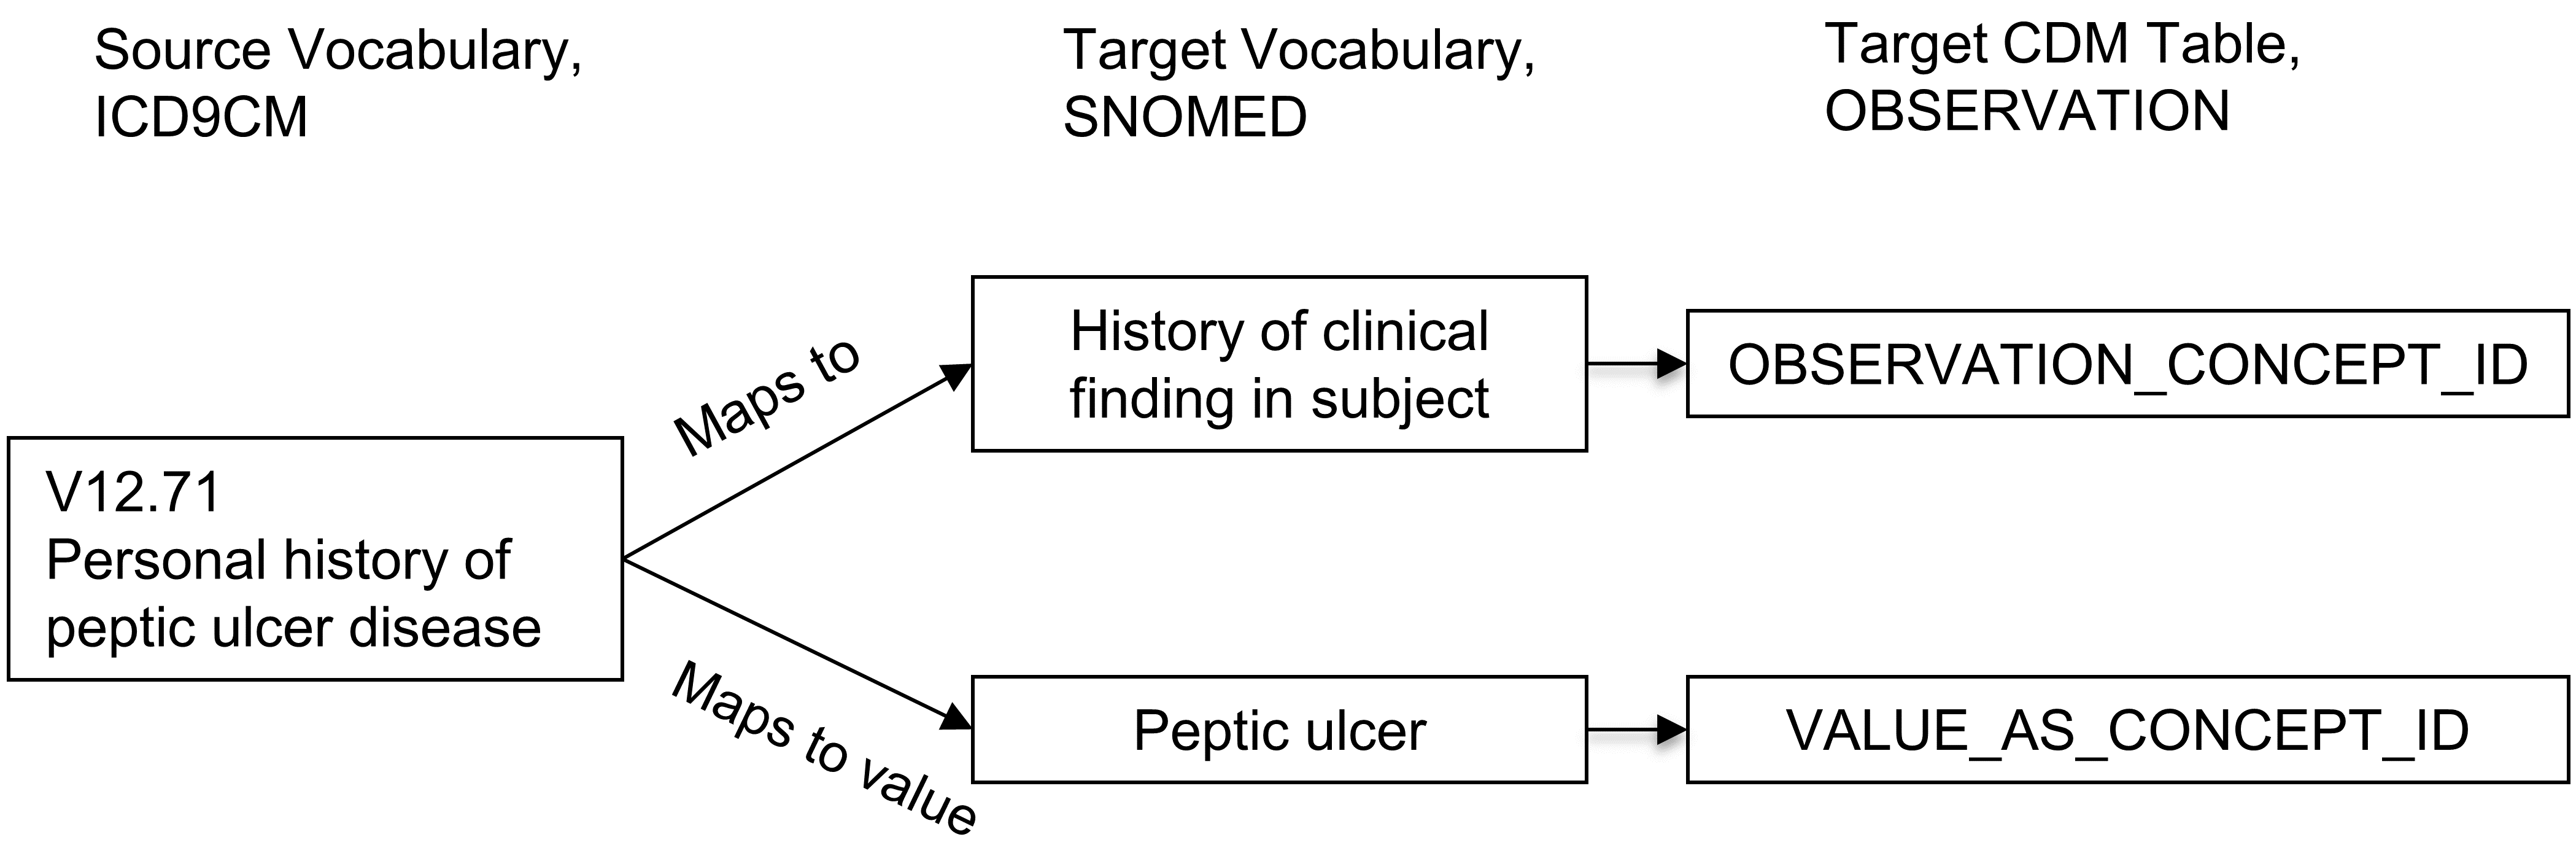
\includegraphics[width=1\linewidth]{images/StandardizedVocabularies/conceptValue} 

}

\caption{ソースコンセプトと標準コンセプトの間の一対多のマッピング。事前に組み合わせられたコンセプトは2つのコンセプトに分割され、一つは属性(ここでは臨床所見の歴史)で、もう一つは値(胃潰瘍)です。「Maps to」関係は測定または観察のドメインのコンセプトにマッピングされますが、「Maps to value」コンセプトにはドメインの制限はありません。}\label{fig:conceptValue}
\end{figure}

コンセプトのマッピングは、ネットワーク研究を行っているコミュニティの努力を支えるために提供されているOMOP標準化されたボキャブラリのもう一つの中心的な機能です。マッピング関係は外部ソースから派生するか、ボキャブラリチームによって手動で維持されます。これはそれらが完璧でないことを意味します。誤ったまたは異議のあるマッピング関係を見つけた場合、それを報告し、\href{https://forums.ohdsi.org}{フォーラム}や\href{https://github.com/OHDSI/CommonDataModel/issues}{CDMの問題}の投稿を通じてプロセスの改善に協力することが重要です。

マッピング規則の詳細な説明は、OHDSI Wikiで見つけることができます。\footnote{\url{https://www.ohdsi.org/web/wiki/doku.php?id=documentation:vocabulary:mapping}}

\subsection{階層関係}\label{ux968eux5c64ux95a2ux4fc2}

階層を示す関係は、「Is a」-「Subsumes」関係ペアによって定義されます。階層関係は、子コンセプトが親コンセプトのすべての属性に加えて1つ以上の追加属性またはより正確に定義された属性を持つように定義されます。たとえば、SNOMED 49436004「心房細動」は、SNOMED 17366009「心房性不整脈」と「Is a」関係で関連しています。両コンセプトは、不整脈のタイプが一方は細動として定義されている以外は、同一の属性セットを持っています。コンセプトは複数の親または複数の子コンセプトを持つことができます。この例では、SNOMED 49436004「心房細動」はSNOMED 40593004「細動」に対しても「Is a」に該当します。\index{concept!hierarchy}

\subsection{異なるボキャブラリーのコンセプト間の関係}\label{ux7570ux306aux308bux30dcux30adux30e3ux30d6ux30e9ux30eaux30fcux306eux30b3ux30f3ux30bbux30d7ux30c8ux9593ux306eux95a2ux4fc2}

これらの関係は通常、「Vocabulary A - Vocabulary B equivalent」のタイプであり、ボキャブラリの元のソースから提供されるか、OHDSIボキャブラリチームによって作成されます。それらは近似的なマッピングとして機能することが多いですが、より優れたマッピング関係と比較してそれほど正確ではない場合があります。高品質の同等関係(例えば、「Source - RxNorm equivalent」)は常に「Maps to」関係によって複製されます。

\subsection{同一ボキャブラリーのコンセプト間の関係}\label{ux540cux4e00ux30dcux30adux30e3ux30d6ux30e9ux30eaux30fcux306eux30b3ux30f3ux30bbux30d7ux30c8ux9593ux306eux95a2ux4fc2}

内部ボキャブラリ関係は通常、ボキャブラリプロバイダーによって提供されます。完全な説明は、OHDSI Wikiの個々のボキャブラリのボキャブラリー文書にあります。\footnote{\url{https://www.ohdsi.org/web/wiki/doku.php?id=documentation:vocabulary}}

これらの多くは、臨床イベント間の関係を定義しており、情報検索に使用することができます。例えば、尿道の障害は、「Finding site of」関係に従って見つけることができます(表\ref{tab:findingSite}を参照)。

\begin{longtable}[]{@{}ll@{}}
\caption{\label{tab:findingSite} 尿道の「Finding site of」関係で、すべてこの解剖学的構造に位置する状態を示しています。}\tabularnewline
\toprule\noalign{}
CONCEPT\_ID\_1 & CONCEPT\_ID\_2 \\
\midrule\noalign{}
\endfirsthead
\toprule\noalign{}
CONCEPT\_ID\_1 & CONCEPT\_ID\_2 \\
\midrule\noalign{}
\endhead
\bottomrule\noalign{}
\endlastfoot
4000504 ``Urethra part'' & 36713433 ``部分的尿道重複'' \\
4000504 ``Urethra part'' & 433583 ``下部尿道裂孔'' \\
4000504 ``Urethra part'' & 443533 ``男性下部尿道裂孔'' \\
4000504 ``Urethra part'' & 4005956 ``女性下部尿道裂孔'' \\
\end{longtable}

これらの関係の品質と包括性は、元のボキャブラリーの品質によって異なります。一般に、標準コンセプトを抽出するために使用されるボキャブラリーは、より良いキュレーションのために選ばれ、そのため、内部関係の品質も高い傾向があります。

\section{階層}\label{conceptAncestor}

ドメイン内では、標準および分類コンセプトは階層構造に組織され、CONCEPT\_ANCESTORテーブルに格納されています。これにより、コンセプトとその下位層に含まれる属性をすべてクエリして取得することが可能です。これらの下位層に含まれる属性は祖先と同じ属性を持ちますが、追加の属性や、より定義された属性も持ちます。

CONCEPT\_ANCESTORテーブルは、CONCEPT\_RELATIONSHIPテーブルからすべての可能なコンセプトを階層関係を通じて走査して自動的に構築されます。これらは ``Is a'' - ``Subsumes'' のペア(図 \ref{fig:conceptAncestor} 参照)や、ボキャブラリ間の階層を接続する他の関係です。どの関係が階層構造に参加するかは、RELATIONSHIP参照テーブルのDEFINES\_ANCESTRYフラグにより各関係IDに対して定義されます。



\begin{figure}

{\centering 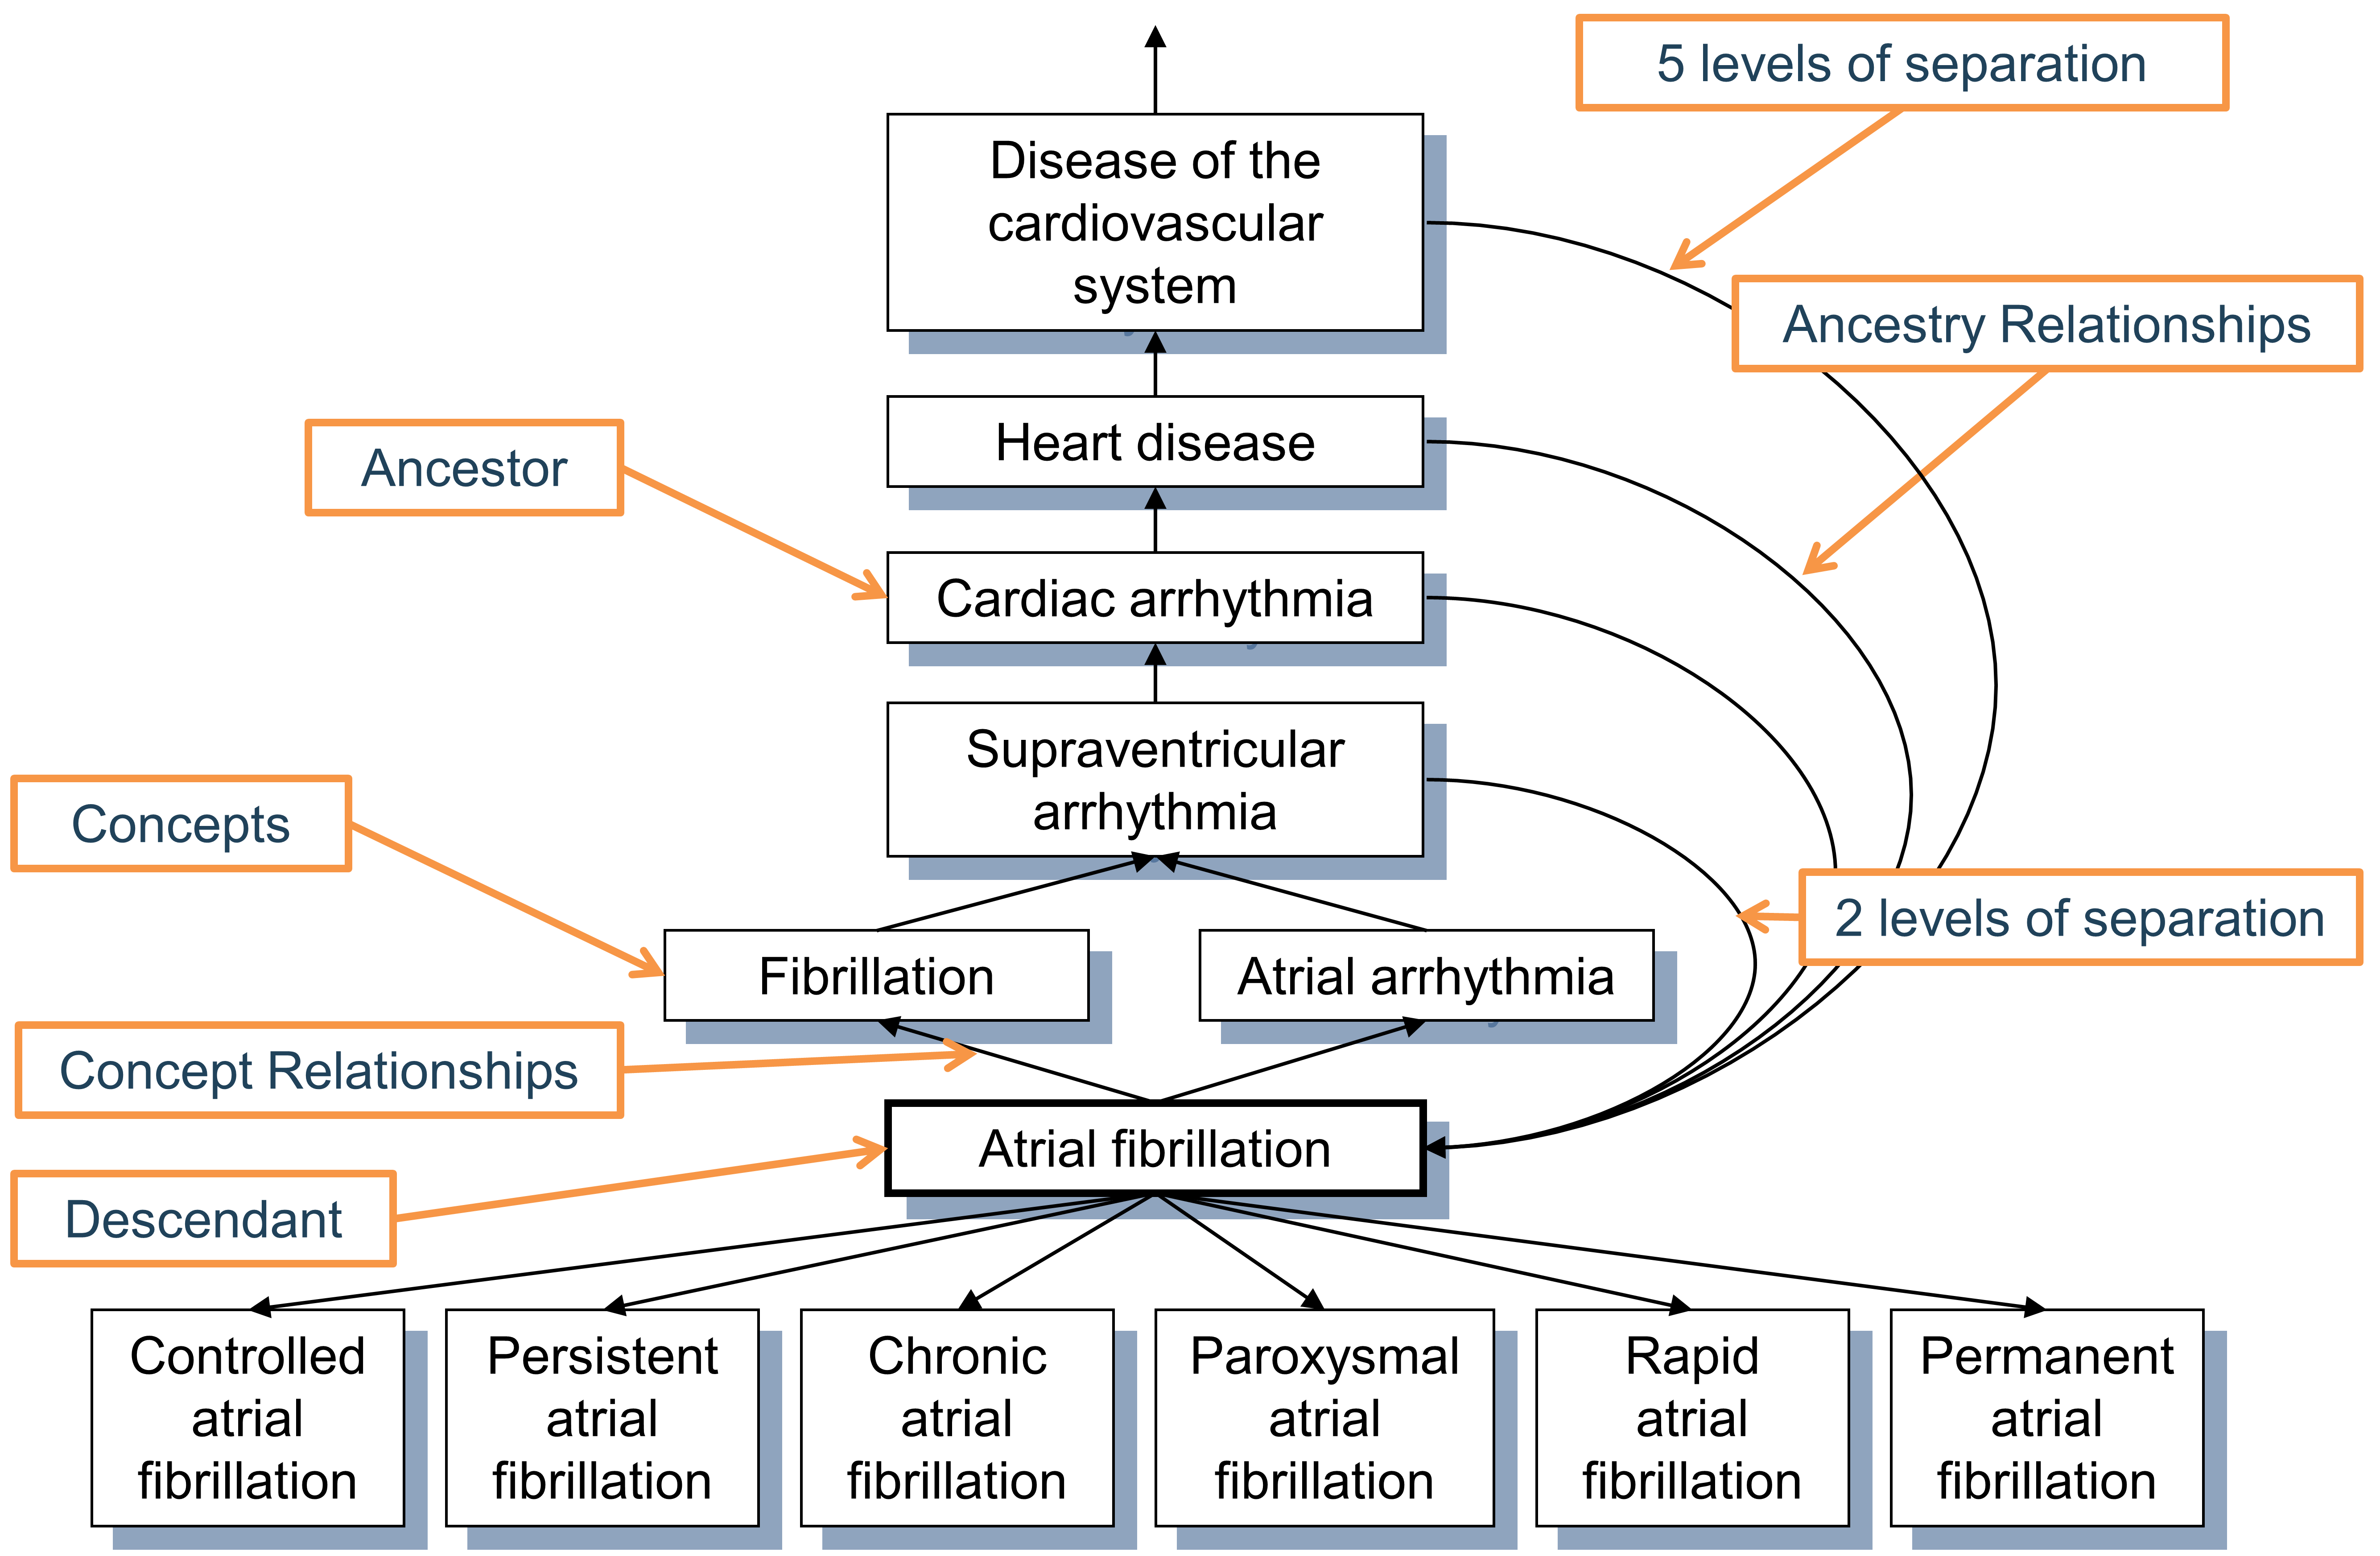
\includegraphics[width=1\linewidth]{images/StandardizedVocabularies/conceptAncestor} 

}

\caption{「心房細動」の階層。第一度の系譜は「Is a」と「Subsumes」関係によって定義され、高次の関係は推論され、CONCEPT\_ANCESTORテーブルに保存されます。各コンセプトは、そのレベルの分離が0とされるでも自身の下位層でもあります。 \index{コンセプト!祖先}}\label{fig:conceptAncestor}
\end{figure}

祖先の度合い、つまり祖先と子孫の間のステップ数は、MIN\_LEVELS\_OF\_SEPARATIONおよびMAX\_LEVELS\_OF\_SEPARATIONフィールドに記録され、最短または最長の接続を定義します。すべての階層的な関係が分離度の計算に等しく寄与するわけではありません。この度合いにカウントされるステップは、各関係IDに対してRELATIONSHIP参照テーブルのIS\_HIERARCHICALフラグによって決まります。

現在のところ、完全で高品質な階層は薬剤とコンディションの2つのドメインにのみ存在します。処置、測定値、および観察のドメインは部分的にしかカバーされておらず、まだ構築途中です。特に薬剤のドメインでは、成分や薬剤クラスのメンバーを原産地、ブランド名、その他の属性に関係なく参照できるため、祖先関係は非常に有用です。

\section{内部参照テーブル}\label{ux5185ux90e8ux53c2ux7167ux30c6ux30fcux30d6ux30eb}

DOMAIN\_ID、VOCABULARY\_ID、CONCEPT\_CLASS\_ID(すべてCONCEPTレコード内)およびCONCEPT\_RELATIONSHIP\_ID(CONCEPT\_RELATIONSHIP内)はそれぞれ独自のボキャブラリによって制御されます。これらは、主キーとしての*\_IDフィールド、詳細な*\_NAMEフィールド、およびCONCEPTテーブルに戻る参照を持つ*\_CONCEPT\_IDフィールドを持つ4つの参照テーブルDOMAIN、VOCABULARY、CONCEPT\_CLASS、およびRELATIONSHIPで定義されています。これらの重複レコードの目的は、自動ナビゲーションエンジンをサポートする情報モデルを提供することです。

VOCABULARYテーブルには、元のボキャブラリのソースとバージョンを参照するためのVOCABULARY\_REFERENCEおよびVOCABULARY\_VERSIONフィールドも含まれています。RELATIONSHIPテーブルには、DEFINES\_ANCESTRY、IS\_HIERARCHICAL、およびREVERSE\_RELATIONSHIP\_IDフィールドが追加されています。後者は、関係のペアに対するカウンター関係IDを定義します。

\section{特別な状況}\label{specialSituations}

\subsection{性別}\label{ux6027ux5225}

OMOP CDMと標準化されたボキャブラリにおける性別は、出生時の生物学的性別を表します。しばしば、代替の性別を定義する方法についての質問が寄せられます。これらのユースケースは、OBSERVATIONテーブルに記録された人物の自己定義の性別を通じてカバーされる必要があります(そのデータ資産にそのような情報が含まれている場合)。

\subsection{人種と民族}\label{ux4ebaux7a2eux3068ux6c11ux65cf}

これらは米国政府の定義に従います。民族はヒスパニック系または非ヒスパニック系の区別であり、どのレースでもあり得ます。人種は一般的に5つの主要な人種に分けられ、これらは階層的な子孫として民族を持ちます。混合人種は含まれていません。

\subsection{診断コーディングシステムとOMOPのコンディション}\label{ux8a3aux65adux30b3ux30fcux30c7ux30a3ux30f3ux30b0ux30b7ux30b9ux30c6ux30e0ux3068omopux306eux30b3ux30f3ux30c7ux30a3ux30b7ux30e7ux30f3}

一般的に使用されるコーディングシステム(例:ICD-9やICD-10)は、適切な診断処理に基づいて診断をより明確に定義します。コンディションドメインはこの意味構造と完全に一致するわけではなく、一部重なります。例えば、コンディションには診断が導かれる前の兆候や症状も含まれ、ICDコードには他のドメインに属するコンセプトも含まれます(例:処置)。

\subsection{処置コードシステム}\label{ux51e6ux7f6eux30b3ux30fcux30c9ux30b7ux30b9ux30c6ux30e0}

同様に、HCPCSやCPT4のようなコーディングシステムは医療手技のリストと考えられます。しかし実際には、これらは医療サービスの支払いのための正当化としてのメニューのようなものです。これらのサービスの多くは処置ドメインに含まれますが、多くのコンセプトはこの範囲外です。

\subsection{デバイス}\label{ux30c7ux30d0ux30a4ux30b9}

デバイスのコンセプトについては、標準コンセプトのソースとして使用できる標準化されたコーディングスキームがありません。多くのソースデータでは、デバイスはコード化されていないか、外部のコーディングスキームに含まれていません。同じ理由で、現在利用可能な階層システムはありません。

\subsection{受診期間とサービス}\label{ux53d7ux8a3aux671fux9593ux3068ux30b5ux30fcux30d3ux30b9}

受診期間のコンセプトは、医療受診の性質を定義します。多くのソースシステムでは、これらはサービスの場所として呼ばれており、病院などの組織や物理的構造を示します。その他では、サービスと呼ばれます。これらは国ごとに異なり、その定義を得るのは困難です。医療施設はしばしば特定の受診期間(例えばXYZ病院)に特化していますが、それによって定義されるべきではありません(XYZ病院でも患者が病院以外の受診に遭遇する可能性があります)。

\subsection{プロバイダーと専門分野}\label{ux30d7ux30edux30d0ux30a4ux30c0ux30fcux3068ux5c02ux9580ux5206ux91ce}

どの人間の医療提供者も医療提供者ドメインに定義されています。これには、医師や看護師のような医療専門職だけでなく、眼鏡技師や靴職人のような非医療提供者も含まれます。専門分野は、プロバイダー「医師」の下位層に含まれます。医療施設は専門分野を持つことはできませんが、主要スタッフの専門分野によって定義されることがよくあります(「外科部門」など)。

\subsection{特別な要件を持つ治療領域}\label{ux7279ux5225ux306aux8981ux4ef6ux3092ux6301ux3064ux6cbbux7642ux9818ux57df}

標準化されたボキャブラリは包括的にヘルスケアのすべての側面をカバーしています。しかし、いくつかの治療領域には特別なニーズがあり、特別なボキャブラリが必要です。例としては、腫瘍学、放射線学、ゲノミクスが挙げられます。これらの拡張を開発するために、特別なOHDSIワーキンググループが存在します。その結果、OMOPで標準化されたボキャブラリは、異なる起源と目的を持つコンセプトがすべて同じドメイン固有の階層に存在する統合システムを構成しています。

\subsection{薬剤ドメインにおける標準コンセプト}\label{rxNormExtension}

薬剤ドメインの多くのコンセプトは、米国国立医学図書館が生産する公的に利用可能なボキャブラリであるRxNormから供給されます。しかし、米国外の薬剤は、成分、形態、および強度の組み合わせが米国で市販されているかどうかに応じてカバーされない場合があります。米国市場にない薬剤は、OHDSIボキャブラリチームによって、唯一の大規模ドメインボキャブラリである\href{https://www.ohdsi.org/web/wiki/doku.php?id=documentation:vocabulary:rxnorm_extension}{RxNorm Extension}というボキャブラリのもとに追加されます。

\subsection{NULLのフレーバー}\label{nullux306eux30d5ux30ecux30fcux30d0ux30fc}

多くのボキャブラリには情報の欠如に関するコードが含まれています。例えば、5つの性別コンセプト8507「男性」、8532「女性」、8570「曖昧」、8551「不明」、および8521「その他」のうち、標準コンセプトは最初の2つのみであり、他の3つはマッピングなしのソースコンセプトです。標準化されたボキャブラリでは、なぜ情報が利用できないかの区別はありません。それは患者による情報の積極的な撤回、欠落値、何らかの形で定義または標準化されていない値、またはCONCEPT\_RELATIONSHIPでのマッピング記録の欠如によるものである可能性があります。このようなコンセプトはマッピングされず、標準コンセプトのコンセプトID=0のデフォルトマッピングに対応します。

\section{まとめ}\label{ux307eux3068ux3081-3}

\begin{rmdsummary}
\begin{itemize}
\tightlist
\item
  すべてのイベントと管理的事実は、OMOP標準ボキャブラリでコンセプト、コンセプト関係、およびコンセプト祖先階層として表されます。
\item
  これらのほとんどは既存のコーディングスキームやボキャブラリから採用されますが、一部はOHDSIボキャブラリチームによって新たにキュレーションされます。
\item
  すべてのコンセプトにはドメインが割り当てられ、そのコンセプトが表す事実がCDMに格納される場所を制御します。
\item
  異なるボキャブラリの同等の意味のコンセプトは、そのうちの1つにマppingされ、これが標準コンセプトとして指定されます。他のものはソースコンセプトです。
\item
  マッピングは「Maps to」および「Maps to value」というコンセプト関係を通じて行われます。
\item
  分類コンセプトという追加のコンセプトクラスがあり、これらは非標準ですが、ソースコンセプトとは異なり、階層に参加します。
\item
  コンセプトは時間とともにライフサイクルを持ちます。
\item
  ドメイン内のコンセプトは階層に整理されています。階層の質はドメインごとに異なり、階層システムの完成は進行中の作業です。
\item
  間違いや不正確さを発見した場合は、コミュニティに積極的に参加することを強くお勧めします。
\end{itemize}
\end{rmdsummary}

\section{演習}\label{ux6f14ux7fd2}

\subsubsection*{前提条件}\label{ux524dux63d0ux6761ux4ef6-2}
\addcontentsline{toc}{subsubsection}{前提条件}

最初の演習では、標準ボキャブラリのコンセプトを調べる必要があります。これはATHENA\footnote{\url{http://athena.ohdsi.org/}}またはATLAS\footnote{\url{http://atlas-demo.ohdsi.org}}を通じて行うことができます。

\begin{exercise}
\protect\hypertarget{exr:exerciseVocab1}{}\label{exr:exerciseVocab1}``胃腸出血''の標準コンセプトIDは何ですか?
\end{exercise}

\begin{exercise}
\protect\hypertarget{exr:exerciseVocab2}{}\label{exr:exerciseVocab2}``胃腸出血''の標準コンセプトにマッピングされるICD-10CMコードはどれですか?この標準コンセプトにマッピングされるICD-9CMコードはどれですか?
\end{exercise}

\begin{exercise}
\protect\hypertarget{exr:exerciseVocab3}{}\label{exr:exerciseVocab3}``胃腸出血''の標準コンセプトと同等のMedDRA推奨用語は何ですか?
\end{exercise}

提案された回答は付録 \ref{Vocabanswers}に記載されています。

\chapter{第6章 --翻訳作業中-- 抽出、変換、ロード}\label{ExtractTransformLoad}

\emph{章の著者: Clair Blacketer \& Erica Voss}

\section{はじめに}\label{ux306fux3058ux3081ux306b}

ネイティブ/生データからOMOP共通データモデル(CDM)に移行するためには、抽出、変換、ロード(ETL)プロセスを作成する必要があります。このプロセスでは、データをCDMに再構築し、標準化されたボキャブラリへのマッピングを追加します。これは通常、一連の自動化スクリプト、例えばSQLスクリプトとして実装されます。このETLプロセスは、ソースデータが更新されたときに再実行できるよう、再現可能であることが重要です。\index{ETL|see {抽出、変換、ロード(ETL)}} \index{生データ} \index{ネイティブデータ|see {生データ}} \index{ソースデータ|see {生データ}}

ETLの作成は通常、大規模な取り組みとなります。長年にわたり、私たちは以下の4つの主要なステップからなるベストプラクティスを開発しました:

\begin{enumerate}
\def\labelenumi{\arabic{enumi}.}
\tightlist
\item
  データの専門家とCDMの専門家が共同でETLをデザインする。
\item
  医学的知識を持つ人がコーディングのマッピングを作成する。
\item
  技術者がETLを実装する。
\item
  全員が品質管理に関与する。
\end{enumerate}

この章では、これらのステップそれぞれについて詳細に議論します。OHDSIコミュニティによっていくつかの支援ツールが開発されており、これらについても議論します。この章を締めくくるにあたり、CDMとETLのメンテナンスについても議論します。
\#\# ステップ 1: ETLのデザイン

ETLのデザインと実装を明確に分けることが重要です。ETLのデザインにはソースデータとCDMの両方に関する広範な知識が必要です。一方、ETLの実装は通常、ETLを計算効率的に行うための技術的専門知識に依存します。両方を同時に行おうとすると、細かい点に気を取られてしまうことが多く、全体像に集中できなくなることがあります。

ETLデザインプロセスを支援するために密接に統合された2つのツールが開発されました:White RabbitとRabbit-in-a-Hatです。

\subsection{White Rabbit}\label{white-rabbit}

データベースでETLプロセスを開始するためには、データ(テーブル、フィールド、内容)を理解する必要があります。これが\href{https://github.com/OHDSI/WhiteRabbit}{White Rabbit}の役割です。White Rabbitは、縦断的な医療データベースを\href{https://github.com/OHDSI/CommonDataModel}{OMOP CDM}にETLするための準備を支援するソフトウェアツールです。White Rabbitはデータをスキャンし、ETLのデザインを開始するために必要なすべての情報を含むレポートを作成します。全てのソースコードとインストール手順、およびマニュアルへのリンクはGitHubで入手可能です\footnote{\url{https://github.com/OHDSI/WhiteRabbit}.}。\index{White Rabbit} \index{data profiling|see {White Rabbit}}

\subsubsection*{範囲と目的}\label{ux7bc4ux56f2ux3068ux76eeux7684}
\addcontentsline{toc}{subsubsection}{範囲と目的}

White Rabbitの主な機能は、ソースデータをスキャンし、フィールドに出現するテーブル、フィールド、値に関する詳細な情報を提供することです。ソースデータは、カンマ区切りのテキストファイルやデータベース(MySQL、SQL Server、Oracle、PostgreSQL、Microsoft APS、Microsoft Access、Amazon Redshift)に保存できます。スキャンによって、ETLデザイン時に参考文献として使用できるレポートが生成されます。例えば、Rabbit-In-a-Hatツールと一緒に使用することができます。White Rabbitは標準的なデータプロファイリングツールと異なり、生成された出力データファイルに個人識別情報(PII)を表示しないようにします。

\subsubsection*{プロセス概要}\label{ux30d7ux30edux30bbux30b9ux6982ux8981}
\addcontentsline{toc}{subsubsection}{プロセス概要}

ソフトウェアを使用してソースデータをスキャンする一般的な手順:

\begin{enumerate}
\def\labelenumi{\arabic{enumi}.}
\tightlist
\item
  結果をエクスポートするローカルデスクトップコンピュータの作業フォルダを設定します。
\item
  ソースデータベースまたはCSVテキストファイルに接続し、接続をテストします。
\item
  スキャン対象のテーブルを選択し、テーブルをスキャンします。
\item
  White Rabbitがソースデータに関する情報をエクスポートします。
\end{enumerate}

\subsubsection*{作業フォルダの設定}\label{ux4f5cux696dux30d5ux30a9ux30ebux30c0ux306eux8a2dux5b9a}
\addcontentsline{toc}{subsubsection}{作業フォルダの設定}

White Rabbitアプリケーションをダウンロードしてインストールした後、最初に行うべきことは作業フォルダを設定することです。White Rabbitが作成するすべてのファイルはこのローカルフォルダにエクスポートされます。図\ref{fig:WhiteRabbitLocation}に示されている「Pick Folder」ボタンを使用して、スキャンドキュメントを配置するローカル環境をナビゲートします。

\begin{figure}

{\centering 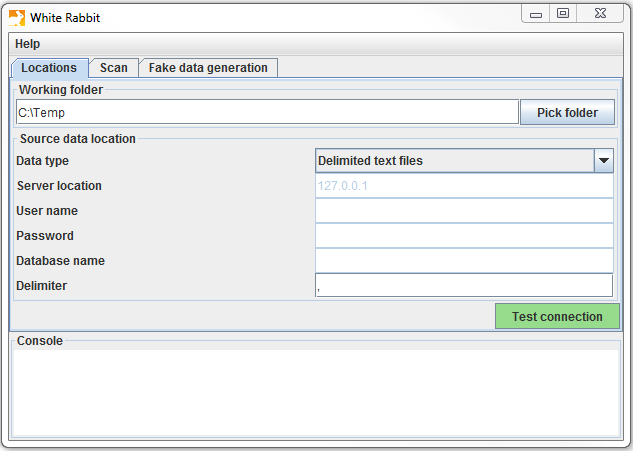
\includegraphics[width=1\linewidth]{images/ExtractTransformLoad/WhiteRabbitLocation} 

}

\caption{White Rabbitアプリケーションの作業フォルダを指定するための「Pick Folder」ボタン。}\label{fig:WhiteRabbitLocation}
\end{figure}

\subsubsection*{データベースへの接続}\label{ux30c7ux30fcux30bfux30d9ux30fcux30b9ux3078ux306eux63a5ux7d9a}
\addcontentsline{toc}{subsubsection}{データベースへの接続}

White Rabbitは区切りテキストファイルとさまざまなデータベースプラットフォームをサポートします。各フィールドにマウスカーソルを置くと、必要な情報が表示されます。詳細についてはマニュアルをご覧ください。

\subsubsection*{データベース内のテーブルをスキャン}\label{ux30c7ux30fcux30bfux30d9ux30fcux30b9ux5185ux306eux30c6ux30fcux30d6ux30ebux3092ux30b9ux30adux30e3ux30f3}
\addcontentsline{toc}{subsubsection}{データベース内のテーブルをスキャン}

データベースに接続した後、含まれるテーブルをスキャンできます。スキャンによってETLのデザインに役立つ情報を含むレポートが生成されます。図\ref{fig:WhiteRabbitAddTables}に示されたスキャンタブを使用して、「Add」(Ctrl + マウスクリック)をクリックすることで、選択されたソースデータベース内の個々のテーブルを選択するか、データベース内のすべてのテーブルを自動選択する「Add all in DB」ボタンをクリックできます。

\begin{figure}

{\centering 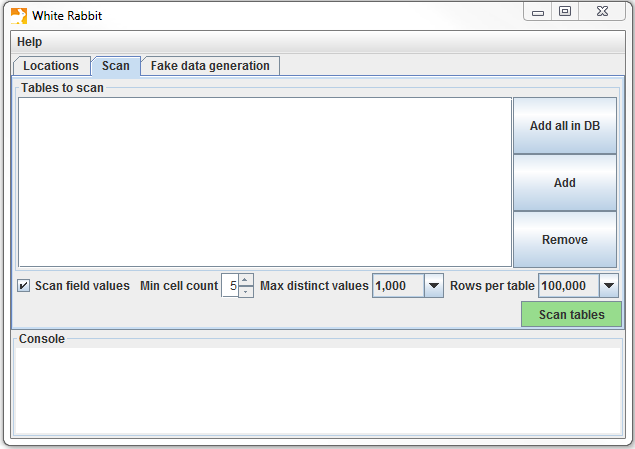
\includegraphics[width=1\linewidth]{images/ExtractTransformLoad/WhiteRabbitAddTables} 

}

\caption{White Rabbit スキャンタブ。}\label{fig:WhiteRabbitAddTables}
\end{figure}

スキャンにはいくつかの設定オプションもあります:

\begin{itemize}
\tightlist
\item
  「フィールド値をスキャン」をチェックすると、WhiteRabbitは列に表示される値を調査します。
\item
  「最小セル数」はフィールド値のスキャン時のオプションです。デフォルトでは5に設定されており、ソースデータで5回未満表示された値は報告に表示されません。個別のデータセットには、この最小セル数に関する独自のルールがある場合があります。
\item
  「テーブルあたりの行数」はフィールド値のスキャン時のオプションです。デフォルトでは、White Rabbitはテーブル内の100,000行をランダムに選択してスキャンします。
\end{itemize}

すべての設定が完了したら、「テーブルをスキャン」ボタンを押します。スキャンが完了すると、レポートが作業フォルダに書き込まれます。

\subsubsection*{スキャンレポートの解釈}\label{ux30b9ux30adux30e3ux30f3ux30ecux30ddux30fcux30c8ux306eux89e3ux91c8}
\addcontentsline{toc}{subsubsection}{スキャンレポートの解釈}

スキャンが完了すると、スキャンされた各テーブルと概要タブを含むExcelファイルが選択されたフォルダに生成されます。概要タブにはスキャンされたすべてのテーブル、各テーブルの各フィールド、各フィールドのデータ型、フィールドの最大長、テーブル行数、スキャンされた行数、および各フィールドが空である頻度が一覧表示されます。図\ref{fig:ScanOverviewTab}.に示されたサンプル概要タブ。

\begin{figure}

{\centering 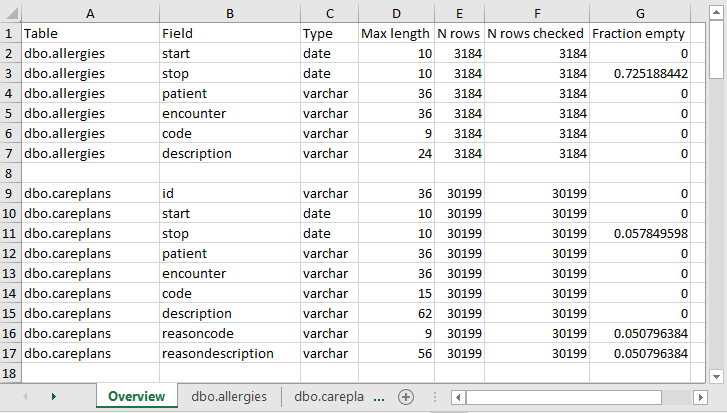
\includegraphics[width=1\linewidth]{images/ExtractTransformLoad/ScanOverviewTab} 

}

\caption{スキャンレポートのサンプル概要タブ。}\label{fig:ScanOverviewTab}
\end{figure}

各テーブルのタブには、各フィールド、各フィールド内の値、および各値の頻度が表示されます。各ソーステーブル列は、Excelに2つの列を生成します。1つの列には、スキャン時に設定された「最小セル数」を超えるすべての固有値がリストされます。固有値のリストが切り捨てられた場合、リストの最後の値は「リスト切り捨て」と表示されます。これは、「最小セル数」で入力した数より少ない頻度で表示される1つ以上の追加の固有ソース値が存在することを示します。各固有値の横には、その値がサンプルに出現する頻度(発生回数)を含む2番目の列もあります。これらの2つの列(固有値と頻度)は、ワークブック内のプロファイリングされたテーブルのすべてのソースカラムについて繰り返されます。

\begin{figure}

{\centering 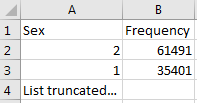
\includegraphics[width=0.3\linewidth]{images/ExtractTransformLoad/ScanSex} 

}

\caption{単一列のサンプル値。}\label{fig:scanSex}
\end{figure}

レポートはソースデータを理解するために強力であり、存在するものを強調します。例えば、図\ref{fig:scanSex}に示された結果がスキャンされたテーブルの「Sex」列に戻された場合、2つの一般的な値(1と2)がそれぞれ61,491回と35,401回出現したことが分かります。White Rabbitは1を男性、2を女性として定義することはなく、データホルダーが通常、ソースシステムに固有のソースコードを定義する必要があります。しかし、これらの2つの値(1と2)はデータに存在する唯一の値ではなく、このリストが切り捨てられたことが確認できます。これらの他の値は非常に低い頻度で出現し(「最小セル数」で定義)、しばしば不正確または非常に疑わしい値を表しています。ETLを生成する際には、高頻度のジェンダーコンセプト1と2を処理するだけでなく、この列に存在する他の低頻度の値にも対応するよう計画する必要があります。例えば、これらの低頻度のジェンダーが「NULL」であれば、そのデータを処理し、その状況に対処する方法をETLが知っていることを確認したいです。

\subsection{Rabbit-In-a-Hat}\label{rabbit-in-a-hat}

White Rabbitスキャンを手にしたら、ソースデータの全体像が掴めます。次に、これをCDMに変換するためのロジックを定義する必要があります。このデザイン作業には、ソースデータとCDMの両方に関する深い知識が必要です。White Rabbitソフトウェアと共に提供されるRabbit-in-a-Hatツールは、これらの分野の専門家チームをサポートするように特別にデザインされています。典型的な設定では、ETLデザインチームが一緒に部屋に集まり、Rabbit-in-a-Hatがスクリーンに投影されます。最初のラウンドでは、テーブル間のマッピングがコラボレーションで決定され、その後、フィールド間のマッピングがデザインされ、値をどのように変換するかのロジックが定義されます。\index{Rabbit-In-A-Hat} \index{ETL design|see {Rabbit-In-A-Hat}}

\subsubsection*{範囲と目的}\label{ux7bc4ux56f2ux3068ux76eeux7684-1}
\addcontentsline{toc}{subsubsection}{範囲と目的}

Rabbit-In-a-HatはWhite Rabbitスキャンドキュメントを読み取り、表示するようにデザインされています。White Rabbitはソースデータに関する情報を生成し、Rabbit-In-a-Hatはその情報を使用して、グラフィカルユーザーインターフェイスを通じてソースデータをCDMのテーブルおよびカラムに接続することを可能にします。Rabbit-In-a-HatはETLプロセスのドキュメントを生成しますが、ETLを作成するコードは生成しません。

\subsubsection*{プロセス概要}\label{ux30d7ux30edux30bbux30b9ux6982ux8981-1}
\addcontentsline{toc}{subsubsection}{プロセス概要}

このソフトウェアを使用してETLのドキュメントを生成する一般的な手順:

\begin{enumerate}
\def\labelenumi{\arabic{enumi}.}
\tightlist
\item
  White Rabbitのスキャン結果を完了させます。
\item
  スキャン結果を開くと、インターフェースにソーステーブルおよびCDMテーブルが表示されます。
\item
  ソーステーブルを対応するCDMテーブルに接続します。
\item
  各ソーステーブルからCDMテーブルへの接続について、ソース列からCDM列への詳細を定義します。
\item
  Rabbit-In-a-Hatの作業内容を保存し、MS Wordドキュメントにエクスポートします。
\end{enumerate}

\subsubsection*{ETLロジックの記述}\label{etlux30edux30b8ux30c3ux30afux306eux8a18ux8ff0}
\addcontentsline{toc}{subsubsection}{ETLロジックの記述}

White RabbitスキャンレポートをRabbit-In-a-Hatで開いたら、ソースデータをOMOP CDMに変換する方法のロジックをデザインし、記述する準備が整います。次のセクションでは、Synthea\footnote{Synthea\textsuperscript{TM}は実際の患者をモデル化することを目的とした患者ジェネレーターです。データはアプリケーションに渡されたパラメータに基づいて作成されます。データの構造については、\href{https://github.com/synthetichealth/synthea/wiki}{こちら}をご覧ください。}データベースのいくつかのテーブルが変換中にどのように見えるかを例示します。

\subsubsection*{ETLの一般的なフロー}\label{etlux306eux4e00ux822cux7684ux306aux30d5ux30edux30fc}
\addcontentsline{toc}{subsubsection}{ETLの一般的なフロー}

CDMは人中心のモデルであるため、まずPERSONテーブルをマッピングすることが常に良い考えです。すべての臨床イベントテーブル(CONDITION\_OCCURRENCE、DRUG\_EXPOSURE、PROCEDURE\_OCCURRENCEなど)は、person\_idを介してPERSONテーブルを参照しているため、最初にPERSONテーブルのロジックを解決すると、後で簡単になります。PERSONテーブルの後は、OBSERVATION\_PERIODテーブルを次に変換するのが良いルールです。CDMデータベースの各人物には少なくとも1つのOBSERVATION\_PERIODがあり、一般的に、人物のほとんどのイベントはこの期間内に発生します。PERSONおよびOBSERVATION\_PERIODテーブルが完了したら、次は通常、PROVIDER、CARE\_SITE、およびLOCATIONなどの次元テーブルを変換します。臨床テーブルの前に処理すべき最後のテーブルロジックはVISIT\_OCCURRENCEです。これはしばしばETL全体で最も複雑なロジックであり、最も重要なものの1つです。人物の患者の旅の過程で発生するほとんどのイベントは受診期間中に発生します。これらのテーブルが完了したら、どのCDMテーブルを変換し、その順序を選択できます。

\begin{figure}

{\centering 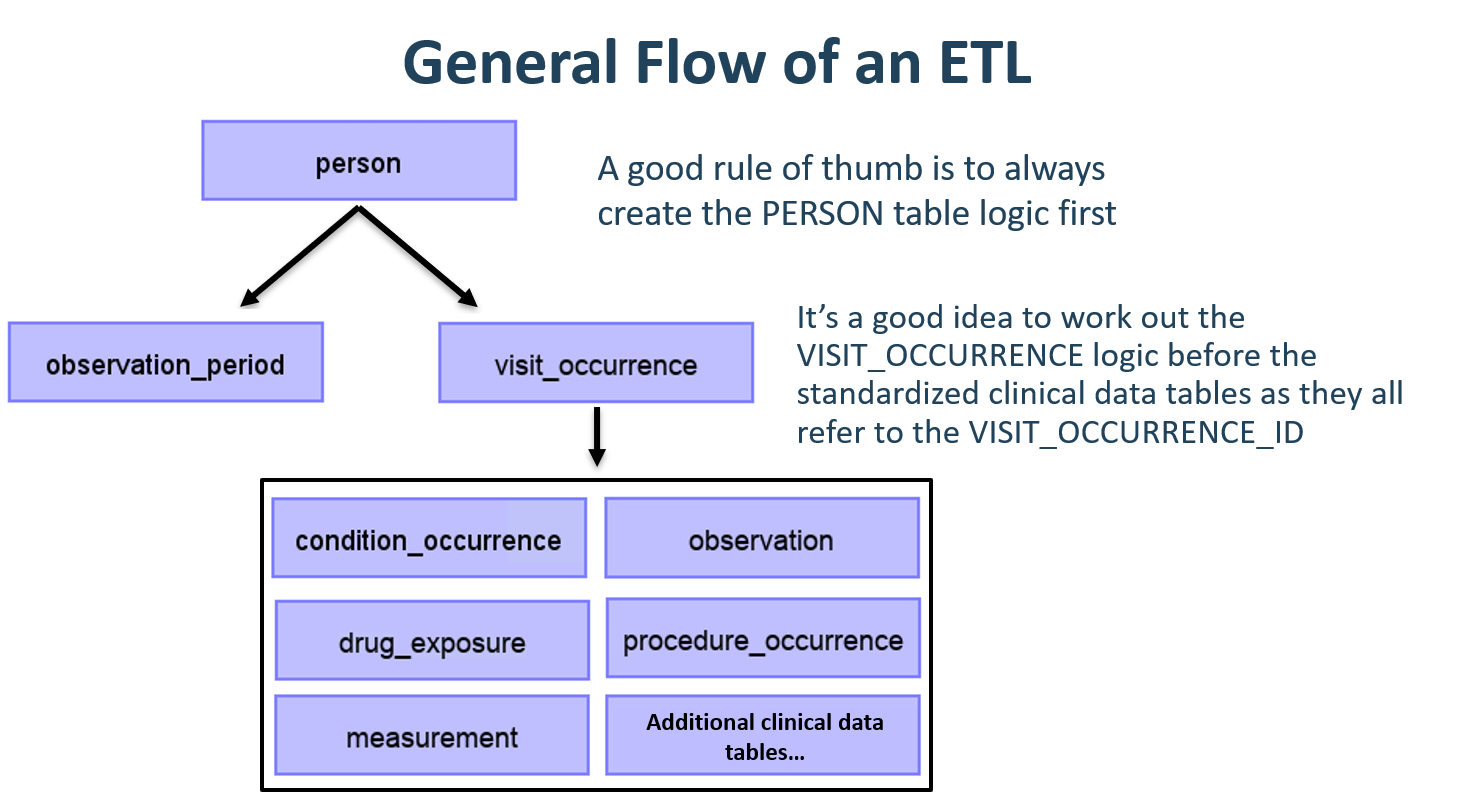
\includegraphics[width=1\linewidth]{images/ExtractTransformLoad/flowOfEtl} 

}

\caption{ETLの一般的なフローと、最初にマッピングするテーブル。}\label{fig:etlFlow}
\end{figure}

CDM変換中に中間テーブルを作成する必要があることがよくあります。これは、イベントに正しいVISIT\_OCCURRENCE\_IDを割り当てるため、またはソースコードを標準コンセプトにマッピングするため(このステップをオンザフライで行うことはしばしば非常に遅い)です。中間テーブルは100%許可され推奨されています。ただし、変換が完了した後にこれらの中間テーブルを永続化し、それらに依存することは推奨されません。

\subsubsection*{マッピング例:Personテーブル}\label{ux30deux30c3ux30d4ux30f3ux30b0ux4f8bpersonux30c6ux30fcux30d6ux30eb}
\addcontentsline{toc}{subsubsection}{マッピング例:Personテーブル}

Syntheaデータ構造にはpatientsテーブルに20のカラムがありますが、図\ref{fig:syntheaPerson}. に示されているように、すべてがPERSONテーブルを埋めるために必要ではありませんでした。これは非常に一般的であり、心配する必要はありません。この例では、Synthea patientsテーブルの多くのデータポイントはCDM PERSONテーブルで使用されなかったため、患者名、運転免許証番号、パスポート番号などの追加識別子でした。

\begin{figure}

{\centering 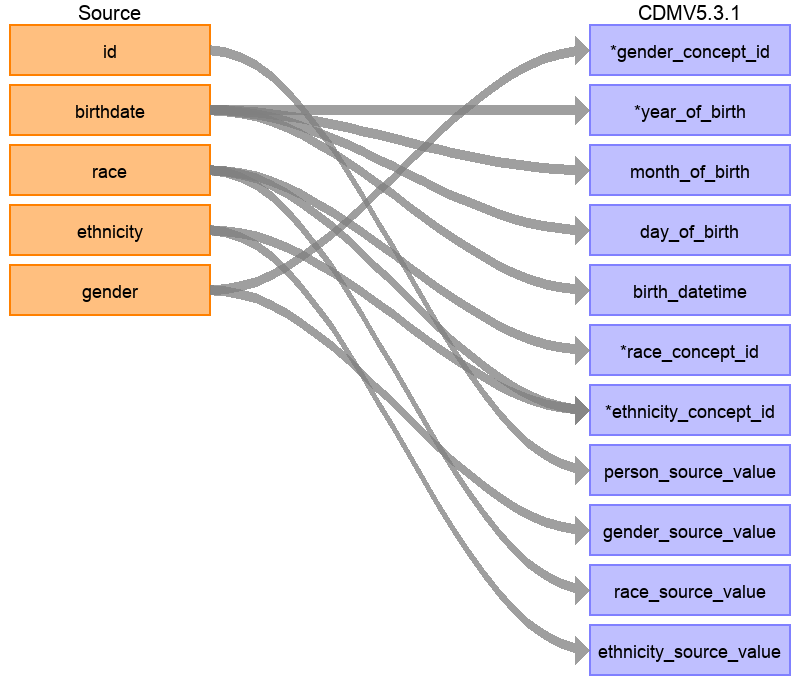
\includegraphics[width=1\linewidth]{images/ExtractTransformLoad/syntheaPersonTable} 

}

\caption{Synthea PatientsテーブルからCDM PERSONテーブルへのマッピング。}\label{fig:syntheaPerson}
\end{figure}

表\ref{tab:syntheaEtlPerson}には、Synthea patientsテーブルをCDM PERSONテーブルに変換するために課されたロジックが示されています。『Destination Field』(目的フィールド)は、CDMのどこにデータがマッピングされるかを示しています。『Source field』(ソースフィールド)は、CDMカラムを埋めるために使用されるソーステーブル(この場合はpatients)のカラムを強調します。最後に、『Logic \& comments』(ロジックとコメント)カラムには、ロジックの説明が記載されています。

表:(#tab:syntheaEtlPerson) Synthea PatientsテーブルをCDM PERSONテーブルに変換するためのETLロジック

\begin{longtable}[]{@{}
  >{\raggedright\arraybackslash}p{(\columnwidth - 4\tabcolsep) * \real{0.3108}}
  >{\raggedright\arraybackslash}p{(\columnwidth - 4\tabcolsep) * \real{0.1351}}
  >{\raggedright\arraybackslash}p{(\columnwidth - 4\tabcolsep) * \real{0.5541}}@{}}
\toprule\noalign{}
\begin{minipage}[b]{\linewidth}\raggedright
目的フィールド
\end{minipage} & \begin{minipage}[b]{\linewidth}\raggedright
ソースフィールド
\end{minipage} & \begin{minipage}[b]{\linewidth}\raggedright
ロジックとコメント
\end{minipage} \\
\midrule\noalign{}
\endhead
\bottomrule\noalign{}
\endlastfoot
PERSON\_ID & & 自動生成。 PERSON\_IDは実装時に生成されます。これは、ソースのid値がvarchar値であり、PERSON\_IDは整数であるためです。 ソースのidフィールドは、その値を保持し、必要に応じてエラーチェックを行うためにPERSON\_SOURCE\_VALUEとして設定されます。 \\
GENDER\_CONCEPT\_ID & gender & 性別が「M」の場合、GENDER\_CONCEPT\_IDは8507、性別が「F」の場合は8532に設定します。不明な性別を持つ行は削除します。これらの2つのコンセプトは、性別ドメインの唯一の標準コンセプトであるため選ばれました。不明な性別の患者を削除するかどうかの決定は、通常、サイトに基づいて行われますが、性別のない人々は分析から除外されるため、削除することを推奨します。 \\
YEAR\_OF\_BIRTH & birthdate & 生年月日から \\
\end{longtable}

\section{ステップ2: コードマッピングの作成}\label{ux30b9ux30c6ux30c3ux30d72-ux30b3ux30fcux30c9ux30deux30c3ux30d4ux30f3ux30b0ux306eux4f5cux6210}

OMOPボキャブラリには時間とともにますます多くのソースコードが追加されています。これは、CDMにデータを変換する際のコーディングシステムが既に含まれており、マッピングされている可能性があることを意味します。含まれているボキャブラリを確認するために、OMOPボキャブラリのVOCABULARYテーブルをチェックしてください。非標準のソースコード(例:ICD-10CMコード)から標準コンセプト(例:SNOMEDコード)へのマッピングを抽出するには、relationship\_id =「Maps to」を持つCONCEPT\_RELATIONSHIPテーブルのレコードを使用できます。例えば、ICD-10CMコード「I21」(「急性心筋梗塞」)の標準コンセプトIDを見つけるためには、次のSQLを使用します:

\begin{Shaded}
\begin{Highlighting}[]
\KeywordTok{SELECT}\NormalTok{ concept\_id\_2 }\KeywordTok{AS}\NormalTok{ standard\_concept\_id}
\KeywordTok{FROM}\NormalTok{ concept\_relationship}
\KeywordTok{INNER} \KeywordTok{JOIN}\NormalTok{ concept }\KeywordTok{AS}\NormalTok{ source\_concept}
  \KeywordTok{ON}\NormalTok{ concept\_id }\OperatorTok{=}\NormalTok{ concept\_id\_1}
\KeywordTok{WHERE}\NormalTok{ concept\_code }\OperatorTok{=} \StringTok{\textquotesingle{}I21\textquotesingle{}}
  \KeywordTok{AND}\NormalTok{ vocabulary\_id }\OperatorTok{=} \StringTok{\textquotesingle{}ICD10CM\textquotesingle{}}
  \KeywordTok{AND}\NormalTok{ relationship\_id }\OperatorTok{=} \StringTok{\textquotesingle{}Maps to\textquotesingle{}}\NormalTok{;}
\end{Highlighting}
\end{Shaded}

\begin{longtable}[]{@{}r@{}}
\toprule\noalign{}
STANDARD\_CONCEPT\_ID \\
\midrule\noalign{}
\endhead
\bottomrule\noalign{}
\endlastfoot
312327 \\
\end{longtable}

残念ながら、ソースデータがボキャブラリに含まれていないコーディングシステムを使用している場合もあります。この場合、ソースコーディングシステムから標準コンセプトへのマッピングを作成する必要があります。コードマッピングは特にソースコーディングシステムに多くのコードが含まれている場合、気が遠くなる作業です。作業を楽にするために以下のことを行うことができます:

\begin{itemize}
\tightlist
\item
  最も頻繁に使用されるコードに焦点を当てる。本当に使用されていないか、ほとんど使用されていないコードに労力を割く価値はありません。
\item
  可能な限り既存の情報を活用する。例えば、多くの国の薬品コーディングシステムはATCにマッピングされています。ATCは多くの目的には詳細でないかもしれませんが、ATCとRxNormのコンセプトの関係を使って適切なRxNormコードを推測することができます。
\item
  Usagiを使用。
\end{itemize}

\subsection{Usagi}\label{usagi}

Usagiはコードマッピングを手動で作成するプロセスを支援するツールです。コード記述のテキスト類似性に基づいたマッピングを提案できます。ソースコードが外国語でしか利用できない場合、Google Translate\footnote{\url{https://translate.google.com/}}は驚くほど良い翻訳を提供することがわかっています。Usagiは自動提案が正しくない場合に適切なターゲットコンセプトを検索する機能を提供します。最終的に、ユーザーはそのマッピングがETLで使用される許可がされていることを示すことができます。UsagiはGitHubで入手可能です\footnote{\url{https://github.com/OHDSI/Usagi}}。 \index{Usagi} \index{source code mapping|see {Usagi}}

\subsubsection{範囲と目的}\label{ux7bc4ux56f2ux3068ux76eeux7684-2}

マッピングが必要なソースコードはUsagiにロードされます(コードが英語でない場合は追加の翻訳列が必要です)。用語の類似性アプローチを使用してソースコードをボキャブラリコンセプトに接続します。ただし、これらのコード接続は手動で見直す必要があり、Usagiはこれを支援するインターフェースを提供します。Usagiはボキャブラリで標準コンセプトとしてマークされているコンセプトのみを提案します。

\subsubsection{プロセス概要}\label{ux30d7ux30edux30bbux30b9ux6982ux8981-2}

このソフトウェアを使用する一般的な手順は次のとおりです:

\begin{enumerate}
\def\labelenumi{\arabic{enumi}.}
\tightlist
\item
  マッピングしたいソースシステムからソースコードをロードします。
\item
  Usagiは用語の類似性アプローチを実行してソースコードをボキャブラリコンセプトにマッピングします。
\item
  Usagiのインターフェースを利用して、自動提案の正しさを確認し、必要に応じて改善します。コードシステムと医療用語に精通した個人によるレビューが推奨されます。
\item
  ボキャブラリのSOURCE\_TO\_CONCEPT\_MAPにマッピングをエクスポートします。
\end{enumerate}

\subsubsection{ソースコードをUsagiにインポート}\label{ux30bdux30fcux30b9ux30b3ux30fcux30c9ux3092usagiux306bux30a4ux30f3ux30ddux30fcux30c8}

ソースコードをCSVまたはExcel (.xlsx) ファイルにエクスポートします。これには、ソースコードと英語のソースコード記述が含まれている必要がありますが、追加の情報(例:投与単位、元の言語の説明(翻訳された場合))も持ち込むことができます。さらに、コードの頻度も持ち込むことが望ましく、これによりどのコードに最も労力をかけるべきかを優先的に決定するのに役立ちます(例:1,000個のソースコードがあっても、システム内で本当に使用されるのは100個だけかもしれません)。英語に翻訳する必要がある場合は、Google Translateを使用します。

注意事項: ソースコードの抽出はドメインごとに分けて行い、1つの大きなファイルにまとめないでください(例:薬剤、処置、コンディション、観察)。

ソースコードはFile → Import codesメニューからUsagiにロードされます。ここでは「Import codes \ldots」が表示される(図\ref{fig:usagiImport})。この図では、ソースコード用語がオランダ語で、英語に翻訳されたものも含まれています。Usagiは英語の翻訳を利用して標準ボキャブラリにマッピングします。

\begin{figure}

{\centering 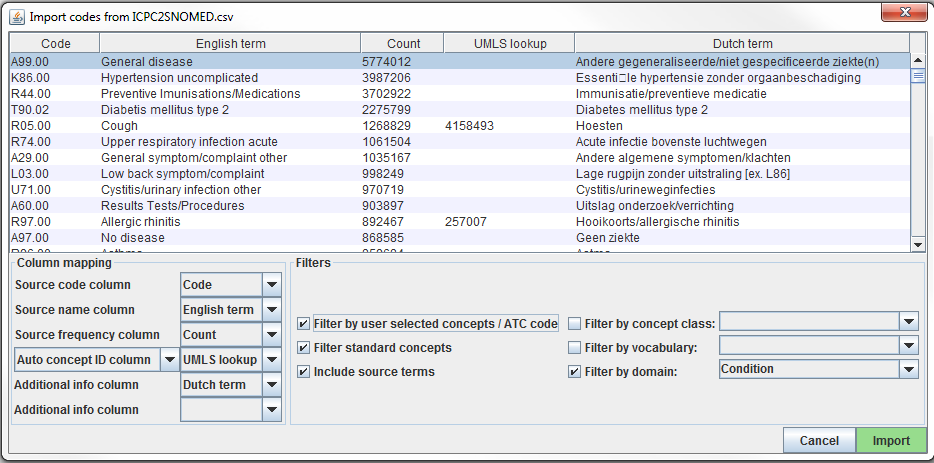
\includegraphics[width=1\linewidth]{images/ExtractTransformLoad/usagiImport} 

}

\caption{Usagiコード入力画面。}\label{fig:usagiImport}
\end{figure}

「Column mapping」セクション(左下)では、インポートされたテーブルをUsagiに対してどのように使用するかを定義します。ドロップダウンメニューにマウスを合わせると、それぞれの列の定義が表示されるポップアップが表示されます。Usagiは「Additional info」列をソースコードとボキャブラリコンセプトコードを関連付けるための情報として使用しませんが、この追加の情報はソースコードマッピングを確認する個々人を支援するのに役立ちますので、含めるべきです。

また、「Filters」セクション(右下)で、Usagiがマッピングする際の制限を設定できます。例えば、図\ref{fig:usagiImport}では、ユーザーはソースコードをConditionドメインのコンセプトにマッピングしています。デフォルトでは、Usagiは標準コンセプトにしかマッピングしませんが、「Filter standard concepts」をオフにすると、Usagiは分類コンセプトも考慮します。各フィルターについて詳細を知るためには、異なるフィルターにマウスをホバーさせてください。

特別なフィルターとして「Filter by automatically selected concepts / ATC code」があります。制限する情報がある場合、Auto concept ID列(セミコロンで区切られた)にCONCEPT\_IDsまたはATCコードのリストを提供することで検索を制限できます。例えば、薬剤の場合、既に各薬剤にATCコードが割り当てられているかもしれません。ATCコードは単一のRxNorm薬剤コードを特定しませんが、ボキャブラリ内のATCコードに該当するコンセプトのみを検索することで検索範囲を制限するのに役立ちます。ATCコードを使用するには、以下の手順に従います:

\begin{enumerate}
\def\labelenumi{\arabic{enumi}.}
\tightlist
\item
  Column mapping部で、``Auto concept ID column''から''ATC column''に切り替える
\item
  Column mapping部で、ATCコードの列を''AT
\end{enumerate}

\section{ステップ 3: ETLの実装}\label{ux30b9ux30c6ux30c3ux30d7-3-etlux306eux5b9fux88c5}

デザインとコードマッピングが完了したら、ETLプロセスをソフトウェアで実装することができます。ETLのデザイン段階では、ソースデータとCDMに詳しい人が共同で作業することをおすすめしました。同様に、ETLを実装する際には、大量のデータを扱う経験があり、ETLの実装経験がある人を使うことが望ましいです。これは、あなたのグループ外の個人と協力することや、実装を担当する技術顧問を雇うことを意味するかもしれません。また、これは一度きりの費用ではないことにも注意が必要です。今後もETLの維持と運用を担当するために、少なくとも一部の時間を捧げる個人やチームがいることが望ましいです(詳細はセクション \ref{CDMandETLMaintenance} を参照してください)。

実装の具体的な内容はサイトごとに異なり、インフラ、データベースの規模、ETLの複雑さ、利用可能な技術専門知識など多くの要因に依存します。そのため、OHDSIコミュニティはETLの最適な実装方法について正式な推奨を行っていません。シンプルなSQLビルダー、SAS、C\#、Java、およびKettleを使用するグループもいます。それぞれに長所と短所があり、技術に精通している人がいなければどれも使えません。

様々なETLの例をいくつか挙げます(複雑さの順に記載):\index{ETL!implementations}

\begin{itemize}
\tightlist
\item
  ETL-Synthea - Syntheaデータベースを変換するために書かれたSQLビルダー

  \begin{itemize}
  \tightlist
  \item
    \url{https://github.com/OHDSI/etl-synthea}
  \end{itemize}
\item
  ETL-CDMBuilder - 複数のデータベースを変換するためにデザインされた.NETアプリケーション

  \begin{itemize}
  \tightlist
  \item
    \url{https://github.com/OHDSI/etl-cdmbuilder}
  \end{itemize}
\item
  ETL-LambdaBuilder - AWS lambda機能を使用するビルダー

  \begin{itemize}
  \tightlist
  \item
    \url{https://github.com/OHDSI/etl-lambdabuilder}
  \end{itemize}
\end{itemize}

複数回の独立した試みの後、ユーザーフレンドリーな''究極の''ETLツールの開発を断念しました。このようなツールはETLの80\%にはうまく機能しますが、残りの20\%のETLには、ソースデータベース固有の低レベルのコードを書く必要があります。

技術者が実装を開始する準備ができたら、ETLデザイン文書を彼らと共有するべきです。ドキュメントには開発を開始するための十分な情報が含まれているはずですが、開発プロセス中にETLデザイン者が質問に応じることができるようにすることが重要です。デザイン者には明確な論理も、データやCDMに不慣れな実装者にはわかりにくいことがあります。実装フェーズはチーム全体の努力として維持されるべきです。実装者とデザイン者の間で、CDMの作成とテストのプロセスを繰り返し行い、両グループがすべての論理が正しく実行されたことに同意するまで進行することが受け入れられた慣行とされています。

\section{ステップ 4: 品質管理}\label{ux30b9ux30c6ux30c3ux30d7-4-ux54c1ux8ceaux7ba1ux7406}

抽出、変換、ロードプロセスでは品質管理が反復的です。一般的なパターンは、ロジックの記述-\textgreater ロジックの実装-\textgreater ロジックのテスト-\textgreater ロジックの修正・記述です。CDMをテストする方法はいくつもありますが、以下は何年にもわたるETL実装を通じてコミュニティ全体で開発された推奨ステップです。 \index{ETL!quality control}

\begin{itemize}
\tightlist
\item
  ETLデザイン文書、コンピュータコード、およびコードマッピングのレビュー。1人の人がミスをすることは常にあるので、必ず他の1人以上が行ったことをレビューするべきです。

  \begin{itemize}
  \tightlist
  \item
    コンピュータコードにおける最大の問題は、ネイティブデータのソースコードが標準コンセプトにどのようにマッピングされるかに起因します。特に日付特有のコード(NDCなど)の場合、マッピングは難しくなることがあります。どの領域でもマッピングが行われる場合は、正しいソースボキャブラリが適切なコンセプトIDに変換されているかを必ず再確認してください。
  \end{itemize}
\item
  ソースデータとターゲットデータのサンプルに関する情報を手動で比較します。

  \begin{itemize}
  \tightlist
  \item
    最大のユニークなレコード数を持つ理想的な1人のデータを追跡するのが役立つことがあります。1人のデータを追跡することで、CDMのデータが合意されたロジックに基づいて期待されるように見えない場合に問題が浮かび上がります。
  \end{itemize}
\item
  ソースデータとターゲットデータの全体的なカウントを比較します。

  \begin{itemize}
  \tightlist
  \item
    特定の問題にどのように対処するかによって、カウントに期待される差異があるかもしれません。たとえば、NULL性別の人々を解析から完全に除外する協力者がいます。また、CDMの受診期間がネイティブデータの受診やエンカウンターと異なるように構築されることもあります。そのため、ソースデータとCDMデータ間の全体的なカウントを比較する際には、これらの違いに留意し、期待する必要があります。
  \end{itemize}
\item
  ソースデータで既に行われた研究をCDMバージョンで再現します。

  \begin{itemize}
  \tightlist
  \item
    これはソースデータとCDMバージョンとの間の主要な違いを理解するための良い方法ですが、少し時間がかかります。
  \end{itemize}
\item
  ETLで対処する必要があるソースデータのパターンを再現するユニットテストを作成します。たとえば、性別情報のない患者が削除されるべき場合、性別がない個人のユニットテストを作成し、ビルダーがどのように処理するかを評価します。

  \begin{itemize}
  \tightlist
  \item
    ユニットテストは、ETL変換の品質と精度を評価する際に非常に便利です。通常、変換元データの構造を模倣する非常に小さいデータセットを作成します。このデータセット内の各個人またはレコードは、ETL文書に記載されている特定のロジックをテストします。この方法では、問題を特定し、失敗したロジックを特定するのが簡単になります。小さいサイズはコンピュータコードの実行が非常に速くなり、反復とエラーの特定を迅速に行えます。
  \end{itemize}
\end{itemize}

これらは、ETLの観点から品質管理にアプローチする高レベルの方法です。OHDSIコミュニティ内で進行中のデータ品質への取り組みの詳細については、Chapter \ref{DataQuality} を参照してください。

\section{ETLの規約とTHEMIS}\label{etlux306eux898fux7d04ux3068themis}

データをCDMに変換するグループが増えるにつれ、特定の状況でETLがどのように対処すべきかを指定する必要があることが明らかになりました。たとえば、出生年が欠けている個人記録の場合、ETLはどうすべきでしょうか?CDMの目標はヘルスケアデータを標準化することですが、各グループが特定のデータシナリオを異なる方法で処理すると、ネットワーク全体でデータを体系的に使用することが難しくなります。

OHDSIコミュニティは、一貫性を向上させるために慣行を文書化し始めました。OHDSIコミュニティが合意したこれらの定義された慣行は、CDM Wikiで見つけることができます\footnote{\url{https://github.com/OHDSI/CommonDataModel/wiki}}。各CDMテーブルには、ETLをデザインする際に参照できる独自の慣行セットがあります。たとえば、出生月や日が欠けている個人は許可されますが、出生年が欠けている場合、その個人は削除する必要があります。ETLをデザインする際には、コミュニティと一貫性のあるデザイン決定を行うために参考文献を参照してください。

すべてのデータシナリオを文書化し、発生した場合に何をするかをドキュメント化することは不可能ですが、共通のシナリオを文書化しようとしているOHDSIの作業グループがあります。THEMIS\footnote{\url{https://github.com/OHDSI/Themis}}は、コミュニティ内で慣行を収集し、それを明確にし、コミュニティと共有し、最終的な慣行をCDM Wikiに文書化する個人で構成されています。Themisは、古代ギリシャの神であり、秩序、公平さ、法、自然法、慣習を司るタイタネスであり、このグループの任務にふさわしいものでした。ETLを実行する際に、どのように処理すべきか判断に迷うシナリオがあった場合、THEMISはそのシナリオについてOHDSIフォーラムに質問を投げかけることをお勧めします\footnote{\url{http://forums.ohdsi.org/}}。おそらく、質問がある場合、他のコミュニティのメンバーも同じ質問を抱えている可能性があります。THEMISはこれらの議論、作業グループの会議、フェイス・トゥ・フェイスのディスカッションなどを利用して、他に文書化する必要がある慣行について情報を収集します。

\section{CDMおよびETLのメンテナンス}\label{CDMandETLMaintenance}

ETLをデザインし、マッピングを作成し、ETLを実装し、品質管理措置を構築することは容易な作業ではありません。残念ながら、この努力はそこで終わりではありません。最初のCDMが構築されると、ETLメンテナンスのサイクルが継続的に行われます。メンテナンスが必要となる一般的なトリガーは以下の通りです:ソースデータの変更、ETLのバグ、新しいOMOPボキャブラリのリリース、またはCDM自体の変更や更新です。これらのトリガーが発生すると、ETLドキュメント、ETLを実行するソフトウェアプログラミング、テストケースや品質管理の更新が必要になる場合があります。

医療データソースは常に変化し続けることがよくあります。新しいデータが利用可能になるかもしれません(例:データに新しい列が追加される)。存在しなかった患者のシナリオが突然現れるかもしれません(例:生まれる前に死亡記録がある新しい患者)。データの理解が向上するかもしれません(例:保険請求データの処理の方法により、入院出産に関する記録の一部が外来として処理されること)。すべてのソースデータの変更がETL処理の変更を引き起こすわけではありませんが、最低限、ETL処理を中断する変更は対処する必要があります。

バグが見つかった場合、それに対処する必要があります。しかし、すべてのバグが同じ重要性を持っているわけではないことを忘れないでください。例えば、COSTテーブルではcost列が整数に丸められていたとしましょう(例:ソースデータに\$3.82があったのに、CDMで\$4.00になっている)。データを使用して主に患者の薬剤曝露やコンディションの特性評価を行う研究者が多い場合、このようなバグは重要ではなく、将来的に対処することができます。しかし、データを使用する主要な研究者に健康経済学者も含まれていた場合、これは直ちに対処する必要がある重大なバグとなります。

OMOPボキャブラリもまた、ソースデータと同様に常に変化しています。実際、ボキャブラリは1ヶ月に何度も更新されることがあります。各CDMは特定のボキャブラリバージョンで実行されており、新しい改善されたボキャブラリで実行すると、標準化されたボキャブラリにソースコードがマッピングされる方法が変わる可能性があります。ボキャブラリの違いはしばしば些細なものですが、新しいボキャブラリがリリースされるたびに新しいCDMを構築することは不要です。しかし、年間に1回か2回程度、新しいボキャブラリを採用することが良いとされています。この場合、CDMを再処理する必要があります。新しいバージョンのボキャブラリの変更がETLコード自体の更新を必要とすることはまれです。

CDMまたはETLのメンテナンスが必要となる最後のトリガーは、共通データモデル自体の更新時です。コミュニティが成長し、新しいデータ要件が見つかると、これがCDMに追加データを保存することにつながるかもしれません。これは、以前はCDMに保存されていなかったデータが新しいCDMバージョンに保存場所を持つ可能性があることを意味します。既存のCDM構造の変更は頻繁ではありませんが、可能性はあります。例えば、CDMが元のDATEフィールドからDATETIMEフィールドを採用したことで、ETL処理にエラーが発生する可能性があります。CDMバージョンは頻繁にはリリースされず、サイトは移行するタイミングを選択できます。

\section{ETLに関する最終的な考察}\label{etlux306bux95a2ux3059ux308bux6700ux7d42ux7684ux306aux8003ux5bdf}

ETLプロセスにはさまざまな理由で困難があります。その中でも、私たちが処理しているソースデータの独自性により、「1つの解決策がすべてに適合する」という解決策を作成するのが難しいことが最大の理由の1つです。しかし、過去数年で以下のような貴重な教訓を得ました。

\begin{itemize}
\tightlist
\item
  80/20のルール。可能な限り、ソースコードを手動でコンセプトセットにマッピングするのに過度に時間を費やさないようにしましょう。理想的には、大多数のデータをカバーするソースコードをマッピングしてください。これで十分であり、将来のユースケースに基づいて残りのコードに対処することができます。
\item
  研究の品質に見合わないデータを失うことを恐れなくても良い。それらはしばしば分析を開始する前に破棄されるレコードであり、私たちはETLプロセス中にそれらを削除します。
\item
  CDMはメンテナンスが必要です。ETLが完了したからといって、再び触らないということではありません。生データが変更されるかもしれませんし、コードにバグがあるかもしれません。新しいボキャブラリやCDMの更新があるかもしれません。これらの変更に対応するためのリソースを計画しておくことで、ETLが常に最新の状態に保たれるようにしましょう。
\item
  OHDSI CDMの開始、データベースの変換、分析ツールの実行のサポートが必要な場合は、実施者フォーラム\footnote{\url{https://forums.ohdsi.org/c/implementers}}をご覧ください。
\end{itemize}

\section{まとめ}\label{ux307eux3068ux3081-4}

\begin{rmdsummary}
\begin{itemize}
\item
  ETLにアプローチするための一般的に合意されたプロセスが存在します

  \begin{itemize}
  \tightlist
  \item
    データ専門家とCDM専門家が協力してETLをデザイン
  \item
    医療知識を持つ人々がコードマッピングを作成
  \item
    技術者がETLを実装
  \item
    すべての関係者が品質管理に関与
  \end{itemize}
\item
  OHDSIコミュニティはこれらのステップを促進するためにツールを開発しており、これらは自由に使用できます
\item
  ガイドとして使用できる多くのETL例や合意された慣習があります
\end{itemize}
\end{rmdsummary}

\section{演習}\label{ux6f14ux7fd2-1}

\begin{exercise}
\protect\hypertarget{exr:exerciseEtl1}{}\label{exr:exerciseEtl1}

ETLプロセスのステップを適切な順序に並べてください:

\begin{enumerate}
\def\labelenumi{\Alph{enumi})}
\tightlist
\item
  データ専門家とCDM専門家が協力してETLをデザイン
\item
  技術者がETLを実装
\item
  医療知識を持つ人々がコードマッピングを作成
\item
  すべての関係者が品質管理に関与
\end{enumerate}

\end{exercise}

\begin{exercise}
\protect\hypertarget{exr:exerciseEtl2}{}\label{exr:exerciseEtl2}

選択したOHDSIリソースを使用して、表\ref{tab:exercisePersonTable}に示すPERSONレコードに関する4つの問題点を指摘してください(表はスペースのため省略されています):

表: \label{tab:exercisePersonTable} PERSONテーブル。

\begin{longtable}[]{@{}ll@{}}
\toprule\noalign{}
列 & 値 \\
\midrule\noalign{}
\endhead
\bottomrule\noalign{}
\endlastfoot
PERSON\_ID & A123B456 \\
GENDER\_CONCEPT\_ID & 8532 \\
YEAR\_OF\_BIRTH & NULL \\
MONTH\_OF\_BIRTH & NULL \\
DAY\_OF\_BIRTH & NULL \\
RACE\_CONCEPT\_ID & 0 \\
ETHNICITY\_CONCEPT\_ID & 8527 \\
PERSON\_SOURCE\_VALUE & A123B456 \\
GENDER\_SOURCE\_VALUE & F \\
RACE\_SOURCE\_VALUE & WHITE \\
ETHNICITY\_SOURCE\_VALUE & 提供されていない \\
\end{longtable}

\end{exercise}

\begin{exercise}
\protect\hypertarget{exr:exerciseEtl3}{}\label{exr:exerciseEtl3}VISIT\_OCCURRENCEレコードを生成してみましょう。以下はSyntheaのために書かれた一部のロジックです:
PATIENT、START、ENDを昇順で並べ替えます。その後、PERSON\_IDごとに、前の行のENDと次の行のSTARTの間に1日以内の時間がある限り、請求行をまとめます。まとめられた入院請求ごとに1つの入院受診期間と見なし、以下を設定します:

\begin{itemize}
\tightlist
\item
  MIN(START)をVISIT\_START\_DATEとして設定
\item
  MAX(END)をVISIT\_END\_DATEとして設定
\item
  ``IP''をPLACE\_OF\_SERVICE\_SOURCE\_VALUEとして設定
\end{itemize}

ソースデータに図\ref{fig:exerciseSourceData}に示されるような訪問セットがある場合、CDMで生成されるVISIT\_OCCURRENCEレコードはどのようになると予想しますか?
\end{exercise}

\begin{figure}

{\centering 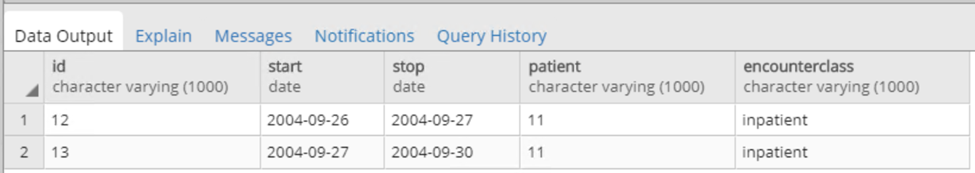
\includegraphics[width=1\linewidth]{images/ExtractTransformLoad/exerciseSourceData} 

}

\caption{例のソースデータ。}\label{fig:exerciseSourceData}
\end{figure}

提案された回答は付録\ref{Etlanswers}に見つけることができます。

\chapter*{第7章 --翻訳作業中-- データ解析}\label{ux7b2c7ux7ae0-ux7ffbux8a33ux4f5cux696dux4e2d-ux30c7ux30fcux30bfux89e3ux6790}
\addcontentsline{toc}{chapter}{第7章 --翻訳作業中-- データ解析}

\chapter{データ解析の使用例}\label{DataAnalyticsUseCases}

\emph{チャプターリード: David Madigan}

OHDSIのコラボレーションは、通常、保険請求データベースや電子健康記録データベースの形態で実世界のヘルスケアデータから信頼できるエビデンスを生成することに焦点を当てています。OHDSIが焦点を当てる使用例は、以下の3つの主要なカテゴリに分かれます:

\begin{itemize}
\tightlist
\item
  特徴分析
\item
  集団レベルの推定
\item
  患者レベルの予測
\end{itemize}

これらを以下で詳細に説明します。すべての使用例について、生成するエビデンスはデータの限界を継承します; これらの限界については、エビデンスの質に関する本のセクション(Chapters \ref{EvidenceQuality} - \ref{MethodValidity})で詳しく議論します。

\section{特徴分析}\label{ux7279ux5fb4ux5206ux6790}

\index{characterization}

特徴分析は次の質問に答えようとします

\begin{quote}
彼らに何が起こったのか?
\end{quote}

データを使用して、コホート全体やデータベース全体における人物の特性、ヘルスケアの実践、およびこれらの変化を時間とともに研究する質問に答えることができます。

データが答えを提供できる質問の例は次のとおりです:

\begin{itemize}
\tightlist
\item
  新たに心房細動と診断された患者のうち、何人がワルファリンの処方を受けるか?
\item
  股関節置換術を受けた患者の平均年齢は?
\item
  65歳以上の患者の肺炎の発生率は?
\end{itemize}

典型的な特性の評価は次のように定式化されます:

\begin{itemize}
\tightlist
\item
  何人の患者が\ldots?
\item
  どのくらいの頻度で\ldots?
\item
  何割の患者が\ldots?
\item
  ラボの数値の分布はどのようになっているか\ldots?
\item
  患者のHbA1cレベルは\ldots?
\item
  患者のラボ値は\ldots?
\item
  患者の曝露期間の中央値は\ldots?
\item
  時間の経過に伴う傾向は?
\item
  これらの患者が使用している他の薬剤は何か?
\item
  併用療法は?
\item
  \ldots の症例が十分にあるか?
\item
  Xを研究することが可能か?
\item
  \ldots の人口統計学は?
\item
  \ldots のリスク要因は?(特定のリスク要因を識別する場合、推定か予測)
\item
  \ldots の予測因子は?
\end{itemize}

望ましい出力は次のとおりです:

\begin{itemize}
\tightlist
\item
  カウントまたはパーセンテージ
\item
  平均
\item
  記述統計
\item
  発生率
\item
  有病率
\item
  コホート
\item
  ルールベースのフェノタイプ
\item
  薬剤利用
\item
  病気の自然史
\item
  アドヒアランス
\item
  共病プロファイル
\item
  治療パスウェイ
\item
  治療ライン
\end{itemize}

\section{集団レベルの推定}\label{ux96c6ux56e3ux30ecux30d9ux30ebux306eux63a8ux5b9a}

\index{population-level estimation}

限られた範囲で、データはヘルスケア介入の効果に関する因果推論をサポートすることができ、次の質問に答えます

\begin{quote}
因果効果は何か?
\end{quote}

行動の結果を理解するために因果効果を理解したいです。例えば、特定の治療を行うことに決めた場合、将来に何が起こるかがどのように変わるかを理解したいです。

データが答えを提供できる質問の例は次のとおりです:

\begin{itemize}
\tightlist
\item
  新たに心房細動と診断された患者において、治療開始後最初の1年間で、ワルファリンはダビガトランよりも多くの主要な出血を引き起こすか?
\item
  メトホルミンの下痢に対する因果効果は年齢によって異なるか?
\end{itemize}

典型的な集団レベルの効果推定の質問は次のように定式化されます:

\begin{itemize}
\tightlist
\item
  \ldots の効果は?
\item
  介入\ldots を行った場合は?
\item
  どの治療がより良いか?
\item
  Yに対するXのリスクは?
\item
  \ldots のイベントまでの時間は?
\end{itemize}

望ましい出力は次のとおりです:

\begin{itemize}
\tightlist
\item
  相対リスク
\item
  ハザード比
\item
  オッズ比
\item
  平均治療効果
\item
  因果効果
\item
  関連
\item
  相関
\item
  安全監視
\item
  比較の効果
\end{itemize}

\section{患者レベルの予測}\label{ux60a3ux8005ux30ecux30d9ux30ebux306eux4e88ux6e2c}

\index{patient-level prediction}

データベースに収集された患者の健康履歴に基づいて、将来の健康イベントに関する患者レベルの予測を行い、次の質問に答えます

\begin{quote}
私には何が起こるのか?
\end{quote}

データが答えを提供できる質問の例は次のとおりです:

\begin{itemize}
\tightlist
\item
  新たに重度うつ病と診断された特定の患者について、診断後最初の1年間でその患者が自殺を試みる確率は?
\item
  新たに心房細動と診断され、ワルファリンで治療を開始した特定の患者について、治療開始後最初の1年間で脳梗塞を発症する確率は?
\end{itemize}

典型的な患者レベルの予測の問題は次のように定式化されます:

\begin{itemize}
\tightlist
\item
  この患者が\ldots する可能性は?
\item
  \ldots の候補は誰か?
\end{itemize}

望ましい出力は次のとおりです:

\begin{itemize}
\tightlist
\item
  個人の確率
\item
  予測モデル
\item
  高リスク/低リスクグループ
\item
  確率的表現型
\end{itemize}

集団レベルの推定と患者レベルの予測はある程度重なることがあります。例えば、重要な予測の使用例として、薬剤Aが処方された場合の特定患者に対する結果を予測し、薬剤Bが処方された場合の同じ結果を予測するというものがあります。現実にはこれらの薬剤のうちどちらか一方の薬(例えば薬剤A)が実際に処方されるため、Aの治療後の結果が実際にどうなるかを観察することができます。薬剤Bが処方されなかったため、Bでの治療後のアウトカムは予測可能ではありますが、「反事実」であり、実際には観察されません。これらの予測タスクの各々は患者レベルの予測に該当します。しかし、アウトカムの差(または比)は単位レベルの\emph{因果}効果であり、因果効果推定方法を使用して推定する必要があります。

\begin{rmdimportant}
人々は予測モデルを因果モデルとして誤解釈する傾向があります。しかし、予測モデルは相関のみを示すことができ、因果関係を示すことはできません。例えば、糖尿病薬剤の使用は心筋梗塞(MI)の強力な予測因子であるかもしれませんが、それは糖尿病がMIの強力なリスク要因だからです。しかし、それは糖尿病薬剤を中止することでMIを予防できるということを意味しません!
\end{rmdimportant}

\section{高血圧における使用例}\label{ux9ad8ux8840ux5727ux306bux304aux3051ux308bux4f7fux7528ux4f8b}

あなたは、ACE阻害薬単独療法とチアジド系利尿薬単独療法が高血圧の初期治療として急性心筋梗塞や血管浮腫のアウトカムに及ぼす影響を研究することに興味がある研究者です。OHDSIの文献に基づいて、集団レベルの効果推定の質問をしていることを理解していますが、まず、この特定の治療に関する特性評価を行うための準備を行う必要があります。

\subsection{特性の評価に関する質問}\label{ux7279ux6027ux306eux8a55ux4fa1ux306bux95a2ux3059ux308bux8ceaux554f}

急性心筋梗塞は高血圧患者に発生する可能性のある心血管合併症であり、高血圧に対する効果的な治療法はリスクを軽減するべきです。血管浮腫はACE阻害薬の既知の副作用であり、稀であるが潜在的に深刻です。あなたは、対象の曝露(ACE阻害薬の新規使用者およびチアジド系利尿薬の新規使用者)のコホートを作成することから始めます(Chapter \ref{Cohorts}を参照)。曝露集団のベースライン特性を要約するための特性評価(Chapter \ref{Characterization}を参照)解析を実行し、人口統計学的特性、併存疾患、および併用薬を含みます。この曝露集団内で選択されたアウトカムの発生率を推定するための別の特性評価を実行します。ここで、「ACE阻害薬およびチアジド系利尿薬に曝露された期間に急性心筋梗塞および血管浮腫がどのくらいの頻度で発生するか?」という質問をします。これらの特性評価により、集団レベルの効果推定研究を実施することの実行可能性を評価し、2つの治療グループが比較可能かどうかを評価し、患者の治療選択を予測する`リスク因子'を特定することができます。

\subsection{集団レベルの推定問題}\label{ux96c6ux56e3ux30ecux30d9ux30ebux306eux63a8ux5b9aux554fux984c}

集団レベルの効果推定研究(Chapter \ref{PopulationLevelEstimation}を参照)は、急性心筋梗塞と血管浮腫のアウトカムに対するACE阻害薬対チアジド導入治療の相対リスクを推定します。ここで、研究診断および陰性対照を通じて、平均治療効果の信頼できる推定を生成できるかどうかをさらに評価します。

\subsection{患者レベルの予測問題}\label{ux60a3ux8005ux30ecux30d9ux30ebux306eux4e88ux6e2cux554fux984c}

曝露の因果効果とは独立して、アウトカムのリスクが最も高い患者を特定しようとすることにも興味があります。これは患者レベルの予測問題です(Chapter \ref{PatientLevelPrediction}を参照)。ここで、ACE阻害薬の新規使用者の中で、治療開始後の1年間に急性心筋梗塞を発症するリスクが最も高い患者を評価する予測モデルを開発します。このモデルにより、ACEを初めて処方された患者について、その病歴から観察されたイベントに基づき、次の1年間でAMIを経験する確率を予測することができます。

\section{観察研究の限界}\label{ux89b3ux5bdfux7814ux7a76ux306eux9650ux754c}

\index{観察研究の限界}

OHDSIデータベースでは回答できない重要な医療上の問題が多く存在します。これらには以下が含まれます:

\begin{itemize}
\tightlist
\item
  プラセボと比較した介入の因果効果。治療と非治療を比較する因果効果を考えることは可能な場合もありますが、プラセボ治療と比較することはできません。
\item
  市販薬に関連するすべてのこと。
\item
  多くのアウトカムやその他の変数は、ほとんど記録されていないか、まばらにしか記録されていません。これには、死亡率、行動アウトカム、ライフスタイル、社会経済的地位が含まれます。
\item
  患者は体調が悪いときにしか医療システムを利用しない傾向があるため、治療の利益を測定することが困難です。
\end{itemize}

\subsection{誤ったデータ}\label{ux8aa4ux3063ux305fux30c7ux30fcux30bf}

OHDSIデータベースに記録されている臨床データは、臨床現実から逸脱することがあります。例えば、患者の記録に心筋梗塞のコードが含まれているが、実際には心筋梗塞を経験していない場合があります。同様に、検査値が誤っている場合や、処置の誤ったコードがデータベースに現れることもあります。\ref{DataQuality}および\ref{ClinicalValidity}の各章でこれらの問題について議論し、できる限り多くのこれらの問題を特定して修正するための良い実践方法を紹介しています。それにもかかわらず、誤ったデータはある程度残り続け、その後の分析の妥当性を損なう可能性があります。データの誤りを考慮した統計推論の調整に焦点を当てた文献は豊富であり、例えば@fuller2009measurementを参照してください。

\subsection{欠損データ}\label{ux6b20ux640dux30c7ux30fcux30bf}

\index{欠損データ}

OHDSIデータベースにおける欠損は微妙な課題を呈します。データベースに記録されるべき健康イベント(例:処方、検査値など)が記録されていない場合、それは「欠損」しています。統計学の文献では、「完全にランダムに欠損している」、「ランダムに欠損している」、および「非ランダムに欠損している」などの欠損のタイプを区別し、\href{mailto:それらのタイプに対処する方法の複雑さを増す方法を試みます@perkins2017principled}{\nolinkurl{それらのタイプに対処する方法の複雑さを増す方法を試みます@perkins2017principled}}。 はこのトピックに関する有用な入門書を提供しています。

\section{まとめ}\label{ux307eux3068ux3081-5}

\begin{rmdsummary}
\begin{itemize}
\item
  観察研究では、3つの大きな使用例のカテゴリーを区別します。
\item
  \textbf{特性の評価}は「彼らに何が起こったか?」という質問に答えようとします。
\item
  \textbf{集団レベルの推定}は「因果効果は何か?」という質問に答えようとします。
\item
  \textbf{患者レベルの予測}は「私には何が起こるか?」という質問に答えようとします。
\item
  予測モデルは因果モデルではありません。強力な予測因子に介入しても結果に影響を与える理由はありません。
\item
  観察医療データを使用して回答できない質問があります。
\end{itemize}
\end{rmdsummary}

\section{演習}\label{ux6f14ux7fd2-2}

\begin{exercise}
\protect\hypertarget{exr:exerciseUseCases1}{}\label{exr:exerciseUseCases1}

これらの質問はどの使用例カテゴリーに属しますか?

\begin{enumerate}
\def\labelenumi{\arabic{enumi}.}
\item
  最近NSAIDsに曝露された患者の消化管(GI)出血率を計算します。
\item
  基本的な特徴に基づいて、特定の患者が次の年にGI出血を経験する確率を計算します。
\item
  セレコキシブと比較してジクロフェナクによるGI出血のリスク増加を推定します。
\end{enumerate}

\end{exercise}

\begin{exercise}
\protect\hypertarget{exr:exerciseUseCases2}{}\label{exr:exerciseUseCases2}ジクロフェナクと非曝露(プラセボ)を比較してGI出血のリスク増加を推定したいと考えています。これは観察医療データを使用して行うことができますか?
\end{exercise}

推奨される解答は、Appendix \ref{UseCasesanswers}にあります。

\chapter{第8章 --翻訳作業中-- OHDSI 分析ツール}\label{OhdsiAnalyticsTools}

\emph{チャプターLead: Martijn Schuemie \& Frank DeFalco}

OHDSIは、患者レベルの観察データに対するさまざまなデータ分析のユースケースをサポートするための幅広いオープンソースツールを提供しています。これらのツールの共通点は、すべてCDM(共通データモデル)を使用して1つ以上のデータベースと対話できる点です。さらに、これらのツールはさまざまなユースケースに対して分析を標準化します。一から始める必要はなく、標準テンプレートに入力することで分析を実装できます。これにより、分析が容易になり、再現性と透明性が向上します。例として、発生率を計算する方法は無数にあるように見えますが、OHDSIツールではいくつかの選択肢で指定でき、同じ選択肢を選んだ人は同じ方法で発生率を計算します。

この章では、最初に分析を実装するさまざまな方法を説明し、分析が使用する戦略について述べます。次に、さまざまなOHDSIツールとそれらがどのようにさまざまなユースケースに適合するかをレビューします。

\section{分析の実装}\label{analysisImplementation}

図\ref{fig:implementations}は、CDMを使用してデータベースに対して研究を実装するために選択できるさまざまな方法を示しています。 \index{analysis implementation}

\begin{figure}

{\centering 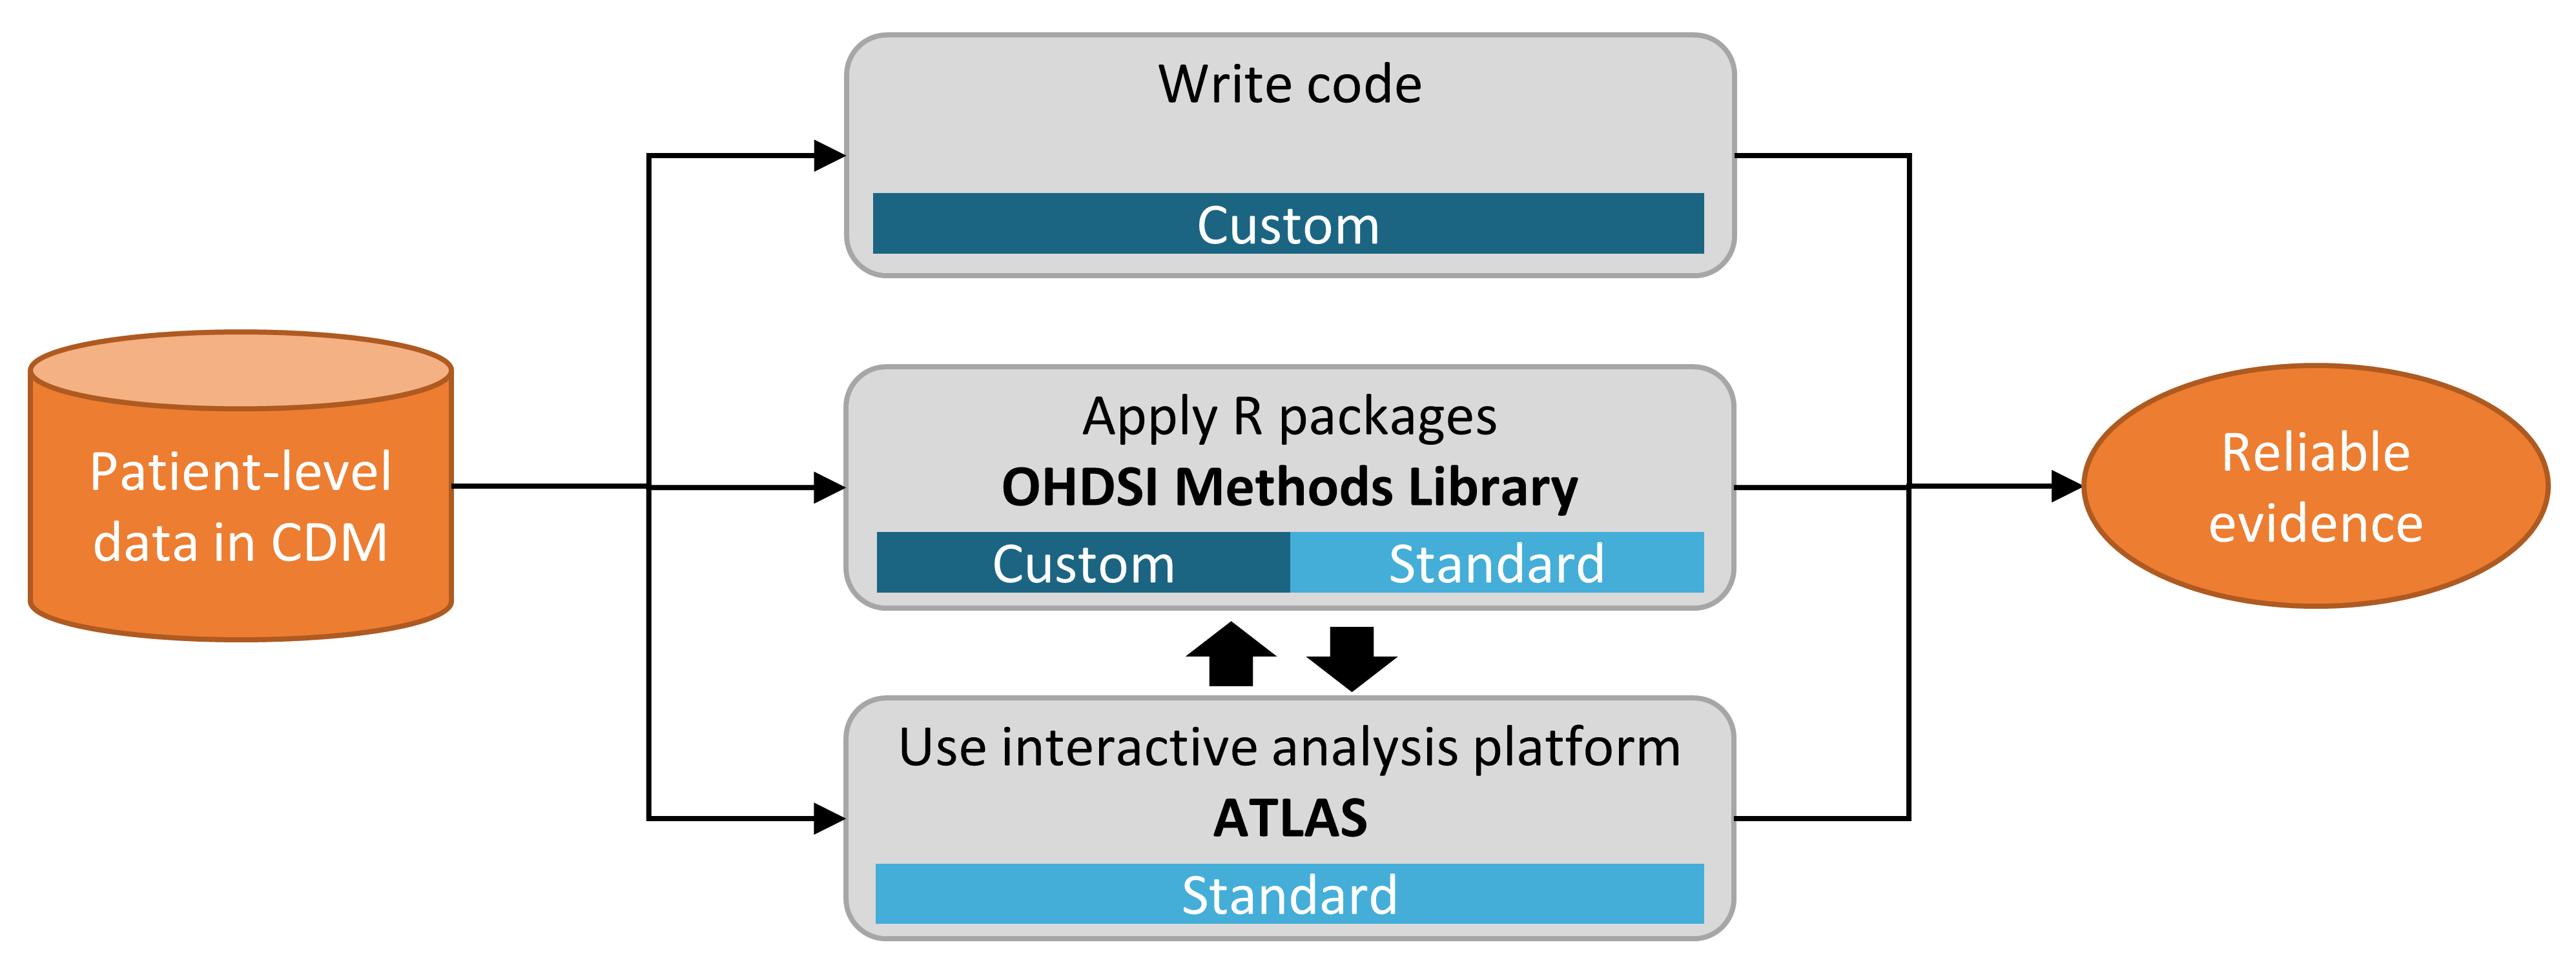
\includegraphics[width=0.9\linewidth]{images/OhdsiAnalyticsTools/implementations} 

}

\caption{CDMのデータに対する分析を実装するさまざまな方法。}\label{fig:implementations}
\end{figure}

研究を実装するための主なアプローチは3つあります。最初の方法は、OHDSIが提供するツールを一切使用しないカスタムコードを作成することです。たとえば、R、SAS、またはその他の言語でゼロから分析を作成することができます。これにより最大の柔軟性が得られ、特定の分析がツールでサポートされていない場合は唯一の選択肢となるかもしれません。しかし、この方法は多くの技術的スキル、時間、および努力を必要とし、分析が複雑になるほどコード内のエラーを避けることが困難になります。

2番目の方法は、Rで分析を開発し、\href{https://ohdsi.github.io/MethodsLibrary/}{OHDSI Methods Library}のパッケージを使用することです。最低限、Chapter \ref{SqlAndR}で詳述されている、さまざまなデータベースプラットフォームに同じコードを実行できるようにする\href{https://ohdsi.github.io/SqlRender/}{SqlRender}および\href{https://ohdsi.github.io/DatabaseConnector/}{DatabaseConnector}パッケージを使用できます。その他のパッケージ、例えば\href{https://ohdsi.github.io/CohortMethod/}{CohortMethod}や\href{https://ohdsi.github.io/PatientLevelPrediction/}{PatientLevelPrediction}は、CDMに対する高度な分析のためのR関数を提供し、自分のコード内で呼び出すことができます。これでも多くの技術的専門知識が必要ですが、Methods Libraryの検証済みのコンポーネントを再利用することで、完全にカスタムコードを使用する場合よりも効率的かつエラーが少なくなります。

3番目の方法は、非プログラマが効率的に広範な分析を行うことができるウェブベースのツールである\href{https://github.com/OHDSI/Atlas/wiki}{ATLAS}を使用することです。ATLASはMethods Librariesを使用しますが、分析を設計するための単純なグラフィカルインターフェイスを提供し、多くの場合、分析を実行するために必要なRコードを生成します。ただし、Methods Libraryで利用可能なすべてのオプションをサポートしているわけではありません。大多数の研究はATLASを通じて行うことが期待されますが、2番目の方法が提供する柔軟性を必要とする研究も存在します。

ATLASとMethods Libraryは独立していません。ATLASで呼び出される複雑な分析の一部は、Methods Libraryのパッケージへの呼び出しを通じて実行されます。同様に、Methods Libraryで使用されるコホートは、ATLASで設計されることが多い。

\section{分析戦略}\label{ux5206ux6790ux6226ux7565}

CDMに対する分析を実装するために使用する戦略、たとえばカスタムコーディングやMethods Libraryで提供される標準分析コードの使用に加えて、それらの分析技術を使用して証拠を生成するための複数の戦略も存在します。図\ref{fig:strategies}は、OHDSIで使用される3つの戦略を示しています。

\begin{figure}

{\centering 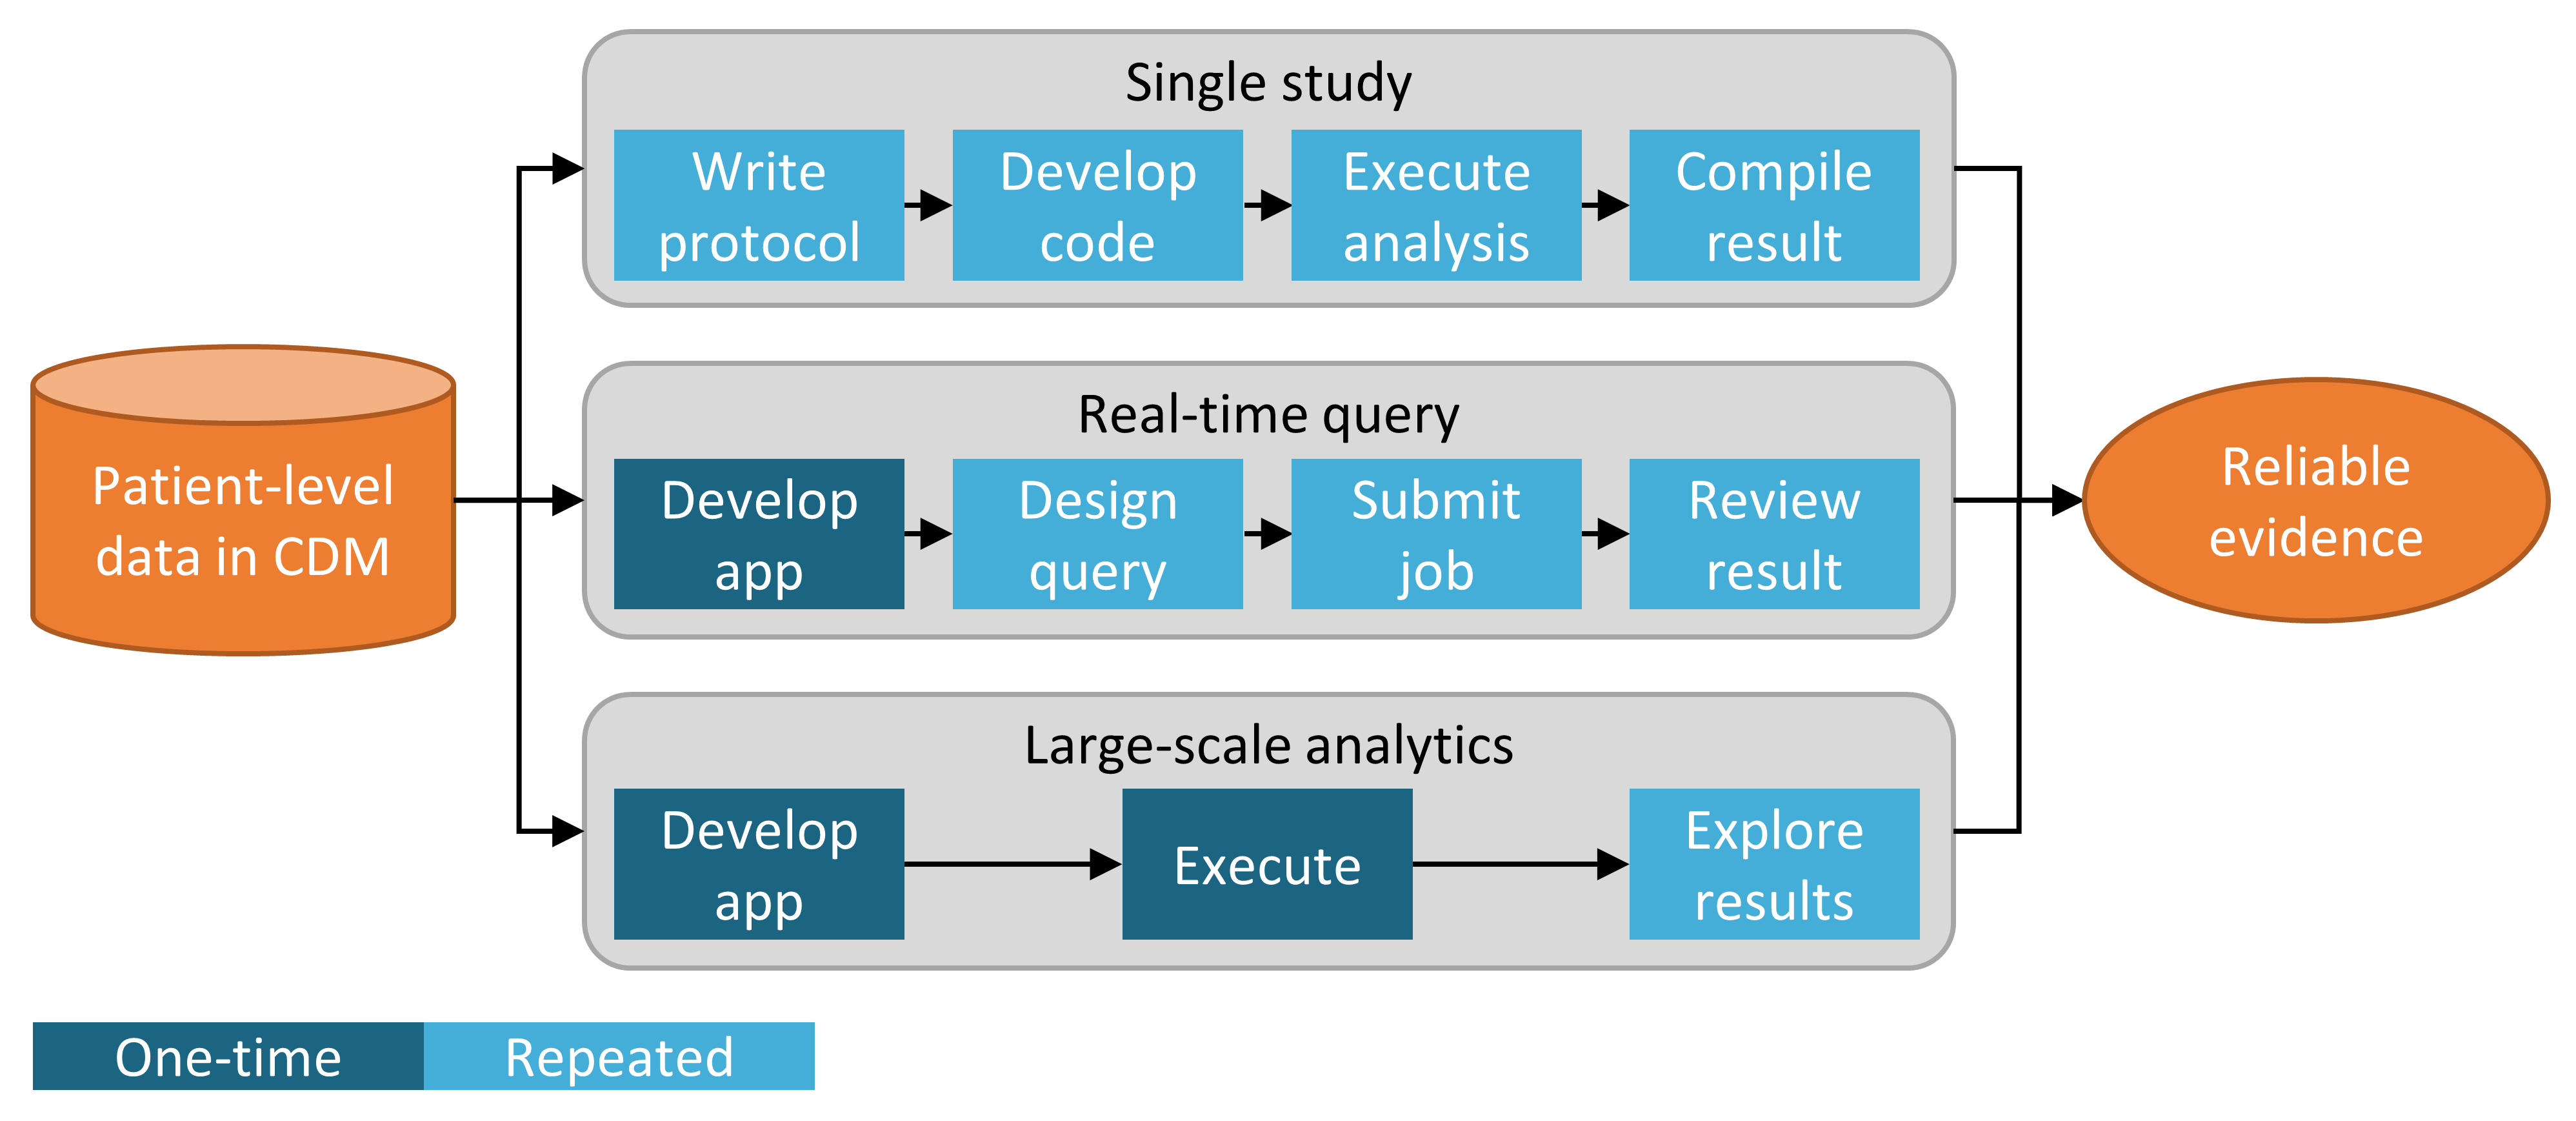
\includegraphics[width=0.9\linewidth]{images/OhdsiAnalyticsTools/strategies} 

}

\caption{(臨床の)質問に対する証拠を生成するための戦略。}\label{fig:strategies}
\end{figure}

最初の戦略では、各分析を個別の研究として扱います。分析はプロトコルで事前に指定され、コードとして実装され、データに対して実行され、その後、結果がコンパイルされ解釈されます。各質問ごとに、すべてのステップを繰り返す必要があります。そのような分析の一例は、levetiracetamとphenytoinを比較した際の血管浮腫のリスクに関するOHDSI研究です \citep[ ]{duke_2017}。 ここでは、まずプロトコルが作成され、OHDSI Methods Libraryを使用した分析コードが開発され、OHDSIネットワーク全体で実行され、結果がジャーナル公表されました。

第二の戦略では、リアルタイムまたは準リアルタイムで特定のクラスの質問に回答できるアプリケーションを開発します。アプリケーションが開発されると、ユーザーはクエリをインタラクティブに定義し、それを送信して結果を表示できます。この戦略の一例は、ATLASのコホート定義および生成ツールです。このツールは、ユーザーが様々な複雑さのコホート定義を指定し、データベースに対して定義を実行して、さまざまな包含および除外基準を満たす人数を見ることを可能にします。

第三の戦略では、同様に質問のクラスに焦点を当てますが、そのクラス内のすべての質問に対する証拠を網羅的に生成しようとします。ユーザーはその後、さまざまなインターフェースを通じて必要に応じて証拠を探索できます。一例は、うつ病治療の影響に関するOHDSI研究です \citep[ ]{schuemie_2018b}。 この研究では、すべてのうつ病治療が、4つの大規模な観察研究データベースで関心のある多数のアウトカムに対して比較されました。17,718の経験的に校正されたハザード比と広範な研究診断を含む結果の全セットは、インタラクティブなウェブアプリで利用できます。\url{http://data.ohdsi.org/SystematicEvidence/}\\

\section{ATLAS}\label{atlas}

ATLASは、CDM形式の標準化された患者レベルの観察データに対する解析の設計と実行を支援するためにOHDSIコミュニティによって開発された、無料で公開されているウェブベースのツールです。ATLASはOHDSI WebAPIと組み合わせてウェブアプリケーションとしてデプロイされ、通常はApache Tomcat上でホストされます。リアルタイム解析を行うためにはCDM内の患者レベルのデータにアクセスする必要があるため、通常は組織のファイアウォールの内側にインストールされます。しかし、パブリックATLAS\footnote{\url{http://www.ohdsi.org/web/atlas}}も存在し、このATLASインスタンスは少数の小規模なシミュレーションデータセットにしかアクセスできませんが、テストや訓練を含む多くの目的で利用可能です。パブリックインスタンスのATLASを使用して効果推定や予測研究を完全に定義し、その研究を実行するためのRコードを自動生成することも可能です。そのコードはATLASとWebAPIをインストールすることなく、利用可能なCDMが存在する任意の環境で実行できます。\index{ATLAS}

\begin{figure}

{\centering 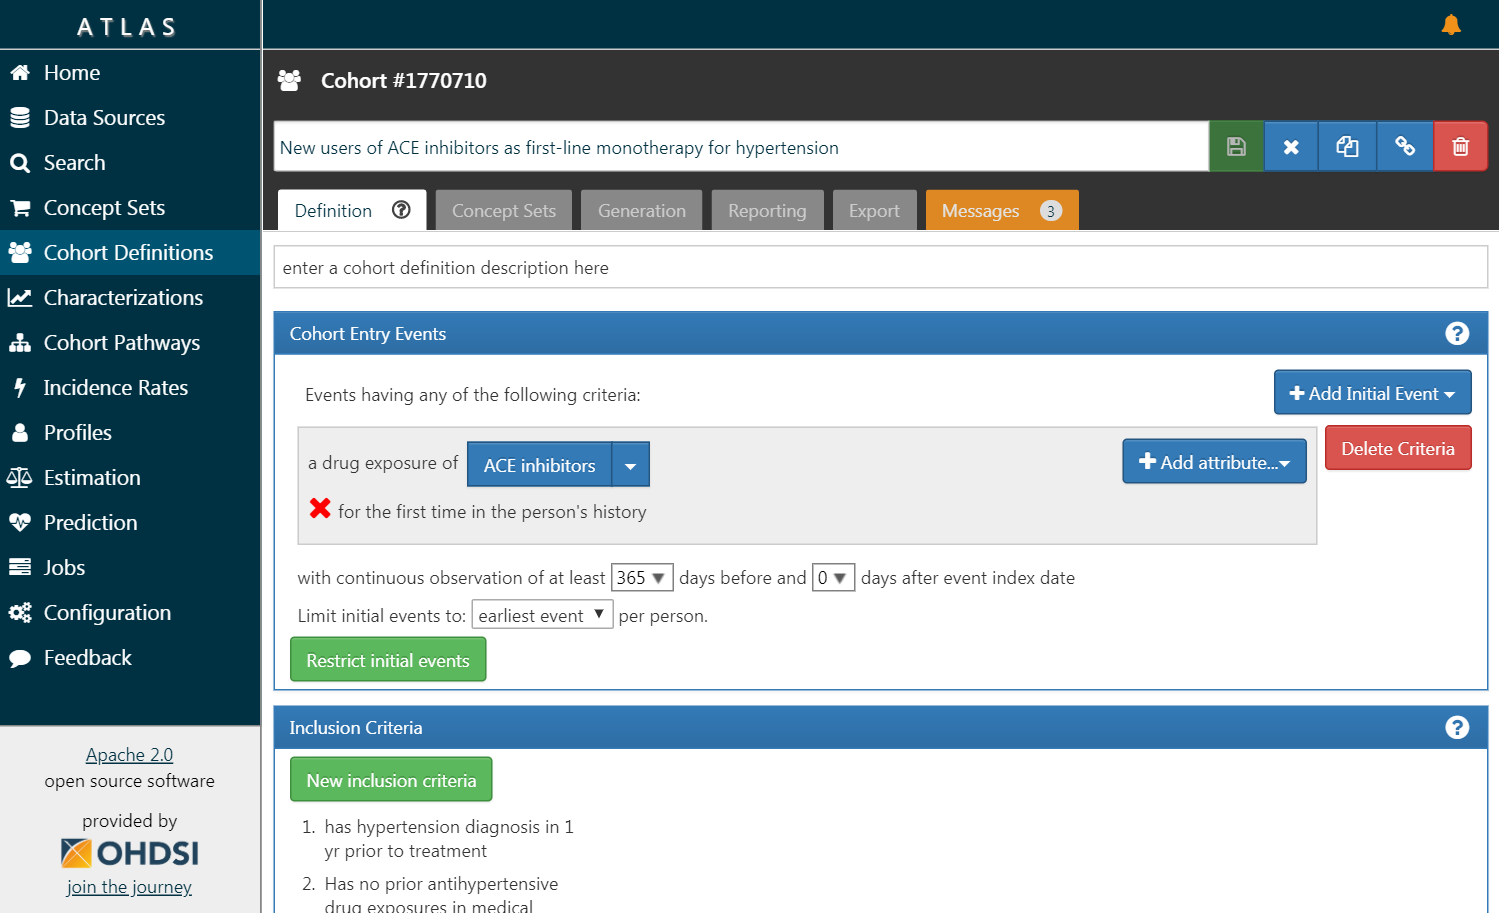
\includegraphics[width=1\linewidth]{images/OhdsiAnalyticsTools/atlas} 

}

\caption{ATLASユーザインタフェース}\label{fig:atlas}
\end{figure}

図\ref{fig:atlas}にATLASのスクリーンショットが提供されています。左側にはATLASの様々な機能を示すナビゲーションバーがあります。

\begin{description}
\item[データソース \index{ATLAS!データソース} \index{Achilles|see {ATLAS!データソース}}]
データソースは、ATLASプラットフォームに構成された各データソースの記述的、標準化されたレポートをレビューする機能を提供します。この機能は大規模分析戦略を使用し、すべての記述は事前に計算されています。データソースについては、第\ref{Characterization}章で議論されています。
\item[ボキャブラリ検索 \index{ATLAS!ボキャブラリ検索}]
ATLASはOMOP標準ボキャブラリを検索して、これらのボキャブラリにどのようなコンセプトが存在するか、そしてそのコンセプトをどう適用するかを理解するための機能を提供します。この機能については、第\ref{StandardizedVocabularies}章で議論されています。
\item[コンセプトセット \index{ATLAS!コンセプトセット}]
コンセプトセットは、標準化された分析全体で使用するコンセプトのセットを識別するために使用できる論理表現のコレクションを作成する機能を提供します。コンセプトセットは単純なコードや値のリストよりも高度な機能を提供します。コンセプトセットは、標準化されたボキャブラリからの複数のコンセプトと、関連するコンセプトの包含や除外を指定するための論理インジケータを組み合わせて構成されます。ボキャブラリの検索、コンセプトのセットの識別、そしてコンセプトセットを解決するために使用する論理の指定は、分析計画で使用されることが多い難解な医療用語を定義するための強力なメカニズムを提供します。これらのコンセプトセットはATLAS内に保存され、その後の解析の一部としてコホート定義や解析仕様に使用できます。
\item[コホート定義 \index{ATLAS!コホート定義}]
コホート定義は、一定期間内に1つ以上の基準を満たす人物のセットを構築する機能であり、これらのコホートはその後のすべての解析の入力として使用されます。この機能については、第\ref{Cohorts}章で議論されています。
\item[特性の評価\index{ATLAS!特性の評価}]
キャラクタリゼーションは、定義された1つ以上のコホートを調査し、これらの患者集団に関する特性を要約するための分析機能です。この機能はリアルタイムクエリ戦略を使用しており、第\ref{Characterization}章で議論されています。
\item[コホートパスウェイ \index{ATLAS!コホートパスウェイ}]
コホートパスウェイは、1つ以上の集団内で発生する臨床イベントのシーケンスを調査するための分析ツールです。この機能については、第\ref{Characterization}章で議論されています。
\item[発生率 \index{ATLAS!発生率}]
発生率は、対象集団内のアウトカムの発生率を推定するためのツールです。この機能については、第\ref{Characterization}章で議論されています。
\item[プロファイル \index{ATLAS!プロファイル}]
プロファイルは、個々の患者の縦断的観察データを調査し、特定の個人の状況を要約するためのツールです。この機能はリアルタイムクエリ戦略を使用します。
\item[集団レベル推定 \index{ATLAS!集団レベル推定}]
推定は、比較コホートデザインを使用して集団レベルの効果推定研究を定義するための機能であり、1つ以上のターゲットおよび比較コホート間の比較を一連の結果について調査することができます。この機能はリアルタイムクエリ戦略を実装していると言え、コーディングが不要です。第\ref{PopulationLevelEstimation}章で議論されています。
\item[患者レベル予測 \index{ATLAS!患者レベル予測}]
予測は機械学習アルゴリズムを適用して患者レベルの予測解析を行い、特定のターゲット曝露内でアウトカムを予測する機能です。この機能もリアルタイムクエリ戦略を実装しており、コーディングが不要です。第\ref{PatientLevelPrediction}章で議論されています。
\item[ジョブ \index{ATLAS!ジョブ}]
ジョブメニュー項目を選択して、WebAPIを通じて実行されているプロセスの状態を調査します。ジョブは、コホートの生成やコホートの特性評価レポートの計算など、長時間実行されるプロセスです。
\item[設定 \index{ATLAS!設定}]
構成メニュー項目を選択して、ソース構成セクションに構成されたデータソースを確認します。
\item[フィードバック \index{ATLAS!フィードバック}]
フィードバックリンクをクリックすると、ATLASの問題ログにアクセスできます。新しい問題のログを記録したり、既存の問題を検索したりできます。新しい機能や改善のアイデアがある場合も、開発コミュニティのためにこの場所で記載できます。
\end{description}

\subsection{セキュリティ}\label{ux30bbux30adux30e5ux30eaux30c6ux30a3}

ATLASとWebAPIは、プラットフォーム全体で機能やデータソースへのアクセスを制御するための細かいセキュリティモデルを提供します。セキュリティシステムはApache Shiroライブラリを活用して構築されています。セキュリティシステムの詳細は、オンラインのWebAPIセキュリティwikiで確認できます。\footnote{\url{https://github.com/OHDSI/WebAPI/wiki/Security-Configuration}} \index{ATLAS!セキュリティ}

\subsection{ドキュメント}\label{ux30c9ux30adux30e5ux30e1ux30f3ux30c8}

ATLASのドキュメントは、ATLAS GitHubリポジトリのwikiでオンラインで確認できます。\footnote{\url{https://github.com/OHDSI/ATLAS/wiki}} このwikiには、様々なアプリケーション機能に関する情報や、オンラインビデオチュートリアルへのリンクが含まれています。 \index{ATLAS!ドキュメント}

\subsection{インストール方法}\label{ux30a4ux30f3ux30b9ux30c8ux30fcux30ebux65b9ux6cd5}

ATLASのインストールは、OHDSI WebAPIと組み合わせて行われます。各コンポーネントのインストールガイドは、ATLAS GitHubリポジトリのセットアップガイド\footnote{\url{https://github.com/OHDSI/Atlas/wiki/Atlas-Setup-Guide}}およびWebAPI GitHubリポジトリのインストールガイドにオンラインで提供されています。 \index{ATLAS!インストール}

\section{メソッドライブラリ}\label{ux30e1ux30bdux30c3ux30c9ux30e9ux30a4ux30d6ux30e9ux30ea}

\href{https://ohdsi.github.io/MethodsLibrary/}{OHDSIメソッドライブラリ}は、図 \ref{fig:methodsLibrary} に示されているオープンソースのRパッケージのコレクションです。 \index{methods library}

\begin{figure}

{\centering 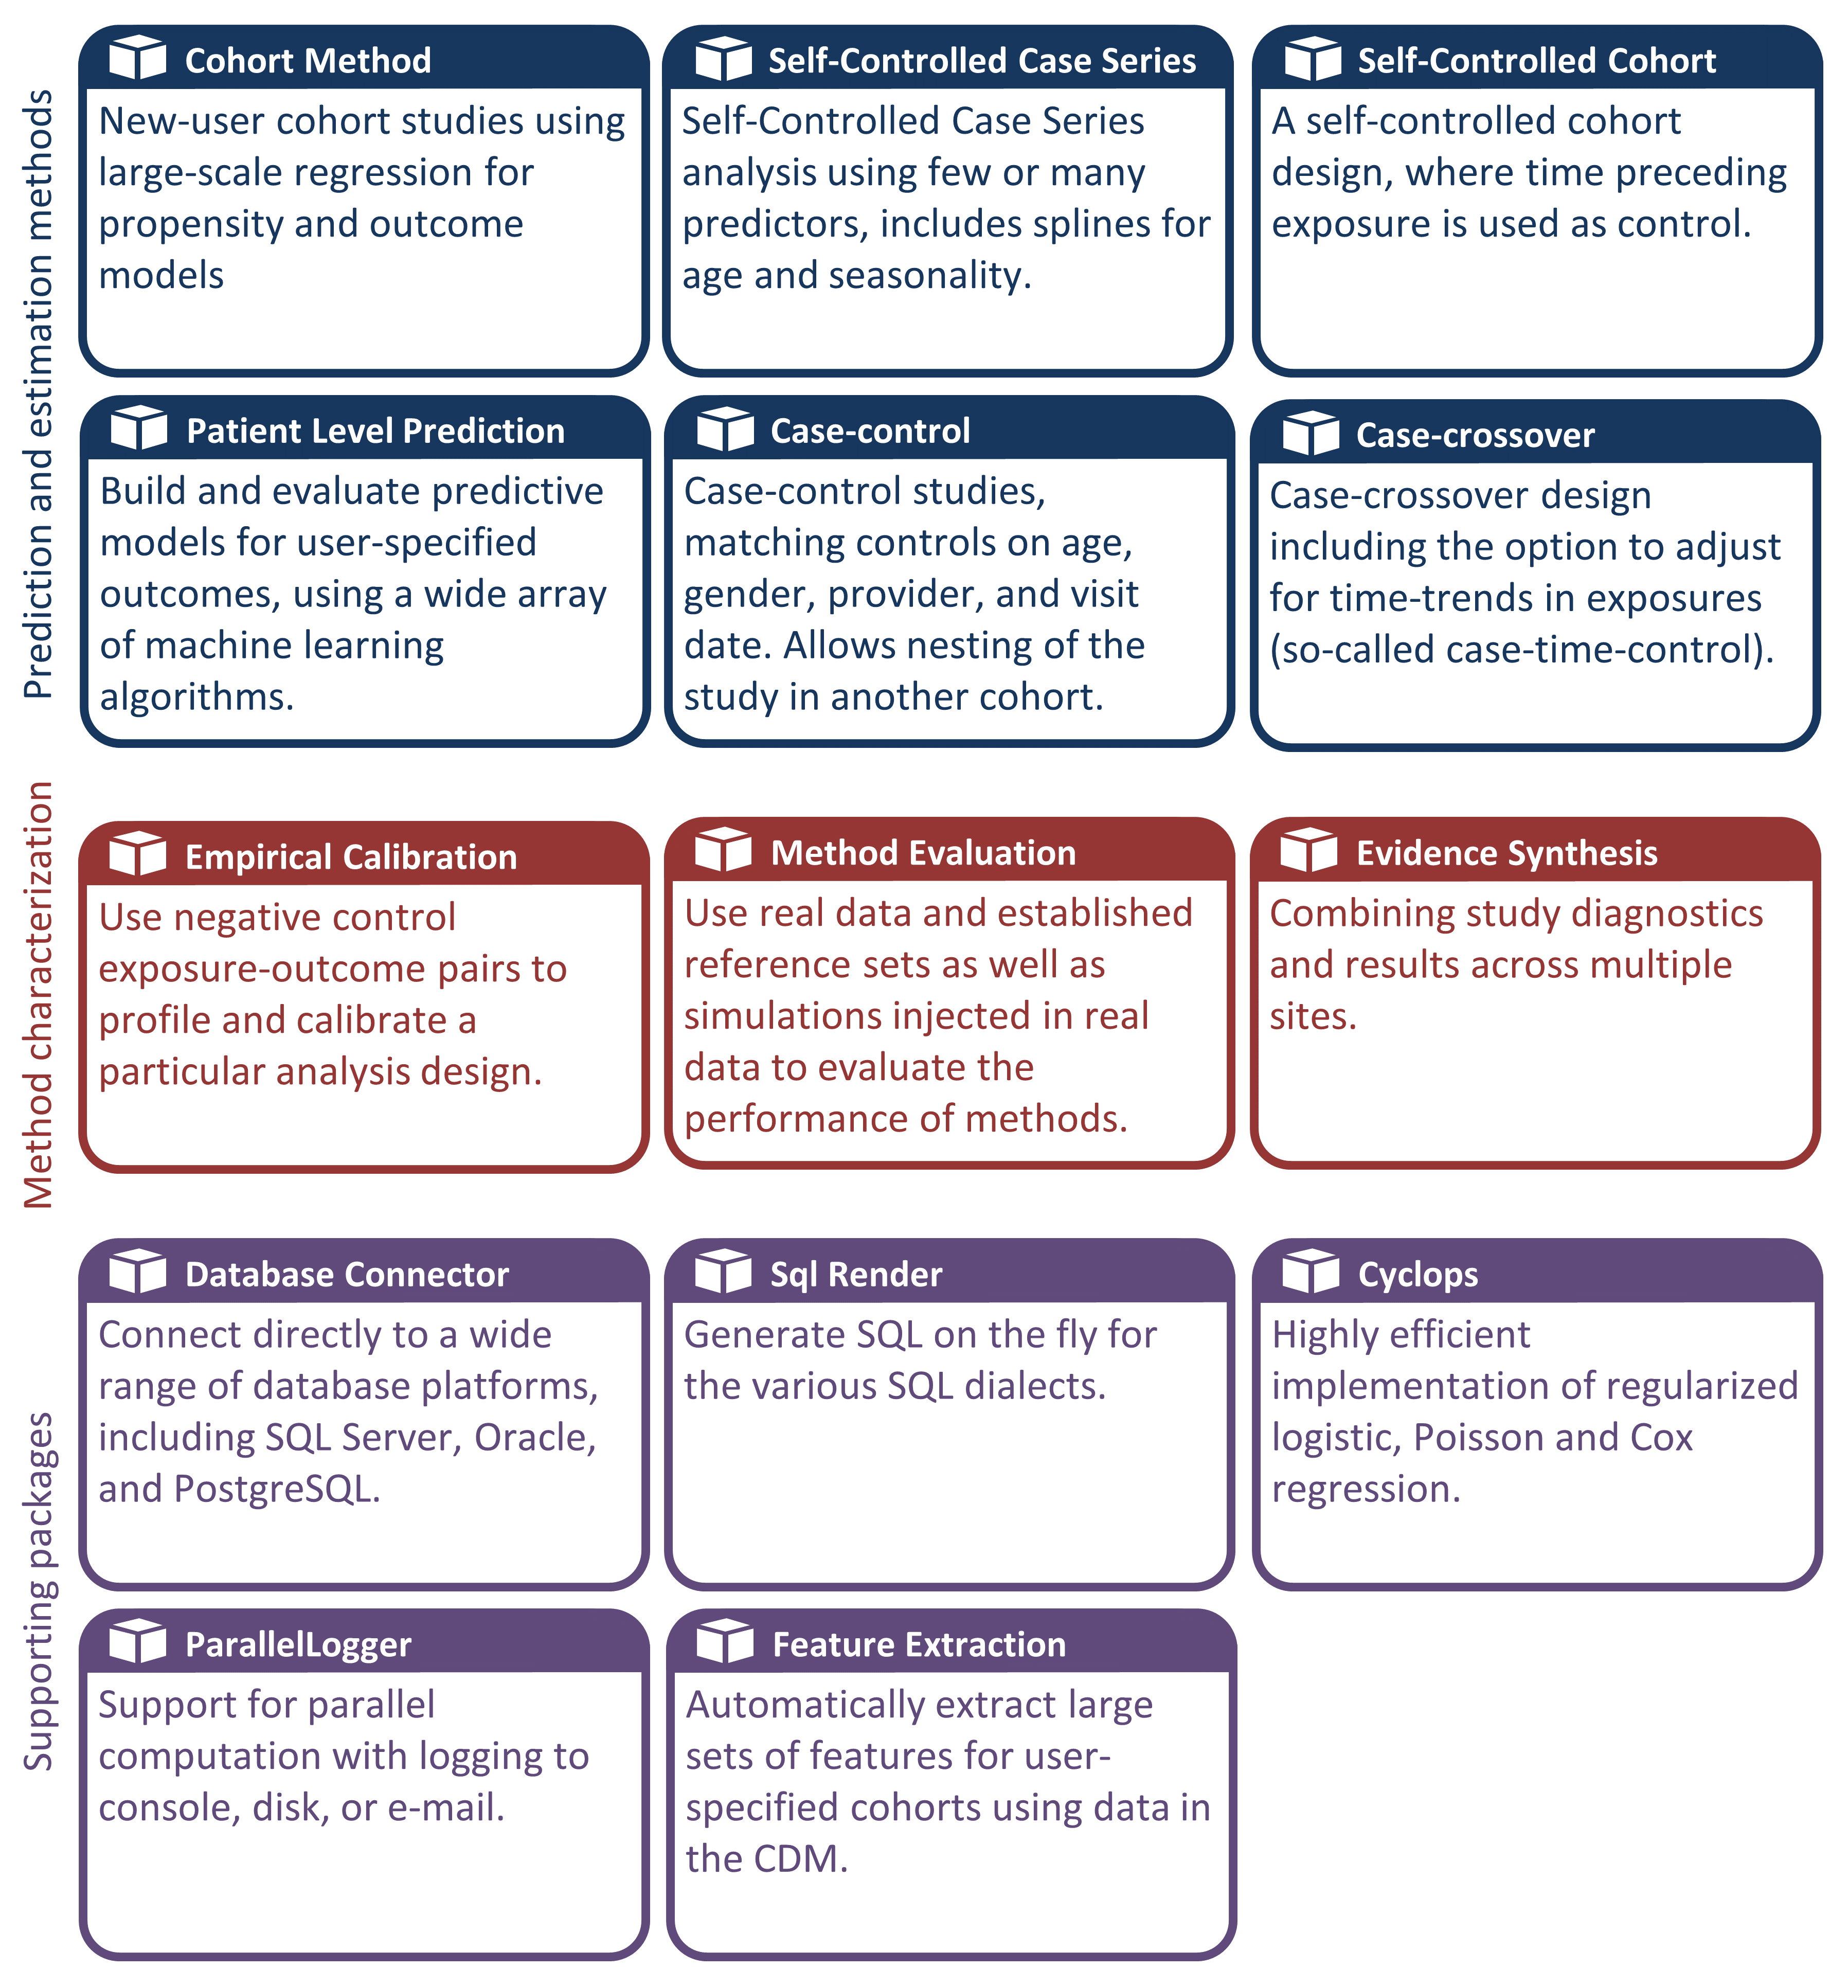
\includegraphics[width=1\linewidth]{images/OhdsiAnalyticsTools/methodsLibrary} 

}

\caption{OHDSIメソッドライブラリのパッケージ。}\label{fig:methodsLibrary}
\end{figure}

これらのパッケージは、CDM内のデータから始まり、推定値や支援統計、図表を生成する完全な観察研究を実施するためのR関数を提供します。これらのパッケージはCDM内の観察データと直接対話し、カスタム分析を可能にし、あるいは標準化された高度な分析機能を提供することができます(詳細はChapter \ref{SqlAndR}、Chapter \ref{Characterization}、Chapter \ref{PopulationLevelEstimation}、Chapter \ref{PatientLevelPrediction}を参照してください)。メソッドライブラリは、透明性、再現性、異なるコンテキストでのメソッドの操作特性の測定、およびメソッドによって生成される推定値の経験的校正など、過去および現在の研究から学んだベストプラクティスをサポートしています。

メソッドライブラリは多くの公表された臨床研究 \citetext{\citealp[ ]{boland_2017}; \citealp[ ]{duke_2017}; \citealp[ ]{ramcharran_2017}; \citealp[ ]{weinstein_2017}; \citealp[ ]{wang_2017}; \citealp[ ]{ryan_2017}; \citealp[ ]{ryan_2018}; \citealp[ ]{vashisht_2018}; \citealp[ ]{yuan_2018}; \citealp[ ]{johnston_2019}} で使われており、方法論の研究にも利用されています \citetext{\citealp[ ]{schuemie_2014}; \citealp[ ]{schuemie_2016}; \citealp[ ]{reps2018}; \citealp[ ]{tian_2018}; \citealp[ ]{schuemie_2018}; \citealp[ ]{schuemie_2018b}; \citealp[ ]{reps_2019}}。メソッドライブラリにおけるメソッドの実装の妥当性についてはChapter \ref{SoftwareValidity}で説明されています。

\subsection{大規模分析サポート}\label{ux5927ux898fux6a21ux5206ux6790ux30b5ux30ddux30fcux30c8}

すべてのパッケージで組み込まれている主な機能の一つは、多くの分析を効率的に実行できることです。例えば、集団レベルの推定を行う場合、CohortMethodパッケージは多くの暴露とアウトカムに対して効果サイズの推定を行うことを可能にし、様々な分析設定を使用して、必要な中間データセットおよび最終データセットを計算するための最適な方法を自動的に選択します。共変量の抽出や、一つのターゲット・コンパレータペアに対して複数のアウトカムに使用される傾向スコアモデルの適合など、使い回しが可能なステップは一度だけ実行されます。可能な場合は、計算リソースを最大限に活用するために計算は並行して行われます。

この計算効率は一度に多くの質問に答える大規模分析を可能にし、我々のメソッドの操作特性を測定し、Chapter \ref{MethodValidity}で説明されているように推定値の経験的校正を行うために必要な対照仮説(例:陰性対照)を含むことが重要です。 \index{control hypotheses}

\subsection{ビッグデータ対応}\label{BigDataSupport}

メソッドライブラリは、非常に大きなデータベースに対しても計算を行うことができるように設計されています。これは次の三つの方法で達成されます:

\begin{enumerate}
\def\labelenumi{\arabic{enumi}.}
\tightlist
\item
  大部分のデータ操作はデータベースサーバーで行われます。分析は通常、データベース内の全データのごく一部しか必要としないため、メソッドライブラリはSqlRenderおよびDatabaseConnectorパッケージを介してサーバー上で高度な操作を行い、関連データを前処理および抽出することができます。
\item
  大量のローカルデータオブジェクトはメモリ効率の良い方法で保存されます。ローカルマシンにダウンロードされるデータについては、メソッドライブラリは\href{https://cran.r-project.org/web/packages/ff}{ff}パッケージを使用して大規模データオブジェクトを保存および操作します。これにより、メモリに収まらない大きなデータと作業することが可能です。
\item
  必要に応じて高性能コンピューティングが適用されます。例えば、\href{https://ohdsi.github.io/Cyclops/}{Cyclops}パッケージは、メソッドライブラリ全体で使用される高効率な回帰エンジンを実装しており、これにより通常は適合できない大規模な回帰(多くの変数、大量の観測値)を実行することができます。
\end{enumerate}

\subsection{ドキュメント}\label{ux30c9ux30adux30e5ux30e1ux30f3ux30c8-1}

Rはパッケージを文書化するための標準的な方法を提供します。各パッケージには、パッケージに含まれるすべての関数およびデータセットを文書化した\emph{パッケージマニュアル}があります。すべてのパッケージマニュアルは、Methods Libraryのウェブサイト\footnote{\url{https://ohdsi.github.io/MethodsLibrary}}、パッケージのGitHubリポジトリ、CRANで利用できます。さらに、R内からパッケージマニュアルを参照することができ、例えばDatabaseConnectorパッケージを読み込んだ後、コマンド\texttt{?connect}を入力すると「connect」関数に関するドキュメントが表示されます。

パッケージマニュアルに加えて、多くのパッケージは\emph{ビネット}も提供しています。ビネットは、特定のタスクを実行するためにパッケージをどのように使用するかを説明した長文のドキュメントです。例えば、一つのビネット\footnote{\url{https://ohdsi.github.io/CohortMethod/articles/MultipleAnalyses.html}}では、CohortMethodパッケージを使用して複数の分析を効率的に実行する方法を説明しています。ビネットはMethods Libraryのウェブサイト、パッケージのGitHubリポジトリ、およびCRANでも見つけることができます。 \index{vignette}

\subsection{システム要件}\label{ux30b7ux30b9ux30c6ux30e0ux8981ux4ef6}

システム要件を検討する際に関連する二つのコンピューティング環境があります:データベースサーバーと分析ワークステーションです。 \index{system requirements}

データベースサーバーはCDM形式の観察医療データを保持する必要があります。メソッドライブラリは、従来のデータベースシステム(PostgreSQL、Microsoft SQL Server、Oracle)、パラレルデータウェアハウス(Microsoft APS、IBM Netezza、Amazon Redshift)、およびビッグデータプラットフォーム(Impala経由でのHadoop、Google BigQuery)を含む幅広いデータベース管理システムをサポートしています。

分析ワークステーションは、メソッドライブラリがインストールされ実行される場所です。これがローカルマシン(例えば、ノートパソコン)か、RStudio Serverが実行されるリモートサーバーかに関わらず、Rがインストールされている必要があります。可能であればRStudioも一緒にインストールすることをお勧めします。また、Methods LibraryはJavaがインストールされている必要があります。分析ワークステーションはデータベースサーバーに接続できる必要があり、具体的にはファイアウォールがその間のアクセスポートを開いている必要があります。一部の分析は計算集中的であるため、複数のプロเซッサコアと十分なメモリを持つことが分析の高速化につながります。少なくとも4つのコアと16ギガバイトのメモリを推奨します。

\subsection{インストール方法}\label{installR}

OHDSI Rパッケージを実行するために必要な環境をインストールするための手順は次の通りです。インストールする必要があるものは4つあります: \index{R!installation}

\begin{enumerate}
\def\labelenumi{\arabic{enumi}.}
\tightlist
\item
  \textbf{R}は統計的コンピューティング環境です。基本的なユーザインターフェースとして主にコマンドラインインターフェースを提供します。
\item
  \textbf{Rtools}は、WindowsでRパッケージをソースからビルドするために必要なプログラム群です。
\item
  \textbf{RStudio}は、Rを使いやすくするIDE(統合開発環境)です。コードエディタ、デバッグ、およびビジュアルツールが含まれています。よろしくお願いいたします。
\end{enumerate}

\section{展開戦略}\label{ux5c55ux958bux6226ux7565}

ATLASやMethods Libraryを含む全体のOHDSIツールスタックを組織内で展開することは、非常に困難な作業です。依存関係がある多くのコンポーネントを考慮し、設定を行う必要があります。このため、二つの取り組みが、すべてのスタックを一つのパッケージとしてインストールできる統合展開戦略を開発しました。一部の仮想化技術を使用して、これを実現します。それが、BroadseaおよびAmazon Web Services (AWS)です。 \index{tools deployment}

\subsection{Broadsea}\label{broadsea}

Broadsea\footnote{\url{https://github.com/OHDSI/Broadsea}}はDockerコンテナ技術を使用します。{[}\^{}\^{}dockerUrl{]} OHDSIツールは依存関係とともに、Dockerイメージと呼ばれる単一のポータブルなバイナリファイルにパッケージ化されています。このイメージはDockerエンジンサービス上で実行され、すべてのソフトウェアがインストールされてすぐに実行可能な仮想マシンが作成されます。DockerエンジンはMicrosoft Windows、MacOS、Linuxなどのほとんどのオペレーティングシステムで利用可能です。Broadsea Dockerイメージには、Methods LibraryやATLASを含む主要なOHDSIツールが含まれています。 \index{tools deployment!Broadsea}

\subsection{Amazon AWS}\label{amazon-aws}

Amazonは、AWSクラウドコンピューティング環境でボタンをクリックするだけでインスタンス化できる二つの環境を用意しています:OHDSI-in-a-Box\footnote{\url{https://github.com/OHDSI/OHDSI-in-a-Box}}とOHDSIonAWSです。{[}\^{}\^{}ohdsiOnAwsUrl{]} \index{tools deployment!Amazon AWS}

OHDSI-in-a-Boxは学習環境として特に作成されており、OHDSIコミュニティによって提供されるほとんどのチュートリアルで使用されます。これには多くのOHDSIツール、サンプルデータセット、RStudioおよび他の補助ソフトウェアが一つの低コストのWindows仮想マシンに含まれています。CDMを保存するためにPostgreSQLデータベースが使用され、ATLASの中間結果も格納されます。OMOP CDMデータマッピングおよびETLツールもOHDSI-in-a-Boxに含まれています。OHDSI-in-a-Boxのアーキテクチャは図\ref{fig:ohdsiinaboxDiagram}に示されています。

\begin{figure}

{\centering 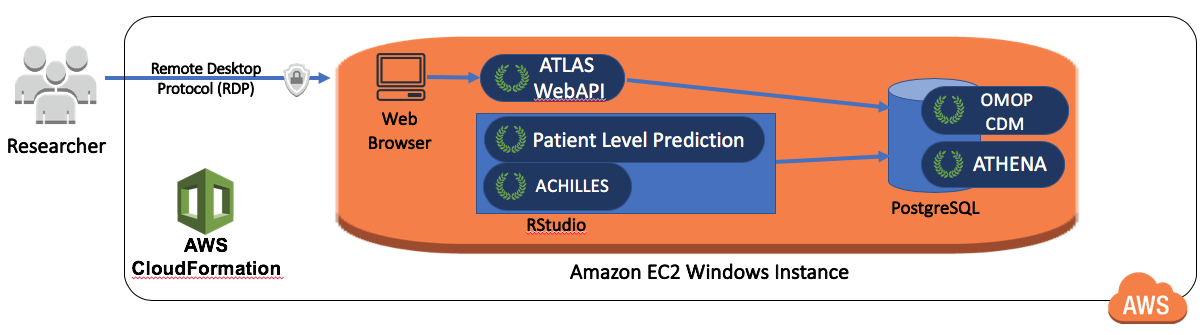
\includegraphics[width=1\linewidth]{images/OhdsiAnalyticsTools/OHDSI-in-a-BoxDiagram} 

}

\caption{OHDSI-in-a-BoxのAmazon Web Servicesアーキテクチャ。}\label{fig:ohdsiinaboxDiagram}
\end{figure}

OHDSIonAWSは、エンタープライズクラスの複数ユーザー対応、スケーラブルでフォールトトレラントなOHDSI環境のリファレンスアーキテクチャで、組織がデータ分析を行うために使用できます。いくつかのサンプルデータセットが含まれており、組織の実際の医療データを自動的に読み込むこともできます。データはAmazon Redshiftデータベースプラットフォームに配置され、これをOHDSIツールがサポートします。ATLASの中間結果はPostgreSQLデータベースに格納されます。フロントエンドでは、ユーザーはウェブインターフェースを通じてATLASおよびRStudioにアクセスできます(RStudio Serverを活用)。RStudioではOHDSI Methods Libraryがすでにインストールされており、データベースに接続して使用することができます。OHDSIonAWSの展開の自動化はオープンソースであり、組織の管理ツールとベストプラクティスを含むようにカスタマイズできます。OHDSIonAWSのアーキテクチャは図\ref{fig:ohdsionawsDiagram}に示されています。

\begin{figure}

{\centering 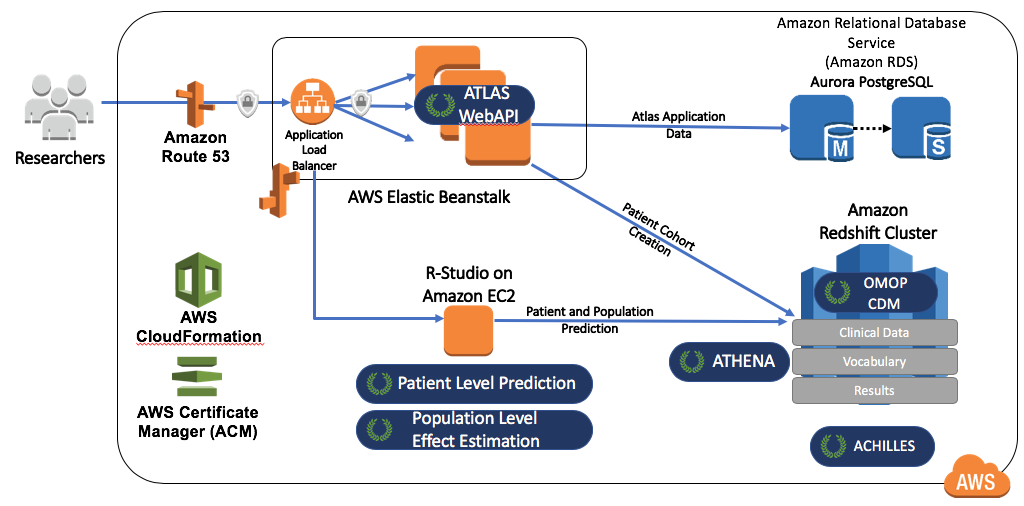
\includegraphics[width=1\linewidth]{images/OhdsiAnalyticsTools/OHDSIonAWSDiagram} 

}

\caption{OHDSIonAWSのAmazon Web Servicesアーキテクチャ。}\label{fig:ohdsionawsDiagram}
\end{figure}

\section{まとめ}\label{ux307eux3068ux3081-6}

\begin{rmdsummary}
\begin{itemize}
\tightlist
\item
  CDM内のデータに対して分析を行うには

  \begin{itemize}
  \tightlist
  \item
    カスタムコードの作成
  \item
    OHDSI Methods LibraryのRパッケージを使用したコードの作成
  \item
    インタラクティブ分析プラットフォームATLASの使用
  \end{itemize}
\item
  OHDSIツールは異なる分析戦略を使用します

  \begin{itemize}
  \tightlist
  \item
    単一研究
  \item
    リアルタイムクエリ
  \item
    大規模アナリティクス
  \end{itemize}
\item
  ほとんどのOHDSIアナリティクスツールは以下に埋め込まれています

  \begin{itemize}
  \tightlist
  \item
    インタラクティブ分析プラットフォームATLAS
  \item
    OHDSI Methods LibraryのRパッケージ
  \end{itemize}
\item
  OHDSIツールの展開を容易にするいくつかの戦略があります。
\end{itemize}
\end{rmdsummary}

\chapter{第9章 --翻訳作業中-- SQLとR}\label{SqlAndR}

\emph{チャプタリーダー: Martijn Schuemie \& Peter Rijnbeek}

共通データモデル(CDM)はリレーショナルデータベースモデルです(すべてのデータはフィールドを持つテーブルのレコードとして表されます)。そのため、データは通常、PostgreSQL、Oracle、またはMicrosoft SQL Serverなどのソフトウェアプラットフォームを使用してリレーショナルデータベースに保存されます。ATLASやMethods LibraryなどのさまざまなOHDSIツールは、バックグラウンドでデータベースをクエリすることによって機能しますが、適切なアクセス権を持っていれば、私たちも直接データベースにクエリを実行することができます。これを行う主な理由は、現在のツールではサポートされていない分析を実行するためです。しかし、直接のクエリはミスを犯すリスクが高まり、OHDSIツールはしばしば適切なデータ分析へのガイドとして設計されているため、直接クエリにはそのようなガイドが提供されません。

リレーショナルデータベースをクエリする標準的な言語はSQL(Structured Query Language)で、クエリやデータ変更に使用できます。SQLの基本コマンドは確かに標準化されており、すべてのソフトウェアプラットフォームで同じですが、各プラットフォームには独自の表現があり、微妙な変更があります。例えば、SQL ServerでPERSONテーブルの上位10行を取得するには、次のように入力します: \index{SQL} \index{structured query language|see {SQL}}

\begin{Shaded}
\begin{Highlighting}[]
\KeywordTok{SELECT}\NormalTok{ TOP }\DecValTok{10} \OperatorTok{*} \KeywordTok{FROM}\NormalTok{ person;}
\end{Highlighting}
\end{Shaded}

一方、PostgreSQLでは同じクエリは次のようになります:

\begin{Shaded}
\begin{Highlighting}[]
\KeywordTok{SELECT} \OperatorTok{*} \KeywordTok{FROM}\NormalTok{ person }\KeywordTok{LIMIT} \DecValTok{10}\NormalTok{;}
\end{Highlighting}
\end{Shaded}

OHDSIでは、プラットフォーム固有の表現に依存しないことを望んでいます。すなわち、すべてのOHDSIデータベースで同じSQL言語を使用したいと考えています。このため、OHDSIは\href{https://ohdsi.github.io/SqlRender/}{SqlRender}パッケージを開発しました。これは、ある標準表現から後述するサポートされる表現のいずれかに翻訳できるRパッケージです。この標準表現 - \textbf{OHDSI SQL} - は主にSQL Server SQL表現のサブセットです。今章の例示するSQL文はすべてOHDSI SQLを使用します。 \index{SqlRender} \index{agnostic SQL|see {SqlRender}} \index{Standard SQL Dialect|see {SqlRender}} \index{OHDSI SQL|see {SqlRender}}

各データベースプラットフォームには、SQLを使用したデータベースのクエリのための独自のソフトウェアツールも付属しています。OHDSIでは、多くのデータベースプラットフォームに接続できる1つのRパッケージである\href{https://ohdsi.github.io/DatabaseConnector/}{DatabaseConnector}パッケージを開発しました。DatabaseConnectorも今章後半で説明します。 \index{DatabaseConnector}

したがって、CDMに準拠したデータベースに対してOHDSIツールを使用せずにクエリを実行できますが、推奨されるパスはDatabaseConnectorとSqlRenderパッケージを使用することです。これにより、1つのサイトで開発されたクエリが他のサイトでも修正なしで使用できるようになります。さらに、R自体がデータベースから抽出されたデータをさらに分析するための機能(統計分析の実行や(インタラクティブな)プロットの生成)を即座に提供します。 \index{R}

この章では、読者がSQLの基本的な理解を持っていることを前提としています。まず、SqlRenderとDatabaseConnectorの使用方法をレビューします。これらのパッケージを使用しない場合は、これらのセクションをスキップできます。セクション\ref{QueryTheCdm}では、CDMをクエリするためのSQL(この場合OHDSI SQL)使用方法を説明します。次のセクションでは、CDMをクエリする際にOHDSI標準化ボキャブラリを使用する方法を強調します。CDMに対する一般的なクエリのコレクションであるQueryLibraryを紹介し、公開されています。最後に、発現率を推定する例の研究を示し、この研究をSqlRenderとDatabaseConnectorを使用して実装します。 \index{Query Library} \index{SQL Query Library|see {Query Library}}

\section{SqlRender}\label{SqlRender}

\href{https://ohdsi.github.io/SqlRender/}{SqlRender} パッケージは CRAN(Comprehensive R Archive Network)で利用可能であり、以下の方法でインストールできます:

\begin{Shaded}
\begin{Highlighting}[]
\FunctionTok{install.packages}\NormalTok{(}\StringTok{"SqlRender"}\NormalTok{)}
\end{Highlighting}
\end{Shaded}

SqlRenderは、従来のデータベースシステム(PostgreSQL、Microsoft SQL Server、SQLite、Oracle)を含む幅広い技術プラットフォーム、並列データウェアハウス(Microsoft APS、IBM Netezza、Amazon Redshift)、およびビッグデータプラットフォーム(Impala経由のHadoop、Google BigQuery)をサポートしています。このRパッケージには、パッケージマニュアルと機能の全体を探るためのビネットが付属しています。ここでは、主な機能のいくつかを説明します。

\subsection{SQLのパラメータ設定}\label{sqlux306eux30d1ux30e9ux30e1ux30fcux30bfux8a2dux5b9a}

パッケージの機能の一つは、SQLのパラメータ設定をサポートすることです。しばしば、いくつかのパラメータに基づいて小さなバリエーションのSQLを生成する必要があります。SqlRenderは、SQLコード内にパラメータ設定を可能にするシンプルなマークアップ文法を提供します。パラメータ値に基づいてSQLをレンダリングするには、\texttt{render()}関数を使用します。 \index{SqlRender!parameterization}

\subsubsection*{パラメータ値の置換}\label{ux30d1ux30e9ux30e1ux30fcux30bfux5024ux306eux7f6eux63db}
\addcontentsline{toc}{subsubsection}{パラメータ値の置換}

\texttt{@} 文字を使用して、レンダリング時に実際のパラメータ値と交換する必要があるパラメータ名を示します。以下の例では、SQL内で \texttt{a} という変数が言及されています。\texttt{render} 関数の呼び出しでは、このパラメータの値が定義されています:

\begin{Shaded}
\begin{Highlighting}[]
\NormalTok{sql }\OtherTok{\textless{}{-}} \StringTok{"SELECT * FROM concept WHERE concept\_id = @a;"}
\FunctionTok{render}\NormalTok{(sql, }\AttributeTok{a =} \DecValTok{123}\NormalTok{)}
\end{Highlighting}
\end{Shaded}

\begin{verbatim}
## [1] "SELECT * FROM concept WHERE concept_id = 123;"
\end{verbatim}

ほとんどのデータベース管理システムが提供するパラメータ設定とは異なり、値だけでなくテーブルやフィールド名も簡単にパラメータ化できます:

\begin{Shaded}
\begin{Highlighting}[]
\NormalTok{sql }\OtherTok{\textless{}{-}} \StringTok{"SELECT * FROM @x WHERE person\_id = @a;"}
\FunctionTok{render}\NormalTok{(sql, }\AttributeTok{x =} \StringTok{"observation"}\NormalTok{, }\AttributeTok{a =} \DecValTok{123}\NormalTok{)}
\end{Highlighting}
\end{Shaded}

\begin{verbatim}
## [1] "SELECT * FROM observation WHERE person_id = 123;"
\end{verbatim}

パラメータ値は、数値、文字列、ブール値、ベクターであり、コンマ区切りリストに変換されます:

\begin{Shaded}
\begin{Highlighting}[]
\NormalTok{sql }\OtherTok{\textless{}{-}} \StringTok{"SELECT * FROM concept WHERE concept\_id IN (@a);"}
\FunctionTok{render}\NormalTok{(sql, }\AttributeTok{a =} \FunctionTok{c}\NormalTok{(}\DecValTok{123}\NormalTok{, }\DecValTok{234}\NormalTok{, }\DecValTok{345}\NormalTok{))}
\end{Highlighting}
\end{Shaded}

\begin{verbatim}
## [1] "SELECT * FROM concept WHERE concept_id IN (123,234,345);"
\end{verbatim}

\subsubsection*{If-Then-Else}\label{if-then-else}
\addcontentsline{toc}{subsubsection}{If-Then-Else}

時々、あるパラメータの値に基づいてコードのブロックをオンまたはオフにする必要があります。これは \texttt{\{Condition\}\ ?\ \{if\ true\}\ :\ \{if\ false\}} 構文を使用して行われます。\emph{condition} が true または 1 の場合、\emph{if true} ブロックが使用され、それ以外の場合は \emph{if false} ブロックが表示されます(存在する場合)。

\begin{Shaded}
\begin{Highlighting}[]
\NormalTok{sql }\OtherTok{\textless{}{-}} \StringTok{"SELECT * FROM cohort \{@x\} ? \{WHERE subject\_id = 1\}"}
\FunctionTok{render}\NormalTok{(sql, }\AttributeTok{x =} \ConstantTok{FALSE}\NormalTok{)}
\end{Highlighting}
\end{Shaded}

\begin{verbatim}
## [1] "SELECT * FROM cohort "
\end{verbatim}

\begin{Shaded}
\begin{Highlighting}[]
\FunctionTok{render}\NormalTok{(sql, }\AttributeTok{x =} \ConstantTok{TRUE}\NormalTok{)}
\end{Highlighting}
\end{Shaded}

\begin{verbatim}
## [1] "SELECT * FROM cohort WHERE subject_id = 1"
\end{verbatim}

簡単な比較もサポートされています:

\begin{Shaded}
\begin{Highlighting}[]
\NormalTok{sql }\OtherTok{\textless{}{-}} \StringTok{"SELECT * FROM cohort \{@x == 1\} ? \{WHERE subject\_id = 1\};"}
\FunctionTok{render}\NormalTok{(sql, }\AttributeTok{x =} \DecValTok{1}\NormalTok{)}
\end{Highlighting}
\end{Shaded}

\begin{verbatim}
## [1] "SELECT * FROM cohort WHERE subject_id = 1;"
\end{verbatim}

\begin{Shaded}
\begin{Highlighting}[]
\FunctionTok{render}\NormalTok{(sql, }\AttributeTok{x =} \DecValTok{2}\NormalTok{)}
\end{Highlighting}
\end{Shaded}

\begin{verbatim}
## [1] "SELECT * FROM cohort ;"
\end{verbatim}

\texttt{IN} 演算子もサポートされています:

\begin{Shaded}
\begin{Highlighting}[]
\NormalTok{sql }\OtherTok{\textless{}{-}} \StringTok{"SELECT * FROM cohort \{@x IN (1,2,3)\} ? \{WHERE subject\_id = 1\};"}
\FunctionTok{render}\NormalTok{(sql, }\AttributeTok{x =} \DecValTok{2}\NormalTok{)}
\end{Highlighting}
\end{Shaded}

\begin{verbatim}
## [1] "SELECT * FROM cohort WHERE subject_id = 1;"
\end{verbatim}

\subsection{他のSQL表現への置換}\label{ux4ed6ux306esqlux8868ux73feux3078ux306eux7f6eux63db}

\href{https://ohdsi.github.io/SqlRender/}{SqlRender} パッケージのもう一つの機能は、OHDSI SQLから他のSQL表現へ翻訳することです。例えば:

\begin{Shaded}
\begin{Highlighting}[]
\NormalTok{sql }\OtherTok{\textless{}{-}} \StringTok{"SELECT TOP 10 * FROM person;"}
\FunctionTok{translate}\NormalTok{(sql, }\AttributeTok{targetDialect =} \StringTok{"postgresql"}\NormalTok{)}
\end{Highlighting}
\end{Shaded}

\begin{verbatim}
## [1] "SELECT  * FROM person LIMIT 10;"
## attr(,"sqlDialect")
## [1] "postgresql"
\end{verbatim}

\texttt{targetDialect} パラメータには次の値が設定可能です:``oracle'', ``postgresql'', ``pdw'', ``redshift'', ``impala'', ``netezza'', ``bigquery'', ``sqlite'', ``sql server''。 \index{SqlRender!translation}

\begin{rmdimportant}
すべてのSQL関数や構造を正確に翻訳するには限界があります。パッケージに実装されている翻訳ルールが限られているためでもあり、一部のSQL機能がすべての表現に同等のものを持たないためです。これは、OHDSI SQLが独自の新しいSQL表現として開発された主な理由です。それでも、可能な限り、車輪の再発明を避けるためにSQL Serverの構文を維持しました。
\end{rmdimportant}

最善を尽くしても、すべてのサポートプラットフォームでエラーなしに実行できるOHDSI SQLを書くにはかなりの注意が必要です。以下にその検討事項を詳述します。

\subsubsection*{Translateがサポートする関数と構造}\label{translateux304cux30b5ux30ddux30fcux30c8ux3059ux308bux95a2ux6570ux3068ux69cbux9020}
\addcontentsline{toc}{subsubsection}{Translateがサポートする関数と構造}

これらのSQL Server関数はテストされ、各表現への正確な翻訳が確認されています:\index{SqlRender!supported functions}

表: \label{tab:sqlFunctions} supported by translate

\begin{longtable}[]{@{}lll@{}}
\toprule\noalign{}
関数 & 関数 & 関数 \\
\midrule\noalign{}
\endhead
\bottomrule\noalign{}
\endlastfoot
ABS & EXP & RAND \\
ACOS & FLOOR & RANK \\
ASIN & GETDATE & RIGHT \\
ATAN & HASHBYTES* & ROUND \\
AVG & ISNULL & ROW\_NUMBER \\
CAST & ISNUMERIC & RTRIM \\
CEILING & LEFT & SIN \\
CHARINDEX & LEN & SQRT \\
CONCAT & LOG & SQUARE \\
COS & LOG10 & STDEV \\
COUNT & LOWER & SUM \\
COUNT\_BIG & LTRIM & TAN \\
DATEADD & MAX & UPPER \\
DATEDIFF & MIN & VAR \\
DATEFROMPARTS & MONTH & YEAR \\
DATETIMEFROMPARTS & NEWID & \\
DAY & PI & \\
EOMONTH & POWER & \\
\end{longtable}

* Oracleでは特別な権限が必要です。SQLiteでは同等のものがありません。

同様に、多くのSQL構文構造がサポートされています。ここには、正確に翻訳されることが確認されている非網羅的なリストを示します:

\begin{Shaded}
\begin{Highlighting}[]
\CommentTok{{-}{-} Simple selects:}
\KeywordTok{SELECT} \OperatorTok{*} \KeywordTok{FROM} \KeywordTok{table}\NormalTok{;}

\CommentTok{{-}{-} Selects with joins:}
\KeywordTok{SELECT} \OperatorTok{*} \KeywordTok{FROM}\NormalTok{ table\_1 }\KeywordTok{INNER} \KeywordTok{JOIN}\NormalTok{ table\_2 }\KeywordTok{ON}\NormalTok{ a }\OperatorTok{=}\NormalTok{ b;}

\CommentTok{{-}{-} Nested queries:}
\KeywordTok{SELECT} \OperatorTok{*} \KeywordTok{FROM}\NormalTok{ (}\KeywordTok{SELECT} \OperatorTok{*} \KeywordTok{FROM}\NormalTok{ table\_1) tmp }\KeywordTok{WHERE}\NormalTok{ a }\OperatorTok{=}\NormalTok{ b;}

\CommentTok{{-}{-} Limiting to top rows:}
\KeywordTok{SELECT}\NormalTok{ TOP }\DecValTok{10} \OperatorTok{*} \KeywordTok{FROM} \KeywordTok{table}\NormalTok{;}

\CommentTok{{-}{-} Selecting into a new table:}
\KeywordTok{SELECT} \OperatorTok{*} \KeywordTok{INTO}\NormalTok{ new\_table }\KeywordTok{FROM} \KeywordTok{table}\NormalTok{;}

\CommentTok{{-}{-} Creating tables:}
\KeywordTok{CREATE} \KeywordTok{TABLE} \KeywordTok{table}\NormalTok{ (field }\DataTypeTok{INT}\NormalTok{);}

\CommentTok{{-}{-} Inserting verbatim values:}
\KeywordTok{INSERT} \KeywordTok{INTO}\NormalTok{ other\_table (field\_1) }\KeywordTok{VALUES}\NormalTok{ (}\DecValTok{1}\NormalTok{);}

\CommentTok{{-}{-} Inserting from SELECT:}
\KeywordTok{INSERT} \KeywordTok{INTO}\NormalTok{ other\_table (field\_1) }\KeywordTok{SELECT} \FunctionTok{value} \KeywordTok{FROM} \KeywordTok{table}\NormalTok{;}

\CommentTok{{-}{-} Simple drop commands:}
\KeywordTok{DROP} \KeywordTok{TABLE} \KeywordTok{table}\NormalTok{;}

\CommentTok{{-}{-} Drop table if it exists:}
\ControlFlowTok{IF}\NormalTok{ OBJECT\_ID(}\StringTok{\textquotesingle{}ACHILLES\_analysis\textquotesingle{}}\NormalTok{, }\StringTok{\textquotesingle{}U\textquotesingle{}}\NormalTok{) }\KeywordTok{IS} \KeywordTok{NOT} \KeywordTok{NULL}
  \KeywordTok{DROP} \KeywordTok{TABLE}\NormalTok{ ACHILLES\_analysis;}

\CommentTok{{-}{-} Drop temp table if it exists:}
\ControlFlowTok{IF}\NormalTok{ OBJECT\_ID(}\StringTok{\textquotesingle{}tempdb..\#cohorts\textquotesingle{}}\NormalTok{, }\StringTok{\textquotesingle{}U\textquotesingle{}}\NormalTok{) }\KeywordTok{IS} \KeywordTok{NOT} \KeywordTok{NULL}
  \KeywordTok{DROP} \KeywordTok{TABLE}\NormalTok{ \#cohorts;}

\CommentTok{{-}{-} Common table expressions:}
\KeywordTok{WITH}\NormalTok{ cte }\KeywordTok{AS}\NormalTok{ (}\KeywordTok{SELECT} \OperatorTok{*} \KeywordTok{FROM} \KeywordTok{table}\NormalTok{) }\KeywordTok{SELECT} \OperatorTok{*} \KeywordTok{FROM}\NormalTok{ cte;}

\CommentTok{{-}{-} OVER clauses:}
\KeywordTok{SELECT} \FunctionTok{ROW\_NUMBER}\NormalTok{() }\KeywordTok{OVER}\NormalTok{ (}\KeywordTok{PARTITION} \KeywordTok{BY}\NormalTok{ a }\KeywordTok{ORDER} \KeywordTok{BY}\NormalTok{ b)}
  \KeywordTok{AS} \OtherTok{"Row Number"} \KeywordTok{FROM} \KeywordTok{table}\NormalTok{;}

\CommentTok{{-}{-} CASE WHEN clauses:}
\KeywordTok{SELECT} \ControlFlowTok{CASE} \ControlFlowTok{WHEN}\NormalTok{ a}\OperatorTok{=}\DecValTok{1} \ControlFlowTok{THEN}\NormalTok{ a }\ControlFlowTok{ELSE} \DecValTok{0} \ControlFlowTok{END} \KeywordTok{AS} \FunctionTok{value} \KeywordTok{FROM} \KeywordTok{table}\NormalTok{;}

\CommentTok{{-}{-} UNIONs:}
\KeywordTok{SELECT} \OperatorTok{*} \KeywordTok{FROM}\NormalTok{ a }\KeywordTok{UNION} \KeywordTok{SELECT} \OperatorTok{*} \KeywordTok{FROM}\NormalTok{ b;}

\CommentTok{{-}{-} INTERSECTIONs:}
\KeywordTok{SELECT} \OperatorTok{*} \KeywordTok{FROM}\NormalTok{ a }\KeywordTok{INTERSECT} \KeywordTok{SELECT} \OperatorTok{*} \KeywordTok{FROM}\NormalTok{ b;}

\CommentTok{{-}{-} EXCEPT:}
\KeywordTok{SELECT} \OperatorTok{*} \KeywordTok{FROM}\NormalTok{ a }\KeywordTok{EXCEPT} \KeywordTok{SELECT} \OperatorTok{*} \KeywordTok{FROM}\NormalTok{ b;}
\end{Highlighting}
\end{Shaded}

\subsubsection*{文字列の連結}\label{ux6587ux5b57ux5217ux306eux9023ux7d50}
\addcontentsline{toc}{subsubsection}{文字列の連結}

文字列連結は、SQL Serverが他の表現よりも特異ではない領域の1つです。SQL Serverでは、\texttt{SELECT\ first\_name\ +\ \textquotesingle{}\ \textquotesingle{}\ +\ last\_name\ AS\ full\_name\ FROM\ table} と書きますが、これは PostgreSQL と Oracle では \texttt{SELECT\ first\_name\ \textbar{}\textbar{}\ \textquotesingle{}\ \textquotesingle{}\ \textbar{}\textbar{}\ last\_name\ AS\ full\_name\ FROM\ table} でなければなりません。SqlRenderは、連結される値が文字列であることを推測しようとします。上記の例では、明示的な文字列(シングルクォートで囲まれたスペース)があるため、翻訳は正しく行われます。しかし、クエリが \texttt{SELECT\ first\_name\ +\ last\_name\ AS\ full\_name\ FROM\ table} であった場合、SqlRenderは2つのフィールドが文字列であることを知らず、プラス記号を正しく残しません。値が文字列であることのもう一つの手がかりは、明示的なVARCHARへのキャストです。したがって、\texttt{SELECT\ last\_name\ +\ CAST(age\ AS\ VARCHAR(3))\ AS\ full\_name\ FROM\ table} も正しく翻訳されます。曖昧さを避けるために、2つ以上の文字列を連結する場合は、\texttt{CONCAT()} 関数を使用するのがベストです。

\subsubsection*{テーブルエイリアスとASキーワード}\label{ux30c6ux30fcux30d6ux30ebux30a8ux30a4ux30eaux30a2ux30b9ux3068asux30adux30fcux30efux30fcux30c9}
\addcontentsline{toc}{subsubsection}{テーブルエイリアスとASキーワード}

多くのSQL表現ではテーブルエイリアスを定義する際に \texttt{AS} キーワードを使用できますが、キーワードなしでも問題ありません。例えば、これらのSQL文はSQL Server、PostgreSQL、Redshiftなどのプラットフォームで問題ありません:

\begin{Shaded}
\begin{Highlighting}[]
\CommentTok{{-}{-} Using AS keyword}
\KeywordTok{SELECT} \OperatorTok{*}
\KeywordTok{FROM}\NormalTok{ my\_table }\KeywordTok{AS}\NormalTok{ table\_1}
\KeywordTok{INNER} \KeywordTok{JOIN}\NormalTok{ (}
  \KeywordTok{SELECT} \OperatorTok{*} \KeywordTok{FROM}\NormalTok{ other\_table}
\NormalTok{) }\KeywordTok{AS}\NormalTok{ table\_2}
\KeywordTok{ON}\NormalTok{ table\_1.person\_id }\OperatorTok{=}\NormalTok{ table\_2.person\_id;}

\CommentTok{{-}{-} Not using AS keyword}
\KeywordTok{SELECT} \OperatorTok{*}
\KeywordTok{FROM}\NormalTok{ my\_table table\_1}
\KeywordTok{INNER} \KeywordTok{JOIN}\NormalTok{ (}
  \KeywordTok{SELECT} \OperatorTok{*} \KeywordTok{FROM}\NormalTok{ other\_table}
\NormalTok{) table\_2}
\KeywordTok{ON}\NormalTok{ table\_1.person\_id }\OperatorTok{=}\NormalTok{ table\_2.person\_id;}
\end{Highlighting}
\end{Shaded}

しかし、Oracleでは \texttt{AS} キーワードを使用するとエラーが発生します。上記の例では、最初のクエリが失敗します。そのため、テーブルのエイリアスを付ける際には \texttt{AS} キーワードを使用しないことを推奨します。(注:SqlRenderがこれを処理することはできません。Oracleが許可していない \texttt{AS} を使用しているかどうかを区別するのが難しいためです。)

\subsubsection*{一時テーブル}\label{ux4e00ux6642ux30c6ux30fcux30d6ux30eb}
\addcontentsline{toc}{subsubsection}{一時テーブル}

一時テーブルは中間結果を保存するのに非常に便利で、正しく使用するとクエリのパフォーマンスを大幅に向上させることができます。ほとんどのデータベースプラットフォームでは、一時テーブルは非常に良い特性を持っています:現在のユーザーのみに表示され、セッションが終了すると自動的に削除され、書き込みアクセス権がなくても作成できます。残念ながら、Oracleでは一時テーブルは基本的に恒久的なテーブルであり、唯一の違いはテーブル内のデータが現在のユーザーのみに表示されることです。このため、OracleではSqlRenderが以下の方法で一時テーブルをエミュレートしようとします。

\begin{enumerate}
\def\labelenumi{\arabic{enumi}.}
\tightlist
\item
  異なるユーザーからのテーブルが競合しないように、テーブル名にランダムな文字列を追加します。
\item
  一時テーブルが作成されるスキーマをユーザーが指定できるようにします。
\end{enumerate}

例えば:

\begin{Shaded}
\begin{Highlighting}[]
\NormalTok{sql }\OtherTok{\textless{}{-}} \StringTok{"SELECT * FROM \#children;"}
\FunctionTok{translate}\NormalTok{(sql, }\AttributeTok{targetDialect =} \StringTok{"oracle"}\NormalTok{, }\AttributeTok{oracleTempSchema =} \StringTok{"temp\_schema"}\NormalTok{)}
\end{Highlighting}
\end{Shaded}

\begin{verbatim}
## Warning: The 'oracleTempSchema' argument is deprecated. Use 'tempEmulationSchema' instead.
## This warning is displayed once every 8 hours.
\end{verbatim}

\begin{verbatim}
## [1] "SELECT * FROM temp_schema.avc9409echildren ;"
## attr(,"sqlDialect")
## [1] "oracle"
\end{verbatim}

ユーザーは \texttt{temp\_schema} に書き込み権限を持っている必要があります。

また、Oracleではテーブル名の長さが30文字に制限されているため、\textbf{一時テーブル名は最大22文字以内である必要があります}。セッションIDを追加すると名前が長くなりすぎるためです。

さらに、Oracleでは一時テーブルは自動的に削除されないため、使用が終わったときにはすべての一時テーブルを明示的に \texttt{TRUNCATE} および \texttt{DROP} して、孤立したテーブルがOracleの一時スキーマに蓄積しないようにする必要があります。

\subsubsection*{暗黙的なキャスト}\label{ux6697ux9ed9ux7684ux306aux30adux30e3ux30b9ux30c8}
\addcontentsline{toc}{subsubsection}{暗黙的なキャスト}

SQL Serverが他の表現よりも特異である数少ない点の1つは、暗黙のキャストを許可することです。例えば、このコードはSQL Serverで動作します:

\begin{Shaded}
\begin{Highlighting}[]
\KeywordTok{CREATE} \KeywordTok{TABLE}\NormalTok{ \#temp (txt }\DataTypeTok{VARCHAR}\NormalTok{);}

\KeywordTok{INSERT} \KeywordTok{INTO}\NormalTok{ \#temp}
\KeywordTok{SELECT} \StringTok{\textquotesingle{}1\textquotesingle{}}\NormalTok{;}

\KeywordTok{SELECT} \OperatorTok{*} \KeywordTok{FROM}\NormalTok{ \#temp }\KeywordTok{WHERE}\NormalTok{ txt }\OperatorTok{=} \DecValTok{1}\NormalTok{;}
\end{Highlighting}
\end{Shaded}

\texttt{txt} はVARCHARフィールドであり、私たちはそれを整数と比較していますが、SQL Serverは自動的に適切なタイプにキャストして比較を許可します。これに対して、PostgreSQLなどの他の表現は、VARCHARとINTを比較しようとするとエラーをスローします。

したがって、常にキャストを明示的に行う必要があります。上記の例では、最後の文は次のいずれかに置き換える必要があります:

\begin{Shaded}
\begin{Highlighting}[]
\KeywordTok{SELECT} \OperatorTok{*} \KeywordTok{FROM}\NormalTok{ \#temp }\KeywordTok{WHERE}\NormalTok{ txt }\OperatorTok{=} \FunctionTok{CAST}\NormalTok{(}\DecValTok{1} \KeywordTok{AS} \DataTypeTok{VARCHAR}\NormalTok{);}
\end{Highlighting}
\end{Shaded}

または

\begin{Shaded}
\begin{Highlighting}[]
\KeywordTok{SELECT} \OperatorTok{*} \KeywordTok{FROM}\NormalTok{ \#temp }\KeywordTok{WHERE} \FunctionTok{CAST}\NormalTok{(txt }\KeywordTok{AS} \DataTypeTok{INT}\NormalTok{) }\OperatorTok{=} \DecValTok{1}\NormalTok{;}
\end{Highlighting}
\end{Shaded}

\subsubsection*{文字列比較における大文字小文字の区別}\label{ux6587ux5b57ux5217ux6bd4ux8f03ux306bux304aux3051ux308bux5927ux6587ux5b57ux5c0fux6587ux5b57ux306eux533aux5225}
\addcontentsline{toc}{subsubsection}{文字列比較における大文字小文字の区別}

SQL Serverなどの一部のDBMSプラットフォームは常に大文字と小文字を区別せずに文字列比較を行いますが、PostgreSQLなどの他のプラットフォームは常に大文字と小文字を区別します。したがって、比較条件がケースを区別しないときに明示的に指定することをお勧めします。例えば、次のように:

\begin{Shaded}
\begin{Highlighting}[]
\KeywordTok{SELECT} \OperatorTok{*} \KeywordTok{FROM}\NormalTok{ concept }\KeywordTok{WHERE}\NormalTok{ concept\_class\_id }\OperatorTok{=} \StringTok{\textquotesingle{}Clinical Finding\textquotesingle{}}
\end{Highlighting}
\end{Shaded}

代わりに次のように記述することが推奨されます:

\begin{Shaded}
\begin{Highlighting}[]
\KeywordTok{SELECT} \OperatorTok{*} \KeywordTok{FROM}\NormalTok{ concept }\KeywordTok{WHERE} \FunctionTok{LOWER}\NormalTok{(concept\_class\_id) }\OperatorTok{=} \StringTok{\textquotesingle{}clinical finding\textquotesingle{}}
\end{Highlighting}
\end{Shaded}

\subsubsection*{スキーマとデータベース}\label{ux30b9ux30adux30fcux30deux3068ux30c7ux30fcux30bfux30d9ux30fcux30b9}
\addcontentsline{toc}{subsubsection}{スキーマとデータベース}

SQL Serverでは、テーブルはスキーマにあり、スキーマはデータベースに存在します。例えば、\texttt{cdm\_data.dbo.person} は \texttt{cdm\_data} データベース内の \texttt{dbo} スキーマ内の \texttt{person} テーブルを指します。他の表現でも同様の階層が存在しますが、使用方法が非常に異なります。SQL Serverでは、データベースごとに通常1つのスキーマ(しばしば \texttt{dbo} と呼ばれる)が存在し、ユーザーは異なるデータベースのデータを簡単に使用できます。他のプラットフォーム、例えばPostgreSQLでは、単一のセッション内で異なるデータベースのデータを使用することはできませんが、通常他のデータベースム範多くのスキーマがあります。 PostgreSQLでは、SQL Serverのデータベースに相当するのはスキーマであると言えます。

したがって、SQL Serverのデータベースとスキーマを単一のパラメータに連結することをお勧めします。このパラメータを \texttt{@databaseSchema} と呼ぶことが一般的です。例えば、パラメータ化されたSQLでは次のようになります:

\begin{Shaded}
\begin{Highlighting}[]
\KeywordTok{SELECT} \OperatorTok{*} \KeywordTok{FROM}\NormalTok{ @databaseSchema.person}
\end{Highlighting}
\end{Shaded}

SQL Serverでは、値にデータベースとスキーマの両方を含めることができます:\texttt{databaseSchema\ =\ "cdm\_data.dbo"}。他のプラットフォームでは、同じコードを使用し、パラメータ値としてスキーマのみを指定します:\texttt{databaseSchema\ =\ "cdm\_data"}。

この方法が失敗する唯一の状況は \texttt{USE} コマンドです。\texttt{USE\ cdm\_data.dbo;} はエラーをスローします。したがって、常にデータベース/スキーマを指定してテーブルの場所を示すようにし、\texttt{USE} コマンドの使用を避けることをお勧めします。

\subsubsection*{パラメータ化されたSQLのデバッグ}\label{ux30d1ux30e9ux30e1ux30fcux30bfux5316ux3055ux308cux305fsqlux306eux30c7ux30d0ux30c3ux30b0}
\addcontentsline{toc}{subsubsection}{パラメータ化されたSQLのデバッグ}

パラメータ化されたSQLのデバッグは少し複雑になることがあります。レンダリングされたSQLのみがデータベースサーバーでテストできますが、コードの変更はパラメータ化された(レンダリング前の)SQLで行う必要があります。 \index{SqlRender!debugging}

ソースSQLをインタラクティブに編集し、レンダリングおよび翻訳されたSQLを生成するためのShinyアプリが SqlRender パッケージに含まれています。このアプリは次の方法で起動できます:

\begin{Shaded}
\begin{Highlighting}[]
\FunctionTok{launchSqlRenderDeveloper}\NormalTok{()}
\end{Highlighting}
\end{Shaded}

これにより、図\ref{fig:sqlDeveloper}に示すように、アプリがデフォルトのブラウザで開きます。アプリはウェブ上でも公開されています。{[}\^{}sqlDeveloperUrl{]}

```\{r sqlDeveloper, fig.cap=`The SqlDeveloper'

\section{DatabaseConnector}\label{DatabaseConnector}

\href{https://ohdsi.github.io/DatabaseConnector/}{DatabaseConnector}は、JavaのJDBCドライバを使用してさまざまなデータベースプラットフォームに接続するためのRパッケージです。DatabaseConnectorパッケージはCRAN(Comprehensive R Archive Network)で入手可能で、次のようにインストールできます:

\begin{Shaded}
\begin{Highlighting}[]
\FunctionTok{install.packages}\NormalTok{(}\StringTok{"DatabaseConnector"}\NormalTok{)}
\end{Highlighting}
\end{Shaded}

DatabaseConnectorは、従来のデータベースシステム(PostgreSQL、Microsoft SQL Server、SQLite、およびOracle)、並列データウェアハウス(Microsoft APS、IBM Netezza、およびAmazon)、ならびにビッグデータプラットフォーム(Hadoopを介したImpala、およびGoogle BigQuery)など、広範な技術プラットフォームをサポートしています。このパッケージにはすでにほとんどのドライバが含まれていますが、ライセンス上の理由からBigQuery、Netezza、およびImpalaのドライバは含まれておらず、ユーザーが入手する必要があります。これらのドライバのダウンロード方法については、\texttt{?jdbcDrivers}を参照してください。ダウンロード後、\texttt{connect}、\texttt{dbConnect}、\texttt{createConnectionDetails}関数の\texttt{pathToDriver}引数を使用できます。

\subsection{接続の作成}\label{ux63a5ux7d9aux306eux4f5cux6210}

データベースに接続するには、データベースプラットフォーム、サーバーの位置、ユーザー名、およびパスワードなど、多くの詳細を指定する必要があります。\texttt{connect}関数を呼び出し、これらの詳細を直接指定することができます: \index{DatabaseConnector!creating a connection}

\begin{Shaded}
\begin{Highlighting}[]
\NormalTok{conn }\OtherTok{\textless{}{-}} \FunctionTok{connect}\NormalTok{(}\AttributeTok{dbms =} \StringTok{"postgresql"}\NormalTok{,}
                \AttributeTok{server =} \StringTok{"localhost/postgres"}\NormalTok{,}
                \AttributeTok{user =} \StringTok{"joe"}\NormalTok{,}
                \AttributeTok{password =} \StringTok{"secret"}\NormalTok{,}
                \AttributeTok{schema =} \StringTok{"cdm"}\NormalTok{)}
\end{Highlighting}
\end{Shaded}

\begin{verbatim}
## Connecting using PostgreSQL driver
\end{verbatim}

各プラットフォームに必要な詳細については、\texttt{?connect}を参照してください。接続後は忘れずに接続を閉じてください:

\begin{Shaded}
\begin{Highlighting}[]
\FunctionTok{disconnect}\NormalTok{(conn)}
\end{Highlighting}
\end{Shaded}

サーバー名を提供する代わりに、JDBC接続文字列を提供することも可能です:

\begin{Shaded}
\begin{Highlighting}[]
\NormalTok{connString }\OtherTok{\textless{}{-}} \StringTok{"jdbc:postgresql://localhost:5432/postgres"}
\NormalTok{conn }\OtherTok{\textless{}{-}} \FunctionTok{connect}\NormalTok{(}\AttributeTok{dbms =} \StringTok{"postgresql"}\NormalTok{,}
                \AttributeTok{connectionString =}\NormalTok{ connString,}
                \AttributeTok{user =} \StringTok{"joe"}\NormalTok{,}
                \AttributeTok{password =} \StringTok{"secret"}\NormalTok{,}
                \AttributeTok{schema =} \StringTok{"cdm"}\NormalTok{)}
\end{Highlighting}
\end{Shaded}

\begin{verbatim}
## Connecting using PostgreSQL driver
\end{verbatim}

場合によっては、接続の詳細を先に指定し、接続を後回しにすることが便利なこともあります。例えば、接続が関数内で確立される場合、その詳細を引数として渡す必要があります。この目的のために、\texttt{createConnectionDetails}関数を使用できます:

\begin{Shaded}
\begin{Highlighting}[]
\NormalTok{details }\OtherTok{\textless{}{-}} \FunctionTok{createConnectionDetails}\NormalTok{(}\AttributeTok{dbms =} \StringTok{"postgresql"}\NormalTok{,}
                                   \AttributeTok{server =} \StringTok{"localhost/postgres"}\NormalTok{,}
                                   \AttributeTok{user =} \StringTok{"joe"}\NormalTok{,}
                                   \AttributeTok{password =} \StringTok{"secret"}\NormalTok{,}
                                   \AttributeTok{schema =} \StringTok{"cdm"}\NormalTok{)}
\NormalTok{conn }\OtherTok{\textless{}{-}} \FunctionTok{connect}\NormalTok{(details)}
\end{Highlighting}
\end{Shaded}

\begin{verbatim}
## Connecting using PostgreSQL driver
\end{verbatim}

\subsection{クエリの実行}\label{ux30afux30a8ux30eaux306eux5b9fux884c}

データベースにクエリを実行するための主な関数は、\texttt{querySql}と\texttt{executeSql}です。\texttt{querySql}はデータがデータベースから返されることを期待しており、一度に1つのSQLステートメントのみを処理できます。対照的に、\texttt{executeSql}はデータが返されることを期待せず、複数のSQLステートメントを1つのSQL文字列で受け付けます。 \index{DatabaseConnector!querying}

いくつかの例:

\begin{Shaded}
\begin{Highlighting}[]
\FunctionTok{querySql}\NormalTok{(conn, }\StringTok{"SELECT TOP 3 * FROM person"}\NormalTok{)}
\end{Highlighting}
\end{Shaded}

\begin{verbatim}
##   person_id gender_concept_id year_of_birth
## 1         1              8507          1975
## 2         2              8507          1976
## 3         3              8507          1977
\end{verbatim}

\begin{Shaded}
\begin{Highlighting}[]
\FunctionTok{executeSql}\NormalTok{(conn, }\StringTok{"TRUNCATE TABLE foo; DROP TABLE foo;"}\NormalTok{)}
\end{Highlighting}
\end{Shaded}

これらの関数は広範なエラーレポートを提供します:サーバーによってエラーが発生した場合、エラーメッセージと問題のあるSQL部分がテキストファイルに書き込まれてデバッグがしやすくなります。また、\texttt{executeSql}関数はデフォルトで進行状況バーを表示し、実行されたSQLステートメントの割合を示します。もしそれらの属性が不要な場合は、\texttt{lowLevelQuerySql}および\texttt{lowLevelExecuteSql}関数を使用できます。

\subsection{ffdfオブジェクトを使用したクエリの実行}\label{ffdfux30aaux30d6ux30b8ux30a7ux30afux30c8ux3092ux4f7fux7528ux3057ux305fux30afux30a8ux30eaux306eux5b9fux884c}

データベースからフェッチされるデータが大きすぎてメモリに収まらない場合があります。セクション\ref{BigDataSupport}で述べたように、そのような場合は\texttt{ff}パッケージを使用してRデータオブジェクトをファイルに保存し、メモリ上にあるかのように使用することができます。\texttt{DatabaseConnector}はデータを直接ffdfオブジェクトにダウンロードすることができます:

\begin{Shaded}
\begin{Highlighting}[]
\NormalTok{x }\OtherTok{\textless{}{-}} \FunctionTok{querySql.ffdf}\NormalTok{(conn, }\StringTok{"SELECT * FROM person"}\NormalTok{)}
\end{Highlighting}
\end{Shaded}

xは現在ffdfオブジェクトです。

\subsection{同じSQLを使用して異なるプラットフォームにクエリを実行する}\label{ux540cux3058sqlux3092ux4f7fux7528ux3057ux3066ux7570ux306aux308bux30d7ux30e9ux30c3ux30c8ux30d5ux30a9ux30fcux30e0ux306bux30afux30a8ux30eaux3092ux5b9fux884cux3059ux308b}

SqlRenderパッケージの\texttt{render}および\texttt{translate}関数を最初に呼び出す便利な関数があります:\texttt{renderTranslateExecuteSql}、\texttt{renderTranslateQuerySql}、\texttt{renderTranslateQuerySql.ffdf}。例えば:

\begin{Shaded}
\begin{Highlighting}[]
\NormalTok{x }\OtherTok{\textless{}{-}} \FunctionTok{renderTranslateQuerySql}\NormalTok{(conn,}
                             \AttributeTok{sql =} \StringTok{"SELECT TOP 10 * FROM @schema.person"}\NormalTok{,}
                             \AttributeTok{schema =} \StringTok{"cdm\_synpuf"}\NormalTok{)}
\end{Highlighting}
\end{Shaded}

SQL Server専用の「TOP 10」構文は、PostgreSQLでは「LIMIT 10」などに変換され、SQLパラメーター\texttt{@schema}は提供された値「cdm\_synpuf」に置き換えられます。

\subsection{テーブルの挿入}\label{ux30c6ux30fcux30d6ux30ebux306eux633fux5165}

データをデータベースに挿入するには\texttt{executeSql}関数を使用してSQLステートメントを送信することも可能ですが、最適化により\texttt{insertTable}関数を使用する方がより便利で迅速です:

\begin{Shaded}
\begin{Highlighting}[]
\FunctionTok{data}\NormalTok{(mtcars)}
\FunctionTok{insertTable}\NormalTok{(conn, }\StringTok{"mtcars"}\NormalTok{, mtcars, }\AttributeTok{createTable =} \ConstantTok{TRUE}\NormalTok{)}
\end{Highlighting}
\end{Shaded}

この例では、mtcarsデータフレームをサーバー上の「mtcars」というテーブルにアップロードします。このテーブルは自動的に作成されます。

\section{CDMへのクエリ}\label{QueryTheCdm}

以下の例では、OHDSI SQLを使用してCDMに準拠したデータベースにクエリを実行します。これらのクエリでは、CDMのデータベーススキーマを示すために\texttt{@cdm}を使用します。

まず最初に、データベースに何人の人がいるかをクエリしてみましょう:

\begin{Shaded}
\begin{Highlighting}[]
\KeywordTok{SELECT} \FunctionTok{COUNT}\NormalTok{(}\OperatorTok{*}\NormalTok{) }\KeywordTok{AS}\NormalTok{ person\_count }\KeywordTok{FROM}\NormalTok{ @cdm.person;}
\end{Highlighting}
\end{Shaded}

\begin{longtable}[]{@{}r@{}}
\toprule\noalign{}
PERSON\_COUNT \\
\midrule\noalign{}
\endhead
\bottomrule\noalign{}
\endlastfoot
26299001 \\
\end{longtable}

あるいは、観察期間の平均に関心があるかもしれません:

\begin{Shaded}
\begin{Highlighting}[]
\KeywordTok{SELECT} \FunctionTok{AVG}\NormalTok{(DATEDIFF(}\DataTypeTok{DAY}\NormalTok{,}
\NormalTok{                    observation\_period\_start\_date,}
\NormalTok{                    observation\_period\_end\_date) }\OperatorTok{/} \FloatTok{365.25}\NormalTok{) }\KeywordTok{AS}\NormalTok{ num\_years}
\KeywordTok{FROM}\NormalTok{ @cdm.observation\_period;}
\end{Highlighting}
\end{Shaded}

\begin{longtable}[]{@{}r@{}}
\toprule\noalign{}
NUM\_YEARS \\
\midrule\noalign{}
\endhead
\bottomrule\noalign{}
\endlastfoot
1.980803 \\
\end{longtable}

テーブルを結合して追加の統計を生成することができます。結合は通常、テーブル内の特定のフィールドに同じ値があることを要求することによって、複数のテーブルからフィールドを組み合わせます。例えば、ここでは、PERSONテーブルを、両方のテーブルのPERSON\_IDフィールドでOBSERVATION\_PERIODテーブルに結合します。つまり、この結合の結果は、新しいテーブル状のセットであり、両テーブルのすべてのフィールドを持ちますが、すべての行において両テーブルのPERSON\_IDフィールドは同じ値でなければなりません。このようにして、OBSERVATION\_PERIODテーブルのOBSERVATION\_PERIOD\_END\_DATEフィールドとPERSONテーブルのyear\_of\_birthフィールドを使用して、観察終了時の最大年齢を計算することができます:

\begin{Shaded}
\begin{Highlighting}[]
\KeywordTok{SELECT} \FunctionTok{MAX}\NormalTok{(}\DataTypeTok{YEAR}\NormalTok{(observation\_period\_end\_date) }\OperatorTok{{-}}
\NormalTok{           year\_of\_birth) }\KeywordTok{AS}\NormalTok{ max\_age}
\KeywordTok{FROM}\NormalTok{ @cdm.person}
\KeywordTok{INNER} \KeywordTok{JOIN}\NormalTok{ @cdm.observation\_period}
  \KeywordTok{ON}\NormalTok{ person.person\_id }\OperatorTok{=}\NormalTok{ observation\_period.person\_id;}
\end{Highlighting}
\end{Shaded}

\begin{longtable}[]{@{}r@{}}
\toprule\noalign{}
MAX\_AGE \\
\midrule\noalign{}
\endhead
\bottomrule\noalign{}
\endlastfoot
90 \\
\end{longtable}

観察開始時の年齢分布を決定するためには、はるかに複雑なクエリが必要です。このクエリでは、まずPERSONをOBSERVATION\_PERIODテーブルに結合して観察開始時の年齢を計算します。また、この結合されたセットの順序を年齢に基づいて計算し、それをorder\_nrとして保存します。この結合の結果を複数回使用したい場合には、一般的なテーブル式(CTE)として定義し(\texttt{WITH\ ...\ AS}を使用)、``ages''と呼びます。これにより、agesを既存のテーブルのように参照することができます。agesの行数を数えて''n''を生成し、各四分位数に対して、order\_nrがnの小数より小さい最小年齢を見つけます。例えば、中央値を見つけるためには\$\texttt{order\_nr\ \textless{}\ .50\ *\ n}の最小年齢を使用します。最小年齢と最大年齢は別々に計算されます:

\begin{Shaded}
\begin{Highlighting}[]
\KeywordTok{WITH}\NormalTok{ ages}
\KeywordTok{AS}\NormalTok{ (}
    \KeywordTok{SELECT}\NormalTok{ age,}
        \FunctionTok{ROW\_NUMBER}\NormalTok{() }\KeywordTok{OVER}\NormalTok{ (}
            \KeywordTok{ORDER} \KeywordTok{BY}\NormalTok{ age}
\NormalTok{            ) order\_nr}
    \KeywordTok{FROM}\NormalTok{ (}
        \KeywordTok{SELECT} \DataTypeTok{YEAR}\NormalTok{(observation\_period\_start\_date) }\OperatorTok{{-}}\NormalTok{ year\_of\_birth }\KeywordTok{AS}\NormalTok{ age}
        \KeywordTok{FROM}\NormalTok{ @cdm.person}
        \KeywordTok{INNER} \KeywordTok{JOIN}\NormalTok{ @cdm.observation\_period}
            \KeywordTok{ON}\NormalTok{ person.person\_id }\OperatorTok{=}\NormalTok{ observation\_period.person\_id}
\NormalTok{        ) age\_computed}
\NormalTok{    )}
\KeywordTok{SELECT} \FunctionTok{MIN}\NormalTok{(age) }\KeywordTok{AS}\NormalTok{ min\_age,}
    \FunctionTok{MIN}\NormalTok{(}\ControlFlowTok{CASE}
            \ControlFlowTok{WHEN}\NormalTok{ order\_nr }\OperatorTok{\textless{}}\NormalTok{ .}\DecValTok{25} \OperatorTok{*}\NormalTok{ n}
                \ControlFlowTok{THEN} \DecValTok{9999}
            \ControlFlowTok{ELSE}\NormalTok{ age}
            \ControlFlowTok{END}\NormalTok{) }\KeywordTok{AS}\NormalTok{ q25\_age,}
    \FunctionTok{MIN}\NormalTok{(}\ControlFlowTok{CASE}
            \ControlFlowTok{WHEN}\NormalTok{ order\_nr }\OperatorTok{\textless{}}\NormalTok{ .}\DecValTok{50} \OperatorTok{*}\NormalTok{ n}
                \ControlFlowTok{THEN} \DecValTok{9999}
            \ControlFlowTok{ELSE}\NormalTok{ age}
            \ControlFlowTok{END}\NormalTok{) }\KeywordTok{AS}\NormalTok{ median\_age,}
    \FunctionTok{MIN}\NormalTok{(}\ControlFlowTok{CASE}
            \ControlFlowTok{WHEN}\NormalTok{ order\_nr }\OperatorTok{\textless{}}\NormalTok{ .}\DecValTok{75} \OperatorTok{*}\NormalTok{ n}
                \ControlFlowTok{THEN} \DecValTok{9999}
            \ControlFlowTok{ELSE}\NormalTok{ age}
            \ControlFlowTok{END}\NormalTok{) }\KeywordTok{AS}\NormalTok{ q75\_age,}
    \FunctionTok{MAX}\NormalTok{(age) }\KeywordTok{AS}\NormalTok{ max\_age}
\KeywordTok{FROM}\NormalTok{ ages}
\KeywordTok{CROSS} \KeywordTok{JOIN}\NormalTok{ (}
    \KeywordTok{SELECT} \FunctionTok{COUNT}\NormalTok{(}\OperatorTok{*}\NormalTok{) }\KeywordTok{AS}\NormalTok{ n}
    \KeywordTok{FROM}\NormalTok{ ages}
\NormalTok{    ) population\_size;}
\end{Highlighting}
\end{Shaded}

\begin{longtable}[]{@{}rrrrr@{}}
\toprule\noalign{}
MIN\_AGE & Q25\_AGE & MEDIAN\_AGE & Q75\_AGE & MAX\_AGE \\
\midrule\noalign{}
\endhead
\bottomrule\noalign{}
\endlastfoot
0 & 6 & 17 & 34 & 90 \\
\end{longtable}

より複雑な計算は、SQLの代わりにRを使用して行うこともできます。例えば、同じ結果を得るためにこのRコードを使用することができます:

\begin{Shaded}
\begin{Highlighting}[]
\NormalTok{sql }\OtherTok{\textless{}{-}} \StringTok{"SELECT YEAR(observation\_period\_start\_date) {-}}
\StringTok{               year\_of\_birth AS age}
\StringTok{FROM @cdm.person}
\StringTok{INNER JOIN @cdm.observation\_period}
\StringTok{  ON person.person\_id = observation\_period.person\_id;"}
\NormalTok{age }\OtherTok{\textless{}{-}} \FunctionTok{renderTranslateQuerySql}\NormalTok{(conn, sql, }\AttributeTok{cdm =} \StringTok{"cdm"}\NormalTok{)}
\FunctionTok{quantile}\NormalTok{(age[, }\DecValTok{1}\NormalTok{], }\FunctionTok{c}\NormalTok{(}\DecValTok{0}\NormalTok{, }\FloatTok{0.25}\NormalTok{, }\FloatTok{0.5}\NormalTok{, }\FloatTok{0.75}\NormalTok{, }\DecValTok{1}\NormalTok{))}
\end{Highlighting}
\end{Shaded}

\begin{verbatim}
##   0%  25%  50%  75% 100%
##    0    6   17   34   90
\end{verbatim}

ここでは、サーバー上で年齢を計算し、すべての年齢をダウンロードし、その後年齢分布を計算します。しかし、これはデータベースサーバーから数百万行のデータをダウンロードする必要があるため、非常に効率的ではありません。計算がSQLで行われるべきかRで行われるべきかは、ケースバイケースで判断する必要があります。

クエリは、CDM内のソース値を使用することができます。例えば、最も頻繁に使用されるコンディションのソースコードのトップ10を取得するには、次のようにします:

\begin{Shaded}
\begin{Highlighting}[]
\KeywordTok{SELECT}\NormalTok{ TOP }\DecValTok{10}\NormalTok{ condition\_source\_value,}
  \FunctionTok{COUNT}\NormalTok{(}\OperatorTok{*}\NormalTok{) }\KeywordTok{AS}\NormalTok{ code\_count}
\KeywordTok{FROM}\NormalTok{ @cdm.condition\_occurrence}
\KeywordTok{GROUP} \KeywordTok{BY}\NormalTok{ condition\_source\_value}
\KeywordTok{ORDER} \KeywordTok{BY} \OperatorTok{{-}}\FunctionTok{COUNT}\NormalTok{(}\OperatorTok{*}\NormalTok{);}
\end{Highlighting}
\end{Shaded}

\begin{longtable}[]{@{}rr@{}}
\toprule\noalign{}
CONDITION\_SOURCE\_VALUE & CODE\_COUNT \\
\midrule\noalign{}
\endhead
\bottomrule\noalign{}
\endlastfoot
4019 & 49094668 \\
25000 & 36149139 \\
78099 & 28908399 \\
319 & 25798284 \\
31401 & 22547122 \\
317 & 22453999 \\
311 & 19626574 \\
496 & 19570098 \\
I10 & 19453451 \\
3180 & 18973883 \\
\end{longtable}

ここでは、CONDITION\_OCCURRENCEテーブル内のCONDITION\_SOURCE\_VALUEフィールドの値でレコードをグループ化し、各グループのレコード数をカウントしました。CONDITION\_SOURCE\_VALUEとそのカウントを取得し、カウントの逆順で並べ替えています。

\section{クエリ時にボキャブラリを使用する}\label{ux30afux30a8ux30eaux6642ux306bux30dcux30adux30e3ux30d6ux30e9ux30eaux3092ux4f7fux7528ux3059ux308b}

多くの操作は、ボキャブラリを使用することで有用になります。ボキャブラリテーブルはCDMの一部であり、SQLクエリを使用して利用できます。ここでは、ボキャブラリに対するクエリをCDMに対するクエリと組み合わせる方法を示します。CDMの多くのフィールドにはコンセプトIDが含まれていますが、これらはCONCEPTテーブルを使用して解決できます。例えば、データベース内の人数を性別で階層化してカウントしたい場合、GENDER\_CONCEPT\_IDフィールドをコンセプト名に解決することが便利です:

\begin{Shaded}
\begin{Highlighting}[]
\KeywordTok{SELECT} \FunctionTok{COUNT}\NormalTok{(}\OperatorTok{*}\NormalTok{) }\KeywordTok{AS}\NormalTok{ subject\_count,}
\NormalTok{  concept\_name}
\KeywordTok{FROM}\NormalTok{ @cdm.person}
\KeywordTok{INNER} \KeywordTok{JOIN}\NormalTok{ @cdm.concept}
  \KeywordTok{ON}\NormalTok{ person.gender\_concept\_id }\OperatorTok{=}\NormalTok{ concept.concept\_id}
\KeywordTok{GROUP} \KeywordTok{BY}\NormalTok{ concept\_name;}
\end{Highlighting}
\end{Shaded}

\begin{longtable}[]{@{}rr@{}}
\toprule\noalign{}
SUBJECT\_COUNT & CONCEPT\_NAME \\
\midrule\noalign{}
\endhead
\bottomrule\noalign{}
\endlastfoot
14927548 & FEMALE \\
11371453 & MALE \\
\end{longtable}

ボキャブラリの非常に強力な機能の一つは、その階層構造です。非常に一般的なクエリは、特定のコンセプトとそのすべての子孫を探すものです。例えば、イププロフェンを含む処方件数を数えるとします:

\begin{Shaded}
\begin{Highlighting}[]
\KeywordTok{SELECT} \FunctionTok{COUNT}\NormalTok{(}\OperatorTok{*}\NormalTok{) }\KeywordTok{AS}\NormalTok{ prescription\_count}
\KeywordTok{FROM}\NormalTok{ @cdm.drug\_exposure}
\KeywordTok{INNER} \KeywordTok{JOIN}\NormalTok{ @cdm.concept\_ancestor}
  \KeywordTok{ON}\NormalTok{ drug\_concept\_id }\OperatorTok{=}\NormalTok{ descendant\_concept\_id}
\KeywordTok{INNER} \KeywordTok{JOIN}\NormalTok{ @cdm.concept ingredient}
  \KeywordTok{ON}\NormalTok{ ancestor\_concept\_id }\OperatorTok{=}\NormalTok{ ingredient.concept\_id}
\KeywordTok{WHERE} \FunctionTok{LOWER}\NormalTok{(ingredient.concept\_name) }\OperatorTok{=} \StringTok{\textquotesingle{}ibuprofen\textquotesingle{}}
  \KeywordTok{AND}\NormalTok{ ingredient.concept\_class\_id }\OperatorTok{=} \StringTok{\textquotesingle{}Ingredient\textquotesingle{}}
  \KeywordTok{AND}\NormalTok{ ingredient.standard\_concept }\OperatorTok{=} \StringTok{\textquotesingle{}S\textquotesingle{}}\NormalTok{;}
\end{Highlighting}
\end{Shaded}

\begin{longtable}[]{@{}r@{}}
\toprule\noalign{}
PRESCRIPTION\_COUNT \\
\midrule\noalign{}
\endhead
\bottomrule\noalign{}
\endlastfoot
26871214 \\
\end{longtable}

\section{QueryLibrary}\label{querylibrary}

\index{QueryLibrary}

QueryLibraryは、CDM用の一般的なSQLクエリのライブラリです。これはオンラインアプリケーション\footnote{\url{http://data.ohdsi.org/QueryLibrary}}として提供されており、図\ref{fig:queryLibrary}に示すように、Rパッケージとしても利用できます\footnote{\url{https://github.com/OHDSI/QueryLibrary}}。

\begin{figure}

{\centering 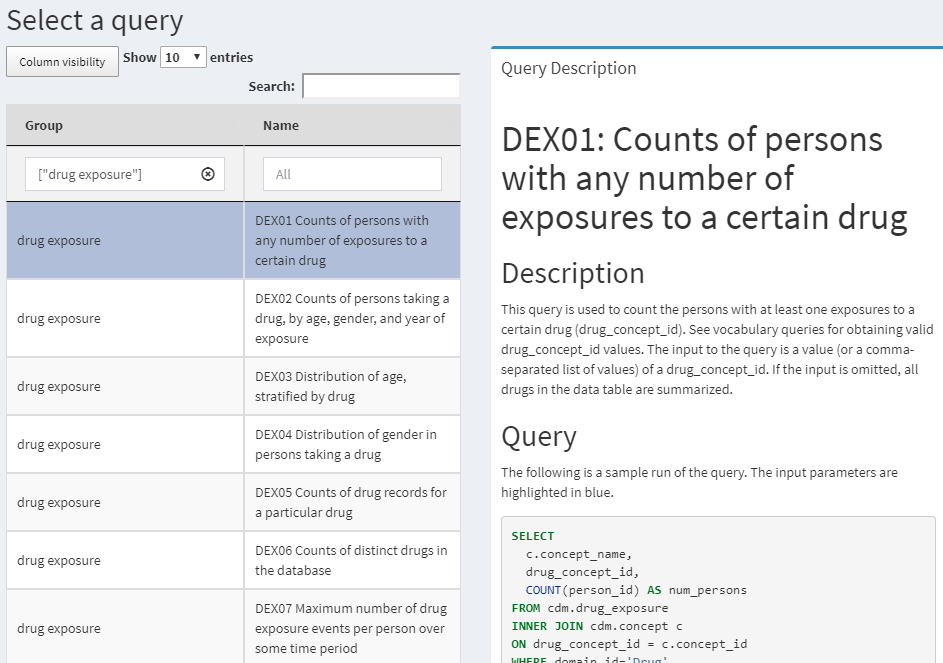
\includegraphics[width=1\linewidth]{images/SqlAndR/queryLibrary} 

}

\caption{クエリライブラリ:CDMに対するSQLクエリのライブラリ。}\label{fig:queryLibrary}
\end{figure}

このライブラリの目的は、新しいユーザーがCDMのクエリ方法を学ぶ手助けをすることです。ライブラリ内のクエリは、OHDSIコミュニティによってレビューされ、承認されています。クエリライブラリは主にトレーニング目的で使用されますが、経験豊富なユーザーにとっても貴重なリソースです。

QueryLibraryは、SqlRenderを使用して、選択したSQLダイアレクトでクエリを出力します。ユーザーはCDMのデータベーススキーマ、語彙のデータベーススキーマ(別々のものがある場合)、およびOracleの一時スキーマ(必要な場合)を指定することもでき、これらの設定でクエリが自動的にレンダリングされます。

\section{簡単な研究のデザイン}\label{ux7c21ux5358ux306aux7814ux7a76ux306eux30c7ux30b6ux30a4ux30f3}

\subsection{問題の定義}\label{ux554fux984cux306eux5b9aux7fa9}

血管浮腫は、ACE阻害剤(ACEi)のよく知られた副作用です。\citet{slater_1988} によると、ACEi治療開始後1週間で血管浮腫の発生率は週あたり3,000人中1例と推定されています。ここでは、この発見を再現し、年齢と性別によって層別化します。簡単のため、1つのACEi(リシノプリル)に焦点を当てます。したがって、次の質問に答えます:

\begin{quote}
リシノプリル治療開始後の最初の1週間での血管浮腫の発生率は、年齢と性別で層別化されていますか?
\end{quote}

\subsection{曝露}\label{ux66ddux9732}

曝露をリシノプリルへの最初の曝露として定義します。最初とは、以前にリシノプリルに曝露されたことがないことを意味します。最初の曝露の前に365日間の連続した観察期間が必要です。

\subsection{アウトカム}\label{ux30a2ux30a6ux30c8ux30abux30e0}

血管浮腫の診断コードが入院または救急(ER)訪問時に出現した場合を血管浮腫の発生と定義します。

\subsection{リスク期間}\label{ux30eaux30b9ux30afux671fux9593}

治療開始後の最初の1週間の発生率を計算します。患者が1週間全部にわたって曝露されているかどうかは問いません。

\section{SQLとRを使用した研究の実施}\label{sqlux3068rux3092ux4f7fux7528ux3057ux305fux7814ux7a76ux306eux5b9fux65bd}

OHDSIツールの規約に縛られることはありませんが、同じ原則に従うと便利です。この場合、OHDSIツールが動作するのと同様に、コホートテーブルを作成するためにSQLを使用します。COHORTテーブルはCDMに定義されており、我々も使用する事前定義されたフィールドセットがあります。まず、書き込み権限のあるデータベーススキーマにCOHORTテーブルを作成する必要がありますが、これはCDM形式でデータを保持しているスキーマとは異なるスキーマである可能性が高いです。

\begin{Shaded}
\begin{Highlighting}[]
\FunctionTok{library}\NormalTok{(DatabaseConnector)}
\NormalTok{conn }\OtherTok{\textless{}{-}} \FunctionTok{connect}\NormalTok{(}\AttributeTok{dbms =} \StringTok{"postgresql"}\NormalTok{,}
                \AttributeTok{server =} \StringTok{"localhost/postgres"}\NormalTok{,}
                \AttributeTok{user =} \StringTok{"joe"}\NormalTok{,}
                \AttributeTok{password =} \StringTok{"secret"}\NormalTok{)}
\NormalTok{cdmDbSchema }\OtherTok{\textless{}{-}} \StringTok{"cdm"}
\NormalTok{cohortDbSchema }\OtherTok{\textless{}{-}} \StringTok{"scratch"}
\NormalTok{cohortTable }\OtherTok{\textless{}{-}} \StringTok{"my\_cohorts"}

\NormalTok{sql }\OtherTok{\textless{}{-}} \StringTok{"}
\StringTok{CREATE TABLE @cohort\_db\_schema.@cohort\_table (}
\StringTok{  cohort\_definition\_id INT,}
\StringTok{  cohort\_start\_date DATE,}
\StringTok{  cohort\_end\_date DATE,}
\StringTok{  subject\_id BIGINT}
\StringTok{);}
\StringTok{"}
\FunctionTok{renderTranslateExecuteSql}\NormalTok{(conn, sql,}
                          \AttributeTok{cohort\_db\_schema =}\NormalTok{ cohortDbSchema,}
                          \AttributeTok{cohort\_table =}\NormalTok{ cohortTable)}
\end{Highlighting}
\end{Shaded}

ここでは、データベーススキーマおよびテーブル名をパラメータ化しているため、異なる環境に簡単に適応できます。結果として、データベースサーバー上に空のテーブルが作成されます。

\subsection{曝露コホート}\label{ux66ddux9732ux30b3ux30dbux30fcux30c8}

次に、曝露コホートを作成し、COHORTテーブルに挿入します:

\begin{Shaded}
\begin{Highlighting}[]
\NormalTok{sql }\OtherTok{\textless{}{-}} \StringTok{"}
\StringTok{INSERT INTO @cohort\_db\_schema.@cohort\_table (}
\StringTok{  cohort\_definition\_id,}
\StringTok{  cohort\_start\_date,}
\StringTok{  cohort\_end\_date,}
\StringTok{  subject\_id}
\StringTok{)}
\StringTok{SELECT 1 AS cohort\_definition\_id,}
\StringTok{  cohort\_start\_date,}
\StringTok{  cohort\_end\_date,}
\StringTok{  subject\_id}
\StringTok{FROM (}
\StringTok{  SELECT drug\_era\_start\_date AS cohort\_start\_date,}
\StringTok{    drug\_era\_end\_date AS cohort\_end\_date,}
\StringTok{    person\_id AS subject\_id}
\StringTok{  FROM (}
\StringTok{    SELECT drug\_era\_start\_date,}
\StringTok{      drug\_era\_end\_date,}
\StringTok{      person\_id,}
\StringTok{      ROW\_NUMBER() OVER (}
\StringTok{        PARTITION BY person\_id}
\StringTok{            ORDER BY drug\_era\_start\_date}
\StringTok{      ) order\_nr}
\StringTok{    FROM @cdm\_db\_schema.drug\_era}
\StringTok{    WHERE drug\_concept\_id = 1308216 {-}{-} リシノプリル}
\StringTok{  ) ordered\_exposures}
\StringTok{  WHERE order\_nr = 1}
\StringTok{) first\_era}
\StringTok{INNER JOIN @cdm\_db\_schema.observation\_period}
\StringTok{  ON subject\_id = person\_id}
\StringTok{    AND observation\_period\_start\_date \textless{} cohort\_start\_date}
\StringTok{    AND observation\_period\_end\_date \textgreater{} cohort\_start\_date}
\StringTok{WHERE DATEDIFF(DAY,}
\StringTok{               observation\_period\_start\_date,}
\StringTok{               cohort\_start\_date) \textgreater{}= 365;}
\StringTok{"}

\FunctionTok{renderTranslateExecuteSql}\NormalTok{(conn, sql,}
                          \AttributeTok{cohort\_db\_schema =}\NormalTok{ cohortDbSchema,}
                          \AttributeTok{cohort\_table =}\NormalTok{ cohortTable,}
                          \AttributeTok{cdm\_db\_schema =}\NormalTok{ cdmDbSchema)}
\end{Highlighting}
\end{Shaded}

ここでは、CDMの標準テーブルであるDRUG\_ERAテーブルを使用します。このテーブルはDRUG\_EXPOSUREテーブルから自動的に派生されます。DRUG\_ERAテーブルには連続する成分レベルの曝露期間が含まれるため、リシノプリルを検索すると、自動的にリシノプリルを含む薬物のすべての曝露を特定します。各人の最初の薬剤曝露を選択し、OBSERVATION\_PERIODテーブルと結合します。各人が複数の観察期間を持つことができるため、薬剤曝露を含む期間にのみ結合されるよう注意が必要です。一方で、OBSERVATION\_PERIOD\_START\_DATEとCOHORT\_START\_DATEの間に少なくとも365日の間隔を要求します。

\subsection{アウトカムコホート}\label{ux30a2ux30a6ux30c8ux30abux30e0ux30b3ux30dbux30fcux30c8}

最後に、アウトカムコホートを作成する必要があります:

\begin{Shaded}
\begin{Highlighting}[]
\NormalTok{sql }\OtherTok{\textless{}{-}} \StringTok{"}
\StringTok{INSERT INTO @cohort\_db\_schema.@cohort\_table (}
\StringTok{ cohort\_definition\_id,}
\StringTok{ cohort\_start\_date,}
\StringTok{ cohort\_end\_date,}
\StringTok{subject\_id}
\StringTok{)}
\StringTok{SELECT 2 AS cohort\_definition\_id,}
\StringTok{  cohort\_start\_date,}
\StringTok{  cohort\_end\_date,}
\StringTok{  subject\_id}
\StringTok{FROM (}
\StringTok{  SELECT DISTINCT person\_id AS subject\_id,}
\StringTok{    condition\_start\_date AS cohort\_start\_date,}
\StringTok{    condition\_end\_date AS cohort\_end\_date}
\StringTok{  FROM @cdm\_db\_schema.condition\_occurrence}
\StringTok{  INNER JOIN @cdm\_db\_schema.concept\_ancestor}
\StringTok{    ON condition\_concept\_id = descendant\_concept\_id}
\StringTok{  WHERE ancestor\_concept\_id = 432791 {-}{-} 血管浮腫}
\StringTok{) distinct\_occurrence}
\StringTok{INNER JOIN @cdm\_db\_schema.visit\_occurrence}
\StringTok{  ON subject\_id = person\_id}
\StringTok{  AND visit\_start\_date \textless{}= cohort\_start\_date}
\StringTok{  AND visit\_end\_date \textgreater{}= cohort\_start\_date}
\StringTok{WHERE visit\_concept\_id IN (262, 9203,}
\StringTok{    9201) {-}{-} 入院またはER;}
\StringTok{"}

\FunctionTok{renderTranslateExecuteSql}\NormalTok{(conn, sql,}
                          \AttributeTok{cohort\_db\_schema =}\NormalTok{ cohortDbSchema,}
                          \AttributeTok{cohort\_table =}\NormalTok{ cohortTable,}
                          \AttributeTok{cdm\_db\_schema =}\NormalTok{ cdmDbSchema)}
\end{Highlighting}
\end{Shaded}

ここでは、CONDITION\_OCCURRENCEテーブルをCONCEPT\_ANCESTORテーブルと結合して、血管浮腫またはその子孫のすべての発生を見つけます。同じ日に複数の診断がある場合、それは同じ現象である可能性が高いため、各日1件のレコードのみを取得するようにDISTINCTを使用します。次に、診断が入院またはERで行われたことを確認するために、これらの発生をVISIT\_OCCURRENCEテーブルと結合します。

\subsection{発症率の計算}\label{ux767aux75c7ux7387ux306eux8a08ux7b97}

コホートが整ったので、年齢と性別に分けて発症率を計算できます:

\begin{Shaded}
\begin{Highlighting}[]
\NormalTok{sql }\OtherTok{\textless{}{-}} \StringTok{"}
\StringTok{WITH tar AS (}
\StringTok{  SELECT concept\_name AS gender,}
\StringTok{    FLOOR((YEAR(cohort\_start\_date) {-}}
\StringTok{          year\_of\_birth) / 10) AS age,}
\StringTok{    subject\_id,}
\StringTok{    cohort\_start\_date,}
\StringTok{    CASE WHEN DATEADD(DAY, 7, cohort\_start\_date) \textgreater{}}
\StringTok{      observation\_period\_end\_date}
\StringTok{    THEN observation\_period\_end\_date}
\StringTok{    ELSE DATEADD(DAY, 7, cohort\_start\_date)}
\StringTok{    END AS cohort\_end\_date}
\StringTok{  FROM @cohort\_db\_schema.@cohort\_table}
\StringTok{  INNER JOIN @cdm\_db\_schema.observation\_period}
\StringTok{    ON subject\_id = observation\_period.person\_id}
\StringTok{      AND observation\_period\_start\_date \textless{} cohort\_start\_date}
\StringTok{      AND observation\_period\_end\_date \textgreater{} cohort\_start\_date}
\StringTok{  INNER JOIN @cdm\_db\_schema.person}
\StringTok{    ON subject\_id = person.person\_id}
\StringTok{  INNER JOIN @cdm\_db\_schema.concept}
\StringTok{    ON gender\_concept\_id = concept\_id}
\StringTok{  WHERE cohort\_definition\_id = 1 {-}{-} 曝露}
\StringTok{)}
\StringTok{SELECT days.gender,}
\StringTok{    days.age,}
\StringTok{    days,}
\StringTok{    CASE WHEN events IS NULL THEN 0 ELSE events END AS events}
\StringTok{FROM (}
\StringTok{  SELECT gender,}
\StringTok{    age,}
\StringTok{    SUM(DATEDIFF(DAY, cohort\_start\_date,}
\StringTok{      cohort\_end\_date)) AS days}
\StringTok{  FROM tar}
\StringTok{  GROUP BY gender,}
\StringTok{    age}
\StringTok{) days}
\StringTok{LEFT JOIN (}
\StringTok{  SELECT gender,}
\StringTok{      age,}
\StringTok{      COUNT(*) AS events}
\StringTok{  FROM tar}
\StringTok{  INNER JOIN @cohort\_db\_schema.@cohort\_table angioedema}
\StringTok{    ON tar.subject\_id = angioedema.subject\_id}
\StringTok{      AND tar.cohort\_start\_date \textless{}= angioedema.cohort\_start\_date}
\StringTok{      AND tar.cohort\_end\_date \textgreater{}= angioedema.cohort\_start\_date}
\StringTok{  WHERE cohort\_definition\_id = 2 {-}{-} 結果}
\StringTok{  GROUP BY gender,}
\StringTok{    age}
\StringTok{) events}
\StringTok{ON days.gender = events.gender}
\StringTok{  AND days.age = events.age;}
\StringTok{"}

\NormalTok{results }\OtherTok{\textless{}{-}} \FunctionTok{renderTranslateQuerySql}\NormalTok{(conn, sql,}
                                   \AttributeTok{cohort\_db\_schema =}\NormalTok{ cohortDbSchema,}
                                   \AttributeTok{cohort\_table =}\NormalTok{ cohortTable,}
                                   \AttributeTok{cdm\_db\_schema =}\NormalTok{ cdmDbSchema,}
                                   \AttributeTok{snakeCaseToCamelCase =} \ConstantTok{TRUE}\NormalTok{)}
\end{Highlighting}
\end{Shaded}

まず、CTE「tar」を作成し、適切なリスク時間を伴うすべての曝露を含めます。OBSERVATION\_PERIOD\_END\_DATEでリスク時間を切り詰めることに注意してください。また、10年ごとの年齢階層を計算し、性別を特定します。CTEを使用する利点は、クエリ中に同じ中間結果セットを複数回使用できることです。この場合、リスク時間の合計およびリスク期間中に発生する血管浮腫の数を数えるために使用します。

SQLではフィールド名にスネークケースを使用するため(SQLは大文字小文字を区別しないため)、Rではキャメルケースを使用します(Rは大文字小文字を区別するため)。\texttt{results}データフレームの列名はキャメルケースになります。

ggplot2パッケージを使用すると、結果を簡単にプロットできます:

\begin{Shaded}
\begin{Highlighting}[]
\CommentTok{\# 発症率(IR)を計算}
\NormalTok{results}\SpecialCharTok{$}\NormalTok{ir }\OtherTok{\textless{}{-}} \DecValTok{1000} \SpecialCharTok{*}\NormalTok{ results}\SpecialCharTok{$}\NormalTok{events }\SpecialCharTok{/}\NormalTok{ results}\SpecialCharTok{$}\NormalTok{days }\SpecialCharTok{/} \DecValTok{7}

\CommentTok{\# 年齢スケールを修正}
\NormalTok{results}\SpecialCharTok{$}\NormalTok{age }\OtherTok{\textless{}{-}}\NormalTok{ results}\SpecialCharTok{$}\NormalTok{age }\SpecialCharTok{*} \DecValTok{10}

\FunctionTok{library}\NormalTok{(ggplot2)}
\FunctionTok{ggplot}\NormalTok{(results, }\FunctionTok{aes}\NormalTok{(}\AttributeTok{x =}\NormalTok{ age, }\AttributeTok{y =}\NormalTok{ ir, }\AttributeTok{group =}\NormalTok{ gender, }\AttributeTok{color =}\NormalTok{ gender)) }\SpecialCharTok{+}
  \FunctionTok{geom\_line}\NormalTok{() }\SpecialCharTok{+}
  \FunctionTok{xlab}\NormalTok{(}\StringTok{"年齢"}\NormalTok{) }\SpecialCharTok{+}
  \FunctionTok{ylab}\NormalTok{(}\StringTok{"発症率(1,000患者週間当たり)"}\NormalTok{)}
\end{Highlighting}
\end{Shaded}

\begin{center}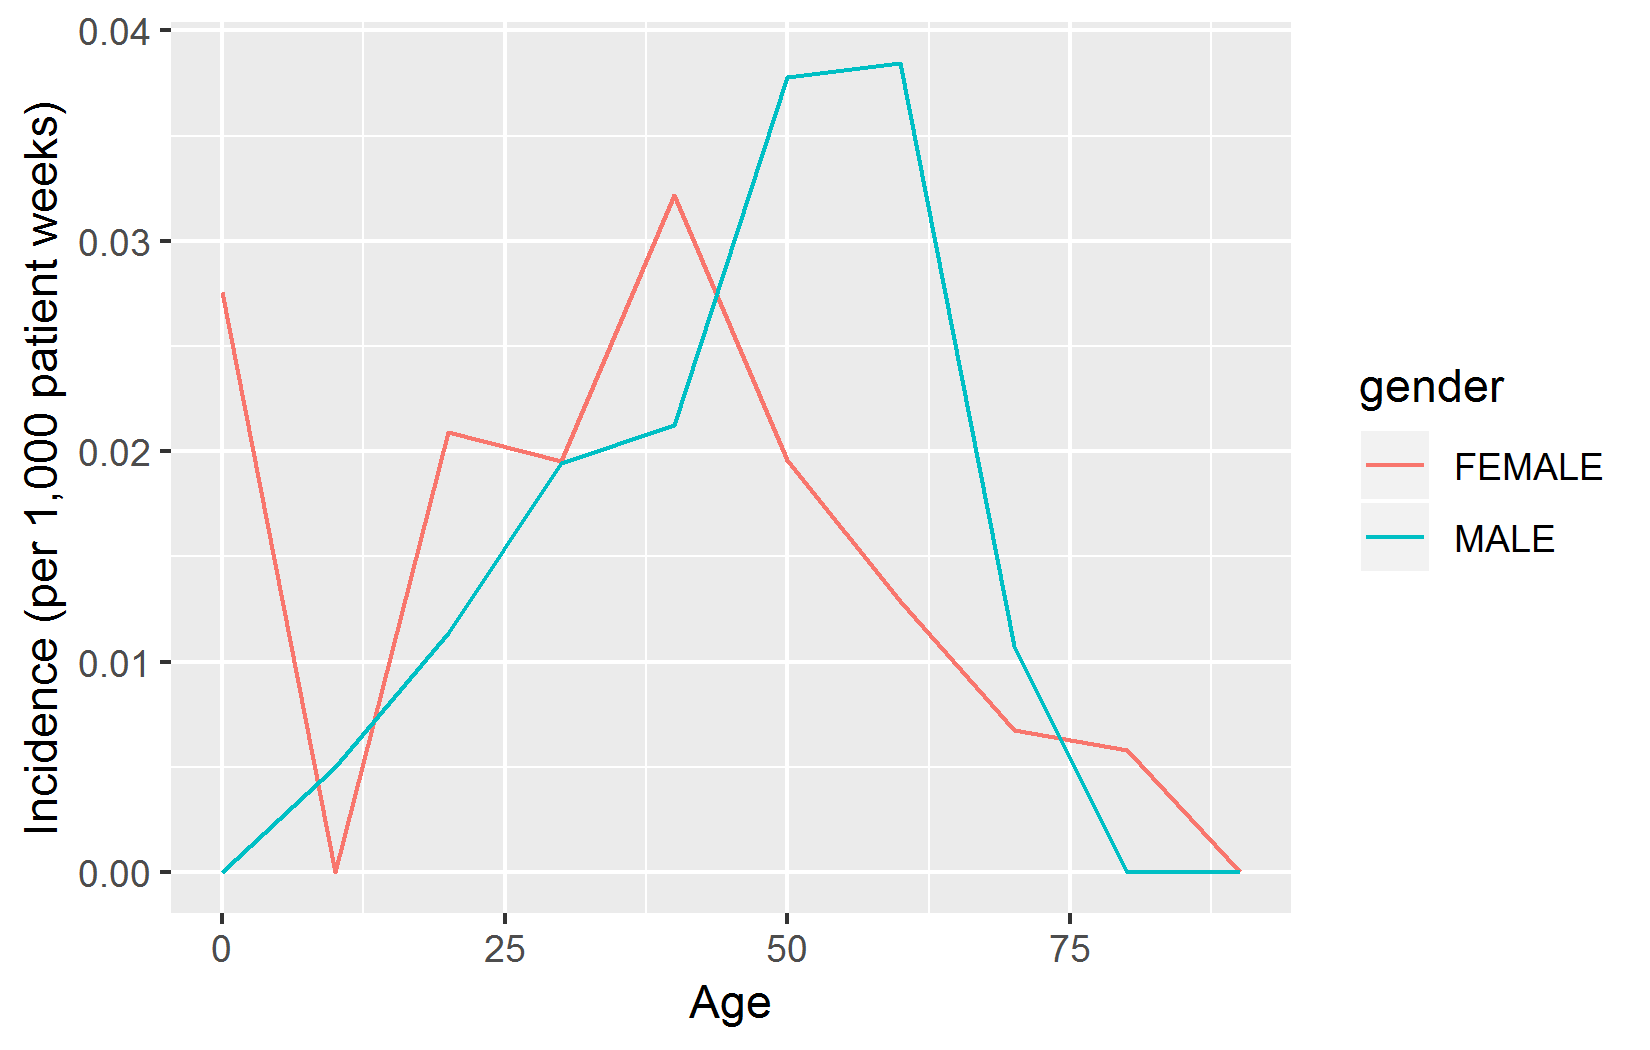
\includegraphics[width=0.8\linewidth]{images/SqlAndR/ir} \end{center}

\subsection{クリーンアップ}\label{ux30afux30eaux30fcux30f3ux30a2ux30c3ux30d7}

作成したテーブルをクリーンアップし、接続を閉じることを忘れないでください:

\begin{Shaded}
\begin{Highlighting}[]
\NormalTok{sql }\OtherTok{\textless{}{-}} \StringTok{"}
\StringTok{TRUNCATE TABLE @cohort\_db\_schema.@cohort\_table;}
\StringTok{DROP TABLE @cohort\_db\_schema.@cohort\_table;}
\StringTok{"}
\FunctionTok{renderTranslateExecuteSql}\NormalTok{(conn, sql,}
                          \AttributeTok{cohort\_db\_schema =}\NormalTok{ cohortDbSchema,}
                          \AttributeTok{cohort\_table =}\NormalTok{ cohortTable)}

\FunctionTok{disconnect}\NormalTok{(conn)}
\end{Highlighting}
\end{Shaded}

\subsection{互換性}\label{ux4e92ux63dbux6027}

OHDSI SQLとDatabaseConnectorおよびSqlRenderを組み合わせて使用するため、ここで紹介したコードはOHDSIがサポートする任意のデータベースプラットフォームで実行できます。

デモンストレーションの目的で、手作業で作成したSQLを使用してコホートを作成することを選びましたが、ATLASでコホート定義を構築し、ATLASが生成したSQLを使用してコホートを実インスタンス化する方が便利です。ATLASもOHDSI SQLを生成し、SqlRenderおよびDatabaseConnectorと一緒に簡単に使用できます。

\section{まとめ}\label{ux307eux3068ux3081-7}

\begin{rmdsummary}
\begin{itemize}
\item
  \textbf{SQL}(Structured Query Language)は、共通データモデル(CDM)に準拠したデータベースを含む、データベースを照会するための標準言語です。
\item
  異なるデータベースプラットフォームは異なるSQL表現を持っており、照会するためには異なるツールが必要です。
\item
  \textbf{SqlRender}および\textbf{DatabaseConnector}Rパッケージは、CDM内のデータを照会するための統一された方法を提供し、同じ分析コードを異なる環境で変更なしで実行できるようにします。
\item
  RとSQLを組み合わせて使用することで、OHDSIツールではサポートされていないカスタム分析を実装できます。
\item
  \textbf{QueryLibrary}は、CDM用の再利用可能なSQLクエリのコレクションを提供します。
\end{itemize}
\end{rmdsummary}

\section{練習問題}\label{ux7df4ux7fd2ux554fux984c-1}

\subsubsection*{前提条件}\label{ux524dux63d0ux6761ux4ef6-3}
\addcontentsline{toc}{subsubsection}{前提条件}

これらの練習問題では、セクション \ref{installR} に記載されているように、R、R-Studio、Java がインストールされていることを前提とします。また、\href{https://ohdsi.github.io/SqlRender/}{SqlRender}、\href{https://ohdsi.github.io/DatabaseConnector/}{DatabaseConnector}、および \href{https://ohdsi.github.io/Eunomia/}{Eunomia} パッケージも必要です。以下の手順でインストールできます。

\begin{Shaded}
\begin{Highlighting}[]
\FunctionTok{install.packages}\NormalTok{(}\FunctionTok{c}\NormalTok{(}\StringTok{"SqlRender"}\NormalTok{, }\StringTok{"DatabaseConnector"}\NormalTok{, }\StringTok{"remotes"}\NormalTok{))}
\NormalTok{remotes}\SpecialCharTok{::}\FunctionTok{install\_github}\NormalTok{(}\StringTok{"ohdsi/Eunomia"}\NormalTok{, }\AttributeTok{ref =} \StringTok{"v1.0.0"}\NormalTok{)}
\end{Highlighting}
\end{Shaded}

Eunomia パッケージは、CDM 内でローカル R セッション内で動作するシミュレートされたデータセットを提供します。接続の詳細は以下の方法で取得できます。

\begin{Shaded}
\begin{Highlighting}[]
\NormalTok{connectionDetails }\OtherTok{\textless{}{-}}\NormalTok{ Eunomia}\SpecialCharTok{::}\FunctionTok{getEunomiaConnectionDetails}\NormalTok{()}
\end{Highlighting}
\end{Shaded}

CDM データベースのスキーマは「main」です。

\begin{exercise}
\protect\hypertarget{exr:exercisePeopleCount}{}\label{exr:exercisePeopleCount}SQL および R を使用して、データベース内に何人いるかを計算しなさい。
\end{exercise}

\begin{exercise}
\protect\hypertarget{exr:exerciseCelecoxibUsers}{}\label{exr:exerciseCelecoxibUsers}SQL および R を使用して、少なくとも 1 回のセレコキシブの処方を受けたことがある人の数を計算しなさい。
\end{exercise}

\begin{exercise}
\protect\hypertarget{exr:exerciseGiBleedsDuringCelecoxib}{}\label{exr:exerciseGiBleedsDuringCelecoxib}SQL および R を使用して、セレコキシブの服用中に胃腸出血の診断が出たケースの数を計算しなさい。(ヒント: 胃腸出血のコンセプト ID は \href{http://athena.ohdsi.org/search-terms/terms/192671}{192671} です)
\end{exercise}

提案された解答は付録 \ref{SqlAndRanswers} にあります。

\chapter{第10章 --翻訳作業中-- コホートの定義}\label{Cohorts}

\emph{章のリード: Kristin Kostka!}

観察型健康データ(\emph{リアルワールドデータ}とも呼ばれる)は、患者の健康状態や医療の提供に関連するデータで、さまざまな情報源から日常的に収集されたデータです。そのため、OHDSIデータスチュワード(OHDSIの共同研究者で、各サイトのCDMにデータを維持している人々)は、電子健康記録(EHR)、健康保険請求データ、製品や疾患のレジストリ、自宅使用環境を含む患者が生成したデータ、および携帯端末など健康状態に関する情報を提供できる他の情報源など、複数の情報源からデータをキャプチャする場合があります。これらのデータは研究目的で収集されたものではないため、興味のある臨床データ要素を明示的にキャプチャしていない場合があります。

たとえば、健康保険の請求データベースは、あるコンディション(例:血管浮腫)に対して提供されたすべてのケアをキャプチャして関連コストが適切に補償されるように設計されており、実際のコンディションに関する情報はこの目的の一環としてのみキャプチャされます。このような観察データを研究目的で使用したい場合、データにキャプチャされているものを使用して本当に興味のあるものを推測するためのロジックを作成する必要があります。つまり、臨床イベントがどのように現れるかの定義を使用してコホートを作成する必要があるのです。たとえば、保険請求データベースで血管浮腫イベントを特定したい場合、血管浮腫の診断コードが緊急室の設定で記録されていることを要求するロジックを定義し、過去の血管浮腫の発生に対するフォローアップケアを単に説明する請求から区別するかもしれません。類似の考慮事項は、EHRに記録された日常的な医療の相互作用でキャプチャされるデータに対しても適用されます。データが二次的な目的で使用されているため、各データベースが元々何を目的として設計されたかを認識する必要があります。研究を設計するたびに、さまざまな医療環境でコホートがどのように存在するのかについての細かな点を考慮する必要があります。

この章では、コホート定義の作成と共有とは何か、コホートを開発する方法、およびATLASまたはSQLを使用して独自のコホートを作成する方法について説明します。

\section{コホートとは?}\label{ux30b3ux30dbux30fcux30c8ux3068ux306f}

OHDSI研究では、コホートを一つ以上の包含基準を満たし、一定期間にわたってこれを維持している人々の集合として定義します。この用語はしばしば\emph{フェノタイプ}と置き換えられます。コホートは、OHDSI分析ツールやネットワーク研究全体で研究質問を実行するための主要な構成要素として使用されます。たとえば、ACE阻害薬の開始による血管浮腫リスクを予測することを目的とした研究では、2つのコホートを定義します:アウトカムコホート(血管浮腫)およびターゲットコホート(ACE阻害薬を開始する人々)。OHDSIのコホートの重要な側面は、通常、研究内の他のコホートから独立して定義されるため、再利用が可能であることです。たとえば、血管浮腫コホートはターゲット集団外も含む集団全体のすべての血管浮腫イベントを特定します。分析時に必要に応じてこれらの二つのコホートの交差を取ります。この利点は、同じ血管浮腫コホート定義が、たとえばACE阻害薬と他の曝露を比較する推定研究など、他の分析でも使用できるということです。コホート定義は、研究の質問に応じて異なることがあります。

\begin{rmdimportant}
コホートは、一つ以上の包含基準を満たし、それを一定期間維持する人々の集合です。
\end{rmdimportant}

\index{コホート} \index{コホート定義} OHDSIで使用されるコホートの定義は、この分野の他の人々が使用するものとは異なるかもしれないことを理解することが重要です。たとえば、多くの査読済み科学論文では、コホートが特定の臨床コードのコードセット(例:ICD-9/ICD-10、NDC、HCPCSなど)に類似していると示唆されることがあります。コードセットはコホートを組み立てる際の重要な要素ですが、コホートはコードセットによって定義されません。コホートは、条件を満たすコードセットの使用方法に関する具体的なロジックを必要とします(例:これはICD-9/ICD-10コードの最初の発生ですか?任意の発生ですか?)。 よく定義されたコホートは、患者がコホートに入る方法とコホートから退出する方法を指定します。 \index{コードセット}

\index{フェノタイプ} OHDSIのコホート定義を利用するためのユニークなニュアンスには以下があります:

\begin{itemize}
\tightlist
\item
  一人の人が複数のコホートに属する可能性があります
\item
  一人の人が同じコホートに異なる期間属する可能性があります
\item
  一人の人が同じ期間内に同じコホートに複数回属することはありません
\item
  コホートにはメンバーがゼロまたは複数いる場合があります
\end{itemize}

コホートを構築するための主要なアプローチは二つあります:

\begin{enumerate}
\def\labelenumi{\arabic{enumi}.}
\item
  \textbf{ルールベースのコホート定義} は、患者がコホートにいる時期を明示的なルールで説明します。これらのルールを定義するには通常、コホートの包含基準のルールを構築するために、対象となる治療領域の知識を持つ個人のドメインの専門知識に大きく依存する。
\item
  \textbf{確率的コホート定義} は、コホートにいる患者の確率(0から100\%の間の確率)を計算する確率モデルを使用します。この確率は、しきい値を使用してイエス・ノーの分類に変換できるか、または一部の研究デザインではそのまま使用できます。確率モデルは通常、機械学習(例:ロジスティック回帰)を使用して、関連する患者特性を自動的に特定するために例データでトレーニングされます。
\end{enumerate}

次のセクションでは、これらのアプローチについて詳しく説明します。

\section{ルールベースのコホート定義}\label{ux30ebux30fcux30ebux30d9ux30fcux30b9ux306eux30b3ux30dbux30fcux30c8ux5b9aux7fa9}

ルールベースのコホート定義は、特定の期間内に明示的に一つ以上の包含基準(例:「血管浮腫のある人」)を定義することから始まります(例:「過去6ヶ月以内にこの状態を発症した人」)。\index{cohort!rule-based design}

これらの基準を組み立てるために使用する標準的なコンポーネントは次のとおりです:

\begin{itemize}
\item
  \textbf{ドメイン}:データが保存されているCDMドメイン(例:「処置の発生」、「薬剤曝露」)は、臨床情報の種類およびそのCDMテーブル内に表現可能なコンセプトを定義します。ドメインについては、セクション\ref{domains}で詳しく説明されています。
\item
  \textbf{コンセプトセット}:臨床実体を包含する一つ以上の標準コンセプトを定義するデータ非依存の表現です。これらのコンセプトセットは、異なる観察健康データ間で相互運用可能であり、ボキャブラリ内の標準用語にマッピングされる臨床実体を表します。コンセプトセットについては、セクション\ref{conceptSets}で詳しく説明されています。
\item
  \textbf{ドメイン固有の属性}:関心のある臨床実体に関連する追加の属性(例:DRUG\_EXPOSUREのDAYS\_SUPPLYやMEASUREMENTのVALUE\_AS\_NUMBERやRANGE\_HIGH)。
\item
  \textbf{時間ロジック}:包含基準とイベントとの関係を評価する時間間隔(例:指定された状態は曝露開始の365日前またはその日前後で発生する必要があります)。
\end{itemize}

コホート定義を構築する際、コホート属性を表すブロックのようにドメインを考えると便利です(図\ref{fig:cohortLegos}参照)。各ドメインの許容内容について混乱した場合は、共通データモデルの章(チャプター\ref{CommonDataModel})を参照してください。

\begin{figure}

{\centering 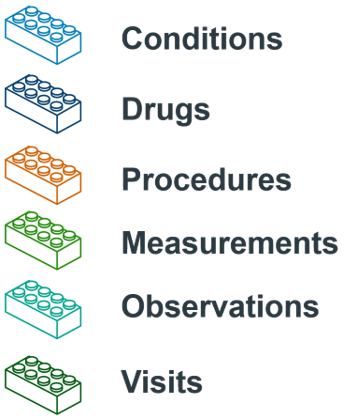
\includegraphics[width=0.5\linewidth]{images/Cohorts/cohort-legos} 

}

\caption{コホート定義のブロック}\label{fig:cohortLegos}
\end{figure}

コホート定義作成時に自問すべきいくつかの質問があります:

\begin{itemize}
\tightlist
\item
  \emph{コホートエントリの時間を定義する初期イベントは何か?}
\item
  \emph{初期イベントに適用される包含基準は何か?}
\item
  \emph{コホート退出の時間を定義するものは何か?}
\end{itemize}

\textbf{コホートエントリエベント}:コホートエントリエベント(初期イベント)は、人々がコホートに参加する時点、つまり\textbf{コホートインデックス日}を定義します。コホートエントリエベントは、薬剤曝露、コンディション、処置、測定値、受診期間など、CDMで記録された任意のイベントであり得ます。初期イベントは、データが保存されているCDMドメイン(例:PROCEDURE\_OCCURRENCE、DRUG\_EXPOSUREなど)、臨床活動を特定するために作成されたコンセプトセット(例:状態のためのSNOMEDコード、薬剤のためのRxNormコード)、およびその他の特定の属性(例:発生時の年齢、初診断/処置/その他、開始日と終了日の指定、受診期間または基準の指定、供給日数など)によって定義されます。エントリエベントを持つ人々のセットは\textbf{初期イベントコホート}と呼ばれます。\index{cohort!entry event}

\textbf{包含基準}:包含基準は、初期イベントコホートに適用され、さらに人々のセットを制限します。各包含基準は、データが保存されているCDMドメイン、臨床活動を表すコンセプトセット、ドメイン固有の属性(例:供給日数、受診期間など)、およびコホートインデックス日相対の時間論理によって定義されます。各包含基準は、初期イベントコホートからの人々の脱落に対する基準の影響を評価するために使用されます。\textbf{適格コホート}は、すべての包含基準を満たす初期イベントコホート内のすべての人々として定義されます。\index{cohort!inclusion criteria}

\textbf{コホート退出基準}:コホート退出イベントは、ある人がコホート会員資格を失う時点を示します。コホート退出は、観察期間の終了、初期エントリエベント相対の固定時間間隔、関連する観察の一連の最後のイベント(例:持続的な薬剤曝露)または観察期間の他の打ち切りによって定義される場合があります。コホート退出戦略は、ある人が異なる時間間隔で複数回コホートに属することができるかどうかに影響を与えます。 \index{cohort!exit criteria}

\begin{rmdimportant}
OHDSIツールでは、包含基準と除外基準の区別はありません。すべての基準は包含基準として形式化されます。例えば、「以前の高血圧のある人を除外する」という除外基準は、「以前の高血圧の発生が0回の人を含む」という包含基準として形式化されます。
\end{rmdimportant}

\section{コンセプトセット}\label{conceptSets}

\index{concept set}

コンセプトセットは、さまざまな分析で再利用可能なコンポーネントとして使用できるコンセプトのリストを表す表現です。これは、観察研究でよく使用されるコードリストの標準化されたコンピュータ実行可能な同等物と考えることができます。コンセプトセットの表現は、次の属性を持つコンセプトのリストで構成されます:

\begin{itemize}
\tightlist
\item
  \textbf{除外}:このコンセプト(および選択された場合はその子孫)をコンセプトセットから除外します。
\item
  \textbf{子孫}:このコンセプトだけでなく、その子孫も考慮します。
\item
  \textbf{マッピング対象}:非標準コンセプトを検索することを許可します。
\end{itemize}

例えば、コンセプトセットの表現は、図に示されるように2つのコンセプトを含むことができます(表\ref{tab:conceptSetExpression})。ここでは、コンセプト\href{http://athena.ohdsi.org/search-terms/terms/4329847}{4329847}(「心筋梗塞」)およびそのすべての子孫を含む一方、コンセプト\href{http://athena.ohdsi.org/search-terms/terms/314666}{314666}(「古い心筋梗塞」)およびそのすべての子孫を除外します。

表:(\#tab:conceptSetExpression)コンセプトセットの表現の例。

\begin{longtable}[]{@{}lclll@{}}
\toprule\noalign{}
コンセプトID & コンセプト名 & 除外 & 子孫 & マッピング対象 \\
\midrule\noalign{}
\endhead
\bottomrule\noalign{}
\endlastfoot
4329847 & 心筋梗塞 & いいえ & はい & いいえ \\
314666 & 古い心筋梗塞 & はい & はい & いいえ \\
\end{longtable}

図に示すように(図\ref{fig:conceptSet})、これは「心筋梗塞」およびその子孫を含むが、「古い心筋梗塞」およびその子孫は除外します。全体で、このコンセプトセットの表現は、ほぼ100の標準コンセプトを意味します。これらの標準コンセプトは、さまざまなデータベースに表示されるかもしれない何百ものソースコード(例:ICD-9およびICD-10コード)を反映します。

\begin{figure}

{\centering 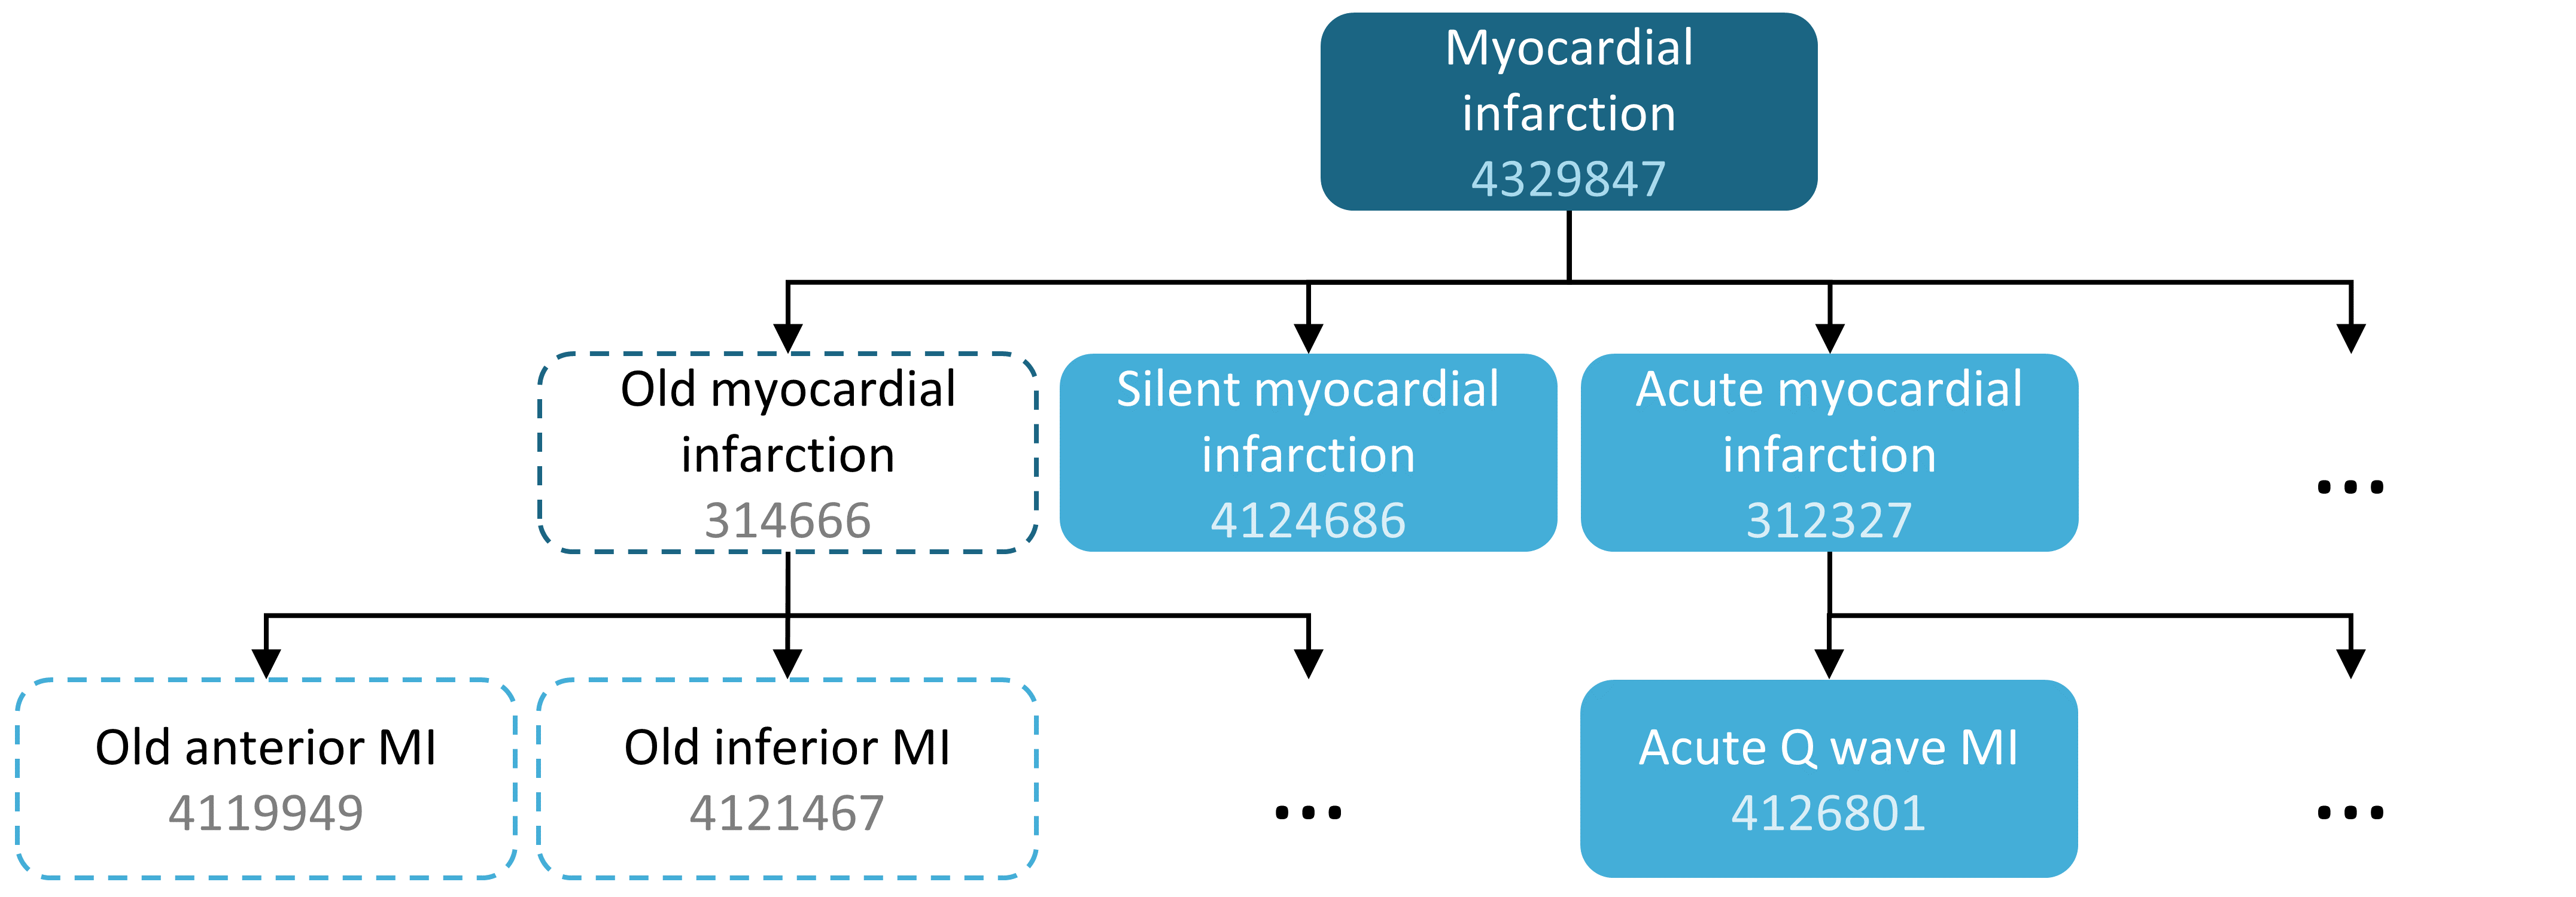
\includegraphics[width=1\linewidth]{images/Cohorts/conceptSet} 

}

\caption{「心筋梗塞」(子孫を含む)を含むが、「古い心筋梗塞」(子孫を含む)を除外するコンセプトセット。}\label{fig:conceptSet}
\end{figure}

\section{確率的コホート定義}\label{ux78baux7387ux7684ux30b3ux30dbux30fcux30c8ux5b9aux7fa9}

ルールベースのコホート定義は、コホート定義を組み立てるための一般的な方法です。しかし、研究コホートを作成するために必要な専門家の合意を集めることは非常に時間がかかります。確率的コホート設計は、コホート属性の選択を迅速化するための代替手段であり、機械主導の方法です。このアプローチでは、監督された機械学習により、フェノタイピングアルゴリズムがコホート会員資格に寄与する属性がどのようにラベル付けされた例(ケース)から学習します。次に、このアルゴリズムを使用して、フェノタイプを定義する特性をより明確にし、フェノタイプ基準を変更する際に全体的な研究精度でどのようなトレードオフが発生するかを判断できます。 \index{cohort!probabilistic design}

このアプローチをCDMデータに適用する例は、APHRODITE(自動フェノタイプルーチンオブザーバーション定義、識別、トレーニングおよび評価)Rパッケージ\footnote{\url{https://github.com/OHDSI/Aphrodite}}です。このパッケージは、不完全にラベル付けされたデータから学習する能力を組み合わせたコホートビルディングフレームワークを提供します \citep{Banda2017APHRODITE} \index{APHRODITE}。

\section{コホート定義の妥当性}\label{ux30b3ux30dbux30fcux30c8ux5b9aux7fa9ux306eux59a5ux5f53ux6027}

コホートを構築する際には次のどちらが重要かを考慮すべきです:\emph{すべての該当患者を見つけることが重要か?} それとも \emph{確信を持てる患者のみを取り込むことが重要か?}

コホートの構築戦略は、専門家のコンセンサスが疾患をどのように定義するかの臨床的厳格性に依存します。これはつまり、正しいコホート設計はあなたが解答を求めている質問に依存するということです。すべてを取り入れるコホート定義を選択するか、OHDSIサイト全体で共有できる最小公約数を使用するか、またはその両者の妥協案を選ぶか。最終的には、研究者の判断により、対象コホートの適切な研究に必要な厳格性の閾値が決まります。

この章の冒頭で述べたように、コホート定義は記録されたデータから観察したいことを推測する試みです。それがどの程度うまくいったかという問いが生じます。一般に、ルールに基づくコホート定義や確率的アルゴリズムの検証は、提案されたコホートを「ゴールドスタンダード」の参照(例: ケースの手動チャートレビュー)と比較する試験として考えられます。詳細はChapter \ref{ClinicalValidity}(「臨床的妥当性」)に記載されています。

\subsection{OHDSI ゴールドスタンダード表現型ライブラリ}\label{ohdsi-ux30b4ux30fcux30ebux30c9ux30b9ux30bfux30f3ux30c0ux30fcux30c9ux8868ux73feux578bux30e9ux30a4ux30d6ux30e9ux30ea}

既存のコホート定義とアルゴリズムの在庫と全体的な評価を支援するために、OHDSI ゴールドスタンダード表現型ライブラリ(GSPL)ワーキンググループが設立されました。GSPLワーキンググループの目的は、ルールベースおよび確率的手法からのコミュニティ支援のフェノタイプライブラリを開発することです。GSPLにより、OHDSIコミュニティのメンバーは、コミュニティによって検証されたコホート定義を研究やその他の活動に利用することができます。これらの「ゴールドスタンダード」定義は特定の設計と評価基準に従ってライブラリに保存されます。GSPLに関連する追加情報はOHDSIワーキンググループページを参照してください。\footnote{\url{https://www.ohdsi.org/web/wiki/doku.php?id=projects:workgroups:gold-library-wg}} このワーキンググループの研究には、先のセクションで議論されたAPHRODITE \citep{Banda2017APHRODITE} およびPheValuatorツール \citep{Swerdel2019phevaluator} の他、OHDSIネットワーク全体での電子カルテおよびゲノミクスの \href{https://emerge.mc.vanderbilt.edu/}{eMERGE} \href{https://phekb.org/phenotypes}{Phenotype Library} の共有に関する作業も含まれます \citep{Hripcsak2019eMERGE}。表現型のキュレーションに関心がある場合は、このワーキンググループに貢献することを考えてみてください。 \index{phenotype library}

\section{高血圧のコホート定義}\label{ux9ad8ux8840ux5727ux306eux30b3ux30dbux30fcux30c8ux5b9aux7fa9}

コホート定義をルールベースのアプローチでまとめることによって、コホートスキルを練習し始めます。この例では、\emph{高血圧の初期治療としてACE阻害薬を単剤療法で開始する患者}を見つけたいと考えます。

このコンテキストを念頭に、コホートを構築します。この演習を通して、標準的な減少チャートに似た方法でコホートを構築します。図 \ref{fig:CohortPractice} は、このコホートをどのように構築するかの論理的なフレームワークを示しています。

\begin{figure}

{\centering 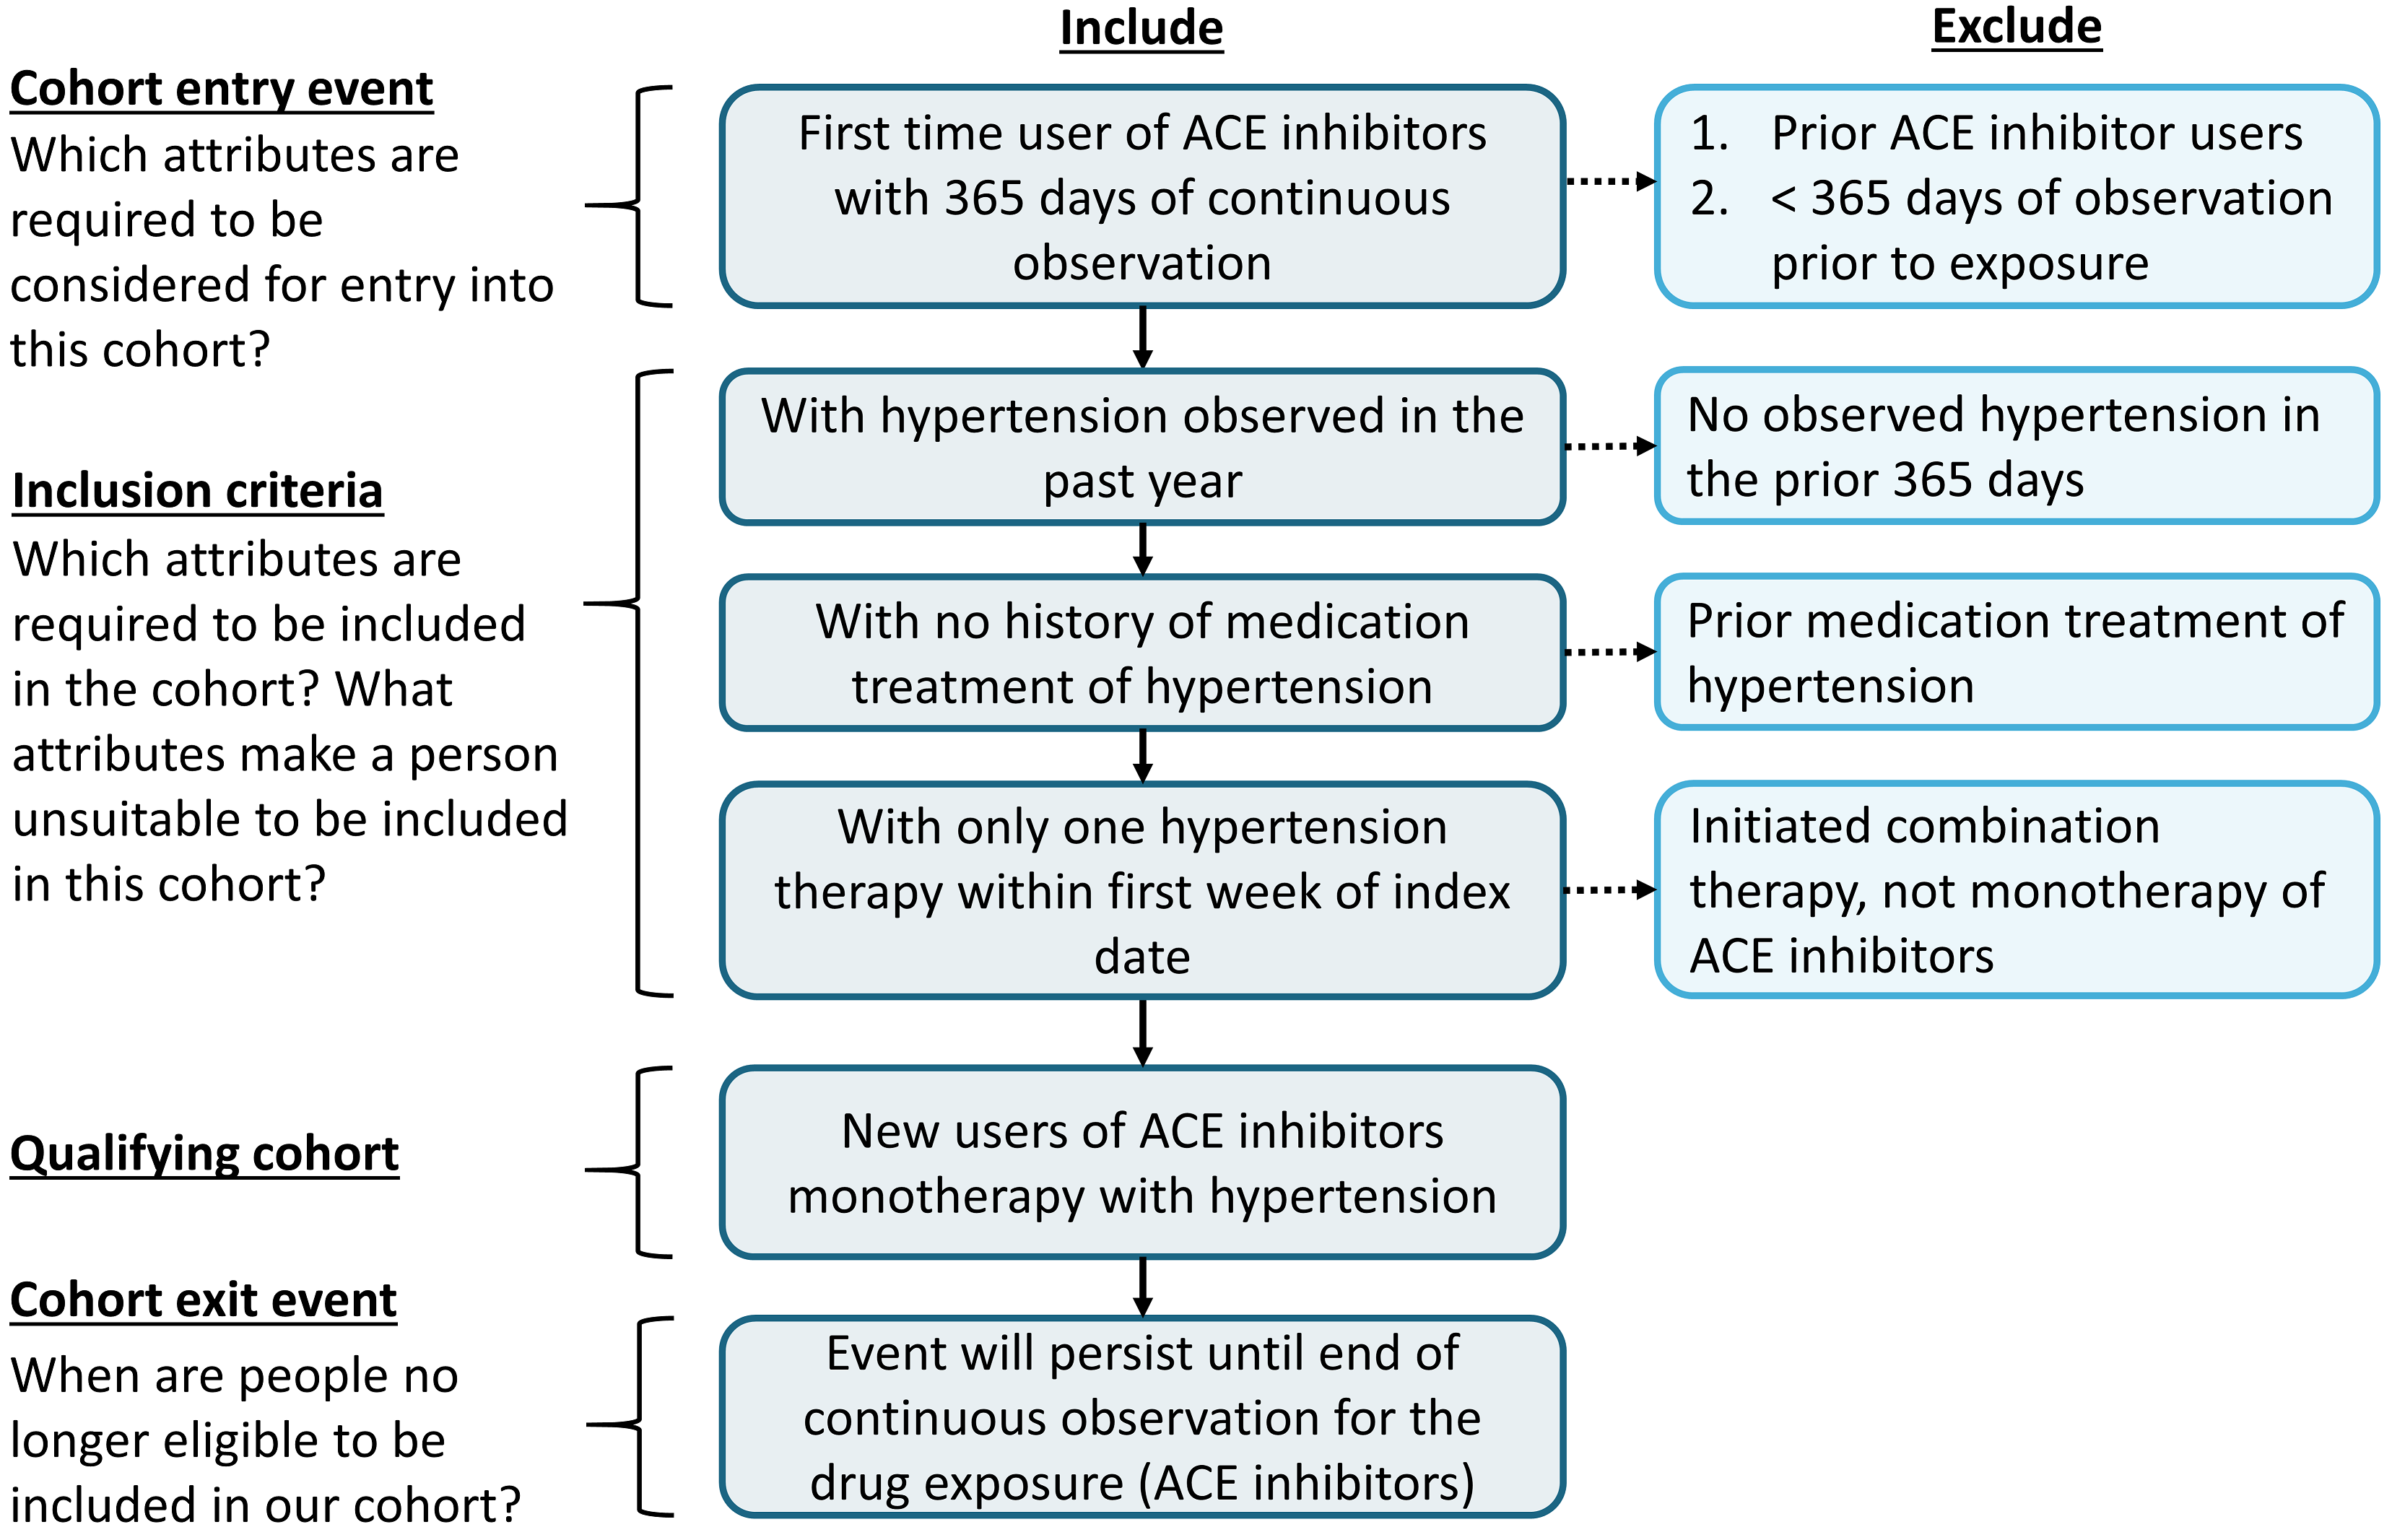
\includegraphics[width=1\linewidth]{images/Cohorts/CohortPractice} 

}

\caption{目標とするコホートの論理図}\label{fig:CohortPractice}
\end{figure}

コホートはATLASのユーザーインターフェースで作成することも、CDMに対して直接クエリを記述することもできます。この章では、これらの両方について簡単に説明します。

\section{ATLASを用いたコホートの実装}\label{atlasux3092ux7528ux3044ux305fux30b3ux30dbux30fcux30c8ux306eux5b9fux88c5}

まずATLASで始めるには、
\includegraphics{images/Cohorts/cohortdefinition.png}モジュールをクリックします。モジュールが読み込まれると、「New cohort」をクリックします。次の画面では空のコホート定義が表示されます。図\ref{fig:ATLASdefineacohort}に示す内容が画面に表示されます。

\begin{figure}

{\centering 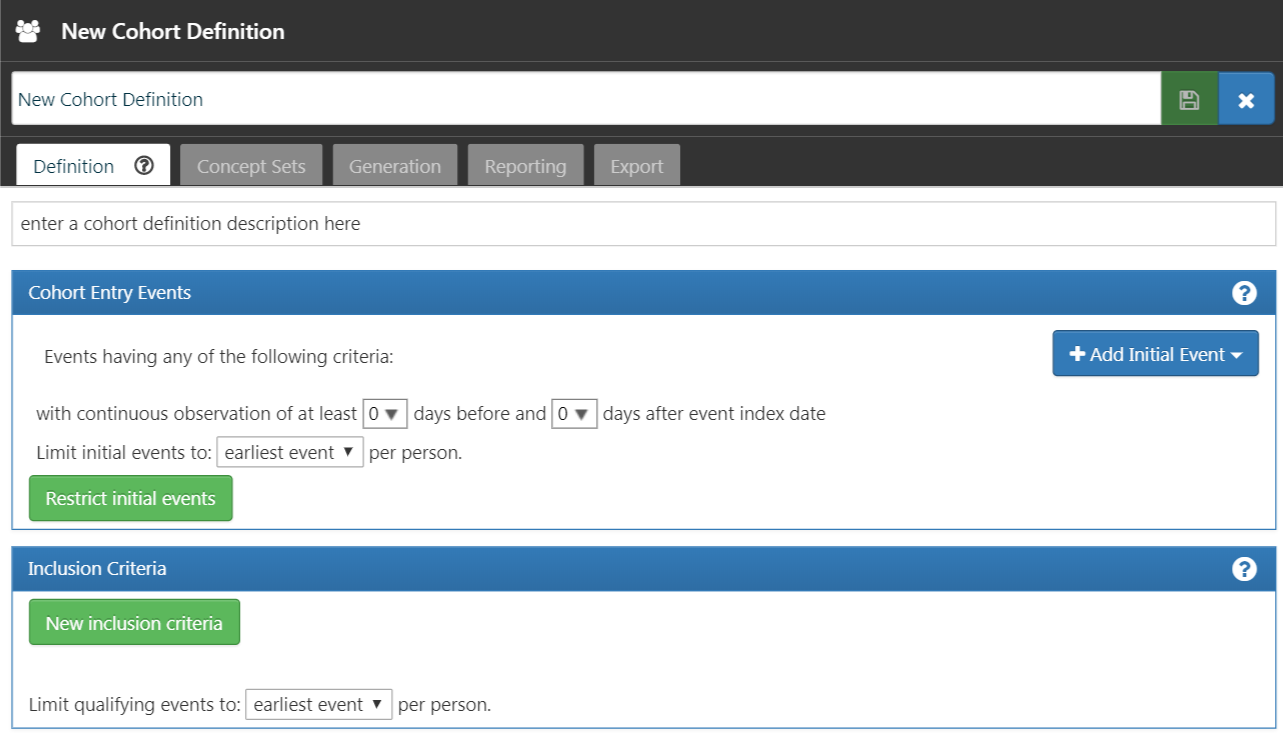
\includegraphics[width=1\linewidth]{images/Cohorts/ATLAS-defineacohort} 

}

\caption{新しいコホート定義}\label{fig:ATLASdefineacohort}
\end{figure}

まず最初に、「New Cohort Definition」からコホートの名前を自身のユニークな名前に変更することをお勧めします。「高血圧に対する第一選択単剤療法としてのACE阻害薬の新規ユーザー」のような名前を付けることができます。

\begin{rmdimportant}
ATLASは二つのコホートが全く同じ名前を持つことを許可しません。他のATLASコホートで既に使われている名前を選んだ場合、ATLASはポップアップエラーメッセージを表示します。
\end{rmdimportant}

名前を決めたら、
\includegraphics{images/Cohorts/save.png}をクリックしてコホートを保存します。

\subsection{初期イベント基準}\label{ux521dux671fux30a4ux30d9ux30f3ux30c8ux57faux6e96}

では、初期コホートイベントの定義を進めます。「Add initial event」をクリックします。どのドメインに基づいて基準を設定するかを選ばなければなりません。「どのドメインが初期コホートイベントかどうかをどのように知るのか?」という疑問を抱くかも知れません。これを解決しましょう。

\begin{figure}

{\centering 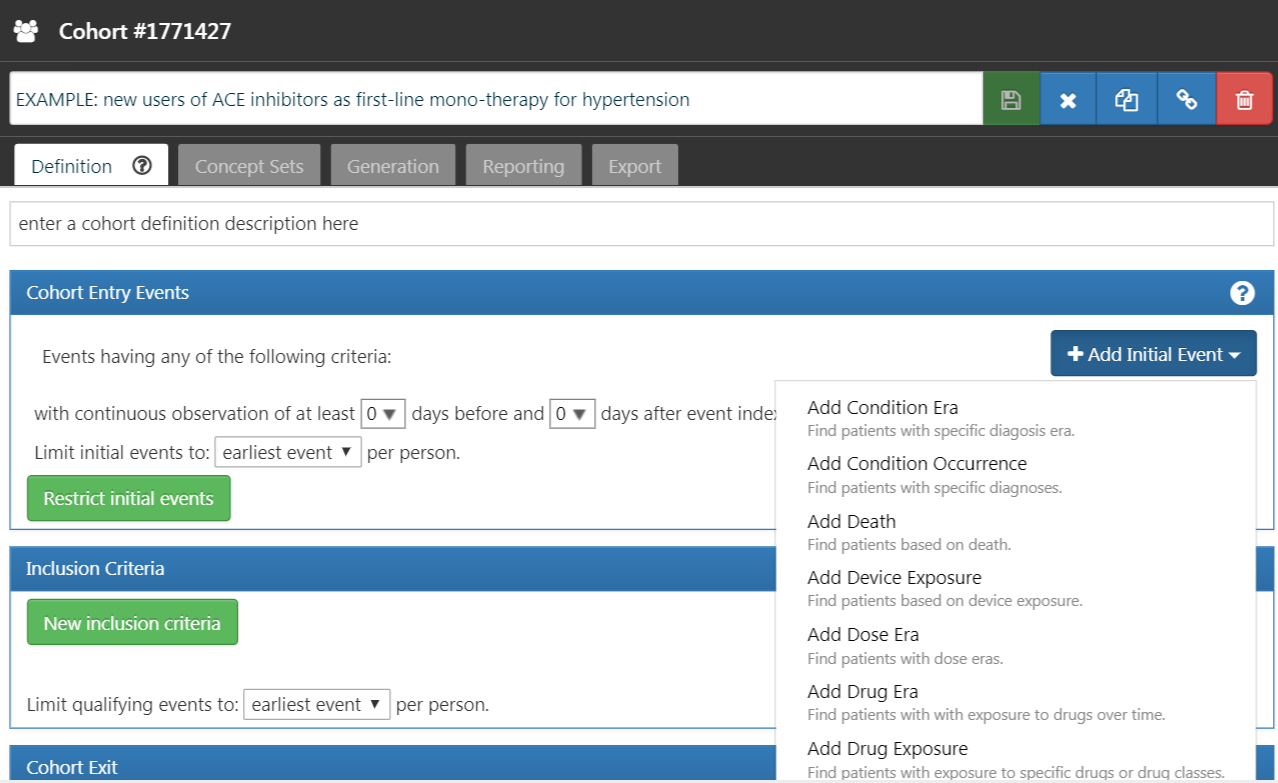
\includegraphics[width=1\linewidth]{images/Cohorts/ATLAS-initialevent} 

}

\caption{初期イベントの追加}\label{fig:ATLASinitialevent}
\end{figure}

図\ref{fig:ATLASinitialevent}に示されているように、ATLASは各基準の説明を提供しています。もしCONDITION\_OCCURRENCEに基づいた基準を構築している場合、特定の診断を持つ患者を探しているということになります。DRUG\_EXPOSUREに基づいた基準を構築している場合、特定の薬または薬クラスを持つ患者を探しているということになります。高血圧に対する第一選択治療としてACE阻害薬単剤療法を開始する患者を見つけるため、DRUG\_EXPOSURE基準を選択します。あなたが「しかし、高血圧としての診断も重要では?」と思うかも知れません。それは正しいです。高血圧は我々が構築する他の基準です。しかし、コホートの開始日はACE阻害薬治療の開始によって定義されるため、それが初期イベントです。高血圧の診断は、\emph{追加の資格基準}と呼ばれるものです。この基準を構築した後で再度考慮します。「Add Drug Exposure」をクリックします。

画面は選択した基準を表示するように更新されますが、まだ終了ではありません。図\ref{fig:ATLASdrugexposure}を参照すると、ATLASはどの薬を探しているのかを知りません。ATLASにACE阻害薬に関連するコンセプトセットを知らせる必要があります。

\begin{figure}

{\centering 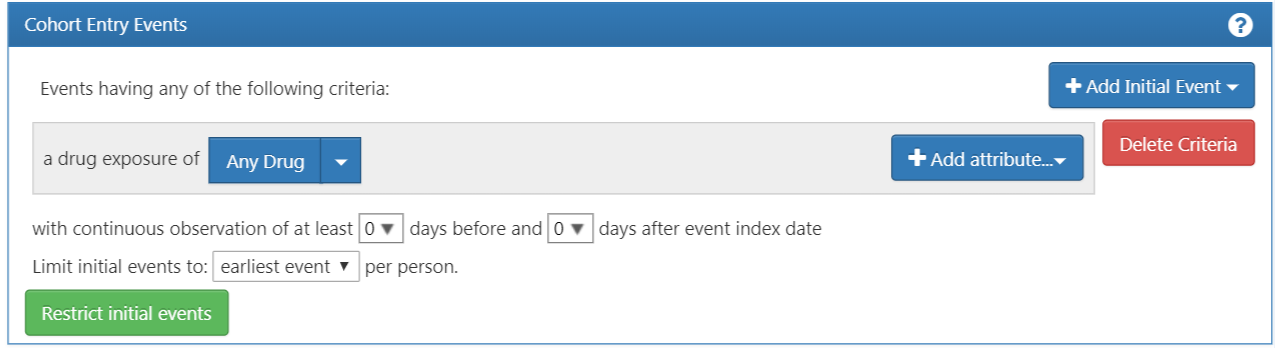
\includegraphics[width=1\linewidth]{images/Cohorts/ATLAS-drugexposure} 

}

\caption{薬剤曝露の定義}\label{fig:ATLASdrugexposure}
\end{figure}

\subsection{コンセプトセットの定義}\label{ux30b3ux30f3ux30bbux30d7ux30c8ux30bbux30c3ux30c8ux306eux5b9aux7fa9}

コンセプトセットを定義するためには、
\includegraphics{images/Cohorts/downarrow.png}をクリックして、ACE阻害薬を定義するためのコンセプトセットを取得するダイアログボックスを開きます。

\subsubsection*{シナリオ1: コンセプトセットを構築していない場合}\label{ux30b7ux30caux30eaux30aa1-ux30b3ux30f3ux30bbux30d7ux30c8ux30bbux30c3ux30c8ux3092ux69cbux7bc9ux3057ux3066ux3044ux306aux3044ux5834ux5408}
\addcontentsline{toc}{subsubsection}{シナリオ1: コンセプトセットを構築していない場合}

基準に適用するためのコンセプトセットを集めていない場合は、先にそれを行う必要があります。コホート定義内で「Concept set」タブに移動し、「New Concept Set」をクリックしてコンセプトセットを構築することができます。「Unnamed Concept Set」から任意の名前に変更する必要があります。そこから、
\includegraphics{images/Cohorts/search-2.png}モジュールを使用してACE阻害薬を表す臨床コンセプトを検索できます(図\ref{fig:aceinhibitors}を参照)。

\begin{figure}

{\centering 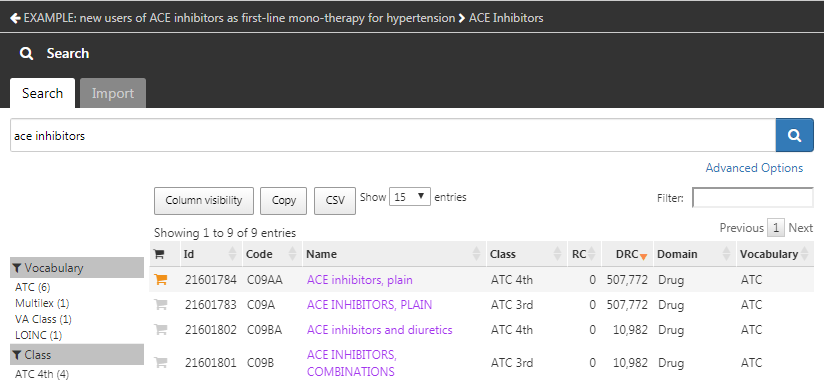
\includegraphics[width=1\linewidth]{images/Cohorts/aceinhibitors} 

}

\caption{語彙の検索 - ACE阻害薬}\label{fig:aceinhibitors}
\end{figure}

使用したい用語を見つけたら、
\includegraphics{images/Cohorts/shoppingcart.png}をクリックしてコンセプトを選択します。図\ref{fig:aceinhibitors}の左矢印を使用してコホート定義に戻ります。興味のある臨床コンセプトを見つけるための語彙のナビゲートは、チャプター\ref{StandardizedVocabularies}(標準化された語彙)に参照できます。

図\ref{fig:aceConceptSetExpression}は私たちのコンセプトセット表現を示しています。興味のあるすべてのACE阻害薬成分を選び、その子孫すべてを含め、これらの成分を含むすべての薬を含めています。「含まれているコンセプト」をクリックして、この表現に含まれている21,536のコンセプトすべてを確認することができ、「含まれているソースコード」をクリックして様々なコーディングシステムに含まれているすべてのソースコードを調査できます。

\begin{figure}

{\centering 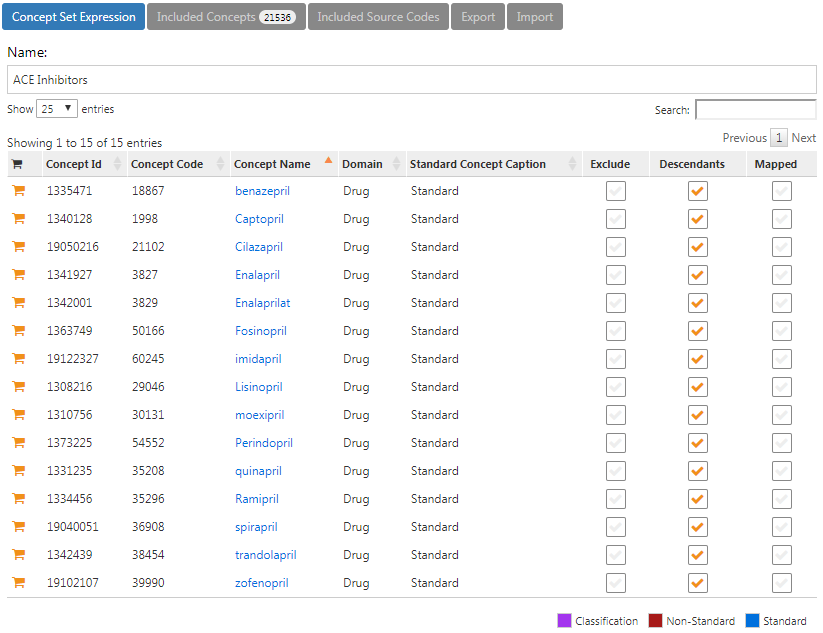
\includegraphics[width=1\linewidth]{images/Cohorts/aceConceptSetExpression} 

}

\caption{ACE阻害薬を含むコンセプトセット。}\label{fig:aceConceptSetExpression}
\end{figure}

\subsubsection*{シナリオ2: すでにコンセプトセットを構築している場合}\label{ux30b7ux30caux30eaux30aa2-ux3059ux3067ux306bux30b3ux30f3ux30bbux30d7ux30c8ux30bbux30c3ux30c8ux3092ux69cbux7bc9ux3057ux3066ux3044ux308bux5834ux5408}
\addcontentsline{toc}{subsubsection}{シナリオ2: すでにコンセプトセットを構築している場合}

すでにコンセプトセットを作成してATLASに保存している場合、「Import Concept Set」をクリックします。ダイアログボックスが開き、ATLASのコンセプトセットリポジトリからコンセプトを見つけるように促されます(図\ref{fig:ATLASfindyourconcept}を参照)。例の図ではユーザーはATLASに保存されているコンセプトセットを取得しています。右側の検索に「ace inhibitors」と入力し、コンセプトセットのリストを同じ名前を持つコンセプトのみに短縮しました。そこからユーザーはコンセプトセットの行をクリックして選択します。(注意: コンセプトセットを選択するとダイアログボックスは消えます。)選択したコンセプトセットの名前が「Any Drug」ボックスに更新されると、この操作が成功したことがわかります。

\begin{figure}

{\centering 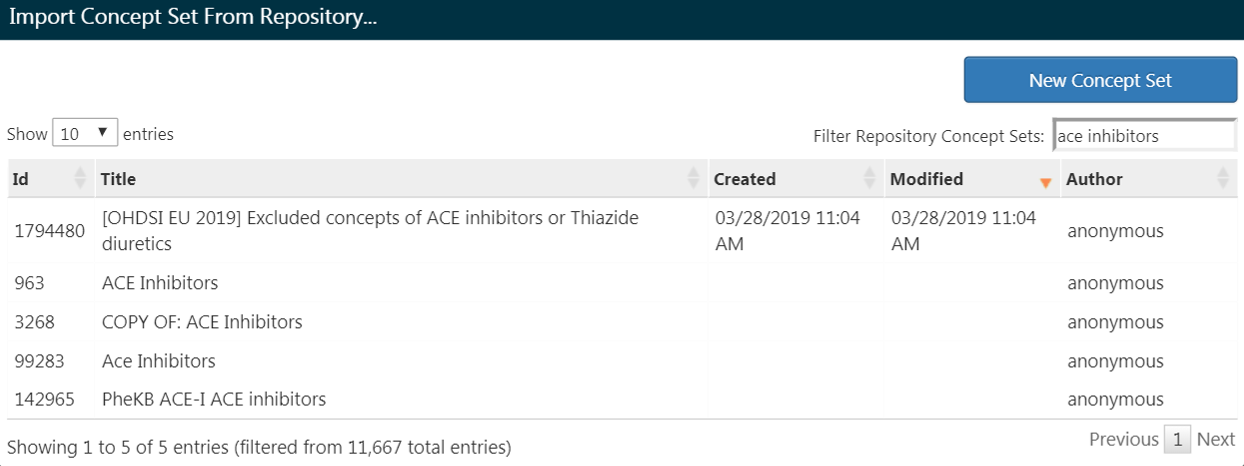
\includegraphics[width=1\linewidth]{images/Cohorts/ATLAS-findingyourconcept} 

}

\caption{ATLASリポジトリからのコンセプトセットのインポート}\label{fig:ATLASfindyourconcept}
\end{figure}

\subsection{追加の初期イベント基準}\label{ux8ffdux52a0ux306eux521dux671fux30a4ux30d9ux30f3ux30c8ux57faux6e96}

コンセプトセットを添付したら、まだ終了ではありません。質問は新たにACE阻害薬を初めて使用する患者を探すものです。これは、患者の記録において初めてのACE阻害薬曝露を表します。これを指定するには、「+Add attribute」をクリックします。次に「Add first exposure criteria」を選択します。注意:基準を構築する際に他の属性を指定することもできます。発生時の年齢、発生日、性別、薬剤に関連するその他の属性を指定できます。各ドメインの基準が異なることがあります。

選択したら、ウィンドウは自動的に閉じます。この追加属性は初期基準と同じボックスに表示されます(図\ref{fig:initialEventAce}を参照)。

\begin{rmdimportant}
現在のATLASのデザインは一部の人々を混乱させるかもしれません。見た目の通り、
\includegraphics{images/Cohorts/redX.png}は「No」を意味するものではありません。これは、基準を削除するための操作可能な機能です。もし
\includegraphics{images/Cohorts/redX.png}をクリックすると、この基準は消えます。したがって、基準を有効に保つには
\includegraphics{images/Cohorts/redX.png}を残す必要があります。
\end{rmdimportant}

これで初期の検証イベントが構築できました。初回の薬剤曝露をキャプチャするため、見落しがないことを知るために、ルックバックウィンドウを追加する必要があります。観察期間の短い患者が非表示の曝露を受ける場合があるため、観察期間の最低限度を強制することができます。これにより、記録の最初の発生をキャプチャしていることを確認するために、患者の履歴を見る最低期間を設定できます。この基準は他コホートでも異なる基準を選択することができます。365日間の継続的な観察を初期イベント前に要求します。観察期間を更新して、初期イベント後0日として更新します。最初のACE阻害薬の使用であることを保証するために、「earliest event」を選択します。図\ref{fig:initialEventAce}を参照してロジックを確認してください。

\begin{figure}

{\centering 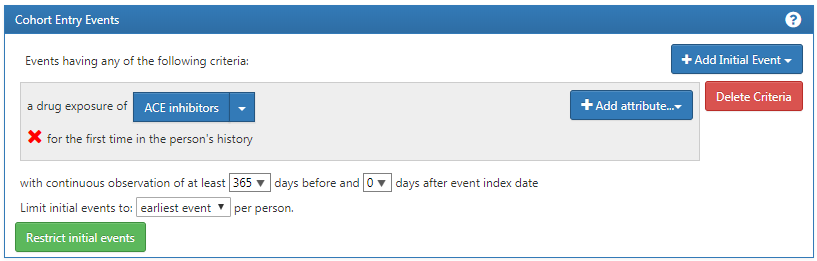
\includegraphics[width=1\linewidth]{images/Cohorts/initialEventAce} 

}

\caption{インデックス日付前に必要な継続的観察を設定する。}\label{fig:initialEventAce}
\end{figure}

このロジックがどのように組み合わさるかを説明すると、患者のタイムラインを組み立てることを考えることができます。

\begin{figure}

{\centering 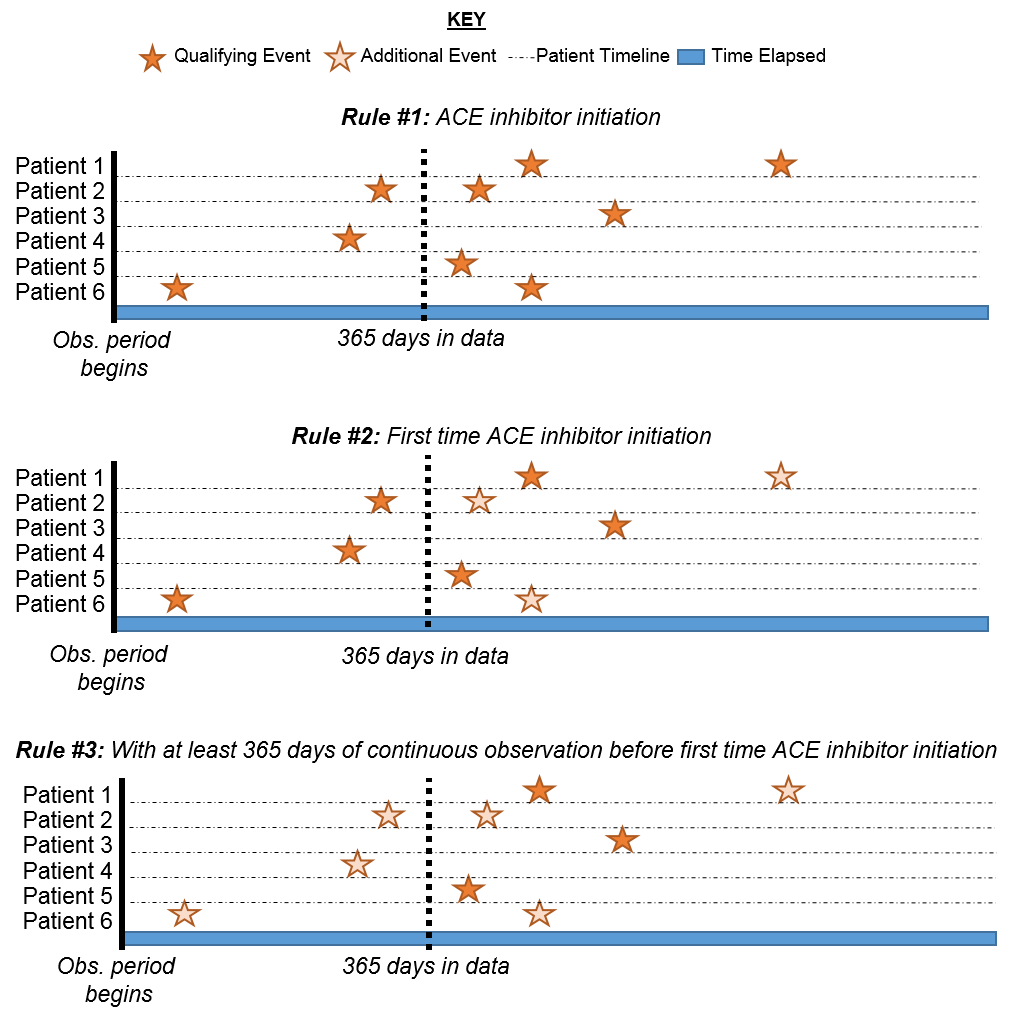
\includegraphics[width=1\linewidth]{images/Cohorts/EarliestEventExplained} 

}

\caption{基準の適用による患者の適格性の説明}\label{fig:EarliestEventExplained}
\end{figure}

図\ref{fig:EarliestEventExplained}では、各ラインがコホートに参加資格がある可能性のある単一の患者を表しています。塗りつぶされた星は、患者が指定された基準を満たすタイミングを表しています。追加の基準が適用されると、いくつかの星がより薄い色になります。これは、これらの患者が基準を満たす他の記録を持っていることを意味しますが、その基準を満たす前に他の記録があることを意味します。最終的な基準に達するまでに、私たちは初めてのACE阻害薬使用とその前の365日間の連続する観察を持つ患者の累積ビューを見ています。最初のイベントに限定することは冗長ですが、すべての選択で明確なロジックを維持することに役立ちます。独自のコホートを構築するときには、\href{http://forums.ohdsi.org}{OHDSIフォーラム}の研究者セクションに参加して、コホート論理の構築について第二の意見を得ることをお勧めします。

\subsection{包括基準}\label{ux5305ux62ecux57faux6e96}

コホートエントリエベントを指定したら、追加の資格イベントを「Restrict initial events」または「New inclusion criteria」のいずれかに追加することができます。これら二つのオプション間の基本的な違いは、ATLASが提供する中間情報の内容です。「Restrict initial events」に追加基準を加えると、ATLASでカウントを生成するときに、これらすべての基準を満たす人の数だけが返されます。「New inclusion criteria」に基準を追加すると、追加の包括基準を適用することによって失う患者数を示す削減チャートが表示されます。各ルールがコホート定義の全体的な成功に与える影響を理解するために、包括基準セクションを利用することを強くお勧めします。特定の包括基準がコホートに入る人の数を大幅に制限する可能性があることがわかります。この段階では、コホートを大きくするためにこの基準を緩和する選択をするかもしれません。最終的には、このコホートを組み立てる専門家の合意に従います。

コホートのメンバーシップに関するロジックをさらに追加するために「New inclusion criteria」をクリックしてください。このセクションの機能は、前述のコホート基準の構築方法と同じです。私たちの最初の追加基準は次のとおりです:\emph{ACE阻害薬の最初の開始日から365日から0日以内の少なくとも1回の高血圧障害の発生がある患者のみ}。新しい包括基準を追加するには「New inclusion criteria」をクリックします。基準に名前を付け、必要に応じて探している内容についての簡単な説明を書き込むことができます。これは自分が定義している基準を覚えるためのもので、コホートの整合性に影響を与えるものではありません。

新しい基準に注釈を付けたら、「+Add criteria to group」ボタンをクリックして、このルールの実際の基準を構築します。このボタンは「Add Initial Event」と同様に機能します。ただし、初期イベントを指定するわけではありません。複数の基準を追加できるため、「add criteria to group」と指定されています。たとえば、病気を見つけるための複数の方法(例:CONDITION\_OCCURRENCEのロジック、この状態の代理としてのDRUG\_EXPOSUREのロジック、この状態の代理としてのMEASUREMENTのロジック)があります。これらは別々のドメインであり、異なる基準を必要としますが、この状態を探すための1つの基準にグループ化できます。この場合、高血圧の診断を見つけるため「Add condition occurrence」を指定する。

\section{SQLを使用したコホートの実装}\label{sqlux3092ux4f7fux7528ux3057ux305fux30b3ux30dbux30fcux30c8ux306eux5b9fux88c5}

ここでは、SQLとRを使用して同じコホートを作成する方法について説明します。第\ref{SqlAndR}章で説明したように、OHDSIはSqlRenderとDatabaseConnectorという2つのRパッケージを提供しており、これらを組み合わせることで、多様なデータベースプラットフォームに対して自動的に翻訳・実行されるSQLコードを記述できます。

理解しやすさのために、SQLをいくつかのチャンクに分割し、各チャンクが次のチャンクで使用される一時テーブルを生成するようにします。これはおそらく最も計算効率の良い方法ではありませんが、非常に長い一つのステートメントよりも読みやすくなります。

\subsection{データベースへの接続}\label{ux30c7ux30fcux30bfux30d9ux30fcux30b9ux3078ux306eux63a5ux7d9a-1}

最初にRに対してサーバーへの接続方法を指示する必要があります。これには\href{https://ohdsi.github.io/DatabaseConnector/}{DatabaseConnector}パッケージを使用し、\texttt{createConnectionDetails}という名前の関数を提供します。各データベース管理システム(DBMS)に必要な具体的な設定については、\texttt{?createConnectionDetails}と入力してください。例えば、以下のコードでPostgreSQLデータベースに接続することができます:

\begin{Shaded}
\begin{Highlighting}[]
\FunctionTok{library}\NormalTok{(CohortMethod)}
\NormalTok{connDetails }\OtherTok{\textless{}{-}} \FunctionTok{createConnectionDetails}\NormalTok{(}\AttributeTok{dbms =} \StringTok{"postgresql"}\NormalTok{,}
                                       \AttributeTok{server =} \StringTok{"localhost/ohdsi"}\NormalTok{,}
                                       \AttributeTok{user =} \StringTok{"joe"}\NormalTok{,}
                                       \AttributeTok{password =} \StringTok{"supersecret"}\NormalTok{)}

\NormalTok{cdmDbSchema }\OtherTok{\textless{}{-}} \StringTok{"my\_cdm\_data"}
\NormalTok{cohortDbSchema }\OtherTok{\textless{}{-}} \StringTok{"scratch"}
\NormalTok{cohortTable }\OtherTok{\textless{}{-}} \StringTok{"my\_cohorts"}
\end{Highlighting}
\end{Shaded}

最後の3行で、\texttt{cdmDbSchema}、\texttt{cohortDbSchema}、および\texttt{cohortTable}の変数を定義しています。これらは後で、CDM形式のデータが存在する場所と、興味のあるコホートを作成する場所をRに伝えるために使用します。Microsoft SQL Serverの場合、データベースのスキーマはデータベースとスキーマの両方を指定する必要があることに注意してください。例:\texttt{cdmDbSchema\ \textless{}-\ "my\_cdm\_data.dbo"}。

\subsection{コンセプトの指定}\label{ux30b3ux30f3ux30bbux30d7ux30c8ux306eux6307ux5b9a}

読みやすさのために、必要なコンセプトIDをRで定義し、それらをSQLに渡します:

\begin{Shaded}
\begin{Highlighting}[]
\NormalTok{aceI }\OtherTok{\textless{}{-}} \FunctionTok{c}\NormalTok{(}\DecValTok{1308216}\NormalTok{, }\DecValTok{1310756}\NormalTok{, }\DecValTok{1331235}\NormalTok{, }\DecValTok{1334456}\NormalTok{, }\DecValTok{1335471}\NormalTok{, }\DecValTok{1340128}\NormalTok{, }\DecValTok{1341927}\NormalTok{,}
          \DecValTok{1342439}\NormalTok{, }\DecValTok{1363749}\NormalTok{, }\DecValTok{1373225}\NormalTok{)}

\NormalTok{hypertension }\OtherTok{\textless{}{-}} \DecValTok{316866}

\NormalTok{allHtDrugs }\OtherTok{\textless{}{-}} \FunctionTok{c}\NormalTok{(}\DecValTok{904542}\NormalTok{, }\DecValTok{907013}\NormalTok{, }\DecValTok{932745}\NormalTok{, }\DecValTok{942350}\NormalTok{, }\DecValTok{956874}\NormalTok{, }\DecValTok{970250}\NormalTok{, }\DecValTok{974166}\NormalTok{,}
                  \DecValTok{978555}\NormalTok{, }\DecValTok{991382}\NormalTok{, }\DecValTok{1305447}\NormalTok{, }\DecValTok{1307046}\NormalTok{, }\DecValTok{1307863}\NormalTok{, }\DecValTok{1308216}\NormalTok{,}
                  \DecValTok{1308842}\NormalTok{, }\DecValTok{1309068}\NormalTok{, }\DecValTok{1309799}\NormalTok{, }\DecValTok{1310756}\NormalTok{, }\DecValTok{1313200}\NormalTok{, }\DecValTok{1314002}\NormalTok{,}
                  \DecValTok{1314577}\NormalTok{, }\DecValTok{1317640}\NormalTok{, }\DecValTok{1317967}\NormalTok{, }\DecValTok{1318137}\NormalTok{, }\DecValTok{1318853}\NormalTok{, }\DecValTok{1319880}\NormalTok{,}
                  \DecValTok{1319998}\NormalTok{, }\DecValTok{1322081}\NormalTok{, }\DecValTok{1326012}\NormalTok{, }\DecValTok{1327978}\NormalTok{, }\DecValTok{1328165}\NormalTok{, }\DecValTok{1331235}\NormalTok{,}
                  \DecValTok{1332418}\NormalTok{, }\DecValTok{1334456}\NormalTok{, }\DecValTok{1335471}\NormalTok{, }\DecValTok{1338005}\NormalTok{, }\DecValTok{1340128}\NormalTok{, }\DecValTok{1341238}\NormalTok{,}
                  \DecValTok{1341927}\NormalTok{, }\DecValTok{1342439}\NormalTok{, }\DecValTok{1344965}\NormalTok{, }\DecValTok{1345858}\NormalTok{, }\DecValTok{1346686}\NormalTok{, }\DecValTok{1346823}\NormalTok{,}
                  \DecValTok{1347384}\NormalTok{, }\DecValTok{1350489}\NormalTok{, }\DecValTok{1351557}\NormalTok{, }\DecValTok{1353766}\NormalTok{, }\DecValTok{1353776}\NormalTok{, }\DecValTok{1363053}\NormalTok{,}
                  \DecValTok{1363749}\NormalTok{, }\DecValTok{1367500}\NormalTok{, }\DecValTok{1373225}\NormalTok{, }\DecValTok{1373928}\NormalTok{, }\DecValTok{1386957}\NormalTok{, }\DecValTok{1395058}\NormalTok{,}
                  \DecValTok{1398937}\NormalTok{, }\DecValTok{40226742}\NormalTok{, }\DecValTok{40235485}\NormalTok{)}
\end{Highlighting}
\end{Shaded}

\subsection{初回使用の発見}\label{ux521dux56deux4f7fux7528ux306eux767aux898b}

まず、各患者のACE阻害薬の初回使用を見つけます:

\begin{Shaded}
\begin{Highlighting}[]
\NormalTok{conn }\OtherTok{\textless{}{-}} \FunctionTok{connect}\NormalTok{(connDetails)}

\NormalTok{sql }\OtherTok{\textless{}{-}} \StringTok{"SELECT person\_id AS subject\_id,}
\StringTok{  MIN(drug\_exposure\_start\_date) AS cohort\_start\_date}
\StringTok{INTO \#first\_use}
\StringTok{FROM @cdm\_db\_schema.drug\_exposure}
\StringTok{INNER JOIN @cdm\_db\_schema.concept\_ancestor}
\StringTok{  ON descendant\_concept\_id = drug\_concept\_id}
\StringTok{WHERE ancestor\_concept\_id IN (@ace\_i)}
\StringTok{GROUP BY person\_id;"}

\FunctionTok{renderTranslateExecuteSql}\NormalTok{(conn,}
\NormalTok{                          sql,}
                          \AttributeTok{cdm\_db\_schema =}\NormalTok{ cdmDbSchema,}
                          \AttributeTok{ace\_i =}\NormalTok{ aceI)}
\end{Highlighting}
\end{Shaded}

DRUG\_EXPOSUREテーブルをCONCEPT\_ANCESTORテーブルと結合することで、ACE阻害薬を含むすべての薬を見つけていることに注意してください。

\subsection{365日の事前観察が必要}\label{ux65e5ux306eux4e8bux524dux89b3ux5bdfux304cux5fc5ux8981}

次に、OBSERVATION\_PERIODテーブルと結合して365日間の連続した事前の観察が必要です:

\begin{Shaded}
\begin{Highlighting}[]
\NormalTok{sql }\OtherTok{\textless{}{-}} \StringTok{"SELECT subject\_id,}
\StringTok{  cohort\_start\_date}
\StringTok{INTO \#has\_prior\_obs}
\StringTok{FROM \#first\_use}
\StringTok{INNER JOIN @cdm\_db\_schema.observation\_period}
\StringTok{  ON subject\_id = person\_id}
\StringTok{    AND observation\_period\_start\_date \textless{}= cohort\_start\_date}
\StringTok{    AND observation\_period\_end\_date \textgreater{}= cohort\_start\_date}
\StringTok{WHERE DATEADD(DAY, 365, observation\_period\_start\_date) \textless{} cohort\_start\_date;"}

\FunctionTok{renderTranslateExecuteSql}\NormalTok{(conn, sql, }\AttributeTok{cdm\_db\_schema =}\NormalTok{ cdmDbSchema)}
\end{Highlighting}
\end{Shaded}

\subsection{高血圧の前診断が必要}\label{ux9ad8ux8840ux5727ux306eux524dux8a3aux65adux304cux5fc5ux8981}

365日前に高血圧の診断が必要です:

\begin{Shaded}
\begin{Highlighting}[]
\NormalTok{sql }\OtherTok{\textless{}{-}} \StringTok{"SELECT DISTINCT subject\_id,}
\StringTok{  cohort\_start\_date}
\StringTok{INTO \#has\_ht}
\StringTok{FROM \#has\_prior\_obs}
\StringTok{INNER JOIN @cdm\_db\_schema.condition\_occurrence}
\StringTok{  ON subject\_id = person\_id}
\StringTok{    AND condition\_start\_date \textless{}= cohort\_start\_date}
\StringTok{    AND condition\_start\_date \textgreater{}= DATEADD(DAY, {-}365, cohort\_start\_date)}
\StringTok{INNER JOIN @cdm\_db\_schema.concept\_ancestor}
\StringTok{  ON descendant\_concept\_id = condition\_concept\_id}
\StringTok{WHERE ancestor\_concept\_id = @hypertension;"}

\FunctionTok{renderTranslateExecuteSql}\NormalTok{(conn,}
\NormalTok{                          sql,}
                          \AttributeTok{cdm\_db\_schema =}\NormalTok{ cdmDbSchema,}
                          \AttributeTok{hypertension =}\NormalTok{ hypertension)}
\end{Highlighting}
\end{Shaded}

過去に複数の高血圧診断がある場合でも、重複するコホートエントリーを作成しないように\texttt{SELECT\ DISTINCT}を使用していることに注意してください。

\subsection{治療の無前使用が必要}\label{ux6cbbux7642ux306eux7121ux524dux4f7fux7528ux304cux5fc5ux8981}

高血圧治療の前使用がないことが必要です:

\begin{Shaded}
\begin{Highlighting}[]
\NormalTok{sql }\OtherTok{\textless{}{-}} \StringTok{"SELECT subject\_id,}
\StringTok{  cohort\_start\_date}
\StringTok{INTO \#no\_prior\_ht\_drugs}
\StringTok{FROM \#has\_ht}
\StringTok{LEFT JOIN (}
\StringTok{  SELECT *}
\StringTok{  FROM @cdm\_db\_schema.drug\_exposure}
\StringTok{  INNER JOIN @cdm\_db\_schema.concept\_ancestor}
\StringTok{    ON descendant\_concept\_id = drug\_concept\_id}
\StringTok{  WHERE ancestor\_concept\_id IN (@all\_ht\_drugs)}
\StringTok{) ht\_drugs}
\StringTok{  ON subject\_id = person\_id}
\StringTok{    AND drug\_exposure\_start\_date \textless{} cohort\_start\_date}
\StringTok{WHERE person\_id IS NULL;"}

\FunctionTok{renderTranslateExecuteSql}\NormalTok{(conn,}
\NormalTok{                          sql,}
                          \AttributeTok{cdm\_db\_schema =}\NormalTok{ cdmDbSchema,}
                          \AttributeTok{all\_ht\_drugs =}\NormalTok{ allHtDrugs)}
\end{Highlighting}
\end{Shaded}

LEFT JOINを使用しており、DRUG\_EXPOSUREテーブルからのperson\_idがNULLの場合のみ行を許可することに注意してください。

\subsection{単剤療法}\label{ux5358ux5264ux7642ux6cd5}

コホートエントリーの最初の7日間に高血圧治療への一回のみの曝露が必要です:

\begin{Shaded}
\begin{Highlighting}[]
\NormalTok{sql }\OtherTok{\textless{}{-}} \StringTok{"SELECT subject\_id,}
\StringTok{  cohort\_start\_date}
\StringTok{INTO \#monotherapy}
\StringTok{FROM \#no\_prior\_ht\_drugs}
\StringTok{INNER JOIN @cdm\_db\_schema.drug\_exposure}
\StringTok{  ON subject\_id = person\_id}
\StringTok{    AND drug\_exposure\_start\_date \textgreater{}= cohort\_start\_date}
\StringTok{    AND drug\_exposure\_start\_date \textless{}= DATEADD(DAY, 7, cohort\_start\_date)}
\StringTok{INNER JOIN @cdm\_db\_schema.concept\_ancestor}
\StringTok{  ON descendant\_concept\_id = drug\_concept\_id}
\StringTok{WHERE ancestor\_concept\_id IN (@all\_ht\_drugs)}
\StringTok{GROUP BY subject\_id,}
\StringTok{  cohort\_start\_date}
\StringTok{HAVING COUNT(*) = 1;"}

\FunctionTok{renderTranslateExecuteSql}\NormalTok{(conn,}
\NormalTok{                          sql,}
                          \AttributeTok{cdm\_db\_schema =}\NormalTok{ cdmDbSchema,}
                          \AttributeTok{all\_ht\_drugs =}\NormalTok{ allHtDrugs)}
\end{Highlighting}
\end{Shaded}

\subsection{コホートの終了}\label{ux30b3ux30dbux30fcux30c8ux306eux7d42ux4e86}

これでコホートは完全に指定されましたが、コホートの終了日を除きます。コホートは曝露が停止した時点で終了し、次の曝露の間に最大で30日のギャップを許容します。これは、最初の薬剤曝露だけでなく、それに続くACE阻害薬の曝露も考慮する必要があることを意味します。連続する曝露を統合するためのSQLは非常に複雑になることがあります。幸いなことに、連続する曝露を効率的に作成する標準コードが定義されています(このコードはクリス・ノールによって書かれ、OHDSI内では「魔法」と呼ばれることがよくあります)。まず、統合したいすべての曝露を含む一時テーブルを作成します:

\begin{Shaded}
\begin{Highlighting}[]
\NormalTok{sql }\OtherTok{\textless{}{-}} \StringTok{"}
\StringTok{  SELECT person\_id,}
\StringTok{    CAST(1 AS INT) AS concept\_id,}
\StringTok{    drug\_exposure\_start\_date AS exposure\_start\_date,}
\StringTok{    drug\_exposure\_end\_date AS exposure\_end\_date}
\StringTok{  INTO \#exposure}
\StringTok{  FROM @cdm\_db\_schema.drug\_exposure}
\StringTok{  INNER JOIN @cdm\_db\_schema.concept\_ancestor}
\StringTok{    ON descendant\_concept\_id = drug\_concept\_id}
\StringTok{  WHERE ancestor\_concept\_id IN (@ace\_i);"}
\FunctionTok{renderTranslateExecuteSql}\NormalTok{(conn,}
\NormalTok{                          sql,}
                          \AttributeTok{cdm\_db\_schema =}\NormalTok{ cdmDbSchema,}
                          \AttributeTok{ace\_i =}\NormalTok{ aceI)}
\end{Highlighting}
\end{Shaded}

次に、連続する曝露を統合するための標準コードを実行します:

\begin{Shaded}
\begin{Highlighting}[]
\NormalTok{sql }\OtherTok{\textless{}{-}} \StringTok{"}
\StringTok{SELECT ends.person\_id AS subject\_id,}
\StringTok{    ends.concept\_id AS cohort\_definition\_id,}
\StringTok{  MIN(exposure\_start\_date) AS cohort\_start\_date,}
\StringTok{  ends.era\_end\_date AS cohort\_end\_date}
\StringTok{INTO \#exposure\_era}
\StringTok{FROM (}
\StringTok{  SELECT exposure.person\_id,}
\StringTok{    exposure.concept\_id,}
\StringTok{    exposure.exposure\_start\_date,}
\StringTok{    MIN(events.end\_date) AS era\_end\_date}
\StringTok{  FROM \#exposure exposure}
\StringTok{  JOIN (}
\StringTok{{-}{-}cteEndDates}
\StringTok{    SELECT person\_id,}
\StringTok{      concept\_id,}
\StringTok{      DATEADD(DAY, {-} 1 * @max\_gap, event\_date) AS end\_date}
\StringTok{    FROM (}
\StringTok{      SELECT person\_id,}
\StringTok{        concept\_id,}
\StringTok{        event\_date,}
\StringTok{        event\_type,}
\StringTok{        MAX(start\_ordinal) OVER (}
\StringTok{          PARTITION BY person\_id ,concept\_id ORDER BY event\_date,}
\StringTok{              event\_type ROWS UNBOUNDED PRECEDING}
\StringTok{          ) AS start\_ordinal,}
\StringTok{        ROW\_NUMBER() OVER (}
\StringTok{          PARTITION BY person\_id, concept\_id ORDER BY event\_date,}
\StringTok{            event\_type}
\StringTok{          ) AS overall\_ord}
\StringTok{      FROM (}
\StringTok{{-}{-} select the start dates, assigning a row number to each}
\StringTok{        SELECT person\_id,}
\StringTok{          concept\_id,}
\StringTok{          exposure\_start\_date AS event\_date,}
\StringTok{          0 AS event\_type,}
\StringTok{          ROW\_NUMBER() OVER (}
\StringTok{            PARTITION BY person\_id, concept\_id ORDER BY exposure\_start\_date}
\StringTok{            ) AS start\_ordinal}
\StringTok{        FROM \#exposure exposure}

\StringTok{        UNION ALL}
\StringTok{{-}{-} add the end dates with NULL as the row number, padding the end dates by}
\StringTok{{-}{-} @max\_gap to allow a grace period for overlapping ranges.}

\StringTok{        SELECT person\_id,}
\StringTok{          concept\_id,}
\StringTok{          DATEADD(day, @max\_gap, exposure\_end\_date),}
\StringTok{          1 AS event\_type,}
\StringTok{          NULL}
\StringTok{        FROM \#exposure exposure}
\StringTok{        ) rawdata}
\StringTok{    ) events}
\StringTok{  WHERE 2 * events.start\_ordinal {-} events.overall\_ord = 0}
\StringTok{  ) events}
\StringTok{  ON exposure.person\_id = events.person\_id}
\StringTok{      AND exposure.concept\_id = events.concept\_id}
\StringTok{      AND events.end\_date \textgreater{}= exposure.exposure\_end\_date}
\StringTok{  GROUP BY exposure.person\_id,}
\StringTok{      exposure.concept\_id,}
\StringTok{      exposure.exposure\_start\_date}
\StringTok{  ) ends}
\StringTok{GROUP BY ends.person\_id,}
\StringTok{  concept\_id,}
\StringTok{  ends.era\_end\_date;"}

\FunctionTok{renderTranslateExecuteSql}\NormalTok{(conn,}
\NormalTok{                          sql,}
                          \AttributeTok{cdm\_db\_schema =}\NormalTok{ cdmDbSchema,}
                          \AttributeTok{max\_gap =} \DecValTok{30}\NormalTok{)}
\end{Highlighting}
\end{Shaded}

このコードは、曝露間のギャップを\texttt{max\_gap}引数で定義しながら、すべての連続する曝露を統合します。結果として得られた薬剤曝露の期間は、\texttt{\#exposure\_era}と呼ばれる一時テーブルに書き込まれます。

次に、これらのACE阻害薬の曝露期間を元のコホートに結合し、期間終了日をコホートの終了日として使用します:

\begin{Shaded}
\begin{Highlighting}[]
\NormalTok{sql }\OtherTok{\textless{}{-}} \StringTok{"SELECT ee.subject\_id,}
\StringTok{  CAST(1 AS INT) AS cohort\_definition\_id,}
\StringTok{  ee.cohort\_start\_date,}
\StringTok{  ee.cohort\_end\_date}
\StringTok{INTO @cohort\_db\_schema.@cohort\_table}
\StringTok{FROM \#monotherapy mt}
\StringTok{INNER JOIN \#exposure\_era ee}
\StringTok{  ON mt.subject\_id = ee.subject\_id}
\StringTok{    AND mt.cohort\_start\_date = ee.cohort\_start\_date;"}

\FunctionTok{renderTranslateExecuteSql}\NormalTok{(conn,}
\NormalTok{                          sql,}
                          \AttributeTok{cohort\_db\_schema =}\NormalTok{ cohortDbSchema,}
                          \AttributeTok{cohort\_table =}\NormalTok{ cohortTable)}
\end{Highlighting}
\end{Shaded}

ここで、以前に定義したスキーマとテーブルに最終的なコホートを保存します。他のコホートと区別するために1のコホート定義IDを割り当てます。

\subsection{クリーンアップ}\label{ux30afux30eaux30fcux30f3ux30a2ux30c3ux30d7-1}

最後に、作成した一時テーブルをすべてクリーンアップし、データベースサーバーから切断することをお勧めします:

\begin{Shaded}
\begin{Highlighting}[]
\NormalTok{sql }\OtherTok{\textless{}{-}} \StringTok{"TRUNCATE TABLE \#first\_use;}
\StringTok{DROP TABLE \#first\_use;}

\StringTok{TRUNCATE TABLE \#has\_prior\_obs;}
\StringTok{DROP TABLE \#has\_prior\_obs;}

\StringTok{TRUNCATE TABLE \#has\_ht;}
\StringTok{DROP TABLE \#has\_ht;}

\StringTok{TRUNCATE TABLE \#no\_prior\_ht\_drugs;}
\StringTok{DROP TABLE \#no\_prior\_ht\_drugs;}

\StringTok{TRUNCATE TABLE \#monotherapy;}
\StringTok{DROP TABLE \#monotherapy;}

\StringTok{TRUNCATE TABLE \#exposure;}
\StringTok{DROP TABLE \#exposure;}

\StringTok{TRUNCATE TABLE \#exposure\_era;}
\StringTok{DROP TABLE \#exposure\_era;"}

\FunctionTok{renderTranslateExecuteSql}\NormalTok{(conn, sql)}

\FunctionTok{disconnect}\NormalTok{(conn)}
\end{Highlighting}
\end{Shaded}

\section{サマリー}\label{ux30b5ux30deux30eaux30fc}

\begin{rmdsummary}
\begin{itemize}
\item
  コホートとは、1つまたは複数の選択基準を満たす人々の集合である。
\item
  コホート定義とは、特定のコホートを識別するために使用されるロジックの説明である。
\item
  コホートは、関心のある曝露やアウトカムを定義するために、OHDSIアナリティクスツール全体で使用(再利用)される。
\item
  コホートを構築するための2つの主要なアプローチがある:ルールベースと確率論的アプローチ。
\item
  ルールベースのコホート定義は、ATLASまたはSQLを使用して作成できる。
\end{itemize}
\end{rmdsummary}

\section{演習}\label{ux6f14ux7fd2-3}

\subsubsection*{前提条件}\label{ux524dux63d0ux6761ux4ef6-4}
\addcontentsline{toc}{subsubsection}{前提条件}

最初の演習のためには、ATLASインスタンスへのアクセスが必要である。以下のインスタンス \url{http://atlas-demo.ohdsi.org} またはアクセス可能な他のインスタンスを使用することができる。

\begin{exercise}
\protect\hypertarget{exr:exerciseCohortsAtlas}{}\label{exr:exerciseCohortsAtlas}

以下の基準に従ってATLASでコホート定義を作成せよ:

\begin{itemize}
\tightlist
\item
  ジクロフェナクの新規ユーザー
\item
  16歳以上
\item
  曝露前に少なくとも365日の継続的な観察期間があること
\item
  以前にNSAID(非ステロイド性抗炎症薬)への曝露がないこと
\item
  以前に癌の診断がないこと
\item
  コホート終了を曝露の中断(30日間のギャップを許容)として定義すること
\end{itemize}

\end{exercise}

\subsubsection*{前提条件}\label{ux524dux63d0ux6761ux4ef6-5}
\addcontentsline{toc}{subsubsection}{前提条件}

第二の演習では、R、R-StudioおよびJavaがインストールされていることを前提とする。セクション \ref{installR}で説明されている。また、\href{https://ohdsi.github.io/SqlRender/}{SqlRender}、\href{https://ohdsi.github.io/DatabaseConnector/}{DatabaseConnector}、および\href{https://ohdsi.github.io/Eunomia/}{Eunomia} パッケージが必要であり、以下の方法でインストールできる:

\begin{Shaded}
\begin{Highlighting}[]
\FunctionTok{install.packages}\NormalTok{(}\FunctionTok{c}\NormalTok{(}\StringTok{"SqlRender"}\NormalTok{, }\StringTok{"DatabaseConnector"}\NormalTok{, }\StringTok{"remotes"}\NormalTok{))}
\NormalTok{remotes}\SpecialCharTok{::}\FunctionTok{install\_github}\NormalTok{(}\StringTok{"ohdsi/Eunomia"}\NormalTok{, }\AttributeTok{ref =} \StringTok{"v1.0.0"}\NormalTok{)}
\end{Highlighting}
\end{Shaded}

Eunomiaパッケージは、CDM内でローカルRセッション内で実行されるシミュレートされたデータセットを提供する。接続詳細は以下の方法で取得できる:

\begin{Shaded}
\begin{Highlighting}[]
\NormalTok{connectionDetails }\OtherTok{\textless{}{-}}\NormalTok{ Eunomia}\SpecialCharTok{::}\FunctionTok{getEunomiaConnectionDetails}\NormalTok{()}
\end{Highlighting}
\end{Shaded}

CDMデータベーススキーマは「main」である。

\begin{exercise}
\protect\hypertarget{exr:exerciseCohortsSql}{}\label{exr:exerciseCohortsSql}

SQLおよびRを使用して、既存のCOHORTテーブルにて急性心筋梗塞(AMI)のコホートを以下の基準に従って作成せよ:

\begin{itemize}
\tightlist
\item
  心筋梗塞の診断の発生(コンセプト4329847「心筋梗塞」およびそのすべての子孫、コンセプト314666「古い心筋梗塞」およびその子孫を除く)。
\item
  入院またはER訪問中(コンセプト9201、9203、262;それぞれ「入院」、 「緊急室訪問」、および「緊急室および入院訪問」)。
\end{itemize}

\end{exercise}

提案された解答は、Appendix \ref{Cohortsanswers} に記載されている。

\chapter{第11章 --翻訳作業中-- 特性評価}\label{Characterization}

\emph{章の著者: Anthony Sena \& Daniel Prieto-Alhambra}

観察型の医療データベースは、さまざまな特徴に基づいて人口の変動を理解するための貴重なリソースを提供します。記述統計を用いて集団の特性を把握することは、健康および疾患の決定要因に関する仮説を生成するための重要な第一歩です。本章では特性評価の方法について説明します:

\begin{itemize}
\tightlist
\item
  \textbf{データベースレベルの特性の評価}:データベース全体のデータプロファイルを理解するための上位レベルの要約統計を提供する。
\item
  \textbf{コホート特性の評価}:集団をその累積的な医療履歴に基づいて記述する。
\item
  \textbf{治療経路}:特定の期間に受けた介入の順序を記述する。
\item
  \textbf{発生率}:リスク時間中の集団におけるアウトカムの発生率を測定する。
\end{itemize}

データベースレベルの特性の評価を除き、これらの方法は「インデックス日」と呼ばれるイベントに対して集団を記述することを目的としています。この関心集団は、\ref{Cohorts}章で説明されているコホートとして定義されます。コホートは関心集団内の各人のインデックス日を定義します。インデックス日をアンカーとして、インデックス日の前の時間を\textbf{ベースライン時間}と定義し、インデックス日以降のすべての時間を\textbf{ポストインデックス時間}と呼びます。

特性の評価のユースケースには、疾病の自然経過、治療の利用状況、品質向上が含まれます。本章では特性の評価の方法を説明します。高血圧患者の集団を用いて、ATLASとRを使用してこれらの特性評価タスクを実行する方法を示します。\index{characterization} \index{cohort characterization|see {characterization!cohort}} \index{baseline time} \index{post-index time} \index{index date} \index{disease natural history|see {characterization}} \index{treatment utilization|see {characterization}} \index{quality improvement|see {characterization}}

\section{データベースレベルの特性評価}\label{ux30c7ux30fcux30bfux30d9ux30fcux30b9ux30ecux30d9ux30ebux306eux7279ux6027ux8a55ux4fa1}

関心集団についての特性の評価の質問に答える前に、使用するデータベースの特性をまず理解する必要があります。データベースレベルの特性評価は、データベース全体をその時間的傾向および分布に関して記述することを目指します。この定量的評価は通常、以下のような質問を含みます:

\begin{itemize}
\tightlist
\item
  このデータベースには全体で何人が含まれていますか?
\item
  各人の年齢分布はどうなっていますか?
\item
  このデータベースで観察されている期間はどれくらいですか?
\item
  時間の経過とともに\{治療、コンディション、処置など\}が記録・処方された人の割合はどれくらいですか?
\end{itemize}

これらのデータベースレベルの記述統計は、研究者がデータベースに欠けている可能性のあるデータを理解するのにも役立ちます。章 \ref{DataQuality}では、データの品質についてさらに詳しく説明します。 \index{characterization!database level}

\section{コホート特性評価}\label{ux30b3ux30dbux30fcux30c8ux7279ux6027ux8a55ux4fa1}

コホート特性評価は、コホート内の人々のベースラインおよびポストインデックスの特徴を記述します。OHDSIは、個人の履歴に存在するすべての状態、薬剤およびデバイスの曝露、処置およびその他の臨床観察の記述統計を通じて特徴を分析します。また、インデックス日時点でのコホートメンバーの社会人口学的特性を要約します。このアプローチは関心集団の完全な要約を提供します。重要なことに、これはデータの変動に目を向けながら、欠損値を特定する可能性を考慮したコホートの完全な探索を可能にします。

コホート特性の評価の方法は、特定の治療を受けている人々における適応および禁忌の有病率を推定するための個人レベルの薬剤使用研究(DUS)に使用できます。このコホート特性の評価の普及は、観察研究における推奨されるベストプラクティスであり、Strengthening the Reporting of Observation Studies in Epidemiology(STROBE)ガイドラインで詳述されています \citep{VONELM2008344}。\index{characterization!cohort} \index{descriptive statistics|see {characterization}} \index{drug utilization}

\section{治療経路}\label{ux6cbbux7642ux7d4cux8def}

集団の特性を評価する他の方法としては、ポストインデックスタイムウィンドウ内の治療シーケンスを記述することが挙げられます。たとえば、\citet{Hripcsak7329} は、OHDSIの共通データ標準を利用して、2型糖尿病、高血圧および抑うつ症に対する治療経路を特性づける記述統計を作成しました。この分析アプローチを標準化することにより、Hripcsakおよび同僚は、同じ分析をOHDSIネットワーク全体で実行して、これらの関心集団の特徴を記述することができました。 \index{characterization!treatment pathways} \index{treatment pathways|see {characterization!treatment pathways}} \index{cohort pathways|see {characterization!treatment pathways}}

経路分析は、特定のコンディションを診断された人々が最初の薬剤処方/供給から受けた治療(イベント)を要約することを目的としています。この研究では、治療はそれぞれ2型糖尿病、高血圧および抑うつ症の診断後に記述されました。その後、各個人のイベントは集計され、各コンディションおよび各データベースに対して要約統計として視覚化されました。

\begin{figure}

{\centering 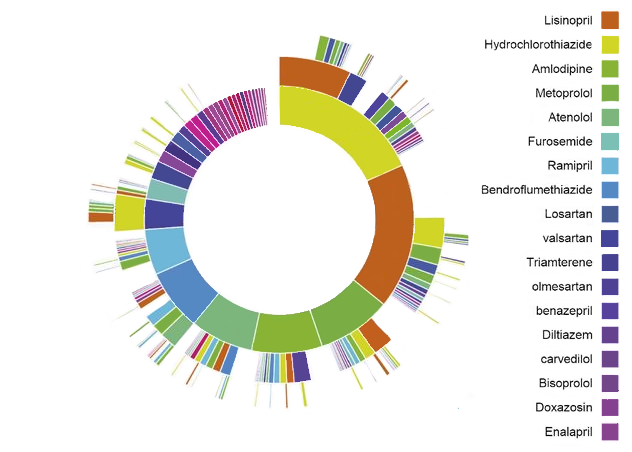
\includegraphics[width=1\linewidth]{images/Characterization/pnasTreatmentPathwaysSunburst} 

}

\caption{高血圧のためのOHDSI治療経路「サンバースト」可視化}\label{fig:treatmentPathwaysSunburstDataViz}
\end{figure}

例として、図 \ref{fig:treatmentPathwaysSunburstDataViz} は高血圧治療を開始する集団を表しています。中央にある最初のリングは、最初の治療法に基づいた人々の割合を示しています。この例では、ヒドロクロロチアジドがこの集団で最も一般的な最初の治療法です。ヒドロクロロチアジドのセクションから延びるボックスは、コホート内の人々に記録された2番目および3番目の治療法を示しています。

経路分析は、集団における治療利用に関する重要な証拠を提供します。この分析から、最初の治療法として最も一般的に利用される治療法、治療を中止する人の割合、治療を変える人、または治療を強化する人の割合を記述することができます。経路分析を使用して、\citet{Hripcsak7329} はメトホルミンが糖尿病治療のために最も一般的に処方されている薬剤であることを発見し、そこで米国内分泌学会の糖尿病治療アルゴリズムの最初の推奨事項である大規模な導入が確認されました。さらに、糖尿病患者の10\%、高血圧患者の24\%、抑うつ患者の11\%が、いずれのデータソースにも共有されていない治療経路をたどっていたことが明らかになりました。

従来のDUS(薬剤使用研究)用語では、治療経路分析は、指定された集団における一つまたは複数の薬剤の使用の普及率などの集団レベルのDUS推定値および持続性やさまざまな治療法間の切り替えの測定などの個人レベルのDUSを含みます。

\section{発生率}\label{ux767aux751fux7387}

発生率および割合は、時間の経過とともに人口における新しいアウトカムの発生を評価するための公衆衛生の統計です。図 \ref{fig:incidenceTimeline} は、単一の人に対する発生率の計算コンポーネントを示すことを目的としています: \index{incidence}

\begin{figure}

{\centering \includegraphics[width=1\linewidth]{images/Characterization/incidenceTimeline} 

}

\caption{発生率計算コンポーネントの人単位のビュー。この例では、リスク時間はコホート開始の翌日に始まり、コホート終了時に終了する。}\label{fig:incidenceTimeline}
\end{figure}

図 \ref{fig:incidenceTimeline} では、人がデータで観察される期間が観察開始と終了時間によって示されています。次に、個人がいくつかの適格基準を満たしてコホートに入る時点と出る時点があります。リスク時間ウィンドウは、アウトカムの発生を理解しようとする期間を示しています。アウトカムがリスク時間内に発生した場合、それをアウトカムの発生としてカウントします。

発生率を計算するための2つの尺度があります:

\[
発生割合 = \frac{\#\;リスク時間中に新しいアウトカムが発生したコホート内の人数}{リスク時間を持つコホート内の人数}
\]

発生割合は、リスク時間中に集団内で発生した新しいアウトカムの割合を提供します。別の言い方をすると、これは定義された時間枠内で関心集団内でアウトカムを得た割合を示します。\index{incidence!proportion}

\[
発生率 = \frac{\#\;リスク時間中に新しいアウトカムが発生したコホート内の人数}{コホート内の人々によって提供されたリスク時間}
\]

発生率は、集団の累積的なリスク時間内で新しいアウトカムの数を測定する尺度です。リスク時間中にある人がアウトカムを経験した場合、その人のリスク時間への寄与はアウトカムの発生時点で停止します。累積的なリスク時間は\textbf{人時間}と呼ばれ、日、月または年単位で表現されます。\index{incidence!rate} \index{person-time}

治療に対して計算される場合、発生割合および発生率は、特定の治療の使用の集団レベルのDUSの古典的な尺度です。

\section{高血圧患者の特性評価}\label{ux9ad8ux8840ux5727ux60a3ux8005ux306eux7279ux6027ux8a55ux4fa1}

世界保健機関(WHO)の高血圧に関するグローバル概要 \citep{WHOHypertension} によると、高血圧の早期発見、適切な治療、および良好な管理には、健康上および経済上の大きな利益が伴います。WHOの概要は、高血圧についての概観を提供し、各国における疾病の負担の特性を評価しています。WHOは、地理的地域、社会経済的クラス、および性別に関する高血圧の記述統計を提供しています。

観察研究のデータソースは、WHOが行ったように高血圧集団を特性を評価する方法を提供します。本章の後のセクションでは、ATLASおよびRを使用してデータベースを探索し、高血圧集団を研究するためのその構成を理解する方法を探ります。その後、これらのツールを使用して、高血圧集団の自然経過および治療パターンを記述します。

\section{ATLASにおけるデータベースの特性評価}\label{atlasux306bux304aux3051ux308bux30c7ux30fcux30bfux30d9ux30fcux30b9ux306eux7279ux6027ux8a55ux4fa1}

ここでは、\href{https://github.com/OHDSI/Achilles}{ACHILLES} を使用して作成されたデータベース特性評価統計を調査するために、ATLASのデータソースモジュールを使用する方法を示します。まず、ATLASの左バーで \includegraphics{images/Characterization/atlasDataSourcesMenuItem.png} をクリックして開始します。ATLASに表示される最初のドロップダウンリストで、調査するデータベースを選択します。次に、データベースの下のドロップダウンを使用してレポートを探索し始めます。これを行うには、レポートドロップダウンリストから「Condition Occurrence」を選択し、データベースに存在するすべての症状のツリーマップビジュアライゼーションを表示します:

\begin{figure}

{\centering \includegraphics[width=1\linewidth]{images/Characterization/atlasDataSourcesConditionTreemap} 

}

\caption{Atlas Data Sources: Condition Occurrence Treemap}\label{fig:atlasDataSourcesConditionTreemap}
\end{figure}

特定の関心のある症状を検索するには、テーブルタブをクリックして、データベース内のすべてのコンディションのリストを表示し、個人の数、発生率、および個人ごとの記録数を確認します。上部のフィルターボックスを使用して、コンセプト名に「hypertension」を含む項目に基づいてリストをフィルタリングできます:

\begin{figure}

{\centering \includegraphics[width=1\linewidth]{images/Characterization/atlasDataSourcesConditionFiltered} 

}

\caption{ATLASデータソース: コンセプト名に「高血圧」が含まれる疾患。}\label{fig:atlasDataSourcesConditionFiltered}
\end{figure}

特定の症状の詳細なドリルダウンレポートを表示するには、行をクリックします。この場合、「essential hypertension」を選択して、選択された症状の時系列および性別別の傾向、月別の発生率、コンディションとの共記録タイプ、および診断の初回発生時の年齢の内訳を確認します:

\begin{figure}

{\centering \includegraphics[width=1\linewidth]{images/Characterization/atlasDataSourcesDrillDownReport} 

}

\caption{ATLASデータソース: 本態性高血圧ドリルダウンレポート}\label{fig:atlasDataSourcesDrillDownReport}
\end{figure}

高血圧コンセプトの存在および時間の経過に伴う傾向についてデータベースの特性を確認した後、高血圧患者の治療に使用される薬剤を調査することもできます。これを行うには、同じ手順に従い、RxNormの成分に要約された薬剤の特性を確認するために「Drug Era」レポートを使用します。興味のある項目をレビューするためにデータベース特性を探索した後、高血圧者を特性化するためのコホートの構築を進める準備が整います。

\section{ATLASにおけるコホート特性分析}\label{atlasux306bux304aux3051ux308bux30b3ux30dbux30fcux30c8ux7279ux6027ux5206ux6790}

ここでは、ATLASを使用して複数のコホートの大規模な特性評価を行う方法を示します。左側のバーにある\includegraphics{images/Characterization/atlasCharacterizationMenuItem.png}をクリックし、新しい特性評価を作成します。分析に名前を付け、\includegraphics{images/PopulationLevelEstimation/save.png}ボタンを使用して保存します。

\subsection{デザイン}\label{ux30c7ux30b6ux30a4ux30f3}

特性の評価には、少なくとも1つのコホートと少なくとも1つの特性が必要です。この例では、2つのコホートを使用します。最初のコホートでは、高血圧治療を開始日とし、その前の1年間に少なくとも1つの高血圧診断を受けた人々を定義します。また、このコホートに属する人々が治療開始後少なくとも1年間観察期間を持つことを要求します(附録 \ref{HTN1yrFO})。2つ目のコホートは、最初のコホートと同様ですが、1年間の代わりに少なくとも3年間の観察期間を必要とします(附録 \ref{HTN3yrFO})。

\subsubsection*{コホート定義}\label{ux30b3ux30dbux30fcux30c8ux5b9aux7fa9}
\addcontentsline{toc}{subsubsection}{コホート定義}

\begin{figure}

{\centering \includegraphics[width=1\linewidth]{images/Characterization/atlasCharacterizationCohortSelection} 

}

\caption{特性設計タブ - コホート定義の選択}\label{fig:atlasCharacterizationCohortSelection}
\end{figure}

コホートは既にATLASで作成されていると仮定しています(Chapter \ref{Cohorts}を参照)。\includegraphics{images/Characterization/atlasImportButton.png}をクリックし、図 \ref{fig:atlasCharacterizationCohortSelection}に示すようにコホートを選択します。次に、これらのコホートを特性の評価するために使用する特性を定義します。

\subsubsection*{特性選択}\label{ux7279ux6027ux9078ux629e}
\addcontentsline{toc}{subsubsection}{特性選択}

ATLASにはOMOP CDMにモデル化された臨床領域全体で特性の評価を行うための約100のプリセット特性評価が付属しており、各ターゲットコホートに対して臨床観察の集約および要約機能を提供します。これらの計算は、コホートのベースラインおよびポストインデックス特性を説明するための潜在的に数千の特性を提供します。ATLASは、各コホートの特性の評価を行うために、OHDSIのFeatureExtraction Rパッケージを利用しています。次のセクションでは、FeatureExtractionとRの使用について詳しく説明します。\index{feature analyses}

\includegraphics{images/Characterization/atlasImportButton.png}をクリックして、特性を選択します。以下は、これらのコホートを特性評価するために使用する特性のリストです:

\begin{figure}

{\centering \includegraphics[width=1\linewidth]{images/Characterization/atlasCharacterizationFeatureSelection} 

}

\caption{特性設計タブ - 特性選択}\label{fig:atlasCharacterizationFeatureSelection}
\end{figure}

上図は、説明と共に選択された特性のリストを示しています。名前が「Demographics」で始まる特性は、コホート開始日における各人の人口統計情報を計算します。ドメイン名(例:Visit, Procedure, Condition, Drugなど)で始まる特性は、そのドメインにおけるすべての記録された観察を特性評価します。各ドメイン特性には4つの選択肢があります:

\begin{itemize}
\tightlist
\item
  \textbf{Any time prior}: コホート開始前のすべての利用可能な時間を使用します。
\item
  \textbf{Long term}: コホート開始日までの365日。
\item
  \textbf{Medium term}: コホート開始日までの180日。
\item
  \textbf{Short term}: コホート開始日までの30日。
\end{itemize}

\subsubsection*{サブグループ分析}\label{ux30b5ux30d6ux30b0ux30ebux30fcux30d7ux5206ux6790}
\addcontentsline{toc}{subsubsection}{サブグループ分析}

性別に基づいて異なる特性を作成したい場合、「サブグループ分析」セクションを使用して、新しい興味のあるサブグループを定義し特性評価に使用できます。

サブグループを作成するには、をクリックし、サブグループメンバーシップのための基準を追加します。このステップは、コホート登録を識別するために使用される基準と似ています。この例では、コホート内の女性を識別するための基準を定義します:

\begin{figure}

{\centering \includegraphics[width=1\linewidth]{images/Characterization/atlasCharacterizationSubgroup} 

}

\caption{特性評価の設計 - 女性サブグループ分析}\label{fig:atlasCharacterizationSubgroup}
\end{figure}

\begin{rmdimportant}
ATLASのサブグループ分析は階層とは異なります。階層は相互に排他的ですが、サブグループは選択された基準に基づいて同じ人を含む場合があります。
\end{rmdimportant}

\subsection{実行}\label{ux5b9fux884c}

特性評価のデザインが完了したら、環境内の1つ以上のデータベースに対してこのデザインを実行できます。実行タブに移動し、Generateボタンをクリックしてデータベースで分析を開始します:

\begin{figure}

{\centering \includegraphics[width=1\linewidth]{images/Characterization/atlasCharacterizationExecutions} 

}

\caption{特性評価設計の実行 - CDMソース選択}\label{fig:atlasCharacterizationExecutions}
\end{figure}

分析が完了したら、「All Executions」ボタンをクリックしてレポートを表示し、実行リストから「View Reports」を選択します。あるいは、「View latest result」をクリックして、最後に実行されたアウトカムを表示することもできます。

\subsection{結果}\label{ux7d50ux679c}

\begin{figure}

{\centering \includegraphics[width=1\linewidth]{images/Characterization/atlasCharacterizationResultsSummary} 

}

\caption{特性アウトカム - 過去1年間の疾患発生}\label{fig:atlasCharacterizationResultsSummary}
\end{figure}

結果は、選択された各コホートの異なる特性の表形式のビューを提供します。図 \ref{fig:atlasCharacterizationResultsSummary}では、コホート開始日の前の365日間に存在するすべての条件の概要が提供されています。各共変量には、コホートごとおよび定義した女性サブグループごとのカウントと割合が表示されています。

検索ボックスを使用してアウトカムをフィルタリングし、「心房細動」が履歴にある人々の割合を確認することで、集団でどのような心血管関連診断が観察されるかを理解しようとしました。「Explore」リンクをクリックして新しいウィンドウを開き、単一コホートのコンセプトに関する詳細を表示します(図 @ref(fig:atlasCharacterizationResultsExplore)に示すように)。

\begin{figure}

{\centering \includegraphics[width=1\linewidth]{images/Characterization/atlasCharacterizationResultsExplore} 

}

\caption{特性アウトカム - 単一コンセプトの探索}\label{fig:atlasCharacterizationResultsExplore}
\end{figure}

コホートのすべての条件コンセプトを特性評価したので、「explore」オプションを使用して、選択されたコンセプト(この場合は心房細動)のすべての先祖および子孫コンセプトのビューを有効にします。この探索により、高血圧のある人々に現れる可能性のある他の心疾患を探索するためにコンセプトの階層をナビゲートすることができます。要約ビューと同様に、カウントと割合が表示されます。

この特性アウトカムを使用して、アンチ高血圧治療に禁忌のある条件(例:血管浮腫)を見つけることもできます。これを行うには、上記と同じ手順を実行しますが、今回は「edema」を検索します(図 @ref(fig:atlasCharacterizationResultsContra)を参照)。

\begin{figure}

{\centering \includegraphics[width=1\linewidth]{images/Characterization/atlasCharacterizationResultsContra} 

}

\caption{特性評価の結果 - 禁忌条件の探索}\label{fig:atlasCharacterizationResultsContra}
\end{figure}

再度、「explore」機能を使用して、高血圧集団における浮腫の特性を見て血管浮腫の有病率を見つけます:

\begin{figure}

{\centering \includegraphics[width=1\linewidth]{images/Characterization/atlasCharacterizationResultsContraExplore} 

}

\caption{特性アウトカム - 禁忌条件の詳細を探索}\label{fig:atlasCharacterizationResultsContraExplore}
\end{figure}

ここでは、アンチ高血圧薬を開始する前の1年に血管浮腫の記録がある集団の一部が見つかりました。

\begin{figure}

{\centering \includegraphics[width=1\linewidth]{images/Characterization/atlasCharacterizationResultsContinuous} 

}

\caption{各コホートとサブグループの年齢特性アウトカム}\label{fig:atlasCharacterizationResultsContinuous}
\end{figure}

ドメイン共変量は、コホート開始前の時間枠にコードの記録が存在したかどうかを示す二元指標を使用して計算されますが、一部の変数はコホート開始時の年齢のように連続変数として提供されます。上の例では、カウント、平均年齢、中央値、標準偏差といった形で表現された2つのコホートの年齢を示しています。

\subsection{カスタム特性の定義}\label{ux30abux30b9ux30bfux30e0ux7279ux6027ux306eux5b9aux7fa9}

プリセット特性に加えて、ATLASはユーザー定義のカスタム特性をサポートしています。これを行うには、左側のメニューの\textbf{Characterization}をクリックし、\textbf{Feature Analysis}タブをクリックして、\textbf{New Feature Analysis}ボタンをクリックします。カスタム特性に名前を付け、\includegraphics{images/PopulationLevelEstimation/save.png}ボタンを使用して保存します。\index{ATLAS!characterization features}

この例では、ACE阻害剤の薬歴がコホート開始後にあるコホート内の人数を特定するカスタム特性を定義します:

\begin{figure}

{\centering \includegraphics[width=1\linewidth]{images/Characterization/atlasCharacterizationCustomFeature} 

}

\caption{ATLASでのカスタム特性定義}\label{fig:atlasCharacterizationCustomFeature}
\end{figure}

上で定義した基準は、コホート開始日に適用されることを前提としています。基準を定義して保存したら、前のセクションで作成した特性設計にこの基準を適用できます。特性評価設計を開き、Feature Analysisセクションに移動します。\includegraphics{images/Characterization/atlasImportButton.png}ボタンをクリックし、メニューから新しいカスタムフィーチャーを選択します。これで、特性評価設計のフィーチャーリストに表示されます。前述のように、このデザインをデータベースに対して実行して、このカスタムフィーチャーの特性分析を生成することができます:

\begin{figure}

{\centering \includegraphics[width=1\linewidth]{images/Characterization/atlasCharacterizationCustomFeatureResults} 

}

\caption{カスタムフィーチャーの結果表示}\label{fig:atlasCharacterizationCustomFeatureResults}
\end{figure}

\section{Rでのコホートの特性評価}\label{rux3067ux306eux30b3ux30dbux30fcux30c8ux306eux7279ux6027ux8a55ux4fa1}

私たちはRを使用してコホートを特徴づけることもできます。このセクションでは、OHDSI RパッケージであるFeatureExtractionを使用して、高血圧コホートのベースライン機能(共変量)を生成する方法について説明します。FeatureExtractionは、3つの方法で共変量を構築する機能を提供します。 \index{FeatureExtraction}

\begin{itemize}
\tightlist
\item
  デフォルトの共変量セットを選択する
\item
  事前に指定された分析セットから選択する
\item
  カスタム分析セットを作成する
\end{itemize}

FeatureExtractionは、個人ベースの特徴と集計された特徴の2つの異なる方法で共変量を作成します。個人ベースの特徴は機械学習アプリケーションで有用です。この章では、興味のあるコホートを説明するためのベースライン共変量を生成するために有用な集計された特徴の使用に焦点を当てます。さらに、事前に指定された分析とカスタム分析という2つの方法で共変量を構築する方法に焦点を当て、デフォルトのセットを使用する方法は読者への課題とします。

\subsection{コホートの生成}\label{ux30b3ux30dbux30fcux30c8ux306eux751fux6210}

最初に、特性を評価するためにコホートを生成する必要があります。コホートの生成は、Chapter \ref{Cohorts}で説明されています。この例では、高血圧に対して一次治療を開始し、1年間のフォローアップを行う人々を使用します(Appendix \ref{HTN1yrFO})。他のコホートの特性評価はAppendix \ref{CohortDefinitions}として残します。コホートが\texttt{scratch.my\_cohorts}というテーブルにコホート定義IDが1で生成されていることを仮定します。

\subsection{データ抽出}\label{ux30c7ux30fcux30bfux62bdux51fa}

まず、Rにサーバーへの接続方法を指示する必要があります。FeatureExtractionはDatabaseConnectorパッケージを使用し、\texttt{createConnectionDetails}という関数を提供します。さまざまなデータベース管理システム(DBMS)に必要な特定の設定については、\texttt{?createConnectionDetails}を参照してください。例えば、次のコードでPostgreSQLデータベースに接続できます:

\begin{Shaded}
\begin{Highlighting}[]
\FunctionTok{library}\NormalTok{(FeatureExtraction)}
\NormalTok{connDetails }\OtherTok{\textless{}{-}} \FunctionTok{createConnectionDetails}\NormalTok{(}\AttributeTok{dbms =} \StringTok{"postgresql"}\NormalTok{,}
                                       \AttributeTok{server =} \StringTok{"localhost/ohdsi"}\NormalTok{,}
                                       \AttributeTok{user =} \StringTok{"joe"}\NormalTok{,}
                                       \AttributeTok{password =} \StringTok{"supersecret"}\NormalTok{)}

\NormalTok{cdmDbSchema }\OtherTok{\textless{}{-}} \StringTok{"my\_cdm\_data"}
\NormalTok{cohortsDbSchema }\OtherTok{\textless{}{-}} \StringTok{"scratch"}
\NormalTok{cohortsDbTable }\OtherTok{\textless{}{-}} \StringTok{"my\_cohorts"}
\NormalTok{cdmVersion }\OtherTok{\textless{}{-}} \StringTok{"5"}
\end{Highlighting}
\end{Shaded}

最後の4行は、\texttt{cdmDbSchema}、\texttt{cohortsDbSchema}、\texttt{cohortsDbTable}変数、およびCDMバージョンを定義します。これらを使用して、CDM形式のデータがどこにあるか、興味のあるコホートがどこに作成されたか、および使用されるCDMバージョンをRに通知します。Microsoft SQL Serverの場合、データベーススキーマはデータベースとスキーマの両方を指定する必要があることに注意してください。したがって、例えば\texttt{cdmDbSchema\ \textless{}-\ "my\_cdm\_data.dbo"}となります。

\subsection{事前に指定された分析の使用}\label{ux4e8bux524dux306bux6307ux5b9aux3055ux308cux305fux5206ux6790ux306eux4f7fux7528}

\texttt{createCovariateSettings}関数は、ユーザーが多くの定義済みの共変量から選択できるようにします。利用可能なオプションの概要については、\texttt{?createCovariateSettings}を参照してください。例を示します:

\begin{Shaded}
\begin{Highlighting}[]
\NormalTok{settings }\OtherTok{\textless{}{-}} \FunctionTok{createCovariateSettings}\NormalTok{(}
  \AttributeTok{useDemographicsGender =} \ConstantTok{TRUE}\NormalTok{,}
  \AttributeTok{useDemographicsAgeGroup =} \ConstantTok{TRUE}\NormalTok{,}
  \AttributeTok{useConditionOccurrenceAnyTimePrior =} \ConstantTok{TRUE}\NormalTok{)}
\end{Highlighting}
\end{Shaded}

これにより、性別、年齢(5年ごとの年齢グループ)、およびコホート開始日までの期間に観察された各コンセプトについての二進共変量が作成されます。

多くの事前に指定された分析は、短期、中期、長期の時間枠を参照しています。デフォルトでは、これらの枠は次のように定義されています:

\begin{itemize}
\tightlist
\item
  \textbf{長期}: コホート開始日を含む365日前まで
\item
  \textbf{中期}: コホート開始日を含む180日前まで
\item
  \textbf{短期}: コホート開始日を含む30日前まで
\end{itemize}

ただし、ユーザーはこれらの値を変更できます。例を示します:

\begin{Shaded}
\begin{Highlighting}[]
\NormalTok{settings }\OtherTok{\textless{}{-}} \FunctionTok{createCovariateSettings}\NormalTok{(}\AttributeTok{useConditionEraLongTerm =} \ConstantTok{TRUE}\NormalTok{,}
                                    \AttributeTok{useConditionEraShortTerm =} \ConstantTok{TRUE}\NormalTok{,}
                                    \AttributeTok{useDrugEraLongTerm =} \ConstantTok{TRUE}\NormalTok{,}
                                    \AttributeTok{useDrugEraShortTerm =} \ConstantTok{TRUE}\NormalTok{,}
                                    \AttributeTok{longTermStartDays =} \SpecialCharTok{{-}}\DecValTok{180}\NormalTok{,}
                                    \AttributeTok{shortTermStartDays =} \SpecialCharTok{{-}}\DecValTok{14}\NormalTok{,}
                                    \AttributeTok{endDays =} \SpecialCharTok{{-}}\DecValTok{1}\NormalTok{)}
\end{Highlighting}
\end{Shaded}

これにより、長期の枠はコホート開始日を含まない180日前まで、短期の枠はコホート開始日を含まない14日前までに再定義されます。

また、どのコンセプトIDを使用するかしないかを指定することもできます:

\begin{Shaded}
\begin{Highlighting}[]
\NormalTok{settings }\OtherTok{\textless{}{-}} \FunctionTok{createCovariateSettings}\NormalTok{(}\AttributeTok{useConditionEraLongTerm =} \ConstantTok{TRUE}\NormalTok{,}
                                    \AttributeTok{useConditionEraShortTerm =} \ConstantTok{TRUE}\NormalTok{,}
                                    \AttributeTok{useDrugEraLongTerm =} \ConstantTok{TRUE}\NormalTok{,}
                                    \AttributeTok{useDrugEraShortTerm =} \ConstantTok{TRUE}\NormalTok{,}
                                    \AttributeTok{longTermStartDays =} \SpecialCharTok{{-}}\DecValTok{180}\NormalTok{,}
                                    \AttributeTok{shortTermStartDays =} \SpecialCharTok{{-}}\DecValTok{14}\NormalTok{,}
                                    \AttributeTok{endDays =} \SpecialCharTok{{-}}\DecValTok{1}\NormalTok{,}
                                    \AttributeTok{excludedCovariateConceptIds =} \DecValTok{1124300}\NormalTok{,}
                                    \AttributeTok{addDescendantsToExclude =} \ConstantTok{TRUE}\NormalTok{,}
                                    \AttributeTok{aggregated =} \ConstantTok{TRUE}\NormalTok{)}
\end{Highlighting}
\end{Shaded}

\begin{rmdimportant}
上記すべての例について、「aggregated = TRUE」の使用は、FeatureExtractionに要約統計を提供することを指示します。このフラグを除外すると、コホート内の各個人の共変量が計算されます。
\end{rmdimportant}

\subsection{集計された共変量の作成}\label{ux96c6ux8a08ux3055ux308cux305fux5171ux5909ux91cfux306eux4f5cux6210}

次のコードブロックは、コホートの集計統計を生成します:

\begin{Shaded}
\begin{Highlighting}[]
\NormalTok{covariateSettings }\OtherTok{\textless{}{-}} \FunctionTok{createDefaultCovariateSettings}\NormalTok{()}

\NormalTok{covariateData2 }\OtherTok{\textless{}{-}} \FunctionTok{getDbCovariateData}\NormalTok{(}
  \AttributeTok{connectionDetails =}\NormalTok{ connectionDetails,}
  \AttributeTok{cdmDatabaseSchema =}\NormalTok{ cdmDatabaseSchema,}
  \AttributeTok{cohortDatabaseSchema =}\NormalTok{ resultsDatabaseSchema,}
  \AttributeTok{cohortTable =} \StringTok{"cohorts\_of\_interest"}\NormalTok{,}
  \AttributeTok{cohortId =} \DecValTok{1}\NormalTok{,}
  \AttributeTok{covariateSettings =}\NormalTok{ covariateSettings,}
  \AttributeTok{aggregated =} \ConstantTok{TRUE}\NormalTok{)}

\FunctionTok{summary}\NormalTok{(covariateData2)}
\end{Highlighting}
\end{Shaded}

出力は次のようになります:

\begin{verbatim}

## CovariateData Object Summary
##

## Number of Covariates: 41330

## Number of Non-Zero Covariate Values: 41330
\end{verbatim}

\subsection{出力形式}\label{ux51faux529bux5f62ux5f0f}

集計された\texttt{covariateData}オブジェクトの主なコンポーネントは、二値および連続的な共変量に対してそれぞれ\texttt{covariates}および\texttt{covariatesContinuous}です:

\begin{Shaded}
\begin{Highlighting}[]
\NormalTok{covariateData2}\SpecialCharTok{$}\NormalTok{covariates}
\NormalTok{covariateData2}\SpecialCharTok{$}\NormalTok{covariatesContinuous}
\end{Highlighting}
\end{Shaded}

\subsection{カスタム共変量}\label{ux30abux30b9ux30bfux30e0ux5171ux5909ux91cf}

FeatureExtractionは、カスタム共変量を定義および利用する能力も提供します。これについての詳細は高度なトピックであり、ユーザードキュメントに記載されています:\url{http://ohdsi.github.io/FeatureExtraction/}

\section{ATLASにおけるコホートパスウェイ分析}\label{atlasux306bux304aux3051ux308bux30b3ux30dbux30fcux30c8ux30d1ux30b9ux30a6ux30a7ux30a4ux5206ux6790}

パスウェイ分析の目標は、1つ以上の興味のあるコホート内で治療がどのように順序づけられているかを理解することです。\href{mailto:適用される方法は@Hripcsak7329}{\nolinkurl{適用される方法は@Hripcsak7329}} によって報告された設計に基づいています。これらの方法は一般化され、ATLASのCohort Pathwaysという機能に組み込まれました。

コホートパスウェイの目的は、1つ以上のターゲットコホートのコホート開始日以降のイベントを要約する分析機能を提供することです。そのために、対象となる人口の臨床イベントを特定するためのイベントコホートと呼ばれるコホートセットを作成します。これがターゲットコホート内の人物に対してどのように見えるかを例として示します。

\begin{figure}

{\centering \includegraphics[width=1\linewidth]{images/Characterization/pathwaysPersonEventView} 

}

\caption{単一の人物におけるパスウェイ分析の文脈}\label{fig:pathwaysPersonEventView}
\end{figure}

図 \ref{fig:pathwaysPersonEventView} では、その人物が開始日と終了日が定義されたターゲットコホートの一部であることを示しています。その後、番号付きの線分は、その人物が特定の期間、イベントコホートとしても特定される場所を示しています。イベントコホートは、CDMに表された任意の臨床イベントを記述することができるため、単一のドメインまたはコンセプトに対してパスウェイを作成する必要はありません。

まず、ATLASの左側のバーで \includegraphics{images/Characterization/atlasPathwaysMenuItem.png} をクリックして、新しいコホートパスウェイスタディを作成します。説明的な名前を提供し、保存ボタンを押します。

\subsection{設計}\label{ux8a2dux8a08}

まず、1年および3年のフォローアップ付きの高血圧の初回治療を開始するコホートを引き続き使用します(Appendix \ref{HTN1yrFO}, \ref{HTN3yrFO})。ボタンを使用して2つのコホートをインポートします。

\begin{figure}

{\centering \includegraphics[width=1\linewidth]{images/Characterization/atlasPathwaysTargetCohorts} 

}

\caption{ターゲットコホートを選択したパスウェイ分析}\label{fig:atlasPathwaysTargetCohorts}
\end{figure}

次に、興味のある各一線級降圧薬のイベントコホートを作成して、イベントコホートを定義します。まず、ACE阻害剤の使用者のコホートを作成し、コホートの終了日を連続投与の終了日と定義します。同様に他の8つの降圧薬のコホートも作成し、これらの定義はAppendix \ref{ACEiUse}-\ref{A1BUse}に記載してあります。完了したら、\includegraphics{images/Characterization/atlasImportButton.png} ボタンを使用して、これらをパスウェイデザインのイベントコホートセクションにインポートします。

\begin{figure}

{\centering \includegraphics[width=1\linewidth]{images/Characterization/atlasPathwaysEventCohorts} 

}

\caption{初回一線級降圧治療を開始するためのイベントコホート}\label{fig:atlasPathwaysEventCohorts}
\end{figure}

完了すると、設計は上記のようになるはずです。次に、いくつかの追加の分析設定を決定する必要があります:

\begin{itemize}
\tightlist
\item
  \textbf{組み合わせウィンドウ}: この設定では、イベント間の重複がイベントの組み合わせと見なされる日数の期間を定義できます。たとえば、2つのイベントコホート(イベントコホート1およびイベントコホート2)で表される2つの薬剤が組み合わせウィンドウ内で重複する場合、パスウェイアルゴリズムはそれらを「イベントコホート1 + イベントコホート2」として組み合わせます。
\item
  \textbf{最小セル数}: この数未満の人数のイベントコホートは、プライバシーを保護するために出力から除外されます。
\item
  \textbf{最大経路長}: 分析の対象となる一連のイベントの最大数を指します。
\end{itemize}

\subsection{実行}\label{ux5b9fux884c-1}

パスウェイ分析の設計が完了すると、環境内の1つ以上のデータベースに対してこの設計を実行できます。これは、ATLASでのコホートの特性評価で説明したのと同じ方法で機能します。完了したら、分析アウトカムを確認できます。

\subsection{結果の表示}\label{ux7d50ux679cux306eux8868ux793a}

\begin{figure}

{\centering \includegraphics[width=1\linewidth]{images/Characterization/atlasPathwaysResults} 

}

\caption{パスウェイアウトカムの凡例とサンバーストビジュアライゼーション}\label{fig:atlasPathwaysResults}
\end{figure}

パスウェイ分析のアウトカムは3つのセクションに分かれています:凡例セクションでは、ターゲットコホートの総人数と、パスウェイ分析で1つ以上のイベントがあった人数が表示されます。その下には、サンバーストプロットの中央セクションに表示される各コホートのカラーコードが表示されます。

サンバーストプロットは、時間の経過に伴うさまざまなイベントパスウェイを表すビジュアライゼーションです。プロットの中心はコホートのエントリを表しており、最初のカラーディングは各イベントコホートにいる人々の割合を示しています。例では、円の中心は一線級治療を開始した高血圧者を示しています。その後、サンバーストプロットの最初のリングは、イベントコホート(例えば、ACE阻害剤、アンジオテンシン受容体遮断剤など)で定義された一線級治療を開始した人々の割合を示します。次のリングセットは、特定のイベントシーケンスにおいて2番目のイベントコホートを示します。データ内で2番目のイベントコホートが観察されない人々の割合は、リングの灰色の部分で表されます。

\begin{figure}

{\centering \includegraphics[width=1\linewidth]{images/Characterization/atlasPathwaysResultsPathDetails} 

}

\caption{経路の詳細を表示するパスウェイアウトカム}\label{fig:atlasPathwaysResultsPathDetails}
\end{figure}

サンバーストプロットのセクションをクリックすると、右側に経路の詳細が表示されます。ここでは、ターゲットコホート内の最も多くの人々がACE阻害剤で一線級治療を開始し、そのグループから少数の人々がチアジド系利尿薬を開始していることがわかります。

\section{ATLAS における発生率分析}\label{atlas-ux306bux304aux3051ux308bux767aux751fux7387ux5206ux6790}

発生率計算では、ターゲットコホート内の人々のうち、リスク期間中にアウトカムコホートを経験した人を記述します。ここでは、ACE阻害薬 (ACEi) およびチアジド系およびチアジド様利尿薬 (THZ) の新規使用者における血管浮腫 (Angioedema) および急性心筋梗塞 (AMI) のアウトカムの特性を評価するための発生率分析を設計します。これらのアウトカムを、薬剤に曝露されている期間 (TAR) 中に評価します。さらに、ターゲットコホート (ACEi および THZ) への曝露中に新規のアンジオテンシン受容体拮抗薬 (ARB) 使用の発生率を測定するために、ARB の使用アウトカムを追加します。このアウトカム定義は、ターゲット集団の中で ARB の利用方法を理解するためのものです。

始めるには、ATLAS の左バーにある \includegraphics{images/Characterization/atlasIncidenceMenuItem.png} をクリックして新しい発生率分析を作成します。説明的な名前を提供し、保存ボタン \includegraphics{images/PopulationLevelEstimation/save.png} を押します。

\subsection{設計}\label{ux8a2dux8a08-1}

本例で使用されるコホートは、既に ATLAS に作成されていると仮定します (Chapter \ref{Cohorts} で説明)。付録には、ターゲットコホート (Appendix \ref{AceInhibitorsMono}, \ref{ThiazidesMono}) およびアウトカムコホート (Appendix \ref{Angioedema}, \ref{Ami}, \ref{ARBUse}) の完全な定義が提供されています。

\begin{figure}

{\centering \includegraphics[width=1\linewidth]{images/Characterization/atlasIncidenceCohortSelection} 

}

\caption{ターゲットおよびアウトカム定義の発生率。}\label{fig:atlasIncidenceCohortSelection}
\end{figure}

定義タブで、 \emph{New users of ACE inhibitors} コホートと \emph{New users of Thiazide or Thiazide-like diuretics} コホートを選択します。ダイアログを閉じて、これらのコホートが設計に追加されたことを確認します。次に、アウトカムコホートを追加するためにクリックし、ダイアログボックスから \emph{acute myocardial infarction events} 、 \emph{angioedema events} 、および \emph{Angiotensin receptor blocker (ARB) use} のアウトカムコホートを選択します。再びウィンドウを閉じて、これらのコホートが設計のアウトカムコホートセクションに追加されたことを確認します。

\begin{figure}

{\centering \includegraphics[width=1\linewidth]{images/Characterization/atlasIncidenceTimeAtRisk} 

}

\caption{ターゲットおよびアウトカム定義の発生率。}\label{fig:atlasIncidenceTimeAtRisk}
\end{figure}

次に、分析のリスク時間枠を定義します。上に示すように、リスク時間枠はコホートの開始日および終了日と相対しています。ここでは、ターゲットコホートの開始日の翌日をリスク時間枠の開始として定義します。次に、リスク時間枠をコホートの終了日に終了するよう定義します。この場合、ACEi および THZ コホートの定義には、薬剤曝露が終了する時点をコホート終了日としています。

ATLAS では、分析仕様の一部としてターゲットコホートを層化する方法も提供されています:

\begin{figure}

{\centering \includegraphics[width=1\linewidth]{images/Characterization/atlasIncidenceStratifyFemale} 

}

\caption{女性のための発生率層定義。}\label{fig:atlasIncidenceStratifyFemale}
\end{figure}

これを行うには、{[}新しい層化基準{]} ボタンをクリックし、Chapter 11 で説明されている手順に従います。設計が完了したので、一つ以上のデータベースに対して設計を実行に移ることができます。

\subsection{実行}\label{ux5b9fux884c-2}

{[}生成{]} タブをクリックし、 \includegraphics{images/Characterization/atlasIncidenceGenerate.png} ボタンをクリックして、分析を実行するデータベースの一覧を表示します:

\begin{figure}

{\centering \includegraphics[width=1\linewidth]{images/Characterization/atlasIncidenceSourceSelection} 

}

\caption{発生率分析実行。}\label{fig:atlasIncidenceSourceSelection}
\end{figure}

一つ以上のデータベースを選択し、{[}生成{]} ボタンをクリックして、設計で指定されたターゲットとアウトカムのすべての組み合わせを分析するために分析を開始します。

\subsection{結果の表示}\label{ux7d50ux679cux306eux8868ux793a-1}

生成タブでは、画面の上部でターゲットおよびアウトカムを選択してアウトカムを表示することができます。このすぐ下には、分析で使用された各データベースの発生率のサマリーが表示されます。

それらのドロップダウンリストから ACEi 使用者のターゲットコホートと急性心筋梗塞 (AMI) を選択します。\includegraphics{images/Characterization/atlasIncidenceReportButton.png} ボタンをクリックして発生率分析のアウトカムを表示します:

\begin{figure}

{\centering \includegraphics[width=1\linewidth]{images/Characterization/atlasIncidenceResults} 

}

\caption{発生率分析の出力 - AMI のアウトカムを持つ新規 ACEi 使用者。}\label{fig:atlasIncidenceResults}
\end{figure}

データベースのサマリーは、TAR 期間中に観察されたコホート内の総人数と総症例数を示します。割合は 1000人当たりの症例数を示しています。ターゲットコホートのリスク時間は年単位で計算されます。発生率は 1000人年当たりの症例数として表されます。

設計で定義した層の発生率メトリクスも見ることができます。上記のメトリクスは各層についても計算されます。さらに、ツリーマップビジュアライゼーションは、それぞれの層が表す割合をボックスエリアとして視覚的に表示します。色は、底部に示されるスケールに沿って発生率を示しています。

ACEi 集団の中で ARB 新規使用の発生率を確認するための同じ情報を収集することができます。画面上部のドロップダウンでアウトカムを ARB 使用に変更し、 \includegraphics{images/Characterization/atlasIncidenceReportButton.png} ボタンをクリックして詳細を確認します。

\begin{figure}

{\centering \includegraphics[width=1\linewidth]{images/Characterization/atlasIncidenceResultsARB} 

}

\caption{発生率 - ACEi 曝露中に ARB 処理を受けている新規 ACEi 使用者。}\label{fig:atlasIncidenceResultsARB}
\end{figure}

示されているように、計算されたメトリクスは同じですが、解釈は異なります。入力 (ARB 使用) が薬剤利用推定を参照しているため、健康アウトカムではありません。

\section{まとめ}\label{ux307eux3068ux3081-8}

\begin{rmdsummary}
\begin{itemize}
\item
  OHDSI は、データベース全体または関心のあるコホートの特性を評価するためのツールを提供します。
\item
  コホートの特徴付けは、インデックス日(基準)前およびインデックス日後(ポストインデックス)の期間に関心のあるコホートを記述します。
\item
  ATLAS の特徴付けモジュールおよび OHDSI メソッドライブラリは、複数の時間枠の基準特性を計算する機能を提供します。
\item
  ATLAS の経路および発生率モジュールは、ポストインデックス期間中の記述統計を提供します。
\end{itemize}
\end{rmdsummary}

\section{演習}\label{ux6f14ux7fd2-4}

\subsubsection*{前提条件}\label{ux524dux63d0ux6761ux4ef6-6}
\addcontentsline{toc}{subsubsection}{前提条件}

これらの演習には、ATLAS インスタンスへのアクセスが必要です。\url{http://atlas-demo.ohdsi.org} のインスタンスや、アクセス可能なその他のインスタンスを使用できます。

\begin{exercise}
\protect\hypertarget{exr:exerciseCharacterization1}{}\label{exr:exerciseCharacterization1}私たちは、実際の世界でセレコキシブがどのように使用されているかを理解したいと考えています。始めに、この薬剤に関するデータベースの情報を理解したいと考えています。ATLAS のデータソースモジュールを使用して、セレコキシブに関する情報を見つけてください。
\end{exercise}

\begin{exercise}
\protect\hypertarget{exr:exerciseCharacterization2}{}\label{exr:exerciseCharacterization2}セレコキシブ使用者の疾患の自然の歴史をより理解したいと考えています。365 日のウォッシュアウト期間を使用して、セレコキシブの新規使用者の単純なコホートを作成し、このコホートの特性評価を作成し、併存疾患および薬剤曝露を示してください (Chapter \ref{Cohorts} で詳細な手順があります)。
\end{exercise}

\begin{exercise}
\protect\hypertarget{exr:exerciseCharacterization3}{}\label{exr:exerciseCharacterization3}セレコキシブ処方開始後に消化管出血 (GI 出血) がどのくらいの頻度で発生するのかに興味があります。\href{http://athena.ohdsi.org/search-terms/terms/192671}{192671} (``消化管出血'') またはその子孫のいずれかのコンセプトの発生として単純に定義される GI 出血イベントのコホートを作成します。前の演習で定義した曝露コホートを使用して、セレコキシブ開始後のこれらの GI 出血イベントの発生率を計算してください。
\end{exercise}

提案された解答は Appendix \ref{Characterizationanswers} に記載されています。

\chapter{第12章 --翻訳作業中-- 集団レベルの推定}\label{PopulationLevelEstimation}

\emph{チャプターリード: Martijn Schuemie, David Madigan, Marc Suchard \& Patrick Ryan}

\index{population-level estimation}

保険請求データや電子健康記録などの観察的な医療データは、治療の効果に関する現実世界のエビデンスを生成する機会を提供し、患者の生活を有意に改善することができます。本章では、特定の健康アウトカムに対する曝露(例えば、薬剤曝露や処置などの医療介入)の平均的な因果効果の推定を指す集団レベルの効果推定に焦点を当てます。以下では、2つの異なる推定タスクを検討します:

\begin{itemize}
\tightlist
\item
  \textbf{直接効果推定}: アウトカムのリスクに対する曝露の効果を、曝露なしと比較して推定する。 \index{direct effect estimation}
\item
  \textbf{比較効果推定}: アウトカムのリスクに対する曝露(ターゲット曝露)の効果を、別の曝露(比較曝露)と比較して推定する。 \index{comparative effect estimation}
\end{itemize}

いずれの場合でも、患者レベルの因果効果は事実のアウトカム、すなわち曝露を受けた患者に何が起こったかと、反事実のアウトカム、すなわち曝露がなかった場合(直接)や異なる曝露があった場合(比較)に何が起こったかを対比させます。各患者は事実のアウトカムのみを明らかにするため(因果推論の基本問題)、さまざまな効果推定デザインは異なるデバイスを使用して反事実のアウトカムを明らかにします。 \index{counterfactual}

集団レベルの効果推定のユースケースには、治療選択、安全性監視、および比較効果が含まれます。方法論は、特定の仮説を一度に1つずつテストすること(例:「シグナル評価」)や、複数の仮説を一度に探索すること(例:「シグナル検出」)ができます。いずれの場合も、目的は同じです:因果効果の高品質な推定を生成することです。 \index{safety surveillance} \index{comparative effectiveness|see {comparative effect estimation}}

本章ではまず、\href{https://ohdsi.github.io/MethodsLibrary/}{OHDSI Methods Library}としてRパッケージで実装されているさまざまな集団レベルの推定研究デザインについて説明します。次に、具体的な推定研究の設計を詳細に説明し、ATLASおよびRを使用して設計を実装する手順ガイドを提供します。最後に、研究から生成されるさまざまな出力、包括的な研究診断および効果サイズの推定についてレビューします。

\section{コホートメソッド設計}\label{CohortMethod}

\index{コホートメソッド}

\begin{figure}

{\centering \includegraphics[width=0.9\linewidth]{images/PopulationLevelEstimation/cohortMethod} 

}

\caption{新規ユーザーコホートデザイン。ターゲット治療を開始した被験者は比較対照治療を開始した被験者と比較されます。2つの治療グループ間の違いを調整するために、傾向スコアによる層化、マッチング、または重み付け、あるいはベースライン特性をアウトカムモデルに追加するなど、いくつかの調整戦略が使用されます。傾向スコアモデルまたはアウトカムモデルに含まれる特性は治療開始前に取得されます。}\label{fig:cohortMethod}
\end{figure}

コホートメソッドはランダム化臨床試験を模倣することを試みます \citep[ ]{hernan_2016}。 ある治療(ターゲット)を開始した被験者は別の治療(比較対照)を開始した被験者と比較され、治療開始後の特定の期間、例えば治療を継続する期間にわたって追跡されます。コホート研究において我々が答えたい質問は、表\ref{tab:cmChoices}にハイライトされた5つの選択を行うことで具体化されます。 \index{ターゲットコホート!コホートメソッド} \index{比較対照コホート} \index{アウトカムコホート!コホートメソッド}

表: \label{tab:cmChoices} 比較コホートデザインの主要な設計選択。

\begin{longtable}[]{@{}
  >{\raggedright\arraybackslash}p{(\columnwidth - 2\tabcolsep) * \real{0.2468}}
  >{\raggedright\arraybackslash}p{(\columnwidth - 2\tabcolsep) * \real{0.7532}}@{}}
\toprule\noalign{}
\begin{minipage}[b]{\linewidth}\raggedright
選択
\end{minipage} & \begin{minipage}[b]{\linewidth}\raggedright
説明
\end{minipage} \\
\midrule\noalign{}
\endhead
\bottomrule\noalign{}
\endlastfoot
ターゲットコホート & ターゲット治療を代表するコホート \\
比較対照コホート & 比較対照治療を代表するコホート \\
アウトカムコホート & 関心のあるアウトカムを代表するコホート \\
リスク期間 & どの時点で(通常はターゲットおよび比較対照コホートの開始および終了日)アウトカムのリスクを考慮するか \\
モデル & ターゲットと比較対照の間の違いを調整しながら効果を推定するために使用されるモデル \\
\end{longtable}

モデルの選択には、他の要素の中でも、アウトカムモデルの種類が含まれます。例えば、ロジスティック回帰を使用することができ、これはアウトカムが発生したかどうかを評価し、オッズ比を生成します。ロジスティック回帰はリスク期間がターゲットと比較対照で同じ長さであるか、または関係がないと仮定します。代替的に、定常発生率を仮定するポアソン回帰を選ぶこともできます。よく使用されるのは、リスク比を推定するための初回アウトカムまでの時間を考慮するコックス回帰であり、ターゲットと比較対照間で比例ハザードを仮定します。 \index{ロジスティック回帰} \index{ポアソン回帰} \index{コックス回帰} \index{コックス比例ハザードモデル|see {コックス回帰}}

\begin{rmdimportant}
新規ユーザーコホートメソッドは本質的に比較効果推定の方法であり、治療を比較対照と比較します。この方法を使用して治療対未治療を比較するのは難しいです。なぜなら、未曝露群と曝露群が比較可能な群を定義するのが難しいからです。この設計を直接的な効果推定に使用したい場合は、関心のある曝露に対する比較対照として、同じ適応症に対する治療を選択するのが望ましいです。ただし、必ずしもそのような比較対照が利用可能であるとは限りません。
\end{rmdimportant}

重要な懸念は、ターゲット治療を受ける患者が比較対照治療を受ける患者と系統的に異なる可能性があることです。例えば、ターゲットコホートが平均60歳であり、比較対照コホートが平均40歳であるとします。年齢に関連する健康アウトカム(例:脳卒中)に関してターゲットと比較対照を比較する場合、コホート間で顕著な違いが見られるかもしれません。無知な研究者は、ターゲット治療と比較対照に比べて脳卒中の間に因果関係があると結論づけるかもしれません。もっと平凡な、あるいはありふれた結論として、ターゲット患者が脳卒中を経験したことが、比較対照を受けていたらそうならなかったであろうと結論づけるかもしれません。この結論は完全に間違っている可能性があります!おそらくこれらのターゲット患者は、ただ年を取っているだけで脳卒中が発生したかもしれません。治療を受けていたとしても同様であった可能性があります。この文脈では、年齢は「交絡因子(コンファウンダー)」です。観察研究で交絡因子に対処する一つのメカニズムは傾向スコアを介することです。 \index{交絡因子}

\subsection{傾向スコア}\label{ux50beux5411ux30b9ux30b3ux30a2}

\index{傾向スコア}

ランダム化試験では、(仮想的な)コイントスが患者を各グループに割り当てます。したがって、設計によって、患者がターゲット治療を受ける確率は患者の特性(例:年齢)とは無関係です。コインは患者を知りませんし、何よりも、ターゲット曝露を受ける患者の確率を正確にはっきりと知っています。そのアウトカム、試験の患者数が増えるにつれて、両方のグループの患者はどのような患者特性においても体系的に異なることは基本的にできません。このバランスの保証は、試験が測定した特性(例:年齢)および試験が測定しなかった特性(例:患者の遺伝的要因)にも適用されます。 \index{ランダム化試験}

ある患者に対する\emph{傾向スコア(PS)}は、その患者がターゲット治療を受ける確率です \citep[ ]{rosenbaum_1983}。 バランスの取れた二群ランダム化試験では、傾向スコアはすべての患者に対して0.5です。傾向スコアで補正された観察研究では、治療開始時およびその前のデータに基づいて患者がターゲット治療を受ける確率を推定します(実際に受けた治療に関係なく)。これは単純な予測モデリングの応用です。ロジスティック回帰などのモデルを適合させ、患者がターゲット治療を受けるかどうかを予測し、各被験者の予測確率(PS)を生成するためにこのモデルを使用します。標準的なランダム化試験とは異なり、異なる患者は異なるターゲット治療を受ける確率を持ちます。PSは、PSが似たターゲット被験者と比較対照被験者をマッチングする、PSに基づいて研究集団を層化する、PSから導き出された治療重み付けの逆確率(IPTW)を使うなど、いくつかの方法で使用できます。マッチングの場合、各ターゲット被験者に対して一人の比較対照被験者だけを選択することも、一人以上の比較対照被験者を許容することもできます。これを可変比マッチングと言います \citep[ ]{rassen_2012}。 \index{傾向スコアモデル} \index{傾向スコア!マッチング} \index{傾向スコア!層化} \index{傾向スコア!重み付け} \index{治療重み付けの逆確率 (IPTW)|see {傾向スコア!重み付け}} \index{可変比マッチング}

例えば、一対一のPSマッチングを用いるとします。Janのターゲット治療を受ける事前確率が0.4であり、実際にターゲット治療を受けたとします。もし、事前確率0.4でターゲット治療を受けるはずだったが実際には比較対照を受けた患者(Junという名前)が見つかれば、JanとJunのアウトカムを比較することは、測定された交絡因子に関しては、小規模なランダム化試験のようなものです。この比較は、ランダム化によって生成されるJan-Jun因果コントラストの推定をもたらします。次に、推定手順は次のようになります:ターゲットを受けた各患者に対して、事前確率が同じで比較対照を受けた一人以上の患者を見つけ、これらのマッチング群内でターゲット患者のアウトカムを比較対照患者のアウトカムと比較します。

傾向スコアは測定された交絡因子を制御します。実際、測定された特性がない場合、採用された推定方法に基づいて誤差のない因果効果の推定値が得られます。測定された特性は「強い無視可能性」を仮定します。 ``強い無視可能性''は実際にはテストできない前提です。この問題についての詳細はChapter \ref{MethodValidity}で説明します。 \index{強い無視可能性}

\subsection{変数選択}\label{VariableSelection}

以前は、PSは手動で選択された特性に基づいて計算されていましたが、OHDSIツールはそのような実践をサポートする一方で、特定の曝露およびアウトカムに基づいて選択されていない、より多くの汎用特性を使用することを好みます \citep[ ]{tian_2018} 。これらの特性には、人口統計情報、治療開始前および当日に観察された診断、薬剤曝露、測定値、および医療処置が含まれます。通常、モデルには10,000から100,000の特有の特性が含まれ、これらを大規模な正則化回帰\citep[ ]{suchard_2013}を使用して適合させ、\href{https://ohdsi.github.io/Cyclops/}{Cyclops}パッケージで実装します。本質的には、どの特性が治療割り当ての予測に関連するかをデータに決定させ、モデルに含めます。

\begin{rmdimportant}
典型的には、治療開始日の特性は治療の原因となる診断などの多くの関連データがその日に記録されているため、共変量収集ウィンドウに含まれるべきです。この日には、ターゲットおよび比較対照の治療自体も記録されているが、これらは傾向スコアモデルに含まれるべきではありません。なぜなら、私たちはまさにこれらを予測しようとしているからです。したがって、ターゲットおよび比較対照治療は共変量セットから明示的に除外する必要があります。
\end{rmdimportant}

一部の人々は、因果構造を特定するために臨床専門知識に依存しない共変量選択のデータ駆動型アプローチは、誤っていわゆる道具変数や交絡因子を含め、分散を増加させ、潜在的にバイアスを導入するリスクがあると主張します。しかし、これらの懸念は現実的なシナリオでは大きな影響を与える可能性は低いです。さらに、医学においては真の因果構造が判明することはほとんどなく、異なる研究者が特定の研究問題に対して「正しい」共変量を特定するように求められると、それぞれの研究者は必ず異なるリストを作成し、そのプロセスを再現不能にします。最も重要なのは、傾向スコアモデルの確認、すべての共変量のバランス評価、および否定的対照の含有などの診断によって、交絡因子や道具変数に関連するほとんどの問題を特定できることです。 \index{道具変数} \index{交絡因子}

\subsection{カリパー}\label{ux30abux30eaux30d1ux30fc}

\index{カリパー}

傾向スコアは0から1の連続体上にあるため、厳密なマッチングはほとんど不可能です。代わりに、マッチングプロセスはターゲット患者の傾向スコアと一致する患者を「カリパー」として知られる許容範囲内で見つけます。\citet{austin_2011} に従い、ロジットスケールで標準偏差の0.2を使用します。

\subsection{オーバーラップ:偏好スコア}\label{ux30aaux30fcux30d0ux30fcux30e9ux30c3ux30d7ux504fux597dux30b9ux30b3ux30a2}

\index{偏好スコア}

傾向スコア方法は一致する患者が存在することを必要とします。このため、主要な診断は二つのグループの傾向スコアの分布を示します。解釈を容易にするために、OHDSIツールは「偏好スコア」と呼ばれる傾向スコアの変換をプロットします。偏好スコアは二つの治療の「市場占有率」を調整します。例えば、10\%の患者がターゲット治療を受ける場合(比較対照治療を受ける患者が90\%の場合)、偏好スコアが0.5の患者はターゲット治療を受ける確率が10\%です。数学的に、偏好スコアは

\[\ln\left(\frac{F}{1-F}\right)=\ln\left(\frac{S}{1-S}\right)-\ln\left(\frac{P}{1-P}\right)\]

ここで \(F\) は偏好スコア、\(S\) は傾向スコア、\(P\) はターゲット治療を受ける患者の割合です。

\citet{walker_2013} は「経験的均衡」のコンセプトを述べています。彼らは、少なくとも半数の曝露が偏好スコアの0.3から0.7の間にある場合、これらの曝露ペアを経験的均衡にあると見なします。 \index{臨床均衡}

\subsection{バランス}\label{ux30d0ux30e9ux30f3ux30b9}

\index{共変量バランス} \index{バランス|see {共変量バランス}}

良い実践は常にPS調整がバランスの取れた患者群を生成するかどうかをチェックします。図\ref{fig:balance}はバランスをチェックするための標準的なOHDSI出力を示しています。各患者特性について、露出グループ間の平均の標準化差をPS調整前後でプロットします。いくつかのガイドラインは、PS調整後の標準化差の上限を0.1とすることを推奨しています \citep[ ]{rubin_2001}。

\section{自己対照コホートデザイン}\label{ux81eaux5df1ux5bfeux7167ux30b3ux30dbux30fcux30c8ux30c7ux30b6ux30a4ux30f3}

\index{自己対照コホートデザイン}

\begin{figure}[h]

{\centering \includegraphics[width=0.9\linewidth]{images/PopulationLevelEstimation/selfControlledCohort} 

}

\caption{自己対照コホートデザイン。ターゲットへの曝露中のアウトカムの発生率を曝露前の時間中の発生率と比較します。}\label{fig:scc}
\end{figure}

自己対照コホート(SCC)デザイン \citep[ ]{ryan_2013} は曝露中のアウトカムの発生率を、曝露直前の時間におけるアウトカムの発生率と比較します。表 \ref{tab:sccChoices} に示す4つの選択肢が、自己対照コホートの質問を定義します。\index{ターゲットコホート!自己対照コホートデザイン} \index{アウトカムコホート!自己対照コホートデザイン}

\begin{table}
\centering
\caption{\label{tab:sccChoices}自己対照コホートデザインの主要な設計選択肢。}
\centering
\begin{tabular}[t]{l>{\raggedright\arraybackslash}p{9cm}}
\toprule
Choice & Description\\
\midrule
Target cohort & 治療を表すコホート\\
Outcome cohort & 興味のあるアウトカムを表すコホート\\
Time-at-risk & アウトカムのリスクをどのタイミング(通常ターゲットコホートの開始および終了日が基準)で考慮するか?\\
Control time & コントロールタイムとして使用される期間\\
\bottomrule
\end{tabular}
\end{table}

曝露群を構成する同じ被験者が対照群としても使用されるため、被験者間の差異について調整する必要はありません。ただし、この方法は、異なる期間間のアウトカムの基礎リスクの差異など、他の違いには脆弱です。

\section{症例対照デザイン}\label{ux75c7ux4f8bux5bfeux7167ux30c7ux30b6ux30a4ux30f3}

\index{症例対照デザイン}

\begin{figure}[h]

{\centering \includegraphics[width=0.9\linewidth]{images/PopulationLevelEstimation/caseControl} 

}

\caption{症例対照デザイン。アウトカムを持つ被験者(「症例」)は、アウトカムを持たない被験者(「対照」)との曝露ステータスの面で比較されます。通常、症例と対照は年齢や性別などの様々な特性で一致させられます。}\label{fig:caseControl}
\end{figure}

症例対照研究 \citep[ ]{vandenbroucke_2012} は、「特定の疾患のアウトカムを持つ人が、その疾患を持たない人よりも特定のエージェントにより頻繁に曝露されているかどうか」を問います。このため、中心的なアイディアは、興味のあるアウトカムを経験する被験者(「症例」)を、興味のあるアウトカムを経験しない被験者(「対照」)と比較することです。表 \ref{tab:ccChoices} の選択肢が、症例対照の質問を定義します。\index{アウトカムコホート!症例対照デザイン} \index{ターゲットコホート!症例対照デザイン} \index{ネスティングコホート!症例対照デザイン}

\begin{table}
\centering
\caption{\label{tab:ccChoices}症例対照デザインの主要な設計選択肢。}
\centering
\begin{tabular}[t]{l>{\raggedright\arraybackslash}p{9cm}}
\toprule
Choice & Description\\
\midrule
Outcome cohort & 症例(興味のあるアウトカム)を表すコホート\\
Control cohort & 対照を表すコホート。通常、選択ロジックを使用してアウトカムコホートから自動的に導出される\\
Target cohort & 治療を表すコホート\\
Nesting cohort & 任意で症例および対照が抽出されるサブポピュレーションを定義するコホートを指定\\
Time-at-risk & 曝露ステータスをどのタイミング(通常インデックス日が基準)で考慮するか?\\
\bottomrule
\end{tabular}
\end{table}

通常、症例を年齢や性別などの特性で一致させて対照を選択し、症例と対照を比較しやすくします。もう1つの広く行われている方法は、興味のある曝露のいずれかの適応症と診断されたすべての人々など、特定のサブグループに分けて分析を行うことです。

\section{症例交叉デザイン}\label{ux75c7ux4f8bux4ea4ux53c9ux30c7ux30b6ux30a4ux30f3}

\index{症例交叉デザイン}

\begin{figure}[h]

{\centering \includegraphics[width=0.9\linewidth]{images/PopulationLevelEstimation/caseCrossover} 

}

\caption{症例交叉デザイン。アウトカムの周りの時間を、アウトカムの日付より前の事前に決められた間隔のコントロール日と比較します。}\label{fig:caseCrossover}
\end{figure}

症例交叉 \citep[ ]{maclure_1991} デザインは、アウトカムのタイミングでの曝露率が、アウトカムよりも前の事前に決められた日数での曝露率よりも異なるかどうかを評価します。これは、アウトカムが発生した日の特別な理由があるかどうかを判断しようとしています。表 \ref{tab:ccrChoices} は、症例交叉の質問を定義する選択肢を示します。\index{アウトカムコホート!症例交叉デザイン} \index{ターゲットコホート!症例交叉デザイン}

\begin{table}
\centering
\caption{\label{tab:ccrChoices}症例交叉デザインの主要な設計選択肢。}
\centering
\begin{tabular}[t]{l>{\raggedright\arraybackslash}p{9cm}}
\toprule
Choice & Description\\
\midrule
Outcome cohort & 症例(興味のあるアウトカム)を表すコホート\\
Target cohort & 治療を表すコホート\\
Time-at-risk & 曝露ステータスをどのタイミング(通常インデックス日が基準)で考慮するか\\
Control time & コントロールタイムとして使用される期間\\
\bottomrule
\end{tabular}
\end{table}

症例は自分自身の対照として機能します。自己対照デザインとして、これらは人間間の差異による交絡に対して頑健であるべきです。ただし、アウトカムの日付が常にコントロール日付よりも後であるため、曝露の全体的な頻度が時間とともに増加する(または減少する)場合、方法は陽性バイアスを受ける可能性があります。これに対処するために、症例-時間-コントロールデザイン \citep[ ]{suissa_1995} が開発され、例えば年齢や性別で一致させた対照を症例交叉デザインに追加して、曝露のトレンドを調整します。\index{症例-時間-コントロールデザイン}

\section{自己対照症例シリーズデザイン}\label{ux81eaux5df1ux5bfeux7167ux75c7ux4f8bux30b7ux30eaux30fcux30baux30c7ux30b6ux30a4ux30f3}

\index{自己対照症例シリーズ (SCCS) デザイン}

\begin{figure}[h]

{\centering \includegraphics[width=0.9\linewidth]{images/PopulationLevelEstimation/selfControlledCaseSeries} 

}

\caption{自己対照症例シリーズデザイン。曝露中のアウトカム発生率と非曝露中のアウトカム発生率を比較する。}\label{fig:selfControlledCaseSeries}
\end{figure}

自己対照症例シリーズ(SCCS)デザイン\citep[ ]{farrington_1995, whitaker_2006}は、曝露中のアウトカム発生率を、すべての非曝露期間中の発生率、これには曝露前、曝露間、曝露後の時間も含まれます、と比較します。これは、個人に依存したポアソン回帰であり、「患者がアウトカムを有する場合、曝露期間中の方が非曝露期間中よりもアウトカムが発生しやすいか?」という質問に答えようとします。表\ref{tab:sccsChoices}の選択肢が SCCS の質問を定義します。 \index{アウトカムコホート!SCCS デザイン} \index{ターゲットコホート!SCCS デザイン}

\begin{table}
\centering
\caption{\label{tab:sccsChoices}自己対照症例シリーズデザインの主な設計選択肢。}
\centering
\begin{tabular}[t]{l>{\raggedright\arraybackslash}p{9cm}}
\toprule
選択肢 & 説明\\
\midrule
ターゲットコホート & 治療を代表するコホート\\
アウトカムコホート & 関心のあるアウトカムを代表するコホート\\
リスク期間 & どの時点(多くの場合、ターゲットコホートの開始日または終了日と関連のある時点)でアウトカムのリスクを考慮するか?\\
モデル & 時間変動する交絡因子の調整を含む効果の推定モデル\\
\bottomrule
\end{tabular}
\end{table}

他の自己対照デザイン同様、SCCS は個人間の違いによる交絡に対して頑健ですが、時間変動する影響による交絡には脆弱です。これらを考慮するためのいくつかの調整が可能であり、たとえば年齢や季節を含めることができます。SCCSの特別なバリアントでは、関心のある曝露だけでなく、データベースに記録された他の薬剤すべての曝露を含めます \citep[ ]{simpson_2013}。これにより、モデルに数千の追加変数が追加されます。この場合、関心のある曝露以外のすべての曝露の係数に、正則化ハイパーパラメータをクロスバリデーションで選択するL1正則化が適用されます。

SCCSの重要な前提条件の一つは、観察期間の終了がアウトカムの日付と独立していることです。一部のアウトカム、特に心筋梗塞などの致命的なアウトカムにおいては、この前提が破られることがあります。SCCSの拡張版では、このような依存関係を修正するものがあります \citep[ ]{farrington_2011}。

\section{高血圧研究のデザイン}\label{ux9ad8ux8840ux5727ux7814ux7a76ux306eux30c7ux30b6ux30a4ux30f3}

\subsection{問題の定義}\label{ux554fux984cux306eux5b9aux7fa9-1}

ACE 阻害薬(ACEi)は、高血圧や虚血性心疾患を持つ患者、特にうっ血性心不全、糖尿病、慢性腎臓病などの併存疾患を持つ患者によく使用されます \citep[ ]{zaman_2002}。アンジオエデマは、唇、舌、口、喉頭、咽頭、または眼窩周囲の腫れとして現れる、深刻で時には命に関わる有害事象であり、これらの薬の使用と関連付けられています \citep{sabroe_1997}。しかし、これらの薬剤使用に関連するアンジオエデマの絶対および相対リスクについての情報は限られています。既存の証拠は、主に特定のコホート(例えば、主に男性の退役軍人やメディケイド受給者)に基づいたものであり、他の集団に一般化できない可能性があります。また、イベント数が少ない研究に基づくものであり、不安定なリスク推定を提供します \citep[ ]{powers_2012}。いくつかの観察研究は、ACEiをβ遮断薬と比較してアンジオエデマのリスクを評価しています\citep[ ]{magid_2010, toh_2012}が、β遮断薬はもはや高血圧の一線級治療として推奨されていません \citep[ ]{whelton_2018}。有力な代替治療法として、チアジド類およびチアジド様利尿薬(THZ)が考えられます。これらは高血圧や急性心筋梗塞(AMI)などの関連リスクを管理する上で同様に有効であり、アンジオエデマのリスクを増加させない可能性があります。

以下では、観察医療データに我々の集団レベル推定フレームワークを適用して、次の比較推定質問に対処する方法を示します:

\begin{quote}
ACE阻害薬の新規使用者とチアジドおよびチアジド様利尿薬の新規使用者を比較した場合のアンジオエデマのリスクはどれくらいですか?
\end{quote}

\begin{quote}
ACE阻害薬の新規使用者とチアジドおよびチアジド様利尿薬の新規使用者を比較した場合の急性心筋梗塞のリスクはどれくらいですか?
\end{quote}

これらは比較効果推定の質問であるため、@ref (CohortMethod)節で述べたコホート方法を適用します。

\subsection{ターゲットおよび比較対象}\label{ux30bfux30fcux30b2ux30c3ux30c8ux304aux3088ux3073ux6bd4ux8f03ux5bfeux8c61}

高血圧の治療を初めて観察された患者をACEiまたはTHZクラスのどちらかの単剤療法として利用する患者と見なします。治療開始後7日以内に他の抗高血圧薬を開始しない患者を単剤療法と定義します。患者は最初の曝露前に少なくとも1年間の継続的な観察期間および治療開始の前年または前年に記録された高血圧診断を有することを要求します。

\subsection{アウトカム}\label{ux30a2ux30a6ux30c8ux30abux30e0-1}

アンジオエデマは、入院または救急部(ER)訪問中の血管浮腫のコンディションコンセプトの発生として定義し、7日前には血管浮腫診断が記録されていないことを要求します。AMIは、入院またはER訪問中のAMIコンディションコンセプトの発生として定義し、180日前にはAMI診断が記録されていないことを要求します。

\subsection{リスク期間}\label{ux30eaux30b9ux30afux671fux9593-1}

リスク期間を治療開始の翌日から開始し、曝露が終了するまでと定義し、後続の薬剤曝露の間に30日のギャップを許容します。

\subsection{モデル}\label{ux30e2ux30c7ux30eb}

デフォルトの共変量セットを使用してPSモデルを適合させます。このセットには、人口統計、条件、薬剤、処置、測定値、観察、およびいくつかの併存疾患スコアが含まれます。ACEiとTHZを共変量から除外します。可変比マッチングを行い、マッチングセットに条件付けてコックス回帰を行います。

\subsection{研究要約}\label{ux7814ux7a76ux8981ux7d04}

表 \label{tab:aceChoices}は、我々の比較コホート研究の主な設計選択肢を示します。

\begin{longtable}[]{@{}
  >{\raggedright\arraybackslash}p{(\columnwidth - 2\tabcolsep) * \real{0.1951}}
  >{\raggedright\arraybackslash}p{(\columnwidth - 2\tabcolsep) * \real{0.8049}}@{}}
\toprule\noalign{}
\begin{minipage}[b]{\linewidth}\raggedright
選択肢
\end{minipage} & \begin{minipage}[b]{\linewidth}\raggedright
値
\end{minipage} \\
\midrule\noalign{}
\endhead
\bottomrule\noalign{}
\endlastfoot
ターゲットコホート & 高血圧の第一選択単剤療法としてのACE阻害薬の新規使用者。 \\
比較コホート & 高血圧の第一選択単剤療法としてのチアジドまたはチアジド様利尿薬の新規使用者。 \\
アウトカムコホート & アンジオエデマまたは急性心筋梗塞。 \\
リスク期間 & 治療開始の翌日から開始し、曝露が終了するまで。 \\
モデル & 可変比マッチングを用いたコックス比例ハザードモデル。 \\
\end{longtable}

\subsection{コントロール質問}\label{ux30b3ux30f3ux30c8ux30edux30fcux30ebux8ceaux554f}

我々の研究デザインが真実と一致する推定を生成するかどうかを評価するために、真の効果サイズが既知の一連のコントロール質問を追加で含めます。コントロール質問は、ハザード比が1の負のコントロールと、既知のハザード比が1を超える陽性対照に分けることができます。さまざまな理由から、実際の陰性対照を使用し、これらの陰性対照に基づいて陽性対照を合成します。コントロール質問の定義と使用方法の詳細は、チャプター @ref(MethodValidity)で説明しています。

\section{ATLASを使用した研究の実施}\label{PleAtlas}

ここでは、ATLASの推定機能を使用してこの研究を実施する方法を示します。ATLASの左バーで \includegraphics{images/PopulationLevelEstimation/estimation.png} をクリックし、新しい推定研究を作成します。研究に簡単に認識できる名前を付けてください。研究設計はいつでも \includegraphics{images/PopulationLevelEstimation/save.png} ボタンをクリックして保存できます。

推定設計機能には、比較、分析設定、評価設定の3つのセクションがあります。複数の比較と複数の分析設定を指定でき、それらの組み合わせを個別の分析として実行します。ここでは、それぞれのセクションについて説明します。

\subsection{比較コホート設定}\label{ComparisonSettings}

研究には1つ以上の比較を含めることができます。「比較を追加」をクリックすると、新しいダイアログが開きます。 \includegraphics{images/PopulationLevelEstimation/open.png} をクリックしてターゲットおよび比較コホートを選択します。「アウトカムを追加」をクリックして2つのアウトカムコホートを追加できます。コホートがすでにATLASで作成されていると仮定しています(Chapter \ref{Cohorts}を参照)。ターゲット(Appendix \ref{AceInhibitorsMono})、比較(Appendix @ref(ThiazidesMono))、およびアウトカム(Appendix @ref(Angioedema)およびAppendix @ref(Ami))コホートの完全な定義は付録にあります。完了すると、ダイアログはFigure \ref{fig:comparisons}のようになります。

\begin{figure}

{\centering \includegraphics[width=1\linewidth]{images/PopulationLevelEstimation/comparisons} 

}

\caption{比較ダイアログ}\label{fig:comparisons}
\end{figure}

ターゲットと比較コホートのペアに対して複数のアウトカムを選択できることに注意してください。各アウトカムは独立したものとして扱われ、別々の分析アウトカムが得られます。

\subsubsection*{陰性対照アウトカム}\label{ux9670ux6027ux5bfeux7167ux30a2ux30a6ux30c8ux30abux30e0}
\addcontentsline{toc}{subsubsection}{陰性対照アウトカム}

陰性対照アウトカムは、ターゲットまたはコンパレータによって引き起こされないと信じられているアウトカムであり、真のハザード比が1であると仮定されます。理想的には各アウトカムコホートの適切なコホート定義が必要ですが、通常は各陰性対照アウトカムごとに1つのコンセプトセットと、それらをアウトカムコホートに変換するための標準的なロジックしか持ちません。ここではコンセプトセットがChapter \ref{MethodValidity}で説明されているとおりすでに作成されていると仮定し、それを選択するだけです。陰性対照コンセプトセットには、陰性対照ごとに1つのコンセプトが含まれ、その子孫は含まれないはずです。Figure \ref{fig:ncConceptSet}は、この研究に使用された陰性対照コンセプトセットを示しています。

\begin{figure}

{\centering \includegraphics[width=1\linewidth]{images/PopulationLevelEstimation/ncConceptSet} 

}

\caption{陰性対照コンセプトセット。}\label{fig:ncConceptSet}
\end{figure}

\subsubsection*{含めるコンセプト}\label{ux542bux3081ux308bux30b3ux30f3ux30bbux30d7ux30c8}
\addcontentsline{toc}{subsubsection}{含めるコンセプト}

コンセプトを選択するときに、生成したい共変量を指定できます。たとえば、傾向スコアモデルで使用するためです。ここで共変量を指定すると、それ以外の共変量(指定したもの以外)は除外されます。通常、ベースラインのすべての共変量を含め、正則化回帰モデルがすべての共変量をバランスさせるモデルを構築します。特定の共変量を指定する唯一の理由は、手動で共変量を選択した既存の研究を再現する場合です。これらの除外は、この比較セクションまたは分析セクションで指定できます。なぜなら、時には特定の比較に関連する場合(たとえば、比較における既知の交絡因子)、または特定の分析に関連する場合があります(たとえば、特定の共変量選択戦略を評価するとき)。

\subsubsection*{除外するコンセプト}\label{ux9664ux5916ux3059ux308bux30b3ux30f3ux30bbux30d7ux30c8}
\addcontentsline{toc}{subsubsection}{除外するコンセプト}

含めるコンセプトを指定する代わりに、\emph{除外}するコンセプトを指定することもできます。このフィールドにコンセプトセットを送信すると、送信したコンセプトを除くすべての共変量を使用します。デフォルトの共変量セット(治療開始日のすべての薬剤および処置を含む)を使用する場合、ターゲットおよび比較治療、およびそれらに直接関連するコンセプトを除外する必要があります。たとえば、ターゲット曝露が注射可能なものである場合、薬剤だけでなく、プロペンシティモデルからその投与手技も除外する必要があります。この例では、除外したい共変量はACEiとTHZです。Figure \ref{fig:covsToExclude}は、これらのコンセプトを含むコンセプトセットを示しています(その子孫も含まれます)。

\begin{figure}

{\centering \includegraphics[width=1\linewidth]{images/PopulationLevelEstimation/covsToExclude} 

}

\caption{除外するコンセプトを定義するコンセプトセット。}\label{fig:covsToExclude}
\end{figure}

ネガティブコントロールと除外する共変量を選択した後、比較ダイアログの下半分はFigure \ref{fig:comparisons2}のようになります。

\begin{figure}

{\centering \includegraphics[width=1\linewidth]{images/PopulationLevelEstimation/comparisons2} 

}

\caption{ネガティブコントロールおよび除外するコンセプトセットを示す比較ウィンドウ。}\label{fig:comparisons2}
\end{figure}

\subsection{効果推定の分析設定}\label{ux52b9ux679cux63a8ux5b9aux306eux5206ux6790ux8a2dux5b9a}

比較ダイアログを閉じた後、「分析設定を追加」をクリックできます。「分析名」とラベル付けされたボックスには、将来簡単に思い出せて見つけやすい一意の名前を付けることができます。たとえば、「傾向スコアマッチング」に設定することもできます。

\subsubsection*{研究集団}\label{ux7814ux7a76ux96c6ux56e3}
\addcontentsline{toc}{subsubsection}{研究集団}

分析に入る被験者のセットである研究集団を指定するさまざまなオプションがあります。多くのオプションは、コホート定義ツールでターゲットおよび比較コホートを設計する際に利用可能なオプションと重複しています。Estimationのオプションを使用する理由の1つは再利用性です。ターゲット、比較、およびアウトカムコホートを完全に独立して定義し、後でそれらの間に依存関係を追加できます。たとえば、治療開始前にアウトカムを持っていた人を削除したい場合、ターゲットおよび比較コホートの定義でこれを行うことができますが、すべてのアウトカムごとに別のコホートを作成する必要があります。代わりに、分析設定で事前のアウトカムを持つ人々を削除することができ、これで興味のある2つのアウトカム(および陰性対照アウトカム)のターゲットおよび比較コホートを再利用できます。

\textbf{研究開始および終了日}を使用して、特定の期間に分析を制限できます。研究終了日はリスクウィンドウも切り詰め、研究終了日以降のアウトカムは考慮されません。研究開始日を選択する理由の1つは、研究している薬剤の1つが新しく、以前の期間には存在しなかったことです。自動で調整するには、「両方の曝露がデータ内に存在する期間に分析を制限しますか?」の質問に「はい」と回答します。医療行為が時間の経過とともに変わった場合(例:薬剤 警告のため)であり、特定の方法で 実践された時間にのみ興味がある場合、研究開始および終了日を調整する別の理由があります。

\section{Rを使用した研究の実施}\label{pleR}

研究を実行するためのRコードを記述するためにATLASを使用する代わりに、Rコードを自分で書くこともできます。これを行いたい理由の一つは、RがATLASで公開されているものよりもはるかに柔軟性を提供するからです。例えば、カスタム共変量や線形アウトカムモデルを使用したい場合は、カスタムRコードを作成し、OHDSI Rパッケージが提供する機能と組み合わせる必要があります。

例として、\href{https://ohdsi.github.io/CohortMethod/}{CohortMethod}パッケージを使用して研究を実行します。CohortMethodは、CDMに含まれるデータベースから必要なデータを抽出し、プロペンシティモデルのための多数の共変量を利用できます。次の例では、最初にアウトカムとして血管浮腫のみを考慮します。セクション \ref{MultipleAnalyses}において、これを拡張してAMIと陰性対照アウトカムを含める方法について説明します。

\subsection{コホートのインスタンス化}\label{ux30b3ux30dbux30fcux30c8ux306eux30a4ux30f3ux30b9ux30bfux30f3ux30b9ux5316}

最初にターゲットコホートおよびアウトカムコホートをインスタンス化する必要があります。コホートのインスタンス化は、セクション (\ref{Cohorts})で説明しています。付録にはターゲット(付録 (\ref{AceInhibitorsMono}))、比較(付録 (\ref{ThiazidesMono}))、およびアウトカム(付録 (\ref{Angioedema}))コホートの完全な定義が示されています。ACEi、THZ、および血管浮腫コホートが、それぞれコホート定義ID 1、2、3である \texttt{scratch.my\_cohorts} という表にインスタンス化されていると仮定します。

\subsection{データ抽出}\label{ux30c7ux30fcux30bfux62bdux51fa-1}

最初に、Rにサーバーへの接続方法を教える必要があります。 \href{https://ohdsi.github.io/CohortMethod/}{CohortMethod}は\href{https://ohdsi.github.io/DatabaseConnector/}{DatabaseConnector}パッケージを使用しており、\texttt{createConnectionDetails}という関数を提供しています。さまざまなデータベース管理システム(DBMS)に必要な特定の設定については、\texttt{?createConnectionDetails}と入力してください。たとえば、以下のコードを使用してPostgreSQLデータベースに接続できます:

\begin{Shaded}
\begin{Highlighting}[]
\FunctionTok{library}\NormalTok{(CohortMethod)}
\NormalTok{connDetails }\OtherTok{\textless{}{-}} \FunctionTok{createConnectionDetails}\NormalTok{(}\AttributeTok{dbms =} \StringTok{"postgresql"}\NormalTok{,}
                                       \AttributeTok{server =} \StringTok{"localhost/ohdsi"}\NormalTok{,}
                                       \AttributeTok{user =} \StringTok{"joe"}\NormalTok{,}
                                       \AttributeTok{password =} \StringTok{"supersecret"}\NormalTok{)}

\NormalTok{cdmDbSchema }\OtherTok{\textless{}{-}} \StringTok{"my\_cdm\_data"}
\NormalTok{cohortDbSchema }\OtherTok{\textless{}{-}} \StringTok{"scratch"}
\NormalTok{cohortTable }\OtherTok{\textless{}{-}} \StringTok{"my\_cohorts"}
\NormalTok{cdmVersion }\OtherTok{\textless{}{-}} \StringTok{"5"}
\end{Highlighting}
\end{Shaded}

最後の4行は\texttt{cdmDbSchema}、\texttt{cohortDbSchema}、および\texttt{cohortTable}変数と、CDMバージョンを定義しています。これらは後ほどRにCDM形式のデータがどこにあるか、関心のあるコホートがどこに作成されたか、そして使用されているCDMのバージョンを伝えるために使用します。Microsoft SQL Serverの場合、データベーススキーマはデータベースとスキーマの両方を指定する必要があるため、たとえば\texttt{cdmDbSchema\ \textless{}-\ "my\_cdm\_data.dbo"}のようになります。

次に、CohortMethodにコホートを抽出し、共変量を構築し、分析に必要なすべてのデータを抽出するよう指示できます:

\begin{Shaded}
\begin{Highlighting}[]
\CommentTok{\# ターゲットおよびコンパレータの成分コンセプト}
\NormalTok{aceI }\OtherTok{\textless{}{-}} \FunctionTok{c}\NormalTok{(}\DecValTok{1335471}\NormalTok{,}\DecValTok{1340128}\NormalTok{,}\DecValTok{1341927}\NormalTok{,}\DecValTok{1363749}\NormalTok{,}\DecValTok{1308216}\NormalTok{,}\DecValTok{1310756}\NormalTok{,}\DecValTok{1373225}\NormalTok{,}
          \DecValTok{1331235}\NormalTok{,}\DecValTok{1334456}\NormalTok{,}\DecValTok{1342439}\NormalTok{)}
\NormalTok{thz }\OtherTok{\textless{}{-}} \FunctionTok{c}\NormalTok{(}\DecValTok{1395058}\NormalTok{,}\DecValTok{974166}\NormalTok{,}\DecValTok{978555}\NormalTok{,}\DecValTok{907013}\NormalTok{)}

\CommentTok{\# 構築すべき共変量のタイプを定義}
\NormalTok{cs }\OtherTok{\textless{}{-}} \FunctionTok{createDefaultCovariateSettings}\NormalTok{(}\AttributeTok{excludedCovariateConceptIds =} \FunctionTok{c}\NormalTok{(aceI,}
\NormalTok{                                                                     thz),}
                                     \AttributeTok{addDescendantsToExclude =} \ConstantTok{TRUE}\NormalTok{)}

\CommentTok{\# データをロード}
\NormalTok{cmData }\OtherTok{\textless{}{-}} \FunctionTok{getDbCohortMethodData}\NormalTok{(}\AttributeTok{connectionDetails =}\NormalTok{ connectionDetails,}
                                \AttributeTok{cdmDatabaseSchema =}\NormalTok{ cdmDatabaseSchema,}
                                \AttributeTok{oracleTempSchema =} \ConstantTok{NULL}\NormalTok{,}
                                \AttributeTok{targetId =} \DecValTok{1}\NormalTok{,}
                                \AttributeTok{comparatorId =} \DecValTok{2}\NormalTok{,}
                                \AttributeTok{outcomeIds =} \DecValTok{3}\NormalTok{,}
                                \AttributeTok{studyStartDate =} \StringTok{""}\NormalTok{,}
                                \AttributeTok{studyEndDate =} \StringTok{""}\NormalTok{,}
                                \AttributeTok{exposureDatabaseSchema =}\NormalTok{ cohortDbSchema,}
                                \AttributeTok{exposureTable =}\NormalTok{ cohortTable,}
                                \AttributeTok{outcomeDatabaseSchema =}\NormalTok{ cohortDbSchema,}
                                \AttributeTok{outcomeTable =}\NormalTok{ cohortTable,}
                                \AttributeTok{cdmVersion =}\NormalTok{ cdmVersion,}
                                \AttributeTok{firstExposureOnly =} \ConstantTok{FALSE}\NormalTok{,}
                                \AttributeTok{removeDuplicateSubjects =} \ConstantTok{FALSE}\NormalTok{,}
                                \AttributeTok{restrictToCommonPeriod =} \ConstantTok{FALSE}\NormalTok{,}
                                \AttributeTok{washoutPeriod =} \DecValTok{0}\NormalTok{,}
                                \AttributeTok{covariateSettings =}\NormalTok{ cs)}
\NormalTok{cmData}
\end{Highlighting}
\end{Shaded}

\begin{verbatim}
## CohortMethodDataオブジェクト
## 
## 治療コンセプトID:1
## コンパレータコンセプトID:2
## アウトカムコンセプトID(s):3
\end{verbatim}

多くのパラメーターがありますが、すべて\href{https://ohdsi.github.io/CohortMethod/reference/}{CohortMethodマニュアル}に文書化されています。\texttt{createDefaultCovariateSettings}関数は\href{https://ohdsi.github.io/FeatureExtraction/}{FeatureExtraction}パッケージで説明されています。簡単に言えば、私たちのコホートを含むテーブルを指し、そのテーブル内でターゲット、コンパレータ、およびアウトカムを識別するコホート定義IDを指定しています。デフォルトの共変量セットが構築される指示を行い、インデックス日前日までに見つかったすべての状態、薬剤曝露、および手順に対する共変量を含むようにします。セクション (\ref{CohortMethod})で述べたように、共変量のセットからターゲットとコンパレータ処置を除外する必要があり、ここでは、2クラスすべての成分を一覧表示し、FeatureExtractionにこれらの成分を含むすべての薬剤を除外するように指示します。

コホート、アウトカム、および共変量に関するすべてのデータはサーバーから抽出され、\texttt{cohortMethodData}オブジェクトに保存されます。このオブジェクトは\texttt{ff}パッケージを使用して情報を保存するため、データが大きくてもRがメモリ不足にならないようにします(セクション (\ref{BigDataSupport})で述べたように)。

抽出したデータの詳細を確認するために、汎用\texttt{summary()}関数を使用できます:

\begin{Shaded}
\begin{Highlighting}[]
\FunctionTok{summary}\NormalTok{(cmData)}
\end{Highlighting}
\end{Shaded}

\begin{verbatim}
## CohortMethodDataオブジェクトの要約
## 
## 治療コンセプトID:1
## コンパレータコンセプトID:2
## アウトカムコンセプトID(s):3
## 
## 治療を受けた人数:67166
## コンパレータ人数:35333
## 
## アウトカウント:
##          イベント数 人数
## 3               980          891
## 
## 共変量:
## 共変量の数:58349
## ゼロでない共変量値の数:24484665
\end{verbatim}

\texttt{cohortMethodData}ファイルの作成にはかなりの計算時間がかかる可能性がありますので、将来のセッションのために保存しておくのが良いでしょう。\texttt{cohortMethodData}は\texttt{ff}を使用するため、Rの通常の保存関数は使用できません。代わりに、\texttt{saveCohortMethodData()}関数を使用します:

\begin{Shaded}
\begin{Highlighting}[]
\FunctionTok{saveCohortMethodData}\NormalTok{(cmData, }\StringTok{"AceiVsThzForAngioedema"}\NormalTok{)}
\end{Highlighting}
\end{Shaded}

将来のセッションでデータをロードするには、\texttt{loadCohortMethodData()}関数を使用できます。

\subsubsection*{新しいユーザーの定義}\label{ux65b0ux3057ux3044ux30e6ux30fcux30b6ux30fcux306eux5b9aux7fa9}
\addcontentsline{toc}{subsubsection}{新しいユーザーの定義}

通常、新しいユーザーは薬剤(ターゲットかコンパレータのいずれか)の初回使用として定義され、初回使用として真実である確率を高めるためにウォッシュアウト期間(初回使用前の最小日数)が使用されます。CohortMethodパッケージを使用する場合、新しい使用のための必要要件を3つの方法で適用できます:

\begin{enumerate}
\def\labelenumi{\arabic{enumi}.}
\tightlist
\item
  コホートの定義時。
\item
  コホートを\texttt{getDbCohortMethodData}関数を使用してロードする際、\texttt{firstExposureOnly}、\texttt{removeDuplicateSubjects}、\texttt{restrictToCommonPeriod}、および\texttt{washoutPeriod}引数を使用。
\item
  \texttt{createStudyPopulation}関数を使用して研究集団を定義する際(下記参照)。
\end{enumerate}

オプション1の利点は、入力コホートがすでにCohortMethodパッケージの外部で完全に定義されているため、外部コホート特性化ツールがこの分析で使用される同じコホートで使用できることです。オプション2および3の利点は、DRUG\_ERAテーブルを直接使用できるなど、自分で初回使用に制限する手間を省くことです。オプション2は3よりも効率的であるため、最初の使用に必要なデータを取得するだけで済みますが、オプション3は効率は低いものの、元のコホートを研究集団と比較できます。

\subsection{研究集団の定義}\label{ux7814ux7a76ux96c6ux56e3ux306eux5b9aux7fa9}

通常、曝露コホートとアウトカムコホートは独立して定義されます。効果サイズの推定値を算出するには、これらのコホートをさらに制限し、例えば曝露前にアウトカムが生じた被験者を除外し、定義されたリスクウィンドウ内でのみ発生したアウトカムを保持するなどの方法で、これらを一緒にする必要があります。これには\texttt{createStudyPopulation}関数を使用できます:

\begin{Shaded}
\begin{Highlighting}[]
\NormalTok{studyPop }\OtherTok{\textless{}{-}} \FunctionTok{createStudyPopulation}\NormalTok{(}\AttributeTok{cohortMethodData =}\NormalTok{ cmData,}
                                  \AttributeTok{outcomeId =} \DecValTok{3}\NormalTok{,}
                                  \AttributeTok{firstExposureOnly =} \ConstantTok{FALSE}\NormalTok{,}
                                  \AttributeTok{restrictToCommonPeriod =} \ConstantTok{FALSE}\NormalTok{,}
                                  \AttributeTok{washoutPeriod =} \DecValTok{0}\NormalTok{,}
                                  \AttributeTok{removeDuplicateSubjects =} \StringTok{"remove all"}\NormalTok{,}
                                  \AttributeTok{removeSubjectsWithPriorOutcome =} \ConstantTok{TRUE}\NormalTok{,}
                                  \AttributeTok{minDaysAtRisk =} \DecValTok{1}\NormalTok{,}
                                  \AttributeTok{riskWindowStart =} \DecValTok{1}\NormalTok{,}
                                  \AttributeTok{startAnchor =} \StringTok{"cohort start"}\NormalTok{,}
                                  \AttributeTok{riskWindowEnd =} \DecValTok{0}\NormalTok{,}
                                  \AttributeTok{endAnchor =} \StringTok{"cohort end"}\NormalTok{)}
\end{Highlighting}
\end{Shaded}

\texttt{firstExposureOnly}と\texttt{removeDuplicateSubjects}をFALSEに設定し、\texttt{washoutPeriod}を0に設定しているのは、コホート定義内でこれらの基準をすでに適用しているためです。使用するアウトカムIDを指定し、リスクウィンドウの開始日より前にアウトカムがある被験者を削除するように指示します。リスクウィンドウはコホート開始日の翌日から始まり(\texttt{riskWindowStart\ =\ 1}および\texttt{startAnchor\ =\ "cohort\ start"})、リスクウィンドウはコホート定義で定義された曝露終了時に終了します(\texttt{riskWindowEnd\ =\ 0}および\texttt{endAnchor\ =\ "cohort\ end"})。リスクウィンドウは自動的に観察終了時または研究終了日に切り捨てられます。リスクの時間がない被験者も削除します。研究集団に残っている人数を確認するには、\texttt{getAttritionTable}関数を使用できます:

\begin{Shaded}
\begin{Highlighting}[]
\FunctionTok{getAttritionTable}\NormalTok{(studyPop)}
\end{Highlighting}
\end{Shaded}

\begin{verbatim}
##                    説明 ターゲット人数 コンパレータ人数 ...
## 1             元のコホート         67212             35379 ...
## 2 両コホートの重複削除         67166             35333 ...
## 3             前のアウトカムなし          67061             35238 ...
## 4 リスク期間が1日以上有り         66780             35086 ...
\end{verbatim}

\subsection{傾向スコア}\label{ux50beux5411ux30b9ux30b3ux30a2-1}

\texttt{getDbcohortMethodData()}で構築された共変量を使用してプロペンシティモデルを適合し、各個人に傾向スコア(PS)を計算できます:

\begin{Shaded}
\begin{Highlighting}[]
\NormalTok{ps }\OtherTok{\textless{}{-}} \FunctionTok{createPs}\NormalTok{(}\AttributeTok{cohortMethodData =}\NormalTok{ cmData, }\AttributeTok{population =}\NormalTok{ studyPop)}
\end{Highlighting}
\end{Shaded}

\texttt{createPs}関数は\href{https://ohdsi.github.io/Cyclops/}{Cyclops}パッケージを使用して大規模な正則化ロジスティック回帰を適合します。プロペンシティモデルを適合するために、Cyclopsは事前分布の分散を指定するハイパーパラメータ値を知る必要があります。デフォルトでは、Cyclopsは交差検証を使用して最適なハイパーパラメータを推定します。ただし、これには非常に長い時間がかかる場合があります。\texttt{createPs}関数の\texttt{prior}および\texttt{control}パラメータを使用して、Cyclopsの動作を指定し、交差検証を高速化するために複数のCPUを使用するようにできます。

ここでは、変数比のマッチングを使用してPSを使用します:

\begin{Shaded}
\begin{Highlighting}[]
\NormalTok{matchedPop }\OtherTok{\textless{}{-}} \FunctionTok{matchOnPs}\NormalTok{(}\AttributeTok{population =}\NormalTok{ ps, }\AttributeTok{caliper =} \FloatTok{0.2}\NormalTok{,}
                        \AttributeTok{caliperScale =} \StringTok{"standardized logit"}\NormalTok{, }\AttributeTok{maxRatio =} \DecValTok{100}\NormalTok{)}
\end{Highlighting}
\end{Shaded}

あるいは、PSを\texttt{trimByPs}、\texttt{trimByPsToEquipoise}、または\texttt{stratifyByPs}関数で使用することもできます。

\subsection{アウトカムモデル}\label{ux30a2ux30a6ux30c8ux30abux30e0ux30e2ux30c7ux30eb}

アウトカムモデルは、どの変数がアウトカムと関連しているかを説明するモデルです。厳密な仮定の下では、治療変数の係数は因果効果として解釈できます。ここではマッチドセットに基づいたCox比例ハザードモデルを適合します:

\begin{Shaded}
\begin{Highlighting}[]
\NormalTok{outcomeModel }\OtherTok{\textless{}{-}} \FunctionTok{fitOutcomeModel}\NormalTok{(}\AttributeTok{population =}\NormalTok{ matchedPop,}
                                \AttributeTok{modelType =} \StringTok{"cox"}\NormalTok{,}
                                \AttributeTok{stratified =} \ConstantTok{TRUE}\NormalTok{)}
\NormalTok{outcomeModel}
\end{Highlighting}
\end{Shaded}

\begin{verbatim}
## モデルタイプ:cox
## 階層化:TRUE
## 共変量の使用:FALSE
## 治療重量の逆確率:FALSE
## ステータス:OK
## 
##           推定値 下限95% 上限95% logRr seLogRr
## 治療     4.3203   2.4531   8.0771 1.4633  0.304
\end{verbatim}

\subsection{複数の分析の実行}\label{MultipleAnalyses}

一般的に、ネガティブコントロールを含む多くのアウトカムに対して複数の分析を実行することを希望します。\href{https://ohdsi.github.io/CohortMethod/}{CohortMethod}は、そのような研究を効率的に実行するための関数を提供します。これは\href{https://ohdsi.github.io/CohortMethod/articles/MultipleAnalyses.html}{複数の分析の実行に関するパッケージのビネット}で詳細に説明されています。要約すると、関心のあるアウトカムおよびネガティブコントロールコホートが既に作成されていることを前提とし、分析したいすべてのターゲット・コンパレータ・アウトカムの組み合わせを指定できます:

\begin{Shaded}
\begin{Highlighting}[]
\CommentTok{\# 関心のあるアウトカム}
\NormalTok{ois }\OtherTok{\textless{}{-}} \FunctionTok{c}\NormalTok{(}\DecValTok{3}\NormalTok{, }\DecValTok{4}\NormalTok{) }\CommentTok{\# 血管浮腫、AMI}

\CommentTok{\# ネガティブコントロール}
\NormalTok{ncs }\OtherTok{\textless{}{-}} \FunctionTok{c}\NormalTok{(}\DecValTok{434165}\NormalTok{,}\DecValTok{436409}\NormalTok{,}\DecValTok{199192}\NormalTok{,}\DecValTok{4088290}\NormalTok{,}\DecValTok{4092879}\NormalTok{,}\DecValTok{44783954}\NormalTok{,}\DecValTok{75911}\NormalTok{,}\DecValTok{137951}\NormalTok{,}\DecValTok{77965}\NormalTok{,}
         \DecValTok{376707}\NormalTok{,}\DecValTok{4103640}\NormalTok{,}\DecValTok{73241}\NormalTok{,}\DecValTok{133655}\NormalTok{,}\DecValTok{73560}\NormalTok{,}\DecValTok{434327}\NormalTok{,}\DecValTok{4213540}\NormalTok{,}\DecValTok{140842}\NormalTok{,}\DecValTok{81378}\NormalTok{,}
         \DecValTok{432303}\NormalTok{,}\DecValTok{4201390}\NormalTok{,}\DecValTok{46269889}\NormalTok{,}\DecValTok{134438}\NormalTok{,}\DecValTok{78619}\NormalTok{,}\DecValTok{201606}\NormalTok{,}\DecValTok{76786}\NormalTok{,}\DecValTok{4115402}\NormalTok{,}
         \DecValTok{45757370}\NormalTok{,}\DecValTok{433111}\NormalTok{,}\DecValTok{433527}\NormalTok{,}\DecValTok{4170770}\NormalTok{,}\DecValTok{4092896}\NormalTok{,}\DecValTok{259995}\NormalTok{,}\DecValTok{40481632}\NormalTok{,}\DecValTok{4166231}\NormalTok{,}
         \DecValTok{433577}\NormalTok{,}\DecValTok{4231770}\NormalTok{,}\DecValTok{440329}\NormalTok{,}\DecValTok{4012570}\NormalTok{,}\DecValTok{4012934}\NormalTok{,}\DecValTok{441788}\NormalTok{,}\DecValTok{4201717}\NormalTok{,}\DecValTok{374375}\NormalTok{,}
         \DecValTok{4344500}\NormalTok{,}\DecValTok{139099}\NormalTok{,}\DecValTok{444132}\NormalTok{,}\DecValTok{196168}\NormalTok{,}\DecValTok{432593}\NormalTok{,}\DecValTok{434203}\NormalTok{,}\DecValTok{438329}\NormalTok{,}\DecValTok{195873}\NormalTok{,}\DecValTok{4083487}\NormalTok{,}
         \DecValTok{4103703}\NormalTok{,}\DecValTok{4209423}\NormalTok{,}\DecValTok{377572}\NormalTok{,}\DecValTok{40480893}\NormalTok{,}\DecValTok{136368}\NormalTok{,}\DecValTok{140648}\NormalTok{,}\DecValTok{438130}\NormalTok{,}\DecValTok{4091513}\NormalTok{,}
         \DecValTok{4202045}\NormalTok{,}\DecValTok{373478}\NormalTok{,}\DecValTok{46286594}\NormalTok{,}\DecValTok{439790}\NormalTok{,}\DecValTok{81634}\NormalTok{,}\DecValTok{380706}\NormalTok{,}\DecValTok{141932}\NormalTok{,}\DecValTok{36713918}\NormalTok{,}
         \DecValTok{443172}\NormalTok{,}\DecValTok{81151}\NormalTok{,}\DecValTok{72748}\NormalTok{,}\DecValTok{378427}\NormalTok{,}\DecValTok{437264}\NormalTok{,}\DecValTok{194083}\NormalTok{,}\DecValTok{140641}\NormalTok{,}\DecValTok{440193}\NormalTok{,}\DecValTok{4115367}\NormalTok{)}

\NormalTok{tcos }\OtherTok{\textless{}{-}}\NormalTok{ create}

\DocumentationTok{\#\# 研究の結果 \{\#studyOutputs\}}

\NormalTok{私たちの推定値は、いくつかの仮定が満たされている場合にのみ有効です。これが満たされているかどうかを評価するために、広範な診断を使用します。これらはATLASによって生成されたRパッケージが生成したアウトカムで利用可能であり、または特定のR関数を使用して随時生成することもできます。}

\DocumentationTok{\#\#\# 傾向スコアとモデル}

\NormalTok{まず、ターゲットコホートと比較対象コホートがある程度比較可能かどうかを評価する必要があります。そのためには、傾向モデルの受信者動作特性曲線(ROC)の下の面積(AUC)統計を計算できます。AUCが1である場合、治療の割り当てはベースライン共変量に基づいて完全に予測可能であり、したがって、}\DecValTok{2}\NormalTok{つのグループは比較不可能であることを示します。}\StringTok{\textasciigrave{}}\AttributeTok{computePsAuc}\StringTok{\textasciigrave{}}\NormalTok{関数を使用してAUCを計算できます。私たちの例では0}\FloatTok{.79}\NormalTok{です。}\StringTok{\textasciigrave{}}\AttributeTok{plotPs}\StringTok{\textasciigrave{}}\NormalTok{関数を使用して、図 \textbackslash{}}\SpecialCharTok{@}\FunctionTok{ref}\NormalTok{(fig}\SpecialCharTok{:}\NormalTok{ps)に示すような傾向スコア分布も生成できます。この図から、多くの人々にとって受けた治療が予測可能だったことがわかりますが、大量の重複があり、調整を使用して比較可能なグループを選択できることを示しています。 \textbackslash{}index\{preference score}\SpecialCharTok{!}\NormalTok{example\}}
\end{Highlighting}
\end{Shaded}

\begin{figure}

{\centering \includegraphics[width=0.8\linewidth]{images/PopulationLevelEstimation/ps} 

}

\caption{傾向スコア分布。}\label{fig:ps}
\end{figure}

一般的に、特にモデルが非常に予測的である場合には、傾向モデル自体も検査することが良い考えです。その方法で、最も予測的な変数を発見できるかもしれません。表 \ref{tab:psModel}は、私たちの傾向モデルにおける主要な予測因子を示しています。変数があまりにも予測的である場合、CohortMethodパッケージは情報的なエラーを投げますが、すでに完全に予測可能であることがわかっているモデルを適合させようとはしません。 \index{propensity model!example}

\begin{longtable}[]{@{}
  >{\raggedleft\arraybackslash}p{(\columnwidth - 2\tabcolsep) * \real{0.0610}}
  >{\raggedright\arraybackslash}p{(\columnwidth - 2\tabcolsep) * \real{0.9390}}@{}}
\toprule\noalign{}
\begin{minipage}[b]{\linewidth}\raggedleft
ベータ
\end{minipage} & \begin{minipage}[b]{\linewidth}\raggedright
共変量
\end{minipage} \\
\midrule\noalign{}
\endhead
\bottomrule\noalign{}
\endlastfoot
-1.42 & 基準日から-30日から0日までの期間の疾患エラ: 浮腫 \\
-1.11 & 基準日から0日から0日までの期間の薬剤エラ: 塩化カリウム \\
0.68 & 年齢グループ: 05-09 \\
0.64 & 基準日から-365日から0日までの期間の測定: レニン \\
0.63 & 基準日から-30日から0日までの期間の疾患エラ: 蕁麻疹 \\
0.57 & 基準日から-30日から0日までの期間の疾患エラ: タンパク尿 \\
0.55 & 基準日から-365日から0日までの期間の薬剤エラ: インスリン及び類似体 \\
-0.54 & 人種: 黒人またはアフリカ系アメリカ人 \\
0.52 & (切片) \\
0.50 & 性別: 男性 \\
\end{longtable}

\begin{rmdimportant}
変数が非常に予測的であると判明した場合、2つの可能な結論があります。変数が明らかに曝露の一部であると判明し、モデルを適合させる前に削除する必要があるか、または2つの集団が本当に比較不可能であり、解析を中止しなければならないという結論に達します。
\end{rmdimportant}

\subsection{共変量のバランス}\label{ux5171ux5909ux91cfux306eux30d0ux30e9ux30f3ux30b9}

PSを使用する目的は、2つのグループを比較可能にすることです(少なくとも比較可能なグループを選択すること)。これが達成されたかどうかを確認する必要があります。たとえば、調整後のベースライン共変量が確かにバランスされているかどうかを確認することです。\texttt{computeCovariateBalance}および\texttt{plotCovariateBalanceScatterPlot}関数を使用して図 \ref{fig:balance}を生成できます。指標の1つの目安は、傾向スコア調整後の絶対標準化差が0.1を超える共変量がないことです。ここでは、マッチング前には大きな不均衡がありましたが、マッチング後にはこの基準を満たしていることがわかります。 \index{covariate balance!example}

\begin{figure}

{\centering \includegraphics[width=0.7\linewidth]{images/PopulationLevelEstimation/balance} 

}

\caption{共変量バランスの図。傾向スコア マッチング前およびマッチング後の平均の絶対標準化差を示す。各ドットは共変量を表します。}\label{fig:balance}
\end{figure}

\subsection{フォローアップとパワー}\label{ux30d5ux30a9ux30edux30fcux30a2ux30c3ux30d7ux3068ux30d1ux30efux30fc}

アウトカムモデルを適合させる前に、特定の効果サイズを検出するための十分なパワーがあるかどうかを知りたい場合があります。図 \ref{fig:attrition}に示すように、\texttt{drawAttritionDiagram}関数を使用して私たちの研究での対象者の脱落を表示できます。 \index{attrition diagram}

\begin{figure}

{\centering \includegraphics[width=0.7\linewidth]{images/PopulationLevelEstimation/attrition} 

}

\caption{脱落図。上部に示されているカウントは目標および比較対象コホートの定義を満たしているものです。下部に示されているカウントは、アウトカムモデルに入るものです。この場合、Cox回帰です。}\label{fig:attrition}
\end{figure}

レトロスペクティブ研究ではサンプルサイズは固定されており(データはすでに収集されている)、真の効果サイズは不明であるため、期待される効果サイズに基づいて電力を計算することに意味は少ないです。代わりに、CohortMethodパッケージは、最小検出可能相対リスク(MDRR)を計算するための\texttt{computeMdrr}関数を提供します。私たちの研究例におけるMDRRは1.69です。 \index{minimum detectable relative risk (MDRR)} \index{power}

追跡可能なフォローアップの量をよりよく理解するために、フォローアップ時間の分布を検査することもできます。追跡時間をリスクにさらされる時間と定義し、アウトカムが発生するまでの期間として検討できます。\texttt{getFollowUpDistribution}関数は簡単な概要を提供でき、図 \ref{fig:followUp}に示されるように、両コホートのフォローアップ時間が比較可能であることがわかります。

\begin{figure}

{\centering \includegraphics[width=0.8\linewidth]{images/PopulationLevelEstimation/followUp} 

}

\caption{ターゲットおよび比較対象コホートのフォローアップ時間の分布。}\label{fig:followUp}
\end{figure}

\subsection{カプランマイヤー}\label{ux30abux30d7ux30e9ux30f3ux30deux30a4ux30e4ux30fc}

最後に、カプラン−マイヤープロットをレビューし、両コホートの時間経過による生存率を示します。\texttt{plotKaplanMeier}関数を使用して \ref{fig:kmPlot}を作成し、ハザードの比例性の仮定が保持されているかどうかなどを確認できます。カプラン−マイヤープロットはPSによる層別化や重み付けを自動的に調整します。この場合、可変比マッチングが使用されるため、比較対象グループの生存曲線は、ターゲットグループが比較対象に曝露されていた場合に曲線がどのように見えたであろうかを模倣するように調整されます。 \index{Kaplan-Meier plot} \index{survival plot|see {Kaplan-Meier plot}}

\begin{figure}

{\centering \includegraphics[width=1\linewidth]{images/PopulationLevelEstimation/kmPlot} 

}

\caption{カプラン−マイヤープロット。}\label{fig:kmPlot}
\end{figure}

\subsection{効果サイズ推定}\label{ux52b9ux679cux30b5ux30a4ux30baux63a8ux5b9a}

私たちは血管浮腫に対するハザード比は4.32(95%信頼区間:2.45 - 8.08)を観察しました。これは、ACEiがTHZと比較して血管浮腫のリスクを増加させることを示しています。同様に、AMIに対するハザード比は1.13(95%信頼区間:0.59 - 2.18)を観察し、AMIに対してはほとんどまたは全く効果がないことを示唆しています。前述の診断アウトカムは疑う理由がありません。しかし、最終的には、この証拠の質とそれを信頼するかどうかは、Chapter \ref{EvidenceQuality}で説明されている研究診断ではカバーされていない多くの要因に依存します。

\section{まとめ}\label{ux307eux3068ux3081-9}

\begin{rmdsummary}
\begin{itemize}
\item
  集団レベルの推定は、観察データから因果効果を推測することを目的としています。
\item
  \textbf{反事実}とは、被験者が別の曝露または何も曝露を受けなかった場合に何が起こったかということですが、それは観察できません。
\item
  異なる設計は、異なる方法で反事実を構築しようとします。
\item
  OHDSIメソッドライブラリに実装されているさまざまな設計は、適切な反事実を作成するための仮定が満たされているかどうかを評価するための診断を提供します。
\end{itemize}
\end{rmdsummary}

\section{演習}\label{ux6f14ux7fd2-5}

\subsubsection*{前提条件}\label{ux524dux63d0ux6761ux4ef6-7}
\addcontentsline{toc}{subsubsection}{前提条件}

これらの演習を行うためには、R、R-Studio、およびJavaがセクション \ref{installR} で説明されているようにインストールされていることを前提とします。また、\href{https://ohdsi.github.io/SqlRender/}{SqlRender}、\href{https://ohdsi.github.io/DatabaseConnector/}{DatabaseConnector}、\href{https://ohdsi.github.io/Eunomia/}{Eunomia}、および\href{https://ohdsi.github.io/CohortMethod/}{CohortMethod}パッケージも必要です。これらは次のコマンドでインストールできます:

\begin{Shaded}
\begin{Highlighting}[]
\FunctionTok{install.packages}\NormalTok{(}\FunctionTok{c}\NormalTok{(}\StringTok{"SqlRender"}\NormalTok{, }\StringTok{"DatabaseConnector"}\NormalTok{, }\StringTok{"remotes"}\NormalTok{))}
\NormalTok{remotes}\SpecialCharTok{::}\FunctionTok{install\_github}\NormalTok{(}\StringTok{"ohdsi/Eunomia"}\NormalTok{, }\AttributeTok{ref =} \StringTok{"v1.0.0"}\NormalTok{)}
\NormalTok{remotes}\SpecialCharTok{::}\FunctionTok{install\_github}\NormalTok{(}\StringTok{"ohdsi/CohortMethod"}\NormalTok{)}
\end{Highlighting}
\end{Shaded}

Eunomiaパッケージは、ローカルのRセッション内で実行されるCDM内のシミュレートされたデータセットを提供します。接続の詳細は次のコマンドで取得できます:

\begin{Shaded}
\begin{Highlighting}[]
\NormalTok{connectionDetails }\OtherTok{\textless{}{-}}\NormalTok{ Eunomia}\SpecialCharTok{::}\FunctionTok{getEunomiaConnectionDetails}\NormalTok{()}
\end{Highlighting}
\end{Shaded}

CDMデータベースのスキーマは「main」です。また、これらの演習ではいくつかのコホートも使用します。Eunomiaパッケージの\texttt{createCohorts}関数を使用して、これらをCOHORTテーブル内に作成できます:

\begin{Shaded}
\begin{Highlighting}[]
\NormalTok{Eunomia}\SpecialCharTok{::}\FunctionTok{createCohorts}\NormalTok{(connectionDetails)}
\end{Highlighting}
\end{Shaded}

\subsubsection*{問題定義}\label{ux554fux984cux5b9aux7fa9}
\addcontentsline{toc}{subsubsection}{問題定義}

\begin{quote}
セレコキシブの新規使用者とジクロフェナクの新規使用者における消化管(GI)出血のリスクは?
\end{quote}

セレコキシブ新規使用者コホートのCOHORT\_DEFINITION\_IDは1です。ジクロフェナク新規使用者コホートのCOHORT\_DEFINITION\_IDは2です。GI出血コホートのCOHORT\_DEFINITION\_IDは3です。セレコキシブとジクロフェナクの成分コンセプトIDは、それぞれ1118084と1124300です。リスク期間は治療開始の日から始まり、観察終了時に終了します(いわゆる治療意図分析)。

\begin{exercise}
\protect\hypertarget{exr:exercisePle1}{}\label{exr:exercisePle1}CohortMethod Rパッケージを使用して、デフォルトの共変量セットを使用し、CDMからCohortMethodDataを抽出します。CohortMethodDataのサマリーを作成します。
\end{exercise}

\begin{exercise}
\protect\hypertarget{exr:exercisePle2}{}\label{exr:exercisePle2}\texttt{createStudyPopulation}関数を使用して、180日のウォッシュアウト期間を要求し、事前にアウトカムを持つ人々を除外し、両方のコホートに出現する人々を除去して研究集団を作成します。人は失われましたか?
\end{exercise}

\begin{exercise}
\protect\hypertarget{exr:exercisePle3}{}\label{exr:exercisePle3}調整を行わずにコックス比例ハザードモデルを適合させます。これを行う際に何が問題になる可能性がありますか?
\end{exercise}

\begin{exercise}
\protect\hypertarget{exr:exercisePle4}{}\label{exr:exercisePle4}傾向スコアモデルを適合させます。2つの群は比較可能ですか?
\end{exercise}

\begin{exercise}
\protect\hypertarget{exr:exercisePle5}{}\label{exr:exercisePle5}5つの層を使用してPS階層化を行います。共変量バランスは達成されましたか?
\end{exercise}

\begin{exercise}
\protect\hypertarget{exr:exercisePle6}{}\label{exr:exercisePle6}PS階層を使用してコックス比例ハザードモデルを適合させます。そのアウトカムが無調整モデルと異なる理由は何ですか?
\end{exercise}

推奨される解答は付録 \ref{Pleanswers} で見つけることができます。

\chapter{第13章 --翻訳作業中-- 患者レベル予測}\label{PatientLevelPrediction}

\emph{章Lead: Peter Rijnbeek \& Jenna Reps}

\index{患者レベル予測}

臨床意思決定は、利用可能な患者の病歴と現在の臨床ガイドラインに基づいて診断や治療経路を推測するという複雑な作業です。臨床予測モデルは、この意思決定プロセスを支援するために開発され、幅広い専門分野で臨床実践に使用されています。これらのモデルは、例えば、人口統計情報、病歴、および治療歴など、患者の特性の組み合わせに基づいて診断アウトカムや予後アウトカムを予測します。 \index{臨床意思決定} \index{診断アウトカム} \index{予後アウトカム}

過去10年間で、臨床予測モデルを説明する出版物の数が大幅に増加しました。現在使用されているほとんどのモデルは、小さなデータセットを使用して推定されており、患者特性の限られたセットのみを考慮しています。この低いサンプルサイズ、従って低い統計的検出力は、データアナリストに強いモデリング仮定を行わせます。限られた患者特性の選択は、手元にある専門知識に強く導かれています。これは、患者が膨大なデジタルトレイルを生成する現代医学の現実とは対照的です。現在、ヘルスケアは電子健康記録(EHR)に保存された膨大な患者特有の情報を生成しています。これには、診断、投薬、検査アウトカムの形での構造化データ、および臨床記述に含まれる非構造化データが含まれます。患者の完全なEHRから得られる大量のデータを活用することで、どれだけの予測精度が向上するかは未知です。 \index{予測モデル}

大規模データセットの解析に対する機械学習の進歩により、この種類のデータに対する患者レベルの予測の適用に対する関心が高まっています。しかし、患者レベルの予測に関する多くの発表された取り組みがモデル開発ガイドラインに従っておらず、広範な外部検証を行わない、またはモデルの詳細が不十分であるため、独立した研究者がモデルを再現し外部検証を行うことが難しくなっています。これにより、モデルの予測性能を公正に評価することが難しくなり、モデルが臨床実践で適切に使用される可能性が低くなります。標準を向上させるために、いくつかの論文が予測モデルの開発および報告のベストプラクティスに関するガイドラインを詳述しています。例えば、個々の予後または診断のための多変数予測モデルの透明な報告(TRIPOD)ステートメント\footnote{\url{https://www.equator-network.org/reporting-guidelines/tripod-statement/}}は、予測モデルの開発と検証を報告するための明確な推奨事項を提供し、透明性に関連するいくつかの懸念に対処しています。 \index{機械学習} \index{TRIPOD}

OHDSIのおかげで、大規模、患者特異的予測モデリングが現実のものとなり、共通データモデル(CDM)が前例のない規模での均一で透明な分析を可能にしました。CDMに標準化された拡大するデータベースネットワークは、さまざまなヘルスケア環境でのモデルの外部検証をグローバルに可能にします。私たちは、これがケアの質の向上が最も必要とされる大規模な患者コミュニティに直ちに貢献できる機会を提供すると信じています。このようなモデルは、真に個別化された医療を支援し、患者の治療アウトカムの劇的な向上を目指します。

この章では、OHDSIの標準化された患者レベル予測のフレームワーク \citep[ ]{reps2018}を説明し、開発と検証のための確立されたベストプラクティスを実装する \href{https://ohdsi.github.io/PatientLevelPrediction/}{PatientLevelPrediction} R パッケージについて説明します。まず、患者レベルの予測の開発と評価のための必要な理論を提供し、実装された機械学習アルゴリズムの概要を高レベルで説明します。次に、予測課題の例を示し、その定義とATLASやカスタムRコードを使用した実装のステップバイステップガイダンスを提供します。最後に、研究アウトカムの普及のためのShinyアプリケーションの使用について説明します。

\section{予測課題}\label{ux4e88ux6e2cux8ab2ux984c}

図 \ref{fig:figure1} は私たちが取り組む予測課題を示しています。リスク集団の中で、定義された時点(t = 0)でどの患者がリスク期間中にあるアウトカムを経験するかを予測することを目指します。予測は、その時点までの観察期間中の患者の情報のみを使用して行います。

\begin{figure}
\includegraphics[width=1\linewidth]{images/PatientLevelPrediction/Figure1} \caption{予測課題。}\label{fig:figure1}
\end{figure}

表 \ref{tab:plpDesign} に示すように、予測課題を定義するには、ターゲットコホートによってt=0を定義し、アウトカムコホートによって予測したいアウトカムを定義し、リスク期間を定義する必要があります。標準的な予測質問は次のように定義されます: \index{ターゲットコホート} \index{アウトカムコホート} \index{リスク期間}

\begin{quote}
\emph{{[}ターゲットコホートの定義{]}}の中で、\emph{\hyperref[ux30eaux30b9ux30afux671fux9593]{リスク期間}}内に\emph{{[}アウトカムコホートの定義{]}}を持つようになるのは誰ですか?
\end{quote}

さらに、開発したいモデルの設計選択肢を検討し、内部および外部検証を行うための観察データセットを決定する必要があります。

表: \label{tab:plpDesign} 予測設計における主要な設計選択肢。

\begin{longtable}[]{@{}
  >{\raggedright\arraybackslash}p{(\columnwidth - 2\tabcolsep) * \real{0.2400}}
  >{\raggedright\arraybackslash}p{(\columnwidth - 2\tabcolsep) * \real{0.7600}}@{}}
\toprule\noalign{}
\begin{minipage}[b]{\linewidth}\raggedright
選択肢
\end{minipage} & \begin{minipage}[b]{\linewidth}\raggedright
説明
\end{minipage} \\
\midrule\noalign{}
\endhead
\bottomrule\noalign{}
\endlastfoot
ターゲットコホート & 予測したい人物のコホートをどのように定義しますか? \\
アウトカムコホート & 予測したいアウトカムをどのように定義しますか? \\
リスク期間 & t=0に対してどの時間ウィンドウで予測を行いますか? \\
モデル & どのアルゴリズムを使用し、どの潜在的な予測変数を含めますか? \\
\end{longtable}

この概念的フレームワークは、すべての種類の予測課題に適用されます。例えば:

\begin{itemize}
\tightlist
\item
  疾病の発症と進行

  \begin{itemize}
  \tightlist
  \item
    \textbf{構造}: \emph{{[}病気{]}}と新たに診断された患者の中で、\emph{{[}診断からの時間枠内{]}}に\emph{{[}別の病気または合併症{]}}を発症するのは誰ですか?
  \item
    \textbf{例}: 心房細動と新たに診断された患者の中で、次の3年の間に虚血性脳卒中を発症するのは誰ですか?
  \end{itemize}
\item
  治療選択

  \begin{itemize}
  \tightlist
  \item
    \textbf{構造}: \emph{{[}適応された疾患{]}}を持ち\emph{、}{[}治療1{]}\emph{または}{[}治療2{]}\emph{で治療された患者の中で、}{[}治療1{]}*で治療されたのは誰ですか?
  \item
    \textbf{例}: ワルファリンまたはリバロキサバンを服用した心房細動患者の中で、ワルファリンを服用する患者は誰ですか?(例えば傾向スコアモデルとして)
  \end{itemize}
\item
  治療反応

  \begin{itemize}
  \tightlist
  \item
    \textbf{構造}: \emph{{[}治療{]}}の新規使用者の中で、\emph{{[}時間枠内{]}}に\emph{{[}ある効果{]}}を経験するのは誰ですか?
  \item
    \textbf{例}: メトホルミンを開始した糖尿病患者のうち、3年間メトホルミンを継続するのは誰ですか?
  \end{itemize}
\item
  治療安全性

  \begin{itemize}
  \tightlist
  \item
    \textbf{構造}: \emph{{[}治療{]}}の新規使用者の中で、\emph{{[}時間枠内{]}}に\emph{{[}副作用{]}}を経験するのは誰ですか?
  \item
    \textbf{例}: ワルファリンの新規使用者の中で、1年以内に消化管出血を経験するのは誰ですか?
  \end{itemize}
\item
  治療遵守

  \begin{itemize}
  \tightlist
  \item
    \textbf{構造}: \emph{{[}治療{]}}の新規使用者の中で、\emph{{[}時間枠{]}}で\emph{{[}遵守指標{]}}を達成するのは誰ですか?
  \item
    \textbf{例}: メトホルミンを開始した糖尿病患者のうち、1年後に80\%以上の日数カバー率を達成するのは誰ですか?
  \end{itemize}
\end{itemize}

\section{データ抽出}\label{ux30c7ux30fcux30bfux62bdux51fa-2}

予測モデルを作成する際には、監督学習として知られるプロセスを使用します。これは、機械学習の一形態で、目標変数と結び付いたラベル付きデータから、共変量とアウトカムステータスの関係を推測する方法です\index{supervised learning(監督学習)}。したがって、CDMからターゲットコホートに属する個人の共変量を抽出する方法、およびそのアウトカムステータスを取得する方法が必要です。

\textbf{共変量}(``予測因子''、``特徴''、または''独立変数''とも呼ばれる)は、患者の特性を説明します\index{共変量}。共変量には、年齢、性別、特定のコンディションの存在、患者記録内の曝露コードなどが含まれます。共変量は一般的に、\href{https://ohdsi.github.io/FeatureExtraction/}{FeatureExtraction}パッケージを使用して構築され、詳細はChapter \ref{Characterization}で説明しています。予測のためには、個人がターゲットコホートに入る日付(本書ではこれを基準日と呼びます)の前および当日のデータのみ使用できます。\index{基準日}

また、リスク期間中の全ての患者の\textbf{アウトカムステータス}(``ラベル''または''クラス''とも呼ばれる)も取得する必要があります。リスク期間中にアウトカムが発生した場合、アウトカムステータスは「陽性」と定義されます。\index{アウトカムステータス} \index{ラベル} \index{クラス}

\subsection{データ抽出の例}\label{ux30c7ux30fcux30bfux62bdux51faux306eux4f8b}

表 \ref{tab:plpExampleCohorts} は、2つのコホートが含まれたCOHORTテーブルの例を示しています。コホート定義IDが1のコホートはターゲットコホート(例:「最近心房細動と診断された人々」)です。コホート定義IDが2は、アウトカムコホートを定義します(例:「脳卒中」)。

表: \label{tab:plpExampleCohorts} 例示的なCOHORTテーブル。簡潔のためにCOHORT\_END\_DATEは省略しています。

\begin{longtable}[]{@{}ccc@{}}
\toprule\noalign{}
COHORT\_DEFINITION\_ID & SUBJECT\_ID & COHORT\_START\_DATE \\
\midrule\noalign{}
\endhead
\bottomrule\noalign{}
\endlastfoot
1 & 1 & 2000-06-01 \\
1 & 2 & 2001-06-01 \\
2 & 2 & 2001-07-01 \\
\end{longtable}

表 \ref{tab:plpExampleConditions} は、例示的なCONDITION\_OCCURRENCEテーブルを示しています。Concept ID \href{http://athena.ohdsi.org/search-terms/terms/320128}{320128} は「本態性高血圧」に該当します。

表:\label{tab:plpExampleConditions} 例示的なCONDITION\_OCCURRENCEテーブル。簡潔のため、3つの列のみ表示しています。

\begin{longtable}[]{@{}ccc@{}}
\toprule\noalign{}
PERSON\_ID & CONDITION\_CONCEPT\_ID & CONDITION\_START\_DATE \\
\midrule\noalign{}
\endhead
\bottomrule\noalign{}
\endlastfoot
1 & 320128 & 2000-10-01 \\
2 & 320128 & 2001-05-01 \\
\end{longtable}

この例示的なデータに基づき、時間のリスクが基準日(ターゲットコホートの開始日)から1年間と仮定すると、共変量とアウトカムステータスを構築できます。「前年の本態性高血圧」を示す共変量は、個人ID 1に対して0(非存在)(状態が基準日後に発生)と、個人ID 2に対して1(存在)を持ちます。同様に、アウトカムステータスは個人ID 1に対して0(この人はアウトカムコホートにエントリがない)、個人ID 2に対して1(基準日から1年以内にアウトカムが発生)となります。

\subsection{否定 vs 欠損}\label{ux5426ux5b9a-vs-ux6b20ux640d}

観察医療データは、値が否定的か欠損しているかを示すことは滅多にありません。前の例では、単にID 1の人が基準日前に本態性高血圧の発生がなかったことを観察しました。これは、その時点で状態が存在しなかった(否定的)または記録されなかった(欠損)可能性があります。機械学習アルゴリズムは否定的と欠損の区別がつかず、利用可能なデータから予測価値を評価することを理解しておくことが重要です。\index{欠損データ}

\section{モデルの適合}\label{modelFitting}

予測モデルの適合を行う際には、ラベル付きの例から共変量と観測されたアウトカム状態の関係を学習しようとしています。例えば、共変量が2つしかない場合、収縮期血圧と拡張期血圧だとすると、各患者を2次元空間のプロットとして表現できます(図 \ref{fig:decisionBoundary} を参照)。この図では、データポイントの形が患者のアウトカム状態(例:脳卒中)に対応しています。

指導付き学習モデルは、2つのアウトカムクラスを最適に分離する決定境界を見つけようとします。異なる指導付き学習技術は異なる決定境界を導き、しばしば決定境界の複雑さに影響を与えるハイパーパラメータが存在します。 \index{decision boundary}

\begin{figure}

{\centering \includegraphics[width=0.8\linewidth]{images/PatientLevelPrediction/decisionBoundary} 

}

\caption{Decision boundary.}\label{fig:decisionBoundary}
\end{figure}

図 \ref{fig:decisionBoundary} では、三つの異なる決定境界を見ることができます。境界は新しいデータポイントのアウトカム状態を推測するために使用されます。新しいデータポイントが陰影部分に落ちると、モデルは「アウトカムがある」と予測し、そうでない場合は「アウトカムなし」と予測します。理想的には、決定境界は2つのクラスを完全に分離するべきです。しかし、あまりにも複雑なモデルはデータに「過適合」するリスクがあります。これは、未見のデータに対するモデルの一般化可能性を悪化させる可能性があります。例えば、データにノイズが含まれている場合(誤ってラベル付けされたデータポイントや誤った位置に配置されたデータポイントなど)、そのノイズにモデルを適合させたくないでしょう。したがって、トレーニングデータで完全に区別しないが、「真の」複雑さを捉える決定境界を定義することを好むかもしれません。正則化のような技術は、モデルのパフォーマンスを最大限にしながら複雑さを最小限に抑えることを目指しています。

各指導付き学習アルゴリズムは決定境界を学習する異なる方法を持っており、どのアルゴリズムがデータに最も適しているかを簡単に判断することはできません。No Free Lunch定理が述べているように、1つのアルゴリズムがすべての予測問題に対して常に他よりも優れているわけではありません。\index{no free lunch} したがって、患者レベルの予測モデルを開発する際には、複数の指導付き学習アルゴリズムをさまざまなハイパーパラメータ設定で試すことをお勧めします。

\href{https://ohdsi.github.io/PatientLevelPrediction/}{PatientLevelPrediction} パッケージで利用可能なアルゴリズムは以下の通りです:

\subsection{正則化ロジスティック回帰}\label{ux6b63ux5247ux5316ux30edux30b8ux30b9ux30c6ux30a3ux30c3ux30afux56deux5e30}

LASSO(最小絶対収縮および選択オペレーター)ロジスティック回帰は、変数の線形結合を学習し、最終的にロジスティック関数がその線形結合を0から1の値にマッピングする、一般化線形モデルの家族に属します。LASSO正則化は、モデルをトレーニングする際に目的関数に基づくモデルの複雑さに基づくコストを追加します。このコストは係数の線形結合の絶対値の合計です。このモデルは、このコストを最小限に抑えることで自動的に特徴選択を行います。大規模な正則化ロジスティック回帰を行うために \href{https://ohdsi.github.io/Cyclops/}{Cyclops} (ロジスティック、ポアソン、サバイバル分析のためのサイクリック座標降下法)パッケージを使用しています。 \index{LASSO} \index{logistic regression} \index{regularization} \index{Cyclops}

\begin{longtable}[]{@{}lll@{}}
\caption{\label{tab:lassoParameters} 正則化ロジスティック回帰のハイパーパラメータ。}\tabularnewline
\toprule\noalign{}
パラメータ & 説明 & 典型的な値 \\
\midrule\noalign{}
\endfirsthead
\toprule\noalign{}
パラメータ & 説明 & 典型的な値 \\
\midrule\noalign{}
\endhead
\bottomrule\noalign{}
\endlastfoot
初期分散 & 事前分布の初期分散 & 0.1 \\
\end{longtable}

分散は交差検証でのサンプル外の尤度を最大化して最適化されるため、初期分散はアウトカムとして得られるモデルの性能にはほとんど影響しません。ただし、最適値からあまりに離れた初期分散を選択すると、適合時間が長くなる可能性があります。\index{variance} \index{hyper-parameter} \index{cross-validation}

\subsection{勾配ブースティングマシン}\label{ux52feux914dux30d6ux30fcux30b9ux30c6ux30a3ux30f3ux30b0ux30deux30b7ux30f3}

勾配ブースティングマシンはブースティングアンサンブル技術であり、我々の枠組みでは複数の決定木を組み合わせます。ブースティングは、繰り返し決定木を追加し、前の決定木で誤分類されたデータポイントにより多くの重みをコスト関数に追加して次の木をトレーニングします。高効率の勾配ブースティングフレームワークを実装した、CRANで利用可能なxgboost Rパッケージを使用しています。 \index{gradient boosting} \index{xgboost}

\begin{longtable}[]{@{}lll@{}}
\caption{\label{tab:gbmParameters} 勾配ブースティングマシンのハイパーパラメータ。}\tabularnewline
\toprule\noalign{}
パラメータ & 説明 & 典型的な値 \\
\midrule\noalign{}
\endfirsthead
\toprule\noalign{}
パラメータ & 説明 & 典型的な値 \\
\midrule\noalign{}
\endhead
\bottomrule\noalign{}
\endlastfoot
earlyStopRound & 改善がない場合の停止ラウンド数 & 25 \\
learningRate & ブースティングの学習率 & 0.005,0.01,0.1 \\
maxDepth & 木の最大深さ & 4,6,17 \\
minRows & ノード内の最小データポイント数 & 2 \\
ntrees & 木の数 & 100,1000 \\
\end{longtable}

\subsection{ランダムフォレスト}\label{ux30e9ux30f3ux30c0ux30e0ux30d5ux30a9ux30ecux30b9ux30c8}

ランダムフォレストは複数の決定木を組み合わせるバギングアンサンブル技術です。バギングの背後にあるアイデアは、弱い分類器を使用してそれらを強い分類器に組み合わせることで過適合の可能性を減らすことです。ランダムフォレストは、各木において変数のサブセットを使用し、木間でサブセットを異ならせることでこれを実現します。Pythonのsklearnのランダムフォレスト実装を使用しています。 \index{random forest} \index{python} \index{sklearn}

\begin{longtable}[]{@{}lll@{}}
\caption{\label{tab:randomForestParameters} ランダムフォレストのハイパーパラメータ。}\tabularnewline
\toprule\noalign{}
パラメータ & 説明 & 典型的な値 \\
\midrule\noalign{}
\endfirsthead
\toprule\noalign{}
パラメータ & 説明 & 典型的な値 \\
\midrule\noalign{}
\endhead
\bottomrule\noalign{}
\endlastfoot
maxDepth & 木の最大深さ & 4,10,17 \\
mtries & 各木の変数数 & -1 = 総変数数の平方根,5,20 \\
ntrees & 木の数 & 500 \\
\end{longtable}

\subsection{K-近傍法}\label{k-ux8fd1ux508dux6cd5}

K-nearest neighbors (KNN) は、ある距離測定を使用して新しい未ラベルデータポイントに最も近いラベル付きデータポイントK個を見つけるアルゴリズムです。新しいデータポイントの予測は、K個の近傍ラベル付きデータポイントの中で最も多く見られるクラスになります。KNNの制限として、モデルが新しいデータに対して予測を行うためにラベル付きデータを必要とし、そのデータはデータサイト間で共有しにくい場合が多いことがあります。我々のパッケージには、OHDSIで開発された大規模なKNN分類器である\href{https://github.com/OHDSI/BigKnn}{BigKnn}パッケージが含まれています。 \index{k-nearest neighbors} \index{bigknn}

\begin{longtable}[]{@{}lll@{}}
\caption{\label{tab:knnParameters} K-近傍法のハイパーパラメータ。}\tabularnewline
\toprule\noalign{}
パラメータ & 説明 & 典型的な値 \\
\midrule\noalign{}
\endfirsthead
\toprule\noalign{}
パラメータ & 説明 & 典型的な値 \\
\midrule\noalign{}
\endhead
\bottomrule\noalign{}
\endlastfoot
k & 近傍数 & 1000 \\
\end{longtable}

\subsection{ナイーブベイズ}\label{ux30caux30a4ux30fcux30d6ux30d9ux30a4ux30ba}

ナイーブベイズアルゴリズムは、クラス変数の値が与えられた全ての特徴ペアの条件付き独立性を仮定するベイズの定理を適用します。データがクラスに属する尤もらしさとクラスの事前分布に基づいて、事後分布が得られます。ナイーブベイズにはハイパーパラメータはありません。 \index{naive bayes}

\subsection{AdaBoost}\label{adaboost}

AdaBoostはブースティングアンサンブル技術です。ブースティングは、繰り返し分類器を追加し、前の分類器で誤分類されたデータポイン規定の重みをコスト関数に追加して次の分類器をトレーニングします。Pythonのsklearn AdaboostClassifier実装を使用しています。 \index{adaboost} \index{python}

\begin{longtable}[]{@{}
  >{\raggedright\arraybackslash}p{(\columnwidth - 4\tabcolsep) * \real{0.2500}}
  >{\raggedright\arraybackslash}p{(\columnwidth - 4\tabcolsep) * \real{0.3333}}
  >{\raggedright\arraybackslash}p{(\columnwidth - 4\tabcolsep) * \real{0.4167}}@{}}
\caption{\label{tab:adaBoostParameters} AdaBoostのハイパーパラメータ。}\tabularnewline
\toprule\noalign{}
\begin{minipage}[b]{\linewidth}\raggedright
パラメータ
\end{minipage} & \begin{minipage}[b]{\linewidth}\raggedright
説明
\end{minipage} & \begin{minipage}[b]{\linewidth}\raggedright
典型的な値
\end{minipage} \\
\midrule\noalign{}
\endfirsthead
\toprule\noalign{}
\begin{minipage}[b]{\linewidth}\raggedright
パラメータ
\end{minipage} & \begin{minipage}[b]{\linewidth}\raggedright
説明
\end{minipage} & \begin{minipage}[b]{\linewidth}\raggedright
典型的な値
\end{minipage} \\
\midrule\noalign{}
\endhead
\bottomrule\noalign{}
\endlastfoot
nEstimators & ブースティングが停止される最大推定器数 & 4 \\
learningRate & 学習率が各分類器の貢献をlearning\_rateによって抑え込みます。learningRateとnEstimatorsの間にはトレードオフがあります & 1 \\
\end{longtable}

\subsection{決定木}\label{ux6c7aux5b9aux6728}

決定木は、貪欲法を用いた個々のテストを使って変数空間を分割する分類器です。クラスを分離するために最も高い情報利得を持つ分割を見つけることを目指します。決定木は、大量の分割(木の深さ)を可能にすることで容易に過適合を引き起こし、しばしば正則化(例:剪定やモデルの複雑さを制限するハイパーパラメータの指定など)が必要です。Pythonのsklearn DecisionTreeClassifier実装を使用しています。 \index{decision tree} \index{python}

\begin{longtable}[]{@{}
  >{\raggedright\arraybackslash}p{(\columnwidth - 4\tabcolsep) * \real{0.2500}}
  >{\raggedright\arraybackslash}p{(\columnwidth - 4\tabcolsep) * \real{0.3333}}
  >{\raggedright\arraybackslash}p{(\columnwidth - 4\tabcolsep) * \real{0.4167}}@{}}
\caption{\label{tab:decisionTreeParameters} 決定木のハイパーパラメータ。}\tabularnewline
\toprule\noalign{}
\begin{minipage}[b]{\linewidth}\raggedright
パラメータ
\end{minipage} & \begin{minipage}[b]{\linewidth}\raggedright
説明
\end{minipage} & \begin{minipage}[b]{\linewidth}\raggedright
典型的な値
\end{minipage} \\
\midrule\noalign{}
\endfirsthead
\toprule\noalign{}
\begin{minipage}[b]{\linewidth}\raggedright
パラメータ
\end{minipage} & \begin{minipage}[b]{\linewidth}\raggedright
説明
\end{minipage} & \begin{minipage}[b]{\linewidth}\raggedright
典型的な値
\end{minipage} \\
\midrule\noalign{}
\endhead
\bottomrule\noalign{}
\endlastfoot
classWeight & ``Balance''または''None'' & None \\
maxDepth & 木の最大深さ & 10 \\
minImpuritySplit & 木の成長中に早期停止するための閾値。ノードの不純物が閾値を上回る場合は分割され、そうでない場合はリーフとなります & 10\^{}-7 \\
minSamplesLeaf & 各リーフの最小サンプル数 & 10 \\
minSamplesSplit & 各分割の最小サンプル数 & 2 \\
\end{longtable}

\subsection{多層パーセプトロン}\label{ux591aux5c64ux30d1ux30fcux30bbux30d7ux30c8ux30edux30f3}

多層パーセプトロンは、複数の層のノードを含むニューラルネットワークであり、入力を重み付けするために非線形関数を用います。最初の層は入力層、最後の層は出力層、その間に隠れ層があります。ニューラルネットワークは一般に逆伝播を使ってトレーニングされ、トレーニング入力がネットワークを前方に伝播して出力を生成し、出力とアウトカム状態の間の誤差が計算され、その誤差がネットワークを逆伝播して線形関数の重みを更新します。 \index{neural network} \index{perceptron} \index{back-propagation}

\begin{longtable}[]{@{}lll@{}}
\caption{\label{tab:mpParameters} 多層パーセプトロンのハイパーパラメータ。}\tabularnewline
\toprule\noalign{}
パラメータ & 説明 & 典型的な値 \\
\midrule\noalign{}
\endfirsthead
\toprule\noalign{}
パラメータ & 説明 & 典型的な値 \\
\midrule\noalign{}
\endhead
\bottomrule\noalign{}
\endlastfoot
alpha & l2正則化 & 0.00001 \\
size & 隠れノードの数 & 4 \\
\end{longtable}

\subsection{ディープラーニング}\label{ux30c7ux30a3ux30fcux30d7ux30e9ux30fcux30cbux30f3ux30b0}

ディープラーニングは、ディープネット、畳み込みニューラルネットワーク、またはリカレントニューラルネットワークのように、多層パーセプトロンに似ていますが、予測に役立つ潜在表現を学習するための複数の隠れ層を持ちます。\href{https://ohdsi.github.io/PatientLevelPrediction/}{PatientLevelPrediction} パッケージの別の\href{https://ohdsi.github.io/PatientLevelPrediction/articles/BuildingDeepLearningModels.html}{ビネット}で、これらのモデルとハイパーパラメータの詳細について説明しています。 \index{deep learning} \index{convolutional neural network} \index{recurrent neural networks}

\subsection{その他のアルゴリズム}\label{ux305dux306eux4ed6ux306eux30a2ux30ebux30b4ux30eaux30baux30e0}

患者レベルの予測フレームワークには他のアルゴリズムを追加できますが、これはこの章の範囲外です。詳細は、\href{https://ohdsi.github.io/PatientLevelPrediction/}{PatientLevelPrediction} パッケージの\href{https://ohdsi.github.io/PatientLevelPrediction/articles/AddingCustomAlgorithms.html}{``Adding Custom Patient-Level Prediction Algorithms''ビネット}をご覧ください。

\section{予測モデルの評価}\label{ux4e88ux6e2cux30e2ux30c7ux30ebux306eux8a55ux4fa1}

\subsection{評価の種類}\label{ux8a55ux4fa1ux306eux7a2eux985e}

予測モデルの評価は、モデルの予測と観測されたアウトカムの一致度を測定することによって行うことができます。これには、アウトカムのステータスが既知のデータが必要です。 \index{予測モデルの評価}

\begin{rmdimportant}
評価には、モデルの開発に使用されたデータセットとは異なるデータセットを使用しなければなりません。そうしないと、過剰適合したモデルを好む可能性があり(セクション \ref{modelFitting} を参照)、新しい患者には適切に機能しない可能性があります。
\end{rmdimportant}

評価の種類には、以下のものがあります:

\begin{itemize}
\tightlist
\item
  \textbf{内部検証}:同じデータベースから抽出された異なるデータセットを使用してモデルを開発および評価します。
\item
  \textbf{外部検証}:一つのデータベースでモデルを開発し、別のデータベースで評価します。 \index{検証!内部検証} \index{検証!外部検証}
\end{itemize}

内部検証の方法には、次の2つがあります:

\begin{itemize}
\tightlist
\item
  \textbf{ホールドアウトセット}アプローチ:ラベル付きデータを独立した2つのセット、トレインセットとテストセット(ホールドアウトセット)に分割します。トレインセットはモデルの学習に使用され、テストセットはモデルの評価に使用されます。患者をランダムにトレインセットとテストセットに分けるか、以下の方法を選ぶことができます:

  \begin{itemize}
  \tightlist
  \item
    時間に基づいた分割(時間的検証):例えば、特定の日付より前のデータで訓練し、その日付以降のデータで評価します。これにより、モデルが異なる時間帯に一般化されるかどうかを判断できます。
  \item
    地理的位置に基づいた分割(空間的検証)。\index{検証!時間的検証} \index{検証!空間的検証}
  \end{itemize}
\item
  \textbf{交差検証}:データが限られている場合に有用です。データを等しいサイズに分割し、\(n\)にプレ設定されたセットに分割します(例:\(n=10\))。各セットに対して、そのセットのデータを除いた全てのデータでモデルを訓練し、ホールドアウトセットの予測を生成します。この方法で、すべてのデータが一度はモデル構築アルゴリズムを評価するために使用されます。患者レベルの予測フレームワークでは、交差検証を使用して最適なハイパーパラメータを選択します。 \index{交差検証}
\end{itemize}

外部検証は、モデルが開発された設定外の別のデータベースに対するモデルの性能を評価することを目的としています。このモデルの移植性の尺度は重要です。なぜなら、モデルを訓練したデータベースだけでなく、他のデータベースでもモデルを適用したいからです。異なるデータベースは、異なる患者集団、異なる医療システム、および異なるデータキャプチャプロセスを表す可能性があります。大規模なデータベースセットでの予測モデルの外部検証は、モデルの受け入れと臨床実務への実装に向けて重要なステップだと考えています。

\subsection{パフォーマンス指標}\label{performance}

\subsubsection*{閾値測定}\label{ux95beux5024ux6e2cux5b9a}
\addcontentsline{toc}{subsubsection}{閾値測定}

予測モデルは、リスク期間中に患者がアウトカムを持つリスクに対応する0から1の間の値を各患者に割り当てます。値が0の場合、リスクは0%、値が0.5の場合、リスクは50%、値が1の場合、リスクは100%を意味します。精度、感度、特異度、陽性予測値などの一般的な指標は、リスク期間中にアウトカムを持つかどうかを分類するために使用される閾値を指定することによって計算できます。例えば、表 \ref{tab:tabletheorytab} にあるように閾値を0.5と設定すると、患者1、3、7、および10は閾値0.5以上の予測リスクを持つため、アウトカムを持つと予測されます。他のすべての患者は0.5未満の予測リスクを持つため、アウトカムを持たないと予測されます。 \index{パフォーマンス指標} \index{精度} \index{感度} \index{特異度} \index{陽性予測値}

\begin{longtable}[]{@{}
  >{\centering\arraybackslash}p{(\columnwidth - 8\tabcolsep) * \real{0.1800}}
  >{\centering\arraybackslash}p{(\columnwidth - 8\tabcolsep) * \real{0.2200}}
  >{\centering\arraybackslash}p{(\columnwidth - 8\tabcolsep) * \real{0.2200}}
  >{\centering\arraybackslash}p{(\columnwidth - 8\tabcolsep) * \real{0.2200}}
  >{\centering\arraybackslash}p{(\columnwidth - 8\tabcolsep) * \real{0.1600}}@{}}
\caption{\label{tab:tabletheorytab} 予測確率に対する閾値の利用例。}\tabularnewline
\toprule\noalign{}
\begin{minipage}[b]{\linewidth}\centering
患者ID
\end{minipage} & \begin{minipage}[b]{\linewidth}\centering
予測リスク
\end{minipage} & \begin{minipage}[b]{\linewidth}\centering
0.5閾値での予測クラス
\end{minipage} & \begin{minipage}[b]{\linewidth}\centering
リスク期間中にアウトカムを持つ
\end{minipage} & \begin{minipage}[b]{\linewidth}\centering
タイプ
\end{minipage} \\
\midrule\noalign{}
\endfirsthead
\toprule\noalign{}
\begin{minipage}[b]{\linewidth}\centering
患者ID
\end{minipage} & \begin{minipage}[b]{\linewidth}\centering
予測リスク
\end{minipage} & \begin{minipage}[b]{\linewidth}\centering
0.5閾値での予測クラス
\end{minipage} & \begin{minipage}[b]{\linewidth}\centering
リスク期間中にアウトカムを持つ
\end{minipage} & \begin{minipage}[b]{\linewidth}\centering
タイプ
\end{minipage} \\
\midrule\noalign{}
\endhead
\bottomrule\noalign{}
\endlastfoot
1 & 0.8 & 1 & 1 & TP \\
2 & 0.1 & 0 & 0 & TN \\
3 & 0.7 & 1 & 0 & FP \\
4 & 0 & 0 & 0 & TN \\
5 & 0.05 & 0 & 0 & TN \\
6 & 0.1 & 0 & 0 & TN \\
7 & 0.9 & 1 & 1 & TP \\
8 & 0.2 & 0 & 1 & FN \\
9 & 0.3 & 0 & 0 & TN \\
10 & 0.5 & 1 & 0 & FP \\
\end{longtable}

患者が予測されたアウトカムを持ち、実際にアウトカムを持つ場合、それを真陽性(TP)と呼びます。患者が予測されたアウトカムを持っているが実際にはアウトカムを持っていない場合、それを偽陽性(FP)と呼びます。患者がアウトカムを持たないと予測され、実際にアウトカムを持っていない場合、それを真陰性(TN)と呼びます。最後に、患者がアウトカムを持たないと予測され、実際にアウトカムを持っている場合、それを偽陰性(FN)と呼びます。 \index{真陽性} \index{偽陽性} \index{真陰性} \index{偽陰性}

以下の閾値ベースの指標を計算できます:

\begin{itemize}
\tightlist
\item
  精度: \((TP+TN)/(TP+TN+FP+FN)\)
\item
  感度: \(TP/(TP+FN)\)
\item
  特異度: \(TN/(TN+FP)\)
\item
  陽性予測値: \(TP/(TP+FP)\)
\end{itemize}

これらの値は、閾値が下げられると増減する可能性があります。分類器の閾値を下げると、アウトカムの数を増やすことで分母を増やすことができます。以前の閾値が高すぎた場合、新しいアウトカムはすべて真陽性である可能性があり、これにより陽性予測値が増加します。以前の閾値が適切であったか低すぎた場合、さらなる閾値の低下は偽陽性を導入するため、陽性予測値が減少します。感度の場合、分母は分類器の閾値に依存しません(\(TP+FN\)は一定です)。このため、分類器の閾値を下げることで真陽性アウトカム数を増やし、感度を向上させる可能性があります。また、閾値を下げても感度が変わらない一方で、陽性予測値が変動することもあります。

\subsubsection*{識別力}\label{ux8b58ux5225ux529b}
\addcontentsline{toc}{subsubsection}{識別力}

識別力とは、リスク期間中にアウトカムを経験する患者に対して、より高いリスクを割り当てる能力のことです。受信者動作特性曲線(ROC曲線)は、全ての可能な閾値でx軸に1 - 特異度、y軸に感度をプロットすることで作成されます。ROCプロットの例は、この章の後半に図 \ref{fig:shinyROC} で示されています。受信者動作特性曲線下の面積(AUC)は、識別力の全体的な測定値を示し、値が0.5はリスクがランダムに割り当てられることを示し、1は完璧な識別力を意味します。発表された予測モデルの多くは、AUCが0.6から0.8の範囲に収まります。 \index{AUC} \index{ROC} \index{識別力}

AUCは、リスク期間中にアウトカムを経験する患者と経験しない患者との間で予測リスク分布がどれだけ異なるかを判断する方法を提供します。AUCが高い場合、分布はほとんど重ならないのに対し、重なりが多い場合はAUCが0.5に近くなります。図 \ref{fig:figuretheoryroctheory} に示されているようにです。

\begin{figure}
\includegraphics[width=1\linewidth]{images/PatientLevelPrediction/theory/roctheory} \caption{識別力に関連するROCプロット。2つのクラスの予測リスクの分布が類似している場合、ROCは対角線に近く、AUCは0.5に近くなります。}\label{fig:figuretheoryroctheory}
\end{figure}

非常に稀なアウトカムに対しては、AUCが高くても実際には実用的でない場合があります。なぜなら、閾値を超えるすべての陽性の背後には多くの陰性が存在し、陽性予測値が低くなる可能性があるからです。アウトカムの重大性および介入のコスト(健康リスクまたは金銭的)があるため、高い偽陽性率は望ましくないかもしれません。そのため、稀なアウトカムに対しては、適合率-再現率曲線下の面積(AUPRC)と呼ばれる別の測定値が推奨されます。AUPRCは、感度をx軸(再現率としても知られる)に、陽性予測値(適合率としても知られる)をy軸にプロットして生成される線の下の面積です。 \index{適合率-再現率曲線下の面積}

\subsubsection*{キャリブレーション}\label{ux30adux30e3ux30eaux30d6ux30ecux30fcux30b7ux30e7ux30f3}
\addcontentsline{toc}{subsubsection}{キャリブレーション}

キャリブレーションは、モデルが正しいリスクを割り当てる能力です。例えば、モデルが100人の患者に10%のリスクを割り当てた場合、そのうち10人がリスク期間中にアウトカムを経験するべきです。同様に、モデルが100人の患者に80%のリスクを割り当てた場合、そのうち80人がリスク期間中にアウトカムを経験するべきです。キャリブレーションは、一般的に予測リスクに基づいて患者を十分位に分割し、各グループで平均予測リスクとリスク期間中にアウトカムを経験した患者の割合を計算することによって測定されます。次に、これらの10点(予測リスクをy軸、観測リスクをx軸にプロット)をプロットし、それらがx = yの線上に位置するかどうかを確認します。これがモデルが適切にキャリブレーションされていることを示します。キャリブレーションプロットの例は、この章の後半に図 \ref{fig:shinyCal} で示されています。また、これらの点を使用して線形モデルをフィットし、切片(ゼロに近いはず)と傾き(1に近いはず)を計算します。もし、傾きが1より大きい場合、モデルは実際のリスクよりも高いリスクを割り当てており、傾きが1より小さい場合、モデルは実際のリスクよりも低いリスクを割り当てていることを意味します。非線形関係をよりよく捕捉するために、Smooth Calibration Curvesも実装しています。 \index{キャリブレーション}

\section{患者レベル予測研究の設計}\label{ux60a3ux8005ux30ecux30d9ux30ebux4e88ux6e2cux7814ux7a76ux306eux8a2dux8a08}

このセクションでは予測研究の設計方法を実演します。最初のステップは予測問題を明確に定義することです。興味深いことに、公開された多くの論文では予測問題が不十分に定義されています。例えば、インデックス日(ターゲットコホートの開始日)がどのように定義されているかが不明確です。予測問題が不十分に定義されていると、他者による外部検証や臨床実践への実装が困難になります。患者レベルの予測フレームワークでは、表 \ref{tab:plpDesign}に定義された主要な選択肢を明示的に定義することを要求することにより、予測問題の適切な仕様を強調します。ここでは、「治療の安全性」というタイプの予測問題を例にして、このプロセスを説明します。 \index{インデックス日}

\subsection{問題の定義}\label{ux554fux984cux306eux5b9aux7fa9-2}

アンギオエデマはACE阻害薬のよく知られた副作用であり、ACE阻害薬のラベルに記載されているアンギオエデマの発生率は0.1%から0.7%の範囲です \citep[ ]{byrd_2006}。 この副作用を監視することは重要です。なぜなら、アンギオエデマは稀であるものの、生命を脅かす可能性があり、呼吸停止や死亡に至ることがあるからです \citep[ ]{norman_2013}。 さらに、アンギオエデマが最初に認識されないと、その原因を特定するまでに広範で費用のかかる検査が行われる可能性があります \citep[ ]{norman_2013, thompson_1993}。 アフリカ系アメリカ人患者におけるリスクの増加以外に、ACE阻害薬関連のアンギオエデマの発症に対する既知の素因はありません \citep[ ]{byrd_2006}。 ほとんどの反応は初めての治療の最初の週または月以内に、しばしば最初の投与から数時間以内に発生します \citep[ ]{circardi_2004}。 しかし、一部の症例は治療開始から数年後に発生することもあります \citep[ ]{mara_1996}。 リスクのある人を特定する特定の診断テストは利用できません。もしリスクのある人を特定できれば、医師は例えばACE阻害薬を別の降圧薬に切り替えるなどの対応が可能です。 \index{アンギオエデマ} \index{ACE阻害薬}

患者レベル予測フレームワークを観察医療データに適用して、次の患者レベルの予測問題に取り組みます:

\begin{quote}
初めてACE阻害薬を開始した患者の中で、翌年にアンギオエデマを経験するのは誰か?
\end{quote}

\subsection{研究集団の定義}\label{ux7814ux7a76ux96c6ux56e3ux306eux5b9aux7fa9-1}

最終的な研究集団はターゲットコホートのサブセットであることが多いです。なぜなら、例えばアウトカムに依存する基準を適用したり、対象コホートのサブ集団で感度分析を行いたい場合があるからです。このため、次の質問に答える必要があります:

\begin{itemize}
\item
  \emph{ターゲットコホートの開始前にどの程度の観察期間が必要ですか?} この選択肢は、トレーニングデータで利用可能な患者時間や、将来モデルを適用したいデータソースで利用可能な時間に依存する可能性があります。最小観察期間が長いほど、各人のフィーチャー抽出に利用できる基礎履歴期間が長くなりますが、分析対象となる患者数は減少します。さらに、短期間や長期間のルックバック期間を選ぶには臨床的な理由があるかもしれません。私たちの例では、365日の履歴期間をルックバック期間(ウォッシュアウト期間)として使用します。
\item
  \emph{患者がターゲットコホートに複数回入ることができますか?} ターゲットコホートの定義では、個人は異なる期間にコホートに複数回適格となる可能性があります。例えば、異なる病気のエピソードを持っていたり、医療製品への曝露期間が異なる場合です。コホートの定義では必ずしも患者が一度だけ入る制限を適用するわけではありませんが、特定の患者レベルの予測問題の文脈では、このような制限を課すことがあります。私たちの例では、ACE阻害薬の初回使用に基づいているため、個人はターゲットコホートに一度しか入ることができません。
\item
  \emph{以前にアウトカムを経験した人をコホートに含めることができますか?} ターゲットコホートに適格となる前にアウトカムを経験した人をコホートに含めるかどうかを決める必要があります。特定の患者レベルの予測問題によっては、初回のアウトカムの発生を予測したい場合があるため、以前にアウトカムを経験した患者はリスクがないため、ターゲットコホートから除外する必要があります。他の状況では、前回エピソードの予測を希望しているため、以前のアウトカムが将来のアウトカムの予測要因になる可能性もあります。私たちの予測例では、以前にアンギオエデマを持つ人を含めないことにします。
\item
  \emph{ターゲットコホート開始日に対してアウトカムを予測する期間をどう定義しますか?} この質問に答えるために、2つの決定を下す必要があります。最初に、リスク期間の開始日をターゲットコホートの開始日またはそれ以降に設定するかどうかの議論があります。開始日を遅らせる理由には、ターゲットコホート開始前に発生したアウトカムを記録に遅れて入力したケースや、アウトカムを防ぐための介入が理論上実施されるギャップを設けることが含まれます。第二に、リスク期間終了をターゲットコホートの開始日または終了日を基準とした日数オフセットとして設定します。私たちの問題では、ターゲットコホート開始後1日から365日までのリスク期間を予測します。
\item
  \emph{最小リスク期間を要求しますか?} アウトカムが発生しなかったが、リスク期間終了前にデータベースを離れた患者を含めるかどうかを決める必要があります。これらの患者は私たちの観察が終わった後にアウトカムを経験する可能性があります。私たちの予測問題では、この質問に「はい」と答え、その理由で最小リスク期間を要求します。さらに、この制約がアウトカムを経験した人にも適用されるかどうかも決定する必要があります。アウトカムが死亡の場合、追跡期間が完了する前にセンサリングされる可能性が高いためです。
\end{itemize}

\subsection{モデル開発設定}\label{ux30e2ux30c7ux30ebux958bux767aux8a2dux5b9a}

予測モデルを開発するために、どのアルゴリズムを訓練するかを決める必要があります。ある予測問題に対する最良のアルゴリズムの選択は経験的な質問であり、データが自ら語るようにし、最適なものを見つけるために異なるアプローチを試みることを好みます。私たちのフレームワークでは、セクション \ref{modelFitting}に記載されているように多くのアルゴリズムを実装し、他のアルゴリズムを追加することを許可しています。この例では、シンプルにするために、Gradient Boosting Machines(GBM)を一つのアルゴリズムとして選択します。

さらに、モデルを訓練するために使用する共変量を決定する必要があります。私たちの例では、性別、年齢、すべての疾患、薬剤および薬剤グループ、訪問回数を追加します。これらの臨床イベントはインデックス日以前の1年間およびインデックス日以前のいつでも検索します。

\subsection{モデル評価}\label{ux30e2ux30c7ux30ebux8a55ux4fa1}

最後に、どのようにモデルを評価するかを定義する必要があります。シンプルさを追求して、ここでは内部検証を選択します。データセット分割の方法や患者をトレーニングセットとテストセットに割り当てる方法について決定する必要があります。ここでは典型的な75% - 25%の分割を使用します。非常に大規模なデータセットでは、より多くのデータをトレーニングに使用できます。

\subsection{研究概要}\label{ux7814ux7a76ux6982ux8981}

これで、表 \ref{tab:plpSummary}に示されるように、研究を完全に定義しました。

表: \label{tab:plpSummary} 私たちの研究の主な設計選択。

\begin{longtable}[]{@{}
  >{\raggedright\arraybackslash}p{(\columnwidth - 2\tabcolsep) * \real{0.2400}}
  >{\raggedright\arraybackslash}p{(\columnwidth - 2\tabcolsep) * \real{0.7600}}@{}}
\toprule\noalign{}
\begin{minipage}[b]{\linewidth}\raggedright
選択
\end{minipage} & \begin{minipage}[b]{\linewidth}\raggedright
値
\end{minipage} \\
\midrule\noalign{}
\endhead
\bottomrule\noalign{}
\endlastfoot
ターゲットコホート & 初めてACE阻害薬を開始した患者。以前の観察期間が365日未満、または以前にアンギオエデマがない患者は除外されます。 \\
アウトカムコホート & アンギオエデマ。 \\
リスク期間 & コホート開始後1日から365日。少なくとも364日のリスク期間が必要。 \\
モデル & Gradient Boosting Machine with hyper-parameters ntree: 5000, max depth: 4 or 7 or 10 and learning rate: 0.001 or 0.01 or 0.1 or 0.9. Covariates will include gender, age, conditions, drugs, drug groups, and visit count. データ分割: 75%トレーニング - 25%テスト、個人ごとにランダムに割り当てられます。 \\
\end{longtable}

\section{ATLASでの研究の実装}\label{atlasux3067ux306eux7814ux7a76ux306eux5b9fux88c5}

予測研究を設計するインターフェースは、ATLASメニューの左側にある\includegraphics{images/PatientLevelPrediction/predictionButton.png}ボタンをクリックすることで開くことができます。新しい予測研究を作成しましょう。研究にわかりやすい名前をつけておくことを忘れないでください。研究の設計はいつでも\includegraphics{images/PopulationLevelEstimation/save.png}ボタンをクリックして保存できます。\index{ATLAS}

予測設計機能には、予測の問題設定、分析設定、実行設定、トレーニング設定の4つのセクションがあります。それぞれのセクションについて説明します。

\subsection{予測の問題設定}\label{ux4e88ux6e2cux306eux554fux984cux8a2dux5b9a}

ここでは、分析の対象となる母集団コホート群とアウトカムコホートを選択します。予測モデルは、対象となる母集団コホートとアウトカムコホートの全組み合わせに対して開発されます。例えば、2つの対象集団と2つのアウトカムを指定すると、4つの予測問題が指定されたことになります。

対象となる母集団集団コホートを選択するには、事前にATLASで定義しておく必要があります。コホートのインスタンス化については、Chapter \ref{Cohorts}で説明しています。この例で使用する対象(Appendix \ref{AceInhibitors})およびアウトカム(Appendix \ref{Angioedema})コホートの完全な定義は付録に掲載しています。対象集団をコホートに追加するには、「Add Target Cohort」ボタンをクリックします。アウトカムコホートの追加も同様に、「Add Outcome Cohort」ボタンをクリックすることで行います。完了すると、ダイアログが図 \ref{fig:problemSettings}のようになります。

\begin{figure}

{\centering \includegraphics[width=1\linewidth]{images/PatientLevelPrediction/problemSettings} 

}

\caption{予測問題設定.}\label{fig:problemSettings}
\end{figure}

\subsection{分析設定}\label{ux5206ux6790ux8a2dux5b9a}

分析設定では、教師あり学習アルゴリズム、共変量と集団設定を選択できます。

\subsubsection*{モデル設定}\label{ux30e2ux30c7ux30ebux8a2dux5b9a}
\addcontentsline{toc}{subsubsection}{モデル設定}

モデル開発のために1つ以上の教師あり学習アルゴリズムを選ぶことができます。教師あり学習アルゴリズムを追加するには、「Add Model Settings」ボタンをクリックします。現在ATLASインターフェースでサポートされているすべてのモデルを含むドロップダウンが表示されます。ドロップダウンメニューの名前をクリックすることで、研究に含めたい教師あり学習モデルを選択できます。これでその特定のモデルのビューが表示され、ハイパーパラメータ値を選択できるようになります。複数の値が提供されると、クロスバリデーションを使用して最適な組み合わせを選択するために、すべての可能な値の組み合わせを網羅的に検索します。

我々の例では、勾配ブースティングマシンを選択し、図 \ref{fig:gbmSettings}に示すようにハイパーパラメータを設定します。

\begin{figure}

{\centering \includegraphics[width=1\linewidth]{images/PatientLevelPrediction/gbmSettings} 

}

\caption{勾配ブースティングマシン設定}\label{fig:gbmSettings}
\end{figure}

\subsubsection*{共変量設定}\label{ux5171ux5909ux91cfux8a2dux5b9a}
\addcontentsline{toc}{subsubsection}{共変量設定}

CDM形式の観察データから抽出できる標準共変量のセットを定義しました。共変量設定ビューでは、含める標準共変量を選択できます。異なるタイプの共変量設定を定義でき、それぞれのモデルは指定された共変量設定ごとに個別に作成されます。

研究に共変量設定を追加するには、「Add Covariate Settings」をクリックします。これで共変量設定ビューが開きます。

共変量設定ビューの最初の部分は除外/包括オプションです。共変量は一般に任意の概念に対して構築されますが、例えばターゲットコホート定義にリンクされている場合、特定の概念を除外または含めることができます。特定の概念のみを含めるには、ATLASで概念セットを作成し、「\textbf{What concepts do you want to include in baseline covariates in the patient-level prediction model? (Leave blank if you want to include everything)}」の下で\includegraphics{images/PopulationLevelEstimation/open.png}をクリックして概念セットを選択します。概念セット内の概念に子孫概念を自動的に追加するには、「\textbf{Should descendant concepts be added to the list of included concepts?}」の質問に「yes」と答えます。同じプロセスを、共変量に対応する選択された概念を除去する「\textbf{What concepts do you want to exclude in baseline covariates in the patient-level prediction model? (Leave blank if you want to include everything)}」の質問にも繰り返します。最後のオプション「\textbf{A comma delimited list of covariate IDs that should be restricted to} 」では、共変量ID(概念IDではなく)をカンマ区切りで追加し、これらがモデルに含まれるようにすることができます。このオプションは上級ユーザ向けです。完了すると、包括設定と除外設定は図 \ref{fig:covariateSettings1}のようになります。

\begin{figure}

{\centering \includegraphics[width=1\linewidth]{images/PatientLevelPrediction/covariateSettings1} 

}

\caption{共変量の包括と除外設定.}\label{fig:covariateSettings1}
\end{figure}

次のセクションでは、時間に依存しない変数の選択ができます:

\begin{itemize}
\tightlist
\item
  性別: 男性または女性の性別を示す二値変数
\item
  年齢: 年単位の連続変数
\item
  年齢グループ: 5年ごとのバイナリ変数(0-4、5-9、\ldots、95+)
\item
  人種: 各人種のバイナリ変数
\item
  民族: 各民族のバイナリ変数
\item
  インデックス年: コホート開始年ごとのバイナリ変数
\item
  インデックス月: コホート開始月ごとのバイナリ変数
\item
  以前の観察期間: {[}予測には推奨されません{]} コホート開始前の日数
\item
  以後の観察期間: {[}予測には推奨されません{]} コホート開始日後の日数
\item
  コホート期間: コホートにいた期間の日数
\item
  インデックス年と月: {[}予測には推奨されません{]} コホート開始年と月の組み合わせ
\end{itemize}

これが完了すると、このセクションは図 \ref{fig:covariateSettings2}のようになるはずです。

\begin{figure}

{\centering \includegraphics[width=1\linewidth]{images/PatientLevelPrediction/covariateSettings2} 

}

\caption{共変量の選択.}\label{fig:covariateSettings2}
\end{figure}

標準共変量は共変量の柔軟な3つの時間間隔を可能にします:

\begin{itemize}
\tightlist
\item
  終了日: コホート開始日からの終了日{[}デフォルトは0日{]}
\item
  長期 {[}デフォルト-365日からコホート開始前まで{]}
\item
  中期 {[}デフォルト-180日からコホート開始前まで{]}
\item
  短期 {[}デフォルト-30日からコホート開始前まで{]}
\end{itemize}

これが完了すると、このセクションは図 \ref{fig:covariateSettings3}のようになるはずです。

\begin{figure}

{\centering \includegraphics[width=1\linewidth]{images/PatientLevelPrediction/covariateSettings3} 

}

\caption{時間に依存する共変量.}\label{fig:covariateSettings3}
\end{figure}

次のオプションは、エラテーブルから抽出される共変量です:

\begin{itemize}
\tightlist
\item
  Condition: 選択した時間間隔とそのコンディションコンセプトIDごとに共変量を構築し、条件エラテーブルで指定された時間間隔内にコンセプトIDが存在する場合、共変量値は1、そうでない場合は0。
\item
  Condition group: 実体のエラテーブルに存在するコンセプトIDおよび子孫コンセプトIDの場合、共変量値は時間間隔内にあるもの。
\item
  Drug: 選択した時間間隔とその薬剤コンセプトIDごとに共変量を構築し、コンセプトIDが共変量値1または0になる
\item
  Drug group: 薬剤および子孫コンセプトIDに基づく共変量
\end{itemize}

オーバーラップ設定には、薬剤または症状がコホート開始日以前に開始し、終了がコホート開始日以後に続くものが含まれます。\textbf{エラの開始}オプションは時間間隔内に開始したものに限定します。

これが完了すると、このセクションは図 \ref{fig:covariateSettings4}のようになるはずです。

\begin{figure}

{\centering \includegraphics[width=1\linewidth]{images/PatientLevelPrediction/covariateSettings4} 

}

\caption{エラ時間共変量.}\label{fig:covariateSettings4}
\end{figure}

次のオプションは、各ドメインでのコンセプトIDに基づく共変量に基づきます:

\begin{itemize}
\tightlist
\item
  Condition: 条件コンセプトIDおよび共同テーブル
\item
  Condition Primary Inpatient: 入院設定における主診断
\item
  Drug: 薬剤共変量
\item
  Procedure: 手続き共変量
\item
  Measurement: 測定共変量
\end{itemize}

\section{Rでの研究実施}\label{rux3067ux306eux7814ux7a76ux5b9fux65bd}

研究デザインをATLASで実装する代わりに、Rで直接コードを記述して実施することもできます。ここでは、\href{https://ohdsi.github.io/PatientLevelPrediction/}{PatientLevelPrediction}パッケージを利用します。このパッケージは、OMOP CDMに変換されたデータベースからデータを抽出し、モデルを構築し、評価することができます。

\subsection{コホートのインスタンス化}\label{ux30b3ux30dbux30fcux30c8ux306eux30a4ux30f3ux30b9ux30bfux30f3ux30b9ux5316-1}

まず、ターゲットコホートとアウトカムコホートをインスタンス化する必要があります。コホートのインスタンス化については、Chapter \ref{Cohorts}で説明しています。Appendixにはターゲットコホート(Appendix \ref{AceInhibitors})とアウトカムコホート(Appendix \ref{Angioedema})の完全な定義があります。この例では、ACE阻害薬コホートのIDが1、血管浮腫コホートのIDが2であると仮定します。

\subsection{データ抽出}\label{ux30c7ux30fcux30bfux62bdux51fa-3}

まず、Rにサーバへの接続方法を伝える必要があります。\href{https://ohdsi.github.io/PatientLevelPrediction/}{\texttt{PatientLevelPrediction}}は、\href{https://ohdsi.github.io/DatabaseConnector/}{\texttt{DatabaseConnector}}パッケージを使用します。このパッケージには\texttt{createConnectionDetails}という関数があります。さまざまなデータベース管理システム(DBMS)の設定については、\texttt{?createConnectionDetails}と入力してください。例えば、次のようにPostgreSQLデータベースに接続できます:

\begin{Shaded}
\begin{Highlighting}[]
\FunctionTok{library}\NormalTok{(PatientLevelPrediction)}
\NormalTok{connDetails }\OtherTok{\textless{}{-}} \FunctionTok{createConnectionDetails}\NormalTok{(}\AttributeTok{dbms =} \StringTok{"postgresql"}\NormalTok{,}
                                       \AttributeTok{server =} \StringTok{"localhost/ohdsi"}\NormalTok{,}
                                       \AttributeTok{user =} \StringTok{"joe"}\NormalTok{,}
                                       \AttributeTok{password =} \StringTok{"supersecret"}\NormalTok{)}

\NormalTok{cdmDbSchema }\OtherTok{\textless{}{-}} \StringTok{"my\_cdm\_data"}
\NormalTok{cohortsDbSchema }\OtherTok{\textless{}{-}} \StringTok{"scratch"}
\NormalTok{cohortsDbTable }\OtherTok{\textless{}{-}} \StringTok{"my\_cohorts"}
\NormalTok{cdmVersion }\OtherTok{\textless{}{-}} \StringTok{"5"}
\end{Highlighting}
\end{Shaded}

最後の4行は\texttt{cdmDbSchema}、\texttt{cohortsDbSchema}、\texttt{cohortsDbTable}変数の定義と、CDMバージョンを指定しています。これらを使用してCDMフォーマットのデータが存在する場所、関心のあるコホートが作成された場所、および使用されているCDMバージョンをRに伝えます。Microsoft SQL Serverの場合、データベーススキーマはデータベースとスキーマの両方を指定する必要があることに注意してください。例えば、\texttt{cdmDbSchema\ \textless{}-\ "my\_cdm\_data.dbo"}のように指定します。

まず、コホート作成が成功したかを確認するために、コホートエントリの数をカウントします:

\begin{Shaded}
\begin{Highlighting}[]
\NormalTok{sql }\OtherTok{\textless{}{-}} \FunctionTok{paste}\NormalTok{(}\StringTok{"SELECT cohort\_definition\_id, COUNT(*) AS count"}\NormalTok{,}
\StringTok{"FROM @cohortsDbSchema.cohortsDbTable"}\NormalTok{,}
\StringTok{"GROUP BY cohort\_definition\_id"}\NormalTok{)}
\NormalTok{conn }\OtherTok{\textless{}{-}} \FunctionTok{connect}\NormalTok{(connDetails)}
\FunctionTok{renderTranslateQuerySql}\NormalTok{(}\AttributeTok{connection =}\NormalTok{ conn,}
                        \AttributeTok{sql =}\NormalTok{ sql,}
                        \AttributeTok{cohortsDbSchema =}\NormalTok{ cohortsDbSchema,}
                        \AttributeTok{cohortsDbTable =}\NormalTok{ cohortsDbTable)}
\end{Highlighting}
\end{Shaded}

\begin{verbatim}
##   cohort_definition_id  count
## 1                    1 527616
## 2                    2   3201
\end{verbatim}

\href{https://ohdsi.github.io/PatientLevelPrediction/}{PatientLevelPrediction}に我々の分析に必要なすべてのデータを抽出するように指示します。共変量は\href{https://ohdsi.github.io/FeatureExtraction/}{\texttt{FeatureExtraction}}パッケージを使用して抽出します。FeatureExtractionパッケージの詳細については、そのビネットを参照してください。今回の研究例では次の設定を使用しました:

\begin{Shaded}
\begin{Highlighting}[]
\NormalTok{covariateSettings }\OtherTok{\textless{}{-}} \FunctionTok{createCovariateSettings}\NormalTok{(}
  \AttributeTok{useDemographicsGender =} \ConstantTok{TRUE}\NormalTok{,}
  \AttributeTok{useDemographicsAge =} \ConstantTok{TRUE}\NormalTok{,}
  \AttributeTok{useConditionGroupEraLongTerm =} \ConstantTok{TRUE}\NormalTok{,}
  \AttributeTok{useConditionGroupEraAnyTimePrior =} \ConstantTok{TRUE}\NormalTok{,}
  \AttributeTok{useDrugGroupEraLongTerm =} \ConstantTok{TRUE}\NormalTok{,}
  \AttributeTok{useDrugGroupEraAnyTimePrior =} \ConstantTok{TRUE}\NormalTok{,}
  \AttributeTok{useVisitConceptCountLongTerm =} \ConstantTok{TRUE}\NormalTok{,}
  \AttributeTok{longTermStartDays =} \SpecialCharTok{{-}}\DecValTok{365}\NormalTok{,}
  \AttributeTok{endDays =} \SpecialCharTok{{-}}\DecValTok{1}\NormalTok{)}
\end{Highlighting}
\end{Shaded}

データ抽出の最終ステップは、\texttt{getPlpData}関数を実行し、接続詳細、コホートが保存されているデータベーススキーマ、コホートとアウトカムの定義ID、洗い出し期間(最小観察日数)、および前述の共変量設定を入力することです。

\begin{Shaded}
\begin{Highlighting}[]
\NormalTok{plpData }\OtherTok{\textless{}{-}} \FunctionTok{getPlpData}\NormalTok{(}\AttributeTok{connectionDetails =}\NormalTok{ connDetails,}
                      \AttributeTok{cdmDatabaseSchema =}\NormalTok{ cdmDbSchema,}
                      \AttributeTok{cohortDatabaseSchema =}\NormalTok{ cohortsDbSchema,}
                      \AttributeTok{cohortTable =}\NormalTok{ cohortsDbSchema,}
                      \AttributeTok{cohortId =} \DecValTok{1}\NormalTok{,}
                      \AttributeTok{covariateSettings =}\NormalTok{ covariateSettings,}
                      \AttributeTok{outcomeDatabaseSchema =}\NormalTok{ cohortsDbSchema,}
                      \AttributeTok{outcomeTable =}\NormalTok{ cohortsDbSchema,}
                      \AttributeTok{outcomeIds =} \DecValTok{2}\NormalTok{,}
                      \AttributeTok{sampleSize =} \DecValTok{10000}
\NormalTok{)}
\end{Highlighting}
\end{Shaded}

\texttt{getPlpData}関数には多くの追加パラメータがあります。これらはすべて\href{https://ohdsi.github.io/PatientLevelPrediction/}{PatientLevelPrediction}マニュアルに詳細に記載されています。生成された\texttt{plpData}オブジェクトは\texttt{ff}パッケージを使用し、大量のデータでもRのメモリ不足を避けるように設計されています。

\texttt{plpData}オブジェクトの生成にはかなりの計算時間がかかることがあり、将来のセッションのために保存することが賢明です。\texttt{plpData}は\texttt{ff}を使用しているため、Rの通常の保存機能は使用できません。代わりに\texttt{savePlpData}関数を使用します:

\begin{Shaded}
\begin{Highlighting}[]
\FunctionTok{savePlpData}\NormalTok{(plpData, }\StringTok{"angio\_in\_ace\_data"}\NormalTok{)}
\end{Highlighting}
\end{Shaded}

将来的なセッションでデータをロードするには\texttt{loadPlpData()}関数を使用します。

\subsection{追加選択基準}\label{ux8ffdux52a0ux9078ux629eux57faux6e96}

最終的な研究対象集団は、前述の2つのコホートに追加の制約を適用することによって得られます。例えば、最小リスク期間を設定することができます(\texttt{requireTimeAtRisk}、\texttt{minTimeAtRisk})し、これがアウトカムを持つ患者にも適用されるかどうかを指定できます(\texttt{includeAllOutcomes})。ここでは、リスクウィンドウの開始と終了をターゲットコホートの開始日相対に指定します。例えば、リスクウィンドウを集計開始から30日後に開始し、1年後に終了させる場合、\texttt{riskWindowStart\ =\ 30}、\texttt{riskWindowEnd\ =\ 365}と設定します。場合によっては、リスクウィンドウをコホート終了日に開始する必要があります。これは、\texttt{addExposureToStart\ =\ TRUE}を設定し、コホート(曝露)期間を開始日に加算することで実現できます。

以下の例では、我々の研究のために定義したすべての設定を適用します:

\begin{Shaded}
\begin{Highlighting}[]
\NormalTok{population }\OtherTok{\textless{}{-}} \FunctionTok{createStudyPopulation}\NormalTok{(}\AttributeTok{plpData =}\NormalTok{ plpData,}
                                    \AttributeTok{outcomeId =} \DecValTok{2}\NormalTok{,}
                                    \AttributeTok{washoutPeriod =} \DecValTok{364}\NormalTok{,}
                                    \AttributeTok{firstExposureOnly =} \ConstantTok{FALSE}\NormalTok{,}
                                    \AttributeTok{removeSubjectsWithPriorOutcome =} \ConstantTok{TRUE}\NormalTok{,}
                                    \AttributeTok{priorOutcomeLookback =} \DecValTok{9999}\NormalTok{,}
                                    \AttributeTok{riskWindowStart =} \DecValTok{1}\NormalTok{,}
                                    \AttributeTok{riskWindowEnd =} \DecValTok{365}\NormalTok{,}
                                    \AttributeTok{addExposureDaysToStart =} \ConstantTok{FALSE}\NormalTok{,}
                                    \AttributeTok{addExposureDaysToEnd =} \ConstantTok{FALSE}\NormalTok{,}
                                    \AttributeTok{minTimeAtRisk =} \DecValTok{364}\NormalTok{,}
                                    \AttributeTok{requireTimeAtRisk =} \ConstantTok{TRUE}\NormalTok{,}
                                    \AttributeTok{includeAllOutcomes =} \ConstantTok{TRUE}\NormalTok{,}
                                    \AttributeTok{verbosity =} \StringTok{"DEBUG"}
\NormalTok{)}
\end{Highlighting}
\end{Shaded}

\subsection{モデル開発}\label{ux30e2ux30c7ux30ebux958bux767a}

アルゴリズムの設定関数において、ユーザーは各ハイパーパラメータの候補値のリストを指定できます。すべてのハイパーパラメータの組み合わせが、トレーニングセットでクロスバリデーションを行うグリッドサーチに含まれます。ユーザーが特定の値を指定しない場合は、デフォルト値が使用されます。

例えば、次の設定をグラデーションブースティングマシン(Gradient Boosting Machine)で使用するとします:\texttt{ntrees\ =\ c(100,200)}, \texttt{maxDepth\ =\ 4}。このグリッドサーチは、\texttt{ntrees\ =\ 100}および\texttt{maxDepth\ =\ 4}、または\texttt{ntrees\ =\ 200}および\texttt{maxDepth\ =\ 4}の設定でデフォルトの他のハイパーパラメータ設定を含めてグラデーションブースティングマシンアルゴリズムを適用します。クロスバリデーションのパフォーマンスが最も高いハイパーパラメータが最終モデルに選ばれます。我々の課題では、いくつかのハイパーパラメータ値でグラデーションブースティングマシンを構築することを選びました:

\begin{Shaded}
\begin{Highlighting}[]
\NormalTok{gbmModel }\OtherTok{\textless{}{-}} \FunctionTok{setGradientBoostingMachine}\NormalTok{(}\AttributeTok{ntrees =} \DecValTok{5000}\NormalTok{,}
                                       \AttributeTok{maxDepth =} \FunctionTok{c}\NormalTok{(}\DecValTok{4}\NormalTok{,}\DecValTok{7}\NormalTok{,}\DecValTok{10}\NormalTok{),}
                                       \AttributeTok{learnRate =} \FunctionTok{c}\NormalTok{(}\FloatTok{0.001}\NormalTok{,}\FloatTok{0.01}\NormalTok{,}\FloatTok{0.1}\NormalTok{,}\FloatTok{0.9}\NormalTok{))}
\end{Highlighting}
\end{Shaded}

\texttt{runPlP}関数は集団、\texttt{plpData}、およびモデル設定を使用してモデルをトレーニングし評価します。データを75\%-25\%に分割して患者レベルの予測パイプラインを実行するために\texttt{testSplit}(人/時間)および\texttt{testFraction}パラメータを使用できます:

\begin{Shaded}
\begin{Highlighting}[]
\NormalTok{gbmResults }\OtherTok{\textless{}{-}} \FunctionTok{runPlp}\NormalTok{(}\AttributeTok{population =}\NormalTok{ population,}
                     \AttributeTok{plpData =}\NormalTok{ plpData,}
                     \AttributeTok{modelSettings =}\NormalTok{ gbmModel,}
                     \AttributeTok{testSplit =} \StringTok{\textquotesingle{}person\textquotesingle{}}\NormalTok{,}
                     \AttributeTok{testFraction =} \FloatTok{0.25}\NormalTok{,}
                     \AttributeTok{nfold =} \DecValTok{2}\NormalTok{,}
                     \AttributeTok{splitSeed =} \DecValTok{1234}\NormalTok{)}
\end{Highlighting}
\end{Shaded}

このパッケージは内部的にRのxgboostパッケージを使用して、75\%のデータを用いてグラデーションブースティングマシンモデルを適合させ、残りの25\%のデータでモデルを評価します。アウトカムデータ構造には、モデルやそのパフォーマンスなどに関する情報が含まれます。

\texttt{runPlp}関数には、\texttt{plpData}、\texttt{plpResults}、\texttt{plpPlots}、\texttt{evaluation}などのオブジェクトを保存するためのいくつかのパラメータがあり、デフォルトで\texttt{TRUE}に設定されています。

モデルを保存するには:

\begin{Shaded}
\begin{Highlighting}[]
\FunctionTok{savePlpModel}\NormalTok{(gbmResults}\SpecialCharTok{$}\NormalTok{model, }\AttributeTok{dirPath =} \StringTok{"model"}\NormalTok{)}
\end{Highlighting}
\end{Shaded}

モデルをロードするには:

\begin{Shaded}
\begin{Highlighting}[]
\NormalTok{plpModel }\OtherTok{\textless{}{-}} \FunctionTok{loadPlpModel}\NormalTok{(}\StringTok{"model"}\NormalTok{)}
\end{Highlighting}
\end{Shaded}

完全なアウトカム構造を保存することもできます:

\begin{Shaded}
\begin{Highlighting}[]
\FunctionTok{savePlpResult}\NormalTok{(gbmResults, }\AttributeTok{location =} \StringTok{"gbmResults"}\NormalTok{)}
\end{Highlighting}
\end{Shaded}

完全なアウトカム構造をロードするには:

\begin{Shaded}
\begin{Highlighting}[]
\NormalTok{gbmResults }\OtherTok{\textless{}{-}} \FunctionTok{loadPlpResult}\NormalTok{(}\StringTok{"gbmResults"}\NormalTok{)}
\end{Highlighting}
\end{Shaded}

\subsection{内部バリデーション}\label{ux5185ux90e8ux30d0ux30eaux30c7ux30fcux30b7ux30e7ux30f3}

研究を実行すると、\texttt{runPlp}関数はトレーニング済みモデルとトレイン/テストセットに対するモデルの評価を返します。アウトカムをインタラクティブに表示するには、\texttt{viewPlp(runPlp\ =\ gbmResults)}を実行します。これによりShinyアプリケーションが開き、フレームワークによって作成されたすべてのパフォーマンス指標を含むインタラクティブなプロットを表示できます(Shinyアプリケーションのセクション内のFigure \ref{fig:shinySummary}参照)。

評価プロットをフォルダーに生成して保存するには、次のコードを実行します:

\begin{Shaded}
\begin{Highlighting}[]
\FunctionTok{plotPlp}\NormalTok{(gbmResults, }\StringTok{"plots"}\NormalTok{)}
\end{Highlighting}
\end{Shaded}

プロットの詳細については、Section \ref{performance}を参照してください。

\subsection{外部バリデーション}\label{ux5916ux90e8ux30d0ux30eaux30c7ux30fcux30b7ux30e7ux30f3}

いつでも外部バリデーションを行うことをお勧めします。すなわち、最終モデルを可能な限り新しいデータセットに適用し、そのパフォーマンスを評価します。ここでは、データ抽出がすでに行われ、\texttt{newData}フォルダーに保存されたことを仮定します。以前にフィッティングしたモデルを\texttt{model}フォルダーからロードします:

\begin{Shaded}
\begin{Highlighting}[]
\CommentTok{\# トレーニング済みモデルをロード}
\NormalTok{plpModel }\OtherTok{\textless{}{-}} \FunctionTok{loadPlpModel}\NormalTok{(}\StringTok{"model"}\NormalTok{)}

\CommentTok{\# 新しいplpDataをロードし、集団を作成}
\NormalTok{plpData }\OtherTok{\textless{}{-}} \FunctionTok{loadPlpData}\NormalTok{(}\StringTok{"newData"}\NormalTok{)}

\NormalTok{population }\OtherTok{\textless{}{-}} \FunctionTok{createStudyPopulation}\NormalTok{(}\AttributeTok{plpData =}\NormalTok{ plpData,}
                                    \AttributeTok{outcomeId =} \DecValTok{2}\NormalTok{,}
                                    \AttributeTok{washoutPeriod =} \DecValTok{364}\NormalTok{,}
                                    \AttributeTok{firstExposureOnly =} \ConstantTok{FALSE}\NormalTok{,}
                                    \AttributeTok{removeSubjectsWithPriorOutcome =} \ConstantTok{TRUE}\NormalTok{,}
                                    \AttributeTok{priorOutcomeLookback =} \DecValTok{9999}\NormalTok{,}
                                    \AttributeTok{riskWindowStart =} \DecValTok{1}\NormalTok{,}
\NormalTok{                                    risk}
                                    
\DocumentationTok{\#\# アウトカム普及}

\DocumentationTok{\#\#\# モデルパフォーマンス}

\NormalTok{予測モデルのパフォーマンスを探索する最も簡単な方法は、}\StringTok{\textasciigrave{}}\AttributeTok{viewPlp}\StringTok{\textasciigrave{}}\NormalTok{関数を使用することです。これはアウトカムオブジェクトを入力として必要とします。Rでモデルを開発する場合、}\StringTok{\textasciigrave{}}\AttributeTok{runPLp}\StringTok{\textasciigrave{}}\NormalTok{のアウトカムを入力として使用できます。ATLASで生成された研究パッケージを使用する場合は、モデルの1つを読み込む必要があります(この例ではAnalysis\_1を読み込みます)。\textbackslash{}index\{model viewer app\}}
\end{Highlighting}
\end{Shaded}

\begin{Shaded}
\begin{Highlighting}[]
\NormalTok{plpResult }\OtherTok{\textless{}{-}} \FunctionTok{loadPlpResult}\NormalTok{(}\FunctionTok{file.path}\NormalTok{(outputFolder,}
                                     \StringTok{\textquotesingle{}Analysis\_1\textquotesingle{}}\NormalTok{,}
                                     \StringTok{\textquotesingle{}plpResult\textquotesingle{}}\NormalTok{))}
\end{Highlighting}
\end{Shaded}

ここで「Analysis\_1」は以前に特定した分析に対応しています。

次に、以下を実行してShinyアプリケーションを起動できます。

\begin{Shaded}
\begin{Highlighting}[]
\FunctionTok{viewPlp}\NormalTok{(plpResult)}
\end{Highlighting}
\end{Shaded}

Shinyアプリケーションはテストセットとトレインセットのパフォーマンス指標の要約から始まります(図 \ref{fig:shinySummary}参照)。アウトカムは、トレインセットのAUCは0.78であり、これがテストセットでは0.74に低下したことを示しています。テストセットのAUCがより正確な測定値です。全体として、モデルはACE阻害剤の新規ユーザーの中でアウトカムを発生させる人を識別する能力があるようですが、トレインセットのパフォーマンスがテストセットより高いため、わずかに過適合しています。ROCプロットは図 \ref{fig:shinyROC}に示されています。

\begin{figure}
\includegraphics[width=1\linewidth]{images/PatientLevelPrediction/shinysummary} \caption{Shinyアプリケーションにおける評価統計の要約。}\label{fig:shinySummary}
\end{figure}

\begin{figure}

{\centering \includegraphics[width=1\linewidth]{images/PatientLevelPrediction/shiny/singleShiny/singleShinyRoc} 

}

\caption{ROCプロット。}\label{fig:shinyROC}
\end{figure}

図 \ref{fig:shinyCal}に示されているキャリブレーションプロットは、一般的に観察されたリスクが予測されたリスクと一致していることを示しており、点が対角線の周りにあります。しかし、図 \ref{fig:shinyDemo}に示されている人口統計学的キャリブレーションプロットは、40歳未満の若年患者についてモデルが十分に校正されていないことを示しています。青い線(予測リスク)は赤い線(観察されたリスク)とは異なります。これは、ターゲット人口から40歳未満を除外する必要があることを示しているかもしれません(若年患者の観察リスクはほとんどゼロです)。

\begin{figure}

{\centering \includegraphics[width=1\linewidth]{images/PatientLevelPrediction/shiny/singleShiny/singleShinyCal} 

}

\caption{モデルのキャリブレーション}\label{fig:shinyCal}
\end{figure}

\begin{figure}

{\centering \includegraphics[width=1\linewidth]{images/PatientLevelPrediction/shiny/singleShiny/singleShinyDemo} 

}

\caption{モデルの人口統計学的キャリブレーション}\label{fig:shinyDemo}
\end{figure}

最後に、選択基準に基づくラベル付きデータからの患者の脱落を示すattritionプロットがあります(図 \ref{fig:shinyAtt}参照)。プロットは、リスク期間全体で観察されていなかったため、ターゲット人口の大部分が失われたことを示しています(1年間のフォローアップ)。興味深いことに、アウトカムが出た患者の多くは完全なリスク期間を欠いていませんでした。

\begin{figure}

{\centering \includegraphics[width=1\linewidth]{images/PatientLevelPrediction/shiny/singleShiny/singleShinyAtt} 

}

\caption{予測問題におけるattritionプロット}\label{fig:shinyAtt}
\end{figure}

\subsection{モデルの比較}\label{ux30e2ux30c7ux30ebux306eux6bd4ux8f03}

ATLASで生成されたスタディパッケージは、異なる予測問題に対して多くの異なる予測モデルを生成および評価することができます。したがって、研究パッケージによって生成された出力専用に、複数のモデルを表示する追加のShinyアプリが開発されました。このアプリを起動するには、\texttt{viewMultiplePlp(outputFolder)}を実行します。ここで\texttt{outputFolder}は、\texttt{execute}コマンドを実行したときに指定した分析アウトカムを含むパスです(そして例として「Analysis\_1」というサブフォルダーを含んでいる必要があります)。

\subsubsection*{モデルの要約と設定の表示}\label{ux30e2ux30c7ux30ebux306eux8981ux7d04ux3068ux8a2dux5b9aux306eux8868ux793a}
\addcontentsline{toc}{subsubsection}{モデルの要約と設定の表示}

インタラクティブなShinyアプリは、図 \ref{fig:multiShinySummary}に示す要約ページから始まります。

\begin{figure}

{\centering \includegraphics[width=1\linewidth]{images/PatientLevelPrediction/shiny/shinyFilter} 

}

\caption{各モデルのホールドアウトセットの主要なパフォーマンス指標を含むShinyの要約ページ}\label{fig:multiShinySummary}
\end{figure}

この要約ページの表には以下が含まれています:

\begin{itemize}
\tightlist
\item
  モデルに関する基本情報(例:データベース情報、分類器タイプ、リスク期間設定、ターゲット集団およびアウトカム名)
\item
  ホールドアウトターゲット人口数およびアウトカム発生率
\item
  判別指標:AUC、AUPRC
\end{itemize}

テーブルの左側にはフィルターオプションがあり、開発/検証データベース、モデルの種類、関心のあるリスク期間設定および/または関心のあるコホートを指定できます。例えば、ターゲットコホートオプションで「高血圧の第一選択の単剤療法としてのACE阻害剤の新規ユーザー」に対応するモデルを選択します。

モデルを詳細に探るには、対応する行をクリックします。選択された行はハイライト表示されます。行が選択されると、「Model Settings」タブをクリックしてモデルを開発する際に使用した設定を調べることができます。

\begin{figure}

{\centering \includegraphics[width=1\linewidth]{images/PatientLevelPrediction/shiny/shinyModel} 

}

\caption{モデルを開発する際に使用した設定を表示する。}\label{fig:shinyModel}
\end{figure}

同様に、他のタブでモデルを生成するために使用された人口および共変量の設定を調べることもできます。

\subsubsection*{モデルパフォーマンスの表示}\label{ux30e2ux30c7ux30ebux30d1ux30d5ux30a9ux30fcux30deux30f3ux30b9ux306eux8868ux793a}
\addcontentsline{toc}{subsubsection}{モデルパフォーマンスの表示}

モデル行が選択されると、モデルパフォーマンスも表示できます。\includegraphics{images/PatientLevelPrediction/performance.png} をクリックしてしきい値パフォーマンスの要約を表示します(図 \ref{fig:shinyPerformanceSum}参照)。

\begin{figure}

{\centering \includegraphics[width=1\linewidth]{images/PatientLevelPrediction/shiny/shinyPerformanceSum} 

}

\caption{特定のしきい値におけるパフォーマンス測定の要約。}\label{fig:shinyPerformanceSum}
\end{figure}

この要約ビューは標準形式で選択された予測問題を表示し、しきい値セレクタと正の予測値(PPV)、負の予測値(NPV)、感度および特異度(セクション \ref{performance}参照)などの重要なしきい値ベースの指標を含むダッシュボードを表示します。図 \ref{fig:shinyPerformanceSum}では、しきい値が0.00482で感度は83.4%(翌年のアウトカムを持つ患者の83.4%がリスク0.00482以上)、PPVは1.2%(リスク0.00482以上の患者の1.2%が翌年にアウトカムを持つ)であることが示されている。1年以内のアウトカム発生率が0.741%であることを考えると、リスクが0.00482以上の患者を特定することで、集団平均リスクの約2倍のリスクを持つサブグループを見つけることができます。スライダーを使用してしきい値を調整し、他の値でのパフォーマンスを表示できます。

モデル全体の判別を確認するには、「Discrimination」タブをクリックしてROCプロット、精度-再現プロット、および分布プロットを表示します。プロットの線は選択されたしきい値ポイントに対応しています。図 \ref{fig:shinyPerformanceDisc}はROCおよび精度-再現プロットを示しています。ROCプロットは、モデルが翌年にアウトカムが発生する人と発生しない人を区別できることを示しています。しかし、アウトカム発生率が低いため、精度-再現プロットを見るとパフォーマンスはそれほど印象的でないように見えます。

\begin{figure}

{\centering \includegraphics[width=1\linewidth]{images/PatientLevelPrediction/shiny/shinyPerformanceDisc} 

}

\caption{ROCおよび精度-再現プロットを使用してモデルの判別能力全体を評価する。}\label{fig:shinyPerformanceDisc}
\end{figure}

図 \ref{fig:shinyPerformanceDist}は予測リスクおよび選好スコア分布を示しています。

\begin{figure}

{\centering \includegraphics[width=1\linewidth]{images/PatientLevelPrediction/shiny/shinyPerformanceDist} 

}

\caption{アウトカム有およびアoutingの患者に対する予測リスク分布。重なりが多いほど、判別が悪化します。}\label{fig:shinyPerformanceDist}
\end{figure}

最後に、「Calibration」タブをクリックしてモデルのキャリブレーションを確認することもできます。これにより、図 \ref{fig:shinyPerformanceCal}に示されるキャリブレーションプロットおよび人口統計学的キャリブレーションが表示されます。

\begin{figure}

{\centering \includegraphics[width=1\linewidth]{images/PatientLevelPrediction/shiny/shinyPerformanceCal} 

}

\caption{リスク層別キャリブレーションおよび人口統計学的キャリブレーション}\label{fig:shinyPerformanceCal}
\end{figure}

1年以内のアウトカムを経験したグループの予測リスクと観察されたアウトカムの割合が一致しているように見えるので、モデルはよく校正されています。興味深いことに、人口統計学的キャリブレーションは、若年患者の場合、予測されたリスクが観察されたリスクよりも高いことを示しています。逆に80歳以上の患者の場合、モデルは観察されたリスクよりも低いリスクを予測しています。これは、若年および高齢者のために別々のモデルを開発する必要があることを示唆しているかもしれません。

\subsubsection*{モデルの表示}\label{ux30e2ux30c7ux30ebux306eux8868ux793a}
\addcontentsline{toc}{subsubsection}{モデルの表示}

最終モデルを検査するには、左側のメニューから\includegraphics{images/PatientLevelPrediction/modelButton.png}オプションを選択します。これにより、図 \ref{fig:shinyModelPlots}に示すモデル内の各変数のプロットと図 \ref{fig:shinyModelTable}に示すすべての候補共変量を要約するテーブルが表示されます。変数プロットはバイナリ変数と連続変数に分かれています。X軸はアウトカムがない患者の中での有病率/平均値、Y軸はアウトカムがある患者の中での有病率/平均値です。従って、変数の点が対角線の上にある場合、その変数はアウトカムがある患者の方が一般的であり、点が対角線の下にある場合、その変数はアウトカムがない患者の方が一般的です。

\begin{figure}

{\centering \includegraphics[width=1\linewidth]{images/PatientLevelPrediction/shiny/shinyModelPlots} 

}

\caption{モデル要約プロット。各点はモデルに含まれる変数に対応します。}\label{fig:shinyModelPlots}
\end{figure}

図 \ref{fig:shinyModelTable}に示すテーブルでは、すべての候補共変量の名前、値(一般線形モデルを使用する場合は係数、その他の場合は変数の重要性)、アウトカム平均(アウトカムがある患者の平均値)、非アウトカム平均(アウトカムがない患者の平均値)が表示されます。

\begin{figure}

{\centering \includegraphics[width=1\linewidth]{images/PatientLevelPrediction/shiny/shinyModelTable} 

}

\caption{モデル詳細テーブル。}\label{fig:shinyModelTable}
\end{figure}

\begin{rmdimportant}
予測モデルは因果モデルではなく、予測変数を原因と誤解しないようにしてください。図 \ref{fig:shinyModelTable}のいずれかの変数を変更することでアウトカムのリスクが影響を受ける保証はありません。
\end{rmdimportant}

\section{患者レベル予測機能の追加}\label{ux60a3ux8005ux30ecux30d9ux30ebux4e88ux6e2cux6a5fux80fdux306eux8ffdux52a0}

\subsection{ジャーナル論文の生成}\label{ux30b8ux30e3ux30fcux30caux30ebux8ad6ux6587ux306eux751fux6210}

自動的にワードドキュメントを生成する機能を追加しました。このドキュメントはジャーナルペーパーの草稿として利用でき、多くの生成された研究の詳細とアウトカムを含みます。外部検証を行った場合、そのアウトカムも追加することができます。また、ターゲット集団の多くの共変量に関するデータを含む「Table 1」を任意で追加することもできます。この機能を実行することでジャーナルペーパーの草稿を作成できます:

\begin{Shaded}
\begin{Highlighting}[]
 \FunctionTok{createPlpJournalDocument}\NormalTok{(}\AttributeTok{plpResult =} \SpecialCharTok{\textless{}}\NormalTok{your plp results}\SpecialCharTok{\textgreater{}}\NormalTok{,}
             \AttributeTok{plpValidation =} \SpecialCharTok{\textless{}}\NormalTok{your validation results}\SpecialCharTok{\textgreater{}}\NormalTok{,}
             \AttributeTok{plpData =} \SpecialCharTok{\textless{}}\NormalTok{your plp data}\SpecialCharTok{\textgreater{}}\NormalTok{,}
             \AttributeTok{targetName =} \StringTok{"\textless{}target population\textgreater{}"}\NormalTok{,}
             \AttributeTok{outcomeName =} \StringTok{"\textless{}outcome\textgreater{}"}\NormalTok{,}
             \AttributeTok{table1 =}\NormalTok{ F,}
             \AttributeTok{connectionDetails =} \ConstantTok{NULL}\NormalTok{,}
             \AttributeTok{includeTrain =} \ConstantTok{FALSE}\NormalTok{,}
             \AttributeTok{includeTest =} \ConstantTok{TRUE}\NormalTok{,}
             \AttributeTok{includePredictionPicture =} \ConstantTok{TRUE}\NormalTok{,}
             \AttributeTok{includeAttritionPlot =} \ConstantTok{TRUE}\NormalTok{,}
             \AttributeTok{outputLocation =} \StringTok{"\textless{}your location\textgreater{}"}\NormalTok{)}
\end{Highlighting}
\end{Shaded}

詳細は関数のヘルプページを参照してください。

\section{まとめ}\label{ux307eux3068ux3081-10}

\begin{rmdsummary}
\begin{itemize}
\item
  患者レベルの予測は、過去のデータを使用して将来の出来事を予測するモデルを開発することを目的としています。
\item
  モデル開発に最適な機械学習アルゴリズムの選択は経験的な問題であり、具体的な問題とデータに依存します。
\item
  PatientLevelPredictionパッケージは、OMOP-CDMに保存されたデータを使用した予測モデルの開発と検証のためのベストプラクティスを実装しています。
\item
  モデルとその性能指標の発信はインタラクティブなダッシュボードを通じて行います。
\item
  OHDSIの予測フレームワークは、臨床採用の前提条件である予測モデルの大規模な外部検証を可能にします。
\end{itemize}
\end{rmdsummary}

\section{演習}\label{ux6f14ux7fd2-6}

\subsubsection*{前提条件}\label{ux524dux63d0ux6761ux4ef6-8}
\addcontentsline{toc}{subsubsection}{前提条件}

これらの演習では、セクション \ref{installR}で説明されているように、R、R-Studio、およびJavaがインストールされていることを前提としています。また、\href{https://ohdsi.github.io/SqlRender/}{SqlRender}、\href{https://ohdsi.github.io/DatabaseConnector/}{DatabaseConnector}、\href{https://ohdsi.github.io/Eunomia/}{Eunomia}および\href{https://ohdsi.github.io/PatientLevelPrediction/}{PatientLevelPrediction}パッケージも必要です。これらは以下のコマンドでインストールできます:

\begin{Shaded}
\begin{Highlighting}[]
\FunctionTok{install.packages}\NormalTok{(}\FunctionTok{c}\NormalTok{(}\StringTok{"SqlRender"}\NormalTok{, }\StringTok{"DatabaseConnector"}\NormalTok{, }\StringTok{"remotes"}\NormalTok{))}
\NormalTok{remotes}\SpecialCharTok{::}\FunctionTok{install\_github}\NormalTok{(}\StringTok{"ohdsi/Eunomia"}\NormalTok{, }\AttributeTok{ref =} \StringTok{"v1.0.0"}\NormalTok{)}
\NormalTok{remotes}\SpecialCharTok{::}\FunctionTok{install\_github}\NormalTok{(}\StringTok{"ohdsi/PatientLevelPrediction"}\NormalTok{)}
\end{Highlighting}
\end{Shaded}

Eunomiaパッケージは、CDM内のシミュレートされたデータセットを提供し、これをローカルのRセッション内で実行できます。接続詳細は以下のコマンドで取得できます:

\begin{Shaded}
\begin{Highlighting}[]
\NormalTok{connectionDetails }\OtherTok{\textless{}{-}}\NormalTok{ Eunomia}\SpecialCharTok{::}\FunctionTok{getEunomiaConnectionDetails}\NormalTok{()}
\end{Highlighting}
\end{Shaded}

CDMデータベースのスキーマは「main」です。これらの演習ではいくつかのコホートも使用します。Eunomiaパッケージの\texttt{createCohorts}関数は、これをCOHORTテーブルに作成します:

\begin{Shaded}
\begin{Highlighting}[]
\NormalTok{Eunomia}\SpecialCharTok{::}\FunctionTok{createCohorts}\NormalTok{(connectionDetails)}
\end{Highlighting}
\end{Shaded}

\subsubsection*{問題定義}\label{ux554fux984cux5b9aux7fa9-1}
\addcontentsline{toc}{subsubsection}{問題定義}

\begin{quote}
初めてNSAIDs(非ステロイド性抗炎症剤)を使用し始めた患者において、次の年に消化管(GI)出血を発症する患者を予測します。
\end{quote}

NSAIDの新規ユーザーコホートのCOHORT\_DEFINITION\_IDは4です。GI出血コホートのCOHORT\_DEFINITION\_IDは3です。

\begin{exercise}
\protect\hypertarget{exr:exercisePlp1}{}\label{exr:exercisePlp1}PatientLevelPrediction Rパッケージを使用して、予測に使用する共変量を定義し、CDMからPLPデータを抽出します。PLPデータの概要を作成します。
\end{exercise}

\begin{exercise}
\protect\hypertarget{exr:exercisePlp2}{}\label{exr:exercisePlp2}最終的なターゲット集団を定義するための設計の選択肢を再考し、これを\texttt{createStudyPopulation}関数を使用して明確にします。これらの選択肢がターゲット集団の最終的なサイズに与える影響はどのようになるでしょうか?
\end{exercise}

\begin{exercise}
\protect\hypertarget{exr:exercisePlp3}{}\label{exr:exercisePlp3}LASSOを使用して予測モデルを構築し、Shinyアプリケーションを使用してその性能を評価します。モデルの性能はどの程度ですか?
\end{exercise}

提案された回答は、付録 \ref{Plpanswers}で見つけることができます。

\part{--翻訳作業中-- 証拠の質}\label{part-ux7ffbux8a33ux4f5cux696dux4e2d-ux8a3cux62e0ux306eux8cea}

\chapter{エビデンスの質}\label{EvidenceQuality}

\textless\textless\textless\textless\textless\textless\textless{} HEAD
\emph{章リード: Patrick Ryan \& Jon Duke}
=======
\emph{章の著者: Patrick Ryan \& Jon Duke}
\textgreater\textgreater\textgreater\textgreater\textgreater\textgreater\textgreater{} b6a32c0f87976a25fc93e3647d145223df6fe11b

\index{evidence quality}

\section{信頼できるエビデンスの属性}\label{ux4fe1ux983cux3067ux304dux308bux30a8ux30d3ux30c7ux30f3ux30b9ux306eux5c5eux6027}

どんな旅にも出発する前に、理想の目的地がどのようなものかを思い描いておくことが役に立つでしょう。データからエビデンスへの旅を支援するために、信頼できるエビデンスの質を裏付けることができる望ましい属性を強調します。

\begin{figure}

{\centering \includegraphics[width=1\linewidth]{images/EvidenceQuality/reliableevidenceattributes} 

}

\caption{信頼できる証拠の望ましい属性}\label{fig:attributesOfEvidence}
\end{figure}

信頼性の高いエビデンスは\textbf{再現可能}であるべきであり、特定の質問に対して同じデータに同じ分析を適用した場合に、研究者は同一の結果が得られると期待すべきです。この最低限の要件には、エビデンスが定義されたプロセスの実行結果であり、その過程で事後的な意思決定による手動の介入があってはならないという考え方が暗黙のうちに含まれています。さらに理想的には、信頼できるエビデンスは\textbf{再現可能}であるべきであり、別の研究者が特定のデータベースで同じ分析を実行した場合でも、最初の研究者と同じ結果を期待するべきです。再現可能性とは、プロセスが完全に明記されており、人間が読める形式とコンピュータが実行可能な形式の両方であり、研究者の裁量に委ねられる余地がないことを意味します。再現性と反復性を実現する最も効率的な解決策は、入力と出力を定義した標準化された分析ルーチンを使用し、これらの手順をバージョン管理されたデータベースに対して適用することです。

\textless\textless\textless\textless\textless\textless\textless{} HEAD
私たちは、\textbf{再現可能}であることが示されれば、その証拠が信頼できるものであると自信を持つ可能性が高くなります。例えば、ある大手民間保険会社の管理請求データベースに対する分析から生成された証拠は、別の保険会社の請求データで再現されれば、より強固なものとなるでしょう。集団レベルの効果推定という文脈では、この特性は、一貫性に関するオースティン・ブラッドフォード・ヒル卿の因果関係に関する見解と一致する。「異なる人物、異なる場所、状況、時間において、繰り返し観察されたか?\ldots 偶然が説明なのか、真の危険性が明らかになったのかは、状況と観察を繰り返すことによってのみ答えられる場合がある。」 (Hill \href{https://ohdsi.github.io/TheBookOfOhdsi/EvidenceQuality.html\#ref-hill_1965}{1965年}) 患者レベルの予測という文脈では、再現性は外部検証の価値と、異なるデータベースに適用した際の識別精度とキャリブレーションを観察することで、1つのデータベースで訓練されたモデルのパフォーマンスを評価する能力を強調する。同一の分析が異なるデータベースに対して実行され、依然として一貫して類似した結果を示す状況では、我々の証拠が\textbf{一般化可能}であるという確信がさらに深まる。OHDSI研究ネットワークの重要な価値は、異なる集団、地理、データ収集プロセスによって表される多様性です。Madiganら(\href{https://ohdsi.github.io/TheBookOfOhdsi/EvidenceQuality.html\#ref-madigan_2013}{2013年})は、効果推定値がデータの選択に敏感であることを示しました。各データソースには固有の限界や独特の偏りがあり、単一の調査結果に対する信頼性を制限する可能性があることを認識した上で、異種データセットにわたって類似したパターンを観察することには大きな力があります。なぜなら、ソース固有の偏りだけで調査結果を説明できる可能性が大幅に低くなるからです。ネットワーク研究が、米国、ヨーロッパ、アジアの複数の請求データベースおよびEHRデータベースにわたって、一貫した集団レベルの効果推定値を示した場合、それは医療上の意思決定に影響を与える可能性がより広範な医療介入に関するより強力な証拠として認識されるべきです。
=======
証拠が\textbf{複製可能}である場合、その証拠が信頼できるものであることに自信を持つ可能性が高まります。つまり、同じ質問に対して類似のデータに対して同じ分析を行った際に、類似の結果が得られることを示す必要があります。例えば、特定の行政請求データベースに対する分析から生成された証拠は、別の保険会社の請求データに対して再現された場合に強化される可能性があります。人口レベルの効果推定の文脈では、この属性はSir Austin Bradford Hillの因果関係の視点における一貫性と良く一致します。「異なる人物、異なる場所、状況、時間で繰り返し観察されているかどうか\ldots 偶然が説明であるか、真の危険が明らかにされたかどうかは、状況と観察の繰り返しによってのみ答えられることがある」\citep{hill_1965} 患者レベルの予測の文脈では、再現性は外部検証の価値を強調し、特定のデータベースでトレーニングされたモデルの性能を他のデータベースに適用した際の識別精度とキャリブレーションを観察することによって評価できる能力を示します。不同のデータベースに対して同一の分析が行われた場合でも一貫して類似の結果が得られる状況では、証拠が\textbf{一般化可能}であることにさらに確信を持つことができます。OHDSI研究ネットワークの重要な価値は、異なる人口、地理、およびデータキャプチャプロセスによって表現される多様性です。\citet{madigan_2013} は、効果推定値がデータの選択に敏感であることを示しました。各データソースには固有の制限と独自のバイアスがあり、それが個々の発見に対する信頼の制限となるという認識に基づいて、不均一なデータセット全体で類似したパターンが観察されれば、それだけでソース特有のバイアスだけが発見の説明にはならないという可能性が格段に減少します。米国、ヨーロッパ、アジアの複数の請求およびEHRデータベース全体で一貫した人口レベルの効果推定が示される場合、それらは医療介入に関するより広範な医療意思決定に影響を与える強力な証拠と認識されるべきです。
\textgreater\textgreater\textgreater\textgreater\textgreater\textgreater\textgreater{} b6a32c0f87976a25fc93e3647d145223df6fe11b

信頼性の高い証拠は\textbf{頑健}であるべきであり、つまり、分析の中でなされる主観的な選択に過度に左右されない結果であるべきである。特定の研究に対して、代替となる合理的な統計的手法が考えられる場合、異なる手法が類似の結果をもたらすことが確認できれば安心材料となり、逆に、食い違う結果が明らかになれば注意が必要である。(Madigan、Ryan、Schuemie \href{https://ohdsi.github.io/TheBookOfOhdsi/EvidenceQuality.html\#ref-madigan2013design}{2013年}) 母集団レベルの効果推定では、感度分析には、比較コホート研究や自己制御ケースシリーズ研究のデザインを適用するかどうかといった高度な研究デザインの選択が含まれる場合もあります。また、比較コホート研究の枠組みの中で、傾向スコアマッチング、層別化、または重み付けを交絡調整戦略として実行するかどうかといった、デザインに組み込まれた分析上の考慮事項に焦点を当てる場合もあります。

最後に、しかし最も重要なこととして、エビデンスは\textbf{校正}されるべきである。未知の質問に対する回答を生成するエビデンス生成システムを保有しているだけでは不十分であり、そのシステムのパフォーマンスを検証できなければ意味がない。クローズドシステムは、既知の動作特性を持つことが期待されるべきであり、その特性は、システムが生成する結果を解釈する上でのコンテクストとして測定および伝達できるものでなければならない。統計的アーティファクトは、95\%の信頼区間が95\%の包含確率を持つ、または予測確率が10\%のコホート集団において10\%の事象の割合が観察されるなど、明確に定義された特性を持つことを実証できるべきである。観察研究には、常に、デザイン、方法、データに関する仮説を検証する研究診断を付随させるべきである。これらの診断は、研究の妥当性に対する主な脅威である選択バイアス、交絡、測定エラーの評価に重点を置くべきである。 ネガティブコントロールは、観察研究における系統的エラーを特定し、軽減するための強力なツールであることが示されている。 (Schuemie et al.~\href{https://ohdsi.github.io/TheBookOfOhdsi/EvidenceQuality.html\#ref-schuemie_2016}{2016年}、Schuemie, Hripcsak, et al.~\href{https://ohdsi.github.io/TheBookOfOhdsi/EvidenceQuality.html\#ref-schuemie_2018}{2018年}、Schuemie, Ryan, et al.~\href{https://ohdsi.github.io/TheBookOfOhdsi/EvidenceQuality.html\#ref-schuemie_2018b}{2018年})

\section{証拠の質の理解}\label{ux8a3cux62e0ux306eux8ceaux306eux7406ux89e3}

しかし、研究結果が十分に信頼できるものであるかどうかを、どうすれば判断できるのでしょうか? 臨床現場での使用に耐えうるのでしょうか? 規制当局の意思決定に利用できるのでしょうか? 将来の研究の基礎として役立つのでしょうか? ランダム化比較試験、観察研究、その他の分析手法による研究であるかに関わらず、新しい研究が発表または公表されるたびに、読者はこれらの疑問を考慮しなければなりません。

観察研究や「実世界データ」の利用に関してよく挙げられる懸念事項のひとつに、データの質に関するものがある。 (Botsis et al.~\href{https://ohdsi.github.io/TheBookOfOhdsi/EvidenceQuality.html\#ref-botsis2010secondary}{2010年}、Hersh et al.~\href{https://ohdsi.github.io/TheBookOfOhdsi/EvidenceQuality.html\#ref-hersh2013caveats}{2013年}、Sherman et al.~\href{https://ohdsi.github.io/TheBookOfOhdsi/EvidenceQuality.html\#ref-sherman2016real}{2016年}) 一般的に指摘されるのは、観察研究で使用されるデータはもともと研究目的で収集されたものではないため、不完全または不正確なデータ取得や、内在するバイアスに苦しむ可能性があるということである。こうした懸念から、データの品質を測定、特徴づけ、そして理想を言えば改善する方法に関する研究が増加しています。 (Kahn et al.~\href{https://ohdsi.github.io/TheBookOfOhdsi/EvidenceQuality.html\#ref-kahn2012pragmatic}{2012年}; Liaw et al.~\href{https://ohdsi.github.io/TheBookOfOhdsi/EvidenceQuality.html\#ref-liaw2013towards}{2013年}; Weiskopf and Weng \href{https://ohdsi.github.io/TheBookOfOhdsi/EvidenceQuality.html\#ref-weiskopf_2013}{2013年}) OHDSIコミュニティは、こうした研究の強力な推進者であり、コミュニティのメンバーは、OMOP CDMとOHDSIネットワークにおけるデータの品質を調査する多くの研究を主導し、参加しています。(Huser et al.~\href{https://ohdsi.github.io/TheBookOfOhdsi/EvidenceQuality.html\#ref-huser_multisite_2016}{2016年}、Kahn et al.~\href{https://ohdsi.github.io/TheBookOfOhdsi/EvidenceQuality.html\#ref-kahn_transparent_2015}{2015年}、Callahan et al.~\href{https://ohdsi.github.io/TheBookOfOhdsi/EvidenceQuality.html\#ref-callahan2017comparison}{2017年}、Yoon et al.~\href{https://ohdsi.github.io/TheBookOfOhdsi/EvidenceQuality.html\#ref-yoon_2016}{2016年})

この分野における過去10年間の調査結果を踏まえると、データ品質は完璧ではなく、今後も完璧になることはないということが明らかになっています。この考え方は、医療情報学の分野におけるパイオニアであるクレム・マクドナルド博士の次の言葉にうまく反映されています。

\begin{quote}
データの正確性が損なわれるのは、医師の頭脳からカルテにデータが移動する時点から始まります \index{Clem McDonald}
\end{quote}

したがって、コミュニティとして私たちは次のような問いかけをしなければなりません。\emph{不完全なデータが与えられた場合、信頼性の高いエビデンスをどのようにして達成できるのか?}

その答えは、「エビデンスの質」を全体的に見ることにあります。すなわち、データからエビデンスに至るまでの全過程を検証し、エビデンス生成プロセスを構成する各要素を特定し、各要素の質に対する信頼性をどのように構築するかを決定し、各段階で学んだことを透明性をもって伝えることです。エビデンスの質は、観察データの質だけでなく、観察分析で使用される方法、ソフトウェア、臨床定義の妥当性も考慮します。\index{community} \index{reliable evidence}

次の章では、表 \ref{tab:evidenceQuality} にリストされているエビデンスの質の4つのコンポーネントを探ります。

\textless\textless\textless\textless\textless\textless\textless{} HEAD
表: \label{tab:evidenceQuality} エビデンスの質の4つのコンポーネント。

\begin{longtable}[]{@{}
  >{\raggedright\arraybackslash}p{(\columnwidth - 2\tabcolsep) * \real{0.2361}}
  >{\raggedright\arraybackslash}p{(\columnwidth - 2\tabcolsep) * \real{0.7639}}@{}}
\toprule\noalign{}
\begin{minipage}[b]{\linewidth}\raggedright
エビデンスの質のコンポーネント
\end{minipage} & \begin{minipage}[b]{\linewidth}\raggedright
測定するもの
\end{minipage} \\
\midrule\noalign{}
\endhead
\bottomrule\noalign{}
\endlastfoot
\href{DataQuality.html}{データの質} & データが合意された構造と規約に準拠した形で、完全にキャプチャされ信憑性のある値を持つかどうか? \\
\href{ClinicalValidity.html}{臨床的妥当性} & 実施された分析が臨床的な意図とどの程度一致しているか? \\
\href{SoftwareValidity.html}{ソフトウェアの妥当性} & データの変換および分析プロセスが意図した通りに機能するかどうか? \\
\href{MethodValidity.html}{方法の妥当性} & データの強みと弱点を考慮した上で、その方法論が質問に適しているか? \\
\end{longtable}

=======
\textbar{} 証拠の質のコンポーネント \textbar{} 測定するもの \textbar{}
\textbar----\textbar----\textbar{}
\textbar{} \href{DataQuality.html}{データの質} \textbar{} データが合意された構造と規約に準拠した形で、完全にキャプチャされ信憑性のある値を持つかどうか? \textbar{}
\textbar{} \href{ClinicalValidity.html}{臨床的妥当性} \textbar{} 実施された分析が臨床的な意図とどの程度一致しているか? \textbar{}
\textbar{} \href{SoftwareValidity.html}{ソフトウェアの妥当性} \textbar{} データの変換および分析プロセスが意図した通りに機能するかどうか? \textbar{}
\textbar{} \href{MethodValidity.html}{方法の妥当性} \textbar{} データの強みと弱点を考慮した上で、その方法論が質問に適しているか? \textbar{}

: \label{tab:evidenceQuality} 証拠の質の4つのコンポーネント。
\textgreater\textgreater\textgreater\textgreater\textgreater\textgreater\textgreater{} b6a32c0f87976a25fc93e3647d145223df6fe11b

\section{エビデンス品質の伝達}\label{ux30a8ux30d3ux30c7ux30f3ux30b9ux54c1ux8ceaux306eux4f1dux9054}

\textless\textless\textless\textless\textless\textless\textless{} HEAD
エビデンスの質に関する重要な側面は、データからエビデンスに至る過程で生じる不確実性を表現する能力です。OHDSIがエビデンスの質に関して掲げる目標は、OHDSIが生成したエビデンスには多くの点で不完全な部分があることは確かですが、その弱点と強みを常に測定し、この情報を厳格かつオープンな方法で伝達してきたという確信を医療の意思決定者に抱いてもらうことです。 \#\# まとめ
=======
証拠の質の重要な側面は、データから証拠への旅の過程で生じる不確実性を表現する能力です。証拠の質に関するOHDSIの取り組みの包括的な目標は、OHDSIによって生成された証拠が多くの点で不完全であるにもかかわらず、その弱点と強みが一貫して測定され、この情報が厳密でオープンな方法で伝達されたという自信を医療意思決定者に提供することです。 \#\# まとめ
\textgreater\textgreater\textgreater\textgreater\textgreater\textgreater\textgreater{} b6a32c0f87976a25fc93e3647d145223df6fe11b

\begin{rmdsummary}
\begin{itemize}
\item
  我々が生成するエビデンスは、\textbf{再現可能} 、 \textbf{再現実験が可能} 、 \textbf{複製可能} 、 \textbf{一般化可能} 、 \textbf{頑健性} 、そして\textbf{較正済み}でなければなりません。
\item
  エビデンスが信頼できるかどうかを判断する際には、データの質だけでなく、エビデンスの質を考慮するべきです:

  \begin{itemize}
  \tightlist
  \item
    データの品質
  \item
    臨床的妥当性
  \item
    ソフトウェアの妥当性
  \item
    方法の妥当性
  \end{itemize}
\item
  エビデンスを伝える際には、エビデンスの質に対するさまざまな課題から生じる不確実性を表現しなければなりません。
\end{itemize}
\end{rmdsummary}

\chapter{--翻訳作業中-- データ品質}\label{DataQuality}

\emph{章の著者: Martijn Schuemie, Vojtech Huser \& Clair Blacketer}

観察的医療研究に使用されるデータのほとんどは研究目的で収集されたものではありません。例えば、電子カルテ(EHR)は患者ケアをサポートするために必要な情報をキャプチャすることを目的としており、行政請求は支払者への費用配分の根拠を提供するために収集されます。多くの人々が、このようなデータを臨床研究に使用することの適切性について疑問を投げかけています。\citet{vanDerLei_1991} は、「データは収集された目的のみに使用されるべきだ」とさえ述べています。この懸念は、私たちが行いたい研究のためにデータが収集されていなかったため、データの品質が十分であることが保証されていないというものです。データの品質が低い場合(入力がゴミなら)、そのデータを使用した研究の結果の品質も低いに違いありません(出力もゴミ)。したがって、観察的医療研究の重要な側面はデータ品質の評価であり、次の質問に答えることを目指しています。

\begin{quote}
私たちの研究目的に対して、データの品質は十分か?
\end{quote}

データ品質(DQ)を次のように定義できます \citep{roebuck_2012}: \index{data quality}

\begin{quote}
特定の使用目的に対してデータを適切にする完全性、有効性、一貫性、タイムリーさ、および正確性の状態。
\end{quote}

データが完璧であることはまずありませんが、私たちの目的にとって十分である可能性はあります。

DQは直接観察することができませんが、それを評価する方法論が開発されています。2種類のDQ評価が区別されます \citep{weiskopf_2013}: 一般的なDQを評価するための評価と、特定の研究の文脈でDQを評価するための評価です。

この章では、まずDQ問題の可能な原因をレビューし、その後、一般的なおよび研究特有のDQ評価の理論について議論し、OHDSIツールを使用してこれらの評価を実行する方法をステップバイステップで説明します。

\section{データ品質問題の原因}\label{ux30c7ux30fcux30bfux54c1ux8ceaux554fux984cux306eux539fux56e0}

Chapter \ref{EvidenceQuality} で述べたように、医師が自分の考えを記録する段階からデータの品質に対する脅威は数多く存在します。\citet{dasu_2003} は、データのライフサイクルにおいて次のステップを区別し、各ステップにDQを統合することを推奨しています。これをDQ連続体と呼んでいます。

\begin{enumerate}
\def\labelenumi{\arabic{enumi}.}
\tightlist
\item
  \textbf{データ収集と統合}。考えられる問題には、手動入力の誤り、バイアス(例: 請求におけるアップコーディング)、EHRでのテーブルの誤った結合、および欠測値のデフォルト値での置き換えが含まれます。
\item
  \textbf{データの保存と知識共有}。潜在的な問題としては、データモデルの文書化の欠如やメタデータの欠如が挙げられます。
\item
  \textbf{データ分析}。問題には、データ変換の誤り、データの誤った解釈、不適切な方法論の使用が含まれます。
\item
  \textbf{データの公開}。下流での使用のためにデータを公開する際の問題。
\end{enumerate}

私たちが使用するデータはすでに収集され統合されていることが多いため、ステップ1を改善するためにできることはあまりありません。この章の後半で詳しく述べるように、このステップによって生成されるDQをチェックする方法があります。

同様に、私たちは特定の形式でデータを受け取ることが多いため、ステップ2の一部にはほとんど影響を与えることができません。しかし、OHDSIでは、すべての観察データを共通データモデル(CDM)に変換しており、このプロセスに対する所有権を持っています。一部の人々は、この特定のステップがDQを低下させる可能性があると懸念しています。しかし、このプロセスを制御しているため、セクション \ref{etlUnitTests} で後述するように、DQを保護するための厳格な安全対策を構築することができます。いくつかの調査 \citep{defalco_2013, makadia_2014, matcho_2014, voss_2015, voss_2015b, hripcsak_2018} によれば、正しく実行されれば、CDMへの変換時にほとんどエラーは導入されません。実際、広範なコミュニティと共有される十分に文書化されたデータモデルを持つことは、明確かつ明確な方法でデータを保存するのに役立ちます。

ステップ3(データ分析)も私たちの制御下にあります。OHDSIでは、このステップの品質問題についてはDQという用語をあまり使用せず、代わりに\emph{臨床的妥当性}、\emph{ソフトウェアの妥当性}および\emph{方法の妥当性}という用語を使用します。これらについては、Chapter \ref{ClinicalValidity}、Chapter \ref{SoftwareValidity}、Chapter \ref{MethodValidity} で詳しく議論しています。 \#\# 一般的なデータ品質

観察研究の一般的な目的に対してデータが適しているかどうかを問うことができます。\citet{kahn_harmonized_2016} は、このような一般的なデータ品質(DQ)を次の3つの要素から構成されると定義しています。

\begin{enumerate}
\def\labelenumi{\arabic{enumi}.}
\item
  \textbf{準拠性}: データ値が指定された基準や形式に従っているか?3つのサブタイプが識別されます:

  \begin{itemize}
  \tightlist
  \item
    \textbf{値}: 記録されたデータ要素が指定された形式に合致しているか?例えば、すべての提供者の医療専門分野が有効なものであるか?
  \item
    \textbf{関係}: 記録されたデータが指定された関係制約に合致しているか?例えば、DRUG\_EXPOSURE データの PROVIDER\_ID が PROVIDER テーブルに対応する記録を持っているか?
  \item
    \textbf{計算}: データに対する計算が意図した結果をもたらすか?例えば、身長と体重から計算されたBMIがデータに記録されているものと等しいか?
  \end{itemize}
\item
  \textbf{完全性}: 特定の変数が存在するか(例:診察室で測定された体重が記録されているか?)および変数がすべての記録された値を含んでいるか(例:すべての人々が既知の性別を持っているか?)
\item
  \textbf{妥当性}: データ値が信じられるものであるか?3つのサブタイプが定義されています:

  \begin{itemize}
  \tightlist
  \item
    \textbf{一意性}: 例えば、PERSON テーブルで各 PERSON\_ID が一度しか出現しないか?
  \item
    \textbf{非一時的}: 値、分布、または密度が予期される値と一致するか?例えば、データが示す糖尿病の有病率が既知の有病率と一致するか?
  \item
    \textbf{一時的}: 値の変化が予期されるものと一致するか?例えば、予防接種の順序が推奨に一致するか?
  \end{itemize}

  \index{データ品質!準拠} \index{データ品質!完全性} \index{データ品質!妥当性}
\end{enumerate}

各コンポーネントは2つの方法で評価できます:

\begin{itemize}
\tightlist
\item
  \textbf{検証} はモデルとメタデータのデータ制約、システムの仮定、およびローカルな知識に焦点を当てます。外部参照には依存しません。検証の主要な特徴は、ローカル環境内のリソースを使用して予期される値や分布を決定する能力です。
\item
  \textbf{検証(バリデーション)} は、関連する外部ベンチマークに対するデータ値の整合性に焦点を当てます。外部ベンチマークの一つの可能なソースは、複数のデータサイトからの結果を組み合わせることです。
\end{itemize}

\index{データ品質!検証} \index{データ品質!バリデーション}

\subsection{データ品質チェック}\label{ux30c7ux30fcux30bfux54c1ux8ceaux30c1ux30a7ux30c3ux30af}

\index{ACHILLES} \index{データ品質!チェック}

カーンは、指定された要件にデータが準拠しているかどうかをテストする \emph{データ品質チェック} (データ品質ルールとも呼ばれる)という用語を紹介しています(例:誤った生年や死亡イベントの欠落により患者の年齢が141であるというありえない値をフラグすること)。このようなチェックは、ソフトウェアで自動化されたデータ品質ツールを作成することで実装できます。一つのツールとして \href{https://github.com/OHDSI/Achilles}{ACHILLES} (大規模な長期縦断エビデンスシステムにおける医療情報の自動特性評価)があります。 \citep{huser_methods_2018} ACHILLES は、CDM に準拠したデータベースの特性評価と可視化を提供するソフトウェアツールであり、そのため、データベースネットワーク内のデータ品質を評価するために使用できます。 \citep{huser_multisite_2016} ACHILLES はスタンドアロンツールとして利用可能であり、「データソース」機能として ATLAS に統合されています。 \index{データ品質!データ品質チェック} \index{ACHILLES}

ACHILLES は 170 以上のデータ特性評価分析を事前計算しており、各分析には分析 ID と分析の簡単な説明があります。例えば「715: DRUG\_CONCEPT\_ID 別の DAYS\_SUPPLY の分布」や「506: 性別別の死亡時の年齢の分布」などです。これらの分析の結果はデータベースに保存され、ウェブビューアや ATLAS からアクセスできます。

\index{データ品質ダッシュボード}

データ品質を評価するためにコミュニティによって作成されたもう一つのツールは \href{https://github.com/OHDSI/DataQualityDashboard}{データ品質ダッシュボード (DQD)} です。ACHILLES が CDM インスタンスの全体的な視覚的理解を提供するために特性評価分析を実行するのに対し、DQD はテーブルごとおよびフィールドごとに進み、特定の仕様に準拠していない CDM での記録の数を定量化します。合計で 1,500 以上のチェックが実行され、各チェックはカーンフレームワークに組織されています。各チェックの結果は閾値と比較され、閾値を上回る違反行がある場合に FAIL とみなされます。表 \ref{tab:dqdExamples} にはいくつかの例チェックが示されています。

\begin{longtable}[]{@{}
  >{\raggedright\arraybackslash}p{(\columnwidth - 6\tabcolsep) * \real{0.2500}}
  >{\raggedright\arraybackslash}p{(\columnwidth - 6\tabcolsep) * \real{0.2500}}
  >{\raggedright\arraybackslash}p{(\columnwidth - 6\tabcolsep) * \real{0.2500}}
  >{\raggedright\arraybackslash}p{(\columnwidth - 6\tabcolsep) * \real{0.2500}}@{}}
\caption{\label{tab:dqdExamples} データ品質ダッシュボードの例データ品質ルール。}\tabularnewline
\toprule\noalign{}
\begin{minipage}[b]{\linewidth}\raggedright
違反行の割合
\end{minipage} & \begin{minipage}[b]{\linewidth}\raggedright
チェックの説明
\end{minipage} & \begin{minipage}[b]{\linewidth}\raggedright
閾値
\end{minipage} & \begin{minipage}[b]{\linewidth}\raggedright
状態
\end{minipage} \\
\midrule\noalign{}
\endfirsthead
\toprule\noalign{}
\begin{minipage}[b]{\linewidth}\raggedright
違反行の割合
\end{minipage} & \begin{minipage}[b]{\linewidth}\raggedright
チェックの説明
\end{minipage} & \begin{minipage}[b]{\linewidth}\raggedright
閾値
\end{minipage} & \begin{minipage}[b]{\linewidth}\raggedright
状態
\end{minipage} \\
\midrule\noalign{}
\endhead
\bottomrule\noalign{}
\endlastfoot
0.34 & VISIT\_OCCURRENCE の provider\_id が仕様に基づく期待されるデータ型であるかどうかを示す yes または no の値。 & 0.05 & FAIL \\
0.99 & MEASUREMENT テーブルの measurement\_source\_value フィールドにある異なるソース値の数およびパーセントが 0 にマッピングされている。 & 0.30 & FAIL \\
0.09 & DRUG\_ERA テーブルの drug\_concept\_id フィールドにある値が成分クラスに適合しない記録の数およびパーセント。 & 0.10 & PASS \\
0.02 & DRUG\_EXPOSURE テーブルの DRUG\_EXPOSURE\_END\_DATE フィールドの値が DRUG\_EXPOSURE\_START\_DATE フィールドの日付より前に発生する記録の数およびパーセント。 & 0.05 & PASS \\
0.00 & PROCEDURE\_OCCURRENCE テーブルの procedure\_occurrence\_id フィールドに重複する値がある記録の数およびパーセント。 & 0.00 & PASS \\
\end{longtable}

ツール内では、チェックは複数の方法で組織化されており、その一つがテーブル、フィールド、概念レベルのチェックです。テーブルチェックは CDM 内の高レベルで行われるもので、すべての必須テーブルが存在するかどうかを判断する例などです。フィールドレベルのチェックは、すべてのテーブル内のすべてのフィールドが CDM 仕様に準拠しているかを評価する方式で実行されます。これには、すべての主キーが真に一意であることや、標準概念フィールドが適切なドメイン内の概念 ID を含むことを確認するなど多くの確認が含まれます。概念レベルのチェックはさらに深入りし、個々の概念 ID を調査します。これらの多くは、例として、性別の概念が誤った性別の人に帰属されていないか(例:女性患者に前立腺癌があること)を確認するなど、カーンフレームワークの妥当性カテゴリに該当します。

\begin{rmdimportant}
ACHILLES と DQD は CDM のデータに対して実行されます。この方法で特定されたデータ品質問題は CDM への変換によるものである場合もありますが、元のデータに既に存在するデータ品質問題を反映している場合もあります。変換が原因である場合、通常、問題を修正することが私たちのコントロール下にありますが、元のデータが原因である場合、唯一の対処法は当該記録を削除することかもしれません。
\end{rmdimportant}

\subsection{ETL 単体テスト}\label{etlUnitTests}

\index{ETL!単体テスト}

高レベルのデータ品質チェックに加えて、個々のレベルのデータチェックも実行する必要があります。データが CDM に変換される ETL (Extract-Transform-Load) プロセスはしばしば非常に複雑であり、その複雑さには未検出のミスを犯す危険性があります。さらに、時間の経過とともに元のデータモデルが変更されたり、CDM がアップデートされたりするため、ETL プロセスの修正が必要になる場合があります。複雑なプロセスであるETLを変更することには意図しない影響が伴うことが多く、ETLのすべての側面を再検討し、レビューする必要があります。

ETL が予定通りの動作をすることを確実にするために、単体テストのセットを構築することが強く推奨されます。単体テストは、単一の側面を自動的にチェックする小さなコード断片です。第 \ref{ExtractTransformLoad} 章で説明した Rabbit-in-a-Hat ツールは、このような単体テストのフレームワークを作成することで、単体テストの記述を容易にします。このフレームワークは、ETL のソースデータベースおよびターゲット CDM バージョンに特有の R 関数の集合です。これらの関数のいくつかはソースデータスキーマに準拠するダミーデータエントリを作成するためのものであり、他の関数は CDM 形式でのデータに対する期待を指定するためのものです。以下に単体テストの例を示します:

\begin{Shaded}
\begin{Highlighting}[]
\FunctionTok{source}\NormalTok{(}\StringTok{"Framework.R"}\NormalTok{)}
\FunctionTok{declareTest}\NormalTok{(}\DecValTok{101}\NormalTok{, }\StringTok{"Person gender mappings"}\NormalTok{)}
\FunctionTok{add\_enrollment}\NormalTok{(}\AttributeTok{member\_id =} \StringTok{"M000000102"}\NormalTok{, }\AttributeTok{gender\_of\_member =} \StringTok{"male"}\NormalTok{)}
\FunctionTok{add\_enrollment}\NormalTok{(}\AttributeTok{member\_id =} \StringTok{"M000000103"}\NormalTok{, }\AttributeTok{gender\_of\_member =} \StringTok{"female"}\NormalTok{)}
\FunctionTok{expect\_person}\NormalTok{(}\AttributeTok{PERSON\_ID =} \DecValTok{102}\NormalTok{, }\AttributeTok{GENDER\_CONCEPT\_ID =} \DecValTok{8507}
\FunctionTok{expect\_person}\NormalTok{(}\AttributeTok{PERSON\_ID =} \DecValTok{103}\NormalTok{, }\AttributeTok{GENDER\_CONCEPT\_ID =} \DecValTok{8532}\NormalTok{)}
\end{Highlighting}
\end{Shaded}

この例では、Rabbit-in-a-Hat によって生成されたフレームワークがソースされ、その後のコードで使用される関数がロードされます。次に、person gender mappings のテストを開始することを宣言します。ソーススキーマには ENROLLMENT テーブルがあり、Rabbit-in-a-Hat によって作成された add\_enrollment 関数を使用して、MEMBER\_ID および GENDER\_OF\_MEMBER フィールドに異なる値を持つ2つのエントリを作成します。最後に、ETL の後、さまざまな期待される値を持つ PERSON テーブルに2つのエントリが存在することを指定します。

ENROLLMENT テーブルには他にも多くのフィールドがありますが、このテストの文脈ではこれらの他のフィールドが持つ値についてはあまり気にしません。ただし、これらの値(例:生年月日)が空のままだとETLが記録を破棄したりエラーを引き起こしたりする可能性があります。この問題を克服しながらテストコードを読みやすく保つために、\texttt{add\_enrollment} 関数は、指定されていないフィールド値に対してデフォルト値(White Rabbit スキャンレポートで観察された最も一般的な値)を割り当てます。

ETL の他のロジック全体に対しても同様の単体テストを作成することができ、通常は何百ものテストが作成されます。テストの定義が終了したら、フレームワークを使用して、ダミーのソースデータを作成するための SQL ステートメントのセットと、ETL 後のデータに対するテストを作成するための SQL ステートメントのセットを生成できます:

\begin{Shaded}
\begin{Highlighting}[]
\NormalTok{insertSql }\OtherTok{\textless{}{-}} \FunctionTok{generateInsertSql}\NormalTok{(}\AttributeTok{databaseSchema =} \StringTok{"source\_schema"}\NormalTok{)}
\NormalTok{testSql }\OtherTok{\textless{}{-}} \FunctionTok{generateTestSql}\NormalTok{(}\AttributeTok{databaseSchema =} \StringTok{"cdm\_test\_schema"}\NormalTok{)}
\end{Highlighting}
\end{Shaded}

全体のプロセスは図 \ref{fig:testFramework} に示されています。

\begin{figure}

{\centering \includegraphics[width=0.9\linewidth]{images/DataQuality/testFramework} 

}

\caption{Rabbit-in-a-Hat テストフレームワークを使用した ETL (Extract-Transform-Load) プロセスの単体テスト}\label{fig:testFramework}
\end{figure}

テスト SQL は表 \ref{tab:exampleTestResults} のようなテーブルを返します。このテーブルでは、以前に定義した2つのテストに合格したことがわかります。

\begin{longtable}[]{@{}clc@{}}
\caption{\label{tab:exampleTestResults} ETL 単体テスト結果の例。}\tabularnewline
\toprule\noalign{}
ID & 説明 & 状態 \\
\midrule\noalign{}
\endfirsthead
\toprule\noalign{}
ID & 説明 & 状態 \\
\midrule\noalign{}
\endhead
\bottomrule\noalign{}
\endlastfoot
101 & Person gender mappings & PASS \\
101 & Person gender mappings & PASS \\
\end{longtable}

これらの単体テストの力は、ETL プロセスが変更されたときに簡単に再実行できることです。

\section{研究特有のチェック}\label{ux7814ux7a76ux7279ux6709ux306eux30c1ux30a7ux30c3ux30af}

\index{データ品質! 研究特有のチェック}

これまでの章では、一般的なデータ品質(DQ)チェックに焦点を当ててきました。このようなチェックは、データを研究で使用する前に実行すべきです。これらのチェックは研究質問に関わらず行われるため、研究特有のDQ評価を実施することをお勧めします。

これらの評価の一部は、研究に特に関連するDQルールの形を取ることができます。たとえば、関心のある曝露の記録の少なくとも90%が曝露の長さを指定しているというルールを課すことが望ましいかもしれません。

標準的な評価として、ACHILLESで研究に最も関連する概念、たとえばコホート定義で指定された概念を見直すことが挙げられます。コードが観察される率が時間とともに急激に変化する場合、DQの問題が示唆されるかもしれません。いくつかの例については、この章の後半で説明します。

別の評価として、研究のために開発されたコホート定義を使用して生成された結果コホートの有病率と時間とともに変化を見直し、外部クリニカルナレッジに基づいて期待されるものと一致するかどうかを確認します。たとえば、新薬の曝露は市場導入前には存在せず、導入後に時間とともに増加する可能性があります。同様に、アウトカムの有病率は、人口内でその症状の有病率として知られているものと一致する必要があります。ネットワーク全体で研究が実行される場合、データベース間でコホートの有病率を比較することができます。あるデータベースで非常に有病なコホートが別のデータベースで欠けている場合、DQの問題があるかもしれません。このような評価は、\emph{臨床的妥当性}の概念と重なることに注意してください(Chapter \ref{ClinicalValidity} で議論されています)。いくつかのデータベースで予期しない有病率を見つけるのは、DQの問題ではなく、コホート定義が関心のある健康状態を真に捉えていないため、または異なる患者集団を捉えたデータベースで健康状態が正当に異なるためである可能性があります。

\subsection{マッピングのチェック}\label{ux30deux30c3ux30d4ux30f3ux30b0ux306eux30c1ux30a7ux30c3ux30af}

しっかりと管理下にある可能なエラーの一つは、ソースコードから標準概念へのマッピングです。Vocabulary 内のマッピングは慎重に作成されており、コミュニティメンバーによって指摘されたマッピングのエラーは Vocabulary の問題トラッカー\footnote{\url{https://github.com/OHDSI/Vocabulary-v5.0/issues}} で報告され、今後のリリースで修正されます。それでも、すべてのマッピングを手で完全にチェックすることは不可能であり、エラーが依然として存在する可能性があります。そのため、研究を実行する際には、研究に最も関連する概念のマッピングを確認することをお勧めします。幸いなことに、CDMでは標準概念だけでなく、ソースコードも保存するため、これを比較的簡単に行うことができます。研究で使用される概念にマッピングされたソースコードと、マッピングされていないソースコードの両方を確認できます。

マッピングされたソースコードを確認する方法の一つは、MethodEvaluation R パッケージの \texttt{checkCohortSourceCodes} 関数を使用することです。この関数は、ATLAS によって作成されたコホート定義を入力として使用し、コホート定義で使用される各コンセプトセットに対して、どのソースコードがセットの概念にマッピングされているかをチェックします。これにより、特定のソースコードに関連する時間的な問題を特定するためのコードの有病率も計算されます。図 \ref{fig:sourceCodes} のサンプル出力は、「抑うつ障害」と呼ばれるコンセプトセットの(部分的な)内訳を示しています。関心のあるデータベースでこのコンセプトセットで最も有病な概念は、概念 \href{http://athena.ohdsi.org/search-terms/terms/440383}{440383} (``抑うつ障害'') です。この概念には、データベース内の3つのソースコードがマッピングされています:ICD-9コード3.11およびICD-10コードF32.8とF32.89です。左側には概念全体の有病率が、最初は徐々に増加し、その後急激に減少していることが示されています。個々のコードを見ると、この減少はICD-9コードの使用が停止する時点と一致していることがわかります。これはICD-10コードの使用開始時点とも一致していますが、ICD-10コードの合計有病率はICD-9コードよりもはるかに小さくなっています。この例は、ICD-10コードF32.9(「大うつ病エピソード、特定不能」)もこの概念にマッピングされるべきものだったために発生しました。この問題はその後、Vocabularyで解決されました。

\begin{figure}

{\centering \includegraphics[width=1\linewidth]{images/DataQuality/sourceCodes} 

}

\caption{checkCohortSourceCodes関数のサンプル出力}\label{fig:sourceCodes}
\end{figure}

前の例は、マッピングされていないソースコードの発見の機会を示していますが、一般的にマッピングが存在するかどうかを確認するよりも、マッピングされていないものを特定する方が困難です。これは、マッピングされるべきソースコードを知っている必要があります。半自動的に評価を行う方法の一つは、MethodEvaluation R パッケージの \texttt{findOrphanSourceCodes} 関数を使用することです。この関数は、単純なテキスト検索を使用してソースコードをボキャブラリー内で検索し、これらのソースコードが特定の概念またはその概念の子孫にマッピングされているかどうかを確認します。結果のソースコードセットは、その後、当該CDMデータベースに表示されるものに制限されます。たとえば、研究では、概念「壊疽障害」(\href{http://athena.ohdsi.org/search-terms/terms/439928}{439928})およびそのすべての子孫を使用して、壊疽の発生をすべて見つけようとしました。これが本当にすべての壊疽を示すソースコードを含んでいるかどうかを評価するために、「壊疽」などの用語を使用して、CONCEPTおよびSOURCE\_TO\_CONCEPT\_MAPテーブル内の説明を検索し、ソースコードを特定しました。その後、自動検索を使用して、データに表示される各壊疽ソースコードが、データに直接または間接的に(祖先を介して)「壊疽障害」概念にマッピングされているかどうかを評価しました。この評価の結果が図 \ref{fig:missingMapping} に示されており、ICD-10コードJ85.0(「肺の壊疽および壊死」)が概念 \href{http://athena.ohdsi.org/search-terms/terms/4324261}{4324261}(「肺壊死」)にのみマッピングされており、これは「壊疽障害」の子孫ではありませんでした。

\begin{figure}

{\centering \includegraphics[width=0.7\linewidth]{images/DataQuality/missingMapping} 

}

\caption{孤立したソースコードのサンプル}\label{fig:missingMapping}
\end{figure}

\section{実践におけるACHILLES}\label{achillesInPractice}

ここでは、CDM形式のデータベースに対してACHILLESを実行する方法を示します。

まず、Rにサーバーへの接続方法を教える必要があります。ACHILLESは \href{https://ohdsi.github.io/DatabaseConnector/}{DatabaseConnector} パッケージを使用し、このパッケージは \texttt{createConnectionDetails} と呼ばれる関数を提供します。特定のデータベース管理システム(DBMS)に必要な設定については、\texttt{?createConnectionDetails}を参照してください。たとえば、PostgreSQLデータベースに接続するには、次のコードを使用します:

\begin{Shaded}
\begin{Highlighting}[]
\FunctionTok{library}\NormalTok{(Achilles)}
\NormalTok{connDetails }\OtherTok{\textless{}{-}} \FunctionTok{createConnectionDetails}\NormalTok{(}\AttributeTok{dbms =} \StringTok{"postgresql"}\NormalTok{,}
                                       \AttributeTok{server =} \StringTok{"localhost/ohdsi"}\NormalTok{,}
                                       \AttributeTok{user =} \StringTok{"joe"}\NormalTok{,}
                                       \AttributeTok{password =} \StringTok{"supersecret"}\NormalTok{)}

\NormalTok{cdmDbSchema }\OtherTok{\textless{}{-}} \StringTok{"my\_cdm\_data"}
\NormalTok{cdmVersion }\OtherTok{\textless{}{-}} \StringTok{"5.3.0"}
\end{Highlighting}
\end{Shaded}

最後の2行で \texttt{cdmDbSchema} 変数とCDMバージョンを定義しています。これは後で、CDM形式のデータがどこにあるか、どのバージョンのCDMが使用されているかをRに教えます。Microsoft SQL Serverの場合、データベーススキーマにはデータベースとスキーマの両方を指定する必要があることに注意してください。例えば、\texttt{cdmDbSchema\ \textless{}-\ "my\_cdm\_data.dbo"} です。

次に、ACHILLESを実行します:

\begin{Shaded}
\begin{Highlighting}[]
\NormalTok{result }\OtherTok{\textless{}{-}} \FunctionTok{achilles}\NormalTok{(connectionDetails,}
\NormalTok{                   c}
\DocumentationTok{\#\# Data Quality Dashboardの実践 \{\#dqdInPractice\}}

\NormalTok{ここでは、CDM形式のデータベースに対してData Quality Dashboardを実行する方法を示します。この作業は、セクション\textbackslash{}}\SpecialCharTok{@}\FunctionTok{ref}\NormalTok{(achillesInPractice)で説明したCDM接続に対して大規模なチェックセットを実行することによって行います。現時点でDQDはCDM v5.}\FloatTok{3.1}\NormalTok{のみをサポートしているため、接続する前にデータベースが正しいバージョンであることを確認してください。ACHILLESと同様に、Rがデータを検索する場所を指定するために}\StringTok{\textasciigrave{}}\AttributeTok{cdmDbSchema}\StringTok{\textasciigrave{}}\NormalTok{変数を作成する必要があります。}

\NormalTok{cdmDbSchema }\OtherTok{\textless{}{-}} \StringTok{"my\_cdm\_data.dbo"}
\end{Highlighting}
\end{Shaded}

次に、Dashboardを実行します\ldots{}

\begin{Shaded}
\begin{Highlighting}[]
\NormalTok{DataQualityDashboard}\SpecialCharTok{::}\FunctionTok{executeDqChecks}\NormalTok{(}\AttributeTok{connectionDetails =}\NormalTok{ connectionDetails,}
                                      \AttributeTok{cdmDatabaseSchema =}\NormalTok{ cdmDbSchema,}
                                      \AttributeTok{resultsDatabaseSchema =}\NormalTok{ cdmDbSchema,}
                                      \AttributeTok{cdmSourceName =} \StringTok{"My database"}\NormalTok{,}
                                      \AttributeTok{outputFolder =} \StringTok{"My output"}\NormalTok{)}
\end{Highlighting}
\end{Shaded}

上記の関数は、指定されたスキーマに対して利用可能なすべてのデータ品質チェックを実行します。その後、チェックの実行結果を含むテーブルを\texttt{resultsDatabaseSchema}に書き込みます。ここでは、CDMと同じスキーマに設定しています。このテーブルには、各チェックランに関するすべての情報が含まれます。例えば、CDMテーブル、CDMフィールド、チェック名、チェック説明、Kahnカテゴリおよびサブカテゴリ、違反行数、しきい値レベル、およびチェックの合否などです。また、この関数は指定された\texttt{outputFolder}にJSONファイルも書き込みます。このJSONファイルを使用して、結果を確認するためのウェブビューアを起動することができます。

\begin{Shaded}
\begin{Highlighting}[]
\FunctionTok{viewDqDashboard}\NormalTok{(jsonPath)}
\end{Highlighting}
\end{Shaded}

変数\texttt{jsonPath}は、Dashboardの結果を含むJSONファイルのパスを指定する必要があります。このファイルは、上記の\texttt{executeDqChecks}関数を呼び出す際に指定した\texttt{outputFolder}内にあります。

Dashboardを初めて開くと、図\ref{fig:dqdOverview}に示されるように概観テーブルが表示されます。これには、各Kahnカテゴリごとに実行された総チェック数、コンテキストごとの内訳、各カテゴリの合否数およびパーセンテージ、全体の合格率が示されます。

\begin{figure}

{\centering \includegraphics[width=1\linewidth]{images/DataQuality/dqdOverview} 

}

\caption{Data Quality Dashboardにおけるデータ品質チェックの概要}\label{fig:dqdOverview}
\end{figure}

左側のメニューで\emph{Results}をクリックすると、実行された各チェックの詳細結果を見ることができます(図\ref{fig:dqdResults})。この例では、指定されたテーブルに少なくとも1件の記録を持つCDMの個人の数とパーセンテージを判断するためのチェックランが表示されています。この場合、リストされた5つのテーブルはすべて空であり、Dashboardはこれを失敗としてカウントします。\includegraphics{images/DataQuality/plusIcon.png} アイコンをクリックすると、実行された正確なクエリがデータについて表示され、その結果がリストされています。これにより、Dashboardが失敗と判定した行の特定が容易になります。

\begin{figure}

{\centering \includegraphics[width=1\linewidth]{images/DataQuality/dqdResults} 

}

\caption{Data Quality Dashboardにおけるデータ品質チェックの詳細}\label{fig:dqdResults}
\end{figure}

\section{特定の研究チェックの実践}\label{ux7279ux5b9aux306eux7814ux7a76ux30c1ux30a7ux30c3ux30afux306eux5b9fux8df5}

次に、付録\ref{Angioedema}で提供されているアンギオオデーマコホート定義に対して特定のチェックを実行します。ここでは、セクション\ref{achillesInPractice}で説明したように接続詳細が設定されていることを前提とし、コホート定義のJSONとSQLが''cohort.json''および''cohort.sql''ファイルに保存されていることを前提とします。JSONとSQLは、ATLASのコホート定義機能のエクスポートタブから入手できます。

\begin{Shaded}
\begin{Highlighting}[]
\FunctionTok{library}\NormalTok{(MethodEvaluation)}
\NormalTok{json }\OtherTok{\textless{}{-}} \FunctionTok{readChar}\NormalTok{(}\StringTok{"cohort.json"}\NormalTok{, }\FunctionTok{file.info}\NormalTok{(}\StringTok{"cohort.json"}\NormalTok{)}\SpecialCharTok{$}\NormalTok{size)}
\NormalTok{sql }\OtherTok{\textless{}{-}} \FunctionTok{readChar}\NormalTok{(}\StringTok{"cohort.sql"}\NormalTok{, }\FunctionTok{file.info}\NormalTok{(}\StringTok{"cohort.sql"}\NormalTok{)}\SpecialCharTok{$}\NormalTok{size)}
\FunctionTok{checkCohortSourceCodes}\NormalTok{(connectionDetails,}
                       \AttributeTok{cdmDatabaseSchema =}\NormalTok{ cdmDbSchema,}
                       \AttributeTok{cohortJson =}\NormalTok{ json,}
                       \AttributeTok{cohortSql =}\NormalTok{ sql,}
                       \AttributeTok{outputFile =} \StringTok{"output.html"}\NormalTok{)}
\end{Highlighting}
\end{Shaded}

出力ファイルをウェブブラウザで開くことができます(図\ref{fig:sourceCodesAngioedema})。ここでは、アンギオオデーマコホート定義には''入院またはER訪問''と''アンギオオデーマ''という二つの概念セットがあります。この例のデータベースでは、訪問は''ER''および''IP''というデータベース固有のソースコードによって見つかり、ETL中に標準概念にマッピングされました。また、アンギオオデーマは一つのICD-9コードと二つのICD-10コードによって見つかります。それぞれのコードのスパークラインを見ると、二つのコーディングシステムのどの時点で切り替わったかが明らかになりますが、概念セット全体としてはその時点での不連続性はありません。

\begin{figure}

{\centering \includegraphics[width=1\linewidth]{images/DataQuality/sourceCodesAngioedema} 

}

\caption{アンギオオデーマコホート定義で使用されるソースコード}\label{fig:sourceCodesAngioedema}
\end{figure}

次に、標準概念コードにマッピングされていない孤立したソースコードを検索できます。ここでは、標準概念「Angioedema」を検索し、名前の一部として''Angioedema''または提供する同義語を含むコードや概念を探します。

\begin{Shaded}
\begin{Highlighting}[]
\NormalTok{orphans }\OtherTok{\textless{}{-}} \FunctionTok{findOrphanSourceCodes}\NormalTok{(connectionDetails,}
                                 \AttributeTok{cdmDatabaseSchema =}\NormalTok{ cdmDbSchema,}
                                 \AttributeTok{conceptName =} \StringTok{"Angioedema"}\NormalTok{,}
                                 \AttributeTok{conceptSynonyms =} \FunctionTok{c}\NormalTok{(}\StringTok{"Angioneurotic edema"}\NormalTok{,}
                                                     \StringTok{"Giant hives"}\NormalTok{,}
                                                     \StringTok{"Giant urticaria"}\NormalTok{,}
                                                     \StringTok{"Periodic edema"}\NormalTok{))}
\FunctionTok{View}\NormalTok{(orphans)}
\end{Highlighting}
\end{Shaded}

\begin{longtable}[]{@{}
  >{\raggedright\arraybackslash}p{(\columnwidth - 6\tabcolsep) * \real{0.2500}}
  >{\raggedright\arraybackslash}p{(\columnwidth - 6\tabcolsep) * \real{0.2500}}
  >{\raggedright\arraybackslash}p{(\columnwidth - 6\tabcolsep) * \real{0.2500}}
  >{\raggedleft\arraybackslash}p{(\columnwidth - 6\tabcolsep) * \real{0.2500}}@{}}
\toprule\noalign{}
\begin{minipage}[b]{\linewidth}\raggedright
コード
\end{minipage} & \begin{minipage}[b]{\linewidth}\raggedright
説明
\end{minipage} & \begin{minipage}[b]{\linewidth}\raggedright
語彙ID
\end{minipage} & \begin{minipage}[b]{\linewidth}\raggedleft
全体のカウント
\end{minipage} \\
\midrule\noalign{}
\endhead
\bottomrule\noalign{}
\endlastfoot
T78.3XXS & Angioneurotic edema, sequela & ICD10CM & 508 \\
10002425 & Angioedemas & MedDRA & 0 \\
148774 & Angioneurotic Edema of Larynx & CIEL & 0 \\
402383003 & Idiopathic urticaria and/or angioedema & SNOMED & 0 \\
232437009 & Angioneurotic edema of larynx & SNOMED & 0 \\
10002472 & Angioneurotic edema, not elsewhere classified & MedDRA & 0 \\
\end{longtable}

唯一データで使用されている可能性がある孤立したコードは''Angioneurotic edema, sequela''であり、これはアンギオオデーマにマッピングされるべきではありません。この分析は、欠落したコードを明らかにしませんでした。

\section{まとめ}\label{ux307eux3068ux3081-11}

\begin{rmdsummary}
\begin{itemize}
\item
  ほとんどの観察医療データは研究のために収集されたものではありません。
\item
  データ品質チェックは研究の重要な部分です。データが研究目的に十分な品質かどうかを判断するためにデータ品質を評価する必要があります。
\item
  一般的な研究目的のために、そして特定の研究の文脈でデータ品質を評価する必要があります。
\item
  データ品質の一部の側面は、Data Quality Dashboardのような大規模な事前定義されたルールセットを通じて自動的に評価できます。
\item
  特定の研究に関連するコードのマッピングを評価するための他のツールも存在します。
\end{itemize}
\end{rmdsummary}

\section{実習}\label{ux5b9fux7fd2}

\subsubsection*{前提条件}\label{ux524dux63d0ux6761ux4ef6-9}
\addcontentsline{toc}{subsubsection}{前提条件}

これらの演習では、セクション\ref{installR}で説明した通りにR、R-Studio、およびJavaがインストールされていることを前提とします。必要なパッケージは\href{https://ohdsi.github.io/SqlRender/}{SqlRender}、\href{https://ohdsi.github.io/DatabaseConnector/}{DatabaseConnector}、\href{https://github.com/OHDSI/Achilles}{ACHILLES}、および\href{https://ohdsi.github.io/Eunomia/}{Eunomia}であり、以下のコマンドでインストールできます:

\begin{Shaded}
\begin{Highlighting}[]
\FunctionTok{install.packages}\NormalTok{(}\FunctionTok{c}\NormalTok{(}\StringTok{"SqlRender"}\NormalTok{, }\StringTok{"DatabaseConnector"}\NormalTok{, }\StringTok{"remotes"}\NormalTok{))}
\NormalTok{remotes}\SpecialCharTok{::}\FunctionTok{install\_github}\NormalTok{(}\StringTok{"ohdsi/Achilles"}\NormalTok{)}
\NormalTok{remotes}\SpecialCharTok{::}\FunctionTok{install\_github}\NormalTok{(}\StringTok{"ohdsi/DataQualityDashboard"}\NormalTok{)}
\NormalTok{remotes}\SpecialCharTok{::}\FunctionTok{install\_github}\NormalTok{(}\StringTok{"ohdsi/Eunomia"}\NormalTok{, }\AttributeTok{ref =} \StringTok{"v1.0.0"}\NormalTok{)}
\end{Highlighting}
\end{Shaded}

Eunomiaパッケージは、ローカルのRセッション内で実行されるCDMのシミュレーションデータセットを提供します。接続情報は以下のコマンドで取得できます:

\begin{Shaded}
\begin{Highlighting}[]
\NormalTok{connectionDetails }\OtherTok{\textless{}{-}}\NormalTok{ Eunomia}\SpecialCharTok{::}\FunctionTok{getEunomiaConnectionDetails}\NormalTok{()}
\end{Highlighting}
\end{Shaded}

CDMデータベーススキーマは「main」です。

\begin{exercise}
\protect\hypertarget{exr:exerciseRunAchilles}{}\label{exr:exerciseRunAchilles}Eunomiaデータベースに対してACHILLESを実行してください。
\end{exercise}

\begin{exercise}
\protect\hypertarget{exr:exerciseRunDQD}{}\label{exr:exerciseRunDQD}Eunomiaデータベースに対してData Quality Dashboardを実行してください。
\end{exercise}

\begin{exercise}
\protect\hypertarget{exr:exerciseViewDQD}{}\label{exr:exerciseViewDQD}DQDのチェックリストを抽出してください。
\end{exercise}

提案された回答は付録\ref{DataQualityanswers}にあります。

\chapter{--翻訳作業中-- 臨床的妥当性}\label{ClinicalValidity}

\emph{章の著者: Joel Swerdel, Seng Chan You, Ray Chen \& Patrick Ryan}

\begin{quote}
物質をエネルギーに変換する可能性は、鳥がほとんどいない国で暗闇の中で鳥を撃つようなものだ。 \emph{アインシュタイン, 1935}
\end{quote}

OHDSIのビジョンは「観察研究が健康と病気の包括的な理解を生み出す世界」である。後ろ向きデザインは既存のデータを使用する研究の手段を提供するが、第\ref{EvidenceQuality}章で述べたように、有効性のさまざまな側面に対する脅威で満たされている場合がある。データの質や統計手法から臨床的妥当性を分離することは簡単ではないが、ここでは臨床的妥当性に関して、医療データベースの特性、コホートの妥当性確認、そしてエビデンスの一般化可能性という3つの側面に焦点を当てる。人口レベルの推定の例(第\ref{PopulationLevelEstimation}章)に戻ってみよう。ここで私たちは「ACE阻害薬はチアジドまたはチアジド様利尿剤と比較して血管浮腫を引き起こすか」という質問に答えようとした。この例では、ACE阻害薬はチアジドまたはチアジド様利尿剤よりも多くの血管浮腫を引き起こしたことを示した。この章では、「実施された分析がどの程度まで臨床的意図に一致するか」という質問に答えることを目的としている。\index{臨床的妥当性}

\section{医療データベースの特性}\label{CharacteristicsOfDatabase}

ここで見つけたのは、ACE阻害薬の\textbf{処方}と血管浮腫の関係であり、ACE阻害薬の\textbf{使用}と血管浮腫の関係ではないかもしれない。データの質については前章(\ref{DataQuality}章)で既に議論した。コモンデータモデル(CDM)への変換されたデータベースの質は、元のデータベースを超えることはできない。ここでは、ほとんどの医療利用データベースの特性について話している。OHDSIで使用される多くのデータベースは、行政請求データまたは電子健康记录(EHR)から派生している。請求データとEHRはそれぞれ異なるデータキャプチャプロセスを持っており、どちらも研究が主な目的ではない。請求記録のデータ要素は、臨床医と支払者の間の経済取引のためにキャプチャされ、提供者が患者に提供したサービスが支払機関によって合意されるように十分に正当化されることを目的としている。EHR記録のデータ要素は、臨床ケアと管理運用をサポートするためにキャプチャされ、通常、特定の医療システム内の提供者が現在のサービスを記録し、同一システム内でのフォローアップケアに必要なコンテキストを提供するために必要と感じる情報のみを反映している場合がある。患者の完全な医療履歴を表さず、健康システム間のデータを統合していない可能性がある。

観察データから信頼できる証拠を生成するためには、患者がケアを求めた瞬間からそのケアを反映するデータが分析に使用される瞬間までデータがどのような道筋をたどるかを研究者が理解することが有用である。例として、「薬物曝露」は臨床医が書いた処方箋、薬局のディスペンシング記録、病院の手続き的投与、または患者自身が報告した薬物履歴など、さまざまな観察データソースから推測される可能性がある。データソースは、薬物の使用者が誰であるか、いつ、そしてどのくらいの期間使用されたかについての推論に対する信頼度に影響を与える可能性がある。データキャプチャプロセスは、無料サンプルや店頭販売薬が記録されない場合、または処方箋を書かれた患者が処方箋を埋めない、または処方された薬を従順に摂取しない場合など、曝露の過小評価を引き起こす可能性がある。曝露と結果の確定における潜在的なバイアスを理解し、さらに理想的にはこれらの測定誤差を定量化し、調整することが、利用可能なデータから導き出される証拠の妥当性に対する信頼度を高めることができる。

\section{コホートバリデーション}\label{CohortValidation}

\citet{hripcsak_2017} は、「表現型は生物の観察可能で潜在的に変化する状態の仕様であり、遺伝子型とは区別される。遺伝子型は生物の遺伝的構成から派生するものである。表現型という用語は、電子健康記録(EHR)データから推測される患者の特性に適用される。研究者たちは、インフォマティクスの初期から、構造化データとナラティブデータの両方からEHR表現型化を行ってきた。その目的は、生のEHRデータ、クレームデータ、または他の臨床的に関連するデータに基づいてターゲットとなる概念について結論を導き出すことである。表現型アルゴリズムとは、表現型を識別または特徴付けるアルゴリズムのことであり、ドメインエキスパートや知識工学の専門家によって生成される場合もあれば、最近の知識工学または多様な形式の機械学習による研究を含む、データの新しい表現を生成することでもある。」

この説明は、臨床的有効性を考える上で強調するのに役立ついくつかの属性を明確に示している。1) 観察可能なものであることを明確にしており(したがって観察データにキャプチャされる可能性がある)、2) 表現型仕様に時間の概念を含んでいる(人の状態は変わる可能性があるため)、3) 表現型を望ましい意図として区別し、表現型アルゴリズムをその意図の実装として区別している。

OHDSIは、一定期間の一つまたは複数の包含基準を満たす人物の集合を定義するために「コホート」という用語を採用している。「コホート定義」は、観察ベースデータベースに対してコホートを具現化するために必要なロジックを表している。この点で、コホート定義(または表現型アルゴリズム)は、対象となる臨床状態に属する人物を表現することを意図したコホートを作成するために使用される。

臨床的特徴づけ、集団レベルの効果推定、患者レベルの予測を含むほとんどのタイプの観察研究には、研究プロセスの一部として一つまたは複数のコホートの確立が必要である。これらの分析によって生成された証拠の有効性を評価するためには、各コホートについて次の質問を考慮する必要がある:コホート定義と利用可能な観察データに基づいてコホートに識別された人物が、実際に表現型に属する人物をどの程度正確に反映しているか?

集団レベルの推定の例(Chapter \ref{PopulationLevelEstimation}) ``ACE阻害薬はチアジドまたはチアジド様利尿薬と比較して血管浮腫を引き起こすのか?''に戻ると、3つのコホートを定義する必要がある:ACE阻害薬の新規使用者の対象コホート、チアジド利尿薬の新規使用者の比較コホート、および血管浮腫を発症する人物の結果コホート。すべてのACE阻害薬またはチアジド利尿薬の使用が完全にキャプチャされていることにどれだけ自信があるだろうか?これにより、「新規使用者」は初めて観察された暴露によって特定され、以前の使用が考慮されることはないのか。ACE阻害薬の暴露記録を持つ人物が実際に薬に暴露されたことを推測でき、薬の暴露がない人物が実際には暴露されていないことを推測できるのか?薬の使用開始または中止時に「ACE阻害薬使用」状態として分類される期間を定義することに不確実性があるのか?「血管浮腫」状態を持つと記録された人物が実際に皮膚下の速やかな腫れを経験し、他の種類の皮膚アレルギー反応と区別されるのか?血管浮腫を発症した患者のうち、観察データを基にコホート定義に基づいてこれらの臨床ケースを特定するために医療を受けた患者の割合はどれくらいか?薬による誘発の可能性のある血管浮腫イベントが、食物アレルギーやウイルス感染症など他の要因によるイベントとどれだけうまく区別されるのか?疾病発症のタイミングが十分にキャプチャされているのか、暴露状態と結果発生の時間的関連性に自信を持てるのか?このような質問に答えることが、臨床的有効性の核心にある。

この章では、コホート定義の検証方法について説明する。最初に、コホート定義の有効性を測定するために使用する指標について説明し、次にこれらの指標を推定するための2つの方法について述べる:1) ソースレコード検証による臨床評価と、2) 診断予測モデリングを使用した半自動化方法であるPheValuator。

\subsection{コホート評価指標}\label{ux30b3ux30dbux30fcux30c8ux8a55ux4fa1ux6307ux6a19}

研究のためのコホート定義が確定したら、その定義の有効性を評価することができる。一般的な有効性評価手法は、定義されたコホート内の一部または全部の人物を参照となる「ゴールドスタンダード」と比較し、結果をコンフュージョンマトリックス(2×2のクロス集計表)に表現するものである。コンフュージョンマトリックスの要素は図 \ref{fig:matrix} に示されている。

\begin{figure}

{\centering \includegraphics[width=0.75\linewidth]{images/ClinicalValidity/matrix} 

}

\caption{コンフュージョンマトリックス}\label{fig:matrix}
\end{figure}

コホート定義の真偽の結果は、定義を特定の人物グループに適用することによって決定される。定義に含まれる人物は健康状態のポジティブと見なされ、「真」とラベル付けされる。コホート定義に含まれない人物は健康状態のネガティブと見なされ、「偽」とラベル付けされる。コホート定義で考慮される人物の健康状態の絶対的な真実を確定することは非常に困難であるが、ゴールドスタンダードを確立するための複数の方法があり、そのうちの2つはこの章で後述するいずれかの方法を利用する。使用される方法に関係なく、これらの人物のラベル付けはコホート定義に記述されたものと同じである。

二項表示の表現型指定におけるエラーに加えて、健康状態のタイミングも incorrect と なる可能性がある。例えば、コホート定義が人物を表現型に属すると正しくラベル付けしたとしても、その定義が人物がその状態になる日時を正しく指定しない場合はエラーとなる。このエラーは、生存時間分析の結果、例えばハザード比などの効果評価にバイアスを加える。

次のステップは、ゴールドスタンダードとコホート定義の一致度を評価することである。ゴールドスタンダード法とコホート定義の両方で「真」とラベル付けされた人物は「真陽性」である。ゴールドスタンダード法で「偽」とラベル付けされ、コホート定義で「真」とラベル付けされた人物は「偽陽性」と呼ばれ、これらの人物は実際にはその状態に属していないのにコホート定義で誤って分類されたものである。ゴールドスタンダード法とコホート定義の両方で「偽」とラベル付けされた人物は「真陰性」と呼ばれる。ゴールドスタンダード法で「真」とラベル付けされ、コホート定義で「偽」とラベル付けされた人物は「偽陰性」と呼ばれ、これらの人物は実際には表現型に属するにもかかわらずコホート定義によって誤って分類されたものである。コンフュージョンマトリックスの4つのセルのカウントを使用して、人物グループの表現型状態を分類するためのコホート定義の精度を定量化することができる。コホート定義のパフォーマンスを測定するための標準的な指標は以下の通りである:

\begin{enumerate}
\def\labelenumi{\arabic{enumi}.}
\item
  \textbf{コホート定義の感度} -- コホート定義に基づいて健康状態を持っていると正しく識別された表現型に属する人物の割合はどれくらいか?これは次の式で決定される:

  感度 = 真陽性 / (真陽性 + 偽陰性)
\item
  \textbf{コホート定義の特異度} -- コホート定義に基づいて健康状態を持たないと正しく識別された表現型に属さない人物の割合はどれくらいか?これは次の式で決定される:

  特異度 = 真陰性 / (真陰性 + 偽陽性)
\item
  \textbf{コホート定義の陽性的中率(PPV)} -- コホート定義に基づいて健康状態を持っていると識別された人物のうち実際に表現型に属する割合はどれくらいか?これは次の式で決定される:

  PPV = 真陽性 / (真陽性 + 偽陽性)
\item
  \textbf{コホート定義の陰性的中率(NPV)} -- コホート定義に基づいて健康状態を持っていないと識別された人物のうち実際に表現型に属さない割合はどれくらいか?これは次の式で決定される:

  NPV = 真陰性 / (真陰性 + 偽陰性)
\end{enumerate}

これらの指標の完璧なスコアは 100\% である。観察データの性質上、完璧なスコアは通常は異例である。\citet{Rubbo2015phenotypes} は、心筋梗塞のコホート定義を検証する研究をレビューした。検討した33の研究のうち、1つのデータセットで1つのコホート定義がPPVの完璧なスコアを達成した。全体として、33の研究のうち31がPPVが70\%以上であると報告していた。しかし、33の研究のうち11のみが感度を、5が特異度を報告していた。PPVは感度、特異度、および有病率の関数である。すなわち、異なる有病率のデータセットは、感度と特異度を一定に保ったままで異なるPPV値を生成する。感度と特異度がなければ、不完全なコホート定義によるバイアスを補正することはできない。また、健康状態の誤分類が差別的である場合、すなわちコホート定義が一つのグループに対して比較グループに対して異なるパフォーマンスを示す場合、または非差別的である場合、コホート定義が両方の比較グループに対して同様に機能する場合、それぞれのバイアスが発生する可能性がある。このような潜在的な差別的誤分類を検証する以前のコホート定義の検証研究はないが、これは効果推定に強いバイアスをもたらす可能性がある。

コホート定義のパフォーマンス指標が確立されたら、これらはその定義を使用する研究結果の調整に使用される可能性がある。理論的には、これらの測定誤差推定値による研究結果の調整は十分に確立されている。しかし、実際には、パフォーマンス特性の取得の難しさのため、これらの調整を検討することはめったにない。 このセクションの残りの部分では、ゴールドスタンダードを決定するために使用される方法について説明する。

\section{ソースレコード検証}\label{ux30bdux30fcux30b9ux30ecux30b3ux30fcux30c9ux691cux8a3c}

\index{ソースレコード検証}

コホート定義を検証するために一般的に用いられる方法の一つに、ソースレコード検証を通じた臨床的判定があります。これは、対象とする臨床状態や特性を適切に分類するために十分な知識を持つ一人または複数の領域の専門家による個人の記録の徹底的な調査です。カルテレビューは一般的に以下のステップを踏みます:

\begin{enumerate}
\def\labelenumi{\arabic{enumi}.}
\tightlist
\item
  カルテレビューを含む研究を実施するために、地域の倫理審査委員会(IRB)や必要に応じて個人の許可を取得する。
\item
  評価するコホート定義を使用してコホートを生成する。リソースが足りない場合は、手動でレビューするためにコホートの一部の人々を抽出する。
\item
  個人の記録をレビューするための十分な臨床専門知識を持つ一人または複数の者を特定する。
\item
  対象の臨床状態または特性に対して陽性または陰性と判断するためのガイドラインを決定する。
\item
  臨床専門家がサンプル内の人々の全データをレビューして、各人が表現型に該当するかどうかを分類する。
\item
  コホート定義による分類と臨床判定による分類を混同行列にまとめ、収集したデータから可能なパフォーマンス特性を計算する。
\end{enumerate}

カルテレビューの結果は通常、陽性適中率(PPV)という1つのパフォーマンス特性の評価に限られます。これは、評価対象のコホート定義が望ましい状態や特性を持っていると考えられる個人のみを生成するためです。したがって、コホートサンプルの各個人は臨床判定に基づいて真陽性か偽陽性かに分類されます。コホート定義によって特定されなかった全人口(表現型)のすべての人々についての知識がない限り、偽陰性を特定することはできず、混同行列の残りの部分を埋めることができないため、残りのパフォーマンス特性を生成することもできません。ポテンシャルな方法としては、全データベースのカルテレビューや、腫瘍登録などの包括的な臨床レジストリの利用があります(下記の例参照)。代替案として、コホート定義に該当しない人々をサンプルし予測陰性の部分集合を作成し、上記のステップ3-6を繰り返してこれらの患者が本当に対象の臨床状態や特性を欠いているかどうかを確認することができます。これにより、陰性適中率(NPV)の推定が可能になり、表現型の有病率の適切な推定ができれば感度と特異度も推定できます。

ソースレコード検証を通じた臨床的判定にはいくつかの制限があります。前述したように、カルテレビューは非常に時間とリソースを要するプロセスであり、PPVなどの単一メトリックの評価にさえ困難を伴います。この制限により、全人口を評価して完全な混同行列を埋めることの実用性が大幅に阻害されます。さらに、上記のプロセスの複数のステップには研究結果にバイアスをもたらす可能性があります。例えば、EHRがアクセスしづらい場合や、EHRが存在しない場合、もしくは個別の患者の同意が必要な場合、評価対象のサブセットが真にランダムでなく、サンプリングバイアスや選択バイアスが導入される可能性があります。また、手動での判定は人的エラーや誤分類に影響されるため、必ずしも完璧に正確なメトリックを表わしているわけではありません。多くの研究では、過半数決定に基づくコンセンサスを得るプロセスが含まれ、人々に対してバイナリ分類を導くが、評価者間の不一致を反映していません。

\subsection{ソースレコード検証の例}\label{ux30bdux30fcux30b9ux30ecux30b3ux30fcux30c9ux691cux8a3cux306eux4f8b}

コホート定義を検証するためのカルテレビューのプロセスの例として、コロンビア大学アービング医療センター(CUIMC)の研究が挙げられます。この研究では、国立がん研究所(NCI)のフィージビリティスタディの一環として、複数のがんに対するコホート定義を検証しました。以下のステップは、これらのがんの一つである前立腺がんに関する検証の例です:

\begin{enumerate}
\def\labelenumi{\arabic{enumi}.}
\tightlist
\item
  提案書を提出し、OHDSIがんフェノタイピング研究のためにIRBの同意を取得。
\item
  前立腺がんのコホート定義を開発:ATHENAとATLASを使用してボキャブラリを探索し、前立腺の悪性腫瘍(概念ID 4163261)の状態発生を含むすべての患者を含むコホート定義を作成し、前立腺の二次性新生物(概念ID 4314337)や前立腺の非ホジキンリンパ腫(概念ID 4048666)を除外。
\item
  ATLASを使用してコホートを生成し、手動レビューのために100人の患者をランダムに選択し、各PERSON\_IDをマッピングテーブルを使用して患者MRNに戻す。100人の患者はPPVのパフォーマンス指標の望ましい統計的精度を達成するために選ばれた。
\item
  入院および外来のさまざまなEHRを手動でレビューし、ランダムサブセットの各人が真陽性か偽陽性かを判断。
\item
  手動レビューと臨床判定は1名の医師によって行われたが、将来的にはコンセンサスや評価者間の信頼性を評価するために多数のレビュアーによるより厳格な検証研究が理想的である。
\item
  参照標準の決定は、利用可能なすべての電子患者記録に文書化されている臨床文書、病理報告、検査、薬物、および手顺に基づいて行われた。
\item
  患者は1)前立腺がん2)前立腺がんではない3)判断不能のいずれかに分類。
\item
  以下を利用してPPVの控えめな推定値を計算:前立腺がん/(前立腺がんではない患者+判断不能)。
\item
  さらにCUIMC全体の患者に対する参照標準を特定するための追加のゴールドスタンダードとして腫瘍レジストリを使用し、コホート定義によって正確に特定された腫瘍レジストリ内の患者数をカウントし、これらの値を真陽性および偽陰性として感度を推定。
\item
  推定感度、PPV、および有病率を使用して、このコホート定義の特異度を推定。
\end{enumerate}

前述したように、このプロセスは非常に時間と労力を要し、各コホート定義は個別に手動のカルテレビューを通じて評価され、CUIMCの腫瘍レジストリと関連付けられてすべてのパフォーマンスメトリクスを特定する必要がありました。IRBの承認プロセスだけでも迅速なレビューにもかかわらず数週間かかり、腫瘍レジストリへのアクセスを取得し、手動カルテレビュー自体のプロセスにもさらに数週間かかりました。

心筋梗塞(MI)コホート定義の検証努力のレビューでは、\citet{Rubbo2015phenotypes} によって、研究で使用されたコホート定義や検証方法、報告された結果に有意な異質性があることが示されました。著者らは急性心筋梗塞に対するゴールドスタンダードコホート定義が存在しないと結論付けました。また、このプロセスが費用と時間がかかり、ほとんどの研究が小さなサンプルサイズで検証を行っており、パフォーマンス特性の推定に広範な変動があることも指摘しました。33の研究の中で、すべての研究が陽性適中率を報告していたが、感度を報告したものは11研究のみであり、特異度を報告したものは5研究のみでした。前述のように、感度と特異度の推定なしには、誤分類バイアスの統計的補正を行うことはできません。

\section{PheValuator}\label{phevaluator}

\index{PheValuator}

OHDSIコミュニティでは、診断予測モデルを用いたゴールドスタンダードの構築に別のアプローチを開発しました。\citep{Swerdel2019phevaluator} 一般的な考え方は、臨床医がソースレコードの検証で行う健康アウトカムの確認をエミュレートすることであり、これを自動化し、スケールで適用できるようにすることです。このツールは、PheValuatorというオープンソースのRパッケージとして開発されています\footnote{\url{https://github.com/OHDSI/PheValuator}}。 PheValuatorは、Patient Level Predictionパッケージの関数を使用します。

プロセスは以下の通りです:

\begin{enumerate}
\def\labelenumi{\arabic{enumi}.}
\tightlist
\item
  極めて特定の(``\textbf{xSpec}'')コホートを作成する:診断予測モデルを訓練する際に、関心のあるアウトカムを持つ可能性の非常に高い一群を使用して、ノイズの多い正のラベルとするためのコホートを決定します。
\item
  極めて感度の高い(``\textbf{xSens}'')コホートを作成する:アウトカムを持つ可能性のある誰もが含まれるべき一群を決定します。このコホートは、その逆を識別するために使用されます:アウトカムを持たないと確信できる一群。これを、診断予測モデルの訓練時にノイズの多い負のラベルとして使用します。
\item
  xSpecおよびxSensコホートを用いて予測モデルを適合させる:Chapter \ref{PatientLevelPrediction}で述べたように、広範な患者の特徴を予測因子として使用してモデルを適合させ、xSpecコホート(アウトカムを持っていると考えられる)またはxSensコホートの逆(アウトカムを持たないと考えられる)を予測します。
\item
  適合済みモデルを適用して、コホート定義の性能を評価するための検証セットの人々のアウトカム発生確率を推定する:モデルからの予測因子のセットを個人のデータに適用して、その個人が表現する表現型に属する予測確率を推定します。これらの予測を\textbf{確率的なゴールドスタンダード}として使用します。
\item
  コホート定義の性能特性を評価する:予測確率をコホート定義の二値分類(混同行列のテスト条件)と比較します。テスト条件と真の条件に対する推定値を使用して、全ての性能特性、すなわち感度、特異度、予測値の完全なセットを推定することができます。
\end{enumerate}

このアプローチの主な制限は、その人が健康アウトカムを持つ確率の推定がデータベース内のデータによって制約されることです。データベースによっては、臨床医のメモなど重要な情報が利用できない場合があります。

診断予測モデリングでは、疾患を持つ人と持たない人を区別するモデルを作成します。Patient-Level Prediction章(Chapter \ref{PatientLevelPrediction})で述べたように、予測モデルは\emph{ターゲットコホート}と\emph{アウトカムコホート}を使用して開発されます。ターゲットコホートは健康アウトカムを持つ人と持たない人を含みます。アウトカムコホートは、ターゲットコホートの中で健康アウトカムを持つ人を特定します。PheValuatorプロセスでは、非常に特定のコホート定義、すなわち``xSpec''コホートを使用して、予測モデルのアウトカムコホートを決定します。xSpecコホートは、関心のある疾患を持つ可能性が非常に高い人々を見つけるための定義を使用します。xSpecコホートは、関心の国関連の健康アウトカムの複数の状態発現記録を持つ人として定義されることがあります。例えば、心房細動の場合、心房細動の診断コードを10回以上持つ人を含むかもしれません。MIの急性アウトカムの場合、5回のMI発生を使用し、少なくとも2回の入院設定からの発生を含めるかもしれません。予測モデルのターゲットコホートは、関心のある健康アウトカムを持つ可能性が低い人々とxSpecコホートに含まれる人々の合併から構成されます。関心のある健康アウトカムを持つ可能性が低い人々を決定するために、データベース全体からサンプルを取り、xSpecコホートを定義するために使用された概念を含む記録を持つ人を除外することが典型的です。この方法には制限があります。xSpecコホートの人々は、他の疾患を持つ人々とは異なる特性を持つかもしれません。また、これらの人が平均患者よりも初診後の観察期間が長かったかもしれません。予測モデルを生成するためにLASSOロジスティック回帰を使用します。\citep{suchard_2013} このアルゴリズムは簡潔なモデルを提供し、通常、データセット全体に存在する可能性のある多くの共線連続因子を除去します。PheValuatorソフトウェアの現バージョンでは、全ての人のデータ(全観察期間)に基づいてアウトカムの有無が評価され、コホート開始日の正確さは評価されません。

\subsection{PheValuatorによる検証例}\label{phevaluatorux306bux3088ux308bux691cux8a3cux4f8b}

急性心筋梗塞を経験した人々を特定する必要がある研究において、コホート定義の完全な性能特性を評価するためにPheValuatorを使用することができます。

MIのコホート定義をテストするための手順は次のとおりです:

\subsubsection*{ステップ 1: xSpec コホートの定義}\label{ux30b9ux30c6ux30c3ux30d7-1-xspec-ux30b3ux30dbux30fcux30c8ux306eux5b9aux7fa9}
\addcontentsline{toc}{subsubsection}{ステップ 1: xSpec コホートの定義}

高確率でMIを持つ人々を決定します。私たちは、心筋梗塞またはその子孫の概念を使用した状態発生記録を要求し、病院における入院訪問から5日以内にMIが一回以上記録され、365日以内に患者記録にMIが4回以上記録されていることを必要としました。図 \ref{fig:xSpec} はATLASにおけるMIのxSpecコホート定義を示しています。\index{xSpec cohort}

\begin{figure}

{\centering \includegraphics[width=1\linewidth]{images/ClinicalValidity/xSpec} 

}

\caption{心筋梗塞の極めて特定されたコホート定義(xSpec)}\label{fig:xSpec}
\end{figure}

\subsubsection*{ステップ 2: xSens コホートの定義}\label{ux30b9ux30c6ux30c3ux30d7-2-xsens-ux30b3ux30dbux30fcux30c8ux306eux5b9aux7fa9}
\addcontentsline{toc}{subsubsection}{ステップ 2: xSens コホートの定義}

次に、非常に感度の高いコホート(xSens)を開発します。このコホートは、医療歴においていつでも心筋梗塞の概念を含む状態発生記録を少なくとも1回持っている人々として定義されるかもしれません。図 \ref{fig:xSens} はATLASにおけるMIのxSensコホート定義を示しています。\index{xSens cohort}

\begin{figure}

{\centering \includegraphics[width=1\linewidth]{images/ClinicalValidity/xSens} 

}

\caption{心筋梗塞の極度に感度の高いコホート定義(xSens)}\label{fig:xSens}
\end{figure}

\subsubsection*{ステップ 3: 予測モデルの適合}\label{ux30b9ux30c6ux30c3ux30d7-3-ux4e88ux6e2cux30e2ux30c7ux30ebux306eux9069ux5408}
\addcontentsline{toc}{subsubsection}{ステップ 3: 予測モデルの適合}

\texttt{createPhenoModel} 関数は評価コホートの中で関心のある健康アウトカムを持つ確率を評価するための診断予測モデルを開発します。この関数を使用するために、ステップ1と2で開発したxSpecおよびxSensコホートを利用します。xSpecコホートは\texttt{xSpecCohort}パラメーターとして関数に入力されます。xSensコホートはモデリングプロセスで使用されるターゲットコホートから除外すべきであることを示すために、\texttt{exclCohort}パラメーターとして入力されます。これを除外することで、健康アウトカムを持つ可能性の低い人々を決定することができます。このグループは「ノイズの多い負の」人物として考えることができます。すなわち、健康アウトカムの否定的である可能性が高い一群ですが、いくつかの人が健康アウトカムを持つ可能性があることを許容します。また、\texttt{prevCohort}パラメーターとしてxSensコホートを使用することができます。このパラメーターは、母集団における健康アウトカムの概算な有病率を決定するプロセスで使用されます。通常、データベースからの大規模なランダムサンプルは、関心のあるアウトカムの有病率に比例して、関心のあるアウトカムを持つ人が約含まれる母集団を生成するべきです。我々が説明した方法を使用することで、もはやランダムサンプルを持たないため、アウトカムを持つ人と持たない人の割合をリセットして予測モデルを再キャリブレートする必要があります。

xSpecコホートを定義するために使用されたすべての概念はモデリングプロセスから除外されなければなりません。これを行うために、\texttt{excludedConcepts}パラメーターをxSpec定義に使用される概念のリストに設定します。例えば、MIの場合、心筋梗塞の概念とそのすべての子孫を使用してATLASに概念セットを作成しました。この例では、excludedConceptsパラメーターを4329847、心筋梗塞の概念IDに設定し、addDescendantsToExcludeパラメータをTRUEに設定して、除外された概念の子孫も除外されることを示しています。

モデリングプロセスに含まれる人々の特性を指定するために使用できるいくつかのパラメーターがあります。モデルに含まれる人々の年齢を\texttt{lowerAgeLimit}パラメーターと\texttt{upperAgeLimit}パラメーターを設定して年齢の下限と上限を設定することで指定できます。特定の年齢層に対して作成される予定のコホート定義の場合、たとえば、子供の1型糖尿病のコホート定義が計画されている場合、5歳から17歳までの年齢を開発モデルに限定することができます。このようにして、テストされるコホート定義によって選択される人々に関連する特徴を持つモデルを生成することができます。性別を含む場合は、\texttt{gender}パラメーターに男性または女性の概念IDを設定します。デフォルトでは、パラメーターは男性と女性の両方を含むように設定されています。前立腺癌のような性特異的な健康アウトカムに役立ちます。記録上の最初の訪問に基づいて参加者の年齢を\texttt{startDate} ファイルでログ付けし開始日時をテスト、観察します。プロジェクトディレクトリの保存 pcdfプロジェクトフィールドで指定します。 次の例を参照してください:

\begin{Shaded}
\begin{Highlighting}[]
\FunctionTok{setwd}\NormalTok{(}\StringTok{"c:/temp"}\NormalTok{)}
\FunctionTok{library}\NormalTok{(PheValuator)}
\NormalTok{connectionDetails }\OtherTok{\textless{}{-}} \FunctionTok{createConnectionDetails}\NormalTok{(}
  \AttributeTok{dbms =} \StringTok{"postgresql"}\NormalTok{,}
  \AttributeTok{server =} \StringTok{"localhost/ohdsi"}\NormalTok{,}
  \AttributeTok{user =} \StringTok{"joe"}\NormalTok{,}
  \AttributeTok{password =} \StringTok{"supersecret"}\NormalTok{)}

\NormalTok{phenoTest }\OtherTok{\textless{}{-}} \FunctionTok{createPhenoModel}\NormalTok{(}
  \AttributeTok{connectionDetails =}\NormalTok{ connectionDetails,}
  \AttributeTok{xSpecCohort =} \DecValTok{10934}\NormalTok{,}
  \AttributeTok{cdmDatabaseSchema =} \StringTok{"my\_cdm\_data"}\NormalTok{,}
  \AttributeTok{cohortDatabaseSchema =} \StringTok{"my\_results"}\NormalTok{,}
  \AttributeTok{cohortDatabaseTable =} \StringTok{"cohort"}\NormalTok{,}
  \AttributeTok{outDatabaseSchema =} \StringTok{"scratch.dbo"}\NormalTok{, }\CommentTok{\#書き込み権限が必要}
  \AttributeTok{trainOutFile =} \StringTok{"5XMI\_train"}\NormalTok{,}
  \AttributeTok{exclCohort =} \DecValTok{1770120}\NormalTok{, }\CommentTok{\#xSens コホート}
  \AttributeTok{prevCohort =} \DecValTok{1770119}\NormalTok{, }\CommentTok{\#有病率決定のコホート}
  \AttributeTok{modelAnalysisId =} \StringTok{"20181206V1"}\NormalTok{,}
  \AttributeTok{excludedConcepts =} \FunctionTok{c}\NormalTok{(}\DecValTok{312327}\NormalTok{, }\DecValTok{314666}\NormalTok{),}
  \AttributeTok{addDescendantsToExclude =} \ConstantTok{TRUE}\NormalTok{,}
  \AttributeTok{cdmShortName =} \StringTok{"myCDM"}\NormalTok{,}
  \AttributeTok{mainPopnCohort =} \DecValTok{0}\NormalTok{, }\CommentTok{\#全人口を使用}
  \AttributeTok{lowerAgeLimit =} \DecValTok{18}\NormalTok{,}
  \AttributeTok{upperAgeLimit =} \DecValTok{90}\NormalTok{,}
  \AttributeTok{gender =} \FunctionTok{c}\NormalTok{(}\DecValTok{8507}\NormalTok{, }\DecValTok{8532}\NormalTok{),}
  \AttributeTok{startDate =} \StringTok{"20100101"}\NormalTok{,}
  \AttributeTok{endDate =} \StringTok{"20171231"}\NormalTok{)}
\end{Highlighting}
\end{Shaded}

この例では、``my\_results'' データベースに定義されたコホートを使用し、コホートテーブルの位置(cohortDatabaseSchema、cohortDatabaseTable - ``my\_results.cohort'')と、モデルが条件、薬物曝露などを見つける場所(cdmDatabaseSchema - ``my\_cdm\_data'')を指定しています。モデルに含まれる人々は、2010年1月1日から2017年12月31日の間にCDMでの最初の訪問を持つ人々です。また、xSpec コホートの作成に使用された概念ID312327、314666、およびその子孫を特に除外しています。最初の訪問時の彼らの年齢は18歳から90歳です。上記のパラメーターにより、このステップの出力される予測モデルの名前は以下の通りです:``c:/temp/lr\_results\_5XMI\_train\_myCDM\_ePPV0.75\_20181206V1.rds''

\subsubsection*{ステップ 4: 評価コホートの作成}\label{ux30b9ux30c6ux30c3ux30d7-4-ux8a55ux4fa1ux30b3ux30dbux30fcux30c8ux306eux4f5cux6210}
\addcontentsline{toc}{subsubsection}{ステップ 4: 評価コホートの作成}

\texttt{createEvalCohort}関数は、PatientLevelPredictionパッケージの\texttt{applyModel}関数を使用して、各人に関心のある健康アウトカムの予測確率を持つ大規模なコホートを生成します。この関数には、xSpecコホートを指定する(\texttt{xSpecCohort}パラメータにxSpecコホートIDを設定)のが必要です。また、前のステップで行ったように、評価コホートに含まれる人々の特性を指定することができます。これには、年齢の下限および上限(それぞれ\texttt{lowerAgeLimit}および\texttt{upperAgeLimit}引数で設定)、性別(\texttt{gender}パラメータに男性および/または女性の概念IDを設定)、開始および終了日(それぞれ\texttt{startDate}および\texttt{endDate}引数で設定)、および選択する母集団を指定する\texttt{mainPopnCohort}を使用して大規模な母集団を指定することが含まれます。

例えば:

\begin{Shaded}
\begin{Highlighting}[]
\FunctionTok{setwd}\NormalTok{(}\StringTok{"c:/temp"}\NormalTok{)}
\NormalTok{connectionDetails }\OtherTok{\textless{}{-}} \FunctionTok{createConnectionDetails}\NormalTok{(}
  \AttributeTok{dbms =} \StringTok{"postgresql"}\NormalTok{,}
  \AttributeTok{server =} \StringTok{"localhost/ohdsi"}\NormalTok{,}
  \AttributeTok{user =} \StringTok{"joe"}\NormalTok{,}
  \AttributeTok{password =} \StringTok{"supersecret"}\NormalTok{)}

\NormalTok{evalCohort }\OtherTok{\textless{}{-}} \FunctionTok{createEvalCohort}\NormalTok{(}
  \AttributeTok{connectionDetails =}\NormalTok{ connectionDetails,}
  \AttributeTok{xSpecCohort =} \DecValTok{10934}\NormalTok{,}
  \AttributeTok{cdmDatabaseSchema =} \StringTok{"my\_cdm\_data"}\NormalTok{,}
  \AttributeTok{cohortDatabaseSchema =} \StringTok{"my\_results"}\NormalTok{,}
  \AttributeTok{cohortDatabaseTable =} \StringTok{"cohort"}\NormalTok{,}
  \AttributeTok{outDatabaseSchema =} \StringTok{"scratch.dbo"}\NormalTok{,}
  \AttributeTok{testOutFile =} \StringTok{"5XMI\_eval"}\NormalTok{,}
  \AttributeTok{trainOutFile =} \StringTok{"5XMI\_train"}\NormalTok{,}
  \AttributeTok{modelAnalysisId =} \StringTok{"20181206V1"}\NormalTok{,}
  \AttributeTok{evalAnalysisId =} \StringTok{"20181206V1"}\NormalTok{,}
  \AttributeTok{cdmShortName =} \StringTok{"myCDM"}\NormalTok{,}
  \AttributeTok{mainPopnCohort =} \DecValTok{0}\NormalTok{,}
  \AttributeTok{lowerAgeLimit =} \DecValTok{18}\NormalTok{,}
  \AttributeTok{upperAgeLimit =} \DecValTok{90}\NormalTok{,}
  \AttributeTok{gender =} \FunctionTok{c}\NormalTok{(}\DecValTok{8507}\NormalTok{, }\DecValTok{8532}\NormalTok{),}
  \AttributeTok{startDate =} \StringTok{"20100101"}\NormalTok{,}
  \AttributeTok{endDate =} \StringTok{"20171231"}\NormalTok{)}
\end{Highlighting}
\end{Shaded}

この例では、関数がモデルファイル「c:/temp/lr\_results\_5XMI\_train\_myCDM\_ePPV0.75\_20181206V1.rds」を使用して評価コホートファイル「c:/temp/lr\_results\_5XMI\_eval\_myCDM\_ePPV0.75\_20181206V1.rds」を生成することを指定しています。このステップで作成されたモデルと評価コホートファイルは、次のステップで提供されるコホート定義の評価に使用されます。

\subsubsection*{ステップ 5: コホート定義の作成とテスト}\label{ux30b9ux30c6ux30c3ux30d7-5-ux30b3ux30dbux30fcux30c8ux5b9aux7fa9ux306eux4f5cux6210ux3068ux30c6ux30b9ux30c8}
\addcontentsline{toc}{subsubsection}{ステップ 5: コホート定義の作成とテスト}

次のステップは、評価対象のコホート定義を作成しテストすることです。コホートの使用目的に応じて、所望の性能特性が異なる場合があります。

\section{証拠の一般化可能性}\label{GeneralizabilityOfEvidence}

コホートが適切に定義され、特定の観察データベースの文脈内で完全に評価されたとしても、その臨床的妥当性は、結果が関心のある対象集団に対してどの程度一般化可能と見なされるかによって制限されます。ある主題に関する多数の観察研究は異なる結果を示すことがありますが、それは設計や分析法だけでなく、データソースの選択にも起因します。\citet{madigan_2013} は、データベースの選択が観察研究の結果に影響を与えることを実証しました。彼らは10の観察データベースにわたり、53の薬物-結果ペアと2つの研究デザイン(コホート研究および自己対照症例シリーズ)における結果の異質性を体系的に調査しました。研究デザインを一定に保ったとしても、効果推定値に大きな異質性が観察されました。

OHDSIネットワーク全体では、観察データベースは代表する集団(例えば、小児 vs.~高齢者、民間保険の従業員 vs.~公共保険の失業者)、データが収集されるケア設定(例えば、入院患者 vs.~外来患者、プライマリケア vs.~二次/専門ケア)、データ収集プロセス(例えば、行政請求データ、電子健康記録、臨床レジストリ)、およびケアが基づく国や地域の医療システムに大きな違いがあります。これらの違いは、疾患と医療介入の効果を研究するときに観察される異質性として現れることがあり、またネットワーク研究の中で証拠を提供する各データソースの質に対する信頼にも影響を与える可能性があります。OHDSIネットワーク内のすべてのデータベースはCDMに標準化されていますが、標準化は集団全体に存在する本来の異質性を減少させるものではなく、ネットワーク全体で異質性を調査し、より良く理解するための一貫したフレームワークを提供するものにすぎません。OHDSI研究ネットワークは、世界中のさまざまなデータベースに同じ分析プロセスを適用する環境を提供し、研究者が他の方法論的側面を一定に保ちながら、複数のデータソースにわたる結果を解釈できるようにします。OHDSIのネットワーク研究におけるオープンサイエンスへの協力的アプローチは、参加するデータパートナー間で臨床分野の知識を持つ者と分析の専門知識を持つ方法論者が共に協力し合うことで、データの臨床的妥当性の集団的理解に到達する一つの方法です。これにより、これらのデータを使用して生成された証拠に対する信頼の基盤を構築することが期待されます。

\section{要約}\label{ux8981ux7d04}

\begin{rmdsummary}
\begin{itemize}
\tightlist
\item
  臨床的妥当性は、基礎データソースの特性を理解し、分析内のコホートのパフォーマンス特性を評価し、研究が対象とする集団に対してどの程度一般化できるかを評価することで確立できます。
\item
  コホート定義は、定義に基づいてコホート内で識別された人物が、利用可能な観察データに基づいて真に表すべきフェノタイプに属する人物を正確に反映しているかどうかの程度で評価できます。
\item
  コホート定義の検証には、感度、特異度、および陽性予測値を含む複数のパフォーマンス特性を推定し、測定誤差を完全に要約して調整可能にすることが必要です。
\item
  ソースレコード検証による臨床評価およびPheValuatorは、コホート定義検証を推定するための2つの代替アプローチを表しています。
\item
  OHDSIネットワーク研究は、データソースの異質性を検討し、実世界の証拠の臨床的妥当性を向上させるために結果の一般化可能性を拡大するメカニズムを提供します。
\end{itemize}
\end{rmdsummary}

\chapter{--翻訳作業中-- ソフトウェアの妥当性}\label{SoftwareValidity}

\emph{チャプターリード: Martijn Schuemie}

ソフトウェアの妥当性に関する中心的な質問は

\begin{quote}
ソフトウェアは期待通りに動作しているか?
\end{quote}

ソフトウェアの妥当性は、証拠の質の重要な要素です。我々の分析ソフトウェアが期待通りに動作する場合にのみ、信頼性のある証拠を生み出すことができます。セクション \ref{automation} で述べたように、すべての研究をソフトウェア開発の演習として捉え、コモンデータモデル(CDM)から推定値や図表としての結果まで、分析全体を実行する自動化スクリプトを作成することが不可欠です。このスクリプトおよびこのスクリプトで使用されるソフトウェアが妥当性を持っている必要があります。セクション \ref{analysisImplementation} で述べたように、私たちはカスタムコードとして全体の分析を書くこともできますし、\href{https://ohdsi.github.io/MethodsLibrary/}{OHDSI Methods Library}で提供される機能を使用することもできます。Methods Libraryを使用する利点は、その妥当性を確保するためにすでに慎重に作業されているため、全体の分析の妥当性を確立する作業が少なくて済むことです。 \index{ソフトウェアの妥当性} \index{コモンデータモデル}

この章では、まず妥当な分析コードを書くためのベストプラクティスを述べます。その後、Methods Libraryがどのようにしてソフトウェア開発プロセスとテストを通じて検証されているかを説明します。 \index{ソフトウェア開発プロセス}

\section{研究コードの妥当性}\label{ux7814ux7a76ux30b3ux30fcux30c9ux306eux59a5ux5f53ux6027}

\subsection{再現性のための自動化の必要性}\label{automation}

伝統的に、観察研究はプロセスというよりも旅と見なされることが多いです。データベースの専門家がデータセットをデータベースから抽出し、それをデータ分析者に手渡し、データ分析者はそれをスプレッドシートエディタや他のインタラクティブツールで開いて分析を開始することがよくあります。最終的には結果が得られますが、その過程がどのように進んだのかはほとんど保存されません。旅の目的地には到達しましたが、その正確な手順を再現することはできません。この慣行は再現性がないだけでなく、透明性にも欠けるため、結果を生むために何が行われたのかを正確に知ることができず、ミスがなかったことを確認することもできません。このため、すべての証拠を生み出す分析は完全に自動化されなければなりません。自動化というのは、分析を単一のスクリプトとして実装し、CDM形式のデータベースから結果(表や図を含む)までを一度のコマンドで再実行できるようにすることです。分析の複雑さは任意ですが、たとえば単一のカウントを生成するか、何百万もの研究質問に対して経験的に校正された推定値を生成するかにかかわらず、同じ原則が適用されます。スクリプトは他のスクリプトを呼び出すことができ、それらはさらに低レベルの分析プロセスを呼び出すことができます。

分析スクリプトは任意のコンピュータ言語で実装できますが、OHDSIではRが推奨されています。\href{https://ohdsi.github.io/DatabaseConnector/}{DatabaseConnector} Rパッケージのおかげで、CDM形式のデータに直接接続でき、その他の高度な分析は \href{https://ohdsi.github.io/MethodsLibrary/}{OHDSI Methods Library} の他のRパッケージを通じて利用可能です。

\subsection{プログラミングのベストプラクティス}\label{ux30d7ux30edux30b0ux30e9ux30dfux30f3ux30b0ux306eux30d9ux30b9ux30c8ux30d7ux30e9ux30afux30c6ux30a3ux30b9}

観察分析は非常に複雑になる可能性があり、最終結果を生成するためには多くのステップが必要です。この複雑さから、分析コードのメンテナンスが困難になり、エラーを発見しにくくなります。幸いなことに、コンピュータプログラマーは、長年にわたって複雑さに対応するコードの作成に関するベストプラクティスを開発してきました。これらのベストプラクティスは、コードを読みやすく、再利用しやすく、適応しやすく、検証しやすくします。\citep{Martin_2008} これらのベストプラクティスを完全に議論するには多くの本が必要です。ここでは、特に次の4つの重要な原則を強調します: \index{プログラミングのベストプラクティス}

\begin{itemize}
\tightlist
\item
  \textbf{抽象化}: すべてを行う単一の大きなスクリプトを書くのではなく、「ランダムサンプルを取る」など、明確な目標を持つ「関数」と呼ばれる単位にコードを整理することができます。関数が一度作成されると、それを大きなスクリプト内で使用する際に、関数が何をするかの細部を考える必要がなくなり、関数を簡単に理解できる概念として抽象化できます。
\item
  \textbf{カプセル化}: 抽象化を機能させるために、関数の依存関係を最小限にし、明確に定義する必要があります。例として、サンプリング関数には少数の引数(例えば、データセットとサンプルサイズ)があり、1つの出力(例えば、サンプル)があります。それ以外の何も、関数の動作に影響を与えるべきではありません。関数外の変数で設定されて関数内で使用されるいわゆる「グローバル変数」は避けるべきです。
\item
  \textbf{明確な命名}: 変数や関数は明確な命名を行い、コードがほぼ自然言語のように読みやすくするべきです。例えば、\texttt{x\ \textless{}-\ spl(y,\ 100)}と書く代わりに、\texttt{sampledPatients\ \textless{}-\ takeSample(patients,\ sampleSize\ =\ 100)}というコードを書くことができます。現代の言語には変数や関数名の長さに制限はありません。省略の誘惑に抵抗してください。
\item
  \textbf{再利用}: 明確でカプセル化された関数を書く利点の1つは、それらを再利用できることです。これにより時間が節約されるだけでなく、コードが少なくなるため、複雑さが減り、エラーの機会も減ります。
\end{itemize}

\subsection{コードの検証}\label{ux30b3ux30fcux30c9ux306eux691cux8a3c}

ソフトウェアコードの妥当性を検証するためのいくつかのアプローチがありますが、観察研究を実装するコードに特に関連するものが2つあります:

\begin{itemize}
\tightlist
\item
  \textbf{コードレビュー}: 1人がコードを書き、もう1人がそのコードをレビューします。
\item
  \textbf{ダブルコーディング}: 2人がそれぞれ独立して分析コードを書き、その後2つのスクリプトの結果を比較します。
\end{itemize}

コードレビューの利点は通常、作業量が少ないことですが、レビュー担当者がいくつかのエラーを見逃す可能性があるという欠点があります。ダブルコーディングは非常に労働集約的ですが、多くの小さな任意の選択が必要となるため、2つの個別の実装はほぼ常に異なる結果を生み出します(例えば「曝露終了まで」を終了日を含むと解釈するかどうか)。結果として、2人の独立したプログラマーはしばしば分析を調整するために一緒に作業しなければならず、その独立性が失われます。

ユニットテストなどの他のソフトウェア検証の慣行は、入力(CDMのデータ)と出力(研究結果)の間に非常に複雑な関係がある場合が多いため、ここではあまり関連性がありません。これらの慣行はMethods Library では適用されています。

\subsection{Methods Libraryの使用}\label{methods-libraryux306eux4f7fux7528}

\href{https://ohdsi.github.io/MethodsLibrary/}{OHDSI Methods Library} は、ほとんどの観察研究をわずか数行のコードで実装できるようにする、豊富な機能セットを提供しています。したがって、Methods Libraryを使用することで、研究コードの妥当性を確立する負担の多くがLibraryに移転されます。Methods Libraryの妥当性は、そのソフトウェア開発プロセスと広範囲のテストによって保証されています。

\section{メソッドライブラリのソフトウェア開発プロセス}\label{ux30e1ux30bdux30c3ux30c9ux30e9ux30a4ux30d6ux30e9ux30eaux306eux30bdux30d5ux30c8ux30a6ux30a7ux30a2ux958bux767aux30d7ux30edux30bbux30b9}

OHDSIメソッドライブラリはOHDSIコミュニティによって開発されています。このライブラリに対する提案された変更は、GitHubのイシュートラッカー(例としてCohortMethodのイシュートラッカー\footnote{\url{https://github.com/OHDSI/CohortMethod/issues}})とOHDSIフォーラム\footnote{\url{http://forums.ohdsi.org/}}で議論されます。これらは一般に公開されており、誰でも参加できます。ライブラリにソフトウェアコードを貢献できるのはコミュニティのメンバーなら誰でも可能ですが、リリースバージョンに組み込まれる変更の最終承認は、OHDSI人口レベル推定作業グループのリーダーシップ(Marc Suchard博士とMartijn Schuemie博士)およびOHDSI個別予測作業グループのリーダーシップ(Peter Rijnbeek博士とJenna Reps博士)のみが行います。

ユーザーはGitHubリポジトリのマスターブランチから直接、または常にマスターブランチと最新の状態である「drat」というシステムを通じて、Rにおけるメソッドライブラリをインストールできます。いくつかのメソッドライブラリパッケージはRの包括的なRアーカイブネットワーク(CRAN)を通じて利用可能であり、その数は時間とともに増加する予定です。

OHDSIは、メソッドライブラリの性能の正確性、信頼性、一貫性を最大限にするために、合理的なソフトウェア開発およびテスト手法を採用しています。重要なことに、メソッドライブラリはApache License V2の規約の下でリリースされており、R、C++、SQL、およびJavaのいずれのソースコードもOHDSIコミュニティの全てのメンバー、さらには一般の人々によるピアレビューに利用可能です。したがって、メソッドライブラリに組み込まれた全ての機能は、その正確性、信頼性、および一貫性に関して継続的な批判および改善を受けることになります。

\subsection{ソースコード管理}\label{ux30bdux30fcux30b9ux30b3ux30fcux30c9ux7ba1ux7406}

メソッドライブラリのソースコード全体は、GitHubを介して公にアクセス可能なバージョン管理システム「git」で管理されています。OHDSIメソッドライブラリのリポジトリはアクセス制御されています。世界中の誰でもソースコードを閲覧でき、OHDSIコミュニティのメンバーなら誰でもプルリクエストを通じて変更を提出できます。これらのリクエストを承認し、マスターブランチに変更を加え、新しいバージョンをリリースできるのは、OHDSI人口レベル推定作業グループと個別予測作業グループのリーダーシップのみです。コード変更の継続的なログはGitHubリポジトリ内で維持されており、コードとドキュメントのあらゆる変更点を反映しています。これらのコミットログは一般に公開され、レビュー可能です。

新しいバージョンは必要に応じてOHDSI人口レベル推定作業グループと個別予測作業グループのリーダーシップによってリリースされます。新しいリリースは、パッケージのバージョン番号(パッケージ内のDESCRIPTIONファイルで定義されている)が前のリリースのバージョン番号よりも大きい状態でマスターブランチに変更をプッシュすることから始まります。これにより、パッケージのチェックとテストが自動的にトリガーされます。すべてのテストが合格すると、新しいバージョンはバージョン管理システムで自動的にタグ付けされ、OHDSIのdratリポジトリに自動的にアップロードされます。新しいバージョンは三つの要素からなるバージョン番号を使用して番号付けされます:

\begin{itemize}
\tightlist
\item
  新しい\textbf{マイクロバージョン}(例: 4.3.2から4.3.3へ)はバグ修正のみを示します。新しい機能はなく、前方および後方の互換性が保証されます。
\item
  新しい\textbf{マイナーバージョン}(例: 4.3.3から4.4.0へ)は機能の追加を示します。後方互換性のみが保証されます。
\item
  新しい\textbf{メジャーバージョン}(例: 4.4.0から5.0.0へ)は主要な改訂を示します。互換性については一切保証されません。
\end{itemize}

\subsection{ドキュメンテーション}\label{ux30c9ux30adux30e5ux30e1ux30f3ux30c6ux30fcux30b7ux30e7ux30f3}

メソッドライブラリのすべてのパッケージは、Rの内部ドキュメンテーションフレームワークを通じてドキュメント化されています。各パッケージには、そのパッケージ内で利用可能なすべての機能を説明するパッケージマニュアルがあります。関数のドキュメントとその実装の間のアライメントを促進するために、\href{https://cran.r-project.org/web/packages/roxygen2/vignettes/roxygen2.html}{roxygen2} ソフトウェアが使用され、関数のドキュメントとソースコードを1ファイルにまとめています。パッケージマニュアルはRのコマンドラインインターフェースを通じて随時利用可能であり、パッケージリポジトリ内のPDFとして、またはウェブページとして提供されています。さらに、多くのパッケージには特定のユースケースを強調したビネットもあります。すべてのドキュメントはメソッドライブラリのウェブサイト\footnote{\url{https://ohdsi.github.io/MethodsLibrary/}}から閲覧することができます。

すべてのメソッドライブラリのソースコードは最終ユーザーが利用可能です。コミュニティからのフィードバックは、GitHubのイシュートラッキングシステムおよびOHDSIフォーラムを利用して受け付けています。

\subsection{現行および過去のアーカイブバージョンの利用可能性}\label{ux73feux884cux304aux3088ux3073ux904eux53bbux306eux30a2ux30fcux30abux30a4ux30d6ux30d0ux30fcux30b8ux30e7ux30f3ux306eux5229ux7528ux53efux80fdux6027}

現行および過去のメソッドライブラリパッケージのバージョンは、二つの場所で利用可能です。まず、GitHubのバージョン管理システムには各パッケージの完全な開発履歴が含まれており、任意の時点でのパッケージの状態を再構築して取得することができます。一番重要なことは、各リリースバージョンがGitHubでタグ付けされていることです。次に、リリースされたRソースパッケージはOHDSIのGitHub dratリポジトリに保存されています。

\subsection{メンテナンス、サポート、およびリタイアメント}\label{ux30e1ux30f3ux30c6ux30caux30f3ux30b9ux30b5ux30ddux30fcux30c8ux304aux3088ux3073ux30eaux30bfux30a4ux30a2ux30e1ux30f3ux30c8}

現行のメソッドライブラリの各バージョンは、バグ報告、修正、およびパッチに関してOHDSIによって積極的にサポートされています。問題はGitHubのイシュートラッキングシステムおよびOHDSIフォーラムを通じて報告できます。各パッケージにはパッケージマニュアルと、ゼロ、一つ以上のビネットがあります。オンラインビデオチュートリアルが利用可能であり、対面でのチュートリアルも随時提供されています。

\subsection{有資格者}\label{ux6709ux8cc7ux683cux8005}

OHDSIコミュニティのメンバーは多くの統計分野を代表し、学術機関、非営利団体、業界関連機関に所属しており、複数の大陸にまたがっています。

OHDSI人口レベル推定作業グループとOHDSI個別予測作業グループの全リーダーは認定された学術機関からのPhDを持ち、査読付きジャーナルに多数の論文を発表しています。

\subsection{物理的および論理的セキュリティ}\label{ux7269ux7406ux7684ux304aux3088ux3073ux8ad6ux7406ux7684ux30bbux30adux30e5ux30eaux30c6ux30a3}

OHDSIメソッドライブラリはGitHub\footnote{\url{https://github.com/}}システムにホストされています。GitHubのセキュリティ対策は\url{https://github.com/security}で記述されています。OHDSIコミュニティのメンバーがメソッドライブラリに修正を加えるにはユーザー名とパスワードが必要であり、マスターブランチを変更できるのは人口レベル推定作業グループおよび個別予測作業グループのリーダーシップのみです。ユーザーアカウントは標準的なセキュリティポリシーおよび機能要件に基づいてアクセスが制限されています。

\subsection{災害復旧}\label{ux707dux5bb3ux5fa9ux65e7}

OHDSIメソッドライブラリはGitHubシステムにホストされています。GitHubの災害復旧施設については\url{https://github.com/security}で記述されています。

\section{メソッドライブラリのテスト}\label{ux30e1ux30bdux30c3ux30c9ux30e9ux30a4ux30d6ux30e9ux30eaux306eux30c6ux30b9ux30c8}

メソッドライブラリに対して実行されるテストは、パッケージ内の個々の関数のテスト(いわゆる「ユニットテスト」)と、シミュレーションを使用したより複雑な機能のテストの2種類に分類されます。

\subsection{ユニットテスト}\label{ux30e6ux30cbux30c3ux30c8ux30c6ux30b9ux30c8}

既知のデータと既知の結果に対してソースコードをテストするための大規模な自動化された検証テストセットがOHDSIによって維持およびアップグレードされています。各テストは、いくつかの単純な入力データを指定することから始まり、この入力に対してパッケージ内の関数の一つを実行し、その出力が期待通りのものであるかどうかを評価します。単純な関数の場合、期待される結果は明らかであることが多いです(たとえば、数人の被験者のみを含む例データに対して傾向スコアマッチングを実行する場合)。より複雑な関数の場合、期待される結果はRで利用可能な他の関数の組み合わせを使用して生成されることがあります(たとえば、Cyclops、大規模回帰エンジンは、他の回帰ルーチンとの結果の比較を含む単純な問題のテストによって検証されています)。これらのテストは合計で実行可能なソースコードのすべての行を100\%網羅することを目指しています。

これらのテストは、パッケージに変更が加えられたとき(具体的には、パッケージリポジトリに変更がプッシュされたとき)に自動的に実行されます。テスト中に記録されたエラーはいずれも、作業グループのリーダーシップにメールが自動的に送信され、新しいバージョンがリリースされる前に解決されなければなりません。これらのテストのソースコードおよび期待される結果は、他のアプリケーションで適切に使用するために閲覧および使用可能です。また、これらのテストはエンドユーザーおよび/またはシステム管理者が利用可能であり、方法ライブラリのインストールプロセスの一部として実行され、インストールの正確性、信頼性、および一貫性に関する追加のドキュメントおよび客観的証拠を提供します。

\subsection{シミュレーション}\label{ux30b7ux30dfux30e5ux30ecux30fcux30b7ux30e7ux30f3}

より複雑な機能については、入力に対して期待される出力が何であるかは明らかでないことがよくあります。これらの場合には、特定の統計モデルを前提として入力を生成し、その機能が既知のモデルに一致する結果を生成するかどうかを確認するために、シミュレーションが使用されることがあります。たとえば、\href{https://ohdsi.github.io/SelfControlledCaseSeries/}{SelfControlledCaseSeries} パッケージでは、方法がシミュレーションデータにおける時間的傾向を適切に検出およびモデル化できることを確認するためにシミュレーションが使用されています。

\section{まとめ}\label{ux307eux3068ux3081-12}

\begin{rmdsummary}
\begin{itemize}
\item
  観察研究は、CDMのデータから結果までの全解析を実行する自動化されたスクリプトとして実装されるべきです。これにより、再現性と透明性が確保されます。
\item
  カスタムスタディコードは、抽象化、カプセル化、明確な命名およびコードの再利用を含む、最良のプログラミングプラクティスに従うべきです。
\item
  カスタムスタディコードは、コードレビューまたは二重コード化によって検証できます。
\item
  メソッドライブラリは観察研究で使用できる検証済みの機能を提供します。
\item
  メソッドライブラリは、正確なソフトウェアを作成することを目的としたソフトウェア開発プロセスや、テストによって検証されています。
\end{itemize}
\end{rmdsummary}

\chapter{--翻訳作業中-- 方法の妥当性}\label{MethodValidity}

\index{方法の妥当性}

\emph{章リーダー: Martijn Schuemie}

方法の妥当性を考えるとき、我々は以下の質問に答えようとします。

\begin{quote}
この方法はこの質問に答えるために妥当ですか?
\end{quote}

「方法」には、研究デザインだけでなく、データおよびデザインの実装も含まれます。したがって、方法の妥当性というのはある程度包括的なものであり、データの質、臨床的妥当性、およびソフトウェアの妥当性が良好でなければ、良好な方法の妥当性を観察することはほとんど不可能です。これらの証拠の質の側面は、方法の妥当性を検討する前にすでに別途検討されているべきです。

方法の妥当性を確立する際の核心的な活動は、分析において重要な仮定が満たされているかどうかを評価することです。たとえば、プロペンシティスコアマッチングが2つの集団を比較可能にするという仮定を置きますが、これが事実であるかどうか評価する必要があります。可能であれば、これらの仮定を検証するために実証的なテストを実施するべきです。たとえば、マッチング後の2つの集団が広範囲の特性において実際に比較可能であることを示す診断を生成することができます。OHDSIでは、分析が実行されるたびに生成され評価されるべき標準化された多くの診断を開発しました。

この章では、集団レベル推定に使用される方法の妥当性に焦点を当てます。まず、いくつかの研究デザイン特有の診断を簡単に紹介し、その後、ほとんどすべての集団レベル推定研究に適用可能な診断について議論します。次に、OHDSIツールを使用してこれらの診断を実行する方法をステップバイステップで説明します。最後に、高度なトピックとして、OHDSIメソッドベンチマークおよびそのOHDSIメソッドライブラリへの適用についてレビューします。

\section{デザイン特有の診断}\label{ux30c7ux30b6ux30a4ux30f3ux7279ux6709ux306eux8a3aux65ad}

\index{研究診断}

各研究デザインには、そのデザイン特有の診断があります。これらの診断の多くは、\href{https://ohdsi.github.io/MethodsLibrary/}{OHDSIメソッドライブラリ}のRパッケージに実装されており、すぐに利用可能です。たとえば、セクション \#ref(studyOutputs) では、\href{https://ohdsi.github.io/CohortMethod/}{CohortMethod}パッケージによって生成された広範な診断のリストが記載されています。これには以下が含まれます:

\begin{itemize}
\tightlist
\item
  \textbf{プロペンシティスコア分布}:コホートの初期の比較可能性を評価するため。
\item
  \textbf{プロペンシティモデル}:モデルから除外すべき潜在的な変数を特定するため。
\item
  \textbf{共変量のバランス}:プロペンシティスコア調整がコホートを比較可能にしたかどうかを評価するため(ベースライン共変量を通じて測定)。
\item
  \textbf{離脱}:さまざまな分析ステップで除外された被験者の数を観察し、初期の関心コホートに対する結果の一般化可能性について情報を提供するかもしれません。
\item
  \textbf{統計的検出力}:質問に十分に答えるためのデータが十分にあるかどうかを評価するため。
\item
  \textbf{カプラン・マイヤー曲線}:典型的な発症時間を評価し、Coxモデルに基づく比例仮定が満たされているかどうかを確認するため。
\end{itemize}

他の研究デザインは、そのデザインにおける異なる仮定をテストするために異なる診断を必要とします。たとえば、自己対照症例シリーズ(SCCS)デザインでは、観察の終了が結果に独立しているという必要な仮定を確認します。この仮定は、心筋梗塞のような深刻な、潜在的に致死的なイベントの場合にしばしば違反します。この仮定が成り立つかを評価するために、図 \ref{fig:timeToObsEnd} に示すプロットを生成することができます。このプロットは、観察期間終了までの時間のヒストグラムを、検閲された被験者とされなかった被験者について示しています。我々のデータでは、データキャプチャの終了日(データベース全体の観察が終了した日、たとえば抽出日、または研究終了日)に観察期間が終了したものを非検閲と見なし、それ以外を検閲と見なしています。図 \ref{fig:timeToObsEnd} において、2つの分布の間にはわずかな差しか見られないことから、仮定が成り立つことが示唆されます。

\begin{figure}

{\centering \includegraphics[width=1\linewidth]{images/MethodValidity/timeToObsEnd} 

}

\caption{検閲された被験者とされなかった被験者の観察終了までの時間。}\label{fig:timeToObsEnd}
\end{figure}

\section{推定のための診断}\label{ux63a8ux5b9aux306eux305fux3081ux306eux8a3aux65ad}

設計固有の診断とは別に、すべての因果効果推定方法に共通して適用できる診断があります。その多くは、すでに答えのわかっている研究課題であるコントロール仮説の使用に依存しています。コントロール仮説を使用して、設計が真実に沿った結果を生成するかどうかを評価できます。コントロールは、ネガティブコントロールとポジティブコントロールに分けられます。

\subsection{ネガティブコントロール}\label{NegativeControls}

\index{ネガティブコントロール}

ネガティブコントロールは、因果関係が存在しないと考えられる曝露-アウトカムペアであり、混乱、\citep{lipsitch_2010} 選択バイアス、測定誤差を検出する手段として推奨される「否定的エンドポイント」や「否定的証拠」を含みます。\citep{arnold_2016} 例えば、\citep{zaadstra_2008} 一つの研究では、小児期の疾患と後の多発性硬化症(MS)の関係を調査しましたが、その中でMSを引き起こさないと考えられる3つのネガティブコントロール(骨折、脳震盪、扁桃摘出術)を含めています。この3つのうち2つのコントロールはMSと統計的に有意な関連を示しており、研究にバイアスが含まれている可能性が示唆されました。

ネガティブコントロールは、我々の関心のある仮説に比較可能なものであるべきです。つまり、通常、仮説の関心のある曝露と同じ曝露を持つ曝露-アウトカムペア(いわゆる「アウトカムコントロール」)か、同じアウトカムを持つ(「曝露コントロール」)を選択します。さらに、ネガティブコントロールは以下の基準を満たすべきです:

\begin{itemize}
\tightlist
\item
  曝露がアウトカムを\textbf{引き起こさないべき}です。因果関係を考える一つの方法は、反事実的に考えることです:患者が曝露されなかった場合と比較して、曝露された場合にアウトカムが引き起こされる(または防止される)可能性がありますか?時々これは明らかです。例えば、ACEiはアンジオエデマを引き起こすことが知られています。他の場合ははるかに明白ではありません。例えば、高血圧を引き起こす薬は、高血圧の結果として心血管疾患も間接的に引き起こす可能性があります。
\item
  曝露がアウトカムを\textbf{防止または治療しない}べきです。これは、真の効果サイズ(例えば、ハザード比)が1であると信じるためには欠如しているはずの別の因果関係に過ぎません。
\item
  ネガティブコントロールは\textbf{データに存在するべき}であり、理想的には十分な数があるべきです。これを達成するために、候補となるネガティブコントロールを有病率に基づいて優先順位付けします。
\item
  ネガティブコントロールは理想的には\textbf{独立しているべき}です。例えば、「巻爪」と「足の巻爪」などの祖先であるネガティブコントロールや、「左大腿骨骨折」と「右大腿骨骨折」などの兄弟であるネガティブコントロールを避けるべきです。
\item
  ネガティブコントロールには\textbf{バイアスの可能性がある}べきです。例えば、社会保障番号の最後の数字は基本的にランダムな数字であり、混乱を示すことはないでしょう。したがって、ネガティブコントロールとして使用すべきではありません。
\end{itemize}

ネガティブコントロールは関心のある曝露-アウトカムペアと同じ混乱構造を持つべきだという意見もあります。しかし、この混乱構造は未知であり、現実に見られる変数間の関係は人々が考えるよりもはるかに複雑であると信じています。また、例えコンファウンダ構造が知られていたとしても、その正確な混乱構造を持ちながら直接の因果関係を欠くネガティブコントロールが存在する可能性は低いです。この理由から、OHDSIでは、関心のある仮説に存在するバイアスを含む多種多様なバイアスを表現する多数のネガティブコントロールを使用しています。

曝露とアウトカム間の因果関係が存在しないことはほとんど文書化されていません。代わりに、関係がないことを示す証拠がないことが関係がないことを意味するという仮定を立てます。この仮定は、曝露とアウトカムの両方が広範に研究されている場合に成り立つ可能性が高いです。例えば、完全に新しい薬に対する証拠の欠如は、関係の欠如ではなく知識の欠如を意味する可能性が高いです。この原則を念頭に置いて、ネガティブコントロールを選択するための半自動手順を開発しました。\citep{voss_2016} 簡単に言えば、文献、製品ラベル、および自発的報告からの情報を自動的に抽出・統合してネガティブコントロールの候補リストを生成します。このリストは、抽出が正確であることを確認するため、また生物学的妥当性などの追加基準を課すため、手動での確認が必要です。

\subsection{ポジティブコントロール}\label{PositiveControls}

\index{ポジティブコントロール}

真の相対リスクが1以上または1以下である場合の方法の挙動を理解するには、帰無仮説が真でないと考えられるポジティブコントロールを使用する必要があります。残念ながら、観察研究における実際のポジティブコントロールは、主に3つの理由から問題があります。第一に、たいていの研究環境、例えば2つの治療法の効果を比較する場合、その特定の環境に関連する適切なポジティブコントロールが不足しています。第二に、ポジティブコントロールがあったとしても、効果の大きさは正確に知られていない場合が多く、その効果は測定する集団によって異なることが多いです。第三に、特定のアウトカムを引き起こすことが広く知れ渡っている治療法では、医師が望まれないアウトカムを防ぐための行動をとることで、ポジティブコントロールが評価手段として無効になることがあります。\citep{noren_2014}

\index{ポジティブコントロール!合成}

したがって、OHDSIでは合成ポジティブコントロールを使用します。これは、曝露の時間におけるアウトカムの追加の発生をシミュレートすることによって、ネガティブコントロールを変更することで作成されます。例えば、ACEiの曝露中にネガティブコントロールアウトカム「巻爪」がn回発生したと仮定します。もし、この曝露中に新たにn回のシミュレートされた発生を追加すれば、リスクは倍になります。これはネガティブコントロールであったため、反事実に比べて相対リスクは1でしたが、注入後は2になります。

重要な問題は、混乱の保持です。ネガティブコントロールは強い混乱を示すことがありますが、ランダムに追加のアウトカムを注入すると、これらの新しいアウトカムは混乱していないため、ポジティブコントロールの混乱に対処する能力を楽観的に評価する可能性があります。混乱を保持するために、新しいアウトカムが元のアウトカムと同様のベースラインの主観的共変量と関連することを望みます。これを達成するために、各アウトカムに対して、曝露前に捕捉された共変量を使用して曝露中のアウトカムに関する生存率を予測するモデルを訓練します。これらの共変量には人口統計データ、記録された診断、薬物曝露、測定、および医療手続きが含まれます。L1正則化ポアソン回帰\citep{suchard_2013}を使用して、正則化ハイパーパラメータを選択するために10倍クロスバリデーションを使用して予測モデルにフィットさせます。その後、希望する大きさの真の効果サイズに増やすために、曝露期間中にシミュレートされたアウトカムをサンプリングするために予測率を使用します。その結果得られるポジティブコントロールは、実際のアウトカムとシミュレートされたアウトカムの両方を含みます。

図\ref{fig:posControlSynth}は、このプロセスを示しています。この手順は重要なバイアスのいくつかをシミュレートしていますが、すべてをキャプチャするわけではありません。例えば、測定誤差のいくつかの影響は存在しません。合成ポジティブコントロールは一定の正の予測値と感度を意味し、現実にはそうではないかもしれません。

\begin{figure}

{\centering \includegraphics[width=0.9\linewidth]{images/MethodValidity/posControlSynth} 

}

\caption{ネガティブコントロールからのポジティブコントロールの合成。}\label{fig:posControlSynth}
\end{figure}

単一の真の「効果サイズ」として言及しますが、異なる方法は治療効果の異なる統計を推定します。因果関係が存在しないと信じているネガティブコントロールでは、相対リスク、ハザード比、オッズ比、発生率比、条件付きおよびマージナルとして、治療効果の平均(ATT)および全体の平均治療効果(ATE)を含むすべての統計は1と同一であるべきです。ポジティブコントロールを作成するプロセスは、患者間での時系列的および関連する発生率比で一貫したアウトカムを合成するモデルを使用します。この比率が保たれるため、累積的な効果サイズも保たれます。

\subsection{実証的評価}\label{metrics}

\index{実証的評価}

ネガティブおよびポジティブコントロールの特定の方法の推定によって、その操作特性を理解し、いくつかの指標を計算することができます。例えば:

\begin{itemize}
\tightlist
\item
  \textbf{受信者操作特性曲線下面積(AUC)}:ポジティブコントロールとネガティブコントロールを区別する能力。
\item
  \textbf{カバレッジ}:真の効果サイズが95%信頼区間内に含まれている頻度。
\item
  \textbf{平均精度}:精度は\(1/(標準誤差)^2\)として計算され、精度が高いほど信頼区間が狭くなります。精度分布の偏りを考慮するため、幾何平均を使用します。
\item
  \textbf{平均二乗誤差(MSE)}:効果サイズの点推定と真の効果サイズの対数との間の平均二乗誤差。
\item
  \textbf{タイプ1エラー}:ネガティブコントロールで帰無仮説が棄却された頻度(\(\alpha = 0.05\))。これは偽陽性率および\(1 - 特異度\)に相当します。
\item
  \textbf{タイプ2エラー}:ポジティブコントロールで帰無仮説が棄却されなかった頻度(\(\alpha = 0.05\))。これは偽陰性率および\(1 - 感度\)に相当します。
\item
  \textbf{非推定可能}:方法が推定を生成できなかったコントロールの数。推定ができない理由には、プロペンシティスコアマッチング後の被験者が残っていない、またはアウトカムを持つ被験者が残っていないなどの
\end{itemize}

さまざまな理由があります。

使用目的に応じて、これらの操作特性が目標に適しているかどうかを評価します。例えば、信号検出を行いたい場合は、タイプ1およびタイプ2エラーが気になるかもしれません。あるいは、\(\alpha\)の閾値を変更したい場合には、AUCを検査することがあります。

\subsection{P値のキャリブレーション}\label{pux5024ux306eux30adux30e3ux30eaux30d6ux30ecux30fcux30b7ux30e7ux30f3}

\index{p-value calibration} \index{実証的キャリブレーション}

しばしば、タイプ1エラー(\(\alpha = 0.05\))は5%を超えます。つまり、帰無仮説が真である場合にも、帰無仮説が5%以上の確率で棄却されることがよくあります。次いで古典的なp値は、サンプルサイズに限界があるためランダムエラの反映のみを示しており、混乱などの体系的誤差は反映していません。OHDSIは、p値をキャリブレーションするプロセスを開発し、名目のタイプ1エラーを復元します。\citep{schuemie_2014} 実際のネガティブコントロールのための効果推定から実証的帰無分布を導きます。これらのネガティブコントロール推定は、帰無仮説が真である場合の期待値の指標を提供し、実証的な帰無分布を推定するために使用します。

具体的には、それぞれのネガティブコントロールドラッグ-アウトカムペアから得られた効果推定(相対リスク、オッズ比、発生率比の対数)を \(\hat{\theta}_i\) とし、対応する推定標準誤差を \(\hat{\tau}_i\) とします。\(i=1,.....,n\)。ネガティブコントロールの真の効果サイズ(対数)は \(\theta_i\) (0と仮定)とし、ペア \(i\) に関連する真(ただし未知)のバイアス \(\beta_i\) とします。すなわち、\(\theta_i\) と差の対数の真の効果サイズを \(\beta_i\) とします。標準的なp値計算と同様に、\(\hat{\theta}_i\) は期待値 \(\theta_i + \beta_i\) と標準偏差 \(\hat{\tau}_i^2\) の下で正規分布に従うと仮定します。従来のp値計算では \(\beta_i\) は常にゼロであると仮定されますが、ここでは \(\beta_i\) たちは平均 \(\mu\) 、分散 \(\sigma^2\) の正規分布に従うと仮定します。これは帰無(バイアス)分布を表し\(\mu\) と \(\sigma^2\) を最大尤度により推定します。

まとめとして、次を仮定します: \[\beta_i \sim N(\mu,\sigma^2) \text{  そして  } \hat{\theta}_i \sim N(\theta_i + \beta_i, \tau_i^2)\]

ここで \(N(a,b)\) は平均値 \(a\) 、分散 \(b\) のガウス分布を示します。尤度:

\[L(\mu, \sigma | \theta, \tau) \propto \prod_{i=1}^{n}\int p(\hat{\theta}_i|\beta_i, \theta_i, \hat{\tau}_i)p(\beta_i|\mu, \sigma) \text{d}\beta_i\]

ここから最大尤度推定 \(\hat{\mu}\) と \(\hat{\sigma}\) を得ます。キャリブレートされたp値を実証的な帰無分布を用いて計算します。新しいドラッグ-アウトカムペアの効果推定 \(\hat{\theta}_{n+1}\) を取り、対応する推定標準誤差 \(\hat{\tau}_{n+1}\) を用います。前述の仮定の下で \$\beta\_\{n

\section{実践におけるメソッド検証}\label{ux5b9fux8df5ux306bux304aux3051ux308bux30e1ux30bdux30c3ux30c9ux691cux8a3c}

ここでは、アンジオテンシン変換酵素阻害薬(ACEi)がチアジドおよびチアジド様利尿薬(THZ)と比較して、血管浮腫および急性心筋梗塞(AMI)のリスクに与える影響を調査するチャプター\ref{PopulationLevelEstimation}に基づいて構築を行います。前述の章では、コホートメソッドと呼ばれる設計に特有の多くの診断をすでに探求していますが、ここでは他の設計を適用した場合にも使用可能な追加の診断を適用します。セクション\ref{PleAtlas}で説明されるように、研究がATLASを使用して実装されている場合、これらの診断はATLASが生成する研究用Rパッケージに含まれるShinyアプリで利用可能です。セクション\ref{pleR}で説明されるように、研究がRを使用して実装されている場合、次のセクションで説明されるように、利用可能なパッケージ内のR関数を使用する必要があります。

\subsection{ネガティブコントロールの選択}\label{ux30cdux30acux30c6ux30a3ux30d6ux30b3ux30f3ux30c8ux30edux30fcux30ebux306eux9078ux629e}

それほど多くのネガティブコントロールが必要で、さまざまなバイアスのミックスを代表させる十分なネガティブコントロールを選び、さらに経験的キャリブレーションを許可するようにします。一般に50-100のネガティブコントロールを目指します。完全に手作業でこれらのコントロールを考案することもできますが、幸いにもATLASは文献、製品ラベル、および自発的な報告からのデータを使用してネガティブコントロールの選択を支援する機能を提供しています。

候補リストを生成するには、まずすべての関心のある曝露を含むコンセプトセットを作成する必要があります。この場合、図\ref{fig:exposuresConceptSet}に示されるように、ACEiおよびTHZクラス内のすべての成分を選択します。

\begin{figure}

{\centering \includegraphics[width=1\linewidth]{images/MethodValidity/exposuresConceptSet} 

}

\caption{ターゲットおよび比較曝露を定義する概念を含むコンセプトセット。}\label{fig:exposuresConceptSet}
\end{figure}

次に、「証拠を探る」タブに移動し、!\href{images/MethodValidity/generate.png}{}ボタンをクリックします。証拠概要の生成には数分かかりますが、その後、!\href{images/MethodValidity/viewEvidence.png}{}ボタンをクリックできます。これにより、図\ref{fig:candidateNcs}に示されるように、結果のリストが表示されます。

\begin{figure}

{\centering \includegraphics[width=1\linewidth]{images/MethodValidity/candidateNcs} 

}

\caption{文献、製品ラベル、および自発的な報告から見つかった証拠の概要を示す候補コントロール結果。}\label{fig:candidateNcs}
\end{figure}

このリストには、曝露との関連を示す証拠の概要とともに状態コンセプトが示されます。たとえば、さまざまな戦略を使用してPubMedで見つかった結果へのリンクを示す出版物の数や、関心のある曝露の製品ラベルに副作用としてリストされている状態の数、自発的な報告の数などが表示されます。リストはデフォルトで候補ネガティブコントロールを最初に表示するようにソートされています。その後、「並べ替え順」でソートされます。これは、観察データベースのコレクションにおける状態の有病率を表します。並べ替え順が高いほど、有病率が高くなります。これらのデータベースにおける有病率が研究を実行しようとしているデータベースの有病率に一致しない場合もありますが、良好な近似である可能性が高いです。

次のステップは、通常リストの先頭から有病率の高い状態からトリックでネガティブコントロールをレビューしていくことです。一般的な方法は、リストをCSV(カンマ区切り値)ファイルにエクスポートし、クリニシャンがこれらをレビューし、セクション\ref{NegativeControls}で言及された基準を考慮に入れることです。

私たちの例の研究では、付録\ref{AceiThzNsc}にリストされた76のネガティブコントロールを選択します。

\subsection{コントロールの仲間}\label{ux30b3ux30f3ux30c8ux30edux30fcux30ebux306eux4ef2ux9593}

ネガティブコントロールセットを定義したら、それらを研究に含める必要があります。まず、ネガティブコントロール状態概念を結果コホートに変換するロジックを定義する必要があります。セクション\ref{evaluationSettings}では、ATLASがユーザーが選択するいくつかのオプションに基づいてそのようなコホートを作成する方法について説明しています。しばしばコホートメソッドではネガティブコントロール概念またはその子孫のいずれかのいずれの発生に基づいたコホートを作成するだけで済みます。研究がRで実装されている場合、SQL(Structured Query Language)を使用してネガティブコントロールコホートを構築できます。Chapter \ref{SqlAndR}では、SQLおよびRを使用してコホートを作成する方法について説明しています。適切なSQLおよびRを書くことは読者の練習として残しておきます。

OHDSIツールは、ネガティブコントロールから生成されるポジティブコントロールを自動的に生成し、それらを含める機能も提供しています。この機能は、セクション\ref{evaluationSettings}で説明されるATLASの評価設定セクションにあり、\href{https://ohdsi.github.io/MethodEvaluation/}{MethodEvaluation}パッケージの\texttt{synthesizePositiveControls}関数で実装されています。ここでは、各ネガティブコントロールに対して1.5、2、4の真の効果サイズを持つ3つのポジティブコントロールを生成します:

\begin{Shaded}
\begin{Highlighting}[]
\FunctionTok{library}\NormalTok{(MethodEvaluation)}
\CommentTok{\# ターゲット曝露(ACEi = 1)のみを使用して、すべてのネガティブコントロール曝露{-}結果ペアを含むデータフレームを作成}
\NormalTok{eoPairs }\OtherTok{\textless{}{-}} \FunctionTok{data.frame}\NormalTok{(}\AttributeTok{exposureId =} \DecValTok{1}\NormalTok{,}
                      \AttributeTok{outcomeId =}\NormalTok{ ncs)}

\NormalTok{pcs }\OtherTok{\textless{}{-}} \FunctionTok{synthesizePositiveControls}\NormalTok{(}
  \AttributeTok{connectionDetails =}\NormalTok{ connectionDetails,}
  \AttributeTok{cdmDatabaseSchema =}\NormalTok{ cdmDbSchema,}
  \AttributeTok{exposureDatabaseSchema =}\NormalTok{ cohortDbSchema,}
  \AttributeTok{exposureTable =}\NormalTok{ cohortTable,}
  \AttributeTok{outcomeDatabaseSchema =}\NormalTok{ cohortDbSchema,}
  \AttributeTok{outcomeTable =}\NormalTok{ cohortTable,}
  \AttributeTok{outputDatabaseSchema =}\NormalTok{ cohortDbSchema,}
  \AttributeTok{outputTable =}\NormalTok{ cohortTable,}
  \AttributeTok{createOutputTable =} \ConstantTok{FALSE}\NormalTok{,}
  \AttributeTok{modelType =} \StringTok{"survival"}\NormalTok{,}
  \AttributeTok{firstExposureOnly =} \ConstantTok{TRUE}\NormalTok{,}
  \AttributeTok{firstOutcomeOnly =} \ConstantTok{TRUE}\NormalTok{,}
  \AttributeTok{removePeopleWithPriorOutcomes =} \ConstantTok{TRUE}\NormalTok{,}
  \AttributeTok{washoutPeriod =} \DecValTok{365}\NormalTok{,}
  \AttributeTok{riskWindowStart =} \DecValTok{1}\NormalTok{,}
  \AttributeTok{riskWindowEnd =} \DecValTok{0}\NormalTok{,}
  \AttributeTok{endAnchor =} \StringTok{"cohort end"}\NormalTok{,}
  \AttributeTok{exposureOutcomePairs =}\NormalTok{ eoPairs,}
  \AttributeTok{effectSizes =} \FunctionTok{c}\NormalTok{(}\FloatTok{1.5}\NormalTok{, }\DecValTok{2}\NormalTok{, }\DecValTok{4}\NormalTok{),}
  \AttributeTok{cdmVersion =}\NormalTok{ cdmVersion,}
  \AttributeTok{workFolder =} \FunctionTok{file.path}\NormalTok{(outputFolder, }\StringTok{"pcSynthesis"}\NormalTok{))}
\end{Highlighting}
\end{Shaded}

リスクのある時間設定を推定研究デザインで使用されたものと一致させる必要があることに注意してください。\texttt{synthesizePositiveControls}関数が曝露およびネガティブコントロール結果に関連する情報を抽出し、曝露-結果ペアごとに結果モデルを適合させ、結果を合成します。ポジティブコントロールの結果コホートは、\texttt{cohortDbSchema}および\texttt{cohortTable}によって指定されたコホートテーブルに追加されます。生成された\texttt{pcs}データフレームには、合成ポジティブコントロールに関する情報が含まれます。

次に、興味のある効果を推定するために使用する同じ研究を実行し、ネガティブおよびポジティブコントロールの効果も推定します。ATLASの比較ダイアログでネガティブコントロールのセットを設定すると、ATLASがこれらのコントロールの推定値を計算するように指示します。同様に、評価設定でポジティブコントロールを生成することを指定すると、これらが分析に含まれます。Rでは、ネガティブおよびポジティブコントロールは他のすべての結果と同様に扱われます。\href{https://ohdsi.github.io/MethodsLibrary/}{OHDSI Methods Library}のすべての推定パッケージは、効率的な方法で多くの効果を推定することを容易にします。

\subsection{実証されたパフォーマンス}\label{ux5b9fux8a3cux3055ux308cux305fux30d1ux30d5ux30a9ux30fcux30deux30f3ux30b9}

図\ref{fig:controls}は、本研究で含まれているネガティブおよびポジティブコントロールの推定効果サイズを真の効果サイズごとに層別化して示しています。このプロットは、ATLASによって生成された研究Rパッケージに付属のShinyアプリに含まれており、\href{https://ohdsi.github.io/MethodEvaluation/}{MethodEvaluation}パッケージの\texttt{plotControls}関数を使用して生成できます。十分なデータがないため、推定を行うことができなかったり、ポジティブコントロールを合成することができなかったりするため、定義どおりのコントロール数よりも少ないことがよくあります。

\begin{figure}

{\centering \includegraphics[width=1\linewidth]{images/MethodValidity/controls} 

}

\caption{ネガティブ(真のハザード比=1)およびポジティブコントロール(真のハザード比> 1)に関する推定値。各点はコントロールを表します。点線の下にある推定値は、真の効果サイズを含まない信頼区間を持ちます。}\label{fig:controls}
\end{figure}

これらの推定値に基づいて、{[}MethodEvaluation{]}(\url{https://ohd}

\section{OHDSIメソッド評価ベンチマーク}\label{ohdsiux30e1ux30bdux30c3ux30c9ux8a55ux4fa1ux30d9ux30f3ux30c1ux30deux30fcux30af}

\index{OHDSI Methods Benchmark}

メソッドの性能を評価する際には、研究の文脈に応じて、ネガティブコントロールおよびポジティブコントロールを使用して経験的に評価することが推奨されます(例えば、同じ曝露または同じ結果を使用するなど)。しかし、メソッドの性能を一般的に評価することにも価値があります。これがOHDSIメソッド評価ベンチマークが開発された理由です。このベンチマークは、慢性的または急性的な結果、長期的または短期的な曝露を含む広範なコントロール質問を使用して性能を評価します。このベンチマークの結果は、メソッドの全体的な有用性を示し、特定の文脈での経験的評価がまだ利用できない場合にメソッドの性能について事前の信念を形成するのに役立ちます。このベンチマークは、同じ曝露または同じ結果を共有する8つのカテゴリーに分けられた200の慎重に選択されたネガティブコントロールで構成されています。これらの200のネガティブコントロールから、セクション\ref{PositiveControls}で説明されているように600の合成ポジティブコントロールが導出されます。メソッドを評価するためには、すべてのコントロールについて効果サイズの推定を行い、その後セクション\ref{metrics}で説明されている指標を計算する必要があります。このベンチマークは公開されており、\href{https://ohdsi.github.io/MethodEvaluation/articles/OhdsiMethodsBenchmark.html}{OHDSIメソッドベンチマークの運用ビネット}で説明されているようにデプロイすることができます。\href{https://ohdsi.github.io/MethodEvaluation/}{MethodEvaluation}パッケージに含まれています。

私たちはOHDSIメソッドライブラリのすべてのメソッドをこのベンチマークで評価し、各メソッドに対するさまざまな分析の選択を行いました。例えば、コホートメソッドは傾向スコアマッチング、層別化、および重み付けを使用して評価されました。この実験は4つの大規模な観察的医療データベースで実行されました。オンラインShinyアプリ\footnote{\url{http://data.ohdsi.org/MethodEvalViewer/}}で閲覧可能な結果は、いくつかのメソッドは高いAUC(ネガティブコントロールからポジティブコントロールを区別する能力)を示しますが、ほとんどのメソッドはほとんどの設定で高い第1種過誤と95\%信頼区間の低いカバレッジを示していることを示しています。図\ref{fig:methodEval}に示すように。

\begin{figure}[h]

{\centering \includegraphics[width=1\linewidth]{images/MethodValidity/methodEval} 

}

\caption{メソッドライブラリのメソッドに対する95\%信頼区間のカバレッジ。各ドットは分析選択の特定セットの性能を表します。点線は名目上の性能(95\%カバレッジ)を示します。SCCS = 自己制御症例シリーズ、GI = 胃腸、IBD = 炎症性腸疾患。}\label{fig:methodEval}
\end{figure}

これは経験的評価とキャリブレーションの必要性を強調しています。経験的評価が行われない場合、発表されたほとんどの観察研究に当てはまることですが、図\ref{fig:methodEval}の結果に基づいて先行的に判断し、真の効果サイズが95\%信頼区間に含まれていない可能性が高いと結論付けなければなりません!

また、メソッドライブラリのデザインの評価では、経験的キャリブレーションが第1種過誤とカバレッジを名目上の値に回復させることを示していますが、多くの場合、第2種過誤を増加させ精度を低下させる代償があります。

\section{まとめ}\label{ux307eux3068ux3081-13}

\begin{rmdsummary}
\begin{itemize}
\item
  メソッドの妥当性は、そのメソッドの前提が満たされているかどうかに依存します。
\item
  可能な場合は、これらの前提を研究診断を用いて経験的にテストするべきです。
\item
  コントロール仮説、つまり答えが既知の質問を使用して、特定の研究デザインが真実と一致する回答を生成するかどうかを評価すべきです。
\item
  多くの場合、p値および信頼区間は、コントロール仮説を用いて測定された名目上の特性を示しません。
\item
  これらの特性は、経験的キャリブレーションを使用することで名目上の特性に回復することがよくあります。
\item
  研究診断は、分析デザインの選択を導き、プロトコルを適応させるのに使用できますが、pハッキングを避けるために研究者は関心のある効果に対して目隠しを続ける必要があります。
\end{itemize}
\end{rmdsummary}

\part{OHDSI研究}\label{part-ohdsiux7814ux7a76}

\chapter{--翻訳作業中-- 研究の段階}\label{StudySteps}

\emph{チャプターリード: Sara Dempster \& Martijn Schuemie}

ここでは、OHDSIツールを用いた観察研究の設計と実施のための一般的なステップ・バイ・ステップのガイドを提供することを目的としています。研究プロセスの各段階を分けて説明し、ステップを一般的に説明するだけでなく、主要な研究タイプ(1)特徴分析、(2)集団レベルの推定(PLE)、および(3)患者レベルの予測(PLP)に関連する特定の側面について議論します。これにより、OHDSIの本の前の章で説明した多くの要素を初心者にも理解しやすい形式で統合します。同時に、この章は他の章のより深い内容を必要に応じて追求するオプションを提供する、実践的な高レベルの説明を求める読者にとって単独で使えるものにもなっています。最後に、いくつかの重要な例を通じて説明を行います。

さらに、OHDSIコミュニティが推奨する観察研究のガイドラインとベストプラクティスを要約します。ここで議論するいくつかの原則は、他の多くの観察研究用ガイドラインで見つかるベストプラクティスと共有される一般的なものですが、他の推奨プロセスはOHDSIフレームワークに特有のものです。したがって、OHDSIツールスタックによって実現されるOHDSI固有のアプローチを強調します。

この章全体で、読者がOHDSIツール、RおよびSQLのインフラストラクチャを利用できることを前提としているため、このインフラストラクチャの設定に関する事項については議論しません(ガイダンスについては、章\ref{OhdsiAnalyticsTools}および\ref{SqlAndR}を参照)。また、読者が主に自分のサイトでOMOP CDMデータベースを使用して研究を実行することに関心を持っていることを前提としています(OMOP ETLについては章\ref{ExtractTransformLoad}を参照)。しかし、一旦研究パッケージが以下で議論されるように準備されると、それが原則として他のサイトで配布され実行される可能性があることを強調します。OHDSIネットワーク研究の実行に特有の追加の考慮事項(組織的および技術的な詳細を含む)は、章\ref{NetworkResearch}で詳細に議論されています。
\#\# 一般的なベストプラクティスガイドライン

\subsection{観察研究の定義}\label{ux89b3ux5bdfux7814ux7a76ux306eux5b9aux7fa9}

観察研究とは、特定の患者の治療に介入する試みを行わず、単に患者を観察する研究のことを指します。観察データは、登録研究のように特定の目的のために収集されることもありますが、多くの場合、これらのデータは特定の研究質問とは無関係の目的のために収集されます。後者のデータの一般的な例としては、電子健康記録(EHR)や行政請求データがあります。観察研究は、データの二次利用と呼ばれることがよくあります。観察研究を行う際の基本的な指針の一つは、研究質問を明確にし、研究を実行する前にアプローチを完全に特定することです。この点において、観察研究は臨床試験と何ら変わりはありません。臨床試験では、特定の質問、通常は治療介入の有効性や安全性に関する質問に答えるために患者が募集され、時間をかけてフォローアップされます。観察研究で使用される分析方法は、臨床試験で使用される方法と異なる点が多々あります。特に、PLE(Population-Level Estimation)観察研究ではランダム化が欠如しているため、因果推論を引き出す目的であれば交絡を制御するアプローチが必要です(詳細については、OHDSIがサポートする研究デザインとPLEの方法について議論している章 \ref{PopulationLevelEstimation} と \ref{MethodValidity} を参照してください)。

\subsection{研究デザインの事前仕様}\label{ux7814ux7a76ux30c7ux30b6ux30a4ux30f3ux306eux4e8bux524dux4ed5ux69d8}

観察研究のデザインとパラメータの事前仕様は、望ましい結果を得るために無意識または意識的にアプローチを進化させてしまうこと、しばしばp-ハッキングと呼ばれる行為を避けるために重要です。データの二次利用では、EHRや請求データのように、無限の可能性を感じさせるため、完全に研究の詳細を事前に特定しない誘惑が大きくなります。このため、既存データの容易な利用可能性にもかかわらず、厳格な科学的探求の構造を課すことが重要です。この事前仕様の原則は、最終的に臨床実践や規制上の決定に情報を提供する可能性があるPLP(Patient-Level Prediction)やPLEにおいて特に重要です。純粋に探索的な理由で行われる記述研究であっても、詳細な計画を持つことが望ましいです。でなければ、進化する研究デザインと分析プロセスの文書化、説明、再現が困難になります。

\subsection{プロトコル}\label{ux30d7ux30edux30c8ux30b3ux30eb}

\index{プロトコル}

観察研究計画は、研究を実行する前に作成されたプロトコルの形式で文書化されるべきです。最低限でも、プロトコルは主要な研究質問、アプローチ、質問に答えるために使用される指標を説明します。研究集団は、他の人々によって完全に再現できる程度の詳細で説明されるべきです。さらに、すべての方法や統計手法、および指標、表、グラフのような予想結果の形式も説明されるべきです。
プロトコルには、研究の実現可能性や統計的検出力を評価するための事前分析のセットが含まれることがよくあります。さらに、プロトコルには感度分析と呼ばれる主要な研究質問のバリエーションの説明が含まれることがあります。感度分析は、研究デザインの選択が全体的な研究結果に与える潜在的な影響を評価するために設計されており、可能な限り事前に説明されるべきです。時には、予期しない問題が発生し、プロトコルが完成した後にプロトコルの修正が必要になることがあります。この場合、プロトコル自体に変更点と変更理由を文書化することが重要です。特にPLEやPLPの場合、完成した研究プロトコルは、clinicaltrials.govやOHDSIのstudyProtocolsサンドボックスのような独立したプラットフォームに記録され、そのバージョンと修正がタイムスタンプ付きで独立して追跡できるようにするのが理想的です。また、多くの場合、あなたの所属機関やデータソースの所有者が研究の実行前にあなたのプロトコルを確認および承認する機会を求めるでしょう。

\subsection{標準化された分析}\label{ux6a19ux6e96ux5316ux3055ux308cux305fux5206ux6790}

OHDSIのユニークな利点は、ツールが観察研究で繰り返し問われる主要な質問のいくつかを認識することによって、計画、文書化、および報告をサポートする方法です(章 \ref{WhereToBegin}, \ref{DataAnalyticsUseCases}, \ref{Characterization}, \ref{PopulationLevelEstimation}, \ref{PatientLevelPrediction} を参照)。このことによって、プロトコルの開発と研究の実施プロセスを自動化する側面が繰り返されます。
ツールの多くは、多くのケースで遭遇するユースケースをカバーするための、いくつかの研究デザインや指標をパラメータ化するように設計されています。例えば、研究者が研究集団といくつかの追加パラメータを特定し、複数の薬剤や結果を比較調査する場合、多数の比較研究を実施できます。研究者の質問が一般的なテンプレートに適合する場合、多くの基本的な研究集団の説明やプロトコルに必要なその他のパラメータの生成を自動化する方法が存在します。歴史的に、これらのアプローチは、観察研究デザインが薬物と有害事象の間の既知の因果関係をどれだけ再現できるかを評価するOMOP実験から動機付けられ、さまざまな研究デザインとパラメータを反復的に検討しました。

OHDSIのアプローチは、共通のフレームワークとツール内でこれらのステップを比較的簡単に実行できるようにすることで、プロトコル内での実現可能性と研究診断の包括をサポートしています(詳細は以下の「実現可能性」セクション \ref{Feasibility} を参照してください)。

\subsection{研究パッケージ}\label{ux7814ux7a76ux30d1ux30c3ux30b1ux30fcux30b8}

\index{研究パッケージ}

もう一つの標準化されたテンプレートとデザインの動機は、研究者がプロトコルの形式で研究を完全に詳細に記述していると考えていても、研究を実行するための完全なコンピュータコードを生成するために実際に十分に指定されていない要素が存在する可能性があるからです。このため、OHDSIフレームワークによって可能になる基本原則の一つは、コンピュータコードの形式で文書化された完全に追跡可能で再現可能なプロセスを生成すること、しばしば「研究パッケージ」と呼ばれるものです。OHDSIのベストプラクティスは、このような研究パッケージをgit環境に記録することです。この研究パッケージには、すべてのパラメータとコードベースのバージョンスタンプが含まれます。前述したように、観察研究はしばしば公衆衛生の決定や政策に影響を与える可能性のある質問をしています。このため、どのような発見に基づいて行動する前に、理想的には異なる研究者によって複数の設定で再現されるべきです。このような目標を達成する唯一の方法は、研究を完全に再現するために必要なすべての詳細が明確に文書化され、推測や誤解に頼らないことです。このベストプラクティスをサポートするために、OHDSIツールは、書面でのドキュメント形式のプロトコルからコンピュータまたは機械読み取り可能な研究パッケージへの変換を支援するように設計されています。このフレームワークのトレードオフの一つは、すべてのユースケースまたはカスタマイズされた分析が既存のOHDSIツールで簡単に対応できるわけではないことです。しかし、コミュニティが成長し進化するにつれ、もっと多くのユースケースに対応するための機能が追加されています。コミュニティの一員は、斬新なユースケースによって駆動される新しい機能の提案を行うことができます。

\subsection{CDMに基づくデータ}\label{cdmux306bux57faux3065ux304fux30c7ux30fcux30bf}

OHDSIの研究は、観察データベースがOMOP共通データモデル(CDM)に変換されることを前提としています。すべてのOHDSIツールとダウンストリーム分析ステップは、データ表現がCDMの仕様に準拠していることを前提としています(詳細は「共通データモデル」章 \ref{CommonDataModel} を参照)。したがって、特定のデータソースに対してETLプロセス(抽出、変換、ロード)が十分に文書化されていることも重要です。このプロセスは、サイト間でデータベース間にアーティファクトや違いを生じさせる可能性があるからです。OMOP CDMの目的は、サイト固有のデータ表現の削減に向けて進むことですが、これはまだ完全ではなく、コミュニティが改善を目指す挑戦的な領域の一つです。したがって、研究を実行する際には、あなたのサイトやネットワーク研究を実行する際には外部サイトのソースデータに詳しい個人と協力することが重要です。

CDMに加えて、OMOP標準化語彙システム(章 \ref{StandardizedVocabularies})も、異なるデータソース間での相互運用性を得るためにOHDSIフレームワークを使用する上で重要な要素です。標준化語彙は、それぞれの語彙ドメイン内の標準概念を定義します。すべてのソース語彙システムはこれらの標準概念にマッピングされます。このようにして、薬剤、診断、手順のために異なるソース語彙システムを使用する2つの異なるデータベースが、CDMに変換されると比較可能になります。OMOP語彙はまた、特定のコホート定義に適切なコードを特定するのに役立つ階層も含んでいます。このため、ETLの恩恵を最大限に受け、OMOP CDMにデータベースを変換し、OMOP語彙を使用した下流のクエリを実行するために、語彙のマッピングを実装し、OMOP標準化語彙のコードを使用することが推奨されるベストプラクティスです。
\#\# 詳細な研究手順

\subsection{質問を定義する}\label{ux8ceaux554fux3092ux5b9aux7fa9ux3059ux308b}

最初のステップは、研究の関心を精密な質問に変換し、観察研究で取り扱える状態にすることです。例えば、臨床糖尿病研究者として、2型糖尿病 (T2DM) 患者に対するケアの質を調査したいとします。この大きな目標を、Chapter \ref{DataAnalyticsUseCases} で最初に説明した3種類の質問のいずれかに該当する、より具体的な質問に分解することができます。

特性研究では、「与えられた医療環境で、軽度の2型糖尿病と重度の2型糖尿病に対する処方慣行が現在推奨されている内容に一致しているか?」と問うことができます。この質問は、特定の治療の効果に関する因果関係を問うものではなく、単に既存の臨床指針と比較してデータベース内の処方慣行を特徴付けるものです。

また、T2DM治療の処方指針が心疾患とT2DMの両方診断された特定のサブセット患者に最適かどうかについて懐疑的かもしれません。このような研究は、PLE調査として翻訳できます。具体的には、心不全などの心血管イベントを防ぐために、2つの異なるT2DM薬クラスの比較効果に関する質問をすることができます。異なる薬を服用しているが、どちらのコホートもT2DMと心疾患の診断を受けている患者の2つのコホートで、心不全の入院リスクの相対的なリスクを検討する研究を設計することが考えられます。

あるいは、軽度のT2DMから重度のT2DMに進行する患者を予測するモデルを開発したいと思うかもしれません。これはPLP質問としてフレーム化でき、重度のT2DMに進行するリスクが高い患者をより厳密なケアのために識別するのに役立ちます。

実用的な観点から、研究質問を定義することは、質問に答えるために必要なアプローチがOHDSIツールセット内の利用可能な機能に一致しているかどうかを評価することも必要です(現在のツールで対応可能な質問種別に関する詳細な議論はChapter \ref{DataAnalyticsUseCases} を参照してください)。もちろん、自分の分析ツールを設計したり、現在利用可能なものを修正して他の質問に答えることも可能です。

\subsection{データの可用性と質を確認する}\label{ux30c7ux30fcux30bfux306eux53efux7528ux6027ux3068ux8ceaux3092ux78baux8a8dux3059ux308b}

特定の研究質問にコミットする前に、データの質をレビューし(Chapter \ref{DataQuality} を参照)、特定の観察医療データベースの性質、フィールドの詳細、およびデータカバーのケア設定について十分に理解することをお勧めします。これにより、特定のデータベースで研究質問が実現不可能になる可能性のある問題を迅速に特定できます。以下では、いくつかの一般的な問題を指摘します。

上記の軽度のT2DMが重度のT2DMに進行する予測モデルの開発例に戻りましょう。理想的には、T2DMの重度は患者の血糖値を過去3ヶ月平均で反映する検査測定であるグリコヘモグロビン(HbA1c)レベルを調べることで評価されるかもしれません。これらの値はすべての患者に利用できる場合とそうでない場合があります。すべてまたは一部の患者に利用できない場合、T2DMの重症度に関する他の臨床基準を特定し、代わりに使用できるかどうかを検討する必要があります。あるいは、HbA1c値が一部の患者にしか利用できない場合、その部分集団に焦点を当てることで、研究に不要なバイアスが発生するかどうかも評価する必要があります。欠損データの問題についての追加の議論はChapter \ref{DataAnalyticsUseCases} を参照してください。

もう一つの一般的な問題は、特定のケア設定に関する情報の欠如です。前述のPLE例では、推奨される結果は心不全のための入院でした。与えられたデータベースに入院情報が全くない場合、異なる結果を考慮して、異なるT2DM治療アプローチの比較有効性を評価する必要があります。他のデータベースでは、外来患者の診断データが利用できない場合もあり、その場合、コホートの設計を考慮する必要があります。

\subsection{研究対象集団}\label{ux7814ux7a76ux5bfeux8c61ux96c6ux56e3}

研究対象集団または集団を定義することは、どの研究においても基本的なステップです。観察研究では、研究対象集団を代表する個人のグループは、多くの場合、コホートと呼ばれます。コホートへの選択に必要な患者の特性は、その時点の臨床質問に関連する研究対象集団によって決まります。例えば、T2DMの診断コードを含む医療記録を持つ18歳以上の患者という単純なコホートは、ANDロジックで接続された2つの基準を持つことになります。コホート定義には、複数の複雑な入れ子のブールロジックや特定の調査期間、患者のベースライン期間の必要な長さなど、さらに多くの基準が含まれていることがよくあります。

精緻化されたコホート定義セットは、適適な科学論文のレビューと、特定のデータベースで適切な患者グループを特定する際の課題を理解している臨床および技術的な専門家のアドバイスを必要とします。観察データを扱う際には、これらのデータが患者の医療履歴の完全な図を提供していないことを念頭に置いておくことが重要です。それはむしろ、人間のエラーや情報の記録の際に導入されたバイアスの影響を受けやすい一時的なスナップショットです。特定の患者は、観察期間と呼ばれる限られた期間のみフォローされる場合があります。特定のデータベースやケア設定、および研究対象である病気や治療に応じて、臨床研究者は最も一般的なエラーの原因を回避するための提案を行うことができます。簡単な例を挙げると、T2DM患者を特定する際の一般的な問題は、T1DM患者が誤ってT2DMの診断コードを持っていることです。T1DM患者は基本的に異なるグループであるため、T2DM患者を対象とする研究にT1DM患者のグループが誤って含まれると、結果が狂う可能性があります。強固なT2DMコホートの定義を持つためには、T1DM患者が誤って含まれることを避けるために、糖尿病治療としてインスリンのみが処方された患者を除外することが必要です。しかし、T2DMの診断コードを持つすべての患者の特性に興味がある場合、この場合、誤ってコーディングされたT1DM患者を排除しようとする追加の基準を適用することは適切ではないかもしれません。

研究対象集団または集団の定義が固まったら、OHDSIツールATLASを使用して関連するコホートを作成するのが良い出発点です。ATLASとコホートの生成プロセスの詳細は、Chapters @ref(Ohd
\#\# まとめ

\begin{rmdsummary}
\begin{itemize}
\tightlist
\item
  研究は明確に定義された質問を検討すべきです。
\item
  データの質、完全性、および関連性の事前チェックを適切に行う。
\item
  可能であれば、プロトコルの開発過程にデータベースの専門家を含めることを推奨。
\item
  提案された研究を事前にプロトコルで文書化する。
\item
  書面によるプロトコルと並行して研究パッケージコードを生成し、最終研究の実行前に実行可能性および診断を行い、それを説明する。
\item
  研究は実行前に登録され、必要に応じて承認されるべきです。
\item
  最終的な報告書または原稿は、臨床の専門家やその他の関係者によるレビューを受けるべきです。
\end{itemize}
\end{rmdsummary}

\chapter{--翻訳作業中-- OHDSI ネットワーク研究}\label{NetworkResearch}

\emph{章リード: Kristin Kostka, Greg Klebanov \& Sara Dempster}

OHDSIの使命は観察研究を通じて高品質なエビデンスを生成することです。これを実現する主な方法は、共同研究によるものです。前の章では、OHDSIコミュニティが高品質で再現性のある研究を促進するための標準とツール(OMOP標準化語彙、共通データモデル(CDM)、分析パッケージ、ATLAS、および遡及データベース研究を実行するための研究手順(Chapter \ref{StudySteps}))について説明しました。OHDSIネットワーク研究は、広範囲にわたる地理的に分散したデータに対して、透明性、一貫性、再現性のある方法で研究を行うことの集大成を表しています。本章では、OHDSIネットワーク研究とは何か、ネットワーク研究の実行方法、およびARACHNE Research Networkのような支援技術について説明します。

\section{OHDSI 研究ネットワークとして}\label{ohdsi-ux7814ux7a76ux30cdux30c3ux30c8ux30efux30fcux30afux3068ux3057ux3066}

\index{研究ネットワーク}

OHDSI研究ネットワークは、ヘルスケアにおける観察データ研究を進めることを目指す国際的な研究者の協力体です。現在、このネットワークにはOMOP共通データモデルに標準化された100以上のデータベースが含まれており、これらは合わせて10億以上の患者記録を表しています。OHDSIはオープンネットワークであり、世界中の患者レベルデータを持つ医療機関を、データをOMOP CDMに変換してネットワーク研究に参加することで歓迎しています。データの変換が完了すると、共同研究者はOHDSIプログラムマネージャーによって維持されるデータネットワークセンサスにサイト情報を報告するよう招かれます。各OHDSIネットワークサイトは自発的に参加します。義務はありません。各サイトはそれぞれのネットワーク研究に自由に参加します。各研究では、データはファイアウォールの後ろでサイトに留まります。ネットワークサイトでの患者レベルのデータプーリングは行われません。\textbf{共有されるのは集計結果のみです。}

\begin{rmdimportant}
\textbf{データ所有者がOHDSIネットワークに参加する利点}

\begin{itemize}
\tightlist
\item
  \textbf{無料ツールへのアクセス:} OHDSIはデータの特性分析と標準化された分析のための無料のオープンソースツールを公開しています(例:臨床概念のブラウジング、コホートの定義と特性分析、人口レベル推定と患者レベル予測研究の実行)。
\item
  \textbf{一流の研究コミュニティへの参加:} ネットワーク研究の著作と公開、さまざまな分野および利害関係者グループのリーダーとの協力。
\item
  \textbf{ケアのベンチマークの機会:} ネットワーク研究は、データパートナー間での臨床特性評価と品質改善のベンチマークを可能にできます。
\end{itemize}
\end{rmdimportant}

\section{OHDSIネットワーク研究}\label{ohdsiux30cdux30c3ux30c8ux30efux30fcux30afux7814ux7a76}

\index{network study}

前章(Chapter \citet{ref}(StudySteps))では、CDM(共通データモデル)を使用して研究を実施するための一般的な設計上の考慮事項について議論しました。一般的に、研究は単一のCDM上で行われるか、複数のCDM上で行われるかのいずれかです。単一の機関のCDMデータ内で実行することもあれば、複数の機関全体で実行することもあります。このセクションでは、なぜ分析を複数の機関に拡大してネットワーク研究を行うことを考えるのかについて議論します。

\subsection{OHDSIネットワーク研究を実施する動機}\label{ohdsiux30cdux30c3ux30c8ux30efux30fcux30afux7814ux7a76ux3092ux5b9fux65bdux3059ux308bux52d5ux6a5f}

観察研究の典型的な使用ケースは、「現実世界」での治療の比較有効性または安全性を調査することです。より具体的には、臨床試験の一般化可能性に関する懸念を解消するために、市販後の設定で臨床試験を再現することを目指すことがあります。別のシナリオでは、臨床試験で一度も比較されたことのない2つの治療を比較する研究を実施したいかもしれません。あるいは、臨床試験では観察するのに十分な力を持たなかった稀な市販後の安全性の結果を研究する必要があるかもしれません。これらの研究質問に対処するためには、サイトの1つまたは2つのデータベースで単一の観察研究を実行するだけでは不十分な場合があります。これは特定の患者グループの文脈でのみ意味のある答えを得ることになるからです。

観察研究の結果は、データソースの場所によって異なる多くの要因(遵守、遺伝的多様性、環境要因、全体的な健康状態など)によって影響を受ける可能性があります。臨床試験の文脈では、これらの要因をバリエーションとして考慮することは難しいかもしれません。同じ研究質問に関する臨床試験が存在したとしてもです。したがって、観察研究をネットワークで実行する典型的な動機は、データソースおよび可能性のある研究対象者の多様性を増やし、結果がどれだけ一般化できるかを理解することです。言い換えれば、研究結果が複数のサイトで再現できるか、それとも異なるか、そして異なる場合はその理由について何か洞察を得ることができるかということです。

したがって、ネットワーク研究は、多くの設定およびデータソースを検討することにより、「現実世界」の要因が観察研究の結果にどのように影響するかを調査する機会を提供します。

\subsection{OHDSIネットワーク研究の定義}\label{ohdsiux30cdux30c3ux30c8ux30efux30fcux30afux7814ux7a76ux306eux5b9aux7fa9}

\begin{rmdimportant}
\textbf{いつ研究が\emph{ネットワーク}研究と見なされるのか?} OHDSI研究は、異なる機関の複数のCDM上で実行されると、OHDSIネットワーク研究となります。
\end{rmdimportant}

ネットワーク研究に対するOHDSIのアプローチは、OMOP CDMと標準化されたツールおよび研究パッケージを使用し、すべてのパラメータを完全に指定して研究を実行します。OHDSI標準分析は、ネットワーク研究のアーティファクトを減らし、効率と拡張性を向上させるように設計されています。

ネットワーク研究はOHDSI研究コミュニティの重要な一部です。ただし、OHDSI研究がOHDSIネットワーク全体でパッケージ化され、共有される義務はありません。単一の機関内でOMOP CDMおよびOHDSIメソッドライブラリを使用して研究を実施することや、研究を特定の機関に限定することもできます。これらの研究貢献はコミュニティにとっても同様に重要です。研究を単一のデータベースで実行するか、限られたパートナーセットで研究を実施するか、OHDSIネットワーク全体で研究を開放するかは、各研究者の裁量に委ねられています。この章では、OHDSIコミュニティが実施するオープンなネットワーク研究について説明します。

\textbf{オープンなOHDSIネットワーク研究の要素:}
オープンなOHDSIネットワーク研究を実施する際には、完全に透明な研究を行うことを約束しています。これには以下のいくつかの要素が含まれます:

\begin{itemize}
\tightlist
\item
  すべての文書、研究コードおよび結果はOHDSI GitHubで公開されます。
\item
  研究者は、実施される分析の範囲と意図を詳細に記した公開された研究プロトコルを作成し、公開する必要があります。
\item
  研究者は、CDMに準拠したコードを持つ研究パッケージ(通常はRまたはSQLで)を作成する必要があります。
\item
  研究者は、OHDSIネットワーク研究のプロモーションと共同研究者の募集を支援するためにOHDSIコミュニティコールに参加することが推奨されます。
\item
  分析終了後、集計された研究結果はOHDSI GitHubで公開されます。
\item
  可能な場合、研究者は研究R Shinyアプリケーションを\href{http://data.ohdsi.org}{data.ohdsi.org}に公開することが推奨されます。
\end{itemize}

次のセクションでは、独自のネットワーク研究を作成する方法およびネットワーク研究の実施に関する独特の設計および物流面の考慮事項について説明します。

\subsection{OHDSIネットワーク研究の設計上の考慮事項}\label{ohdsiux30cdux30c3ux30c8ux30efux30fcux30afux7814ux7a76ux306eux8a2dux8a08ux4e0aux306eux8003ux616eux4e8bux9805}

\index{design considerations for network research}

OHDSIネットワーク全体で実行するための研究を設計するには、研究コードを設計し構築するためのパラダイムシフトが必要です。通常は、ターゲットデータセットを念頭に置いて研究を設計することがあるでしょう。その際、分析に使用するデータ内の真実であることを知っているものに基づいてコードを書くかもしれません。例えば、血管浮腫のコホートを構築する場合、あなたのCDMに表現されている血管浮腫の概念コードのみを選択するかもしれません。これはデータが特定のケア設定(例:一次医療、外来診療)または地域(例:米国中心)に特定の場合に問題となるかもしれません。あなたのコード選択はコホート定義をバイアスしているかもしれません。

OHDSIネットワーク研究では、もうあなたのデータのためだけに研究パッケージを設計および構築しているわけではありません。あなたは複数のサイトでグローバルに実行される研究パッケージを構築しています。参加サイトの基礎データを見ることはありません。OHDSIネットワーク研究では結果ファイルのみを共有します。研究パッケージはCDMのドメインで可能な限りのデータを収集することしかできません。観察ヘルスデータがキャプチャされるケア設定の多様性を表現するために、概念セット作成に対する徹底的なアプローチが必要となります。OHDSI研究パッケージは通常すべてのサイトで同じコホート定義を使用します。この意味で、ネットワーク内の適格データのサブセット(例:クレーム中心のデータまたはEHR特有のデータ)のみを表現する定義にバイアスしないように全体的なアプローチを考える必要があります。複数のCDMに移植可能な徹底的なコホート定義を記述することが奨励されます。OHDSI研究パッケージはすべてのサイトで同じパラメータ化されたコードを使用しますが、データベースレイヤーへの接続とローカル結果の保存に関しては固有のカスタマイズがわずかに行われます。後ほど、さまざまなデータセットからの臨床結果の解釈への影響について説明します。

臨床コーディングのバリエーションに加え、ローカルの技術インフラストラクチャのバリエーションを予期して設計する必要があります。あなたの研究コードは単一の技術環境でのみ実行されるわけではありません。各OHDSIネットワークサイトは独自のデータベースレイヤーの選択を行います。これは、特定のデータベース方言に対してハードコードすることはできないことを意味します。研究コードは、方言内の演算子に簡単に修正できるSQLのタイプにパラメータ化する必要があります。幸い、OHDSIコミュニティには、さまざまなデータベース方言に対してCDM準拠の研究パッケージを一般化するのに役立つATLAS、\href{https://ohdsi.github.io/DatabaseConnector/}{DatabaseConnector}、および\href{https://ohdsi.github.io/SqlRender/}{SqlRender}のようなソリューションがあります。OHDSIの研究者は、他のネットワーク研究サイトから協力を求め、異なる環境での研究パッケージの実行をテストおよび検証することを奨励されます。コーディングエラーが発生した場合、OHDSI研究者は\href{http://forums.ohdsi.org}{OHDSIフォーラム}を利用してパッケージの問題解決を議論およびデバッグします。

\subsection{OHDSIネットワーク研究の物流面の考慮事項}\label{ohdsiux30cdux30c3ux30c8ux30efux30fcux30afux7814ux7a76ux306eux7269ux6d41ux9762ux306eux8003ux616eux4e8bux9805}

\index{logistics of network research}

OHDSIはオープンサイエンスコミュニティであり、OHDSI中央調整センターはその協力者にコミュニティ研究をリードおよび参加するためのコミュニティインフラストラクチャを提供します。すべてのOHDSIネットワーク研究には、リード研究者が必要であり、それはOHDSIコミュニティ全体からの任意の協力者が努めることができます。OHDSIネットワーク研究には、リード研究者、共同研究者、および参加ネットワークデータパートナー間の調整が必要です。各サイトは、必要に応じて、研究プロトコルが承認され、ローカルCDMで実行することが承認されていることを確認するための独自のデューデリジェンスを行う必要があります。データ分析者は、研究を実行するための適切な権限を有効にするために、ローカルのITチームの支援を求める必要があるかもしれません。各サイトの研究チームの規模と範囲は、提案されたネットワーク研究の規模と複雑さ、およびサイトのOMOP CDMおよびOHDSIツールスタックの導入の成熟度の関数です。サイトがOHDSIネットワーク研究を実施する経験のレベルも、必要な人員に影響を与えます。

各研究のためのサイト立ち上げ活動には以下が含まれるかもしれません:

\begin{itemize}
\tightlist
\item
  必要に応じて、研究を倫理審査委員会(または同等の機関)に登録すること
\item
  必要に応じて、倫理審査委員会の承認を受けて研究を実施すること
\item
  承認されたCDMに対してスキーマを読み書きするデータベースレベルの許可を受けること
\item
  研究パッケージの実行RStudio環境の機能的な設定を確保すること
\item
  技術的な異常がないか研究コードをレビューすること
\item
  技術的制約内でパッケージを実行するために必要な依存Rパッケージを許可およびインストールするためにローカルのITチームと協力すること
\end{itemize}

\begin{rmdimportant}
\textbf{データ品質とネットワーク研究:} Chapter \citet{ref}(ExtractTransformLoad) で議論したように、品質管理はETLプロセスの基本的かつ反復的な部分です。これはネットワーク研究プロセスの外で定期的に実施するべきです。ネットワーク研究のために、リード研究者は参加サイトのデータ品質レポートをレビューすることを依頼するか、寄与データソースの潜在的なバリエーションを理解するためのカスタムSQLクエリを設計するかもしれません。OHDSI内部で進行しているデータ品質の取り組みについての詳細はChapter \citet{ref}(DataQuality)をご覧ください。
\end{rmdimportant}

各サイトには、研究パッケージを実行するローカルデータ分析者がいます。この人は研究パッケージの出力をレビューして、個人情報が送信されないことを確認しなければなりませんが、すでにCDM内のすべてのデータは匿名化されています。Population-Level Effect Estimation(PLE)やPatient Level Prediction(PLP)などの事前構築されたOHDSIメソッドを使用する場合、特定の分析に対する最小セルカウントの設定が可能です。データ分析者はこれらのしきい値をレビューし、ローカルのガバナンスポリシーに従っていることを確認する必要があります。

研究結果を共有する際、データ分析者は結果の送信方法および結果の外部公開のための承認プロセスを遵守しなければなりません。\textbf{OHDSIネットワーク研究は患者レベルのデータを共有しません。} 言い換えれば、異なるサイトからの患者レベルのデータが中央の環境にプールされることはありません。研究パッケージ는結果ファイル(例:集計統計、ポイントエス。
\#\# OHDSIネットワーク研究の実行

\index{running network research}

OHDSIネットワーク研究を実行するには、以下の三つの一般的な段階があります:

\begin{itemize}
\tightlist
\item
  研究デザインと実現可能性
\item
  研究実行
\item
  結果の普及と公開
\end{itemize}

\subsection{研究デザインと実現可能性}\label{ux7814ux7a76ux30c7ux30b6ux30a4ux30f3ux3068ux5b9fux73feux53efux80fdux6027}

研究の実現可能性の段階(または事前研究段階)は、研究質問を定義し、この質問に答えるためのプロセスを研究プロトコルによって説明します。この段階は、参加サイト全体で研究プロトコルを実行することの実現可能性を評価することに焦点を当てています。

実現可能性段階の成果は、ネットワーク実行のために公開される最終的なプロトコルと研究パッケージの生成です。正式なプロトコルは、研究チーム(しばしば出版のための責任著者となる指定研究リードを含む)と研究のタイムラインに関する情報を詳述します。プロトコルは、追加のネットワークサイトがCDMデータで完全な研究パッケージをレビュー、承認、実行するための重要なコンポーネントです。プロトコルには、研究集団、使用される方法、結果の保存と分析方法、および研究結果が完了後にどのように普及されるか(例:出版、科学会議での発表など)に関する情報が含まれている必要があります。

実現可能性段階は明確に定義されたプロセスではありません。これは提案された研究の種類に大きく依存する一連の活動です。最低限、研究リードは、対象患者集団を含む関連ネットワークサイトを特定するために時間を費やします。その可能な限り、研究リードは自身のCDMを利用して対象コホートを設計するべきです。ただし、ネットワーク研究を実行するために研究リードがリアルな患者データを持つライブOMOP CDMにアクセスする必要はありません。研究リードは合成データ(例:CMS Synthetic Public Use Files、MitreのSyntheticMass、またはSynthea)を使用して対象コホート定義を設計し、OHDSIネットワークサイトの協力者にこのコホートの実現可能性を検証するよう依頼することができます。実現可能性活動には、協力者にATLASのJSONファイルを使用してコホートを作成および特徴付けることや、研究Rパッケージをテストして初期診断を行うことなどが含まれます(詳細はChapter \ref{StudySteps}を参照)。同時に、研究リードは組織内IRB承認など、組織固有のプロセスが必要な場合、OHDSI研究を承認するためのプロセスを開始する必要があります。これらの組織固有の活動を実現可能性段階で完了するのは研究リードの責任です。

\subsection{研究実行}\label{ux7814ux7a76ux5b9fux884c}

実現可能性の活動が完了すると、研究は実行段階に進みます。この期間は、OHDSIネットワークサイトが分析に参加することを選択できる時期を表します。この段階では、設計と物流の考慮事項が最も重要になります。

研究は、研究リードがOHDSIコミュニティに連絡し、新しいOHDSIネットワーク研究を正式に発表し、参加サイトをリクルートし始める時点で実行に移ります。研究リードは研究プロトコルをOHDSI GitHubに公開し、週次のOHDSIコミュニティコールや\href{http://forums.ohdsi.org}{OHDSIフォーラム}で研究を発表し、参加センターと協力者を招待します。サイトが参加を選択すると、研究リードは各サイトと直接連絡を取り、研究プロトコルとコードが公開されているGitHubリポジトリおよび研究パッケージを実行する手順に関する情報を提供します。理想的には、ネットワーク研究はすべてのサイトで並行して行われ、最終結果が同時に共有されることで、他のチームの知識に対して偏った影響を受けることなく結果が得られることが保証されます。

各サイトで、研究チームは研究プロトコルに従い、研究パッケージを実行し、結果を外部に共有する許可を受けることを確保します。これは、指定されたプロトコルに対する倫理審査委員会(IRB)の免除または承認を含むでしょう。研究が実行されると、サイトのデータ科学者や統計学者は研究リードの指示に従ってOHDSI研究パッケージにアクセスし、OHDSIガイドラインに従って標準化された形式で結果を生成します。各参加サイトは、データ共有ルールに関して内部機関の手続きを遵守します。IRBやその他の機関の承認が得られるまで、結果を共有してはなりません。

研究リードは、結果を受け取る方法(例:SFTP経由や安全なAmazon S3バケット経由)と結果の返却期間を伝える責任があります。サイトは、伝送方法が内部プロトコルに違反している場合、その旨を指定し、代替の方法を開発することができます。

実行段階では、利用可能な場合、研究リードを含む共同研究チームは、結果に対して合理的な調整が必要な場合に、結果を繰り返すことができます。プロトコルの範囲と内容が承認を超えて進化する場合、参加サイト側でこれを組織に伝え、研究リードと協力してプロトコルを更新し、再提出して再承認を受ける必要があります。

最終的には、研究リードとサポートするデータサイエンティスト/統計学者が、センター間の結果を統合し、適宜メタアナリシスを実行する責任を負います。OHDSIコミュニティは、複数のネットワークサイトから共有された結果ファイルを単一の答えに統合するための検証済みの方法論を持っています。\href{https://github.com/OHDSI/EvidenceSynthesis}{EvidenceSynthesis}パッケージは、複数の資料からの証拠と診断を統合するためのルーチンを含む自由に利用可能なRパッケージであり、分散研究における複数のデータサイトなどを含みます。これには、メタアナリシスやフォレストプロットを実行するための機能が含まれます。

研究リードはサイトの参加を監視し、参加サイトと定期的に連絡を取り、実行の障害を取り除くのを支援する必要があります。研究の実行は各サイトでの一律のものではありません。データベース層(例:アクセス権/スキーマ権限)や環境内の分析ツール(例:必要なパッケージのインストール不可、R経由でデータベースにアクセス不可など)に関連する課題が存在する場合があります。参加サイトは障害を伝え、ローカルCDMで出会った問題を解決するために適切なリソースを動員するかどうかを任意で決定します。

OHDSI研究は迅速に実行できますが、すべての参加サイトが研究を実行し、結果を公開するための適切な承認を受けるために合理的な時間を許容することが推奨されます。新しいOHDSIネットワークサイトは、データベースの権限や分析ライブラリの更新など環境構成の問題に取り組む際、最初のネットワーク研究に参加する期間が標準よりも長くなることがあります。サポートはOHDSIコミュニティから利用可能です。問題が発生した場合は、\href{http://forums.ohdsi.org}{OHDSIフォーラム}に投稿することができます。

研究リードはプロトコルに研究のマイルストーンを設定し、全体の研究タイムラインを管理するために予想される終了日を事前に伝える必要があります。タイムラインが守られない場合は、研究リードの責任で参加サイトに研究スケジュールの更新を通知し、研究実行の全体的な進捗を管理する必要があります。

\subsection{結果の普及と公開}\label{ux7d50ux679cux306eux666eux53caux3068ux516cux958b}

結果の普及と公開段階では、研究リードは他の参加者と協力し、原稿の開発やデータの視覚化の最適化などの様々な行政タスクを進めます。研究が実行され、結果が研究リードによるさらなる分析のために中央に保存されると、研究リードは完全な研究結果(例:Shinyアプリケーション)の作成と普及の責任を負います。研究リードがAtlasによって生成された OHDSI研究スケルトンを使用している場合、またはGitHubコードから手動で修正した場合、Shinyアプリケーションは自動的に作成されます。カスタムコードを作成している場合、研究リードはOHDSIフォーラムを使用して自分の研究パッケージ用のShinyアプリケーションの作成を助けを求めることができます。

\begin{rmdimportant}
OHDSIネットワークの研究をどこに公開するか迷っていますか?JANE(Journal/Author Name Estimator)は、要約を取り込み、関連性と適合性をスキャンするツールです。\footnote{\url{http://jane.biosemantics.org/}}
\end{rmdimportant}

原稿が書かれるとき、各参加協力者はレビューし、出力が外部出版プロセスに従っていることを確認することが奨励されます。最低限、参加サイトは出版リードを指名するべきです。この人物は原稿準備と提出中の内部プロセスが遵守されることを確認します。どのジャーナルに研究を提出するかの選択は研究リードの裁量によりますが、研究の開始時に協力的な議論の結果であるべきです。OHDSIの研究の共著者は全てICMJEの著者ガイドラインに従うことが期待されます。\footnote{\url{http://www.icmje.org/recommendations/browse/roles-and-responsibilities/defining-the-role-of-authors-and-contributors.html}
  \#\# 展望: ネットワーク研究の自動化を利用する} 結果の提示は、どのフォーラム(例:OHDSIシンポジウム、他の学術大会、雑誌の出版など)でも行うことができます。研究者はまた、OHDSIネットワークの研究を週次のOHDSIコミュニティコールや世界中のOHDSIシンポジウムで発表することが招かれています。

\index{arachne}

現在のネットワーク研究プロセスは手動で行われており、研究チームのメンバーはWiki、GitHub、電子メールなどのさまざまなメカニズムを使用して研究設計、コードおよび結果の共有に協力しています。このプロセスは一貫性がなく、スケーラブルではありません。この問題を解決するために、OHDSIコミュニティは研究プロセスを体系化するために積極的に取り組んでいます。

\begin{figure}[h]

{\centering \includegraphics[width=0.9\linewidth]{images/NetworkStudies/ARACHNE} 

}

\caption{ARACHNEネットワーク研究プロセス}\label{fig:arachne}
\end{figure}

ARACHNEは、ネットワーク研究を効率化し自動化することを目的としたプラットフォームです。ARACHNEはOHDSI標準を活用し、複数の組織間で一貫した、透明性のある、安全で準拠した観察研究プロセスを確立します。ARACHNEは、データへのアクセスおよび分析結果の交換の通信プロトコルを標準化し、制限されたコンテンツのための認証と承認を可能にします。このツールはデータ提供者、研究者、スポンサー、データサイエンティストなど、参加組織を単一のコラボレーティブ研究チームとしてまとめ、エンドツーエンドの観察研究の調整を容易にします。また、データのキュスタディが管理する承認ワークフローを備えた完全な標準に基づくR、PythonおよびSQL実行環境の作成を可能にします。

ARACHNEは、ACHILLESレポートとの無縫な統合やATLAS設計アーティファクトのインポート、自己完結型のパッケージ作成、および複数のサイトでの自動実行を提供するよう設計されています。将来的なビジョンは、複数のネットワークをリンクさせ、単一のネットワーク内の組織間だけでなく、複数のネットワーク間での研究を実施することを可能にすることです。

\begin{figure}[h]

{\centering \includegraphics[width=0.9\linewidth]{images/NetworkStudies/ARACHNENON} 

}

\caption{ARACHNEのネットワークオブネットワークス}\label{fig:arachneNon}
\end{figure}

\section{OHDSIネットワーク研究のベストプラクティス}\label{ohdsiux30cdux30c3ux30c8ux30efux30fcux30afux7814ux7a76ux306eux30d9ux30b9ux30c8ux30d7ux30e9ux30afux30c6ux30a3ux30b9}

\index{best practice for network research}

ネットワーク研究を実施する際、OHDSIコミュニティは、あなたがOHDSIネットワーク研究に対するベストプラクティスを遵守していることを確認するために支援します。

\textbf{研究設計と実現可能性:} ネットワーク研究を実施する際には、単一のデータタイプに偏った研究設計を行わないようにしてください。全サイトで一貫した集団を表現するためにコホート定義を調和させる作業は、データタイプの多様性や、各研究サイトがOMOP CDMへのデータ変換の標準的な規約にどれだけ忠実に従ったかによって、異なる関与度が求められます。これは、ネットワークサイト間でのデータキャプチャ、表現、変換の違いを管理する必要があるために非常に重要です。特に比較効果研究においては、サイト間での一致する曝露コホートおよび結果コホート定義を確保する上での課題が発生する可能性があります。例えば、薬物曝露情報は、誤分類の可能性が異なるさまざまなデータソースから得られることがあります。健康保険プランからの薬局払い出し請求は、薬が処方通りに調剤されたことを意味する可能性が高いですが、電子健康記録(EHR)に入力された処方指示は、それが実際に調剤されたか消費されたかを判断するための他のデータとのリンクがない場合が多いです。また、処方指示が書かれたとき、薬剤師が処方を調剤したとき、患者が薬局で薬を受け取ったとき、患者が実際に最初の薬を摂取したときの間には時間間隔があるかもしれません。この測定誤差は、分析の使用ケース全体にわたって結果を潜在的にバイアスする可能性があります。したがって、研究プロトコルを作成する際に、データベースの参加の適合性を評価するための研究実現可能性の実施が重要です。

\textbf{研究実行:} 可能な限り、研究リーダーはATLAS、OHDSI Methods LibraryおよびOHDSI Study Skeletonsを使用して、標準化された分析パッケージをできる限り多く使用する研究コードを作成することを推奨します。研究コードは常にCDMに準拠し、OHDSIパッケージを使用してデータベースレイヤーに依存しない方法で書かれるべきです。すべての関数と変数をパラメータ化する(例:データベース接続、ローカルのハードドライブパス、特定のオペレーティングシステムを前提としない)ようにしてください。参加サイトを募集する際には、研究リーダーは各ネットワークサイトがCDMに準拠し、OMOPの標準化された語彙を定期的に更新していることを確認する必要があります。研究リーダーは各ネットワークサイトがCDMのデータ品質チェックを実行し文書化していることを確認するために精査を行う必要があります(例:THEMISビジネスルールと規約に従ったETLの実施、正しいデータが正しいCDMテーブルとフィールドに配置されていること)。各データ分析者は、研究パッケージを実行する前にローカルのRパッケージを最新のOHDSIパッケージバージョンに更新することを推奨されます。

\textbf{結果と普及:} 研究リーダーは各サイトがローカルのガバナンスルールに従って結果を共有することを確認する必要があります。オープンで再現可能な科学はすべて設計および実行されたものが利用可能になることを意味します。OHDSIネットワーク研究は完全に透明であり、すべての文書およびその後の結果はOHDSI GitHubリポジトリまたはdata.ohdsi.orgのR Shinyサーバーに公開されます。原稿を準備するときには、研究リーダーはOMOP CDMおよび標準化された用語集の原則を確認し、ジャーナルがOHDSIネットワークサイト間でのデータの違いをどのように理解するかを確認する必要があります。例えば、請求データベースおよびEHRを使用するネットワーク研究を実施する場合、ジャーナルのレビューアーがコホート定義の完全性が複数のデータタイプでどのように維持されたかを説明するよう求めることがあります。レビューアーはOMOPの観察期間(Chapter \ref{CommonDataModel}で議論されたように)が請求データベースに存在する資格ファイル(保険提供者によってカバーされた期間を示すファイル)とどのように比較されるかを理解したい場合があります。これは、データベース自体の人工的な要素に焦点を当てており、CDMがそのための記録をどのように観察に変換するかに焦点を当てています。この場合、ネットワーク研究のリーダーは、OMOP CDMの観察期間がどのように作成されているかを参照し、ソースシステムの遭遇を使用して観察がどのように作成されるかを説明するのが役立つかもしれません。手稿の議論では、他のEHRデータとは異なり、請求データがその期間中に支払われたすべての遭遇を反映しているため、観察期間が切れる可能性があることを説明する必要があります。これはシステムに記録されたデータが存在する方法の人工的なものであり、臨床的に意味のある違いではありませんが、OMOPが観察期間表をどのように導出するかを知らない人々には混乱を招く可能性があります。議論セクションでこの未熟な規約を明確にするために説明する価値があります。同様に、研究リーダーは、OMOP標準用語集で提供される用語サービスが臨床概念をどこにでも同じようにキャプチャできることを説明するのが役立つかもしれません。ソースコードを標準概念にマッピングする際に常に決定が行われますが、THEMISの規約およびCDM品質チェックは、情報がどこに行くべきか、およびデータベースがその原則にどれだけ従ったかに関する情報を提供するのに役立ちます。

\section{まとめ}\label{ux307eux3068ux3081-14}

\begin{rmdsummary}
\begin{itemize}
\tightlist
\item
  OHDSI研究は、異なる機関の複数のCDMで実行されるとOHDSIネットワーク研究となります。
\item
  OHDSIネットワーク研究はすべてに開かれています。誰でもネットワーク研究を主導できます。OMOP準拠のデータベースを持つ誰もが参加を選び、結果を提供することができます。
\item
  ネットワーク研究の実行に助けが必要ですか?OHDSI Study Nurture Committeeに相談して研究を設計および実行するのを助けてもらいましょう。
\item
  \textbf{共有は思いやりです。} すべての研究文書、コード、および結果はOHDSI GitHubまたはR Shinyアプリケーションに公開されます。研究リーダーはOHDSIイベントでの研究発表に招待されます。
\end{itemize}
\end{rmdsummary}

\appendix \addcontentsline{toc}{chapter}{\appendixname}


\chapter{--翻訳作業中-- 用語集}\label{Glossary}

\begin{description}
\item[ACHILLES]
データベースレベルの特性評価レポート。
\item[ARACHNE]
連携ネットワーク研究のオーケストレーションおよび実行を可能にするために開発されているOHDSIプラットフォーム。
\item[ATLAS]
患者レベルの臨床データからリアルワールドエビデンスを創生するための観察データの分析のデザインおよび実行を支援するために、参加施設にインストールされるウェブベースのアプリケーション。
\item[バイアス(Bias)]
誤差(真の値と推定値の差)の期待値。
\item[ブーリアン変数(Boolean)]
2つの値(真または偽)のみを持つ変数。
\item[医療施設(Care site)]
医療提供が実施される一意に識別された制度上(物理的または組織的)の単位(外来、病棟、病院、クリニックなど)。
\item[症例対照(研究)(Case control)]
集団レベルの効果推定のためのレトロスペクティブ研究デザインの一種。症例対照研究には、ターゲットとなるアウトカムを有する「症例」と有しない「対照」をマッチングさせる。過去に遡って、症例と対照における曝露のオッズを比較する。
\item[因果効果(Causal effect)]
集団レベルの推定が関心を寄せるもの。「因果効果」を、ターゲットとする集団における「個人レベル因果効果」の平均とする定義もある。個人レベル因果効果は、個人が曝露された場合のアウトカムと、されなかった場合(またはAに曝露された場合とBに曝露された場合)のアウトカムとの対比である。
\item[特性の評価(Characterization)]
コホートまたは全データベースの記述的研究。詳細は第\ref{Characterization}章参照。
\item[保険請求データ(Claims data)]
医療保険会社への請求目的で作成されたデータ。
\item[臨床試験(Clinical trial)]
介入臨床研究。
\item[コホート(Cohort)]
ある期間内に、1つ以上の選択基準を満たす個人の集団。詳細は第\ref{Cohorts}章参照。
\item[コンセプト(Concept)]
医学用語で定義された表現(コードが付随する)(例:SNOMED CT)。詳細は第\ref{StandardizedVocabularies}章参照。
\item[コンセプトセット(Concept set)]
様々な分析で再利用可能な構成要素として使用できるコンセプトのリストによる表現。詳細は第\ref{Cohorts}章参照。
\item[共通データモデル(Common Data Model, CDM)]
分析のポータビリティ(同じ分析を変更なしで複数のデータセットで実行できる)を可能にするための医療データの表現規約。詳細は第7章参照。
\item[比較効果(Comparative Effectiveness)]
関心のあるアウトカムに対する2つの異なる曝露の効果の比較。詳細は第\ref{PopulationLevelEstimation}章参照。
\item[コンディション(Condition)]
医療提供者が観察したまたは患者が報告した診断、徴候、または症状。
\item[交絡(Confounding)]
主たる関心の曝露が、アウトカムと関連する他の要因と混同されるときに発生する推定された関連性尺度の歪み(不正確さ)。
\item[共変量(Covariate)]
独立変数として統計モデルで使用されるデータ要素(例:体重)。
\item[データ品質(Data quality)]
そのデータが特定の用途に適していると判断するためのデータの完全性、妥当性、一貫性、適時性、正確性の状態。
\item[デバイス(Device)]
化学作用を超えた機序によって診断または治療の目的で使用される異物または器具。デバイスには、植込み物(例:ペースメーカー、ステント、人工関節)、医療機器および補助材料(例:包帯、松葉杖、注射器)、医療処置で使用される他の器具(例:縫合糸、除細動器)および臨床ケアで使用される材料(例:接着剤、生体用材料、歯科材料、外科材料)が含まれる。
\item[薬剤(Drug)]
人に投与されたときに特定の生理学的効果を発揮するように調製された生化学物質。薬剤には処方薬と市販薬、ワクチン、バイオ製剤が含まれる。局所的に摂取または適用する放射性デバイスは薬剤に含まない。
\item[ドメイン(Domain)]
共通データモデルのテーブルにおける標準化フィールドに対して使用が許容される一連のコンセプト一式の定義。例えば、「コンディション(Condition)」ドメインは患者の状態を説明するコンセプトを含み、これらのコンセプトはCONDITION\_OCCURRENCEおよびCONDITION\_ERAテーブルのcondition\_concept\_idフィールドにのみ格納できる。
\item[電子健康記録(Electronic Health Record, EHR)]
医療の過程で生成され、電子システムに記録されるデータ。
\item[疫学(Epidemiology)]
一定の集団における健康および疾患の分布、パターン、および決定要因の研究。
\item[エビデンスに基づく医療(Evidence-based medicine)]
個々の患者の医療に関する意思決定において実証的および科学的エビデンスを使用すること。
\item[ETL(Extract-Transform-Load)]
データをある形式から別の形式に変換するプロセス(例:ソース形式から共通データモデルへの変換)。詳細は第\ref{ExtractTransformLoad}章参照。
\item[マッチング(Matching)]
多くの集団レベルの効果推定のためのアプローチは、曝露された患者のアウトカムを曝露されていない患者(または曝露Bに対して曝露A)と比較することよって、曝露の因果効果を特定しようとする。これらの2つの患者群が曝露以外の点で異なる可能性があるため、「マッチング」は曝露および非曝露群を設定する際に、少なくとも測定された患者特性に関してできる限り同じにしようとする。
\item[測定値(Measurement)]
患者または患者の検体の体系的かつ標準化された診察または検査を通じて得られる構造化された値(数値またはカテゴリカル)。
\item[測定誤差(Measurement error)]
記録された測定値(例:血圧、患者の年齢、治療期間)が対応する真の測定値と異なる場合に発生する。
\item[メタデータ(Metadata)]
他のデータについて説明し、情報を提供するデータの一式。メタデータには、記述メタデータ、構造メタデータ、管理メタデータ、参照メタデータ、統計メタデータがある。
\item[Methods Library]
観察研究を実行するためにOHDSIコミュニティによって開発された一連のRパッケージ。
\item[モデルの誤特定(Model misspecification)]
多くのOHDSIで用いる方法は、比例ハザード回帰やランダムフォレストなどの統計モデルを採用している。データ生成メカニズムが想定モデルから逸脱する限り、モデルは「誤特定」である。
\item[陰性対照(Negative control)]
曝露がアウトカムを引き起こさないまたは予防しないと信じられる曝露-アウトカムの組み合わせ。効果推定が真実に沿った結果を生成するかどうかを評価するために使用される。詳細は第\ref{MethodValidity}章参照。
\item[観察(Observation)]
診察、問診または処置のコンテキストで得られた患者に関する臨床上の事実。
\item[観察期間(Observation period)]
患者がソースシステム内で臨床イベントの有無にか関わらず(状態の良い患者が医療に関与しない場合を含めて)臨床イベントを記録する可能性がある期間。
\item[観察研究(Observational study)]
研究者が介入を制御しない研究。
\item[OHDSI SQL]
RパッケージSqlRenderを使用して様々な他のSQLダイアレクト(方言)に自動変換できるSQLダイアレクト。OHDSI SQLは主にSQL Server SQLのサブセットであるが、追加のパラメータ化が可能である。詳細は第\ref{SqlAndR}章参照。
\item[オープンサイエンス(Open science)]
科学研究(パブリケーション、データ、物理的サンプル、ソフトウェアを含む)およびその普及を、要求のあった社会、アマチュア、専門家のすべてのレベルでアクセス可能にする運動。詳細は第\ref{OpenScience}章参照。
\item[アウトカム(Outcome)]
分析の焦点となる観察。例えば、患者レベルの予測モデルは、アウトカム「脳卒中」を予測するのかもしれない。または集団レベルの推定は、薬剤がアウトカム「頭痛」に及ぼす因果効果を推定するかもしれない。
\item[患者レベルの予測(Patient-level prediction)]
ベースライン特性に基づいて将来のアウトカムを経験する患者固有の確率を生成する予測モデルの開発と適用。
\item[フェノタイプ(Phenotype)]
身体的特性の説明。これには、体重や髪の色のような可視的な特徴だけでなく、全体的な健康状態、病歴、行動も含まれる。
\item[集団レベル推定(Population-level estimation)]
因果効果の研究。平均(集団レベル)の効果の大きさを推定する。
\item[陽性対照(Positive control)]
曝露がアウトカムを引き起こすまたは予防すると信じられる曝露-アウトカムの組み合わせ。効果推定方法が真実に沿った結果を生成するかどうかを評価するために使用される。詳細は第\ref{MethodValidity}章参照。
\item[処置(Procedure)]
患者に対して診断または治療目的で医療提供者によって命じられまたは実行される活動またはプロセス。
\item[傾向スコア(Propensity score, PS)]
観察研究において、2つの治療群間の均衡をとり無作為化を模倣するために集団レベル推定で用いられる単一の指標。傾向スコアは、観察された一連のベースライン共変量の関数として患者が関心のある治療を受ける確率を示す。最もよく使われるのは、二値アウトカムはターゲット治療を受ける群を1、比較対照治療を受ける群を0に設定したロジスティック回帰モデルを使用した計算である。詳細は第\ref{PopulationLevelEstimation}章参照。
\item[プロトコル(Protocol)]
研究のデザインを完全に指定するドキュメントで、人が読んで理解できるもの。
\item[Rabbit-in-a-Hat]
ソース形式から共通データモデルへのETLを定義を支援するインタラクティブなソフトウェアツール。White Rabbitによって生成されたデータベースプロファイルを入力として使用する。詳細は第\ref{DataAnalyticsUseCases}章参照。
\item[選択バイアス(Selection bias)]
データ内の患者集団が統計分析を歪める形で母集団の患者から逸脱した場合に発生するバイアス。
\item[自己対照デザイン(Self-controlled designs)]
同一患者内で異なる曝露期間中のアウトカムを比較する研究デザイン。
\item[感度分析(Sensitivity analysis)]
不確実性が存在する分析に関する選択の影響を評価するために研究の主たる分析のバリエーション。
\item[SNOMED]
臨床ドキュメントおよび報告書で使用するため、コード、用語、同義語および定義を提供する体系化されたコンピュータ処理可能な医療用語集。
\item[研究診断(Study diagnostics)]
特定の分析アプローチが特定の研究質問に対する回答に使用できるかどうか(あるいは、妥当かどうか)を判断することを目的とする分析手順のセット。詳細は第\ref{MethodValidity}章参照。
\item[研究パッケージ(Study package)]
研究を完全に実行するコンピュータ実行プログラム。詳細は第\ref{SoftwareValidity}章参照。
\item[ソースコード(Source code)]
ソースデータベースで使用されるコード。例えば、ICD-10コード。
\item[標準コンセプト(Standard Concept)]
妥当であると指定され、共通データモデルに含めることができるコンセプト。
\item[THEMIS]
共通データモデル仕様に関して高い粒度と詳細を持つデータ形式に取り組むOHDSIワークグループ。
\item[ビジット(Visit)]
医療システム内で特定の設定の医療施設において、1人以上の医療提供者から継続して医療サービスを受ける期間。
\item[ボキャブラリ(Vocabulary)]
通常アルファベット順に並べられ、定義または翻訳された単語や語句のリスト。詳細は第\ref{StandardizedVocabularies}章参照。
\item[White Rabbit]
共通データモデルへのETLを定義する前にデータベースをプロファイリングするソフトウェアツール。詳細は第\ref{ExtractTransformLoad}章参照。
\end{description}

\chapter{コホート定義}\label{CohortDefinitions}

この付録には、本書全体で使用されるコホート定義が含まれています。

\section{ACE阻害薬}\label{AceInhibitors}

\subsubsection*{初回イベントコホート}\label{ux521dux56deux30a4ux30d9ux30f3ux30c8ux30b3ux30dbux30fcux30c8}
\addcontentsline{toc}{subsubsection}{初回イベントコホート}

以下のいずれかを持つ人:

\begin{itemize}
\tightlist
\item
  その人の履歴において初回の\emph{ACE阻害薬}(表 \ref{tab:aceInhibitors})への曝露
\end{itemize}

かつ、インデックス日から遡って少なくとも365日前からインデックス日0日後の間の連続した観察があり、初期イベントを以下に限定します:その個人における全てのイベント。

適格コホートとしてイベントを次のように限定します:その個人における全てのイベント。

\subsubsection*{終了日の考え方}\label{ux7d42ux4e86ux65e5ux306eux8003ux3048ux65b9}
\addcontentsline{toc}{subsubsection}{終了日の考え方}

カスタム薬剤曝露期間の終了基準:ここでは、指定されたコンセプトセットで見つかったコードから薬剤曝露期間を作成します。インデックスイベントが曝露期間内で見つかった場合、コホート終了日はその曝露期間の終了日を使用します。そうでない場合、そのインデックスイベントを含む観察期間の終了日を使用します。

\emph{ACE阻害薬}(表 \ref{tab:aceInhibitors})の曝露期間終了日を使用

\begin{itemize}
\tightlist
\item
  曝露期間の間隔は30日を許容
\item
  曝露期間終了後に0日を追加
\end{itemize}

\subsubsection*{コホート圧縮の考え方}\label{ux30b3ux30dbux30fcux30c8ux5727ux7e2eux306eux8003ux3048ux65b9}
\addcontentsline{toc}{subsubsection}{コホート圧縮の考え方}

30日間のギャップによりコホートを圧縮します。

\subsubsection*{コンセプトセット定義}\label{ux30b3ux30f3ux30bbux30d7ux30c8ux30bbux30c3ux30c8ux5b9aux7fa9}
\addcontentsline{toc}{subsubsection}{コンセプトセット定義}

\begin{longtable}[]{@{}lllll@{}}
\caption{\label{tab:aceInhibitors} ACE阻害薬}\tabularnewline
\toprule\noalign{}
コンセプトID & コンセプト名 & 除外 & 下位層 & マッピング元 \\
\midrule\noalign{}
\endfirsthead
\toprule\noalign{}
コンセプトID & コンセプト名 & 除外 & 下位層 & マッピング元 \\
\midrule\noalign{}
\endhead
\bottomrule\noalign{}
\endlastfoot
1308216 & リシノプリル & いいえ & はい & いいえ \\
1310756 & モエキシプリル & いいえ & はい & いいえ \\
1331235 & キナプリル & いいえ & はい & いいえ \\
1334456 & ラミプリル & いいえ & はい & いいえ \\
1335471 & ベナゼプリル & いいえ & はい & いいえ \\
1340128 & カプトプリル & いいえ & はい & いいえ \\
1341927 & エナラプリル & いいえ & はい & いいえ \\
1342439 & トランドラプリル & いいえ & はい & いいえ \\
1363749 & フォシノプリル & いいえ & はい & いいえ \\
1373225 & ペリンドプリル & いいえ & はい & いいえ \\
\end{longtable}

\section{ACE阻害薬単剤療法新規ユーザー}\label{AceInhibitorsMono}

\subsubsection*{初回イベントコホート}\label{ux521dux56deux30a4ux30d9ux30f3ux30c8ux30b3ux30dbux30fcux30c8-1}
\addcontentsline{toc}{subsubsection}{初回イベントコホート}

以下のいずれかを持つ人:

\begin{itemize}
\tightlist
\item
  その人の履歴において初回の\emph{ACE阻害薬}(表 \ref{tab:aceInhibitorsMono})への曝露
\end{itemize}

かつ、インデックス日から遡って少なくとも365日前からインデックス日0日後の間の連続した観察があり、初期イベントを以下に限定します:その個人における最も早いイベント。

\subsubsection*{選択ルール}\label{ux9078ux629eux30ebux30fcux30eb}
\addcontentsline{toc}{subsubsection}{選択ルール}

選択基準\#1:治療開始前1年間に高血圧の診断を受けています。

以下の全ての基準を満たします:

\begin{itemize}
\tightlist
\item
  インデックス開始日から遡って365日前からインデックス開始日0日後の間に少なくとも1回の\emph{高血圧性障害}(表 \ref{tab:hypertensionAceMono})のコンディションが出現します。
\end{itemize}

選択基準\#2:病歴に高血圧治療薬の使用がありません。

以下の全ての基準を満たします:

\begin{itemize}
\tightlist
\item
  インデックス開始日1日前までのすべての日に始まる\emph{高血圧薬}(表 \ref{tab:htnDrugsAceMono})の薬物使用が完全に0回です。
\end{itemize}

選択基準\#3:ACE単剤療法のみを受けており、併用治療を行っていません。

以下のすべての基準を満たします:

\begin{itemize}
\tightlist
\item
  インデックス開始日0日前から7日後の間に始まる\emph{高血圧薬}(表 \ref{tab:htnDrugsAceMono})の明確な薬物曝露期間の出現がちょうど1回です。
\end{itemize}

適格コホートとしてイベントを次のように限定します:その個人における最も早いイベント。

\subsubsection*{終了日の考え方}\label{ux7d42ux4e86ux65e5ux306eux8003ux3048ux65b9-1}
\addcontentsline{toc}{subsubsection}{終了日の考え方}

カスタム薬剤曝露期間の終了の基準:この考え方は、指定されたコンセプトセットで見つかったコードから薬剤曝露期間を作成します。インデックスイベントが曝露期間内で見つかった場合、コホートの終了日はその曝露期間の終了日を使用します。そうでない場合、インデックスイベントを含む観察期間の終了日を使用します。

\emph{ACE阻害薬}の曝露期間の終了日 (表 \ref{tab:aceInhibitorsMono})

\begin{itemize}
\tightlist
\item
  薬剤曝露間隔が30日を許容します。
\item
  薬剤曝露終了後0日追加します。
\end{itemize}

\subsubsection*{コホート圧縮の考え方}\label{ux30b3ux30dbux30fcux30c8ux5727ux7e2eux306eux8003ux3048ux65b9-1}
\addcontentsline{toc}{subsubsection}{コホート圧縮の考え方}

0日間のギャップサイズで期間によりコホート圧縮します。

\subsubsection*{コンセプトセット定義}\label{ux30b3ux30f3ux30bbux30d7ux30c8ux30bbux30c3ux30c8ux5b9aux7fa9-1}
\addcontentsline{toc}{subsubsection}{コンセプトセット定義}

\begin{longtable}[]{@{}lllll@{}}
\caption{\label{tab:aceInhibitorsMono} ACE阻害薬}\tabularnewline
\toprule\noalign{}
コンセプトID & コンセプト名 & 除外 & 下位層 & マッピング元 \\
\midrule\noalign{}
\endfirsthead
\toprule\noalign{}
コンセプトID & コンセプト名 & 除外 & 下位層 & マッピング元 \\
\midrule\noalign{}
\endhead
\bottomrule\noalign{}
\endlastfoot
1308216 & リシノプリル & いいえ & はい & いいえ \\
1310756 & モエキシプリル & いいえ & はい & いいえ \\
1331235 & キナプリル & いいえ & はい & いいえ \\
1334456 & ラミプリル & いいえ & はい & いいえ \\
1335471 & ベナゼプリル & いいえ & はい & いいえ \\
1340128 & カプトプリル & いいえ & はい & いいえ \\
1341927 & エナラプリル & いいえ & はい & いいえ \\
1342439 & トランドラプリル & いいえ & はい & いいえ \\
1363749 & フォシノプリル & いいえ & はい & いいえ \\
1373225 & ペリンドプリル & いいえ & はい & いいえ \\
\end{longtable}

\begin{longtable}[]{@{}lllll@{}}
\caption{\label{tab:hypertensionAceMono} 高血圧性障害}\tabularnewline
\toprule\noalign{}
コンセプトID & コンセプト名 & 除外 & 下位層 & マッピング元 \\
\midrule\noalign{}
\endfirsthead
\toprule\noalign{}
コンセプトID & コンセプト名 & 除外 & 下位層 & マッピング元 \\
\midrule\noalign{}
\endhead
\bottomrule\noalign{}
\endlastfoot
316866 & 高血圧性障害 & いいえ & はい & いいえ \\
\end{longtable}

\begin{longtable}[]{@{}lllll@{}}
\caption{\label{tab:htnDrugsAceMono} 高血圧薬}\tabularnewline
\toprule\noalign{}
コンセプトID & コンセプト名 & 除外 & 下位層 & マッピング元 \\
\midrule\noalign{}
\endfirsthead
\toprule\noalign{}
コンセプトID & コンセプト名 & 除外 & 下位層 & マッピング元 \\
\midrule\noalign{}
\endhead
\bottomrule\noalign{}
\endlastfoot
904542 & トリアムテレン & いいえ & はい & いいえ \\
907013 & メトラゾン & いいえ & はい & いいえ \\
932745 & ブメタニド & いいえ & はい & いいえ \\
942350 & トルセミド & いいえ & はい & いいえ \\
956874 & フロセミド & いいえ & はい & いいえ \\
970250 & スピロノラクトン & いいえ & はい & いいえ \\
974166 & ヒドロクロロチアジド & いいえ & はい & いいえ \\
978555 & インダパミド & いいえ & はい & いいえ \\
991382 & アミロリド & いいえ & はい & いいえ \\
1305447 & メチルドパ & いいえ & はい & いいえ \\
1307046 & メトプロロール & いいえ & はい & いいえ \\
1307863 & ベラパミル & いいえ & はい & いいえ \\
1308216 & リシノプリル & いいえ & はい & いいえ \\
1308842 & バルサルタン & いいえ & はい & いいえ \\
1309068 & ミノキシジル & いいえ & はい & いいえ \\
1309799 & エプレレノン & いいえ & はい & いいえ \\
1310756 & モエキシプリル & いいえ & はい & いいえ \\
1313200 & ナドロール & いいえ & はい & いいえ \\
1314002 & アテノロール & いいえ & はい & いいえ \\
1314577 & ネビボロール & いいえ & はい & いいえ \\
1317640 & テルミサルタン & いいえ & はい & いいえ \\
1317967 & アリスキレン & いいえ & はい & いいえ \\
1318137 & ニカルジピン & いいえ & はい & いいえ \\
1318853 & ニフェジピン & いいえ & はい & いいえ \\
1319880 & ニソルジピン & いいえ & はい & いいえ \\
1319998 & アセブトロール & いいえ & はい & いいえ \\
1322081 & ベタキソロール & いいえ & はい & いいえ \\
1326012 & イスラジピン & いいえ & はい & いいえ \\
1327978 & ペンブトロール & いいえ & はい & いいえ \\
1328165 & ジルチアゼム & いいえ & はい & いいえ \\
1331235 & キナプリル & いいえ & はい & いいえ \\
1332418 & アムロジピン & いいえ & はい & いいえ \\
1334456 & ラミプリル & いいえ & はい & いいえ \\
1335471 & ベナゼプリル & いいえ & はい & いいえ \\
1338005 & ビソプロロール & いいえ & はい & いいえ \\
1340128 & カプトプリル & いいえ & はい & いいえ \\
1341238 & テラゾシン & いいえ & はい & いいえ \\
1341927 & エナラプリル & いいえ & はい & いいえ \\
1342439 & トランドラプリル & いいえ & はい & いいえ \\
1344965 & グアンファシン & いいえ & はい & いいえ \\
1345858 & ピンドロール & いいえ & はい & いいえ \\
1346686 & エプロサルタン & いいえ & はい & いいえ \\
1346823 & カルベジロール & いいえ & はい & いいえ \\
1347384 & イルベサルタン & いいえ & はい & いいえ \\
1350489 & プラゾシン & いいえ & はい & いいえ \\
1351557 & カンデサルタン & いいえ & はい & いいえ \\
1353766 & プロプラノロール & いいえ & はい & いいえ \\
1353776 & フェロジピン & いいえ & はい & いいえ \\
1363053 & ドキサゾシン & いいえ & はい & いいえ \\
1363749 & フォシノプリル & いいえ & はい & いいえ \\
1367500 & ロサルタン & いいえ & はい & いいえ \\
1373225 & ペリンドプリル & いいえ & はい & いいえ \\
1373928 & ヒドララジン & いいえ & はい & いいえ \\
1386957 & ラベタロール & いいえ & はい & いいえ \\
1395058 & クロルタリドン & いいえ & はい & いいえ \\
1398937 & クロニジン & いいえ & はい & いいえ \\
40226742 & オルメサルタン & いいえ & はい & いいえ \\
40235485 & アジルサルタン & いいえ & はい & いいえ \\
\end{longtable}

\section{急性心筋梗塞(AMI)}\label{Ami}

\subsubsection*{初回イベントコホート}\label{ux521dux56deux30a4ux30d9ux30f3ux30c8ux30b3ux30dbux30fcux30c8-2}
\addcontentsline{toc}{subsubsection}{初回イベントコホート}

以下のいずれかを持つ人:

\begin{itemize}
\tightlist
\item
  \emph{急性心筋梗塞}(表 \ref{tab:ami})のコンディション出現
\end{itemize}

かつ、インデックス日から遡って少なくとも0日前からインデックス日0日後の間の連続した観察があり、インデックスイベントを以下に限定します:その個人における全てのイベント。

主要イベントがありとなるのは、以下のいずれかの基準を満たす人:

\begin{itemize}
\tightlist
\item
  インデックス日から遡るすべての日から0日後の間に始まり、ビジット終了日がインデックス開始日0日後からインデックス開始日後の全ての日の間に終了すると一致する\emph{入院または救急室受診} (表 \ref{tab:inpatientOrErAmi})のビジット出現が少なくとも1件。
\end{itemize}

インデックスイベントのコホート次のように限定します:その個人における全てのイベント。

\subsubsection*{終了日の考え方}\label{ux7d42ux4e86ux65e5ux306eux8003ux3048ux65b9-2}
\addcontentsline{toc}{subsubsection}{終了日の考え方}

日付オフセット終了基準:

このコホート定義の終了日は、インデックスイベントの開始日から7日後とします。

\subsubsection*{コホート圧縮の考え方}\label{ux30b3ux30dbux30fcux30c8ux5727ux7e2eux306eux8003ux3048ux65b9-2}
\addcontentsline{toc}{subsubsection}{コホート圧縮の考え方}

180日間のギャップサイズで期間によりコホートを圧縮します。

\subsubsection*{コンセプトセット定義}\label{ux30b3ux30f3ux30bbux30d7ux30c8ux30bbux30c3ux30c8ux5b9aux7fa9-2}
\addcontentsline{toc}{subsubsection}{コンセプトセット定義}

\begin{longtable}[]{@{}lllll@{}}
\caption{\label{tab:ami} 入院または救急室受診}\tabularnewline
\toprule\noalign{}
コンセプトID & コンセプト名 & 除外 & 下位層 & マッピング元 \\
\midrule\noalign{}
\endfirsthead
\toprule\noalign{}
コンセプトID & コンセプト名 & 除外 & 下位層 & マッピング元 \\
\midrule\noalign{}
\endhead
\bottomrule\noalign{}
\endlastfoot
314666 & 陳旧性心筋梗塞 & はい & はい & いいえ \\
4329847 & 心筋梗塞 & いいえ & はい & いいえ \\
\end{longtable}

\begin{longtable}[]{@{}
  >{\raggedright\arraybackslash}p{(\columnwidth - 8\tabcolsep) * \real{0.2000}}
  >{\raggedright\arraybackslash}p{(\columnwidth - 8\tabcolsep) * \real{0.3714}}
  >{\raggedright\arraybackslash}p{(\columnwidth - 8\tabcolsep) * \real{0.1143}}
  >{\raggedright\arraybackslash}p{(\columnwidth - 8\tabcolsep) * \real{0.1143}}
  >{\raggedright\arraybackslash}p{(\columnwidth - 8\tabcolsep) * \real{0.2000}}@{}}
\caption{\label{tab:inpatientOrErAmi} 入院または救急室受診}\tabularnewline
\toprule\noalign{}
\begin{minipage}[b]{\linewidth}\raggedright
コンセプトID
\end{minipage} & \begin{minipage}[b]{\linewidth}\raggedright
コンセプト名
\end{minipage} & \begin{minipage}[b]{\linewidth}\raggedright
除外
\end{minipage} & \begin{minipage}[b]{\linewidth}\raggedright
下位層
\end{minipage} & \begin{minipage}[b]{\linewidth}\raggedright
マッピング元
\end{minipage} \\
\midrule\noalign{}
\endfirsthead
\toprule\noalign{}
\begin{minipage}[b]{\linewidth}\raggedright
コンセプトID
\end{minipage} & \begin{minipage}[b]{\linewidth}\raggedright
コンセプト名
\end{minipage} & \begin{minipage}[b]{\linewidth}\raggedright
除外
\end{minipage} & \begin{minipage}[b]{\linewidth}\raggedright
下位層
\end{minipage} & \begin{minipage}[b]{\linewidth}\raggedright
マッピング元
\end{minipage} \\
\midrule\noalign{}
\endhead
\bottomrule\noalign{}
\endlastfoot
262 & 救急室および入院ビジット & いいえ & はい & いいえ \\
9201 & 入院ビジット & いいえ & はい & いいえ \\
9203 & 救急室ビジット & いいえ & はい & いいえ \\
\end{longtable}

\section{血管性浮腫}\label{Angioedema}

\subsubsection*{初回イベントコホート}\label{ux521dux56deux30a4ux30d9ux30f3ux30c8ux30b3ux30dbux30fcux30c8-3}
\addcontentsline{toc}{subsubsection}{初回イベントコホート}

以下のいずれかを持つ人:

\begin{itemize}
\tightlist
\item
  \emph{血管性浮腫}のコンディション出現(表 \ref{tab:angioedema})
\end{itemize}

イベント発生日の前と後少なくとも0日間の連続した観察期間を持ち、初回イベントを次のように限定します:その個人における全てのイベント。

主要イベントがありとなるのは、以下のいずれかの基準を満たす人:

\begin{itemize}
\tightlist
\item
  \emph{入院または救急室ビジット} インデックス日前全ての日と後0日の間に開始し、インデックス日前0日と後全ての日の間に終了する(表 \ref{tab:inpatientOrEr})で特定されるビジットが少なくとも1回発生します。
\end{itemize}

初回イベントのコホートを次のように限定します:各個人の全てのイベント。

適格なコホートを次のように限定します:各個人の全てのイベント。

\subsubsection*{終了日の考え方}\label{ux7d42ux4e86ux65e5ux306eux8003ux3048ux65b9-3}
\addcontentsline{toc}{subsubsection}{終了日の考え方}

このコホート定義の終了日はインデックスイベントの開始日から7日後とします。

\subsubsection*{コホート圧縮の考え方}\label{ux30b3ux30dbux30fcux30c8ux5727ux7e2eux306eux8003ux3048ux65b9-3}
\addcontentsline{toc}{subsubsection}{コホート圧縮の考え方}

30日間のギャップサイズで期間によりコホートを圧縮します。

\subsubsection*{コンセプトセット定義}\label{ux30b3ux30f3ux30bbux30d7ux30c8ux30bbux30c3ux30c8ux5b9aux7fa9-3}
\addcontentsline{toc}{subsubsection}{コンセプトセット定義}

\begin{longtable}[]{@{}lllll@{}}
\caption{\label{tab:angioedema} 血管性浮腫}\tabularnewline
\toprule\noalign{}
コンセプトID & コンセプト名 & 除外 & 下位層 & マッピング元 \\
\midrule\noalign{}
\endfirsthead
\toprule\noalign{}
コンセプトID & コンセプト名 & 除外 & 下位層 & マッピング元 \\
\midrule\noalign{}
\endhead
\bottomrule\noalign{}
\endlastfoot
432791 & 血管性浮腫 & いいえ & はい & いいえ \\
\end{longtable}

\begin{longtable}[]{@{}
  >{\raggedright\arraybackslash}p{(\columnwidth - 8\tabcolsep) * \real{0.2000}}
  >{\raggedright\arraybackslash}p{(\columnwidth - 8\tabcolsep) * \real{0.3714}}
  >{\raggedright\arraybackslash}p{(\columnwidth - 8\tabcolsep) * \real{0.1143}}
  >{\raggedright\arraybackslash}p{(\columnwidth - 8\tabcolsep) * \real{0.1143}}
  >{\raggedright\arraybackslash}p{(\columnwidth - 8\tabcolsep) * \real{0.2000}}@{}}
\caption{\label{tab:inpatientOrEr} 入院または救急室ビジット}\tabularnewline
\toprule\noalign{}
\begin{minipage}[b]{\linewidth}\raggedright
コンセプトID
\end{minipage} & \begin{minipage}[b]{\linewidth}\raggedright
コンセプト名
\end{minipage} & \begin{minipage}[b]{\linewidth}\raggedright
除外
\end{minipage} & \begin{minipage}[b]{\linewidth}\raggedright
下位層
\end{minipage} & \begin{minipage}[b]{\linewidth}\raggedright
マッピング元
\end{minipage} \\
\midrule\noalign{}
\endfirsthead
\toprule\noalign{}
\begin{minipage}[b]{\linewidth}\raggedright
コンセプトID
\end{minipage} & \begin{minipage}[b]{\linewidth}\raggedright
コンセプト名
\end{minipage} & \begin{minipage}[b]{\linewidth}\raggedright
除外
\end{minipage} & \begin{minipage}[b]{\linewidth}\raggedright
下位層
\end{minipage} & \begin{minipage}[b]{\linewidth}\raggedright
マッピング元
\end{minipage} \\
\midrule\noalign{}
\endhead
\bottomrule\noalign{}
\endlastfoot
262 & 救急室および入院ビジット & いいえ & はい & いいえ \\
9201 & 入院ビジット & いいえ & はい & いいえ \\
9203 & 救急室ビジット & いいえ & はい & いいえ \\
\end{longtable}

\section{サイアザイド様利尿薬単剤療法の新規ユーザー使用者}\label{ThiazidesMono}

\subsubsection*{初回イベントコホート}\label{ux521dux56deux30a4ux30d9ux30f3ux30c8ux30b3ux30dbux30fcux30c8-4}
\addcontentsline{toc}{subsubsection}{初回イベントコホート}

以下のいずれかを持つ人:

\begin{itemize}
\tightlist
\item
  その人の履歴において初回の\emph{サイアザイドまたはサイアザイド様利尿薬}(表 \ref{tab:thiazidesMono})への曝露
\end{itemize}

かつ、インデックス日からの遡って少なくとも365日間からインデックス日0日後の間の連続した観察があり、初回イベントを次のように限定します:その個人における最も早いイベント。

\subsubsection*{選択ルール}\label{ux9078ux629eux30ebux30fcux30eb-1}
\addcontentsline{toc}{subsubsection}{選択ルール}

選択基準1:治療前の1年間に高血圧の診断をうけています。

以下の全ての基準を満たします:

\begin{itemize}
\tightlist
\item
  インデックス開始日から遡って365日前からインデックス開始日0日後の間に少なくとも1回の \emph{高血圧性障害} (表 \ref{tab:hypertensionThzMono})のコンディションが出現します。
\end{itemize}

選択基準\#2:病歴に高血圧治療薬の使用がありません。

以下の全ての基準を満たします:

\begin{itemize}
\tightlist
\item
  インデックス開始日1日前までのすべての日に始まる\emph{高血圧薬}(表 \ref{tab:htnDrugsThzMono})の薬物使用が完全に0回です。
\end{itemize}

選択基準\#3:ACE単剤療法のみを受けており、併用治療を行っていません。

以下のすべての基準を満たします:

\begin{itemize}
\tightlist
\item
  インデックス開始日0日前から7日後の間に始まる\emph{高血圧薬}(表 \ref{tab:htnDrugsThzMono})の明確な薬物曝露期間の出現がちょうど1回です。
\end{itemize}

適格コホートとしてイベントを次のように限定します:その個人における最も早いイベント。

\subsubsection*{終了日の考え方}\label{ux7d42ux4e86ux65e5ux306eux8003ux3048ux65b9-4}
\addcontentsline{toc}{subsubsection}{終了日の考え方}

カスタム薬剤曝露期間の終了の基準:この考え方は、指定されたコンセプトセットで見つかったコードから薬剤曝露期間を作成します。インデックスイベントが曝露期間内で見つかった場合、コホートの終了日はその曝露期間の終了日を使用します。そうでない場合、インデックスイベントを含む観察期間の終了日を使用します。

\emph{サイアザイドまたはサイアザイド様利尿薬}(表 \ref{tab:thiazidesMono})の曝露期間の終了日

\begin{itemize}
\tightlist
\item
  薬剤曝露間隔が30日を許容します。
\item
  薬剤曝露終了後0日追加します。
\end{itemize}

\subsubsection*{コホート圧縮の考え方}\label{ux30b3ux30dbux30fcux30c8ux5727ux7e2eux306eux8003ux3048ux65b9-4}
\addcontentsline{toc}{subsubsection}{コホート圧縮の考え方}

0日間のギャップによりコホートを圧縮します。

\subsubsection*{コンセプトセット定義}\label{ux30b3ux30f3ux30bbux30d7ux30c8ux30bbux30c3ux30c8ux5b9aux7fa9-4}
\addcontentsline{toc}{subsubsection}{コンセプトセット定義}

\begin{longtable}[]{@{}lllll@{}}
\caption{\label{tab:thiazidesMono} サイアザイドまたはサイアザイド様利尿薬}\tabularnewline
\toprule\noalign{}
コンセプトID & コンセプト名 & 除外 & 下位層 & マッピング元 \\
\midrule\noalign{}
\endfirsthead
\toprule\noalign{}
コンセプトID & コンセプト名 & 除外 & 下位層 & マッピング元 \\
\midrule\noalign{}
\endhead
\bottomrule\noalign{}
\endlastfoot
907013 & メトラゾン & いいえ & はい & いいえ \\
974166 & ヒドロクロロチアジド & いいえ & はい & いいえ \\
978555 & インダパミド & いいえ & はい & いいえ \\
1395058 & クロルタリドン & いいえ & はい & いいえ \\
\end{longtable}

\begin{longtable}[]{@{}lllll@{}}
\caption{\label{tab:hypertensionThzMono} 高血圧性障害}\tabularnewline
\toprule\noalign{}
コンセプトID & コンセプト名 & 除外 & 下位層 & マッピング元 \\
\midrule\noalign{}
\endfirsthead
\toprule\noalign{}
コンセプトID & コンセプト名 & 除外 & 下位層 & マッピング元 \\
\midrule\noalign{}
\endhead
\bottomrule\noalign{}
\endlastfoot
316866 & 高血圧性障害 & いいえ & はい & いいえ \\
\end{longtable}

\begin{longtable}[]{@{}lllll@{}}
\caption{\label{tab:htnDrugsThzMono} 高血圧治療薬}\tabularnewline
\toprule\noalign{}
コンセプトID & コンセプト名 & 除外 & 下位層 & マッピング元 \\
\midrule\noalign{}
\endfirsthead
\toprule\noalign{}
コンセプトID & コンセプト名 & 除外 & 下位層 & マッピング元 \\
\midrule\noalign{}
\endhead
\bottomrule\noalign{}
\endlastfoot
904542 & トリアムテレン & いいえ & はい & いいえ \\
907013 & メトラゾン & いいえ & はい & いいえ \\
932745 & ブメタニド & いいえ & はい & いいえ \\
942350 & トルセミド & いいえ & はい & いいえ \\
956874 & フロセミド & いいえ & はい & いいえ \\
970250 & スピロノラクトン & いいえ & はい & いいえ \\
974166 & ヒドロクロロチアジド & いいえ & はい & いいえ \\
978555 & インダパミド & いいえ & はい & いいえ \\
991382 & アミロライド & いいえ & はい & いいえ \\
1305447 & メチルドパ & いいえ & はい & いいえ \\
1307046 & メトプロロール & いいえ & はい & いいえ \\
1307863 & ベラパミル & いいえ & はい & いいえ \\
1308216 & リシノプリル & いいえ & はい & いいえ \\
1308842 & バルサルタン & いいえ & はい & いいえ \\
1309068 & ミノキシジル & いいえ & はい & いいえ \\
1309799 & エプレレノン & いいえ & はい & いいえ \\
1310756 & モエキシプリル & いいえ & はい & いいえ \\
1313200 & ナドロール & いいえ & はい & いいえ \\
1314002 & アテノロール & いいえ & はい & いいえ \\
1314577 & ネビボロール & いいえ & はい & いいえ \\
1317640 & テルミサルタン & いいえ & はい & いいえ \\
1317967 & アリスキレン & いいえ & はい & いいえ \\
1318137 & ニカルディピン & いいえ & はい & いいえ \\
1318853 & ニフェジピン & いいえ & はい & いいえ \\
1319880 & ニソルジピン & いいえ & はい & いいえ \\
1319998 & アセブトロール & いいえ & はい & いいえ \\
1322081 & ベタキソール & いいえ & はい & いいえ \\
1326012 & イスラジピン & いいえ & はい & いいえ \\
1327978 & ペンブトロール & いいえ & はい & いいえ \\
1328165 & ジルチアゼム & いいえ & はい & いいえ \\
1331235 & キナプリル & いいえ & はい & いいえ \\
1332418 & アムロジピン & いいえ & はい & いいえ \\
1334456 & ラミプリル & いいえ & はい & いいえ \\
1335471 & ベナゼプリル & いいえ & はい & いいえ \\
1338005 & ビソプロロール & いいえ & はい & いいえ \\
1340128 & カプトプリル & いいえ & はい & いいえ \\
1341238 & テラゾシン & いいえ & はい & いいえ \\
1341927 & エナラプリル & いいえ & はい & いいえ \\
1342439 & トランドラプリル & いいえ & はい & いいえ \\
1344965 & グアンファシン & いいえ & はい & いいえ \\
1345858 & ピンドロール & いいえ & はい & いいえ \\
1346686 & エプロサルタン & いいえ & はい & いいえ \\
1346823 & カルベジロール & いいえ & はい & いいえ \\
1347384 & イルベサルタン & いいえ & はい & いいえ \\
1350489 & プラゾシン & いいえ & はい & いいえ \\
1351557 & カンデサルタン & いいえ & はい & いいえ \\
1353766 & プロプラノロール & いいえ & はい & いいえ \\
1353776 & フェロジピン & いいえ & はい & いいえ \\
1363053 & ドキサゾシン & いいえ & はい & いいえ \\
1363749 & フォシノプリル & いいえ & はい & いいえ \\
1367500 & ロサルタン & いいえ & はい & いいえ \\
1373225 & ペリンドプリル & いいえ & はい & いいえ \\
1373928 & ヒドララジン & いいえ & はい & いいえ \\
1386957 & ラベタロール & いいえ & はい & いいえ \\
1395058 & クロルタリドン & いいえ & はい & いいえ \\
1398937 & クロニジン & いいえ & はい & いいえ \\
40226742 & オルメサルタン & いいえ & はい & いいえ \\
40235485 & アジルサルタン & いいえ & はい & いいえ \\
\end{longtable}

\section{高血圧のための第一選択治療を開始する患者}\label{HTN1yrFO}

\subsubsection*{初回イベントコホート}\label{ux521dux56deux30a4ux30d9ux30f3ux30c8ux30b3ux30dbux30fcux30c8-5}
\addcontentsline{toc}{subsubsection}{初回イベントコホート}

以下のいずれかを持つ人:

\begin{itemize}
\tightlist
\item
  その人の履歴において初回の\emph{第一選択高血圧治療薬}(表 \ref{tab:HTN1yrFO1stLine})への曝露
\end{itemize}

かつ、インデックス日から遡って少なくとも365日前からインデックス日365日後の間の連続した観察があり、初期イベントを次のように限定します:その個人における最も早いイベント。

\subsubsection*{選択ルール}\label{ux9078ux629eux30ebux30fcux30eb-2}
\addcontentsline{toc}{subsubsection}{選択ルール}

以下の全ての基準を満たすこと:

\begin{itemize}
\tightlist
\item
  インデックス開始日1日前までのすべての日に少なくとも1回の\emph{高血圧治療薬}(表 \ref{tab:HTN1yrFODrugs})の薬剤への曝露がちょうど0回出現します。
\item
  かつ、インデックス開始日からさかのぼって365日と後0日までの間に\emph{高血圧性障害}(表 \ref{tab:HTN1yrFOHypertensiveDisorder})のコンディションがが少なくとも1回出現します。
\end{itemize}

初回イベントのコホートを次のように限定します:その個人における最も早いイベント。 適格コホートとしてイベントを次のように限定します:その個人における最も早いイベント。

\subsubsection*{終了日の考え方}\label{ux7d42ux4e86ux65e5ux306eux8003ux3048ux65b9-5}
\addcontentsline{toc}{subsubsection}{終了日の考え方}

終了日の考え方は選択されません。デフォルトでは、コホート終了日はインデックスイベントを含む観察期間の終了日になります。

\subsubsection*{コホート圧縮の考え方}\label{ux30b3ux30dbux30fcux30c8ux5727ux7e2eux306eux8003ux3048ux65b9-5}
\addcontentsline{toc}{subsubsection}{コホート圧縮の考え方}

0日間のギャップによりコホートを圧縮します。

\subsubsection*{コンセプトセット定義}\label{ux30b3ux30f3ux30bbux30d7ux30c8ux30bbux30c3ux30c8ux5b9aux7fa9-5}
\addcontentsline{toc}{subsubsection}{コンセプトセット定義}

\begin{longtable}[]{@{}lllll@{}}
\caption{\label{tab:HTN1yrFO1stLine} 初回高血圧治療薬}\tabularnewline
\toprule\noalign{}
コンセプトID & コンセプト名 & 除外 & 下位層 & マッピング元 \\
\midrule\noalign{}
\endfirsthead
\toprule\noalign{}
コンセプトID & コンセプト名 & 除外 & 下位層 & マッピング元 \\
\midrule\noalign{}
\endhead
\bottomrule\noalign{}
\endlastfoot
907013 & メトラゾン & NO & YES & NO \\
974166 & ヒドロクロロチアジド & NO & YES & NO \\
978555 & インダパミド & NO & YES & NO \\
1307863 & ベラパミル & NO & YES & NO \\
1308216 & リシノプリル & NO & YES & NO \\
1308842 & バルサルタン & NO & YES & NO \\
1310756 & モエキシプリル & NO & YES & NO \\
1317640 & テルミサルタン & NO & YES & NO \\
1318137 & ニカルジピン & NO & YES & NO \\
1318853 & ニフェジピン & NO & YES & NO \\
1319880 & ニソルジピン & NO & YES & NO \\
1326012 & イスラジピン & NO & YES & NO \\
1328165 & ジルチアゼム & NO & YES & NO \\
1331235 & キナプリル & NO & YES & NO \\
1332418 & アムロジピン & NO & YES & NO \\
1334456 & ラミプリル & NO & YES & NO \\
1335471 & ベナゼプリル & NO & YES & NO \\
1340128 & カプトプリル & NO & YES & NO \\
1341927 & エナラプリル & NO & YES & NO \\
1342439 & トランドラプリル & NO & YES & NO \\
1346686 & エプロサルタン & NO & YES & NO \\
1347384 & イルベサルタン & NO & YES & NO \\
1351557 & カンデサルタン & NO & YES & NO \\
1353776 & フェロジピン & NO & YES & NO \\
1363749 & ホシノプリル & NO & YES & NO \\
1367500 & ロサルタン & NO & YES & NO \\
1373225 & ペリンドプリル & NO & YES & NO \\
1395058 & クロルタリドン & NO & YES & NO \\
40226742 & オルメサルタン & NO & YES & NO \\
40235485 & アジルサルタン & NO & YES & NO \\
\end{longtable}

\begin{longtable}[]{@{}lllll@{}}
\caption{\label{tab:HTN1yrFODrugs} 高血圧治療薬}\tabularnewline
\toprule\noalign{}
コンセプトID & コンセプト名 & 除外 & 下位層 & マッピング元 \\
\midrule\noalign{}
\endfirsthead
\toprule\noalign{}
コンセプトID & コンセプト名 & 除外 & 下位層 & マッピング元 \\
\midrule\noalign{}
\endhead
\bottomrule\noalign{}
\endlastfoot
904542 & トリアムテレン & NO & YES & NO \\
907013 & メトラゾン & NO & YES & NO \\
932745 & ブメタニド & NO & YES & NO \\
942350 & トルセミド & NO & YES & NO \\
956874 & フロセミド & NO & YES & NO \\
970250 & スピロノラクトン & NO & YES & NO \\
974166 & ヒドロクロロチアジド & NO & YES & NO \\
978555 & インダパミド & NO & YES & NO \\
991382 & アミロイド & NO & YES & NO \\
1305447 & メチルドパ & NO & YES & NO \\
1307046 & メトプロロール & NO & YES & NO \\
1307863 & ベラパミル & NO & YES & NO \\
1308216 & リシノプリル & NO & YES & NO \\
1308842 & バルサルタン & NO & YES & NO \\
1309068 & ミノキシジル & NO & YES & NO \\
1309799 & エプレレノン & NO & YES & NO \\
1310756 & モエキシプリル & NO & YES & NO \\
1313200 & ナドロール & NO & YES & NO \\
1314002 & アテノロール & NO & YES & NO \\
1314577 & ネビボロール & NO & YES & NO \\
1317640 & テルミサルタン & NO & YES & NO \\
1317967 & アリスキレン & NO & YES & NO \\
1318137 & ニカルジピン & NO & YES & NO \\
1318853 & ニフェジピン & NO & YES & NO \\
1319880 & ニソルジピン & NO & YES & NO \\
1319998 & アセブトロール & NO & YES & NO \\
1322081 & ベタキソロール & NO & YES & NO \\
1326012 & イスラジピン & NO & YES & NO \\
1327978 & ペンブトロール & NO & YES & NO \\
1328165 & ジルチアゼム & NO & YES & NO \\
1331235 & キナプリル & NO & YES & NO \\
1332418 & アムロジピン & NO & YES & NO \\
1334456 & ラミプリル & NO & YES & NO \\
1335471 & ベナゼプリル & NO & YES & NO \\
1338005 & ビソプロロール & NO & YES & NO \\
1340128 & カプトプリル & NO & YES & NO \\
1341238 & テラゾシン & NO & YES & NO \\
1341927 & エナラプリル & NO & YES & NO \\
1342439 & トランドラプリル & NO & YES & NO \\
1344965 & グアンファシン & NO & YES & NO \\
1345858 & ピンドロール & NO & YES & NO \\
1346686 & エプロサルタン & NO & YES & NO \\
1346823 & カルベジロール & NO & YES & NO \\
1347384 & イルベサルタン & NO & YES & NO \\
1350489 & プラゾシン & NO & YES & NO \\
1351557 & カンデサルタン & NO & YES & NO \\
1353766 & プロプラノロール & NO & YES & NO \\
1353776 & フェロジピン & NO & YES & NO \\
1363053 & ドキサゾシン & NO & YES & NO \\
1363749 & ホシノプリル & NO & YES & NO \\
1367500 & ロサルタン & NO & YES & NO \\
1373225 & ペリンドプリル & NO & YES & NO \\
1373928 & ヒドララジン & NO & YES & NO \\
1386957 & ラベタロール & NO & YES & NO \\
1395058 & クロルタリドン & NO & YES & NO \\
1398937 & クロニジン & NO & YES & NO \\
40226742 & オルメサルタン & NO & YES & NO \\
40235485 & アジルサルタン & NO & YES & NO \\
\end{longtable}

\begin{longtable}[]{@{}lllll@{}}
\caption{\label{tab:HTN1yrFOHypertensiveDisorder} 高血圧性障害}\tabularnewline
\toprule\noalign{}
コンセプトID & コンセプト名 & 除外 & 下位層 & マッピング元 \\
\midrule\noalign{}
\endfirsthead
\toprule\noalign{}
コンセプトID & コンセプト名 & 除外 & 下位層 & マッピング元 \\
\midrule\noalign{}
\endhead
\bottomrule\noalign{}
\endlastfoot
316866 & 高血圧性障害 & NO & YES & NO \\
\end{longtable}

\section{追跡期間が3年以上ある高血圧のための第一選択治療を開始する患者}\label{HTN3yrFO}

\emph{コホート定義} \ref{HTN1yrFO} と同じだが、インデックス日から遡って少なくとも365日前から\textbf{1095日}後の連続した観察がある。

\section{ACE阻害薬の使用}\label{ACEiUse}

\subsubsection*{初回イベントコホート}\label{ux521dux56deux30a4ux30d9ux30f3ux30c8ux30b3ux30dbux30fcux30c8-6}
\addcontentsline{toc}{subsubsection}{初回イベントコホート}

以下のいずれかを持つ人:

\begin{itemize}
\tightlist
\item
  \emph{ACE阻害薬}(表 \ref{tab:ACEiUseACE})の薬物への曝露
\end{itemize}

かつ、インデックス日から遡って少なくとも0日前から0日後の間の連続した観察があり、初回イベントを次のように限定します:その個人のすべてのイベント。

適格なコホートを個人ごとのすべてのイベントに限定します。

\subsubsection*{終了日の考え方}\label{ux7d42ux4e86ux65e5ux306eux8003ux3048ux65b9-6}
\addcontentsline{toc}{subsubsection}{終了日の考え方}

この考え方は、指定されたコンセプトセットで見つかったコードから薬剤曝露期間を作成します。インデックスイベントが曝露期間内で見つかった場合、コホートの終了日はその曝露期間の終了日を使用します。そうでない場合、インデックスイベントを含む観察期間の終了日を使用します。

\emph{ACE阻害薬}の曝露期間の終了日(表 \ref{tab:ACEiUseACE})

\begin{itemize}
\tightlist
\item
  薬剤曝露間隔が30日を許容します。
\item
  薬剤曝露終了後0日追加します。
\end{itemize}

\subsubsection*{コホート圧縮の考え方}\label{ux30b3ux30dbux30fcux30c8ux5727ux7e2eux306eux8003ux3048ux65b9-6}
\addcontentsline{toc}{subsubsection}{コホート圧縮の考え方}

30日間のギャップサイズで期間によりコホート圧縮します。

\subsubsection*{コンセプトセット定義}\label{ux30b3ux30f3ux30bbux30d7ux30c8ux30bbux30c3ux30c8ux5b9aux7fa9-6}
\addcontentsline{toc}{subsubsection}{コンセプトセット定義}

\begin{longtable}[]{@{}lllll@{}}
\caption{\label{tab:ACEiUseACE} ACE阻害薬}\tabularnewline
\toprule\noalign{}
コンセプトID & コンセプト名 & 除外 & 下位層 & マッピング元 \\
\midrule\noalign{}
\endfirsthead
\toprule\noalign{}
コンセプトID & コンセプト名 & 除外 & 下位層 & マッピング元 \\
\midrule\noalign{}
\endhead
\bottomrule\noalign{}
\endlastfoot
1308216 & リシノプリル & NO & YES & NO \\
1310756 & モエキシプリル & NO & YES & NO \\
1331235 & キナプリル & NO & YES & NO \\
1334456 & ラミプリル & NO & YES & NO \\
1335471 & ベナゼプリル & NO & YES & NO \\
1340128 & カプトプリル & NO & YES & NO \\
1341927 & エナラプリル & NO & YES & NO \\
1342439 & トランドラプリル & NO & YES & NO \\
1363749 & ホシノプリル & NO & YES & NO \\
1373225 & ペリンドプリル & NO & YES & NO \\
\end{longtable}

\section{アンジオテンシン受容体拮抗薬(ARB)の使用}\label{ARBUse}

\emph{コホート定義} \ref{ACEiUse} と同じですが、\emph{アンジオテンシン受容体拮抗薬(ARB)}(表 \ref{tab:ARBUseARBs})が\emph{ACE阻害薬}(表 \ref{tab:ACEiUseACE})の代わりに使用されます。

\subsubsection*{コンセプトセット定義}\label{ux30b3ux30f3ux30bbux30d7ux30c8ux30bbux30c3ux30c8ux5b9aux7fa9-7}
\addcontentsline{toc}{subsubsection}{コンセプトセット定義}

\begin{longtable}[]{@{}lllll@{}}
\caption{\label{tab:ARBUseARBs} アンジオテンシン受容体拮抗薬(ARB)}\tabularnewline
\toprule\noalign{}
コンセプトID & コンセプト名 & 除外 & 下位層 & マッピング元 \\
\midrule\noalign{}
\endfirsthead
\toprule\noalign{}
コンセプトID & コンセプト名 & 除外 & 下位層 & マッピング元 \\
\midrule\noalign{}
\endhead
\bottomrule\noalign{}
\endlastfoot
1308842 & バルサルタン & NO & YES & NO \\
1317640 & テルミサルタン & NO & YES & NO \\
1346686 & エプロサルタン & NO & YES & NO \\
1347384 & イルベサルタン & NO & YES & NO \\
1351557 & カンデサルタン & NO & YES & NO \\
1367500 & ロサルタン & NO & YES & NO \\
40226742 & オルメサルタン & NO & YES & NO \\
40235485 & アジルサルタン & NO & YES & NO \\
\end{longtable}

\section{サイアザイドおよびサイアザイド様利尿薬の使用}\label{THZUse}

\emph{コホート定義} \ref{ACEiUse} と同じですが、\emph{サイアザイドおよびサイアザイド様利尿薬}(表 \ref{tab:THZUseTHZ})が\emph{ACE阻害薬}(表 \ref{tab:ACEiUseACE})の代わりに使用されます。

\subsubsection*{コンセプトセット定義}\label{ux30b3ux30f3ux30bbux30d7ux30c8ux30bbux30c3ux30c8ux5b9aux7fa9-8}
\addcontentsline{toc}{subsubsection}{コンセプトセット定義}

\begin{longtable}[]{@{}lllll@{}}
\caption{\label{tab:THZUseTHZ} サイアザイドおよびサイアザイド様利尿薬}\tabularnewline
\toprule\noalign{}
コンセプトID & コンセプト名 & 除外 & 下位層 & マッピング元 \\
\midrule\noalign{}
\endfirsthead
\toprule\noalign{}
コンセプトID & コンセプト名 & 除外 & 下位層 & マッピング元 \\
\midrule\noalign{}
\endhead
\bottomrule\noalign{}
\endlastfoot
907013 & メトラゾン & NO & YES & NO \\
974166 & ヒドロクロロチアジド & NO & YES & NO \\
978555 & インダパミド & NO & YES & NO \\
1395058 & クロルタリドン & NO & YES & NO \\
\end{longtable}

\section{ジヒドロピリジン系カルシウムチャネル遮断薬(DCCB)の使用}\label{dCCBUse}

\emph{コホート定義} \ref{ACEiUse} と同じですが、\emph{ジヒドロピリジン系カルシウムチャネル遮断薬(DCCB)}(表 \ref{tab:dCCBUsedCBB})が\emph{ACE阻害薬}(表 \ref{tab:ACEiUseACE})の代わりに使用されます。

\subsubsection*{コンセプトセット定義}\label{ux30b3ux30f3ux30bbux30d7ux30c8ux30bbux30c3ux30c8ux5b9aux7fa9-9}
\addcontentsline{toc}{subsubsection}{コンセプトセット定義}

\begin{longtable}[]{@{}lllll@{}}
\caption{\label{tab:dCCBUsedCBB} ジヒドロピリジン系カルシウムチャネル遮断薬(DCCB)}\tabularnewline
\toprule\noalign{}
コンセプトID & コンセプト名 & 除外 & 下位層 & マッピング元 \\
\midrule\noalign{}
\endfirsthead
\toprule\noalign{}
コンセプトID & コンセプト名 & 除外 & 下位層 & マッピング元 \\
\midrule\noalign{}
\endhead
\bottomrule\noalign{}
\endlastfoot
1318137 & ニカルジピン & NO & YES & NO \\
1318853 & ニフェジピン & NO & YES & NO \\
1319880 & ニソルジピン & NO & YES & NO \\
1326012 & イスラジピン & NO & YES & NO \\
1332418 & アムロジピン & NO & YES & NO \\
1353776 & フェロジピン & NO & YES & NO \\
\end{longtable}

\section{非ジヒドロピリジン系カルシウムチャネル遮断薬(NDCCB)の使用}\label{ndCCBUse}

\emph{コホート定義} \ref{ACEiUse} と同じですが、\emph{非ジヒドロピリジン系カルシウムチャネル遮断薬(NDCCB)}(表 \ref{tab:ndCCBUsendCCB})が\emph{ACE阻害薬}(表 \ref{tab:ACEiUseACE})の代わりに使用されます。

\subsubsection*{コンセプトセット定義}\label{ux30b3ux30f3ux30bbux30d7ux30c8ux30bbux30c3ux30c8ux5b9aux7fa9-10}
\addcontentsline{toc}{subsubsection}{コンセプトセット定義}

\begin{longtable}[]{@{}lllll@{}}
\caption{\label{tab:ndCCBUsendCCB} 非ジヒドロピリジン系カルシウムチャネル遮断薬(NDCCB)}\tabularnewline
\toprule\noalign{}
コンセプトID & コンセプト名 & 除外 & 下位層 & マッピング元 \\
\midrule\noalign{}
\endfirsthead
\toprule\noalign{}
コンセプトID & コンセプト名 & 除外 & 下位層 & マッピング元 \\
\midrule\noalign{}
\endhead
\bottomrule\noalign{}
\endlastfoot
1307863 & ベラパミル & NO & YES & NO \\
1328165 & ジルチアゼム & NO & YES & NO \\
\end{longtable}

\section{β遮断薬使用}\label{BBUse}

\emph{コホート定義} \ref{ACEiUse} と同じですが、\emph{β遮断薬} (表 \ref{tab:BBUseBB}) が \emph{ACE阻害剤} (表 \ref{tab:ACEiUseACE})の代わりに使用されます。

\subsubsection*{コンセプトセット定義}\label{ux30b3ux30f3ux30bbux30d7ux30c8ux30bbux30c3ux30c8ux5b9aux7fa9-11}
\addcontentsline{toc}{subsubsection}{コンセプトセット定義}

\begin{longtable}[]{@{}lllll@{}}
\caption{\label{tab:BBUseBB} β遮断薬}\tabularnewline
\toprule\noalign{}
コンセプトID & コンセプト名 & 除外 & 下位層 & マッピング元 \\
\midrule\noalign{}
\endfirsthead
\toprule\noalign{}
コンセプトID & コンセプト名 & 除外 & 下位層 & マッピング元 \\
\midrule\noalign{}
\endhead
\bottomrule\noalign{}
\endlastfoot
1307046 & メトプロロール & NO & YES & NO \\
1313200 & ナドロール & NO & YES & NO \\
1314002 & アテノロール & NO & YES & NO \\
1314577 & ネビボロール & NO & YES & NO \\
1319998 & アセブトロール & NO & YES & NO \\
1322081 & ベタキソロール & NO & YES & NO \\
1327978 & ペンブトロール & NO & YES & NO \\
1338005 & ビソプロロール & NO & YES & NO \\
1345858 & ピンドロール & NO & YES & NO \\
1346823 & カルベジロール & NO & YES & NO \\
1353766 & プロプラノロール & NO & YES & NO \\
1386957 & ラベタロール & NO & YES & NO \\
\end{longtable}

\section{ループ利尿薬使用}\label{DLoopUse}

\emph{ACE阻害剤使用} \ref{ACEiUse} と同じですが、\emph{ループ利尿薬} (表 \ref{tab:DLoopUseDLoops}) が\emph{ACE阻害剤} (表 \ref{tab:ACEiUseACE}) の代わりに使用されます。

\subsubsection*{コンセプトセット定義}\label{ux30b3ux30f3ux30bbux30d7ux30c8ux30bbux30c3ux30c8ux5b9aux7fa9-12}
\addcontentsline{toc}{subsubsection}{コンセプトセット定義}

\begin{longtable}[]{@{}lllll@{}}
\caption{\label{tab:DLoopUseDLoops} ループ利尿薬}\tabularnewline
\toprule\noalign{}
コンセプトID & コンセプト名 & 除外 & 下位層 & マッピング元 \\
\midrule\noalign{}
\endfirsthead
\toprule\noalign{}
コンセプトID & コンセプト名 & 除外 & 下位層 & マッピング元 \\
\midrule\noalign{}
\endhead
\bottomrule\noalign{}
\endlastfoot
932745 & ブメタニド & NO & YES & NO \\
942350 & トルセミド & NO & YES & NO \\
956874 & フロセミド & NO & YES & NO \\
\end{longtable}

\section{カリウム保持性利尿薬使用}\label{DPUse}

\emph{ACE阻害剤使用} \ref{ACEiUse} と同じですが、\emph{カリウム保持性利尿薬} (表 \ref{tab:DPUseDPs}) が \emph{ACE阻害剤} (表 \ref{tab:ACEiUseACE}) の代わりに使用されます。

\subsubsection*{コンセプトセットの定義}\label{ux30b3ux30f3ux30bbux30d7ux30c8ux30bbux30c3ux30c8ux306eux5b9aux7fa9-1}
\addcontentsline{toc}{subsubsection}{コンセプトセットの定義}

\begin{longtable}[]{@{}lllll@{}}
\caption{\label{tab:DPUseDPs} カリウム保持性利尿薬}\tabularnewline
\toprule\noalign{}
コンセプトID & コンセプト名 & 除外 & 下位層 & マッピング元 \\
\midrule\noalign{}
\endfirsthead
\toprule\noalign{}
コンセプトID & コンセプト名 & 除外 & 下位層 & マッピング元 \\
\midrule\noalign{}
\endhead
\bottomrule\noalign{}
\endlastfoot
904542 & トリアムテレン & NO & YES & NO \\
991382 & アミロライド & NO & YES & NO \\
\end{longtable}

\section{α1遮断薬使用}\label{A1BUse}

\emph{ACE阻害剤使用} \ref{ACEiUse} と同じですが、\emph{α1遮断薬} (表 \ref{tab:A1BUseA1Bs}) が \emph{ACE阻害剤} (表 \ref{tab:ACEiUseACE})の代わりに使用されます。

\subsubsection*{コンセプトセットの定義}\label{ux30b3ux30f3ux30bbux30d7ux30c8ux30bbux30c3ux30c8ux306eux5b9aux7fa9-2}
\addcontentsline{toc}{subsubsection}{コンセプトセットの定義}

\begin{longtable}[]{@{}lllll@{}}
\caption{\label{tab:A1BUseA1Bs} α1遮断薬}\tabularnewline
\toprule\noalign{}
コンセプトID & コンセプト名 & 除外 & 下位層 & マッピング元 \\
\midrule\noalign{}
\endfirsthead
\toprule\noalign{}
コンセプトID & コンセプト名 & 除外 & 下位層 & マッピング元 \\
\midrule\noalign{}
\endhead
\bottomrule\noalign{}
\endlastfoot
1341238 & テラゾシン & NO & YES & NO \\
1350489 & プラゾシン & NO & YES & NO \\
1363053 & ドキサゾシン & NO & YES & NO \\
\end{longtable}

\chapter{陰性対照}\label{NegativeControlsAppendix}

この付録には、本書のさまざまな章で使用される陰性対照が含まれています。

\section{ACE阻害薬とサイアザイド・サイアザイド様利尿薬}\label{AceiThzNsc}

\begin{longtable}[]{@{}rl@{}}
\caption{\label{tab:AceiThzNsc} ACE阻害剤(ACEi)とサイアザイドおよびサイアザイド様利尿薬(THZ)を比較する場合の陰性対照アウトカム}\tabularnewline
\toprule\noalign{}
コンセプトID & コンセプトの名前 \\
\midrule\noalign{}
\endfirsthead
\toprule\noalign{}
コンセプトID & コンセプトの名前 \\
\midrule\noalign{}
\endhead
\bottomrule\noalign{}
\endlastfoot
434165 & 子宮頸部スメア異常 \\
436409 & 瞳孔異常 \\
199192 & 感染を伴わない体幹の擦過傷および/または摩擦熱傷 \\
4088290 & 乳房欠損 \\
4092879 & 腎臓欠損 \\
44783954 & 胃酸逆流 \\
75911 & 後天性外反母趾 \\
137951 & 後天性角質変性症 \\
77965 & 後天性ばね指 \\
376707 & 急性結膜炎 \\
4103640 & 切断足 \\
73241 & 肛門および直腸ポリープ \\
133655 & 前腕の熱傷 \\
73560 & 踵骨の骨棘 \\
434327 & 大麻乱用 \\
4213540 & 頚部の体性機能障害 \\
140842 & 皮膚の質感の変化 \\
81378 & 膝蓋骨軟骨軟化症 \\
432303 & コカイン乱用 \\
4201390 & 人工肛門あり \\
46269889 & クローン病による合併症 \\
134438 & 接触性皮膚炎 \\
78619 & 膝の打撲傷 \\
201606 & クローン病 \\
76786 & 膝関節運動障害 \\
4115402 & 睡眠困難 \\
45757370 & 再建乳房の不均衡 \\
433111 & 空腹の影響 \\
433527 & 子宮内膜症 \\
4170770 & 類表皮嚢胞 \\
4092896 & 糞便内容物異常 \\
259995 & 開口部内の異物 \\
40481632 & ガングリオン嚢胞 \\
4166231 & 遺伝的素因 \\
433577 & 槌状趾 \\
4231770 & 遺伝性血栓症 \\
440329 & 合併症を伴わない帯状疱疹 \\
4012570 & ハイリスクの性行動 \\
4012934 & ホモシスチン尿症 \\
441788 & ヒトパピローマウイルス感染 \\
4201717 & 人工回腸あり \\
374375 & 耳垢塞栓 \\
4344500 & 肩関節インピンジメント症候群 \\
139099 & 嵌入爪 \\
444132 & 膝損傷 \\
196168 & 月経不順 \\
432593 & クワシオルコル \\
434203 & 打撲の後遺症 \\
438329 & 自動車事故の後遺症 \\
195873 & 白色帯下 \\
4083487 & 網膜ドルーゼン \\
4103703 & メレナ(黒色便) \\
4209423 & ニコチン依存症 \\
377572 & 内耳に対する騒音の影響 \\
40480893 & 非特異的ツベルクリンテスト反応 \\
136368 & 非毒性多結節性甲状腺腫 \\
140648 & 皮膚糸状菌による爪白癬 \\
438130 & オピオイド乱用 \\
4091513 & 放屁 \\
4202045 & ウイルス感染後疲労症候群 \\
373478 & 老視 \\
46286594 & ライフスタイルに関連する問題 \\
439790 & 精神疼痛 \\
81634 & 下垂乳房 \\
380706 & 正乱視 \\
141932 & 老人性角化症 \\
36713918 & 腰部の体性機能障害 \\
443172 & 大きな開放創のない顔の刺 \\
81151 & 足首の捻挫 \\
72748 & 肩腱板のストレイン損傷 \\
378427 & 涙液不足 \\
437264 & タバコ依存症候群 \\
194083 & 膣炎および外陰膣炎 \\
140641 & 尋常性疣贅 \\
440193 & 手首下垂 \\
4115367 & 手関節痛 \\
\end{longtable}

\chapter{プロトコルテンプレート}\label{ProtocolTemplate}

\begin{enumerate}
\def\labelenumi{\arabic{enumi}.}
\tightlist
\item
  目次
\item
  略語一覧
\item
  要約
\item
  変更と更新
\item
  マイルストーン
\item
  研究の根拠と背景
\item
  研究目的

  \begin{itemize}
  \tightlist
  \item
    主要仮説
  \item
    二次仮説
  \item
    主要目的
  \item
    二次目的
  \end{itemize}
\item
  研究方法

  \begin{itemize}
  \tightlist
  \item
    研究デザイン
  \item
    データソース
  \item
    研究対象集団
  \item
    曝露
  \item
    結果(アウトカム)
  \item
    共変量
  \end{itemize}
\item
  データ解析計画

  \begin{itemize}
  \tightlist
  \item
    リスク期間の計算
  \item
    モデル仕様
  \item
    データベース間の効果推定の統合
  \item
    実施する解析
  \item
    出力
  \item
    エビデンス評価
  \end{itemize}
\item
  研究診断

  \begin{itemize}
  \tightlist
  \item
    サンプルサイズと検出力
  \item
    コホートの比較可能性
  \item
    系統的誤差の評価
  \end{itemize}
\item
  研究方法の強みと限界
\item
  研究対象者の保護
\item
  有害事象と有害反応の管理および報告
\item
  研究結果の普及およびコミュニケーション計画
\item
  付録:陰性対照
\item
  参考文献
\end{enumerate}

\chapter{回答例}\label{SuggestedAnswers}

この付録には、本書の演習に対する回答例が含まれています。

\section{共通データモデル}\label{Cdmanswers}

\subsubsection*{演習 \ref{exr:exerciseJohnPerson}}\label{ux6f14ux7fd2-refexrexercisejohnperson}
\addcontentsline{toc}{subsubsection}{演習 \ref{exr:exerciseJohnPerson}}

演習で説明されている内容に基づくと、ジョンのレコードは表 \ref{tab:johnPerson} のようになるはずです。

\begin{longtable}[]{@{}
  >{\raggedright\arraybackslash}p{(\columnwidth - 4\tabcolsep) * \real{0.3333}}
  >{\raggedright\arraybackslash}p{(\columnwidth - 4\tabcolsep) * \real{0.3333}}
  >{\raggedright\arraybackslash}p{(\columnwidth - 4\tabcolsep) * \real{0.3333}}@{}}
\caption{\label{tab:johnPerson} PERSONテーブル。}\tabularnewline
\toprule\noalign{}
\begin{minipage}[b]{\linewidth}\raggedright
カラム名
\end{minipage} & \begin{minipage}[b]{\linewidth}\raggedright
値
\end{minipage} & \begin{minipage}[b]{\linewidth}\raggedright
説明
\end{minipage} \\
\midrule\noalign{}
\endfirsthead
\toprule\noalign{}
\begin{minipage}[b]{\linewidth}\raggedright
カラム名
\end{minipage} & \begin{minipage}[b]{\linewidth}\raggedright
値
\end{minipage} & \begin{minipage}[b]{\linewidth}\raggedright
説明
\end{minipage} \\
\midrule\noalign{}
\endhead
\bottomrule\noalign{}
\endlastfoot
PERSON\_ID & 2 & 一意の整数。 \\
GENDER\_CONCEPT\_ID & 8507 & 男性のコンセプト ID は \href{http://athena.ohdsi.org/search-terms/terms/8507}{8507}。 \\
YEAR\_OF\_BIRTH & 1974 & \\
MONTH\_OF\_BIRTH & 8 & \\
DAY\_OF\_BIRTH & 4 & \\
BIRTH\_DATETIME & 1974-08-04 00:00:00 & 時間が不明な場合は0時(00:00:00)を使用。 \\
DEATH\_DATETIME & NULL & \\
RACE\_CONCEPT\_ID & 8516 & アフリカ系アメリカ人のコンセプト ID は \href{http://athena.ohdsi.org/search-terms/terms/8516}{8516}。 \\
ETHNICITY\_ CONCEPT\_ID & 38003564 & \href{http://athena.ohdsi.org/search-terms/terms/38003564}{38003564} は「非ヒスパニック」を示す。 \\
LOCATION\_ID & & 住所は不明。 \\
PROVIDER\_ID & & 主治医が不明。 \\
CARE\_SITE & & 主たる医療施設が不明。 \\
PERSON\_SOURCE\_ VALUE & NULL & 提供されていない。 \\
GENDER\_SOURCE\_ VALUE & Man & 説明で使用されたテキスト。 \\
GENDER\_SOURCE\_ CONCEPT\_ID & 0 & \\
RACE\_SOURCE\_ VALUE & African American & 説明で使用されたテキスト。 \\
RACE\_SOURCE\_ CONCEPT\_ID & 0 & \\
ETHNICITY\_SOURCE\_ VALUE & NULL & \\
ETHNICITY\_SOURCE\_ CONCEPT\_ID & 0 & \\
\end{longtable}

\subsubsection*{演習 \ref{exr:exerciseJohnOp}}\label{ux6f14ux7fd2-refexrexercisejohnop}
\addcontentsline{toc}{subsubsection}{演習 \ref{exr:exerciseJohnOp}}

演習で説明されている内容に基づくと、ジョンのレコードは表 \ref{tab:johnOp} のようになるはずです。

\begin{longtable}[]{@{}
  >{\raggedright\arraybackslash}p{(\columnwidth - 4\tabcolsep) * \real{0.3333}}
  >{\raggedright\arraybackslash}p{(\columnwidth - 4\tabcolsep) * \real{0.3333}}
  >{\raggedright\arraybackslash}p{(\columnwidth - 4\tabcolsep) * \real{0.3333}}@{}}
\caption{\label{tab:johnOp} OBSERVATION\_PERIODテーブル。}\tabularnewline
\toprule\noalign{}
\begin{minipage}[b]{\linewidth}\raggedright
カラム名
\end{minipage} & \begin{minipage}[b]{\linewidth}\raggedright
値
\end{minipage} & \begin{minipage}[b]{\linewidth}\raggedright
説明
\end{minipage} \\
\midrule\noalign{}
\endfirsthead
\toprule\noalign{}
\begin{minipage}[b]{\linewidth}\raggedright
カラム名
\end{minipage} & \begin{minipage}[b]{\linewidth}\raggedright
値
\end{minipage} & \begin{minipage}[b]{\linewidth}\raggedright
説明
\end{minipage} \\
\midrule\noalign{}
\endhead
\bottomrule\noalign{}
\endlastfoot
OBSERVATION\_ PERIOD\_ID & 2 & 一意の整数。 \\
PERSON\_ID & 2 & これはPERSONテーブルのジョンのレコードへの外部キー。 \\
OBSERVATION\_PERIOD\_ START\_DATE & 2015-01-01 & 加入日の日付。 \\
OBSERVATION\_PERIOD\_ END\_DATE & 2019-07-01 & データ抽出日以降のデータが存在することは期待されない。 \\
PERIOD\_TYPE\_ CONCEPT\_ID & 44814722 & \href{http://athena.ohdsi.org/search-terms/terms/44814722}{44814724} は「保険加入期間」を示す。 \\
\end{longtable}

\subsubsection*{演習 \ref{exr:exerciseJohnDrug}}\label{ux6f14ux7fd2-refexrexercisejohndrug}
\addcontentsline{toc}{subsubsection}{演習 \ref{exr:exerciseJohnDrug}}

演習で説明されている内容に基づくと、ジョンのレコードは表 \ref{tab:johnDrug} のようになるはずです。

\begin{longtable}[]{@{}
  >{\raggedright\arraybackslash}p{(\columnwidth - 4\tabcolsep) * \real{0.3333}}
  >{\raggedright\arraybackslash}p{(\columnwidth - 4\tabcolsep) * \real{0.3333}}
  >{\raggedright\arraybackslash}p{(\columnwidth - 4\tabcolsep) * \real{0.3333}}@{}}
\caption{\label{tab:johnDrug} DRUG\_EXPOSUREテーブル。}\tabularnewline
\toprule\noalign{}
\begin{minipage}[b]{\linewidth}\raggedright
カラム名
\end{minipage} & \begin{minipage}[b]{\linewidth}\raggedright
値
\end{minipage} & \begin{minipage}[b]{\linewidth}\raggedright
説明
\end{minipage} \\
\midrule\noalign{}
\endfirsthead
\toprule\noalign{}
\begin{minipage}[b]{\linewidth}\raggedright
カラム名
\end{minipage} & \begin{minipage}[b]{\linewidth}\raggedright
値
\end{minipage} & \begin{minipage}[b]{\linewidth}\raggedright
説明
\end{minipage} \\
\midrule\noalign{}
\endhead
\bottomrule\noalign{}
\endlastfoot
DRUG\_EXPOSURE\_ID & 1001 & 一意の整数。 \\
PERSON\_ID & 2 & これはPERSONテーブルのジョンのレコードへの外部キー。 \\
DRUG\_CONCEPT\_ID & 19078461 & 提供されたNDCコードは標準コンセプト \href{http://athena.ohdsi.org/search-terms/terms/19078461}{19078461} にマッピングされる。 \\
DRUG\_EXPOSURE\_ START\_DATE & 2019-05-01 & 薬剤への曝露開始日。 \\
DRUG\_EXPOSURE\_ START\_DATETIME & 2019-05-01 00:00:00 & 時間が不明なため0時を使用。 \\
DRUG\_EXPOSURE\_ END\_DATE & 2019-05-31 & 開始日 + 処方日数に基づく。 \\
DRUG\_EXPOSURE\_ END\_DATETIME & 2019-05-31 00:00:00 & 時間が不明なため0時を使用。 \\
VERBATIM\_END\_DATE & NULL & 提供されていない。 \\
DRUG\_TYPE\_ CONCEPT\_ID & 38000177 & \href{http://athena.ohdsi.org/search-terms/terms/38000177}{38000177} は「書かれた処方箋」を示す。 \\
STOP\_REASON & NULL & \\
REFILLS & NULL & \\
QUANTITY & NULL & 提供されていない。 \\
DAYS\_SUPPLY & 30 & 演習に記述されている通り。 \\
SIG & NULL & 提供されていない。 \\
ROUTE\_CONCEPT\_ID & 4132161 & \href{http://athena.ohdsi.org/search-terms/terms/4132161}{4132161} は「経口」を示す。 \\
LOT\_NUMBER & NULL & 提供されていない。 \\
PROVIDER\_ID & NULL & 提供されていない。 \\
VISIT\_OCCURRENCE\_ ID & NULL & ビジットに関する情報は提供されなかった。 \\
VISIT\_DETAIL\_ID & NULL & \\
DRUG\_SOURCE\_ VALUE & 76168009520 & 提供されたNDCコード。 \\
DRUG\_SOURCE\_ CONCEPT\_ID & 583945 & \href{http://athena.ohdsi.org/search-terms/terms/750264}{583945} は薬剤のソースコードの値を表す (NDCコード「76168009520」)。 \\
ROUTE\_SOURCE\_ VALUE & NULL & \\
\end{longtable}

\subsubsection*{演習 \ref{exr:exerciseGiBleedRecords}}\label{ux6f14ux7fd2-refexrexercisegibleedrecords}
\addcontentsline{toc}{subsubsection}{演習 \ref{exr:exerciseGiBleedRecords}}

一連のレコードを見つけるには、CONDITION\_OCCURRENCEテーブルをクエリする必要があります:

\begin{Shaded}
\begin{Highlighting}[]
\FunctionTok{library}\NormalTok{(DatabaseConnector)}
\NormalTok{connection }\OtherTok{\textless{}{-}} \FunctionTok{connect}\NormalTok{(connectionDetails)}
\NormalTok{sql }\OtherTok{\textless{}{-}} \StringTok{"SELECT *}
\StringTok{FROM @cdm.condition\_occurrence}
\StringTok{WHERE condition\_concept\_id = 192671;"}

\NormalTok{result }\OtherTok{\textless{}{-}} \FunctionTok{renderTranslateQuerySql}\NormalTok{(connection, sql, }\AttributeTok{cdm =} \StringTok{"main"}\NormalTok{)}
\FunctionTok{head}\NormalTok{(result)}
\end{Highlighting}
\end{Shaded}

\begin{verbatim}
##   CONDITION_OCCURRENCE_ID PERSON_ID CONDITION_CONCEPT_ID ...
## 1                    4657       273               192671 ...
## 2                    1021        61               192671 ...
## 3                    5978       351               192671 ...
## 4                    9798       579               192671 ...
## 5                    9301       549               192671 ...
## 6                    1997       116               192671 ...
\end{verbatim}

\subsubsection*{演習 \ref{exr:exercisePersonSource}}\label{ux6f14ux7fd2-refexrexercisepersonsource}
\addcontentsline{toc}{subsubsection}{演習 \ref{exr:exercisePersonSource}}

一連のレコードを見つけるには、CONDITION\_OCCURRENCEテーブルのCONDITION\_SOURCE\_VALUEフィールドを使用してクエリを実行する必要があります:

\begin{Shaded}
\begin{Highlighting}[]
\NormalTok{sql }\OtherTok{\textless{}{-}} \StringTok{"SELECT *}
\StringTok{FROM @cdm.condition\_occurrence}
\StringTok{WHERE condition\_source\_value = \textquotesingle{}K92.2\textquotesingle{};"}

\NormalTok{result }\OtherTok{\textless{}{-}} \FunctionTok{renderTranslateQuerySql}\NormalTok{(connection, sql, }\AttributeTok{cdm =} \StringTok{"main"}\NormalTok{)}
\FunctionTok{head}\NormalTok{(result)}
\end{Highlighting}
\end{Shaded}

\begin{verbatim}
##   CONDITION_OCCURRENCE_ID PERSON_ID CONDITION_CONCEPT_ID ...
## 1                    4657       273               192671 ...
## 2                    1021        61               192671 ...
## 3                    5978       351               192671 ...
## 4                    9798       579               192671 ...
## 5                    9301       549               192671 ...
## 6                    1997       116               192671 ...
\end{verbatim}

\subsubsection*{演習 \ref{exr:exercisePerson61Records}}\label{ux6f14ux7fd2-refexrexerciseperson61records}
\addcontentsline{toc}{subsubsection}{演習 \ref{exr:exercisePerson61Records}}

この情報はOBSERVATION\_PERIODテーブルに保存されています:

\begin{Shaded}
\begin{Highlighting}[]
\FunctionTok{library}\NormalTok{(DatabaseConnector)}
\NormalTok{connection }\OtherTok{\textless{}{-}} \FunctionTok{connect}\NormalTok{(connectionDetails)}
\NormalTok{sql }\OtherTok{\textless{}{-}} \StringTok{"SELECT *}
\StringTok{FROM @cdm.observation\_period}
\StringTok{WHERE person\_id = 61;"}

\FunctionTok{renderTranslateQuerySql}\NormalTok{(connection, sql, }\AttributeTok{cdm =} \StringTok{"main"}\NormalTok{)}
\end{Highlighting}
\end{Shaded}

\begin{verbatim}
##   OBSERVATION_PERIOD_ID PERSON_ID OBSERVATION_PERIOD_START_DATE ...
## 1                    61        61                    1968-01-21 ...
\end{verbatim}

\section{標準化されたボキャブラリ}\label{Vocabanswers}

\subsubsection*{演習 \ref{exr:exerciseVocab1}}\label{ux6f14ux7fd2-refexrexercisevocab1}
\addcontentsline{toc}{subsubsection}{演習 \ref{exr:exerciseVocab1}}

コンセプト ID 192671 (``消化管出血'')

\subsubsection*{演習 \ref{exr:exerciseVocab2}}\label{ux6f14ux7fd2-refexrexercisevocab2}
\addcontentsline{toc}{subsubsection}{演習 \ref{exr:exerciseVocab2}}

ICD-10CMコード:

\begin{itemize}
\tightlist
\item
  K29.91 ``出血を伴う胃十二指腸炎、詳細不明''
\item
  K92.2 ``消化管出血、詳細不明''
\end{itemize}

ICD-9CMコード:

\begin{itemize}
\tightlist
\item
  578 ``消化管出血''
\item
  578.9 ``消化管出血、詳細不明''
\end{itemize}

\subsubsection*{演習 \ref{exr:exerciseVocab3}}\label{ux6f14ux7fd2-refexrexercisevocab3}
\addcontentsline{toc}{subsubsection}{演習 \ref{exr:exerciseVocab3}}

MedDRA基本語(Preferred Terms, PT):

\begin{itemize}
\tightlist
\item
  ``消化管出血'' (コンセプトID 35707864)
\item
  ``腸出血'' (コンセプトID 35707858)
\end{itemize}

\section{ETL (Extract-Transform-Load)}\label{Etlanswers}

\subsubsection*{演習 \ref{exr:exerciseEtl1}}\label{ux6f14ux7fd2-refexrexerciseetl1}
\addcontentsline{toc}{subsubsection}{演習 \ref{exr:exerciseEtl1}}

\begin{enumerate}
\def\labelenumi{\Alph{enumi})}
\tightlist
\item
  データの専門家とCDMの専門家が協力してETLの設計を行います。
\item
  医学知識を持つ人がコードマッピングを作成します。
\item
  エンジニアがETLを実装します。
\item
  全員が品質管理に関与します。
\end{enumerate}

\subsubsection*{演習 \ref{exr:exerciseEtl2}}\label{ux6f14ux7fd2-refexrexerciseetl2}
\addcontentsline{toc}{subsubsection}{演習 \ref{exr:exerciseEtl2}}

\begin{longtable}[]{@{}
  >{\raggedright\arraybackslash}p{(\columnwidth - 4\tabcolsep) * \real{0.3333}}
  >{\raggedright\arraybackslash}p{(\columnwidth - 4\tabcolsep) * \real{0.3333}}
  >{\raggedright\arraybackslash}p{(\columnwidth - 4\tabcolsep) * \real{0.3333}}@{}}
\toprule\noalign{}
\begin{minipage}[b]{\linewidth}\raggedright
カラム
\end{minipage} & \begin{minipage}[b]{\linewidth}\raggedright
値
\end{minipage} & \begin{minipage}[b]{\linewidth}\raggedright
回答
\end{minipage} \\
\midrule\noalign{}
\endhead
\bottomrule\noalign{}
\endlastfoot
PERSON\_ID & A123B456 & このカラムは整数型のデータタイプを持っているため、ソースのレコード値を数値に変換する必要があります。 \\
GENDER\_CONCEPT\_ID & 8532 & \\
YEAR\_OF\_BIRTH & NULL & 生年月日の月や日が不明な場合は推測しません。PERSONは、生年月日の月や日がなくても存在可能です。生まれた年の情報がない場合には、そのPERSONは除外する必要があります。この人は生年月日の年がないため除外する必要がありました。 \\
MONTH\_OF\_BIRTH & NULL & \\
DAY\_OF\_BIRTH & NULL & \\
RACE\_CONCEPT\_ID & 0 & 人種はWHITEであり、これは8527にマッピングされるべきです。 \\
ETHNICITY\_CONCEPT\_ ID & 8527 & 民族の情報が提供されていないため、これは0にマッピングされるべきです。 \\
PERSON\_SOURCE\_ VALUE & A123B456 & \\
GENDER\_SOURCE\_ VALUE & F & \\
RACE\_SOURCE\_VALUE & WHITE & \\
ETHNICITY\_SOURCE\_ VALUE & NONE PROVIDED & \\
\end{longtable}

\subsubsection*{演習 \ref{exr:exerciseEtl3}}\label{ux6f14ux7fd2-refexrexerciseetl3}
\addcontentsline{toc}{subsubsection}{演習 \ref{exr:exerciseEtl3}}

\begin{longtable}[]{@{}ll@{}}
\toprule\noalign{}
カラム & 値 \\
\midrule\noalign{}
\endhead
\bottomrule\noalign{}
\endlastfoot
VISIT\_OCCURRENCE\_ID & 1 \\
PERSON\_ID & 11 \\
VISIT\_START\_DATE & 2004-09-26 \\
VISIT\_END\_DATE & 2004-09-30 \\
VISIT\_CONCEPT\_ID & 9201 \\
VISIT\_SOURCE\_VALUE & inpatient \\
\end{longtable}

\section{データ分析のユースケース}\label{UseCasesanswers}

\subsubsection*{演習 \ref{exr:exerciseUseCases1}}\label{ux6f14ux7fd2-refexrexerciseusecases1}
\addcontentsline{toc}{subsubsection}{演習 \ref{exr:exerciseUseCases1}}

\begin{enumerate}
\def\labelenumi{\arabic{enumi}.}
\item
  特性の評価
\item
  患者レベルの予測
\item
  集団レベルの推定
\end{enumerate}

\subsubsection*{演習 \ref{exr:exerciseUseCases2}}\label{ux6f14ux7fd2-refexrexerciseusecases2}
\addcontentsline{toc}{subsubsection}{演習 \ref{exr:exerciseUseCases2}}

そうではないかもしれません。ジクロフェナク曝露コホートと比較可能な非曝露コホートを定義することは、多くの場合不可能です。なぜなら、人々はジクロフェナクを理由があって服用するからです。このことは、異なる対象の間の比較を妨げます。ジクロフェナクコホートのそれぞれの患者の中で曝露されていない時間を特定することで、個人内での比較がある程度可能かもしれませんが、ここでも同様の問題が発生します。こうした時間は比較できないことが多く、ある時間に曝露されている理由と別の時間に曝露されていない理由が異なるからです。

\section{SQLとR}\label{SqlAndRanswers}

\subsubsection*{演習 \ref{exr:exercisePeopleCount}}\label{ux6f14ux7fd2-refexrexercisepeoplecount}
\addcontentsline{toc}{subsubsection}{演習 \ref{exr:exercisePeopleCount}}

人数を計算するには、単純にPERSONテーブルをクエリすればよいです:

\begin{Shaded}
\begin{Highlighting}[]
\FunctionTok{library}\NormalTok{(DatabaseConnector)}
\NormalTok{connection }\OtherTok{\textless{}{-}} \FunctionTok{connect}\NormalTok{(connectionDetails)}
\NormalTok{sql }\OtherTok{\textless{}{-}} \StringTok{"SELECT COUNT(*) AS person\_count}
\StringTok{FROM @cdm.person;"}

\FunctionTok{renderTranslateQuerySql}\NormalTok{(connection, sql, }\AttributeTok{cdm =} \StringTok{"main"}\NormalTok{)}
\end{Highlighting}
\end{Shaded}

\begin{verbatim}
##   PERSON_COUNT
## 1         2694
\end{verbatim}

\subsubsection*{演習 \ref{exr:exerciseCelecoxibUsers}}\label{ux6f14ux7fd2-refexrexercisecelecoxibusers}
\addcontentsline{toc}{subsubsection}{演習 \ref{exr:exerciseCelecoxibUsers}}

セレコキシブの処方を少なくとも1回受けた人の人数を計算するには、DRUG\_EXPOSUREテーブルをクエリします。セレコキシブの成分を含むすべての薬剤を見つけるために、CONCEPT\_ANCESTORおよびCONCEPTテーブルを結合します:

\begin{Shaded}
\begin{Highlighting}[]
\FunctionTok{library}\NormalTok{(DatabaseConnector)}
\NormalTok{connection }\OtherTok{\textless{}{-}} \FunctionTok{connect}\NormalTok{(connectionDetails)}
\NormalTok{sql }\OtherTok{\textless{}{-}} \StringTok{"SELECT COUNT(DISTINCT(person\_id)) AS person\_count}
\StringTok{FROM @cdm.drug\_exposure}
\StringTok{INNER JOIN @cdm.concept\_ancestor}
\StringTok{  ON drug\_concept\_id = descendant\_concept\_id}
\StringTok{INNER JOIN @cdm.concept ingredient}
\StringTok{  ON ancestor\_concept\_id = ingredient.concept\_id}
\StringTok{WHERE LOWER(ingredient.concept\_name) = \textquotesingle{}celecoxib\textquotesingle{}}
\StringTok{  AND ingredient.concept\_class\_id = \textquotesingle{}Ingredient\textquotesingle{}}
\StringTok{  AND ingredient.standard\_concept = \textquotesingle{}S\textquotesingle{};"}

\FunctionTok{renderTranslateQuerySql}\NormalTok{(connection, sql, }\AttributeTok{cdm =} \StringTok{"main"}\NormalTok{)}
\end{Highlighting}
\end{Shaded}

\begin{verbatim}
##   PERSON_COUNT
## 1         1844
\end{verbatim}

\texttt{COUNT(DISTINCT(person\_id))}を使用して、重複することない人数を求めることに注意してください。これは、各患者が複数の処方を受けたかもしれないからです。また、「celecoxib」の検索で、大文字小文字を区別しないように\texttt{LOWER}関数を使用していることにも注意してください。

代わりに、すでに成分レベルにまとめられているDRUG\_ERAテーブルを使用することもできます:

\begin{Shaded}
\begin{Highlighting}[]
\FunctionTok{library}\NormalTok{(DatabaseConnector)}
\NormalTok{connection }\OtherTok{\textless{}{-}} \FunctionTok{connect}\NormalTok{(connectionDetails)}

\NormalTok{sql }\OtherTok{\textless{}{-}} \StringTok{"SELECT COUNT(DISTINCT(person\_id)) AS person\_count}
\StringTok{FROM @cdm.drug\_era}
\StringTok{INNER JOIN @cdm.concept ingredient}
\StringTok{  ON drug\_concept\_id = ingredient.concept\_id}
\StringTok{WHERE LOWER(ingredient.concept\_name) = \textquotesingle{}celecoxib\textquotesingle{}}
\StringTok{  AND ingredient.concept\_class\_id = \textquotesingle{}Ingredient\textquotesingle{}}
\StringTok{  AND ingredient.standard\_concept = \textquotesingle{}S\textquotesingle{};"}

\FunctionTok{renderTranslateQuerySql}\NormalTok{(connection, sql, }\AttributeTok{cdm =} \StringTok{"main"}\NormalTok{)}
\end{Highlighting}
\end{Shaded}

\begin{verbatim}
##   PERSON_COUNT
## 1         1844
\end{verbatim}

\subsubsection*{演習 \ref{exr:exerciseGiBleedsDuringCelecoxib}}\label{ux6f14ux7fd2-refexrexercisegibleedsduringcelecoxib}
\addcontentsline{toc}{subsubsection}{演習 \ref{exr:exerciseGiBleedsDuringCelecoxib}}

曝露期間中の診断の数を計算するには、以前のクエリを拡張してCONDITION\_OCCURRENCEテーブルに結合します。消化管出血を意味するすべてのコンディションのコンセプトを見つけるために、CONCEPT\_ANCESTORテーブルに結合します:

\begin{Shaded}
\begin{Highlighting}[]
\FunctionTok{library}\NormalTok{(DatabaseConnector)}
\NormalTok{connection }\OtherTok{\textless{}{-}} \FunctionTok{connect}\NormalTok{(connectionDetails)}
\NormalTok{sql }\OtherTok{\textless{}{-}} \StringTok{"SELECT COUNT(*) AS diagnose\_count}
\StringTok{FROM @cdm.drug\_era}
\StringTok{INNER JOIN @cdm.concept ingredient}
\StringTok{  ON drug\_concept\_id = ingredient.concept\_id}
\StringTok{INNER JOIN @cdm.condition\_occurrence}
\StringTok{  ON condition\_start\_date \textgreater{}= drug\_era\_start\_date}
\StringTok{    AND condition\_start\_date \textless{}= drug\_era\_end\_date}
\StringTok{INNER JOIN @cdm.concept\_ancestor}
\StringTok{  ON condition\_concept\_id =descendant\_concept\_id}
\StringTok{WHERE LOWER(ingredient.concept\_name) = \textquotesingle{}celecoxib\textquotesingle{}}
\StringTok{  AND ingredient.concept\_class\_id = \textquotesingle{}Ingredient\textquotesingle{}}
\StringTok{  AND ingredient.standard\_concept = \textquotesingle{}S\textquotesingle{}}
\StringTok{  AND ancestor\_concept\_id = 192671;"}

\FunctionTok{renderTranslateQuerySql}\NormalTok{(connection, sql, }\AttributeTok{cdm =} \StringTok{"main"}\NormalTok{)}
\end{Highlighting}
\end{Shaded}

\begin{verbatim}
##   DIAGNOSE_COUNT
## 1         41
\end{verbatim}

この場合、DRUG\_EXPOSUREテーブルではなくDRUG\_ERAテーブルを使用することが重要です。なぜなら、同じ成分を含む薬剤の曝露が重なる可能性がありますが、薬剤の曝露期間は重なることがないからです。これにより重複して数えることを避けることができます。例えば、ある人が同時に2種類のセレコキシブを含む薬剤を受け取ったとしましょう。これは2つの薬剤曝露として記録され、その期間中に発生する診断は2回カウントされてしまうでしょう。2つの曝露は1つの重なりのない薬剤曝露期間に統合されます。

\section{コホートの定義}\label{Cohortsanswers}

\subsubsection*{演習 \ref{exr:exerciseCohortsAtlas}}\label{ux6f14ux7fd2-refexrexercisecohortsatlas}
\addcontentsline{toc}{subsubsection}{演習 \ref{exr:exerciseCohortsAtlas}}

以下の要件をコード化する初期イベント基準を作成します:

\begin{itemize}
\tightlist
\item
  ジクロフェナクの新規ユーザー
\item
  年齢は16歳以上
\item
  曝露前に少なくとも365日間の連続した観察期間があること
\end{itemize}

完了したときには、コホート・エントリー・イベントのセクションは図 \ref{fig:cohortsAtlasInitialEvents}のようになります。

\begin{figure}

{\centering \includegraphics[width=1\linewidth]{images/SuggestedAnswers/cohortsAtlasInitialEvents} 

}

\caption{ジクロフェナクの新規ユーザーのコホート・エントリー・イベント設定}\label{fig:cohortsAtlasInitialEvents}
\end{figure}

ジクロフェナクのコンセプトセットは図 \ref{fig:cohortsAtlasConceptSet1}のように、成分「Diclofenac」とそのすべての下位層を含むので、ジクロフェナクを含むすべての薬剤を含むことになります。

\begin{figure}

{\centering \includegraphics[width=1\linewidth]{images/SuggestedAnswers/cohortsAtlasConceptSet1} 

}

\caption{ジクロフェナクのコンセプトセット}\label{fig:cohortsAtlasConceptSet1}
\end{figure}

次に、図 \ref{fig:cohortsAtlasInclusion1}に示されるように、NSAIDの曝露の履歴がないことを求めます。

\begin{figure}

{\centering \includegraphics[width=1\linewidth]{images/SuggestedAnswers/cohortsAtlasInclusion1} 

}

\caption{NSAID曝露の履歴がないことの要求}\label{fig:cohortsAtlasInclusion1}
\end{figure}

NSAIDsのコンセプトセットは、NSAIDsクラスとそのすべての下位層を含めるように、図 \ref{fig:cohortsAtlasConceptSet2}のようになるはずで、よって、NSAIDを含むすべての薬剤を含むことになります。

\begin{figure}

{\centering \includegraphics[width=1\linewidth]{images/SuggestedAnswers/cohortsAtlasConceptSet2} 

}

\caption{NSAIDsのコンセプトセット}\label{fig:cohortsAtlasConceptSet2}
\end{figure}

さらに、図\ref{fig:cohortsAtlasInclusion2}のよう、以前にがんの診断がないことも要求します。

\begin{figure}

{\centering \includegraphics[width=1\linewidth]{images/SuggestedAnswers/cohortsAtlasInclusion2} 

}

\caption{以前にがんの診断がないことの要求}\label{fig:cohortsAtlasInclusion2}
\end{figure}

「広範な悪性腫瘍」のコンセプトセットは、上位コンセプト「悪性腫瘍」とそのすべての下位層を含み、図 \ref{fig:cohortsAtlasConceptSet3}のようになるはずです。

\begin{figure}

{\centering \includegraphics[width=1\linewidth]{images/SuggestedAnswers/cohortsAtlasConceptSet3} 

}

\caption{広範な悪性腫瘍のコンセプトセット}\label{fig:cohortsAtlasConceptSet3}
\end{figure}

最後に、図 \ref{fig:cohortsAtlasExit}のように。曝露中断をコホート・エグジット基準として定義します(30日間のギャップを許容します)。

\begin{figure}

{\centering \includegraphics[width=1\linewidth]{images/SuggestedAnswers/cohortsAtlasExit} 

}

\caption{コホート・イグジット日の設定}\label{fig:cohortsAtlasExit}
\end{figure}

\subsubsection*{演習 \ref{exr:exerciseCohortsSql}}\label{ux6f14ux7fd2-refexrexercisecohortssql}
\addcontentsline{toc}{subsubsection}{演習 \ref{exr:exerciseCohortsSql}}

読みやすくするため、ここではSQLを2つのステップに分けます。まず、すべての心筋梗塞コンディションの出現を同定し、それらを一時テーブル「\#diagnoses」に格納します:

\begin{Shaded}
\begin{Highlighting}[]
\FunctionTok{library}\NormalTok{(DatabaseConnector)}
\NormalTok{connection }\OtherTok{\textless{}{-}} \FunctionTok{connect}\NormalTok{(connectionDetails)}
\NormalTok{sql }\OtherTok{\textless{}{-}} \StringTok{"SELECT person\_id AS subject\_id,}
\StringTok{  condition\_start\_date AS cohort\_start\_date}
\StringTok{INTO \#diagnoses}
\StringTok{FROM @cdm.condition\_occurrence}
\StringTok{WHERE condition\_concept\_id IN (}
\StringTok{    SELECT descendant\_concept\_id}
\StringTok{    FROM @cdm.concept\_ancestor}
\StringTok{    WHERE ancestor\_concept\_id = 4329847 {-}{-} 心筋梗塞}
\StringTok{)}
\StringTok{  AND condition\_concept\_id NOT IN (}
\StringTok{    SELECT descendant\_concept\_id}
\StringTok{    FROM @cdm.concept\_ancestor}
\StringTok{    WHERE ancestor\_concept\_id = 314666 {-}{-} 陳旧性心筋梗塞}
\StringTok{);"}

\FunctionTok{renderTranslateExecuteSql}\NormalTok{(connection, sql, }\AttributeTok{cdm =} \StringTok{"main"}\NormalTok{)}
\end{Highlighting}
\end{Shaded}

次に、入院または救急室受診時に出現したもののみを選択し、特定のCOHORT\_DEFINITION\_ID(ここでは「1」を選択しました)を使用します:

\begin{Shaded}
\begin{Highlighting}[]
\NormalTok{sql }\OtherTok{\textless{}{-}} \StringTok{"INSERT INTO @cdm.cohort (}
\StringTok{  subject\_id,}
\StringTok{  cohort\_start\_date,}
\StringTok{  cohort\_definition\_id}
\StringTok{  )}
\StringTok{SELECT subject\_id,}
\StringTok{  cohort\_start\_date,}
\StringTok{  CAST (1 AS INT) AS cohort\_definition\_id}
\StringTok{FROM \#diagnoses}
\StringTok{INNER JOIN @cdm.visit\_occurrence}
\StringTok{  ON subject\_id = person\_id}
\StringTok{    AND cohort\_start\_date \textgreater{}= visit\_start\_date}
\StringTok{    AND cohort\_start\_date \textless{}= visit\_end\_date}
\StringTok{WHERE visit\_concept\_id IN (9201, 9203, 262); {-}{-} 入院または救急室ビジット;"}

\FunctionTok{renderTranslateExecuteSql}\NormalTok{(connection, sql, }\AttributeTok{cdm =} \StringTok{"main"}\NormalTok{)}
\end{Highlighting}
\end{Shaded}

コンディションの日がビジット開始日と終了日の間になることを要求する代わりに、コンディションとビジットをVISIT\_OCCURRENCE\_IDに基づいて結合するアプローチも考えられることに注意してください。この方法は、コンディションが入院または救急室受診に関連して記録されたことを保証するので、より正確かもしれません。しかし、多くの観察データベースは、ビジットと診断を関連させて記録しないため、ここでは代わりに日付を使用することを選びました。これにより、感度が高くなりますが、特異度は低くなる可能性があります。

また、ここではコホート終了日は考慮していないことに注意してください。通常、コホートがアウトカムを定義するために使用される場合、関心を持つのはコホートの開始日だけであり、(不明確な)コホート終了日を作成する必要はありません。

一時テーブルが不要になったらクリーンアップすることをお勧めします:

\begin{Shaded}
\begin{Highlighting}[]
\NormalTok{sql }\OtherTok{\textless{}{-}} \StringTok{"TRUNCATE TABLE \#diagnoses;}
\StringTok{DROP TABLE \#diagnoses;"}

\FunctionTok{renderTranslateExecuteSql}\NormalTok{(connection, sql)}
\end{Highlighting}
\end{Shaded}

\section{特性の評価}\label{Characterizationanswers}

\subsubsection*{演習 \ref{exr:exerciseCharacterization1}}\label{ux6f14ux7fd2-refexrexercisecharacterization1}
\addcontentsline{toc}{subsubsection}{演習 \ref{exr:exerciseCharacterization1}}

ATLASで\includegraphics{images/Characterization/atlasDataSourcesMenuItem.png}をクリックし、興味のあるデータソースを選択します。図 \ref{fig:dataSourcesAtlas}のように、薬剤曝露レポートを選択し、「Table (表)」タブを選択して「celecoxib (セレコキシブ)」を検索することができます。ここでは、この特定のデータベースがセレコキシブのさまざまな製剤の曝露を含むことがわかります。これらの薬剤をクリックすると、例えばその薬剤の年齢や性別の分布など、より詳細なビューを得ることができます。

\begin{figure}

{\centering \includegraphics[width=1\linewidth]{images/SuggestedAnswers/dataSourcesAtlas} 

}

\caption{データソースの特性の評価}\label{fig:dataSourcesAtlas}
\end{figure}

\subsubsection*{演習 \ref{exr:exerciseCharacterization2}}\label{ux6f14ux7fd2-refexrexercisecharacterization2}
\addcontentsline{toc}{subsubsection}{演習 \ref{exr:exerciseCharacterization2}}

\includegraphics{images/Cohorts/cohortdefinition.png}をクリックして「New cohort (新規コホート)」を作成します。コホートに意味のある名前(例:「Celecoxib new users (セレコキシブ新規ユーザー)」)を付け、「Concept Sets (コンセプトセット)」タブに移動します。「New Concept Set (新規コンセプトセット)」をクリックし、コンセプトセットに意味のある名前(例:「Celecoxib (セレコキシブ)」)を付けます。 \includegraphics{images/Cohorts/search-2.png}モジュールを開き、「Celecoxib (セレコキシブ)」を検索し、クラスを「Ingredient (成分)」、標準コンセプトを「Standard (標準)」とするように限定し、 \includegraphics{images/Cohorts/shoppingcart.png}をクリックして、図 \ref{fig:conceptSearchAtlas}に示されるように、コンセプトセットにコンセプトを追加します。

\begin{figure}

{\centering \includegraphics[width=1\linewidth]{images/SuggestedAnswers/conceptSearchAtlas} 

}

\caption{成分「Celecoxib (セレコキシブ)」の標準コンセプトの選択}\label{fig:conceptSearchAtlas}
\end{figure}

図 \ref{fig:conceptSearchAtlas} の左最上部に表示されている左矢印をクリックしてコホート定義に戻ります。「+Add Initial Event (初回イベントを追加)」をクリックしてから「Add Drug Era (薬剤曝露期間を追加)」をクリックします。薬剤曝露期間基準のために以前に作成したコンセプトセットを選択します。「Add attribute\ldots{} (属性を追加\ldots)」をクリックして「Add First Exposure Criteria (最初の曝露基準を追加)」を選択します。インデックス日の前に少なくとも365日の連続する観察期間が必要と設定します。結果は図 \ref{fig:celecoxibCohortDefinition} のようになるはずです。選択基準、コホート・イグジット、コホート期間の選択はそのままにします。 \includegraphics{images/Cohorts/save.png}をクリックしてコホート定義を保存ることを忘れないでください。\includegraphics{images/SuggestedAnswers/close.png} をクリックして終了します。

\begin{figure}

{\centering \includegraphics[width=1\linewidth]{images/SuggestedAnswers/celecoxibCohortDefinition} 

}

\caption{セレコキシブ新規ユーザーの単純なコホート定義}\label{fig:celecoxibCohortDefinition}
\end{figure}

コホートを定義したので、その特性を評価できます。\includegraphics{images/Characterization/atlasCharacterizationMenuItem.png}をクリックして「New Characterization (新規特性評価)」を選択します。特性評価に意味のある名前(例:「Celecoxib new users characterization (セレコキシブ新規ユーザーの特性評価)」)を付けます。コホート定義の下で、「インポート」をクリックして最近作成したコホート定義を選択します。「Feature Analyses (特性分析)」の下で、「Import (インポート)」をクリックし、少なくとも1つのコンディション分析と1つの薬剤分析を選択します。たとえば、「Drug Group Era Any Time Prior (任意の期間前の薬剤グループ曝露期間)」と「Condition Group Era Any Time Prior (任意の期間前のコンディショングループ期間)」を選択します。特性の評価の定義は図 \ref{fig:celecoxibCharacterization} のようになっているはずです。 \includegraphics{images/Cohorts/save.png}をクリックして特性評価の設定を保存してください。

\begin{figure}

{\centering \includegraphics[width=1\linewidth]{images/SuggestedAnswers/celecoxibCharacterization} 

}

\caption{特性評価設定}\label{fig:celecoxibCharacterization}
\end{figure}

「Executions (実行)」タブをクリックし、1つのデータソースについて「Generate (作成)」をクリックします。作成が完了するまで時間を要する場合があります。完了すると、「View latest results (最新の結果を表示)」をクリックできます。結果画面は、図 \ref{fig:celecoxibCharacterizationResults}のように見えるはずで、図には例えば痛みや関節症が一般的に観察されることを示しており、これらはセレコキシブの適応症として意外ではないでしょう。リストの下の方には、予期しないコンディションが表示されることがあります。

\begin{figure}

{\centering \includegraphics[width=1\linewidth]{images/SuggestedAnswers/celecoxibCharacterizationResults} 

}

\caption{特性評価の結果}\label{fig:celecoxibCharacterizationResults}
\end{figure}

\subsubsection*{演習 \ref{exr:exerciseCharacterization3}}\label{ux6f14ux7fd2-refexrexercisecharacterization3}
\addcontentsline{toc}{subsubsection}{演習 \ref{exr:exerciseCharacterization3}}

\includegraphics{images/Cohorts/cohortdefinition.png}をクリックして「New cohort (新規コホート)」を作成します。コホートに意味が分かりやすい名前(例:「GI bleed (消化管出血)」)を付け、「Concept Sets (コンセプトセット)」タブに移動します。「New Concept Set (新しいコンセプトセット)」をクリックし、コンセプトセットに意味のある名前(例:「GI bleed (消化管出血)」)を付けます。\includegraphics{images/Cohorts/search-2.png} モジュールを開き、「Gastrointestinal hemorrhage (消化管出血)」を検索し、一番上のコンセプトの横にある\includegraphics{images/Cohorts/shoppingcart.png}をクリックしてコンセプトセットにコンセプトを追加します(図 \ref{fig:giBleedSearch} 参照)。

\begin{figure}

{\centering \includegraphics[width=1\linewidth]{images/SuggestedAnswers/giBleedSearch} 

}

\caption{「Gastrointestinal hemorrhage (消化管出血)」の標準コンセプトの選択}\label{fig:giBleedSearch}
\end{figure}

図 \ref{fig:giBleedSearch} の左最上部に表示されている左矢印をクリックしてコホート定義に戻ります。「Concept Sets (コンセプトセット)」タブを再度開き、消化管出血のコンセプトの横にある「Descemdamts (下位層)」をチェックします(図 \ref{fig:giBleedDescendants} 参照)。

\begin{figure}

{\centering \includegraphics[width=1\linewidth]{images/SuggestedAnswers/giBleedDescendants} 

}

\caption{「Gastrointestinal hemorrhage (消化管出血)」のすべての下位層を追加}\label{fig:giBleedDescendants}
\end{figure}

「Definition (定義)」タブに戻り、「+Add Initial Event (初回イベントを追加)」をクリックしてから「Add Condition Occurrence (コンディション出現を追加)」をクリックします。先に作成したコンディション出現基準に関するコンセプトセットを選択します。結果は図 \ref{fig:giBleedCohortDefinition} のようになっているはずです。選択基準、コホート・イグジット、コホート期間のセクションはそのままにします。\includegraphics{images/Cohorts/save.png}をクリックしてコホート定義を保存し、\includegraphics{images/SuggestedAnswers/close.png} をクリックして終了します。

\begin{figure}

{\centering \includegraphics[width=1\linewidth]{images/SuggestedAnswers/giBleedCohortDefinition} 

}

\caption{単純な消化管出血コホート定義}\label{fig:giBleedCohortDefinition}
\end{figure}

これでコホートが定義されたので、発生率が計算できます。\includegraphics{images/Characterization/atlasIncidenceMenuItem.png}をクリックして「New Analysis (新規分析)」を選択します。分析に意味の通じる名前(例:「Incidence of GI bleed after celecoxib initiation (セレコキシブ開始後の消化管出血発生率)」)を付けます。「Add Target Cohort (ターゲットコホートを追加)」をクリックし、セレコキシブ新規ユーザーコホートを選択します。「Add Outcome Cohort (アウトカムコホートを追加)」をクリックし、作成した消化管出血コホートを追加します。リスク期間の終了を開始日から1095日後に設定します。分析は図 \ref{fig:irAnalysis} のようになっているはずです。\includegraphics{images/Cohorts/save.png}をクリックして分析設定を保存してください。

\begin{figure}

{\centering \includegraphics[width=1\linewidth]{images/SuggestedAnswers/irAnalysis} 

}

\caption{発生率の分析}\label{fig:irAnalysis}
\end{figure}

「Generation (作成)」タブをクリックし、「Generation (作成)」をクリックします。データソースを1つ選択し、「Generation (作成)」をクリックします。完了すると、計算された発生率と発生割合が表示されます(図 \ref{fig:irResults} 参照)。

\begin{figure}

{\centering \includegraphics[width=1\linewidth]{images/SuggestedAnswers/irResults} 

}

\caption{発生率の結果}\label{fig:irResults}
\end{figure}

\section{集団レベルの推定}\label{Pleanswers}

\subsubsection*{演習 \ref{exr:exercisePle1}}\label{ux6f14ux7fd2-refexrexerciseple1}
\addcontentsline{toc}{subsubsection}{演習 \ref{exr:exercisePle1}}

デフォルトの共変量セットを指定しますが、比較している2つの薬剤を含むすべての下位層を除外しなければなりません。そうしないと、傾向スコアモデルが完全に予測可能になってしまいます:

\begin{Shaded}
\begin{Highlighting}[]
\FunctionTok{library}\NormalTok{(CohortMethod)}
\NormalTok{nsaids }\OtherTok{\textless{}{-}} \FunctionTok{c}\NormalTok{(}\DecValTok{1118084}\NormalTok{, }\DecValTok{1124300}\NormalTok{) }\CommentTok{\# セレコキシブ、ジクロフェナク}
\NormalTok{covSettings }\OtherTok{\textless{}{-}} \FunctionTok{createDefaultCovariateSettings}\NormalTok{(}
  \AttributeTok{excludedCovariateConceptIds =}\NormalTok{ nsaids,}
  \AttributeTok{addDescendantsToExclude =} \ConstantTok{TRUE}\NormalTok{)}

\CommentTok{\# データの読み込み:}
\NormalTok{cmData }\OtherTok{\textless{}{-}} \FunctionTok{getDbCohortMethodData}\NormalTok{(}
  \AttributeTok{connectionDetails =}\NormalTok{ connectionDetails,}
  \AttributeTok{cdmDatabaseSchema =} \StringTok{"main"}\NormalTok{,}
  \AttributeTok{targetId =} \DecValTok{1}\NormalTok{,}
  \AttributeTok{comparatorId =} \DecValTok{2}\NormalTok{,}
  \AttributeTok{outcomeIds =} \DecValTok{3}\NormalTok{,}
  \AttributeTok{exposureDatabaseSchema =} \StringTok{"main"}\NormalTok{,}
  \AttributeTok{exposureTable =} \StringTok{"cohort"}\NormalTok{,}
  \AttributeTok{outcomeDatabaseSchema =} \StringTok{"main"}\NormalTok{,}
  \AttributeTok{outcomeTable =} \StringTok{"cohort"}\NormalTok{,}
  \AttributeTok{covariateSettings =}\NormalTok{ covSettings)}
\FunctionTok{summary}\NormalTok{(cmData)}
\end{Highlighting}
\end{Shaded}

\begin{verbatim}
## CohortMethodData オブジェクトのまとめ
## 
## 治療群のコンセプトID:1
## 比較群のコンセプトID:2
## アウトカムコンセプトID:3
## 
## 治療群の人数:1800
## 比較群の人数:830
## 
## アウトカムのカウント:
##   イベント  数     人数
## 3          479      479
## 
## 共変量:
## 共変量の数:389
## 非ゼロ共変量値の数:26923
\end{verbatim}

\subsubsection*{演習 \ref{exr:exercisePle2}}\label{ux6f14ux7fd2-refexrexerciseple2}
\addcontentsline{toc}{subsubsection}{演習 \ref{exr:exercisePle2}}

仕様に従って研究対象集団を作成し、脱落を示す図を出力します:

\begin{Shaded}
\begin{Highlighting}[]
\NormalTok{studyPop }\OtherTok{\textless{}{-}} \FunctionTok{createStudyPopulation}\NormalTok{(}
  \AttributeTok{cohortMethodData =}\NormalTok{ cmData,}
  \AttributeTok{outcomeId =} \DecValTok{3}\NormalTok{,}
  \AttributeTok{washoutPeriod =} \DecValTok{180}\NormalTok{,}
  \AttributeTok{removeDuplicateSubjects =} \StringTok{"remove all"}\NormalTok{,}
  \AttributeTok{removeSubjectsWithPriorOutcome =} \ConstantTok{TRUE}\NormalTok{,}
  \AttributeTok{riskWindowStart =} \DecValTok{0}\NormalTok{,}
  \AttributeTok{startAnchor =} \StringTok{"cohort start"}\NormalTok{,}
  \AttributeTok{riskWindowEnd =} \DecValTok{99999}\NormalTok{)}
\FunctionTok{drawAttritionDiagram}\NormalTok{(studyPop)}
\end{Highlighting}
\end{Shaded}

\begin{center}\includegraphics[width=0.8\linewidth]{images/SuggestedAnswers/attrition} \end{center}

元のコホートと比較して研究対象が失われなかったことが見てとれます。なぜなら、ここで使用した限定要件がすでにコホートの定義に適用されているためです。

\subsubsection*{演習 \ref{exr:exercisePle3}}\label{ux6f14ux7fd2-refexrexerciseple3}
\addcontentsline{toc}{subsubsection}{演習 \ref{exr:exercisePle3}}

Cox回帰モデルを使用して単純なアウトカムをフィットさせます:

\begin{Shaded}
\begin{Highlighting}[]
\NormalTok{model }\OtherTok{\textless{}{-}} \FunctionTok{fitOutcomeModel}\NormalTok{(}\AttributeTok{population =}\NormalTok{ studyPop,}
                         \AttributeTok{modelType =} \StringTok{"cox"}\NormalTok{)}
\NormalTok{model}
\end{Highlighting}
\end{Shaded}

\begin{verbatim}
## モデルタイプ:cox
## 階層化:FALSE
## 共変量の使用:FALSE
## 反トリートメント重み付けの使用:FALSE
## ステータス:OK
## 
##         推定値  下限 .95  上限 .95  ログ相対リスク ログ相対リスク標準誤差
## 治療   1.34612   1.10065   1.65741        0.29723                  0.1044
\end{verbatim}

セレコキシブのユーザーとジクロフェナクのユーザーが交換可能でない可能性が高く、ベースラインの違いにより、すでにアウトカムのリスクが異なる可能性があります。この分析のようにこれらの違いを調整しない場合、バイアスのある推定値が計算される可能性があります。

\subsubsection*{演習 \ref{exr:exercisePle4}}\label{ux6f14ux7fd2-refexrexerciseple4}
\addcontentsline{toc}{subsubsection}{演習 \ref{exr:exercisePle4}}

抽出したすべての共変量を使用し、研究集団に対して傾向スコアモデルをフィットさせます。その後、傾向スコアの分布を示します:

\begin{Shaded}
\begin{Highlighting}[]
\NormalTok{ps }\OtherTok{\textless{}{-}} \FunctionTok{createPs}\NormalTok{(}\AttributeTok{cohortMethodData =}\NormalTok{ cmData,}
               \AttributeTok{population =}\NormalTok{ studyPop)}
\FunctionTok{plotPs}\NormalTok{(ps, }\AttributeTok{showCountsLabel =} \ConstantTok{TRUE}\NormalTok{, }\AttributeTok{showAucLabel =} \ConstantTok{TRUE}\NormalTok{)}
\end{Highlighting}
\end{Shaded}

\begin{center}\includegraphics[width=0.8\linewidth]{images/SuggestedAnswers/ps} \end{center}

この分布には、いくつかのスパイクがあり少し奇妙に見えることに注意してください。これは、非常に小さなシミュレーションデータセットを使用しているためです。実際の傾向スコアの分布はより滑らかであることが通常です。

傾向スコアモデルは0.63のAUCを達成し、ターゲットのコホートと比較群コホートの間に違いがあることを示唆しています。両グループの間にかなりの重複があることがわかり、傾向スコア調整によって両方をより比較可能にすることができます。

\subsubsection*{演習 \ref{exr:exercisePle5}}\label{ux6f14ux7fd2-refexrexerciseple5}
\addcontentsline{toc}{subsubsection}{演習 \ref{exr:exercisePle5}}

傾向スコアに基づいて集団を層別化し、層別化前後の共変量バランスを計算します:

\begin{Shaded}
\begin{Highlighting}[]
\NormalTok{strataPop }\OtherTok{\textless{}{-}} \FunctionTok{stratifyByPs}\NormalTok{(ps, }\AttributeTok{numberOfStrata =} \DecValTok{5}\NormalTok{)}
\NormalTok{bal }\OtherTok{\textless{}{-}} \FunctionTok{computeCovariateBalance}\NormalTok{(strataPop, cmData)}
\FunctionTok{plotCovariateBalanceScatterPlot}\NormalTok{(bal,}
                                \AttributeTok{showCovariateCountLabel =} \ConstantTok{TRUE}\NormalTok{,}
                                \AttributeTok{showMaxLabel =} \ConstantTok{TRUE}\NormalTok{,}
                                \AttributeTok{beforeLabel =} \StringTok{"層別化前"}\NormalTok{,}
                                \AttributeTok{afterLabel =} \StringTok{"層別化後"}\NormalTok{)}
\end{Highlighting}
\end{Shaded}

\begin{center}\includegraphics[width=0.7\linewidth]{images/SuggestedAnswers/scatter} \end{center}

さまざまなベースライン共変量が、層別化前(x軸)には大きな(\textgreater0.3)標準化平均差(standardized mean difference, SMD)を示していることがわかります。層別化後のバランスが向上し、標準化平均差は最大でも\textless= 0.1です。

\subsubsection*{演習 \ref{exr:exercisePle6}}\label{ux6f14ux7fd2-refexrexerciseple6}
\addcontentsline{toc}{subsubsection}{演習 \ref{exr:exercisePle6}}

傾向スコアによる層別化し、 Cox 回帰モデルをフィットさせます:

\begin{Shaded}
\begin{Highlighting}[]
\NormalTok{adjModel }\OtherTok{\textless{}{-}} \FunctionTok{fitOutcomeModel}\NormalTok{(}\AttributeTok{population =}\NormalTok{ strataPop,}
                         \AttributeTok{modelType =} \StringTok{"cox"}\NormalTok{,}
                         \AttributeTok{stratified =} \ConstantTok{TRUE}\NormalTok{)}
\NormalTok{adjModel}
\end{Highlighting}
\end{Shaded}

\begin{verbatim}
## モデルタイプ:cox
## 階層化:TRUE
## 共変量の使用:FALSE
## 逆確率重みづけ(IPTW)の使用:FALSE
## ステータス:OK
## 
##         推定値  下限 .95  上限 .95  ログ相対リスク ログ相対リスク標準誤差
## 治療   1.13211   0.92132   1.40008         0.12409                 0.1068
\end{verbatim}

調整後の推定値が未調整の推定値より低くなり、95%信頼区間が1を含むようになったことがわかります。これは、2つの曝露群間のベースラインの違いを調整することによって、バイアスを減ったためです。

\section{患者レベルの予測}\label{Plpanswers}

\subsubsection*{演習 \ref{exr:exercisePlp1}}\label{ux6f14ux7fd2-refexrexerciseplp1}
\addcontentsline{toc}{subsubsection}{演習 \ref{exr:exercisePlp1}}

共変量設定のセットを指定し、データベースからデータを抽出するために\texttt{getPlpData}関数を使用します:

\begin{Shaded}
\begin{Highlighting}[]
\FunctionTok{library}\NormalTok{(PatientLevelPrediction)}
\NormalTok{covSettings }\OtherTok{\textless{}{-}} \FunctionTok{createCovariateSettings}\NormalTok{(}
  \AttributeTok{useDemographicsGender =} \ConstantTok{TRUE}\NormalTok{,}
  \AttributeTok{useDemographicsAge =} \ConstantTok{TRUE}\NormalTok{,}
  \AttributeTok{useConditionGroupEraLongTerm =} \ConstantTok{TRUE}\NormalTok{,}
  \AttributeTok{useConditionGroupEraAnyTimePrior =} \ConstantTok{TRUE}\NormalTok{,}
  \AttributeTok{useDrugGroupEraLongTerm =} \ConstantTok{TRUE}\NormalTok{,}
  \AttributeTok{useDrugGroupEraAnyTimePrior =} \ConstantTok{TRUE}\NormalTok{,}
  \AttributeTok{useVisitConceptCountLongTerm =} \ConstantTok{TRUE}\NormalTok{,}
  \AttributeTok{longTermStartDays =} \SpecialCharTok{{-}}\DecValTok{365}\NormalTok{,}
  \AttributeTok{endDays =} \SpecialCharTok{{-}}\DecValTok{1}\NormalTok{)}

\NormalTok{plpData }\OtherTok{\textless{}{-}} \FunctionTok{getPlpData}\NormalTok{(}\AttributeTok{connectionDetails =}\NormalTok{ connectionDetails,}
                      \AttributeTok{cdmDatabaseSchema =} \StringTok{"main"}\NormalTok{,}
                      \AttributeTok{cohortDatabaseSchema =} \StringTok{"main"}\NormalTok{,}
                      \AttributeTok{cohortTable =} \StringTok{"cohort"}\NormalTok{,}
                      \AttributeTok{cohortId =} \DecValTok{4}\NormalTok{,}
                      \AttributeTok{covariateSettings =}\NormalTok{ covSettings,}
                      \AttributeTok{outcomeDatabaseSchema =} \StringTok{"main"}\NormalTok{,}
                      \AttributeTok{outcomeTable =} \StringTok{"cohort"}\NormalTok{,}
                      \AttributeTok{outcomeIds =} \DecValTok{3}\NormalTok{)}

\FunctionTok{summary}\NormalTok{(plpData)}
\end{Highlighting}
\end{Shaded}

\begin{verbatim}
## plpData オブジェクトのまとめ
## 
## At riskであるコホートコンセプト ID:-1
## アウトカムコンセプトID:3
## 
## 人数:2630
## 
## 結果のカウント:
##   イベント  数  人数
## 3          479   479
## 
## 共変量:
## 共変量の数:245
## 非ゼロ共変量値の数:54079
\end{verbatim}

\subsubsection*{演習 \ref{exr:exercisePlp2}}\label{ux6f14ux7fd2-refexrexerciseplp2}
\addcontentsline{toc}{subsubsection}{演習 \ref{exr:exercisePlp2}}

関心の対象であるアウトカムの研究対象集団を(この場合は抽出したデータに対して唯一のアウトカム)を作成します。ここでは、NSAIDを使用し始める前にそのアウトカムが出現した対象を除外し、364日のリスク期間があることを必要条件とします。

\begin{Shaded}
\begin{Highlighting}[]
\NormalTok{population }\OtherTok{\textless{}{-}} \FunctionTok{createStudyPopulation}\NormalTok{(}\AttributeTok{plpData =}\NormalTok{ plpData,}
                                    \AttributeTok{outcomeId =} \DecValTok{3}\NormalTok{,}
                                    \AttributeTok{washoutPeriod =} \DecValTok{364}\NormalTok{,}
                                    \AttributeTok{firstExposureOnly =} \ConstantTok{FALSE}\NormalTok{,}
                                    \AttributeTok{removeSubjectsWithPriorOutcome =} \ConstantTok{TRUE}\NormalTok{,}
                                    \AttributeTok{priorOutcomeLookback =} \DecValTok{9999}\NormalTok{,}
                                    \AttributeTok{riskWindowStart =} \DecValTok{1}\NormalTok{,}
                                    \AttributeTok{riskWindowEnd =} \DecValTok{365}\NormalTok{,}
                                    \AttributeTok{addExposureDaysToStart =} \ConstantTok{FALSE}\NormalTok{,}
                                    \AttributeTok{addExposureDaysToEnd =} \ConstantTok{FALSE}\NormalTok{,}
                                    \AttributeTok{minTimeAtRisk =} \DecValTok{364}\NormalTok{,}
                                    \AttributeTok{requireTimeAtRisk =} \ConstantTok{TRUE}\NormalTok{,}
                                    \AttributeTok{includeAllOutcomes =} \ConstantTok{TRUE}\NormalTok{)}
\FunctionTok{nrow}\NormalTok{(population)}
\end{Highlighting}
\end{Shaded}

\begin{verbatim}
## [1] 2578
\end{verbatim}

この場合、アウトカムがすでに出現した対象を除外することと364日以上のリスク期間を要求することにより、数名が失われました。

\subsubsection*{演習 \ref{exr:exercisePlp3}}\label{ux6f14ux7fd2-refexrexerciseplp3}
\addcontentsline{toc}{subsubsection}{演習 \ref{exr:exercisePlp3}}

LASSOモデルを実行するために、まずモデル設定オブジェクトを作成し、その後\texttt{runPlp}関数を呼び出します。この場合、人単位で分割し、データの75%をトレーニングデータとして使用し、25%をデータで評価します。:

\begin{Shaded}
\begin{Highlighting}[]
\NormalTok{lassoModel }\OtherTok{\textless{}{-}} \FunctionTok{setLassoLogisticRegression}\NormalTok{(}\AttributeTok{seed =} \DecValTok{0}\NormalTok{)}

\NormalTok{lassoResults }\OtherTok{\textless{}{-}} \FunctionTok{runPlp}\NormalTok{(}\AttributeTok{population =}\NormalTok{ population,}
                       \AttributeTok{plpData =}\NormalTok{ plpData,}
                       \AttributeTok{modelSettings =}\NormalTok{ lassoModel,}
                       \AttributeTok{testSplit =} \StringTok{\textquotesingle{}person\textquotesingle{}}\NormalTok{,}
                       \AttributeTok{testFraction =} \FloatTok{0.25}\NormalTok{,}
                       \AttributeTok{nfold =} \DecValTok{2}\NormalTok{,}
                       \AttributeTok{splitSeed =} \DecValTok{0}\NormalTok{)}
\end{Highlighting}
\end{Shaded}

この例では、LASSOのクロスバリデーションと訓練用・テスト用データ分割の両方に対して乱数によるシード値を設定し、複数回の実行で結果が同じになるようにしていることに注意してください。

Shinyアプリを使用して結果を表示することができます:

\begin{Shaded}
\begin{Highlighting}[]
\FunctionTok{viewPlp}\NormalTok{(lassoResults)}
\end{Highlighting}
\end{Shaded}

これにより、図 \ref{fig:plpShiny}に示されるようにアプリが起動されます。ここで、テスト用データセットのAUCが0.645であり、ランダムな推測よりも優れているものの、臨床における実装には十分ではないかもしれないことがわかります。

\begin{figure}

{\centering \includegraphics[width=1\linewidth]{images/SuggestedAnswers/plpShiny} 

}

\caption{Shinyアプリによる患者レベルの予測の表示}\label{fig:plpShiny}
\end{figure}

\section{データ品質}\label{DataQualityanswers}

\subsubsection*{演習 \ref{exr:exerciseRunAchilles}}\label{ux6f14ux7fd2-refexrexerciserunachilles}
\addcontentsline{toc}{subsubsection}{演習 \ref{exr:exerciseRunAchilles}}

ACHILLESを実行するには:

\begin{Shaded}
\begin{Highlighting}[]
\FunctionTok{library}\NormalTok{(ACHILLES)}
\NormalTok{result }\OtherTok{\textless{}{-}} \FunctionTok{achilles}\NormalTok{(connectionDetails,}
                   \AttributeTok{cdmDatabaseSchema =} \StringTok{"main"}\NormalTok{,}
                   \AttributeTok{resultsDatabaseSchema =} \StringTok{"main"}\NormalTok{,}
                   \AttributeTok{sourceName =} \StringTok{"Eunomia"}\NormalTok{,}
                   \AttributeTok{cdmVersion =} \StringTok{"5.3.0"}\NormalTok{)}
\end{Highlighting}
\end{Shaded}

\subsubsection*{演習 \ref{exr:exerciseRunDQD}}\label{ux6f14ux7fd2-refexrexerciserundqd}
\addcontentsline{toc}{subsubsection}{演習 \ref{exr:exerciseRunDQD}}

データ品質ダッシュボード(Data Quality Dashbard, DQD)を実行するには:

\begin{Shaded}
\begin{Highlighting}[]
\NormalTok{DataQualityDashboard}\SpecialCharTok{::}\FunctionTok{executeDqChecks}\NormalTok{(}
\NormalTok{  connectionDetails,}
  \AttributeTok{cdmDatabaseSchema =} \StringTok{"main"}\NormalTok{,}
  \AttributeTok{resultsDatabaseSchema =} \StringTok{"main"}\NormalTok{,}
  \AttributeTok{cdmSourceName =} \StringTok{"Eunomia"}\NormalTok{,}
  \AttributeTok{outputFolder =} \StringTok{"C:/dataQualityExample"}\NormalTok{)}
\end{Highlighting}
\end{Shaded}

\subsubsection*{演習 \ref{exr:exerciseViewDQD}}\label{ux6f14ux7fd2-refexrexerciseviewdqd}
\addcontentsline{toc}{subsubsection}{演習 \ref{exr:exerciseViewDQD}}

データ品質チェックのリストを見るには:

\begin{Shaded}
\begin{Highlighting}[]
\NormalTok{DataQualityDashboard}\SpecialCharTok{::}\FunctionTok{viewDqDashboard}\NormalTok{(}
  \StringTok{"C:/dataQualityExample/Eunomia/results\_Eunomia.json"}\NormalTok{)}
\end{Highlighting}
\end{Shaded}

\section{}\label{section}

  \bibliography{book.bib,packages.bib}

\backmatter
\printindex

\end{document}
